% Options for packages loaded elsewhere
\PassOptionsToPackage{unicode}{hyperref}
\PassOptionsToPackage{hyphens}{url}
%
\documentclass[
  12pt,dutch,coursenotes]{book}
\usepackage{lmodern}
\usepackage{amssymb,amsmath}
\usepackage{ifxetex,ifluatex}
\ifnum 0\ifxetex 1\fi\ifluatex 1\fi=0 % if pdftex
  \usepackage[T1]{fontenc}
  \usepackage[utf8]{inputenc}
  \usepackage{textcomp} % provide euro and other symbols
\else % if luatex or xetex
  \usepackage{unicode-math}
  \defaultfontfeatures{Scale=MatchLowercase}
  \defaultfontfeatures[\rmfamily]{Ligatures=TeX,Scale=1}
\fi
% Use upquote if available, for straight quotes in verbatim environments
\IfFileExists{upquote.sty}{\usepackage{upquote}}{}
\IfFileExists{microtype.sty}{% use microtype if available
  \usepackage[]{microtype}
  \UseMicrotypeSet[protrusion]{basicmath} % disable protrusion for tt fonts
}{}
\makeatletter
\@ifundefined{KOMAClassName}{% if non-KOMA class
  \IfFileExists{parskip.sty}{%
    \usepackage{parskip}
  }{% else
    \setlength{\parindent}{0pt}
    \setlength{\parskip}{6pt plus 2pt minus 1pt}}
}{% if KOMA class
  \KOMAoptions{parskip=half}}
\makeatother
\usepackage{xcolor}
\IfFileExists{xurl.sty}{\usepackage{xurl}}{} % add URL line breaks if available
\IfFileExists{bookmark.sty}{\usepackage{bookmark}}{\usepackage{hyperref}}
\hypersetup{
  pdftitle={Cursus Statistiek 2020-2021},
  pdfauthor={Lieven Clement},
  hidelinks,
  pdfcreator={LaTeX via pandoc}}
\urlstyle{same} % disable monospaced font for URLs
\usepackage{color}
\usepackage{fancyvrb}
\newcommand{\VerbBar}{|}
\newcommand{\VERB}{\Verb[commandchars=\\\{\}]}
\DefineVerbatimEnvironment{Highlighting}{Verbatim}{commandchars=\\\{\}}
% Add ',fontsize=\small' for more characters per line
\usepackage{framed}
\definecolor{shadecolor}{RGB}{248,248,248}
\newenvironment{Shaded}{\begin{snugshade}}{\end{snugshade}}
\newcommand{\AlertTok}[1]{\textcolor[rgb]{0.94,0.16,0.16}{#1}}
\newcommand{\AnnotationTok}[1]{\textcolor[rgb]{0.56,0.35,0.01}{\textbf{\textit{#1}}}}
\newcommand{\AttributeTok}[1]{\textcolor[rgb]{0.77,0.63,0.00}{#1}}
\newcommand{\BaseNTok}[1]{\textcolor[rgb]{0.00,0.00,0.81}{#1}}
\newcommand{\BuiltInTok}[1]{#1}
\newcommand{\CharTok}[1]{\textcolor[rgb]{0.31,0.60,0.02}{#1}}
\newcommand{\CommentTok}[1]{\textcolor[rgb]{0.56,0.35,0.01}{\textit{#1}}}
\newcommand{\CommentVarTok}[1]{\textcolor[rgb]{0.56,0.35,0.01}{\textbf{\textit{#1}}}}
\newcommand{\ConstantTok}[1]{\textcolor[rgb]{0.00,0.00,0.00}{#1}}
\newcommand{\ControlFlowTok}[1]{\textcolor[rgb]{0.13,0.29,0.53}{\textbf{#1}}}
\newcommand{\DataTypeTok}[1]{\textcolor[rgb]{0.13,0.29,0.53}{#1}}
\newcommand{\DecValTok}[1]{\textcolor[rgb]{0.00,0.00,0.81}{#1}}
\newcommand{\DocumentationTok}[1]{\textcolor[rgb]{0.56,0.35,0.01}{\textbf{\textit{#1}}}}
\newcommand{\ErrorTok}[1]{\textcolor[rgb]{0.64,0.00,0.00}{\textbf{#1}}}
\newcommand{\ExtensionTok}[1]{#1}
\newcommand{\FloatTok}[1]{\textcolor[rgb]{0.00,0.00,0.81}{#1}}
\newcommand{\FunctionTok}[1]{\textcolor[rgb]{0.00,0.00,0.00}{#1}}
\newcommand{\ImportTok}[1]{#1}
\newcommand{\InformationTok}[1]{\textcolor[rgb]{0.56,0.35,0.01}{\textbf{\textit{#1}}}}
\newcommand{\KeywordTok}[1]{\textcolor[rgb]{0.13,0.29,0.53}{\textbf{#1}}}
\newcommand{\NormalTok}[1]{#1}
\newcommand{\OperatorTok}[1]{\textcolor[rgb]{0.81,0.36,0.00}{\textbf{#1}}}
\newcommand{\OtherTok}[1]{\textcolor[rgb]{0.56,0.35,0.01}{#1}}
\newcommand{\PreprocessorTok}[1]{\textcolor[rgb]{0.56,0.35,0.01}{\textit{#1}}}
\newcommand{\RegionMarkerTok}[1]{#1}
\newcommand{\SpecialCharTok}[1]{\textcolor[rgb]{0.00,0.00,0.00}{#1}}
\newcommand{\SpecialStringTok}[1]{\textcolor[rgb]{0.31,0.60,0.02}{#1}}
\newcommand{\StringTok}[1]{\textcolor[rgb]{0.31,0.60,0.02}{#1}}
\newcommand{\VariableTok}[1]{\textcolor[rgb]{0.00,0.00,0.00}{#1}}
\newcommand{\VerbatimStringTok}[1]{\textcolor[rgb]{0.31,0.60,0.02}{#1}}
\newcommand{\WarningTok}[1]{\textcolor[rgb]{0.56,0.35,0.01}{\textbf{\textit{#1}}}}
\usepackage{longtable,booktabs}
% Correct order of tables after \paragraph or \subparagraph
\usepackage{etoolbox}
\makeatletter
\patchcmd\longtable{\par}{\if@noskipsec\mbox{}\fi\par}{}{}
\makeatother
% Allow footnotes in longtable head/foot
\IfFileExists{footnotehyper.sty}{\usepackage{footnotehyper}}{\usepackage{footnote}}
\makesavenoteenv{longtable}
\usepackage{graphicx}
\makeatletter
\def\maxwidth{\ifdim\Gin@nat@width>\linewidth\linewidth\else\Gin@nat@width\fi}
\def\maxheight{\ifdim\Gin@nat@height>\textheight\textheight\else\Gin@nat@height\fi}
\makeatother
% Scale images if necessary, so that they will not overflow the page
% margins by default, and it is still possible to overwrite the defaults
% using explicit options in \includegraphics[width, height, ...]{}
\setkeys{Gin}{width=\maxwidth,height=\maxheight,keepaspectratio}
% Set default figure placement to htbp
\makeatletter
\def\fps@figure{htbp}
\makeatother
\setlength{\emergencystretch}{3em} % prevent overfull lines
\providecommand{\tightlist}{%
  \setlength{\itemsep}{0pt}\setlength{\parskip}{0pt}}
\setcounter{secnumdepth}{5}
\usepackage{booktabs}
\usepackage{amsthm}
\usepackage{float}
\usepackage{fontspec}
%\setmainfont{cmunrm.otf}
\makeatletter
\def\thm@space@setup{%
  \thm@preskip=8pt plus 2pt minus 4pt
  \thm@postskip=\thm@preskip
}
\makeatother
\hypersetup{colorlinks=true,urlcolor=blue,citecolor=blue,linkcolor=blue,linktoc=page}
\urlstyle{same}
\usepackage{a4wide}
\setlength{\parindent}{0in}
\setlength{\parskip}{2ex}
\usepackage[dutch]{babel}
% grootte van de pagina
\setlength{\topmargin}{-0.25in}
\setlength{\oddsidemargin}{0.25in}					    
\setlength{\evensidemargin}{0.25in}
\setlength{\textwidth}{6.0in}
\setlength{\textheight}{9.0in}
\usepackage{booktabs}
\usepackage{longtable}
\usepackage{array}
\usepackage{multirow}
\usepackage{wrapfig}
\usepackage{float}
\usepackage{colortbl}
\usepackage{pdflscape}
\usepackage{tabu}
\usepackage{threeparttable}
\usepackage{threeparttablex}
\usepackage[normalem]{ulem}
\usepackage{makecell}
\ifluatex
  \usepackage{selnolig}  % disable illegal ligatures
\fi
\usepackage[]{natbib}
\bibliographystyle{apalike}

\title{Cursus Statistiek 2020-2021}
\author{Lieven Clement}
\date{2020-11-02}

\usepackage{amsthm}
\newtheorem{theorem}{Theorema}[chapter]
\newtheorem{lemma}{Lemma}[chapter]
\newtheorem{corollary}{Corollary}[chapter]
\newtheorem{proposition}{Eigenschap}[chapter]
\newtheorem{conjecture}{Conjecture}[chapter]
\theoremstyle{definition}
\newtheorem{definition}{Definitie}[chapter]
\theoremstyle{definition}
\newtheorem{example}{Voorbeeld}[chapter]
\theoremstyle{definition}
\newtheorem{exercise}{Oefening}[chapter]
\theoremstyle{remark}
\newtheorem*{remark}{Opmerking }
\newtheorem*{solution}{Oplossing }
\begin{document}
\maketitle

{
\setcounter{tocdepth}{1}
\tableofcontents
}
\hypertarget{woord-vooraf}{%
\chapter*{Woord vooraf}\label{woord-vooraf}}
\addcontentsline{toc}{chapter}{Woord vooraf}

Zoals steeds heeft het herwerken van de cursus heel wat voeten in de aarde. Gelukkig kon ik me hierbij baseren op cursusmateriaal van collega's. In het bijzonder wens ik prof. Stijn Vansteelandt\footnote{die vroeger dit opleidingsonderdeel verzorgde}, prof. Olivier Thas\footnote{Opleidingsonderdeel ``Statistische Dataverwerking'', Bachelor in de Bio-ingenieurswetenschappen, UGent} en prof. Geert Verbeke\footnote{Opleidingsonderdeel ``Beginselen van biostatistiek'', Bachelor Biomedical Sciences, KU Leuven} te bedanken voor het delen van hun cursusmateriaal en de stimulerende discussies rond statistiekonderwijs. Daarnaast was het ook een nieuwe ervaring om een volledige cursus te ontwikkelen binnen het statistische opensource software pakket R via het fantastische bookdown package van Yihui Xie.

Lieven, September 2018

In de zomer 2020 hebben we de transitie gemaakt van een online ebook naar een volledig online course.
Hierbij integreren we alle materiaal voor de cursus en de oefeningen in het Dodona leerplatform.
De cursus kan volledig in dit platform worden doorlopen aan de hand van leesopdrachten voor de theorie en d.m.v. oefeningen waarvan de code automatisch kan worden beoordeeld.
Dit huzarenstukje was uiteraard niet mogelijk zonder de hulp van een bijzonder gedreven team.

Eerst en vooral wil ik het Dodona team bedanken om me herhaaldelijk aan te sporen om ook statistiekonderwijs via Dodona te verstrekken. Prof.~Peter Dawyndt en Dr.~Bart Mesure hebben samen met hun team een indrukwekkend platform ontwikkelt voor het doceren van programmeertalen.

Daarnaast heeft Charlotte Van Petegem het platform ook voor statistiek onderwijs unlocked door de ontwikkeling van een R-judge waarbij R code automatisch kan worden beoordeeld.

De Faculteit Wetenschappen van de Universiteit van Gent heeft het me d.m.v. een onderwijs en innovatieproject mogelijk gemaakt om in augustus 2020 een team van enthousiaste jobstudenten: Gust Bogaert, Luca Renders, Stijn Vandenbulcke en Victor Verstraelen aan te werven die in een maand tijd twee modules (Introductie tot R en Data exploratie en Data Visualisatie in R) in Dodona hebben geïmplementeerd. Dat was mede mogelijk omdat we van prof. Rafael Irizarry de toestemming kregen om de broncode van zijn boek Introduction to Data Science en alle youtube videos te integreren in deze modules.

Onder impuls van mijn team jonge enthousiaste wolven hebben we het aangedurfd om midden september 2020 ook mijn volledige cursus Statistiek in Dodona onder te gaan brengen. In deze bevreemdende covid-19 tijden lijkt me dit de ultieme manier om de stof zo goed mogelijk interactief en volledig online aan te bieden.
Ik kan het schitterende team van jobstudenten en het voltallige Dodona team niet voldoende bedanken, jullie gaven me vleugels!

Daarnaast wil ik ook mijn familie bedanken voor hun geduld en nooit aflatende steun tijdens de ontwikkeling van deze cursus.

Lieven, September 2020

\hypertarget{links}{%
\chapter*{Links}\label{links}}
\addcontentsline{toc}{chapter}{Links}

\begin{itemize}
\item
  De volledig interactieve versie van deze cursus is beschikbaar op \url{https://dodona.ugent.be/nl/courses/374/}
\item
  Een html versie van de cursus is beschikbaar op \url{https://statomics.github.io/sbc20/} waardoor alle voorbeelden en code in deze cursus makkelijk in R kunnen worden gereproduceerd, wat handig kan zijn wanneer je zelf r-markdown scripts ontwikkeld.
\item
  Een pdf versie van de cursus is beschikbaar op \url{https://statomics.github.io/sbc20/Statistiek_2020_2021.pdf}
\item
  Voor een introductie tot R en Data Visualisatie raden we de eerste twee delen aan van het ebook \url{https://rafalab.github.io/dsbook/} aan van prof. Raphael Irizarry. Volledig interactieve Dodona cursussen van deze twee delen vind je terug op Statistiek Introductie tot R: \url{https://dodona.ugent.be/nl/courses/375/} en Statistiek: Data Exploration and Visualisation in R: \url{https://dodona.ugent.be/nl/courses/376/}.
\end{itemize}

\hypertarget{inleiding}{%
\chapter{Inleiding}\label{inleiding}}

link naar playlist met kennisclips:
\href{https://www.youtube.com/playlist?list=PLZH1hP8_LbJIk4G2AZYYKvgZLjRR-1-Iw}{Kennisclips Hoofdstuk1}

link naar webpage/script die wordt gebruik in de kennisclips: \href{https://statomics.github.io/sbc20/rmd/01-intro.html}{script Hoofdstuk1}

De meeste vragen in de levenswetenschappen kunnen slechts beantwoord worden door gegevens te verzamelen en te analyseren, bijvoorbeeld:

\begin{itemize}
\tightlist
\item
  Voor welke genen verschilt het expressieniveau in kanker en normaal weefsel?
\item
  Kwaliteitscontrole: wijkt de concentratie van een chemisch product af van wat er op het label wordt vermeld?\\
\item
  Wat is de invloed van regelmatig joggen op bloeddruk?
\item
  Is er een relatie tussen zweetgeur en de samenstelling van de microbiële gemeenschap onder de oksel?
\end{itemize}

Bij onderzoek naar biologische processen moet men zich realiseren dat uitkomsten aan variatie onderhevig zijn. Aspirine is bijvoorbeeld niet bij iedereen even effectief om hoofdpijn te verzachten zodat de uitkomst voor een persoon met en zonder inname van aspirine meestal niet exact te voorspellen valt. Dit wordt mede veroorzaakt door het feit dat mensen verschillen in gewicht, ziektegraad, gevoeligheid voor een stof, \ldots{} Bovendien reageert een persoon vaak anders op een stof naargelang hij moe of uitgerust is, het middel 's morgens of `s avonds inneemt, voor of na het eten, op geregelde tijdstippen of met onregelmatige intervallen, \ldots{} En zelfs al mocht een bepaalde stof voor iedereen even effectief zijn, dan nog is het zo dat verschillende metingen voor een zelfde persoon zelden gelijk.
De aanwezigheid van die biologische variabiliteit is bijzonder opvallend in de context van roken: de schadelijke gevolgen van roken op longkanker en hartaandoeningen zijn intussen goed gekend, maar nagenoeg iedereen kent wel iemand die gans zijn leven gerookt heeft en desondanks meer dan 80 jaar oud geworden is.

Precies omwille van die biologische variabiliteit is het moeilijk om wetenschappelijke vragen goed te beantwoorden en zal men zelden onmiddellijk het antwoord zien na het bekijken van ruwe gegevens. Onderzoekers in de fysiologie, bijvoorbeeld, gaan vaak na wat het effect is van een bepaalde substantie (bijvoorbeeld, een geneesmiddel, hormoon of toxine) op experimentele dieren (bijvoorbeeld, ratten of ook in vitro weefselpreparaten). Dit effect wordt bestudeerd door verschillen in respons te meten tussen dieren geïnjecteerd met de substantie en controledieren die werden geïnjecteerd met een inactieve zoutoplossing. Omwille van biologische variatie zullen een aantal dieren die geïnjecteerd werden met lage dosissen van de toxische stof, het er vaak beter van af brengen dan sommige controledieren. Hierdoor kunnen geobserveerde effecten zowel toevallig zijn als wijzen op een systematisch effect. Bovendien moeten we ons afvragen of de controlegroep en de met substantie-geïnjecteerde groep een vergelijkbare gezondheid hebben. Zo niet, dan zou een mogelijk verschil in respons ook mede hierdoor verklaard kunnen worden.

Het doel van statistiek is precies om orde te scheppen in de chaos door duidelijk te maken hoeveel variatie op de gegevens toe te schrijven valt aan systematische verschillen (bijvoorbeeld, door het al dan niet inspuiten van een bepaalde substantie) en hoeveel aan toeval of biologische variatie.

Statistiek is immers de wetenschap rond verzamelen, exploreren en analyseren van data. Ze laat toe

\begin{itemize}
\tightlist
\item
  om tot een goede proefopzet te komen,
\item
  om te leren uit data en
\item
  om hierbij variabiliteit en onzekerheid te

  \begin{itemize}
  \tightlist
  \item
    kwantificeren
  \item
    controleren
  \item
    rapporteren
  \end{itemize}
\item
  d.m.v. statistische besluitvorming modellen op een formele wijze te toetsen aan de data.
\end{itemize}

Ze vervult daarom een belangrijke rol in zowat alle wetenschappen. Zie ondermeer de populaire column `'points of significance'' in Nature Methods. (\url{http://blogs.nature.com/methagora/2013/08/giving_statistics_the_attention_it_deserves.html})

In deze inleiding situeren we Statistiek in de Wetenschappelijke Methode.

\hypertarget{sec:wetMeth}{%
\section{De Wetenschappelijke Methode}\label{sec:wetMeth}}

Het doel van wetenschap is het begrijpen van de natuur (van het allerkleinste tot het allergrootste, van vroeger en nu tot in de toekomst). De \emph{Wetenschappelijke Methode} is de methodiek die vandaag de dag algemeen aanvaard wordt om onze wetenschappelijke kennis van de natuur op te bouwen. Twee belangrijke pijlers van de Wetenschappelijke Methode zijn theorie en observatie. Een wetenschappelijke theorie voorspelt hoe een natuurlijk proces zich gedraagt. Observaties kunnen gebruikt worden om deze theorie te bevestigen of te ontkrachten. Een wetenschappelijke theorie kan dus nooit bewezen worden door observatie, maar kan wel ontkracht worden door observatie. Dit is het \emph{falcificatieprincipe} van de wetenschapsfilosoof Karl Popper (1902-1994).

De levenswetenschappen berusten op empirisch onderzoek omdat observaties nodig zijn om de kennis uit te breiden. Theorieën kunnen gepostuleerd worden zonder observatie (hoewel dit zelden gebeurt), maar de wetenschapsgemeenschap neemt ze typisch maar voor waar aan nadat de nieuwe theorieën aan observatie getoetst worden.

Figuur \ref{fig:wetMet} is een schematische weergave van de Wetenschappelijke Methode.

\begin{itemize}
\item
  De \emph{natuur} staat bovenaan de driehoek. Dit stelt het universum, de wereld, de werkelijkheid of de \emph{waarheid} voor, waarover de mens kennis wil verzamelen.
\item
  Een \emph{model} (of een \emph{theorie}) stelt een denkbeeld van een aspect van de natuur voor. Een model laat toe om voorspellingen, verder \emph{predicties} genoemd te maken over het gedrag van een aspect van de natuur. Hierbij wordt niet noodzakelijk een mathematisch model bedoeld, maar kan het ook een kwalitatieve beschrijving zijn van een aspect van de natuur (bv. insecticide behandeling van planten leidt tot een vermindering van het aantal schadelijke insecten op de planten en tot een verhoogde opbrengst van de oogst).
\item
  Via een \emph{wetenschappelijk experiment} worden \emph{data} uit de \emph{natuur} gehaald. Data vormen een manifestatie van het werkelijke gedrag van de natuur. Het experiment moet \emph{representatief} en \emph{reproduceerbaar} zijn
\item
  \emph{Statistische Besluitvorming} (Engels: \emph{statistical inference}) vormt de brug tussen het model van de natuur en de data uit de natuur. \emph{Statistische Besluitvorming} laat toe op een formele wijze het model te toetsen aan de data en te besluiten in welke mate de wetenschappelijke gemeenschap de theorie en het model voor waar mag aannemen.
\item
  Statistiek wordt ingeroepen omdat de \emph{Wetenschappelijke Methode} niet zonder doel gebruikt wordt. Wetenschappers hebben gedeeltelijke kennis van de natuur via een aantal modellen/theorieën, maar deze kennis doet nieuwe vragen ontstaan. Dit leidt tot een nieuwe \emph{onderzoeksvraag} (bijvoorbeeld: zorgt het gebruik van insecticiden voor minder schade van insecten aan de plant?), welke vervolgens verfijnd wordt in een nauwkeurig geformuleerde \emph{hypothese} (bijvoorbeeld: Het aantal aangetaste bladeren is gelijk voor onbehandelde en pesticide-behandelde planten). Een hypothese is zodanig geformuleerd dat ze door data kan verworpen worden indien de hypothese niet waar zou zijn. De formulering van de hypothese bepaalt mede hoe het \emph{experiment} moet opgezet worden om de meest informatieve data (evidentie) te kunnen bekomen om vervolgens via de \emph{statistische besluitvoering} tot een \emph{conclusie} (i.e.~antwoord op de onderzoeksvraag) te komen. Statistiek als wetenschapdiscipline treedt dus op in drie domeinen:

  \begin{enumerate}
  \def\labelenumi{\arabic{enumi}.}
  \tightlist
  \item
    \emph{Proefopzet (``Experimental Design''):} het ontwerpen van het exeriment,
  \item
    \emph{Data-exploratie en beschrijvende statistiek (``Data-exploration and Descriptive Statistics''):} het exploreren, samenvatten en visualiseren van de data en
  \item
    \emph{Statistische besluitvorming (``Statistical Inference''):} het veralgemenen van de resultaten in de steekproef naar de populatie toe.
  \end{enumerate}
\end{itemize}

We komen nog even terug of het falcificatieprincipe. Doorheen deze cursus zal het duidelijk worden dat statistiek methoden aanlevert die toelaten om na te gaan in welke mate data consistent zijn met een vooropgestelde model. Indien de data consistent zijn met het model zullen we niet noodzakelijk onmiddellijk besluiten dat de theorie en het model correct zijn. De wijze waarop de data tot stand gekomen zijn via de opzet van experiment speelt hierbij ook een belangrijke rol. Het experiment moet eigenlijk zo opgezet worden dat het model uitgedaagd wordt. Pas als alle moeite gedaan is om te pogen data te bekomen die inconsistent zijn met het model, kunnen de theorie en het model als waar beschouwd worden met een grote waarschijnlijkheid. Wanneer de data inconsistent zijn met het gepostuleerde model, dan kan direct besloten worden dat het model niet juist is.

De \emph{Wetenschappelijke Methode} heeft een cyclisch karakter: bij het vaststellen van een foutief model zal de wetenschapper het model aanpassen en doorloopt hij opnieuw alle stappen van de \emph{Wetenschappelijke Methode}.

\begin{figure}

{\centering 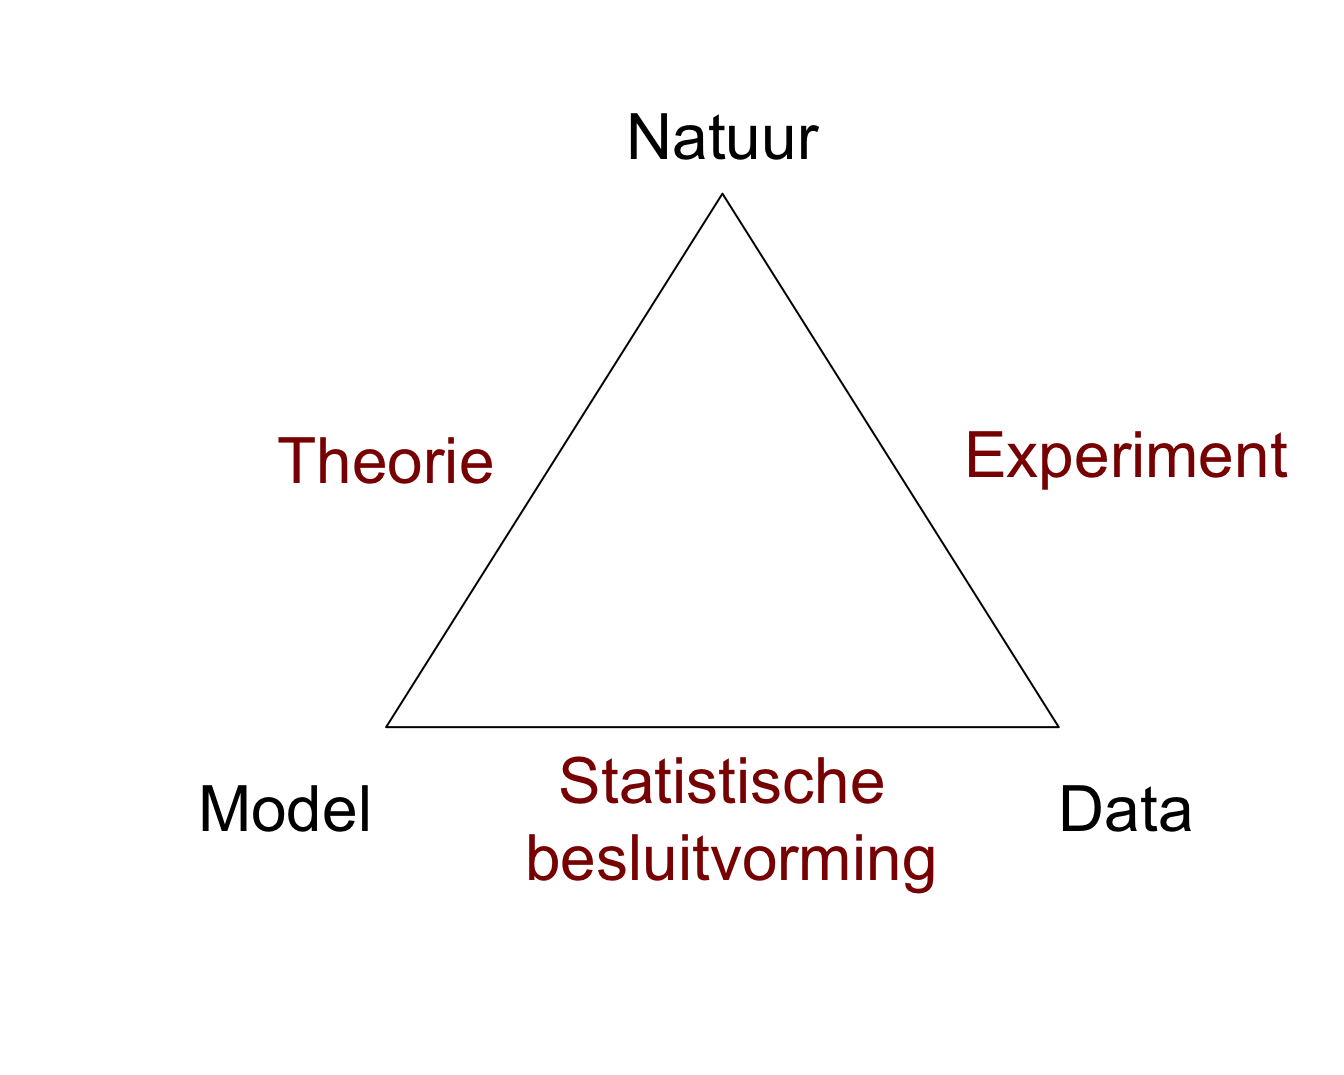
\includegraphics[width=1\linewidth]{Statistiek_2020_2021_files/figure-latex/wetMet-1} 

}

\caption{De Wetenschappelijke Methode en de rol van Statistiek.}\label{fig:wetMet}
\end{figure}

Een andere belangrijke rol van de Statistiek die verder in deze cursus wordt behandeld, is om de \emph{reproduceerbaarheid} van wetenschappelijk onderzoek te waarborgen, binnen zelf gekozen probabiliteitsgrenzen (onzekerheid / zekerheid).

\hypertarget{boutade-met-statistiek-kan-je-alles-bewijzen}{%
\section{Boutade: met statistiek kan je alles bewijzen}\label{boutade-met-statistiek-kan-je-alles-bewijzen}}

In de introductie tonen we aan dat je met statistiek niets kan bewijzen. Statistiek is een hulpmiddel om te leren uit data en om op een reproduceerbare manier conclusies te trekken uit empirisch onderzoek.
Het is eerder zo dat men met foute toepassing van de statistiek alles probeert te bewijzen!

\hypertarget{opzet-van-de-cursus}{%
\section{Opzet van de cursus}\label{opzet-van-de-cursus}}

We leven in een tijd van big data en het is cruciaal om informatie uit cijfers te kunnen extraheren. Statistiek is nu net de wetenschap om te leren uit empirische gegevens.

Statistische geletterdheid is dus een noodzaak om de resultaten uit deze analyses in wetenschappelijke tijdschriften of in de media kritisch te kunnen interpreteren.

Hierbij is het belangrijk om inzicht te verwerven in statistische data analyse enerzijds en om anderzijds deze analyse te interpreteren. We moeten de analyse m.a.w. kunnen koppelen aan de context van het onderzoek: de onderzoeksvraag, de proefopzet en de eigenschappen van de data.
Daarom gaan we alle statistische methodes in de cursus aanbrengen aan de hand van case studies.
We gaan hierbij steeds stilstaan bij

\begin{enumerate}
\def\labelenumi{\arabic{enumi}.}
\item
  de proefopzet en context van de studie (experimenteel ontwerp),
\item
  eigenschappen van de ruwe data (data exploratie), en
\item
  hoe we de resultaten uit de steekproef kunnen veralgemenen naar de populatie toe (statistische besluitvorming).
\item
  Om statistische geletterdheid te verwerven is het ook cruciaal om zelf eenvoudige statistische analyses uit te kunnen voeren zodat je data leert analyseren en te interpreteren. We zullen dus ook in elke case study stilstaan bij hoe we de data analyse uit moeten voeren in statistische software.
\end{enumerate}

In de cursus maken we hiervoor gebruik van
het statistische software pakket R. De cursus en de case studies werden volledig in rmarkdown aangemaakt, dit zijn geavanceerde scripts die toelaten om

\begin{itemize}
\tightlist
\item
  tekst
\item
  formules
\item
  code en
\item
  R output en plots
\end{itemize}

op een efficiënte manier te combineren. Het rmarkdown script kan dan worden gecompileerd naar een webpagina of een pdf document. Op deze manier kan je een data analyse op een volledig reproduceerbare manier documenteren. De scripts van de cursus vormen een goede inspiratiebron om zelf met rmarkdown aan de slag te gaan.

De cursus wordt volledig in online leerpaden verzorgt op het platform Dodona.
Daarbij gaan we hand-on leren statistische programmeren in 2 modules:

\begin{enumerate}
\def\labelenumi{\arabic{enumi}.}
\item
  Module: Introduction to R, waarbij jullie interactief kennis maken met het statistische software pakket en programmeer taal R. Week 1 - Week 3.
\item
  Module: Data exploration and visualisation waarbij jullie de basis principes zullen leren van het maken van goede grafieken die je inzicht zullen geven in de data die wordt gegenereerd in het experiment. Week 4 - 5.
\item
  Module: Statistiek, het hart van deze cursus, waarin jullie inzicht zullen verwerven in de drie belangrijke takken van de statistiek. Week 1-12.

  \begin{itemize}
  \tightlist
  \item
    proefopzet ook wel experimental design genoemd,
  \item
    data exploratie
  \item
    statistische besluitvorming ook wel inferentie genoemd.
  \end{itemize}
\end{enumerate}

Hierbij staat steeds een echte dataset centraal zodat jullie de vertaalslag leren maken van de onderzoeksvraag naar statistisch modellen toe om dan na de data analyse de resultaten opnieuw te interpreteren in termen van de onderzoeksvraag.

We zullen ook telkens alle code delen die nodig is om alle data analyses en visualisaties uit te voeren die worden weergegeven in deze cursus.

In deze inleiding introduceren we drie case studies die het belang van statistiek illustreren.

\begin{enumerate}
\def\labelenumi{\arabic{enumi}.}
\item
  Case study I: Het oksel microbiome. In deze case study doorlopen we alle belangrijke stappen van een experimentele study.
\item
  Case study II: Verschil in lichaamslengte tussen vrouwen en mannen. In deze studie zal je inzicht verwerven in hoe observaties, resultaten en conclusies van een studie onderhevig zijn aan variabiliteit.
\item
  Case study III: Salk vaccin studie voor polio. Deze studie illustreert het belang van een goede controle en introduceert het concept van confounding.
\end{enumerate}

Tijdens de eerste lezing van dit hoofdstuk is het nog niet belangrijk om te focussen op de code. Probeer vooral inzicht te verwerven in het theoretisch raamwerk dat wordt geïntroduceerd. Na week 4 kan het nuttig zijn om de case studies nog eens door te nemen met het oog op hoe je de analyses concreet uit kan voeren.

\hypertarget{case-study-oksel-microbiome}{%
\section{Case study: oksel microbiome}\label{case-study-oksel-microbiome}}

\url{https://www.vrt.be/vrtnws/nl/2018/10/22/gezocht-mensen-met-penetrante-lijfgeur-om-probiotische-deodor/}

Zweten en vooral een zweetgeur is vervelend.
Het zweten op zich is niet de oorzaak van de geur.
Het zijn de microorganismen onder de oksel die het zweet metaboliseren die de geur veroorzaken.
De samenstelling van de gemeenschap van microorganismen onder de oksel is dus bepalend voor het hebben van een zweetgeur.
Deze gemeenschap wordt ook het oksel microbiome genoemd.

Corynebacterium is een bacterië die zweet metaboliseert en hierbij verzadigde vetzuren aanmaakt met een penetrante geur.
Gelukkig zijn er Staphylococcus bacteriën die het zweet ook metaboliseren maar die hierbij geen hinderlijke verzadigde vetzuren produceren.

Het CMet Lab aan de Universiteit Gent doet onderzoek naar microbiële gemeenschappen en stelde een therapie voor om mensen van dit probleem af te helpen.
Die bestaat uit een antibiotica behandeling van de oksel om microbiome af te doden,
gevolgd door een transplantatie van het microbiome van een persoon zonder zweetgeur.

Alvorens dat de therapie breed kan worden ingezet, dient eerst te worden aangetoond in een experiment dat ze werkt.

\hypertarget{experimenteel-design-proefopzet}{%
\subsection{Experimenteel design (proefopzet)}\label{experimenteel-design-proefopzet}}

Een eerste tak van de statistiek focust op experimenteel design.
Idealiter zouden we de therapie evalueren door het uit te testen op de volledige populatie van personen met een zweetgeur.
Dat is echter niet haalbaar omdat het

\begin{enumerate}
\def\labelenumi{\arabic{enumi}.}
\tightlist
\item
  ethisch niet verantwoord is: we weten niet of therapie werkt
\item
  financieel en logistiek onmogelijk is om iedereen te bemonsteren, en omdat
\item
  de populatie waarover we uitspraken wensen te doen bestaat nog niet volledig: ze omvat ook toekomstige personen met een zweetgeur.
\end{enumerate}

Daarom zullen we een steekproef nemen.
Hierbij zullen we een aantal personen uit de populatie selecteren waarop we het experiment uit zullen voeren.

Cruciaal is hierbij dat de steekproef representatief is voor de populatie zodat we de resultaten van het experiment zullen kunnen veralgemenen naar de populatie. We zullen de mensen daarom volledig at random trekken uit de populatie zodat elk subject een zelfde kans heeft om in het experiment te worden opgenomen: randomisatie.
Merk ook op dat het daarom heel belangrijk om de populatie goed te omschrijven voor de start van het experiment: scope van de studie.

In deze studie worden twintig personen met een zweetgeur volledig at random geselecteerd uit de populatie.
We zouden nu elk subject kunnen behandelen.
Maar, dan zijn we niet zeker dat een verschil in het microbiome te wijten is aan de behandeling.

We hebben dus een goeie controle nodig.
We zouden de controle personen niet kunnen behandelen, maar dan kan een verschil in microbiome mogelijks ook te wijten zijn aan de antibiotica behandeling i.p.v. aan de transplantatie.
De onderzoekers opteerden daarom 10 personen een placebo behandeling geven, enkel antibiotica behandeling en 10 personen te behandelen met antibiotica en de transplantatie.

De proefpersonen worden volledig at random toegewezen aan de behandelingsgroep zodat beide groepen vergelijkbaar zijn.

Vervolgens moet er stil worden gestaan bij hoe het microbiome zal worden gemeten?

In de studie maakte men gebruik van een DGGE meting.
Microorganismen hebben een heel variabel stukje ribosomaal RNA, het 16s ribosomaal RNA dat uniek is voor de soort.
Het 16S rRNA van de verschillende microorganismen in het staal wordt dan geamplificeerd en gescheiden op een DGGE gel.
Waarbij een bandenpatroon ontstaat volgens de lengte van het 16s rRNA.

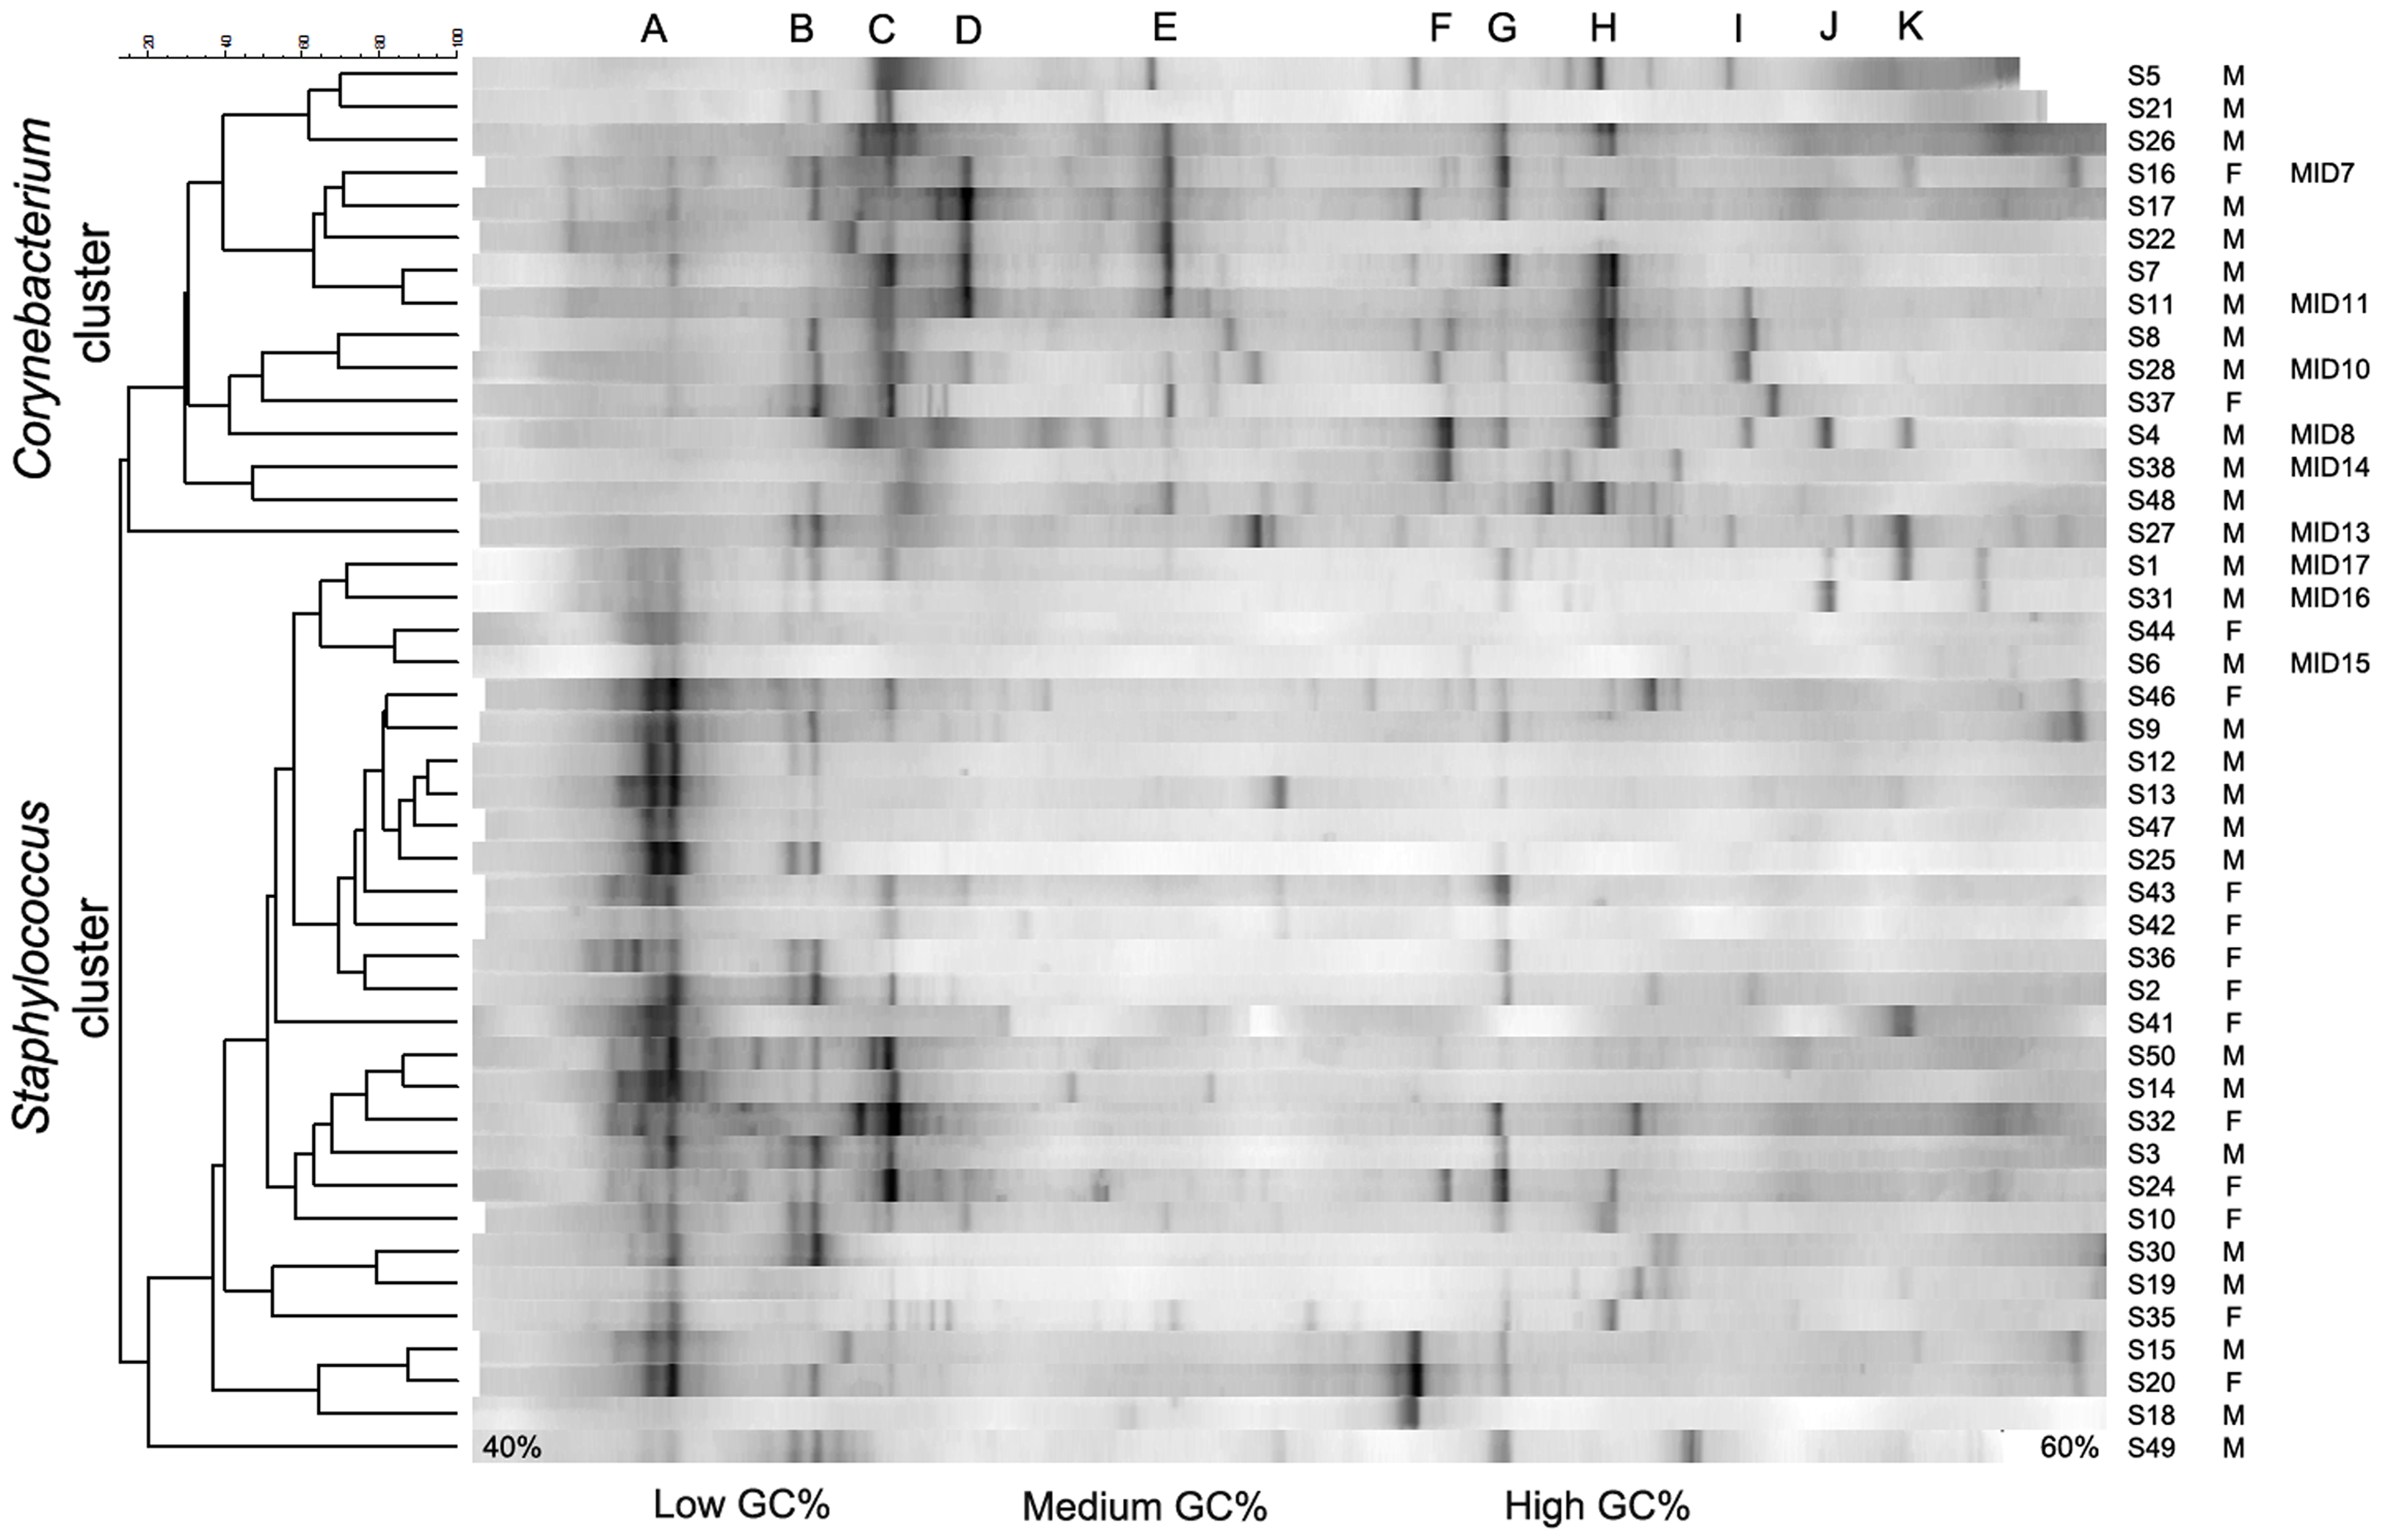
\includegraphics[width=0.7\textwidth,height=\textheight]{../figures/dgge.png}
Foto van een DGGE gel van het oksel microbiome (bron: \url{https://doi.org/10.1371/journal.pone.0070538})

Elke band in de DGGE correspondeert met een bacterie.
Hoe helderder de band hoe meer van de bacterie in het microbiome voorkomt.
Band A staat voor Staphylococcus.
De ratio van de intensiteit van de band en de totale intensiteit in het bandenpatroon kan worden gebruik als een proxy voor de relatieve abundantie.

\emph{Essentiële stap: Vertaal onderzoeksvraag nu naar iets wat we kunnen quantificeren!}

We kunnen dit doen door middel van het gemiddeld verschil in relatieve abundantie in Staphylococcus tussen de transplantatie en placebo groep.

Het experiment kan nu worden uitgevoerd.

\hypertarget{data-exploratie-en-beschrijvende-statistiek}{%
\subsection{Data exploratie en beschrijvende statistiek}\label{data-exploratie-en-beschrijvende-statistiek}}

Data exploratie is heel belangrijk om inzicht te krijgen in de data en is een essentiële eerste stap om te leren uit data.
Het wordt vaak ondergewaardeerd of over het hoofd gezien.

Data in deze cursus wordt verwerkt via het statistisch software pakket R.
Vooraleer we met de data exploratie van start kunnen gaan moeten we de data eerst importeren in R.

We geven duidelijk aan welke delen van de tekst over het Code gaan en welke over de interpretatie. Probeer initiëel te focussen op de interpretatie. Het Code zal je immers gedurende de eerste weken oppikken. Daarom hebben we ook gekozen om aparte clips te maken m.b.t interpretatie en Code. Zodat de manier hoe je de data analyse dient uit te voeren het begrip initiëel niet in de weg staan.

\hypertarget{importeer-de-data}{%
\subsubsection{Importeer de data}\label{importeer-de-data}}

\emph{Code} Tijdens de data exploratie gaan we voor de data manipulaties veelal gebruik maken van functies uit het \texttt{tidyverse} package.
Dat kan worden geladen door het commando
\texttt{library(tidyverse)}.

Via het commando \texttt{read\_lines} kunnen we enkele regels van een data bestand inlezen om de structuur van het data bestand te weten te komen.

\begin{Shaded}
\begin{Highlighting}[]
\KeywordTok{library}\NormalTok{(tidyverse)}
\KeywordTok{read\_lines}\NormalTok{(}\StringTok{"https://raw.githubusercontent.com/statOmics/sbc20/master/data/armpit.csv"}\NormalTok{)}
\end{Highlighting}
\end{Shaded}

\begin{verbatim}
##  [1] "trt,rel"                       "placebo,54.99207606973059"    
##  [3] "placebo,31.84466019417476"     "placebo,41.09947643979057"    
##  [5] "placebo,59.52063914780293"     "placebo,63.573407202216075"   
##  [7] "placebo,41.48648648648649"     "placebo,30.44041450777202"    
##  [9] "placebo,42.95676429567643"     "placebo,41.7391304347826"     
## [11] "placebo,33.896515311510036"    "transplant,57.218124341412015"
## [13] "transplant,72.50900360144058"  "transplant,61.89258312020461" 
## [15] "transplant,56.690140845070424" "transplant,76"                
## [17] "transplant,71.7357910906298"   "transplant,57.757296466973884"
## [19] "transplant,65.1219512195122"   "transplant,67.53424657534246" 
## [21] "transplant,77.55359394703657"
\end{verbatim}

We observeren de volgende structuur:

\begin{itemize}
\tightlist
\item
  Gegevens in het bestand zijn door comma's gescheiden.
\item
  Elke rij bevat de gegevens voor 1 proefpersoon
\item
  Verschillende variabelen worden gemeten per persoon en zijn van elkaar gescheiden door een comma. Het bestand is in csv formaat: ``comma separated values''.
\item
  We kunnen bestanden met dit formaat inlezen R via het commando \texttt{read\_csv}.
\item
  We slaan de data op in R in het object met naam ap. Hiervoor gebruiken we de \texttt{\textless{}-} operator.
\item
  We geven de data tabel terug door het object aan te roepen door zijn naam te typen.
\end{itemize}

\begin{Shaded}
\begin{Highlighting}[]
\NormalTok{ap \textless{}{-}}\StringTok{ }\KeywordTok{read\_csv}\NormalTok{(}\StringTok{"https://raw.githubusercontent.com/statOmics/sbc20/master/data/armpit.csv"}\NormalTok{)}
\NormalTok{ap}
\end{Highlighting}
\end{Shaded}

\begin{verbatim}
## # A tibble: 20 x 2
##    trt          rel
##    <chr>      <dbl>
##  1 placebo     55.0
##  2 placebo     31.8
##  3 placebo     41.1
##  4 placebo     59.5
##  5 placebo     63.6
##  6 placebo     41.5
##  7 placebo     30.4
##  8 placebo     43.0
##  9 placebo     41.7
## 10 placebo     33.9
## 11 transplant  57.2
## 12 transplant  72.5
## 13 transplant  61.9
## 14 transplant  56.7
## 15 transplant  76  
## 16 transplant  71.7
## 17 transplant  57.8
## 18 transplant  65.1
## 19 transplant  67.5
## 20 transplant  77.6
\end{verbatim}

Als we data matrix observeren zien we de volgende structuur:
proefpersonen in de rijen waarvoor we twee karateristieken (variabelen) hebben bijgehouden per subject:
behandeling (trt) en relatieve abundantie (rel).
Deze data structuur wordt \texttt{tidy\ data} genoemd.

Weinig mensen kunnen a.d.h.v. het bekijken van de data matrix structuur of patronen zien in de data. Daarom zullen we de data moeten verwerken en visualiseren.

\hypertarget{beschrijvende-statistiek}{%
\subsubsection{Beschrijvende statistiek}\label{beschrijvende-statistiek}}

In artikels en de media worden resultaten uit een steekproef vaak gerapporteerd a.d.h.v. gemiddelde en de standaardafwijking.

\emph{Code}

\begin{itemize}
\tightlist
\item
  We vatten de data eerst samen. We berekenen het gemiddelde en de standaard deviatie (een maat voor de spreiding, zie volgende hoofdstukken).
  We slaan het resultaat hiervan op in het object apRelSum via \texttt{apRelSum\ \textless{}-}.
\end{itemize}

\begin{enumerate}
\def\labelenumi{\arabic{enumi}.}
\item
  We pipen (via \texttt{\%\textgreater{}\%}) het \texttt{ap} dataframe naar de \texttt{group\_by} functie om de data te groeperen per treatment trt: \texttt{group\_by(trt)}.
\item
  We pipen het resultaat naar de \texttt{summarize\_at} function om de ``rel'' variable samen te vatten en berekenen hierbij het gemiddelde en standaardafwijking. Omdat we de data eerst hebben gegroepeerd zullen we het gemiddelde en de standaard deviatie berekenen per groep.
\end{enumerate}

\begin{Shaded}
\begin{Highlighting}[]
\NormalTok{apRelSum \textless{}{-}}\StringTok{ }\NormalTok{ap }\OperatorTok{\%\textgreater{}\%}\StringTok{ }\KeywordTok{group\_by}\NormalTok{(trt) }\OperatorTok{\%\textgreater{}\%}\StringTok{ }\KeywordTok{summarize\_at}\NormalTok{(}\StringTok{"rel"}\NormalTok{, }
    \KeywordTok{list}\NormalTok{(}\DataTypeTok{mean =}\NormalTok{ mean, }\DataTypeTok{sd =}\NormalTok{ sd))}
\end{Highlighting}
\end{Shaded}

We tonen vervolgens het resultaat door het object apRelSum aan te roepen

\begin{Shaded}
\begin{Highlighting}[]
\NormalTok{apRelSum}
\end{Highlighting}
\end{Shaded}

\begin{verbatim}
## # A tibble: 2 x 3
##   trt         mean    sd
##   <chr>      <dbl> <dbl>
## 1 placebo     44.2 11.5 
## 2 transplant  66.4  7.88
\end{verbatim}

We kunnen ook een tabel in de webpagina of het pdf bestand integreren via het commando kable van het knitr pakket:

\begin{Shaded}
\begin{Highlighting}[]
\NormalTok{knitr}\OperatorTok{::}\KeywordTok{kable}\NormalTok{(apRelSum, }\StringTok{"html"}\NormalTok{)}
\end{Highlighting}
\end{Shaded}

trt

mean

sd

placebo

44.15496

11.543251

transplant

66.40127

7.880175

\emph{Interpretatie}

Het effect van de behandeling in de steekproef kan worden gekwantificeerd door de gemiddelde relatieve abundantie te vergelijken in elke steekproef. We observeren dat de gemiddelde relatieve abundantie in de steekproef gemiddeld 22.2\% hoger is in de transplantatie dan in de placebo groep.

We quantificeren ook de variabiliteit of de spreiding van de gegevens rond het gemiddelde aan de hand van de standaardafwijking.

Het gemiddelde en de standaardafwijking wordt ook vaak grafisch weergegeven in een barplot.

\emph{Code}
We maken in deze cursus gebruik van het pakket \texttt{ggplot2} om grafieken te maken.\\
Met de ggplot2 bibliotheek kunnen we gemakkelijk grafieken opbouwen in lagen (layers).
Hierdoor leest de code veel makkelijker.
In uitgebreide introductie tot ggplot vinden je in de Dodona module \href{https://dodona.ugent.be/nl/courses/345/}{R data exploration and visualisation}.

Bar plots worden heel veel gebruikt in artikels om resultaten weer te geven.

\begin{enumerate}
\def\labelenumi{\arabic{enumi}.}
\item
  We pipen de samengevatte data naar de functie \texttt{ggplot}. Dat is de basis van elke ggplot. We selecteren de variabele met de behandeling trt als x variabele en de variabele met naam mean als y-variabele voor de plot.
  We doen dit steeds via de aestetics \texttt{aes} functie. \texttt{aes(x=trt,y=mean)}
\item
  We maken een barplot door een laag toe te voegen via de \texttt{geom\_bar} function. De statistiek is \texttt{stat="identity"} omdat de hoogte van de bar gelijk is aan de waarde voor y (hier het gemiddelde voor de relatieve abundantie).
\item
  We voegen foutenvlaggen toe om de onzekerheid op het gemiddelde weer te geven. We doen dit via de \texttt{geom\_errorbar} functie en specifiëren het minimum en maximum van de error bar. Het \texttt{width} argument wordt gebruikt om de breedte van de error bar smaller te maken dat deze van de bar.
\end{enumerate}

\begin{Shaded}
\begin{Highlighting}[]
\NormalTok{apRelSum }\OperatorTok{\%\textgreater{}\%}\StringTok{ }\KeywordTok{ggplot}\NormalTok{(}\KeywordTok{aes}\NormalTok{(}\DataTypeTok{x =}\NormalTok{ trt, }\DataTypeTok{y =}\NormalTok{ mean)) }\OperatorTok{+}\StringTok{ }\KeywordTok{geom\_bar}\NormalTok{(}\DataTypeTok{stat =} \StringTok{"identity"}\NormalTok{) }\OperatorTok{+}\StringTok{ }
\StringTok{    }\KeywordTok{geom\_errorbar}\NormalTok{(}\KeywordTok{aes}\NormalTok{(}\DataTypeTok{ymin =}\NormalTok{ mean }\OperatorTok{{-}}\StringTok{ }\NormalTok{sd, }\DataTypeTok{ymax =}\NormalTok{ mean }\OperatorTok{+}\StringTok{ }
\StringTok{        }\NormalTok{sd), }\DataTypeTok{width =} \FloatTok{0.2}\NormalTok{)}
\end{Highlighting}
\end{Shaded}

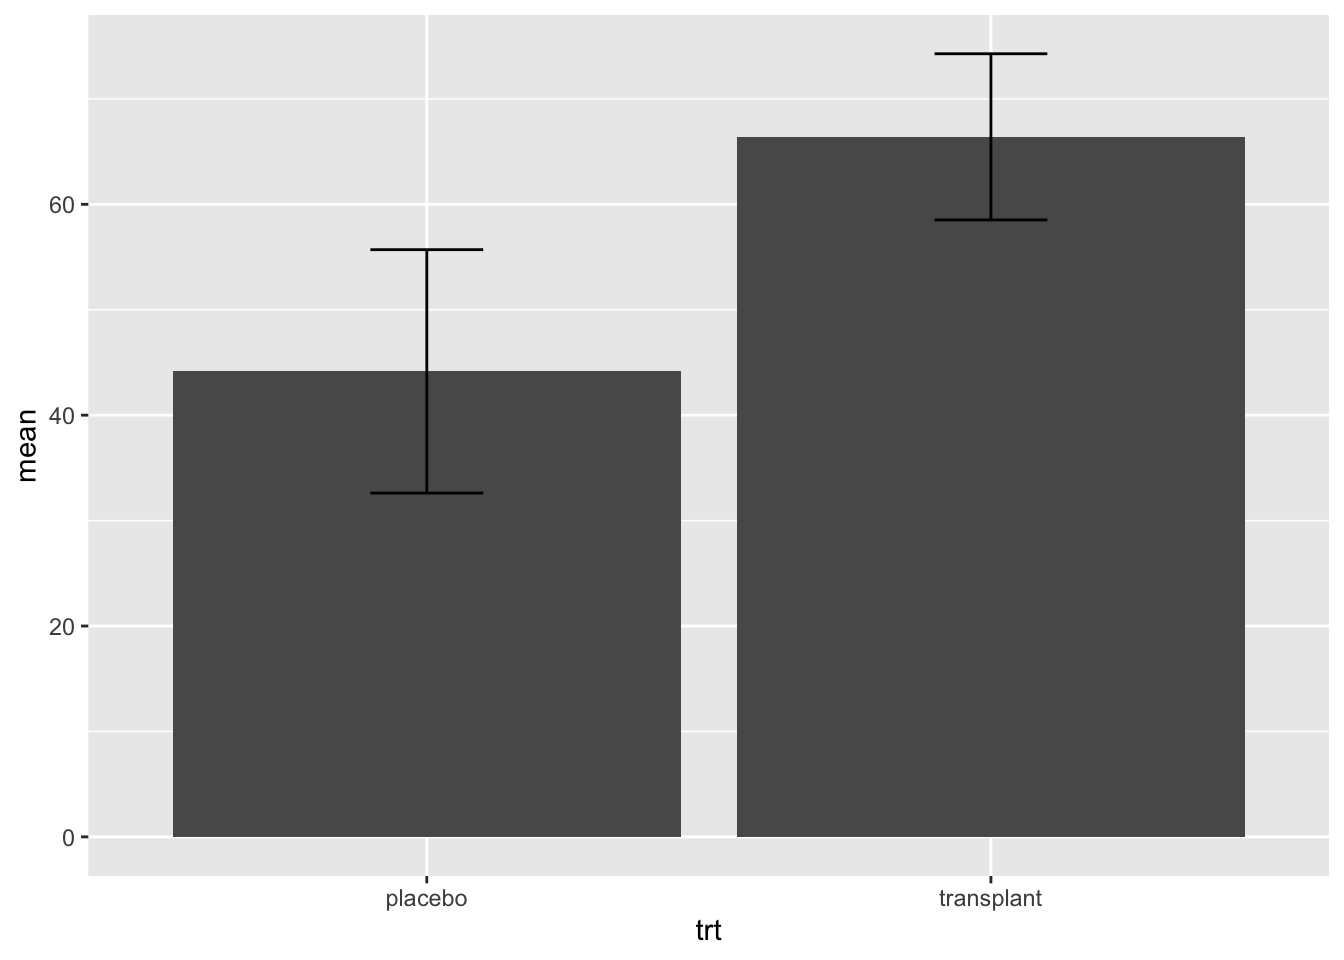
\includegraphics{Statistiek_2020_2021_files/figure-latex/unnamed-chunk-7-1.pdf}

\emph{Interpretatie}

Is deze plot informatief? Nee!

We zien enkel een ``two-number summary'': het gemiddelde en de standaarddeviatie. We weten niet of deze wel een goeie samenvattende maat zijn voor de data. Bovendien wordt heel wat ruimte in de plot benut die niet informatief is: er zijn bijvoorbeeld geen observaties met relatieve abundanties van 0\%.

Om de data van verschillende groepen makkelijk te kunnen vergelijken in een grafiek die meer informatief is dan de bar plot ontwikkelde Tukey de boxplot. Dit is een ``five-number summary'' het bereik van de data (minimum en maximum) samen met het 25, 50 (mediaan), and 75 percentiel. Deze percentielen zijn de waarden waarvoor respectievelijk 25\%, 50\% en 75\% van de data in de steekproef kleiner zijn. Tukey raadde aan om het bereik van de data te berekenen zonder rekening te houden met outliers (extreme observaties). De outliers worden afzonderlijk als data punten toegevoegd aan de plot. In het hoofdstuk 4: Data Exploratie leggen we uit wat outliers precies zijn.

\emph{Code}
We maken nu een boxplot voor de ap data

\begin{enumerate}
\def\labelenumi{\arabic{enumi}.}
\tightlist
\item
  We pipen het \texttt{ap} data object naar \texttt{ggplot}
\item
  We selecteren de data voor de plot via \texttt{ggplot(aes(x=trt,y=rel))}
\item
  We voegen een laag toe voor de boxplot dmv de functie \texttt{geom\_boxplot()}
\end{enumerate}

\begin{Shaded}
\begin{Highlighting}[]
\NormalTok{ap }\OperatorTok{\%\textgreater{}\%}\StringTok{ }\KeywordTok{ggplot}\NormalTok{(}\KeywordTok{aes}\NormalTok{(}\DataTypeTok{x =}\NormalTok{ trt, }\DataTypeTok{y =}\NormalTok{ rel)) }\OperatorTok{+}\StringTok{ }\KeywordTok{geom\_boxplot}\NormalTok{()}
\end{Highlighting}
\end{Shaded}

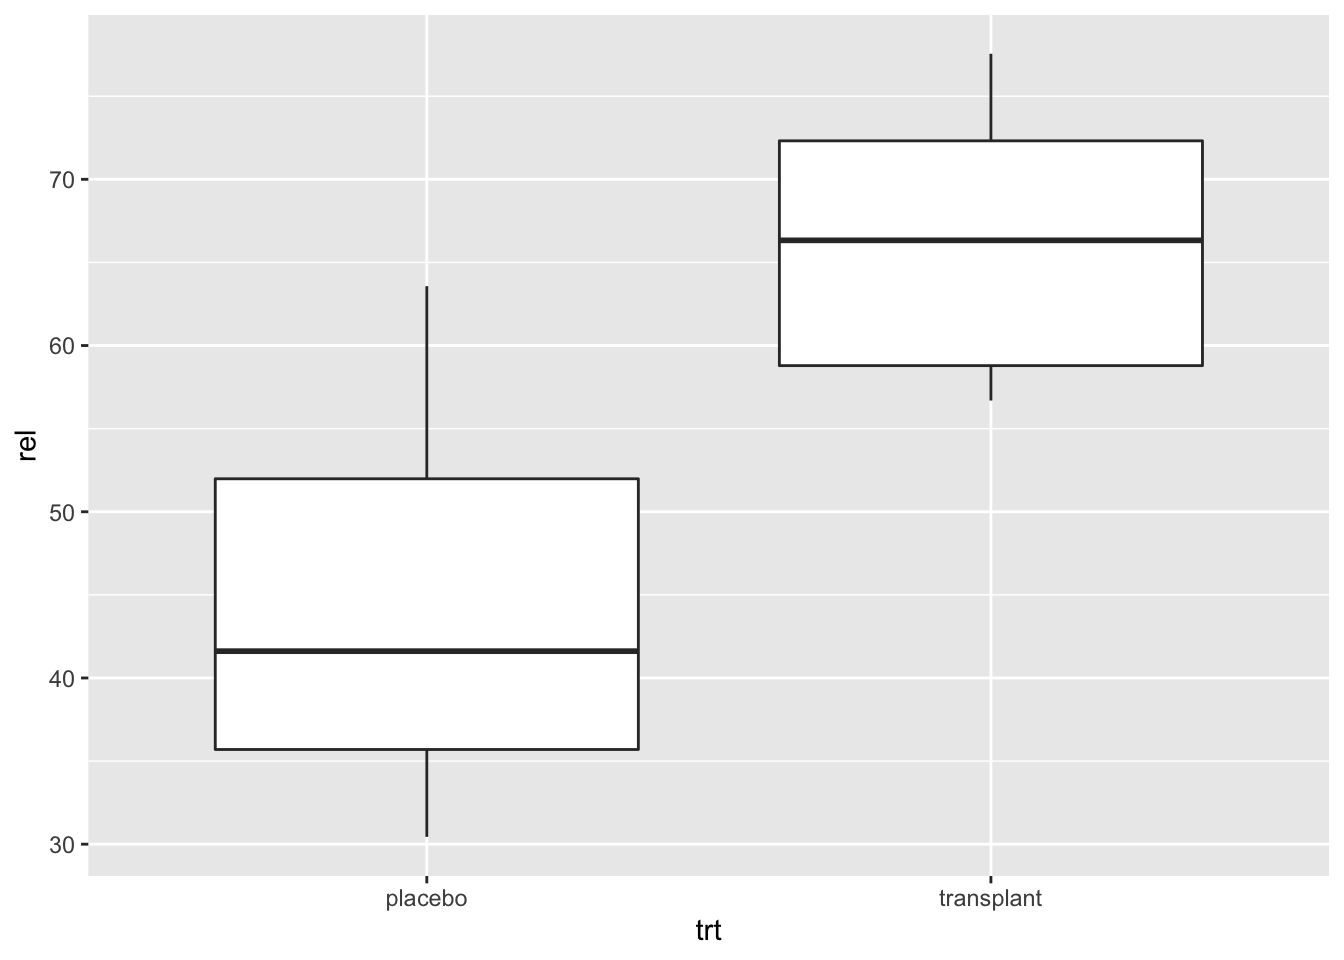
\includegraphics{Statistiek_2020_2021_files/figure-latex/unnamed-chunk-8-1.pdf}

\emph{Interpretatie}: De boxplot geeft ons al veel meer informatie dan de barplot. Het bereik van de data wordt weergegeven door de wiskers (eindpunten van de verticale lijnen in het midden van de boxplot). De box in de boxplot geeft het 25\%, 50\% en 75\% percentiel weer. (Merk op dat er geen outliers zijn. Er worden geen individuele punten weergegeven in de plot)

We observeren dat boxplot voor de transplantie groep hoger ligt dan voor de placebo groep. Wat aangeeft dat de relatieve abundanties van Staphylococcus vaak hoger liggen voor personen in de steekproef die zijn toegewezen aan de transplantatie groep dan voor personen die zijn toegewezen aan placebo groep. Dit is een indicatie dat de behandeling werkt.

Verder weten we dat er maar 10 observaties zijn in elke groep. Dat laat toe om de ruwe gegevens aan de plot toe te voegen zonder dat de plot te druk wordt.

\emph{Code}

\begin{itemize}
\tightlist
\item
  Merk op dat we het argument \texttt{outlier.shape} op NA (not available) zetten \texttt{outlier.shape=NA} in the \texttt{geom\_boxplot} functie. Dat doen we standaard als we de ruwe data toevoegen aan de boxplots: anders zullen outliers immers twee keer worden weergegeven (eerst via de boxplot laag en daarna door de laag met alle ruwe data toevoegen aan de plot).
\item
  We geven de ruwe data weer via de \texttt{geom\_point(position="jitter")} functie. We gebruiken hierbij het argument position=`jitter' zodat we wat random ruis toevoegen aan de x-cordinaat zodat de gegevens elkaar niet overlappen.
\end{itemize}

\begin{Shaded}
\begin{Highlighting}[]
\NormalTok{ap }\OperatorTok{\%\textgreater{}\%}\StringTok{ }\KeywordTok{ggplot}\NormalTok{(}\KeywordTok{aes}\NormalTok{(}\DataTypeTok{x =}\NormalTok{ trt, }\DataTypeTok{y =}\NormalTok{ rel)) }\OperatorTok{+}\StringTok{ }\KeywordTok{geom\_boxplot}\NormalTok{(}\DataTypeTok{outlier.shape =} \OtherTok{NA}\NormalTok{) }\OperatorTok{+}\StringTok{ }
\StringTok{    }\KeywordTok{geom\_point}\NormalTok{(}\DataTypeTok{position =} \StringTok{"jitter"}\NormalTok{)}
\end{Highlighting}
\end{Shaded}

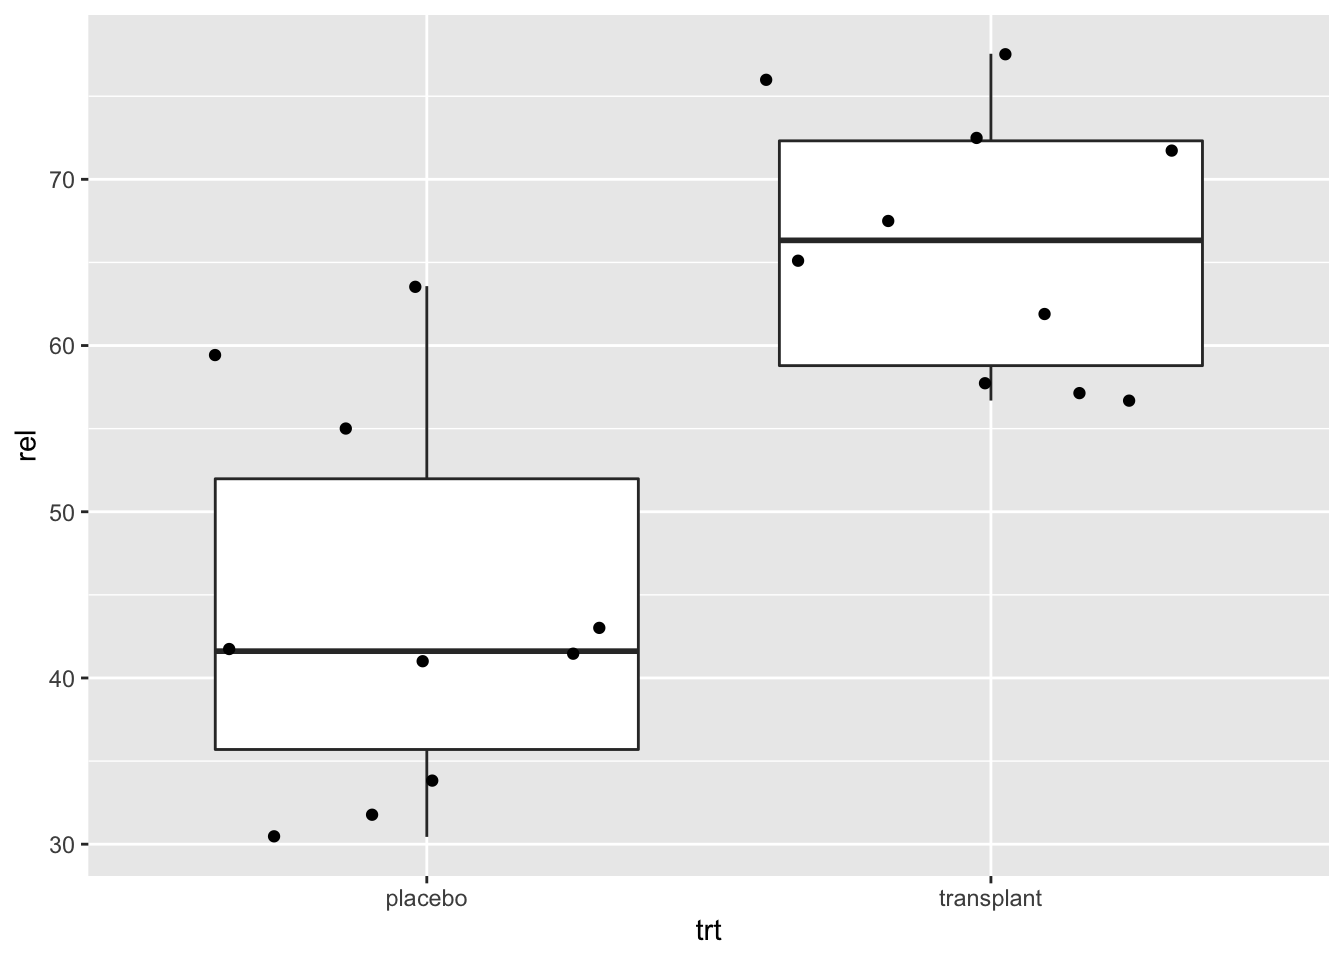
\includegraphics{Statistiek_2020_2021_files/figure-latex/unnamed-chunk-9-1.pdf}

Dit is een informatieve plot!
Het toont de data zo ruw mogelijk weer. De plot is toch nog goed leesbaar en toont duidelijk aan dat de relatieve abundanties bij bijna alle proefpersonen in de transplantatie groep hoger is dan deze voor de placebo groep.

\hypertarget{statistische-besluitvorming}{%
\subsection{Statistische Besluitvorming}\label{statistische-besluitvorming}}

We zagen duidelijk een effect van de transplantatie op de relatieve abundantie van Staphylococcus.
We vragen ons nu af of het effect groot genoeg om te kunnen concluderen dat de behandeling werkt?

Hoe kunnen we met andere woorden de conclusies uit de steekproef veralgemenen naar de populatie toe? \emph{inductie}.
Op basis van de steekproef kunnen we het effect, gemiddeld verschil in relatieve abundantie tussen beide behandelingsgroepen, schatten in de populatie.
De prijs die we hiervoor betalen is onzekerheid!
Omdat we niet alle personen in de populatie hebben kunnen testen zullen we echter nooit absoluut zeker kunnen zijn over onze conclusies.

Om de conclusies uit de steekproef te veralgemenen naar de populatie maken we gebruik van een derde tak van de statistiek:
Statistische besluitvorming.

\begin{itemize}
\item
  Met data kunnen we niet bewijzen dat een behandeling werkt.
\item
  Falsificatie principe van Popper: Data kunnen enkel een hypothese of een theorie ontkrachten.
\item
  Met statistiek kunnen we dus niet aantonen dat de behandeling werkt.
\item
  Statistiek zal ons wel toelaten om het omgekeerde te falsifiëren: als we veronderstellen dat er geen effect van de behandeling, spreekt de data in de steekproef dit tegen?
\end{itemize}

Met statistiek kunnen we berekenen hoe waarschijnlijk het is om in een random steekproef (nieuw experiment) een verschil in gemiddelde relatieve abundantie te zien tussen transplantatie (\(\bar X_\text{transplant}\)) en placebo groep (\(\bar X_\text{placebo}\)) dat minstens 22.2\% bedraagt als de behandeling geen effect zou hebben.

\[p=P( \vert \bar X_\text{transplant}-\bar X_\text{placebo}\vert \vert \geq 22.2\% \vert \text{geen effect van de behandeling})\]

\begin{itemize}
\item
  Die kans wordt een p-waarde genoemd.
\item
  Als p heel klein is, dan is het heel onwaarschijnlijk om een dergelijk effect door toeval te observeren in een steekproef als er in werkelijkheid geen effect is van de behandeling.
\end{itemize}

Om de kans p te berekenen is het nodig om de data te modelleren met een statistisch model. Hiervoor zullen we bepaalde aannames moeten doen. In hoofdstuk 5 zien we dat we dit kunnen doen d.m.v. de \texttt{t.test} functie.

\begin{Shaded}
\begin{Highlighting}[]
\KeywordTok{t.test}\NormalTok{(rel }\OperatorTok{\textasciitilde{}}\StringTok{ }\NormalTok{trt, }\DataTypeTok{data =}\NormalTok{ ap)}
\end{Highlighting}
\end{Shaded}

\begin{verbatim}
## 
##  Welch Two Sample t-test
## 
## data:  rel by trt
## t = -5.0334, df = 15.892, p-value = 0.0001249
## alternative hypothesis: true difference in means is not equal to 0
## 95 percent confidence interval:
##  -31.62100 -12.87163
## sample estimates:
##    mean in group placebo mean in group transplant 
##                 44.15496                 66.40127
\end{verbatim}

Als er in werkelijkheid geen effect is van de behandeling en als de model aannames correct zijn dan verwachten we in minder dan 2 op 10000 random steekproeven een verschil van minstens 22.2\% in de relatieve abundantie tussen beide behandelingsgroepen.
Deze kans is heel klein. Het is dus heel onwaarschijnlijk om dergelijk verschil in relatieve abundantie te observeren in een random steekproef als er geen effect van de behandeling zou zijn.

We kunnen daarom de hypothese dat er geen effect is van de behandeling verwerpen en concluderen:

Er is een statistisch significant verschil in gemiddelde relatieve abundantie van Staphylococcus in het okselmicrobiome van personen met een zweetgeur die worden behandeld met de transplantie en personen die behandeld worden met de placebo behandeling.
Gemiddeld is de relatieve abundantie van Staphylococcus in het microbiome van personen met een zweetgeur is 22.2\% hoger na microbiome transplantie dan na de placebo behandeling.

\hypertarget{mogelijke-fouten}{%
\subsubsection{Mogelijke fouten}\label{mogelijke-fouten}}

Merk op dat een experiment onderhevig is aan random variabiliteit. Als we het experiment opnieuw uit zouden voeren zullen we andere proefpersonen in de steekproef opnemen. Bijgevolg zullen we ook andere relatieve abundanties meten.

\begin{itemize}
\item
  Daardoor zijn ook onze conclusies onderhevig aan random variabiliteit.
\item
  Zelfs al zou er in werkelijkheid geen effect zijn van de behandeling dan kunnen we in een random steekproef met 10 mensen in de placebo en 10 mensen in de behandelingsgroep toch ook een verschil in relatieve abundantie observeren die minsten 22.2\% is. Dat kunnen we in 1 op de 10000 experimenten verwachten.
\end{itemize}

In dergelijke steekproef zal men ten onrechte besluiten dat er bewijs is dat de transplantie behandeling werkt.

\begin{itemize}
\item
  Intuïtief voelen we aan dat we dus niet met absolute zekerheid uitspraken kunnen doen over populatiekarakteristieken op basis van een eindige steekproef.
\item
  Typisch zullen we de p-waarde vergelijken met 5\% vooraleer we beslissen dat een behandeling werkt. We zullen de kans op het maken van foute conclusies dus controleren op 5\%.
\end{itemize}

In de volgende case studie zullen we bestuderen hoe de metingen, de resultaten en de conclusies kunnen variëren van steekproef tot steekproef.

\hypertarget{case-study-ii-verschil-in-lengte-tussen-vrouwen-en-mannen}{%
\section{Case Study II: Verschil in lengte tussen vrouwen en mannen}\label{case-study-ii-verschil-in-lengte-tussen-vrouwen-en-mannen}}

Om resultaten van een steekproef te kunnen veralgemenen naar de populatie toe trekken we subjecten at random uit de populatie.

Randomisatie is sterk gerelateerd met het concept van de populatie en scope van de studie.
De scope van de studie moet goed worden omschreven voor de start van het experiment. Het is immers de populatie naar waar we de resultaten uit de steekproef kunnen veralgemenen.

We nemen daarom een random steekproef uit de populatie:

\begin{itemize}
\item
  alle subjecten van de populatie hebben dus evenveel kans om in de steekproef te worden opgenomen.
\item
  de selectie van een subject is onafhankelijk van andere subjecten in de steekproef.
\end{itemize}

De steekproef is dan representatief voor de populatie, maar is nog steeds random.

Om te begrijpen dat een steekproef random is zouden we hetzelfde experiment veel keer moeten kunnen herhalen (\texttt{repeated\ sampling}). Dan zouden we inzicht kunnen krijgen hoe de gegevens veranderen van steekproef tot steekproef.

Om dit te illustreren zullen we gebruik maken van de National Health And Nutrition Examination Study (NHANES) studie. Uit die studie kunnen we herhaaldelijk kleine steekproeven trekken om te begrijpen hoe de gegevens en statistieken veranderen van steekproef tot steekproef. Of om met andere woorden na te gaan wat de variabiliteit is tussen steekproeven.

De National Health And Nutrition Examination Study (NHANES) studie:

\begin{itemize}
\item
  Sinds 1960 worden elk jaar mensen van alle leeftijden geïnterviewd bij hen thuis.
\item
  Er maakt ook een gezondheidsonderzoek deel uit van de study die in een mobiel onderzoekscentrum wordt afgenomen.
\item
  We zullen deze grote studie gebruiken om at random personen te selecteren van de Amerikaanse populatie.
\item
  Dat zal inzicht geven in hoe de gegevens en resultaten van een analyse zullen variëren van steekproef tot steekproef.
\end{itemize}

De data van deze studie is terug te vinden in het R pakket \texttt{NHANES}. Met de functie \texttt{head} kunnen we de eerste 6 rijen van de dataset bekijken.

\begin{Shaded}
\begin{Highlighting}[]
\KeywordTok{library}\NormalTok{(NHANES)}
\KeywordTok{head}\NormalTok{(NHANES)}
\end{Highlighting}
\end{Shaded}

\begin{verbatim}
## # A tibble: 6 x 76
##      ID SurveyYr Gender   Age AgeDecade AgeMonths Race1 Race3 Education
##   <int> <fct>    <fct>  <int> <fct>         <int> <fct> <fct> <fct>    
## 1 51624 2009_10  male      34 " 30-39"        409 White <NA>  High Sch~
## 2 51624 2009_10  male      34 " 30-39"        409 White <NA>  High Sch~
## 3 51624 2009_10  male      34 " 30-39"        409 White <NA>  High Sch~
## 4 51625 2009_10  male       4 " 0-9"           49 Other <NA>  <NA>     
## 5 51630 2009_10  female    49 " 40-49"        596 White <NA>  Some Col~
## 6 51638 2009_10  male       9 " 0-9"          115 White <NA>  <NA>     
## # ... with 67 more variables: MaritalStatus <fct>, HHIncome <fct>,
## #   HHIncomeMid <int>, Poverty <dbl>, HomeRooms <int>, HomeOwn <fct>,
## #   Work <fct>, Weight <dbl>, Length <dbl>, HeadCirc <dbl>, Height <dbl>,
## #   BMI <dbl>, BMICatUnder20yrs <fct>, BMI_WHO <fct>, Pulse <int>,
## #   BPSysAve <int>, BPDiaAve <int>, BPSys1 <int>, BPDia1 <int>, BPSys2 <int>,
## #   BPDia2 <int>, BPSys3 <int>, BPDia3 <int>, Testosterone <dbl>,
## #   DirectChol <dbl>, TotChol <dbl>, UrineVol1 <int>, UrineFlow1 <dbl>,
## #   UrineVol2 <int>, UrineFlow2 <dbl>, Diabetes <fct>, DiabetesAge <int>,
## #   HealthGen <fct>, DaysPhysHlthBad <int>, DaysMentHlthBad <int>,
## #   LittleInterest <fct>, Depressed <fct>, nPregnancies <int>, nBabies <int>,
## #   Age1stBaby <int>, SleepHrsNight <int>, SleepTrouble <fct>,
## #   PhysActive <fct>, PhysActiveDays <int>, TVHrsDay <fct>, CompHrsDay <fct>,
## #   TVHrsDayChild <int>, CompHrsDayChild <int>, Alcohol12PlusYr <fct>,
## #   AlcoholDay <int>, AlcoholYear <int>, SmokeNow <fct>, Smoke100 <fct>,
## #   Smoke100n <fct>, SmokeAge <int>, Marijuana <fct>, AgeFirstMarij <int>,
## #   RegularMarij <fct>, AgeRegMarij <int>, HardDrugs <fct>, SexEver <fct>,
## #   SexAge <int>, SexNumPartnLife <int>, SexNumPartYear <int>, SameSex <fct>,
## #   SexOrientation <fct>, PregnantNow <fct>
\end{verbatim}

We focussen in dit voorbeeld op het verschil in lengte tussen volwassen vrouwen en mannen in de Amerikaanse populatie.

Onderzoeksvraag: hoe verschilt de lengte van volwassen mannen en vrouwen.

We exploreren hiervoor eerst de lengte data in de NHANES studie. Omdat we heel veel gegevens hebben, maken we gebruik van histogrammen om inzicht te krijgen in de verdeling van de data.

\emph{Code}
1. We pipen de dataset naar de function \texttt{filter} om de data te filteren volgens leeftijd. We verwijderen eveneens gegevens waarvoor de lengte metingen ontbreken. Voor deze gevens werd de data ingegeven met de code NA (Not Available)
2. We plotten de lengte metingen.
- We selecteren de data met het commando \texttt{ggplot(aes(x=lengte))}
- We voegen een histogram toe met het commando \texttt{geom\_histogram()}
- We maken twee vertikale panels met het commando \texttt{facet\_grid(Gender\textasciitilde{}.)}. Een panel per geslacht.
- We veranderen het label van de x-as met de \texttt{xlab} functie.

\begin{Shaded}
\begin{Highlighting}[]
\NormalTok{NHANES }\OperatorTok{\%\textgreater{}\%}\StringTok{ }\KeywordTok{filter}\NormalTok{(Age }\OperatorTok{\textgreater{}=}\StringTok{ }\DecValTok{18} \OperatorTok{\&}\StringTok{ }\OperatorTok{!}\KeywordTok{is.na}\NormalTok{(Height)) }\OperatorTok{\%\textgreater{}\%}\StringTok{ }\KeywordTok{ggplot}\NormalTok{(}\KeywordTok{aes}\NormalTok{(}\DataTypeTok{x =}\NormalTok{ Height)) }\OperatorTok{+}\StringTok{ }
\StringTok{    }\KeywordTok{geom\_histogram}\NormalTok{() }\OperatorTok{+}\StringTok{ }\KeywordTok{facet\_grid}\NormalTok{(Gender }\OperatorTok{\textasciitilde{}}\StringTok{ }\NormalTok{.) }\OperatorTok{+}\StringTok{ }\KeywordTok{xlab}\NormalTok{(}\StringTok{"Lengte (cm)"}\NormalTok{)}
\end{Highlighting}
\end{Shaded}

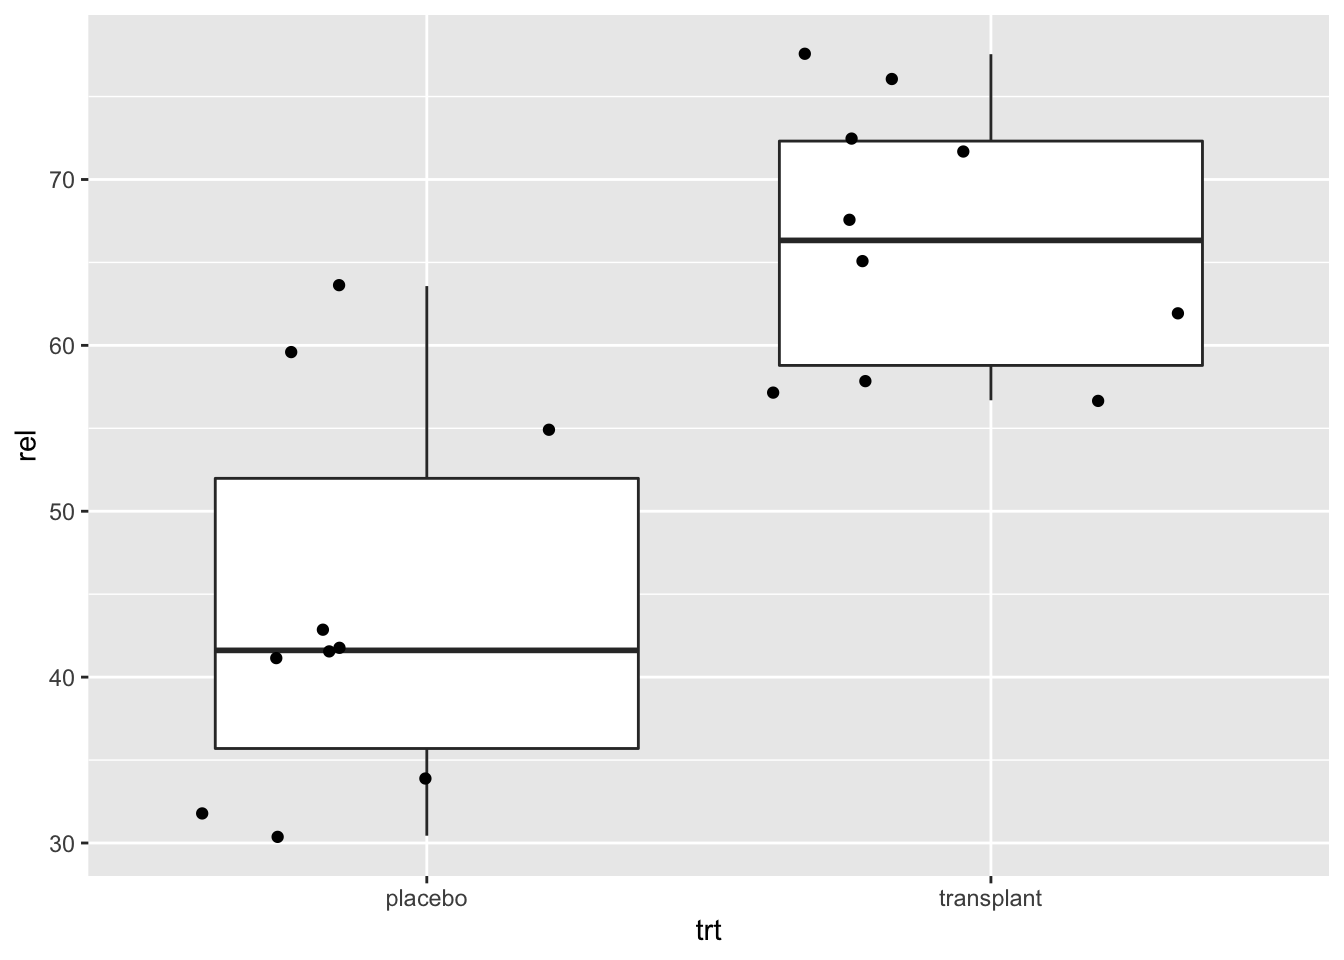
\includegraphics{Statistiek_2020_2021_files/figure-latex/unnamed-chunk-12-1.pdf}

\emph{Interpretatie}

\begin{itemize}
\tightlist
\item
  Zoals we verwachten ligt de verdeling van de lengte van mannen hoger dan deze van vrouwen.
\item
  We zien dat de data min of meer symmetrisch verdeeld zijn in elke groep en een klokvorm hebben.
\item
  We zullen later zien dat de lengte data approximatief normaal verdeeld zijn.
\item
  Dat zal ons toe laten om de data verder samen te vatten door gebruik te maken van twee statistieken: het gemiddelde en de standaard deviatie wat een maat is voor de spreiding van de gegevens rond het gemiddelde.
\end{itemize}

We maken nu een subset van de data die we zullen gebruiken om aan te tonen hoe de variabiliteit in kleine steekproeven kan variëren van steekproef tot steekproef.

\emph{Code}

\begin{enumerate}
\def\labelenumi{\arabic{enumi}.}
\tightlist
\item
  We filteren op leeftijd en verwijderen ontbrekenden gegevens (NA, Not Available).
\item
  We selecteren enkel het geslacht en Lengte zodat de dataset geen onnodige variabelen bevat.
\end{enumerate}

\begin{Shaded}
\begin{Highlighting}[]
\NormalTok{nhanesSub \textless{}{-}}\StringTok{ }\NormalTok{NHANES }\OperatorTok{\%\textgreater{}\%}\StringTok{ }\KeywordTok{filter}\NormalTok{(Age }\OperatorTok{\textgreater{}=}\StringTok{ }\DecValTok{18} \OperatorTok{\&}\StringTok{ }\OperatorTok{!}\KeywordTok{is.na}\NormalTok{(Height)) }\OperatorTok{\%\textgreater{}\%}\StringTok{ }
\StringTok{    }\KeywordTok{select}\NormalTok{(}\KeywordTok{c}\NormalTok{(}\StringTok{"Gender"}\NormalTok{, }\StringTok{"Height"}\NormalTok{))}
\end{Highlighting}
\end{Shaded}

We berekenen het gemiddelde en de standaard deviatie voor de lengte voor mannen en vrouwen in de grote dataset.
We groeperen de data hiervoor op basis van het geslacht (variable Gender).

\begin{Shaded}
\begin{Highlighting}[]
\NormalTok{HeightSum \textless{}{-}}\StringTok{ }\NormalTok{nhanesSub }\OperatorTok{\%\textgreater{}\%}\StringTok{ }\KeywordTok{group\_by}\NormalTok{(Gender) }\OperatorTok{\%\textgreater{}\%}\StringTok{ }\KeywordTok{summarize\_at}\NormalTok{(}\StringTok{"Height"}\NormalTok{, }
    \KeywordTok{list}\NormalTok{(}\DataTypeTok{mean =}\NormalTok{ mean, }\DataTypeTok{sd =}\NormalTok{ sd))}

\NormalTok{knitr}\OperatorTok{::}\KeywordTok{kable}\NormalTok{(HeightSum }\OperatorTok{\%\textgreater{}\%}\StringTok{ }\KeywordTok{mutate\_if}\NormalTok{(is.numeric, round, }
    \DataTypeTok{digits =} \DecValTok{1}\NormalTok{), }\StringTok{"html"}\NormalTok{)}
\end{Highlighting}
\end{Shaded}

Gender

mean

sd

female

162.1

7.3

male

175.9

7.5

\emph{Interpretatie}

Vrouwen zijn gemiddeld 162.1 cm HeightSum en mannen 175.9 cm.
Wat onze intuïtie bevestigt dat mannen gemiddeld groter zijn dan vrouwen.

\hypertarget{experiment}{%
\subsection{Experiment}\label{experiment}}

\begin{itemize}
\item
  Stel dat we geen toegang hebben tot de metingen van de NHANES studie.
\item
  We zouden dan een experiment op moeten zetten om metingen bij mannen en vrouwen te doen.
\item
  Veronderstel dat we budget hebben om metingen bij 5 mannen en 5 vrouwen te doen.
\item
  We zouden dan 5 mannen en 5 vrouwen boven de 25 jaar at random selecteren uit de Amerikaanse populatie.
\item
  We kunnen dit experiment simuleren door 5 vrouwen en 5 mannen at random te selecteren uit de NHANES studie.
\end{itemize}

\emph{Code}

\begin{verbatim}
1. het `set.seed` commando wordt gebruikt omdat we dezelfde steekproef zou trekken als we de code opnieuw laten lopen. Dit is louter om de cursus consistent te houden als we de nota's opnieuw maken.
2. het nSamp object bevat de steekproefgrootte per groep
3. we trekken 5 vrouwelijke subjecten uit de nhanesSub dataset
4. vervolgens trekken we 5 mannen uit de nhanesSub dataset
5. we voegen de data van mannen en vrouwen samen in 1 dataset. Het `rbind` commando zal de data van de rijen onder elkaar zetten.
6. We tonen de dataset
\end{verbatim}

\begin{Shaded}
\begin{Highlighting}[]
\KeywordTok{set.seed}\NormalTok{(}\DecValTok{1023}\NormalTok{)}
\NormalTok{nSamp \textless{}{-}}\StringTok{ }\DecValTok{5}
\NormalTok{fem \textless{}{-}}\StringTok{ }\NormalTok{nhanesSub }\OperatorTok{\%\textgreater{}\%}\StringTok{ }\KeywordTok{filter}\NormalTok{(Gender }\OperatorTok{==}\StringTok{ "female"}\NormalTok{) }\OperatorTok{\%\textgreater{}\%}\StringTok{ }
\StringTok{    }\KeywordTok{sample\_n}\NormalTok{(}\DataTypeTok{size =} \DecValTok{5}\NormalTok{)}

\NormalTok{mal \textless{}{-}}\StringTok{ }\NormalTok{nhanesSub }\OperatorTok{\%\textgreater{}\%}\StringTok{ }\KeywordTok{filter}\NormalTok{(Gender }\OperatorTok{==}\StringTok{ "male"}\NormalTok{) }\OperatorTok{\%\textgreater{}\%}\StringTok{ }\KeywordTok{sample\_n}\NormalTok{(}\DataTypeTok{size =} \DecValTok{5}\NormalTok{)}

\NormalTok{samp1 \textless{}{-}}\StringTok{ }\KeywordTok{rbind}\NormalTok{(fem, mal)}

\NormalTok{samp1}
\end{Highlighting}
\end{Shaded}

\begin{verbatim}
## # A tibble: 10 x 2
##    Gender Height
##    <fct>   <dbl>
##  1 female   164 
##  2 female   160.
##  3 female   159 
##  4 female   154.
##  5 female   156.
##  6 male     170.
##  7 male     183.
##  8 male     183.
##  9 male     185.
## 10 male     170.
\end{verbatim}

We hebben met de code dus een steekproef getrokken van 5 vrouwen en 5 mannen.
We exploreren vervolgens de data in de steekproef.

\emph{Code}

\begin{Shaded}
\begin{Highlighting}[]
\NormalTok{samp1 }\OperatorTok{\%\textgreater{}\%}\StringTok{ }\KeywordTok{ggplot}\NormalTok{(}\KeywordTok{aes}\NormalTok{(}\DataTypeTok{x =}\NormalTok{ Height)) }\OperatorTok{+}\StringTok{ }\KeywordTok{geom\_histogram}\NormalTok{() }\OperatorTok{+}\StringTok{ }
\StringTok{    }\KeywordTok{facet\_grid}\NormalTok{(Gender }\OperatorTok{\textasciitilde{}}\StringTok{ }\NormalTok{.) }\OperatorTok{+}\StringTok{ }\KeywordTok{xlab}\NormalTok{(}\StringTok{"Lengte (cm)"}\NormalTok{)}
\end{Highlighting}
\end{Shaded}

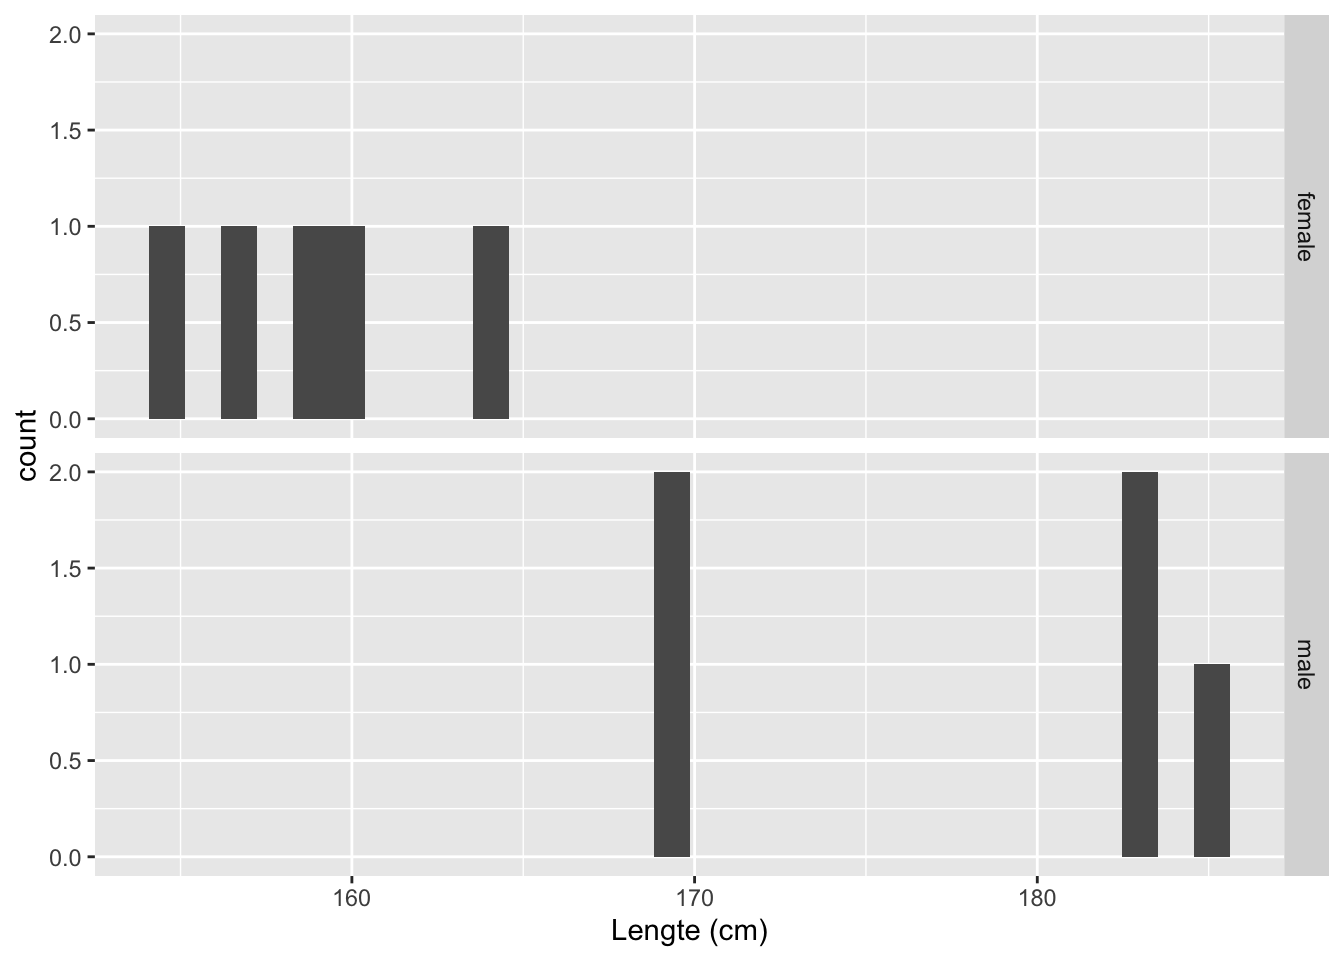
\includegraphics{Statistiek_2020_2021_files/figure-latex/unnamed-chunk-16-1.pdf}

\begin{Shaded}
\begin{Highlighting}[]
\NormalTok{HeightSumExp1 \textless{}{-}}\StringTok{ }\NormalTok{samp1 }\OperatorTok{\%\textgreater{}\%}\StringTok{ }\KeywordTok{group\_by}\NormalTok{(Gender) }\OperatorTok{\%\textgreater{}\%}\StringTok{ }\KeywordTok{summarize\_at}\NormalTok{(}\StringTok{"Height"}\NormalTok{, }
    \KeywordTok{list}\NormalTok{(}\DataTypeTok{mean =}\NormalTok{ mean, }\DataTypeTok{sd =}\NormalTok{ sd))}
\NormalTok{HeightSumExp1}
\end{Highlighting}
\end{Shaded}

\begin{verbatim}
## # A tibble: 2 x 3
##   Gender  mean    sd
##   <fct>  <dbl> <dbl>
## 1 female  159.  3.76
## 2 male    178.  7.55
\end{verbatim}

Histogram is niet zinvol als we maar zo weinig datapunten hebben. Een boxplot is meer geschikt om distributies te vergelijken als er weinig data zijn:

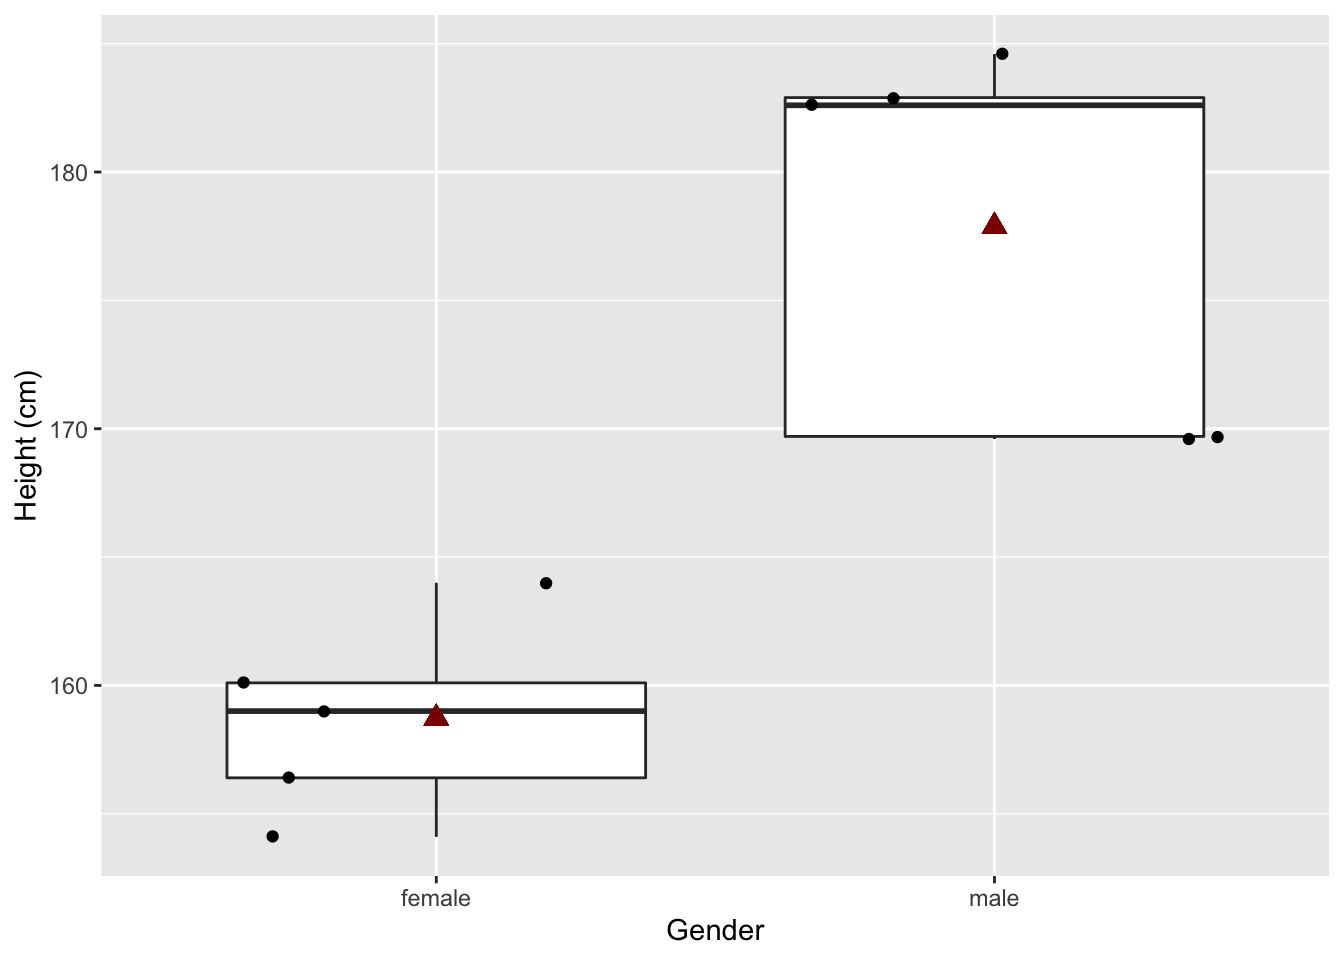
\includegraphics{Statistiek_2020_2021_files/figure-latex/unnamed-chunk-17-1.pdf}

\emph{Einde Code}

Om na te gaan of het verschil in de steekproef groot genoeg is om de bevindingen van de steekproef te kunnen veralgemenen naar de populatie toe voeren we opnieuw een t-test uit.

Met de p-waarde wordt de kans berekend om in een nieuwe random steekproef door toeval een effect te vinden dat in absolute waarde minstens evengroot is als in onze geobserveerde steekproef onder de aanname dat er in werkelijkheid geen verschil zou zijn in gemiddelde lengte tussen vrouwen en mannen.

Als die kans heel klein is is het weinig waarschijnlijk om onze steekproef te observeren onder de hypothese dat de lengtes gemiddeld niet verschillen tussen vrouwen en mannen en kunnen we deze hypothese verwerpen.

Typisch wordt de kans op een valse positieve conclusie gecontroleerd op 5\%.

\begin{Shaded}
\begin{Highlighting}[]
\KeywordTok{t.test}\NormalTok{(Height }\OperatorTok{\textasciitilde{}}\StringTok{ }\NormalTok{Gender, }\DataTypeTok{data =}\NormalTok{ samp1)}
\end{Highlighting}
\end{Shaded}

\begin{verbatim}
## 
##  Welch Two Sample t-test
## 
## data:  Height by Gender
## t = -5.0783, df = 5.8695, p-value = 0.00242
## alternative hypothesis: true difference in means is not equal to 0
## 95 percent confidence interval:
##  -28.441927  -9.878073
## sample estimates:
## mean in group female   mean in group male 
##               158.72               177.88
\end{verbatim}

In het experiment zijn vrouwen gemiddeld 19.16 cm kleiner dan mannen. En als we een statistische test uitvoeren (zie hoofdstuk 5: Statistische besluitvorming) kunnen we besluiten dat dit verschil statistisch significant is.

\hypertarget{herhaal-het-experiment}{%
\subsection{Herhaal het experiment}\label{herhaal-het-experiment}}

Als we het experiment herhalen selecteren we andere mensen en verkrijgen we andere resultaten.

\begin{Shaded}
\begin{Highlighting}[]
\KeywordTok{set.seed}\NormalTok{(}\DecValTok{1024}\NormalTok{)}
\NormalTok{fem \textless{}{-}}\StringTok{ }\NormalTok{nhanesSub }\OperatorTok{\%\textgreater{}\%}\StringTok{ }\KeywordTok{filter}\NormalTok{(Gender }\OperatorTok{==}\StringTok{ "female"}\NormalTok{) }\OperatorTok{\%\textgreater{}\%}\StringTok{ }
\StringTok{    }\KeywordTok{sample\_n}\NormalTok{(}\DataTypeTok{size =} \DecValTok{5}\NormalTok{)}

\NormalTok{mal \textless{}{-}}\StringTok{ }\NormalTok{nhanesSub }\OperatorTok{\%\textgreater{}\%}\StringTok{ }\KeywordTok{filter}\NormalTok{(Gender }\OperatorTok{==}\StringTok{ "male"}\NormalTok{) }\OperatorTok{\%\textgreater{}\%}\StringTok{ }\KeywordTok{sample\_n}\NormalTok{(}\DataTypeTok{size =} \DecValTok{5}\NormalTok{)}

\NormalTok{samp2 \textless{}{-}}\StringTok{ }\KeywordTok{rbind}\NormalTok{(fem, mal)}

\NormalTok{HeightSumExp2 \textless{}{-}}\StringTok{ }\NormalTok{samp2 }\OperatorTok{\%\textgreater{}\%}\StringTok{ }\KeywordTok{group\_by}\NormalTok{(Gender) }\OperatorTok{\%\textgreater{}\%}\StringTok{ }\KeywordTok{summarize\_at}\NormalTok{(}\StringTok{"Height"}\NormalTok{, }
    \KeywordTok{list}\NormalTok{(}\DataTypeTok{mean =}\NormalTok{ mean, }\DataTypeTok{sd =}\NormalTok{ sd))}
\NormalTok{HeightSumExp2}
\end{Highlighting}
\end{Shaded}

\begin{verbatim}
## # A tibble: 2 x 3
##   Gender  mean    sd
##   <fct>  <dbl> <dbl>
## 1 female  166.  9.89
## 2 male    170.  8.24
\end{verbatim}

\begin{Shaded}
\begin{Highlighting}[]
\NormalTok{samp2 }\OperatorTok{\%\textgreater{}\%}\StringTok{ }\KeywordTok{ggplot}\NormalTok{(}\KeywordTok{aes}\NormalTok{(}\DataTypeTok{x =}\NormalTok{ Gender, }\DataTypeTok{y =}\NormalTok{ Height)) }\OperatorTok{+}\StringTok{ }\KeywordTok{geom\_boxplot}\NormalTok{(}\DataTypeTok{outlier.shape =} \OtherTok{NA}\NormalTok{) }\OperatorTok{+}\StringTok{ }
\StringTok{    }\KeywordTok{geom\_point}\NormalTok{(}\DataTypeTok{position =} \StringTok{"jitter"}\NormalTok{) }\OperatorTok{+}\StringTok{ }\KeywordTok{geom\_point}\NormalTok{(}\KeywordTok{aes}\NormalTok{(}\DataTypeTok{x =} \DecValTok{1}\NormalTok{, }
    \DataTypeTok{y =}\NormalTok{ HeightSumExp2}\OperatorTok{$}\NormalTok{mean[}\DecValTok{1}\NormalTok{]), }\DataTypeTok{size =} \DecValTok{3}\NormalTok{, }\DataTypeTok{pch =} \DecValTok{17}\NormalTok{, }
    \DataTypeTok{color =} \StringTok{"darkred"}\NormalTok{) }\OperatorTok{+}\StringTok{ }\KeywordTok{geom\_point}\NormalTok{(}\KeywordTok{aes}\NormalTok{(}\DataTypeTok{x =} \DecValTok{2}\NormalTok{, }\DataTypeTok{y =}\NormalTok{ HeightSumExp2}\OperatorTok{$}\NormalTok{mean[}\DecValTok{2}\NormalTok{]), }
    \DataTypeTok{size =} \DecValTok{3}\NormalTok{, }\DataTypeTok{pch =} \DecValTok{17}\NormalTok{, }\DataTypeTok{color =} \StringTok{"darkred"}\NormalTok{) }\OperatorTok{+}\StringTok{ }\KeywordTok{ylab}\NormalTok{(}\StringTok{"Height (cm)"}\NormalTok{)}
\end{Highlighting}
\end{Shaded}

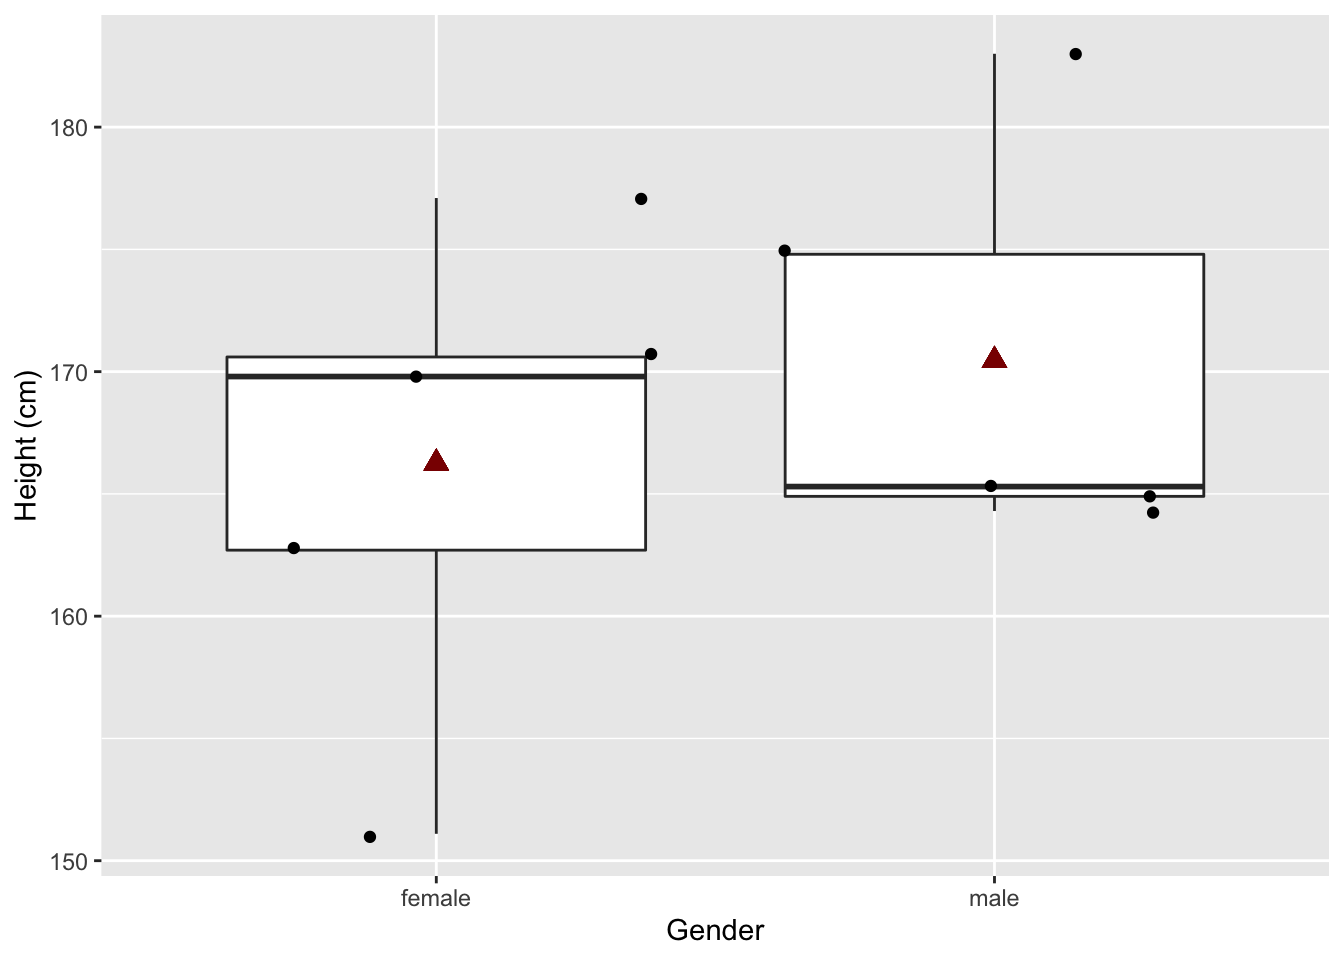
\includegraphics{Statistiek_2020_2021_files/figure-latex/unnamed-chunk-19-1.pdf}

\begin{Shaded}
\begin{Highlighting}[]
\KeywordTok{t.test}\NormalTok{(Height }\OperatorTok{\textasciitilde{}}\StringTok{ }\NormalTok{Gender, }\DataTypeTok{data =}\NormalTok{ samp2)}
\end{Highlighting}
\end{Shaded}

\begin{verbatim}
## 
##  Welch Two Sample t-test
## 
## data:  Height by Gender
## t = -0.7295, df = 7.747, p-value = 0.4872
## alternative hypothesis: true difference in means is not equal to 0
## 95 percent confidence interval:
##  -17.552343   9.152343
## sample estimates:
## mean in group female   mean in group male 
##               166.26               170.46
\end{verbatim}

Vijf andere mannen en vrouwen worden getrokken uit de populatie. Hierdoor verschillen de lengte metingen van de vorige steekproef alsook de berekende gemiddeldes en de p-waarde van de statistische toets.

In de nieuwe steekproef zijn vrouwen gemiddeld 4.2 cm kleiner dan mannen. En dit verschil is statistisch niet significant

\hypertarget{herhaal-het-experiment-opnieuw}{%
\subsection{Herhaal het experiment opnieuw}\label{herhaal-het-experiment-opnieuw}}

\begin{Shaded}
\begin{Highlighting}[]
\NormalTok{seed \textless{}{-}}\StringTok{ }\DecValTok{88605}
\KeywordTok{set.seed}\NormalTok{(seed)}
\NormalTok{fem \textless{}{-}}\StringTok{ }\NormalTok{nhanesSub }\OperatorTok{\%\textgreater{}\%}\StringTok{ }\KeywordTok{filter}\NormalTok{(Gender }\OperatorTok{==}\StringTok{ "female"}\NormalTok{) }\OperatorTok{\%\textgreater{}\%}\StringTok{ }
\StringTok{    }\KeywordTok{sample\_n}\NormalTok{(}\DataTypeTok{size =} \DecValTok{5}\NormalTok{)}

\NormalTok{mal \textless{}{-}}\StringTok{ }\NormalTok{nhanesSub }\OperatorTok{\%\textgreater{}\%}\StringTok{ }\KeywordTok{filter}\NormalTok{(Gender }\OperatorTok{==}\StringTok{ "male"}\NormalTok{) }\OperatorTok{\%\textgreater{}\%}\StringTok{ }\KeywordTok{sample\_n}\NormalTok{(}\DataTypeTok{size =} \DecValTok{5}\NormalTok{)}

\NormalTok{samp3 \textless{}{-}}\StringTok{ }\KeywordTok{rbind}\NormalTok{(fem, mal)}

\NormalTok{HeightSumExp3 \textless{}{-}}\StringTok{ }\NormalTok{samp3 }\OperatorTok{\%\textgreater{}\%}\StringTok{ }\KeywordTok{group\_by}\NormalTok{(Gender) }\OperatorTok{\%\textgreater{}\%}\StringTok{ }\KeywordTok{summarize\_at}\NormalTok{(}\StringTok{"Height"}\NormalTok{, }
    \KeywordTok{list}\NormalTok{(}\DataTypeTok{mean =}\NormalTok{ mean, }\DataTypeTok{sd =}\NormalTok{ sd))}
\NormalTok{HeightSumExp3}
\end{Highlighting}
\end{Shaded}

\begin{verbatim}
## # A tibble: 2 x 3
##   Gender  mean    sd
##   <fct>  <dbl> <dbl>
## 1 female  173.  1.97
## 2 male    168.  2.84
\end{verbatim}

\begin{Shaded}
\begin{Highlighting}[]
\NormalTok{samp3 }\OperatorTok{\%\textgreater{}\%}\StringTok{ }\KeywordTok{ggplot}\NormalTok{(}\KeywordTok{aes}\NormalTok{(}\DataTypeTok{x =}\NormalTok{ Gender, }\DataTypeTok{y =}\NormalTok{ Height)) }\OperatorTok{+}\StringTok{ }\KeywordTok{geom\_boxplot}\NormalTok{(}\DataTypeTok{outlier.shape =} \OtherTok{NA}\NormalTok{) }\OperatorTok{+}\StringTok{ }
\StringTok{    }\KeywordTok{geom\_point}\NormalTok{(}\DataTypeTok{position =} \StringTok{"jitter"}\NormalTok{) }\OperatorTok{+}\StringTok{ }\KeywordTok{geom\_point}\NormalTok{(}\KeywordTok{aes}\NormalTok{(}\DataTypeTok{x =} \DecValTok{1}\NormalTok{, }
    \DataTypeTok{y =}\NormalTok{ HeightSumExp3}\OperatorTok{$}\NormalTok{mean[}\DecValTok{1}\NormalTok{]), }\DataTypeTok{size =} \DecValTok{3}\NormalTok{, }\DataTypeTok{pch =} \DecValTok{17}\NormalTok{, }
    \DataTypeTok{color =} \StringTok{"darkred"}\NormalTok{) }\OperatorTok{+}\StringTok{ }\KeywordTok{geom\_point}\NormalTok{(}\KeywordTok{aes}\NormalTok{(}\DataTypeTok{x =} \DecValTok{2}\NormalTok{, }\DataTypeTok{y =}\NormalTok{ HeightSumExp3}\OperatorTok{$}\NormalTok{mean[}\DecValTok{2}\NormalTok{]), }
    \DataTypeTok{size =} \DecValTok{3}\NormalTok{, }\DataTypeTok{pch =} \DecValTok{17}\NormalTok{, }\DataTypeTok{color =} \StringTok{"darkred"}\NormalTok{) }\OperatorTok{+}\StringTok{ }\KeywordTok{ylab}\NormalTok{(}\StringTok{"Height (cm)"}\NormalTok{)}
\end{Highlighting}
\end{Shaded}

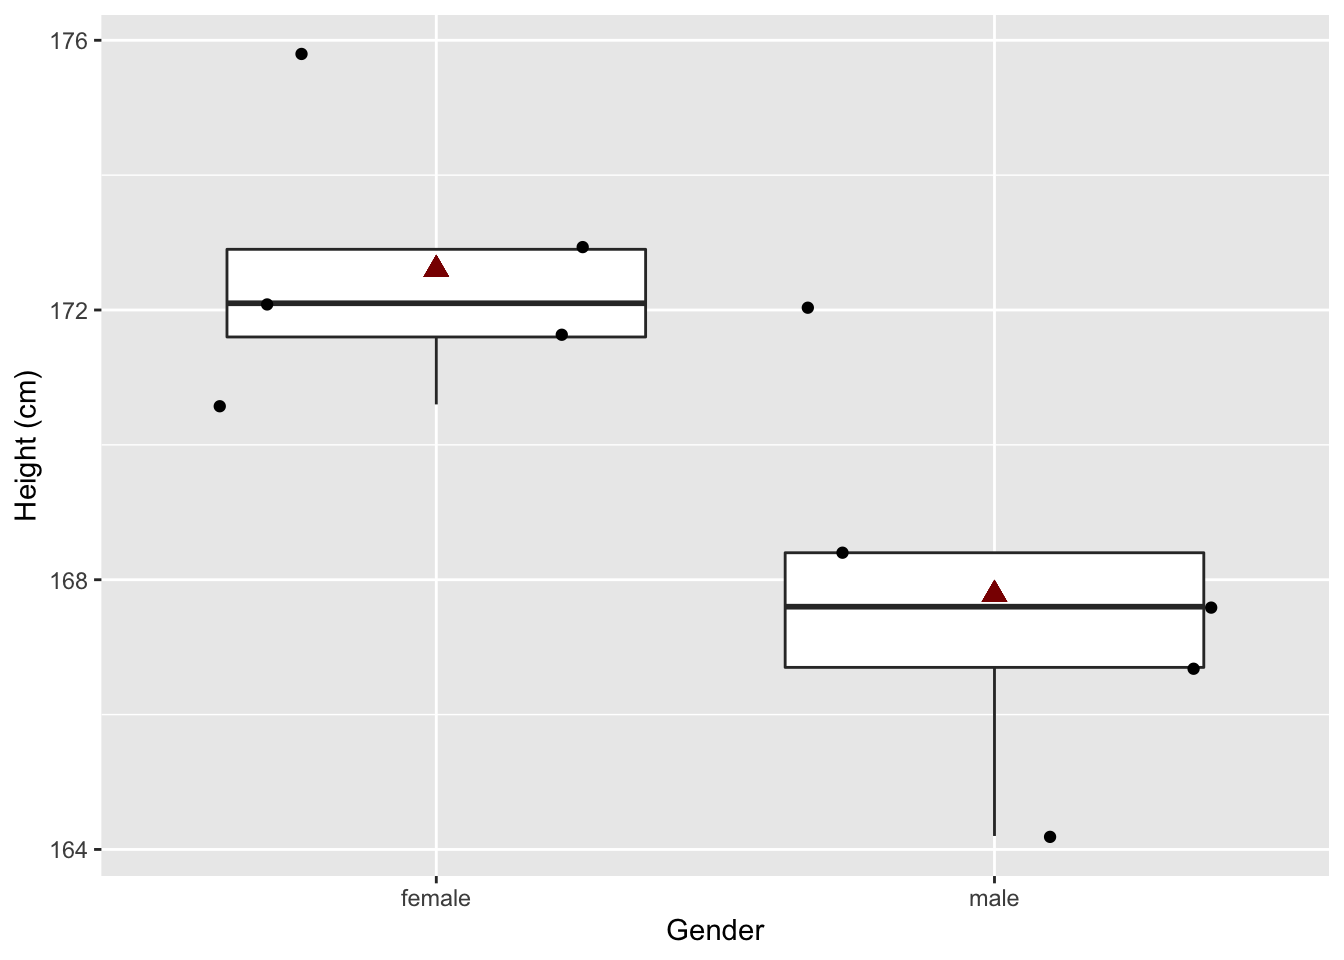
\includegraphics{Statistiek_2020_2021_files/figure-latex/unnamed-chunk-20-1.pdf}

\begin{Shaded}
\begin{Highlighting}[]
\KeywordTok{t.test}\NormalTok{(Height }\OperatorTok{\textasciitilde{}}\StringTok{ }\NormalTok{Gender, }\DataTypeTok{data =}\NormalTok{ samp3)}
\end{Highlighting}
\end{Shaded}

\begin{verbatim}
## 
##  Welch Two Sample t-test
## 
## data:  Height by Gender
## t = 3.1182, df = 7.136, p-value = 0.01648
## alternative hypothesis: true difference in means is not equal to 0
## 95 percent confidence interval:
##  1.178916 8.461084
## sample estimates:
## mean in group female   mean in group male 
##               172.60               167.78
\end{verbatim}

In de nieuwe steekproef zijn vrouwen gemiddeld 4.82 cm groter dan mannen. En dit verschil is statistisch significant

Merk op dat we in deze extreme steekproef door toeval vrij grote vrouwen en eerder kleine mannen hebben getrokken uit de populatie. Een dergelijke steekproef zal eerder zeldzaam zijn maar kan door toeval voorkomen.

In de onderstaande paragraaf leggen we uit hoe we deze extreme steekproef hebben bekomen:

Een seed wordt in de cursus gebruikt om ervoor te zorgen dat we telkens dezelfde resultaten bekomen als we de random generator opnieuw laten lopen in R (zie het set.seed commando). Dat doen we puur om de resultaten in de cursus gelijk te kunnen houden als we aanpassingen hebben doorgevoerd aan de tekst en de code dus opnieuw moeten laten lopen om de cursus te compileren. In vrijwel alle code is de seed gewoon random gekozen.

Om de extreme steekproef weer te geven, hebben we deze keer echter geen random seed gebruikt. Daarvoor hebben we alle seeds overlopen van 1 tot 100000. We hebben dus \ensuremath{8.8605\times 10^{4}} steekproeven moeten trekken alvorens we een dergelijke extreme steekproef uit de populatie hadden getrokken waaruit we ten onrechte zouden concluderen dat vrouwen gemiddeld significant groter zijn dan mannen.

\hypertarget{samenvatting}{%
\subsection{Samenvatting}\label{samenvatting}}

We trokken at random andere proefpersonen in elke steekproef. Hierdoor

\begin{itemize}
\item
  verschillen de lengtemetingen van steekproef tot steekproef.
\item
  Dus ook de geschatte gemiddeldes en standaard deviaties.
\item
  Bijgevolg zijn onze conclusies ook onzeker en kunnen deze wijzigen van steekproef tot steekproef.
\item
  Ook steekproeven waarbij het effect tegengesteld is aan dat in de populatie en waarbij we besluiten dat het verschil significant is kunnen voorkomen.
\item
  We kunnen aantonen dat dergelijke steekproeven voor experimenten waarbij we de lengte tussen mannen en vrouwen vergelijken eerder zeldzaam zijn.
\end{itemize}

\(\rightarrow\) Met statistiek gaan we de kans op het trekken foute conclusies controleren.

\hypertarget{controle-van-beslissingsfouten}{%
\subsection{Controle van beslissingsfouten}\label{controle-van-beslissingsfouten}}

Hoe controleert statistiek de kans op het trekken van foute conclusies?

\begin{itemize}
\tightlist
\item
  In onderstaande code trekken we 10000 herhaalde steekproeven van 5 vrouwen en 5 mannen uit de NHANES studie.
\end{itemize}

\emph{Code}

Deze code is vrij complex. Het kan nuttig zijn om deze pas na de twee modules Introductie tot R, en, data visualisatie opnieuw te bekijken.

\begin{Shaded}
\begin{Highlighting}[]
\KeywordTok{set.seed}\NormalTok{(}\DecValTok{15152}\NormalTok{)}
\CommentTok{\# Aantal simulaties en steekproefgrootte per groep}
\NormalTok{nSim \textless{}{-}}\StringTok{ }\DecValTok{10000}
\NormalTok{nSamp \textless{}{-}}\StringTok{ }\DecValTok{5}

\CommentTok{\# We filteren de data vooraf zodat we dit niet}
\CommentTok{\# telkens opnieuw hoeven te doen}
\NormalTok{fem \textless{}{-}}\StringTok{ }\NormalTok{nhanesSub }\OperatorTok{\%\textgreater{}\%}\StringTok{ }\KeywordTok{filter}\NormalTok{(Gender }\OperatorTok{==}\StringTok{ "female"}\NormalTok{)}

\NormalTok{mal \textless{}{-}}\StringTok{ }\NormalTok{nhanesSub }\OperatorTok{\%\textgreater{}\%}\StringTok{ }\KeywordTok{filter}\NormalTok{(Gender }\OperatorTok{==}\StringTok{ "male"}\NormalTok{)}

\CommentTok{\# Simulatie studie Om snelle functies te kunnen}
\CommentTok{\# gebruiken nemen we eerst nSim steekproeven en}
\CommentTok{\# berekenen we daarna alles.}

\NormalTok{femSamps \textless{}{-}}\StringTok{ }\NormalTok{malSamps \textless{}{-}}\StringTok{ }\KeywordTok{matrix}\NormalTok{(}\OtherTok{NA}\NormalTok{, }\DataTypeTok{nrow =}\NormalTok{ nSamp, }\DataTypeTok{ncol =}\NormalTok{ nSim)}
\ControlFlowTok{for}\NormalTok{ (i }\ControlFlowTok{in} \DecValTok{1}\OperatorTok{:}\NormalTok{nSim) \{}
\NormalTok{    femSamps[, i] \textless{}{-}}\StringTok{ }\KeywordTok{sample}\NormalTok{(fem}\OperatorTok{$}\NormalTok{Height, nSamp)}
\NormalTok{    malSamps[, i] \textless{}{-}}\StringTok{ }\KeywordTok{sample}\NormalTok{(mal}\OperatorTok{$}\NormalTok{Height, nSamp)}
\NormalTok{\}}

\NormalTok{res \textless{}{-}}\StringTok{ }\KeywordTok{data.frame}\NormalTok{(}\DataTypeTok{verschil =} \KeywordTok{colMeans}\NormalTok{(femSamps) }\OperatorTok{{-}}\StringTok{ }\KeywordTok{colMeans}\NormalTok{(malSamps), }
\NormalTok{    Rfast}\OperatorTok{::}\KeywordTok{ttests}\NormalTok{(femSamps, malSamps))}

\KeywordTok{sum}\NormalTok{(res}\OperatorTok{$}\NormalTok{pvalue }\OperatorTok{\textless{}}\StringTok{ }\FloatTok{0.05} \OperatorTok{\&}\StringTok{ }\NormalTok{res}\OperatorTok{$}\NormalTok{verschil }\OperatorTok{\textless{}}\StringTok{ }\DecValTok{0}\NormalTok{)}
\end{Highlighting}
\end{Shaded}

\begin{verbatim}
## [1] 7234
\end{verbatim}

\begin{Shaded}
\begin{Highlighting}[]
\KeywordTok{sum}\NormalTok{(res}\OperatorTok{$}\NormalTok{pvalue }\OperatorTok{\textgreater{}=}\StringTok{ }\FloatTok{0.05}\NormalTok{)}
\end{Highlighting}
\end{Shaded}

\begin{verbatim}
## [1] 2766
\end{verbatim}

\begin{Shaded}
\begin{Highlighting}[]
\KeywordTok{sum}\NormalTok{(res}\OperatorTok{$}\NormalTok{pvalue }\OperatorTok{\textless{}}\StringTok{ }\FloatTok{0.05} \OperatorTok{\&}\StringTok{ }\NormalTok{res}\OperatorTok{$}\NormalTok{verschil }\OperatorTok{\textgreater{}}\StringTok{ }\DecValTok{0}\NormalTok{)}
\end{Highlighting}
\end{Shaded}

\begin{verbatim}
## [1] 0
\end{verbatim}

\begin{Shaded}
\begin{Highlighting}[]
\NormalTok{res }\OperatorTok{\%\textgreater{}\%}\StringTok{ }\KeywordTok{ggplot}\NormalTok{(}\KeywordTok{aes}\NormalTok{(}\DataTypeTok{x =}\NormalTok{ verschil, }\DataTypeTok{y =} \OperatorTok{{-}}\KeywordTok{log10}\NormalTok{(pvalue), }
    \DataTypeTok{color =}\NormalTok{ pvalue }\OperatorTok{\textless{}}\StringTok{ }\FloatTok{0.05}\NormalTok{)) }\OperatorTok{+}\StringTok{ }\KeywordTok{geom\_point}\NormalTok{() }\OperatorTok{+}\StringTok{ }\KeywordTok{xlab}\NormalTok{(}\StringTok{"Gemiddeld Verschil (cm)"}\NormalTok{) }\OperatorTok{+}\StringTok{ }
\StringTok{    }\KeywordTok{ylab}\NormalTok{(}\StringTok{"Statistische Significantie ({-}log10 p)"}\NormalTok{)}
\end{Highlighting}
\end{Shaded}

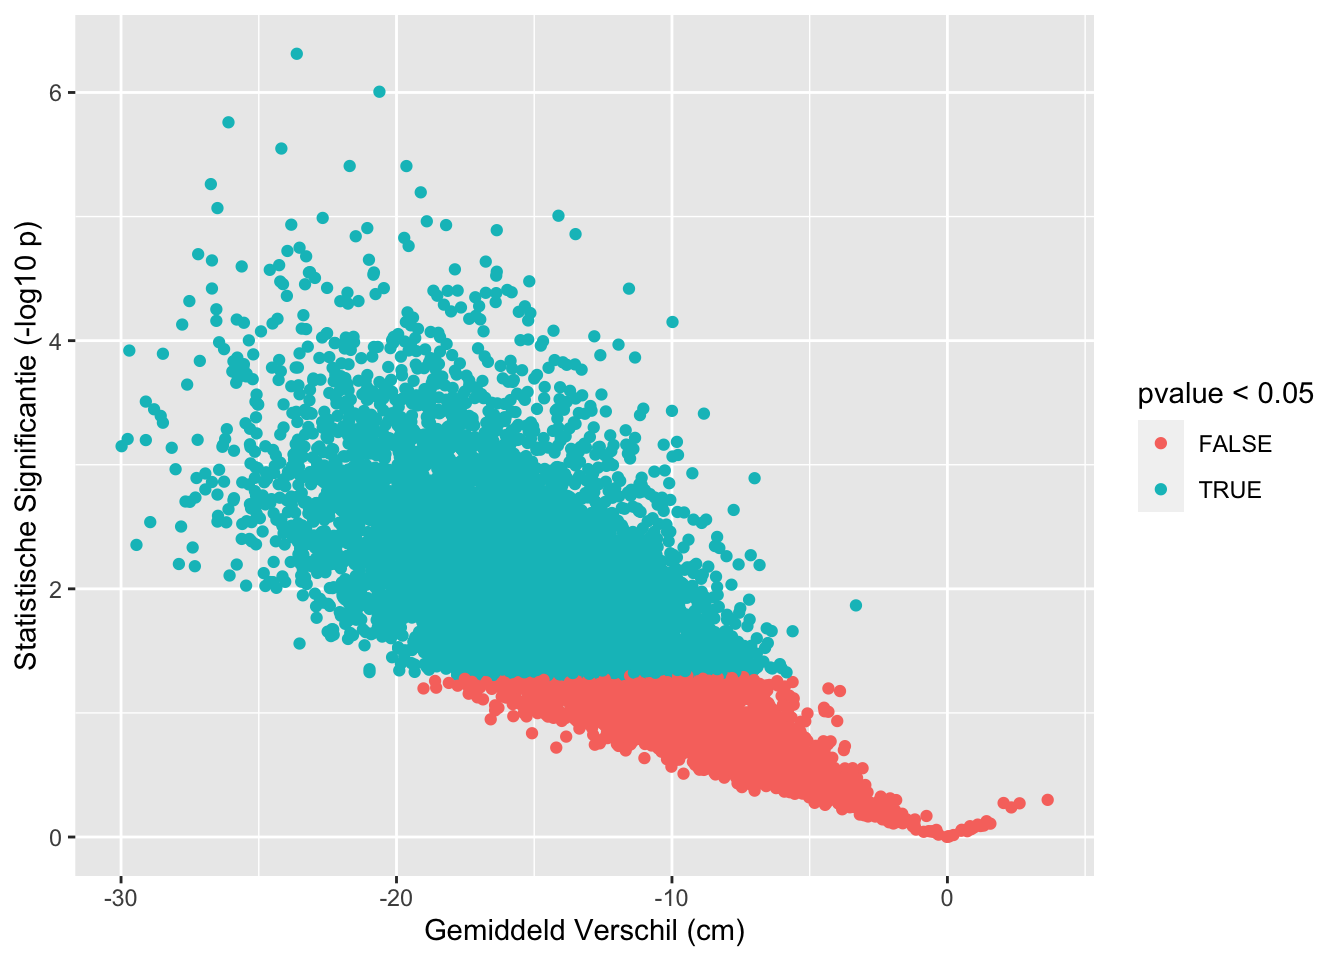
\includegraphics{Statistiek_2020_2021_files/figure-latex/unnamed-chunk-21-1.pdf}

\begin{Shaded}
\begin{Highlighting}[]
\NormalTok{res }\OperatorTok{\%\textgreater{}\%}\StringTok{ }\KeywordTok{ggplot}\NormalTok{(}\KeywordTok{aes}\NormalTok{(}\DataTypeTok{y =}\NormalTok{ verschil)) }\OperatorTok{+}\StringTok{ }\KeywordTok{geom\_boxplot}\NormalTok{() }\OperatorTok{+}\StringTok{ }
\StringTok{    }\KeywordTok{ylab}\NormalTok{(}\StringTok{"Gemiddeld Verschil (cm)"}\NormalTok{)}
\end{Highlighting}
\end{Shaded}

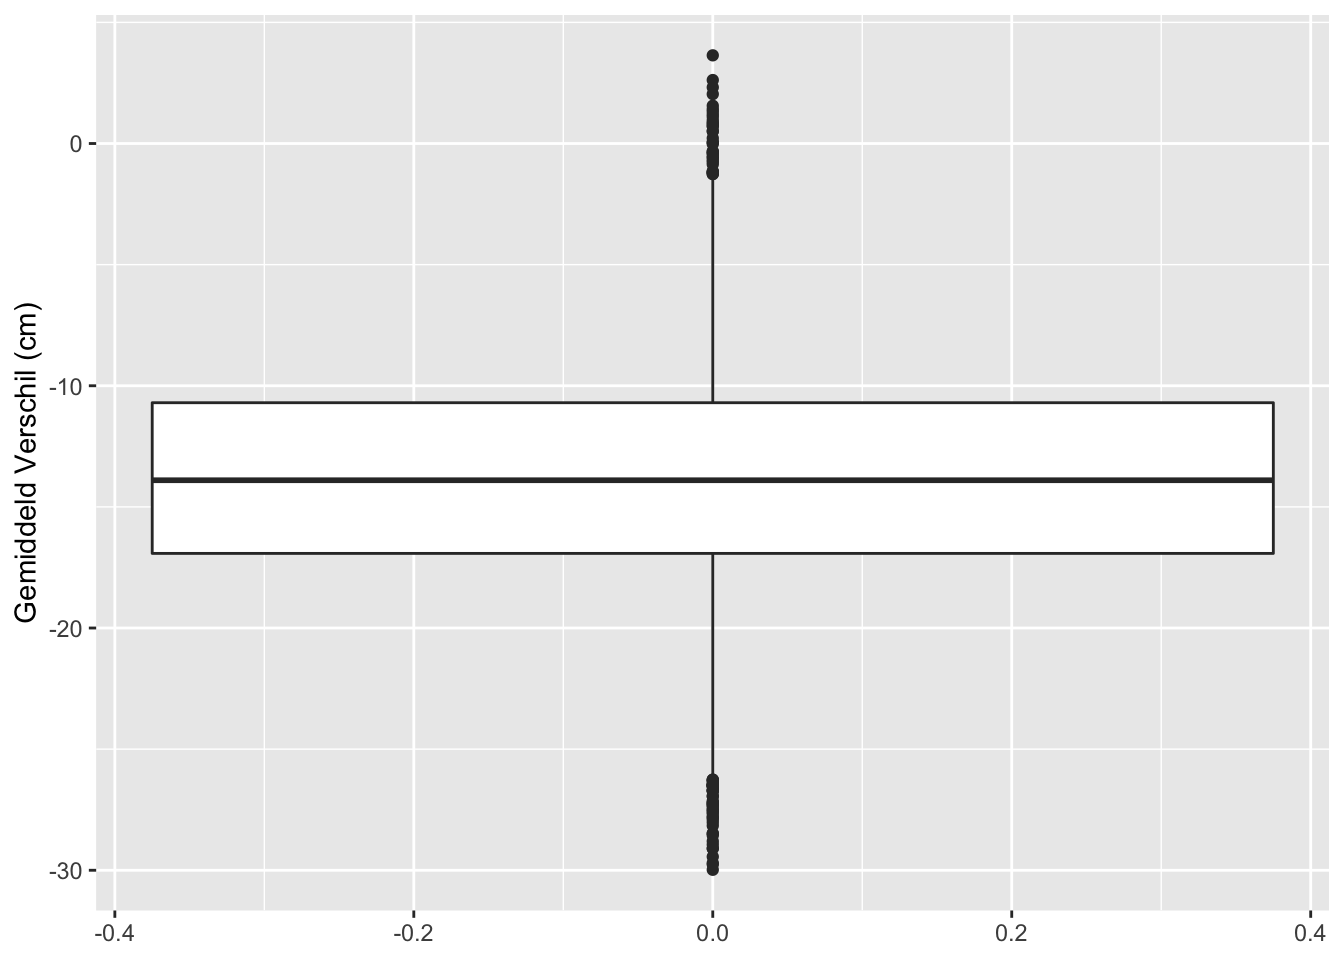
\includegraphics{Statistiek_2020_2021_files/figure-latex/unnamed-chunk-21-2.pdf}

\begin{Shaded}
\begin{Highlighting}[]
\KeywordTok{xlab}\NormalTok{(}\StringTok{""}\NormalTok{)}
\end{Highlighting}
\end{Shaded}

\begin{verbatim}
## $x
## [1] ""
## 
## attr(,"class")
## [1] "labels"
\end{verbatim}

Op basis van 10000 steekproeven van 5 mannen en 5 vrouwen zagen we dat in 7234 steekproeven vrouwen gemiddeld significant kleiner zijn dan mannen. In 2766 steekproeven besluiten we dat vrouwen en mannen gemiddeld niet significant verschillen in lengte. En in 0 besluiten we dat vrouwen gemiddeld significant groter zijn dan mannen.

\begin{itemize}
\item
  De steekproef die we toonden waaruit we zouden besluiten dat vrouwen significant groter zijn dan mannen is heel onwaarschijnlijk. Er moesten 88605 steekproeven worden getrokken om deze extreme steekproef te vinden.
\item
  Het feit dat we in veel steekproeven resultaten vinden die statistisch niet significant zijn komt omdat de statistische toets een te lage kracht heeft om het verschil te detecteren wanneer er maar 5 observaties zijn per groep.
\end{itemize}

\begin{center}\rule{0.5\linewidth}{0.5pt}\end{center}

\hypertarget{grotere-steekproef}{%
\subsubsection{Grotere steekproef?}\label{grotere-steekproef}}

Wat gebeurt er als we de steekproef verhogen naar 50 observaties per groep?

\begin{Shaded}
\begin{Highlighting}[]
\KeywordTok{set.seed}\NormalTok{(}\DecValTok{11145}\NormalTok{)}
\CommentTok{\# Aantal simulaties en steekproefgrootte per groep}
\NormalTok{nSim \textless{}{-}}\StringTok{ }\DecValTok{10000}
\NormalTok{nSamp \textless{}{-}}\StringTok{ }\DecValTok{50}

\CommentTok{\# We filteren de data vooraf zodat we dit niet}
\CommentTok{\# telkens opnieuw hoeven te doen}
\NormalTok{fem \textless{}{-}}\StringTok{ }\NormalTok{nhanesSub }\OperatorTok{\%\textgreater{}\%}\StringTok{ }\KeywordTok{filter}\NormalTok{(Gender }\OperatorTok{==}\StringTok{ "female"}\NormalTok{)}

\NormalTok{mal \textless{}{-}}\StringTok{ }\NormalTok{nhanesSub }\OperatorTok{\%\textgreater{}\%}\StringTok{ }\KeywordTok{filter}\NormalTok{(Gender }\OperatorTok{==}\StringTok{ "male"}\NormalTok{)}

\CommentTok{\# Simulatie studie Om snelle functies te kunnen}
\CommentTok{\# gebruiken nemen we eerst nSim steekproeven en}
\CommentTok{\# berekenen we daarna alles.}

\NormalTok{femSamps \textless{}{-}}\StringTok{ }\NormalTok{malSamps \textless{}{-}}\StringTok{ }\KeywordTok{matrix}\NormalTok{(}\OtherTok{NA}\NormalTok{, }\DataTypeTok{nrow =}\NormalTok{ nSamp, }\DataTypeTok{ncol =}\NormalTok{ nSim)}
\ControlFlowTok{for}\NormalTok{ (i }\ControlFlowTok{in} \DecValTok{1}\OperatorTok{:}\NormalTok{nSim) \{}
\NormalTok{    femSamps[, i] \textless{}{-}}\StringTok{ }\KeywordTok{sample}\NormalTok{(fem}\OperatorTok{$}\NormalTok{Height, nSamp)}
\NormalTok{    malSamps[, i] \textless{}{-}}\StringTok{ }\KeywordTok{sample}\NormalTok{(mal}\OperatorTok{$}\NormalTok{Height, nSamp)}
\NormalTok{\}}

\NormalTok{res \textless{}{-}}\StringTok{ }\KeywordTok{data.frame}\NormalTok{(}\DataTypeTok{verschil =} \KeywordTok{colMeans}\NormalTok{(femSamps) }\OperatorTok{{-}}\StringTok{ }\KeywordTok{colMeans}\NormalTok{(malSamps), }
\NormalTok{    Rfast}\OperatorTok{::}\KeywordTok{ttests}\NormalTok{(femSamps, malSamps))}

\KeywordTok{sum}\NormalTok{(res}\OperatorTok{$}\NormalTok{pvalue }\OperatorTok{\textless{}}\StringTok{ }\FloatTok{0.05} \OperatorTok{\&}\StringTok{ }\NormalTok{res}\OperatorTok{$}\NormalTok{verschil }\OperatorTok{\textless{}}\StringTok{ }\DecValTok{0}\NormalTok{)}
\end{Highlighting}
\end{Shaded}

\begin{verbatim}
## [1] 10000
\end{verbatim}

\begin{Shaded}
\begin{Highlighting}[]
\KeywordTok{sum}\NormalTok{(res}\OperatorTok{$}\NormalTok{pvalue }\OperatorTok{\textgreater{}=}\StringTok{ }\FloatTok{0.05}\NormalTok{)}
\end{Highlighting}
\end{Shaded}

\begin{verbatim}
## [1] 0
\end{verbatim}

\begin{Shaded}
\begin{Highlighting}[]
\KeywordTok{sum}\NormalTok{(res}\OperatorTok{$}\NormalTok{pvalue }\OperatorTok{\textless{}}\StringTok{ }\FloatTok{0.05} \OperatorTok{\&}\StringTok{ }\NormalTok{res}\OperatorTok{$}\NormalTok{verschil }\OperatorTok{\textgreater{}}\StringTok{ }\DecValTok{0}\NormalTok{)}
\end{Highlighting}
\end{Shaded}

\begin{verbatim}
## [1] 0
\end{verbatim}

\begin{Shaded}
\begin{Highlighting}[]
\NormalTok{res }\OperatorTok{\%\textgreater{}\%}\StringTok{ }\KeywordTok{ggplot}\NormalTok{(}\KeywordTok{aes}\NormalTok{(}\DataTypeTok{x =}\NormalTok{ verschil, }\DataTypeTok{y =} \OperatorTok{{-}}\KeywordTok{log10}\NormalTok{(pvalue), }
    \DataTypeTok{color =}\NormalTok{ pvalue }\OperatorTok{\textless{}}\StringTok{ }\FloatTok{0.05}\NormalTok{)) }\OperatorTok{+}\StringTok{ }\KeywordTok{geom\_point}\NormalTok{() }\OperatorTok{+}\StringTok{ }\KeywordTok{xlab}\NormalTok{(}\StringTok{"Gemiddeld Verschil (cm)"}\NormalTok{) }\OperatorTok{+}\StringTok{ }
\StringTok{    }\KeywordTok{ylab}\NormalTok{(}\StringTok{"Statistische Significantie ({-}log10 p)"}\NormalTok{)}
\end{Highlighting}
\end{Shaded}

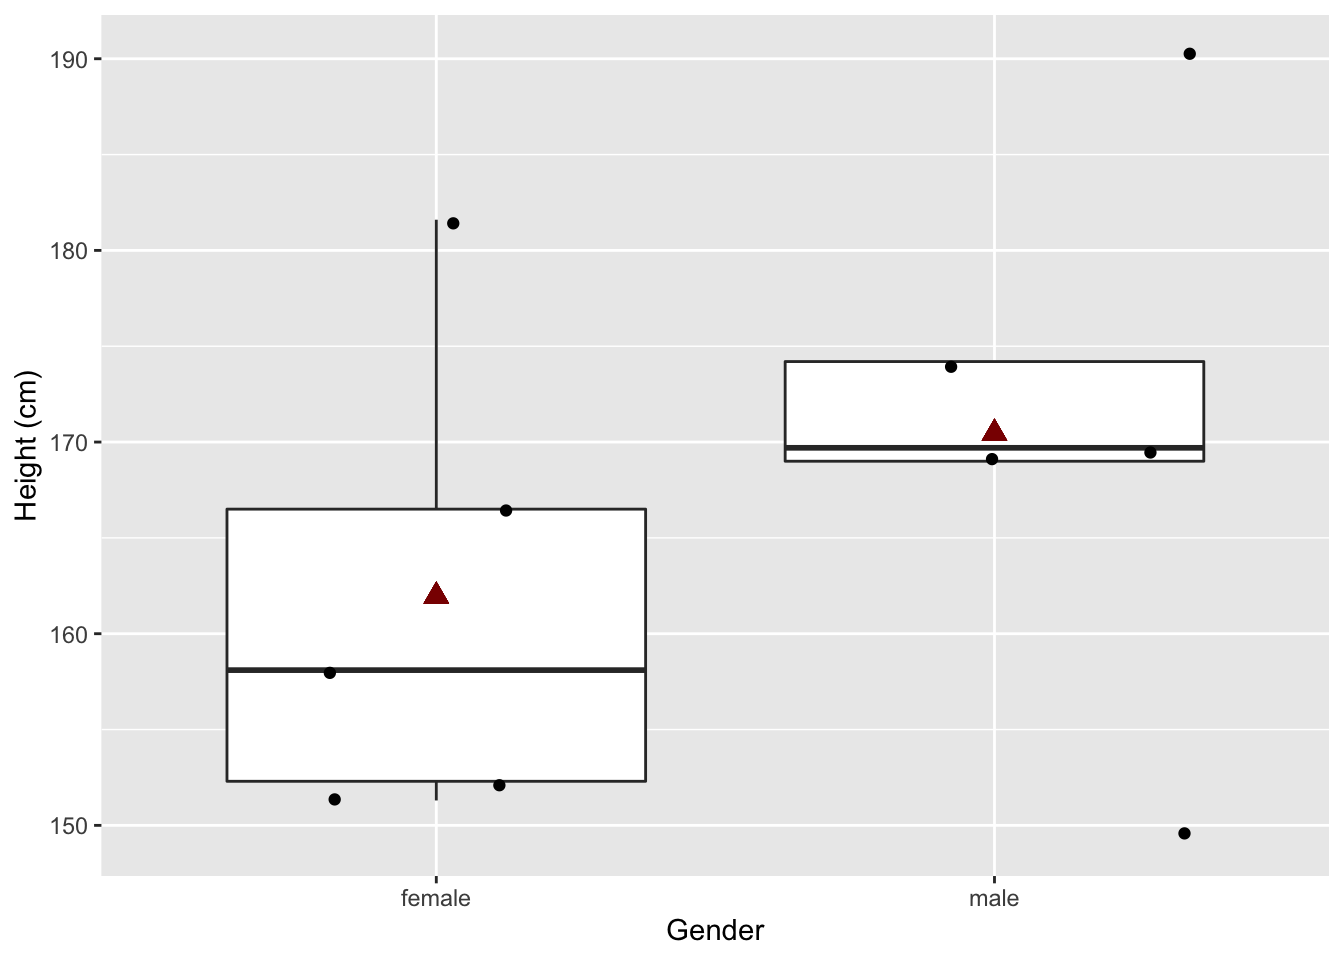
\includegraphics{Statistiek_2020_2021_files/figure-latex/unnamed-chunk-22-1.pdf}

\begin{Shaded}
\begin{Highlighting}[]
\NormalTok{res }\OperatorTok{\%\textgreater{}\%}\StringTok{ }\KeywordTok{ggplot}\NormalTok{(}\KeywordTok{aes}\NormalTok{(}\DataTypeTok{y =}\NormalTok{ verschil)) }\OperatorTok{+}\StringTok{ }\KeywordTok{geom\_boxplot}\NormalTok{() }\OperatorTok{+}\StringTok{ }
\StringTok{    }\KeywordTok{ylab}\NormalTok{(}\StringTok{"Gemiddeld Verschil (cm)"}\NormalTok{)}
\end{Highlighting}
\end{Shaded}

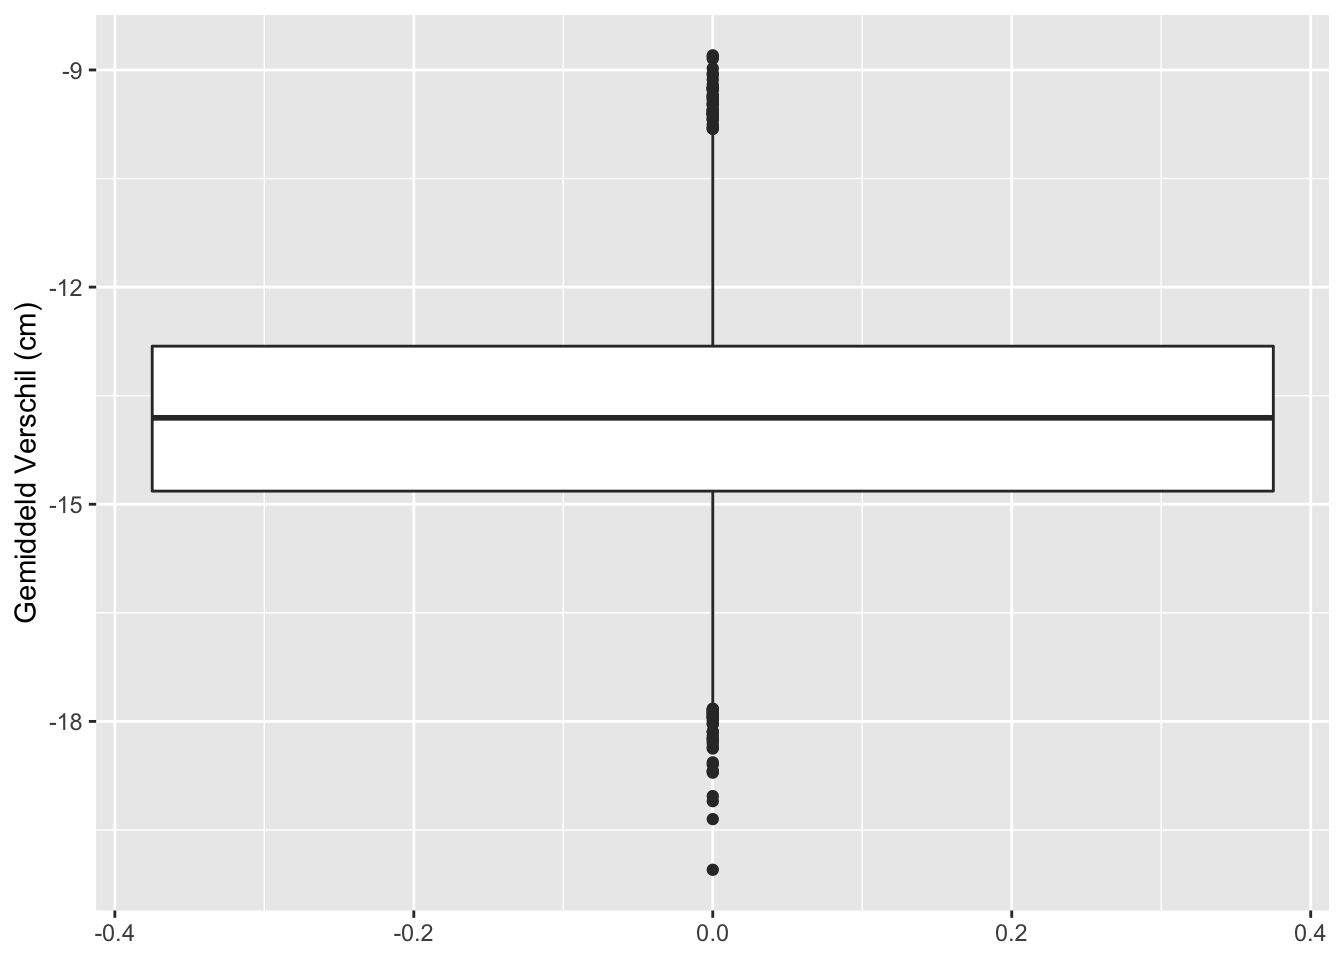
\includegraphics{Statistiek_2020_2021_files/figure-latex/unnamed-chunk-22-2.pdf}

\begin{Shaded}
\begin{Highlighting}[]
\KeywordTok{xlab}\NormalTok{(}\StringTok{""}\NormalTok{)}
\end{Highlighting}
\end{Shaded}

\begin{verbatim}
## $x
## [1] ""
## 
## attr(,"class")
## [1] "labels"
\end{verbatim}

\begin{itemize}
\item
  We zien dus dat we de kans om een verschil te vinden als er in werkelijkheid een verschil is in de populatie kunnen beïnvloeden in de design fase: aan de hand van de steekproefgrootte.
\item
  Hoe meer gegevens hoe makkelijker we het werkelijk verschil oppikken in de steekproef.
\item
  Dat wordt ook geïllustreerd in het gemiddelde verschil in lengte tussen mannen en vrouwen: daar zit in de grote studie veel minder variabiliteit op van steekproef tot steekproef omdat ze veel nauwkeuriger kunnen worden geschat omdat er meer gegevens zijn in de steekproef.
\end{itemize}

\hypertarget{controle-van-vals-positieven}{%
\subsubsection{Controle van vals positieven}\label{controle-van-vals-positieven}}

Wat gebeurt er als er geen verschil is tussen beide groepen?

\begin{itemize}
\item
  We moeten hiervoor experimenten simuleren waarbij de groepen gelijk zijn.
\item
  Hiervoor zullen we twee groepen vergelijken waarvoor de lengte gemiddeld niet verschillend is.
\item
  Dat kunnen we doen door een steekproef te trekken waarbij we voor beide groepen at random subjecten trekken uit de subset van vrouwen in de NHANES studie. Dan weten we dat er on de populatie geen verschil is in lengte tussen beide groepen die we zullen vergelijken.
\item
  Als we toch een verschil vinden in een steekproef dan weten we dat dit een vals positief resultaat is!
\item
  We doen de simulatiestudie opnieuw voor steekproeven met 5 subjecten per groep
\end{itemize}

\begin{Shaded}
\begin{Highlighting}[]
\KeywordTok{set.seed}\NormalTok{(}\DecValTok{13245}\NormalTok{)}
\CommentTok{\# Aantal simulaties en steekproefgrootte per groep}
\NormalTok{nSim \textless{}{-}}\StringTok{ }\DecValTok{10000}
\NormalTok{nSamp \textless{}{-}}\StringTok{ }\DecValTok{5}

\CommentTok{\# We filteren de data vooraf zodat we dit niet}
\CommentTok{\# telkens opnieuw hoeven te doen}
\NormalTok{fem \textless{}{-}}\StringTok{ }\NormalTok{nhanesSub }\OperatorTok{\%\textgreater{}\%}\StringTok{ }\KeywordTok{filter}\NormalTok{(Gender }\OperatorTok{==}\StringTok{ "female"}\NormalTok{)}

\CommentTok{\# Simulatie studie Om snelle functies te kunnen}
\CommentTok{\# gebruiken nemen we eerst nSim steekproeven en}
\CommentTok{\# berekenen we daarna alles.}

\NormalTok{femSamps \textless{}{-}}\StringTok{ }\NormalTok{femSamps2 \textless{}{-}}\StringTok{ }\KeywordTok{matrix}\NormalTok{(}\OtherTok{NA}\NormalTok{, }\DataTypeTok{nrow =}\NormalTok{ nSamp, }\DataTypeTok{ncol =}\NormalTok{ nSim)}
\ControlFlowTok{for}\NormalTok{ (i }\ControlFlowTok{in} \DecValTok{1}\OperatorTok{:}\NormalTok{nSim) \{}
\NormalTok{    femSamps[, i] \textless{}{-}}\StringTok{ }\KeywordTok{sample}\NormalTok{(fem}\OperatorTok{$}\NormalTok{Height, nSamp)}
\NormalTok{    femSamps2[, i] \textless{}{-}}\StringTok{ }\KeywordTok{sample}\NormalTok{(fem}\OperatorTok{$}\NormalTok{Height, nSamp)}
\NormalTok{\}}

\NormalTok{res \textless{}{-}}\StringTok{ }\KeywordTok{data.frame}\NormalTok{(}\DataTypeTok{verschil =} \KeywordTok{colMeans}\NormalTok{(femSamps) }\OperatorTok{{-}}\StringTok{ }\KeywordTok{colMeans}\NormalTok{(femSamps2), }
\NormalTok{    Rfast}\OperatorTok{::}\KeywordTok{ttests}\NormalTok{(femSamps, femSamps2))}

\KeywordTok{sum}\NormalTok{(res}\OperatorTok{$}\NormalTok{pvalue }\OperatorTok{\textless{}}\StringTok{ }\FloatTok{0.05} \OperatorTok{\&}\StringTok{ }\NormalTok{res}\OperatorTok{$}\NormalTok{verschil }\OperatorTok{\textless{}}\StringTok{ }\DecValTok{0}\NormalTok{)}
\end{Highlighting}
\end{Shaded}

\begin{verbatim}
## [1] 213
\end{verbatim}

\begin{Shaded}
\begin{Highlighting}[]
\KeywordTok{sum}\NormalTok{(res}\OperatorTok{$}\NormalTok{pvalue }\OperatorTok{\textgreater{}=}\StringTok{ }\FloatTok{0.05}\NormalTok{)}
\end{Highlighting}
\end{Shaded}

\begin{verbatim}
## [1] 9558
\end{verbatim}

\begin{Shaded}
\begin{Highlighting}[]
\KeywordTok{sum}\NormalTok{(res}\OperatorTok{$}\NormalTok{pvalue }\OperatorTok{\textless{}}\StringTok{ }\FloatTok{0.05} \OperatorTok{\&}\StringTok{ }\NormalTok{res}\OperatorTok{$}\NormalTok{verschil }\OperatorTok{\textgreater{}}\StringTok{ }\DecValTok{0}\NormalTok{)}
\end{Highlighting}
\end{Shaded}

\begin{verbatim}
## [1] 229
\end{verbatim}

\begin{Shaded}
\begin{Highlighting}[]
\NormalTok{res }\OperatorTok{\%\textgreater{}\%}\StringTok{ }\KeywordTok{ggplot}\NormalTok{(}\KeywordTok{aes}\NormalTok{(}\DataTypeTok{x =}\NormalTok{ verschil, }\DataTypeTok{y =} \OperatorTok{{-}}\KeywordTok{log10}\NormalTok{(pvalue), }
    \DataTypeTok{color =}\NormalTok{ pvalue }\OperatorTok{\textless{}}\StringTok{ }\FloatTok{0.05}\NormalTok{)) }\OperatorTok{+}\StringTok{ }\KeywordTok{geom\_point}\NormalTok{() }\OperatorTok{+}\StringTok{ }\KeywordTok{xlab}\NormalTok{(}\StringTok{"Gemiddeld Verschil (cm)"}\NormalTok{) }\OperatorTok{+}\StringTok{ }
\StringTok{    }\KeywordTok{ylab}\NormalTok{(}\StringTok{"Statistische Significantie ({-}log10 p)"}\NormalTok{)}
\end{Highlighting}
\end{Shaded}

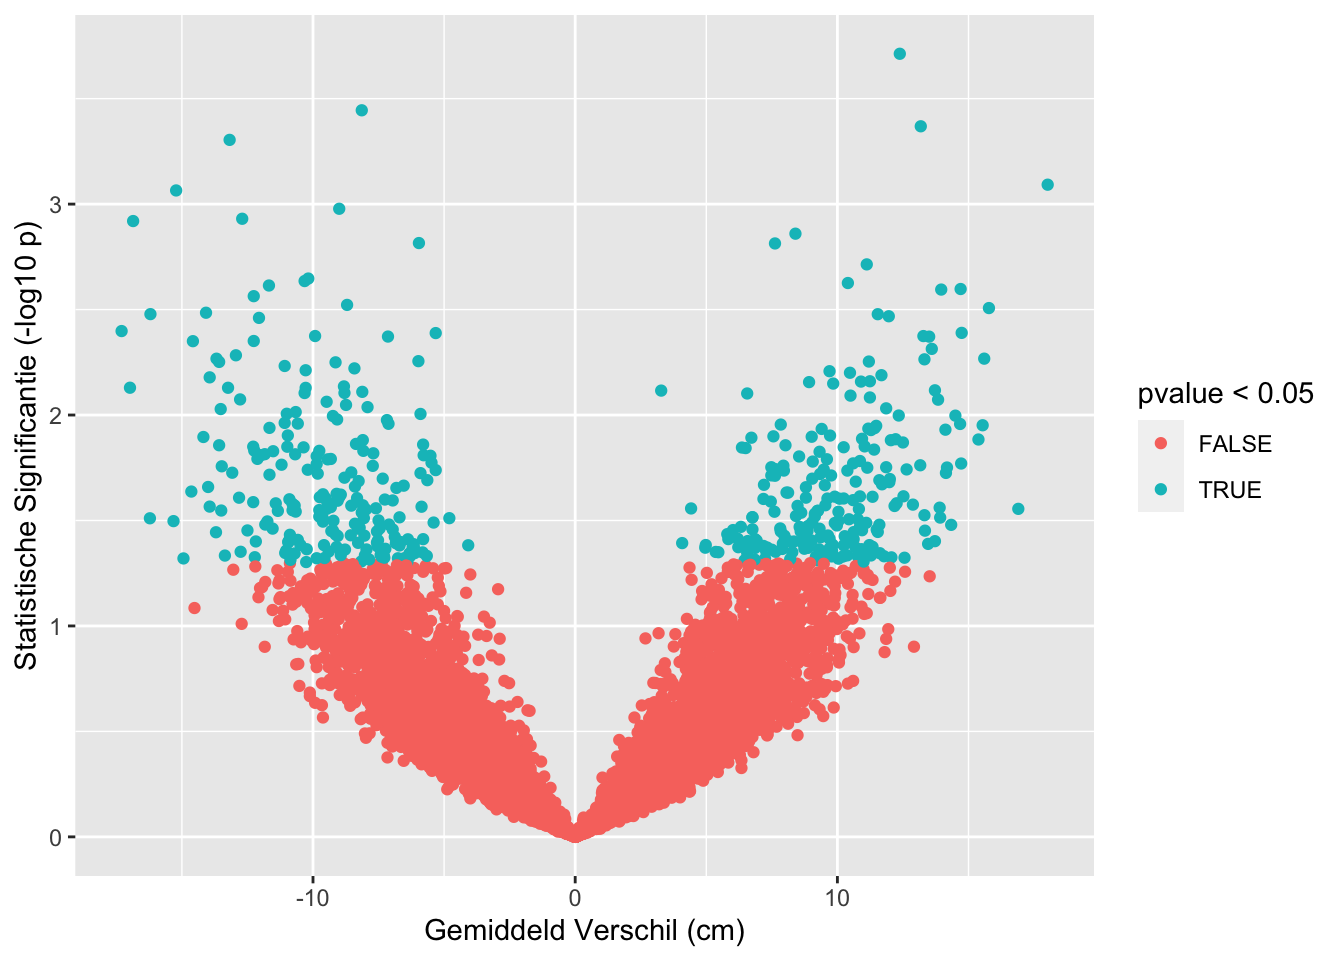
\includegraphics{Statistiek_2020_2021_files/figure-latex/unnamed-chunk-23-1.pdf}

\begin{Shaded}
\begin{Highlighting}[]
\NormalTok{res }\OperatorTok{\%\textgreater{}\%}\StringTok{ }\KeywordTok{ggplot}\NormalTok{(}\KeywordTok{aes}\NormalTok{(}\DataTypeTok{y =}\NormalTok{ verschil)) }\OperatorTok{+}\StringTok{ }\KeywordTok{geom\_boxplot}\NormalTok{() }\OperatorTok{+}\StringTok{ }
\StringTok{    }\KeywordTok{ylab}\NormalTok{(}\StringTok{"Gemiddeld Verschil (cm)"}\NormalTok{)}
\end{Highlighting}
\end{Shaded}

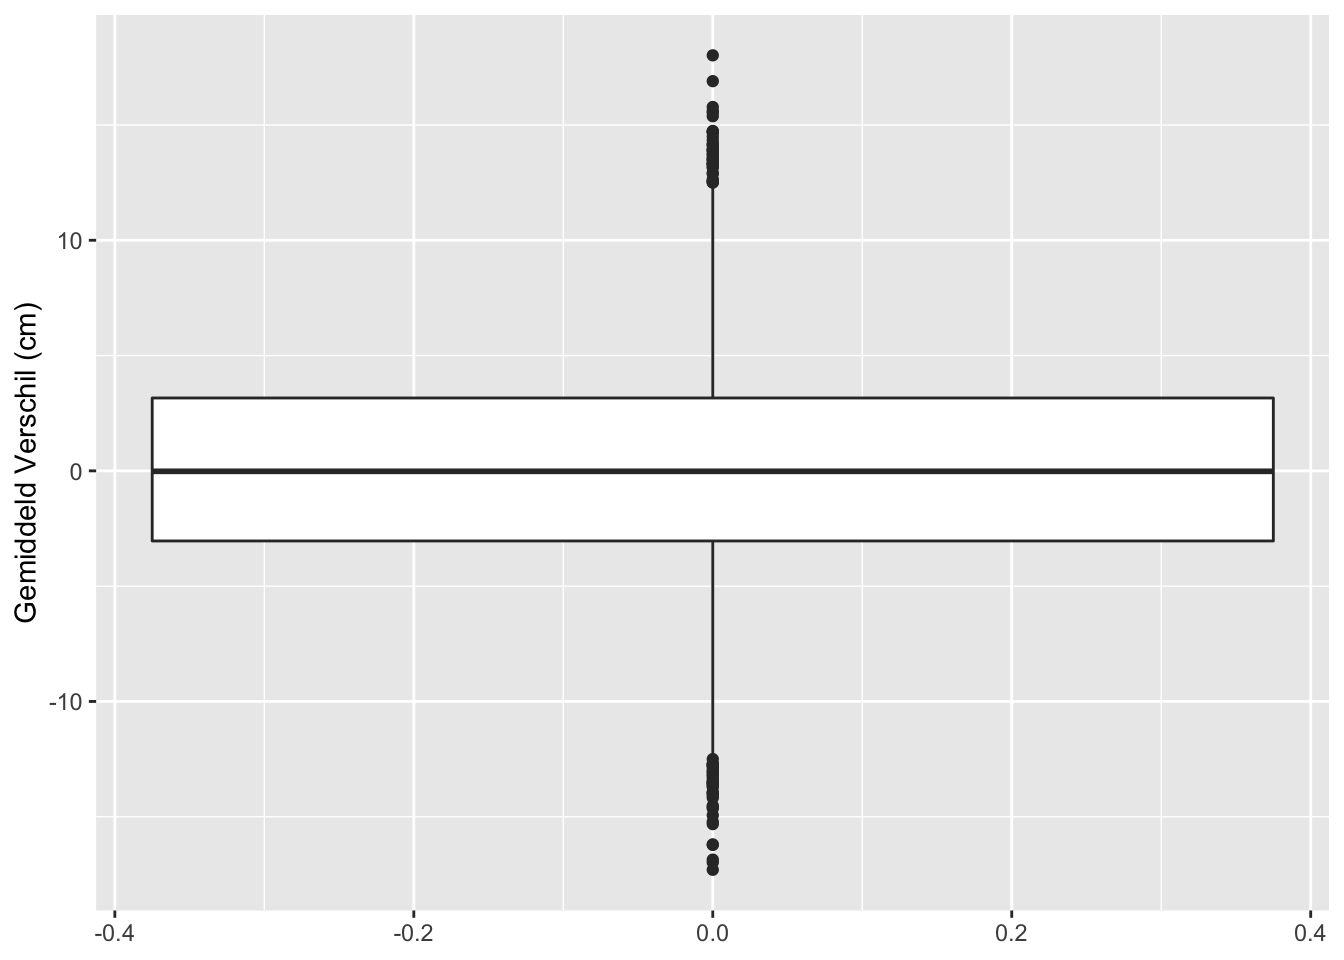
\includegraphics{Statistiek_2020_2021_files/figure-latex/unnamed-chunk-23-2.pdf}

\begin{Shaded}
\begin{Highlighting}[]
\KeywordTok{xlab}\NormalTok{(}\StringTok{""}\NormalTok{)}
\end{Highlighting}
\end{Shaded}

\begin{verbatim}
## $x
## [1] ""
## 
## attr(,"class")
## [1] "labels"
\end{verbatim}

Op basis van 10000 steekproeven zien we dat we in 442 steekproeven ten onrechte besluiten dat er een verschil is in gemiddelde lengte tussen twee groepen vrouwen.

Met de statistische analyse controleren we dus het aantal vals positieve resultaten correct op 5\%.

\emph{Wat gebeurt er als we het aantal observaties verhogen?}

We simuleren opnieuw experimenten met 50 subjecten per groep maar we trekken de subjecten opnieuw telkens uit de populatie van vrouwen.

\begin{Shaded}
\begin{Highlighting}[]
\KeywordTok{set.seed}\NormalTok{(}\DecValTok{1345}\NormalTok{)}
\CommentTok{\# Aantal simulaties en steekproefgrootte per groep}
\NormalTok{nSim \textless{}{-}}\StringTok{ }\DecValTok{10000}
\NormalTok{nSamp \textless{}{-}}\StringTok{ }\DecValTok{50}

\CommentTok{\# We filteren de data vooraf zodat we dit niet}
\CommentTok{\# telkens opnieuw hoeven te doen}
\NormalTok{fem \textless{}{-}}\StringTok{ }\NormalTok{nhanesSub }\OperatorTok{\%\textgreater{}\%}\StringTok{ }\KeywordTok{filter}\NormalTok{(Gender }\OperatorTok{==}\StringTok{ "female"}\NormalTok{)}

\CommentTok{\# Simulatie studie Om snelle functies te kunnen}
\CommentTok{\# gebruiken nemen we eerst nSim steekproeven en}
\CommentTok{\# berekenen we daarna alles.}

\NormalTok{femSamps \textless{}{-}}\StringTok{ }\NormalTok{femSamps2 \textless{}{-}}\StringTok{ }\KeywordTok{matrix}\NormalTok{(}\OtherTok{NA}\NormalTok{, }\DataTypeTok{nrow =}\NormalTok{ nSamp, }\DataTypeTok{ncol =}\NormalTok{ nSim)}
\ControlFlowTok{for}\NormalTok{ (i }\ControlFlowTok{in} \DecValTok{1}\OperatorTok{:}\NormalTok{nSim) \{}
\NormalTok{    femSamps[, i] \textless{}{-}}\StringTok{ }\KeywordTok{sample}\NormalTok{(fem}\OperatorTok{$}\NormalTok{Height, nSamp)}
\NormalTok{    femSamps2[, i] \textless{}{-}}\StringTok{ }\KeywordTok{sample}\NormalTok{(fem}\OperatorTok{$}\NormalTok{Height, nSamp)}
\NormalTok{\}}

\NormalTok{res \textless{}{-}}\StringTok{ }\KeywordTok{data.frame}\NormalTok{(}\DataTypeTok{verschil =} \KeywordTok{colMeans}\NormalTok{(femSamps) }\OperatorTok{{-}}\StringTok{ }\KeywordTok{colMeans}\NormalTok{(femSamps2), }
\NormalTok{    Rfast}\OperatorTok{::}\KeywordTok{ttests}\NormalTok{(femSamps, femSamps2))}

\KeywordTok{sum}\NormalTok{(res}\OperatorTok{$}\NormalTok{pvalue }\OperatorTok{\textless{}}\StringTok{ }\FloatTok{0.05} \OperatorTok{\&}\StringTok{ }\NormalTok{res}\OperatorTok{$}\NormalTok{verschil }\OperatorTok{\textless{}}\StringTok{ }\DecValTok{0}\NormalTok{)}
\end{Highlighting}
\end{Shaded}

\begin{verbatim}
## [1] 271
\end{verbatim}

\begin{Shaded}
\begin{Highlighting}[]
\KeywordTok{sum}\NormalTok{(res}\OperatorTok{$}\NormalTok{pvalue }\OperatorTok{\textgreater{}=}\StringTok{ }\FloatTok{0.05}\NormalTok{)}
\end{Highlighting}
\end{Shaded}

\begin{verbatim}
## [1] 9501
\end{verbatim}

\begin{Shaded}
\begin{Highlighting}[]
\KeywordTok{sum}\NormalTok{(res}\OperatorTok{$}\NormalTok{pvalue }\OperatorTok{\textless{}}\StringTok{ }\FloatTok{0.05} \OperatorTok{\&}\StringTok{ }\NormalTok{res}\OperatorTok{$}\NormalTok{verschil }\OperatorTok{\textgreater{}}\StringTok{ }\DecValTok{0}\NormalTok{)}
\end{Highlighting}
\end{Shaded}

\begin{verbatim}
## [1] 228
\end{verbatim}

\begin{Shaded}
\begin{Highlighting}[]
\NormalTok{res }\OperatorTok{\%\textgreater{}\%}\StringTok{ }\KeywordTok{ggplot}\NormalTok{(}\KeywordTok{aes}\NormalTok{(}\DataTypeTok{x =}\NormalTok{ verschil, }\DataTypeTok{y =} \OperatorTok{{-}}\KeywordTok{log10}\NormalTok{(pvalue), }
    \DataTypeTok{color =}\NormalTok{ pvalue }\OperatorTok{\textless{}}\StringTok{ }\FloatTok{0.05}\NormalTok{)) }\OperatorTok{+}\StringTok{ }\KeywordTok{geom\_point}\NormalTok{() }\OperatorTok{+}\StringTok{ }\KeywordTok{xlab}\NormalTok{(}\StringTok{"Gemiddeld Verschil (cm)"}\NormalTok{) }\OperatorTok{+}\StringTok{ }
\StringTok{    }\KeywordTok{ylab}\NormalTok{(}\StringTok{"Statistische Significantie ({-}log10 p)"}\NormalTok{)}
\end{Highlighting}
\end{Shaded}

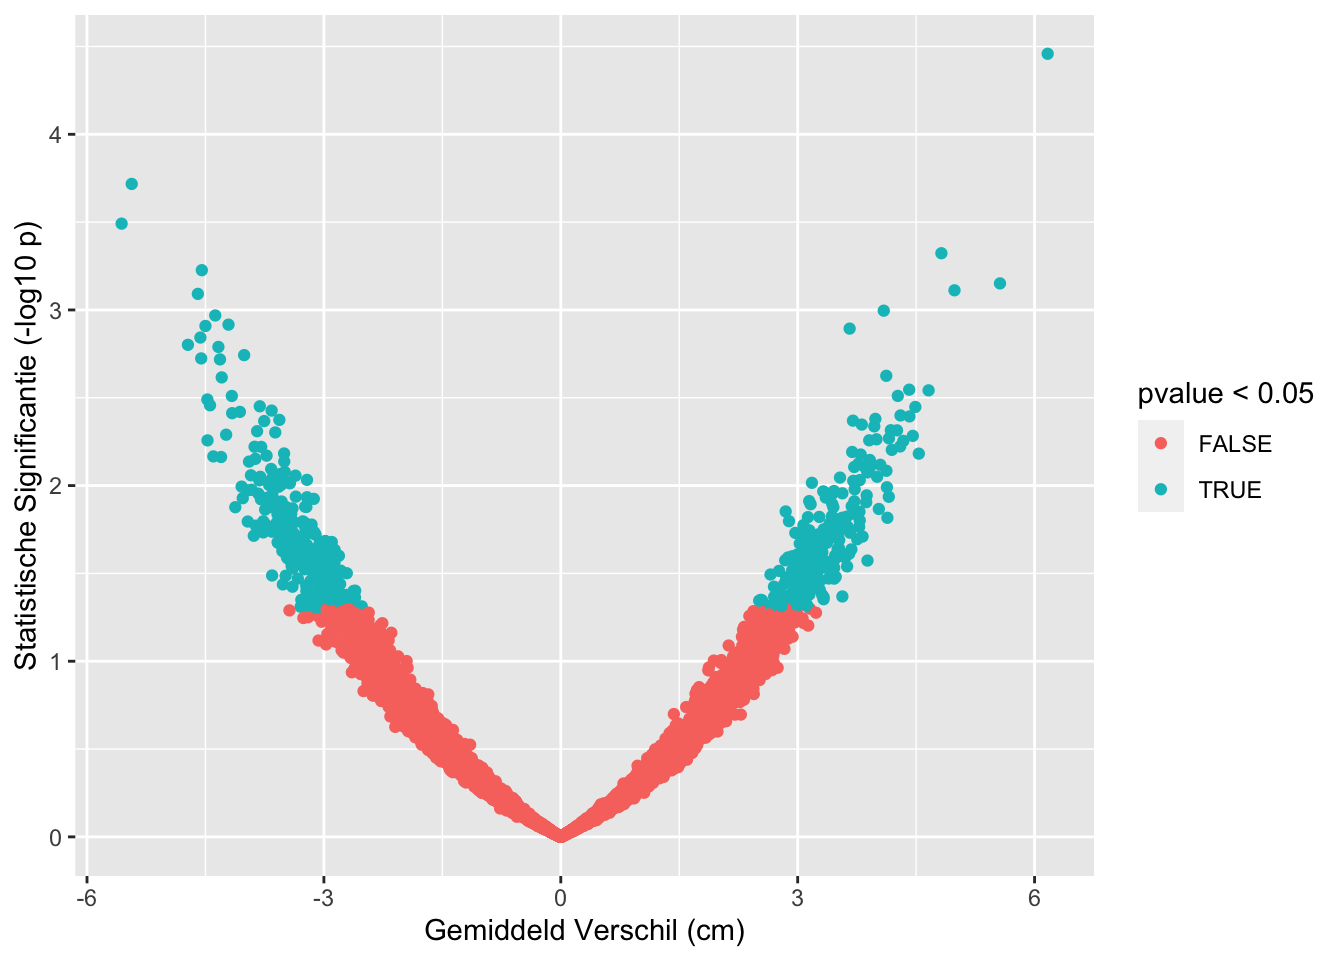
\includegraphics{Statistiek_2020_2021_files/figure-latex/unnamed-chunk-24-1.pdf}

\begin{Shaded}
\begin{Highlighting}[]
\NormalTok{res }\OperatorTok{\%\textgreater{}\%}\StringTok{ }\KeywordTok{ggplot}\NormalTok{(}\KeywordTok{aes}\NormalTok{(}\DataTypeTok{y =}\NormalTok{ verschil)) }\OperatorTok{+}\StringTok{ }\KeywordTok{geom\_boxplot}\NormalTok{() }\OperatorTok{+}\StringTok{ }
\StringTok{    }\KeywordTok{ylab}\NormalTok{(}\StringTok{"Gemiddeld Verschil (cm)"}\NormalTok{)}
\end{Highlighting}
\end{Shaded}

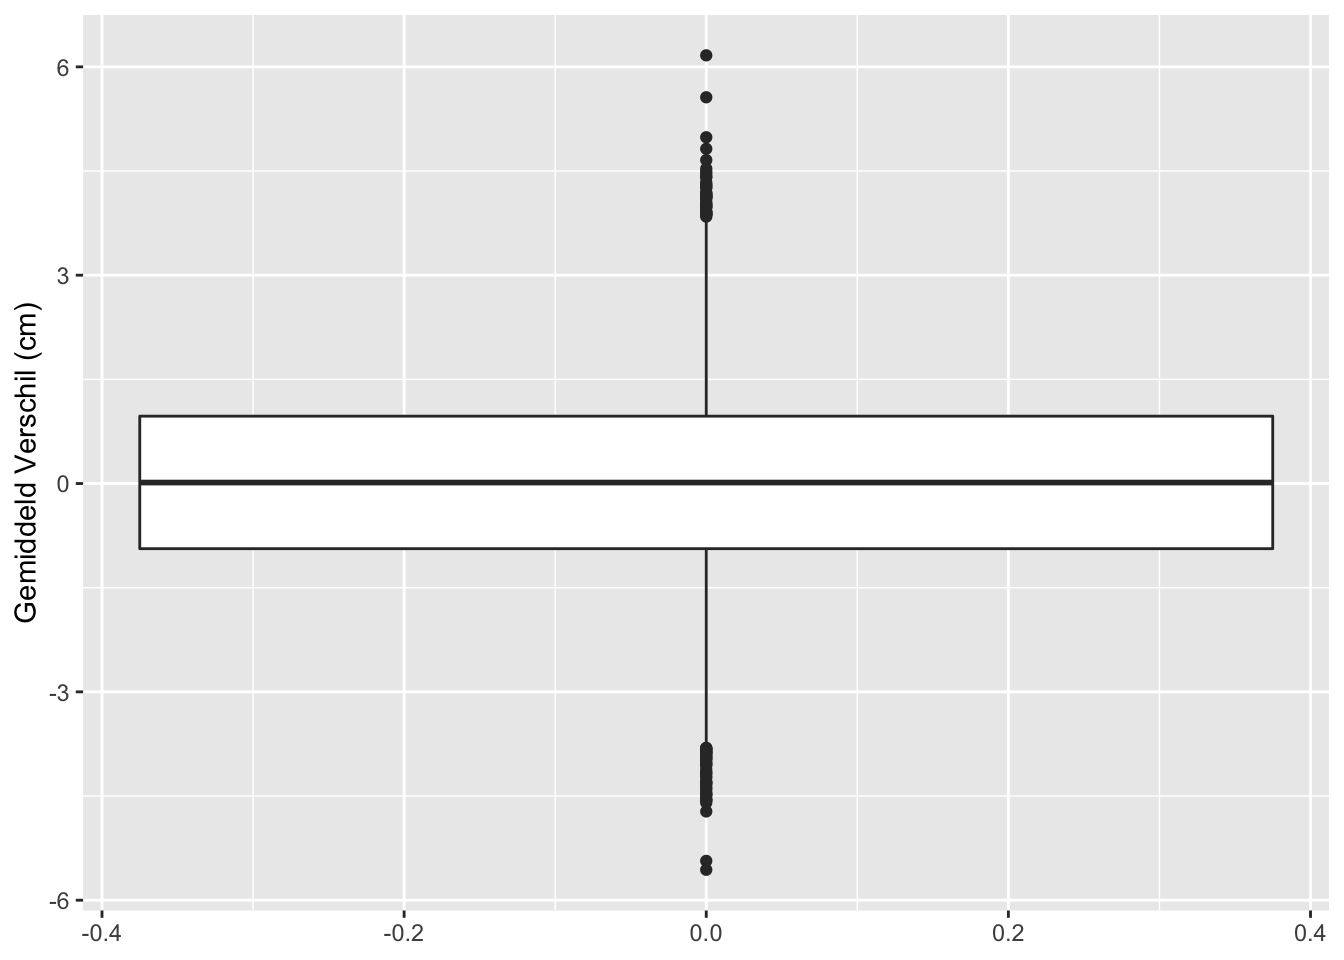
\includegraphics{Statistiek_2020_2021_files/figure-latex/unnamed-chunk-24-2.pdf}

\begin{Shaded}
\begin{Highlighting}[]
\KeywordTok{xlab}\NormalTok{(}\StringTok{""}\NormalTok{)}
\end{Highlighting}
\end{Shaded}

\begin{verbatim}
## $x
## [1] ""
## 
## attr(,"class")
## [1] "labels"
\end{verbatim}

Op basis van 10000 steekproeven zien we dat we in 499 steekproeven ten onrechte besluiten dat er een verschil is in gemiddelde lengte tussen twee groepen vrouwen.

Met de statistische analyse controleren we dus ook bij het nemen van een grote steekproef het aantal vals positieve resultaten correct op 5\%. (Vals positief: Op basis van de steekproef besluiten dat er gemiddeld een verschil is in lengte tussen beide groepen terwijl er in werkelijkheid geen verschil is in de populatie.)

\hypertarget{conclusies}{%
\subsection{Conclusies}\label{conclusies}}

\begin{enumerate}
\def\labelenumi{\arabic{enumi}.}
\item
  In elke steekproef worden at random andere proefpersonen uit de populatie getrokken.
\item
  Hierdoor verschillen lengte metingen van steekproef tot steekproef.
\item
  Dus ook het geschatte gemiddeldes en standaard deviaties.
\item
  Ook onze conclusies zijn onzeker en kunnen wijzigen van steekproef tot steekproef.
\item
  Met statistiek controleren we de kans op het trekken foute conclusies.
\end{enumerate}

\hypertarget{case-study-salk-vaccin}{%
\section{Case study: Salk vaccin}\label{case-study-salk-vaccin}}

In 1916, brak de eerste grote polio epidemie uit in de USA.
Begin de jaren 50 ontwikkelde John Salk een vaccin met belovende resultaten in het lab.
In 1954, heeft de National Foundation for Infantile Paralysis (NFIP) een grote studie opgezet om de effectiviteit van het Salk vaccin na te gaan.

\begin{itemize}
\tightlist
\item
  Veronderstel dat de NFIP in 1954 een groot aantal kinderen zou hebben gevaccineerd, wat zouden ze dan kunnen besluiten als de polio incidentie in 1954 lager was dan in 1953?
\end{itemize}

Neen, het zou gekund hebben dat het verschil in polio incidentie veroorzaakt werd door het feit dat de infectie minder hevig was in 1954.
We hebben dus een controle nodig!

\hypertarget{nfip-study}{%
\subsection{NFIP Study}\label{nfip-study}}

\hypertarget{design}{%
\subsubsection{Design}\label{design}}

\begin{itemize}
\tightlist
\item
  Grote simultane studie met gevaccineerde kinderen (cases) en ongevaccineerde kinderen (controles).
\item
  In scholen van districten met hoge polio incidentie.
\item
  Cases: kinderen van de tweede graad van het lager onderwijs waarvan de ouders toestemden met vaccinatie.
\item
  Controles: kinderen van de eerste en derde graad.
\end{itemize}

\hypertarget{data}{%
\subsubsection{Data}\label{data}}

\begin{Shaded}
\begin{Highlighting}[]
\NormalTok{nfip \textless{}{-}}\StringTok{ }\KeywordTok{tibble}\NormalTok{(}\DataTypeTok{group =} \KeywordTok{c}\NormalTok{(}\StringTok{"cases"}\NormalTok{, }\StringTok{"controls"}\NormalTok{, }\StringTok{"noConcent"}\NormalTok{), }
    \DataTypeTok{grade =} \KeywordTok{c}\NormalTok{(}\StringTok{"g2"}\NormalTok{, }\StringTok{"g1g3"}\NormalTok{, }\StringTok{"g2"}\NormalTok{), }\DataTypeTok{vaccin =} \KeywordTok{c}\NormalTok{(}\StringTok{"yes"}\NormalTok{, }
        \StringTok{"no"}\NormalTok{, }\StringTok{"no"}\NormalTok{), }\DataTypeTok{total =} \KeywordTok{c}\NormalTok{(}\DecValTok{221998}\NormalTok{, }\DecValTok{725173}\NormalTok{, }\DecValTok{123605}\NormalTok{), }
    \DataTypeTok{polio =} \KeywordTok{c}\NormalTok{(}\DecValTok{54}\NormalTok{, }\DecValTok{391}\NormalTok{, }\DecValTok{56}\NormalTok{)) }\OperatorTok{\%\textgreater{}\%}\StringTok{ }\KeywordTok{mutate}\NormalTok{(}\DataTypeTok{noPolio =}\NormalTok{ total }\OperatorTok{{-}}\StringTok{ }
\StringTok{    }\NormalTok{polio)}
\NormalTok{knitr}\OperatorTok{::}\KeywordTok{kable}\NormalTok{(nfip, }\StringTok{"html"}\NormalTok{)}
\end{Highlighting}
\end{Shaded}

group

grade

vaccin

total

polio

noPolio

cases

g2

yes

221998

54

221944

controls

g1g3

no

725173

391

724782

noConcent

g2

no

123605

56

123549

We zien 54 polio besmettingen bij de gevaccineerde kinderen
en 391 bij de controle groep.

\begin{itemize}
\tightlist
\item
  Kunnen we daaruit besluiten trekken?
\end{itemize}

De twee groepen verschillen echter ook in grootte!

We zullen daarom kijken naar polio incidentie per miljoen kinderen.

\begin{enumerate}
\def\labelenumi{\arabic{enumi}.}
\tightlist
\item
  We voegen een extra column toe aan het nfip data object d.m.v. de mutate functie. We berekenen de incidentie per miljoen kinderen (incidencePM) en slaan de gewijzigde dataset op onder dezelfde naam.
\item
  we maken de tabel opnieuw
\end{enumerate}

\begin{Shaded}
\begin{Highlighting}[]
\NormalTok{nfip \textless{}{-}}\StringTok{ }\NormalTok{nfip }\OperatorTok{\%\textgreater{}\%}\StringTok{ }\KeywordTok{mutate}\NormalTok{(}\DataTypeTok{incidencePM =} \KeywordTok{round}\NormalTok{(nfip}\OperatorTok{$}\NormalTok{polio}\OperatorTok{/}\NormalTok{nfip}\OperatorTok{$}\NormalTok{total }\OperatorTok{*}\StringTok{ }
\StringTok{    }\FloatTok{1e+06}\NormalTok{, }\DecValTok{0}\NormalTok{))}
\NormalTok{knitr}\OperatorTok{::}\KeywordTok{kable}\NormalTok{(nfip, }\StringTok{"html"}\NormalTok{)}
\end{Highlighting}
\end{Shaded}

group

grade

vaccin

total

polio

noPolio

incidencePM

cases

g2

yes

221998

54

221944

243

controls

g1g3

no

725173

391

724782

539

noConcent

g2

no

123605

56

123549

453

\begin{itemize}
\item
  We observeren nu dat de incidentie meer dan dubbel zo hoog is in de controle groep als in de vaccinatie groep.
\item
  We observeren echter ook dat de incidentie lager is in de groep van kinderen uit de tweede graad waarvan de ouders geen toestemming gaven voor inenting!?
\item
  Wat betekent dit?
\end{itemize}

\hypertarget{confounding}{%
\subsection{Confounding}\label{confounding}}

\begin{center}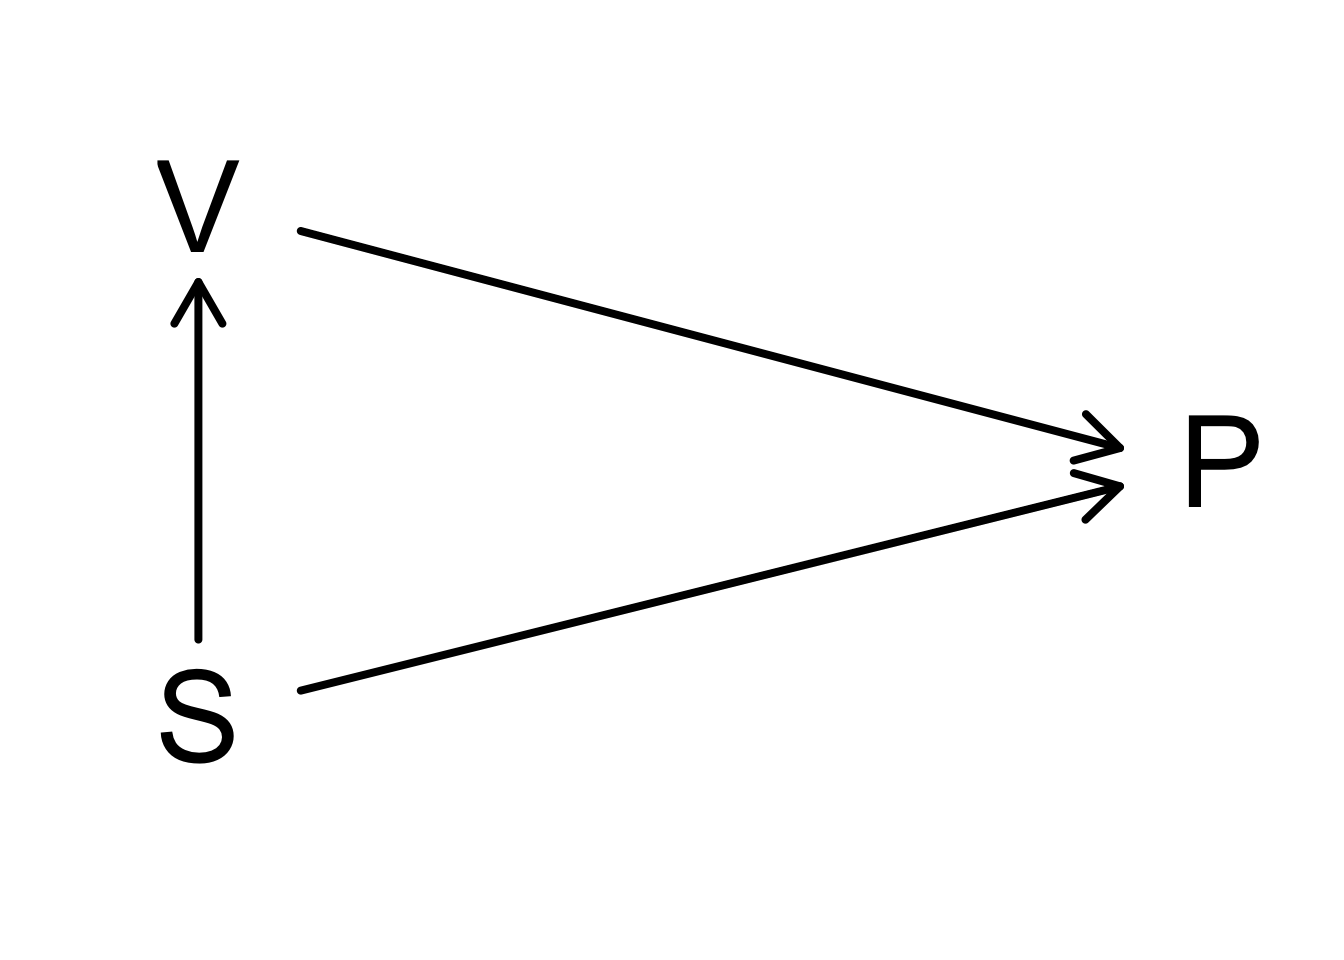
\includegraphics[width=0.5\linewidth]{Statistiek_2020_2021_files/figure-latex/unnamed-chunk-27-1} \end{center}

We observeren een lagere polio (P) incidentie voor kinderen bij wie de ouders geen toestemming gaven dan in de controle groep.
Toestemming voor vaccinatie (V) is geassocieerd met de socio-economische status (S).
Kinderen van lagere socio-economische status zijn meer resistent tegen de ziekte.

Er is dus sprake van confounding: de socio-economische status is geassocieerd met zowel de polio incidentie als met de toestemming op vaccinatie.

Controle groep en gevaccineerde groep zijn dus niet vergelijkbaar:
Ze verschillen in socio economische status en bovendien ook in leeftijd!
We kunnen aan de hand van het experiment het effect van de vaccinatie niet correct inschatten.

\hypertarget{salk-study}{%
\subsection{Salk Study}\label{salk-study}}

\hypertarget{design-1}{%
\subsubsection{Design}\label{design-1}}

Een nieuwe studie werd uitgevoerd: dubbel blinde gerandomiseerde studie.

\begin{itemize}
\tightlist
\item
  Kinderen worden at random toegewezen aan controle of case arm van het experiment nadat de ouders toestemden met vaccinatie.
\item
  Controle: vaccinatie met placebo
\item
  Treatment: vaccinatie met vaccin
\item
  Double blinding:

  \begin{itemize}
  \tightlist
  \item
    ouders en kinderen weten niet of ze werden gevaccineerd of niet
  \item
    medische staf en onderzoekers weten niet of het kind het vaccin of de placebo kreeg
  \end{itemize}
\end{itemize}

\hypertarget{data-1}{%
\subsubsection{Data}\label{data-1}}

\begin{Shaded}
\begin{Highlighting}[]
\NormalTok{salk \textless{}{-}}\StringTok{ }\KeywordTok{data.frame}\NormalTok{(}\DataTypeTok{group =} \KeywordTok{c}\NormalTok{(}\StringTok{"cases"}\NormalTok{, }\StringTok{"control"}\NormalTok{, }\StringTok{"noConcent"}\NormalTok{), }
    \DataTypeTok{treatment =} \KeywordTok{c}\NormalTok{(}\StringTok{"vaccine"}\NormalTok{, }\StringTok{"placebo"}\NormalTok{, }\StringTok{"none"}\NormalTok{), }\DataTypeTok{total =} \KeywordTok{c}\NormalTok{(}\DecValTok{200745}\NormalTok{, }
        \DecValTok{201229}\NormalTok{, }\DecValTok{338778}\NormalTok{), }\DataTypeTok{polio =} \KeywordTok{c}\NormalTok{(}\DecValTok{57}\NormalTok{, }\DecValTok{142}\NormalTok{, }\DecValTok{157}\NormalTok{)) }\OperatorTok{\%\textgreater{}\%}\StringTok{ }
\StringTok{    }\KeywordTok{mutate}\NormalTok{(}\DataTypeTok{noPolio =}\NormalTok{ total }\OperatorTok{{-}}\StringTok{ }\NormalTok{polio, }\DataTypeTok{incidencePM =} \KeywordTok{round}\NormalTok{(polio}\OperatorTok{/}\NormalTok{total }\OperatorTok{*}\StringTok{ }
\StringTok{        }\FloatTok{1e+06}\NormalTok{, }\DecValTok{0}\NormalTok{))}
\NormalTok{knitr}\OperatorTok{::}\KeywordTok{kable}\NormalTok{(salk, }\StringTok{"html"}\NormalTok{)}
\end{Highlighting}
\end{Shaded}

group

treatment

total

polio

noPolio

incidencePM

cases

vaccine

200745

57

200688

284

control

placebo

201229

142

201087

706

noConcent

none

338778

157

338621

463

\begin{itemize}
\item
  We observeren een veel groter effect nu dat cases en controles vergelijkbaar zijn, incidentie van respectievelijk 284 and 706 per miljoen.
\item
  De polio incidentie voor kinderen die geen toestemming geven blijft vergelijkbaar 453 and 463 per miljoen respectievelijk in the NFIP and Salk study.
\end{itemize}

We zullen later in de cursus tonen dat het effect van het vaccin statistisch significant is.

\hypertarget{rol-van-statistiek}{%
\section{Rol van Statistiek}\label{rol-van-statistiek}}

In deze introductie hebben we gezien dat statistiek een belangrijke rol speelt in empirisch onderzoek. We toonden aan dat

\begin{enumerate}
\def\labelenumi{\arabic{enumi}.}
\item
  \emph{Proefopzet} is essentieel

  \begin{itemize}
  \item
    het belangrijk is om de scope van de studie goed te specifiëren voor de start van het experiment
  \item
    randomisatie nodig is om een representatieve steekproef te nemen
  \item
    steekproef grootte is heel belangrijk
  \item
    we moeten ons bewust zijn van Confounding
  \item
    een goede controle is belangrijk
  \end{itemize}
\item
  \emph{Data exploratie en beschrijvende statistiek}:

  \begin{itemize}
  \tightlist
  \item
    exploreren
  \item
    visualiseren
  \item
    samenvatten en beschrijven van geobserveerde data zodat relevante aspecten naar voor komen.
  \end{itemize}
\item
  \emph{Statistische besluitvorming}: aan de hand van statistische modellen bestuderen in hoeverre geobserveerde trends/effecten die geobserveerd worden in een steekproef veralgemeend kunnen worden naar de algemene populatie.
\end{enumerate}

\hypertarget{belangrijke-concepten-conventies}{%
\chapter{Belangrijke concepten \& conventies}\label{belangrijke-concepten-conventies}}

Alle kennisclips die in dit hoofdstuk zijn verwerkt kan je in deze youtube playlist vinden: \href{https://www.youtube.com/playlist?list=PLZH1hP8_LbJJ7apU5sAbRlUsve2nWz5ev}{Kennisclips Hoofdstuk2}

Link naar webpage/script die wordt gebruik in de kennisclips: \href{https://statomics.github.io/sbc20/rmd/02-concepts.html}{script Hoofdstuk2}

\hypertarget{inleiding-1}{%
\section{Inleiding}\label{inleiding-1}}

De verschillende stappen in een studie worden geïllustreerd in
Figuur \ref{fig:pop2Samp2Pop}.
Eerst bepaalt de onderzoeker de \emph{populatie} van interesse.
Gezien het om financiële en logistieke beperkingen vrijwel nooit mogelijk is om de volledige populatie te onderzoeken zal men vervolgens een steekproef nemen uit de populatie.
De manier waarop een steekproef zal worden genomen wordt vastgelegd in het \emph{design van de studie}.
\emph{Proefopzet} of \emph{studie design} is een aparte tak van de statisitiek en is een cruciaal onderdeel van een studie.
Het studie design moet immers garanderen dat de gegevens en resultaten van de steekproef representatief zijn voor de populatie zodat de resultaten van de studie veralgemeneend kunnen worden naar de populatie toe.
Vervolgens wordt de studie uitgevoerd, worden de gegevens verzameld en kan de eigenlijke data-analyse van start gaan.
In een eerste fase is het belangrijk om de gegevens grondig te exploreren.
\emph{Data-exploratie en beschrijvende statistiek} is een tweede tak van de statistiek die toelaat om gegevens van de steekproef te visualiseren, samen te vatten en om inzicht in de data te verwerven.
Dat is belangrijk om de data correct te kunnen modelleren en om aannames na te kunnen gaan die nodig zijn voor de verdere data analyse. Vervolgens zullen we hetgeen we observeren in de steekproef trachten te veralgemenen naar de algemene populatie toe, zodat we algemene conclusies kunnen trekken op populatie-niveau op basis van de steekproef van de studie. Hiervoor zijn methodes nodig van de \emph{statistische besluitvorming}, ook wel \emph{statistische inferentie} genoemd, een derde belangrijke tak van de statistiek.

\begin{figure}

{\centering 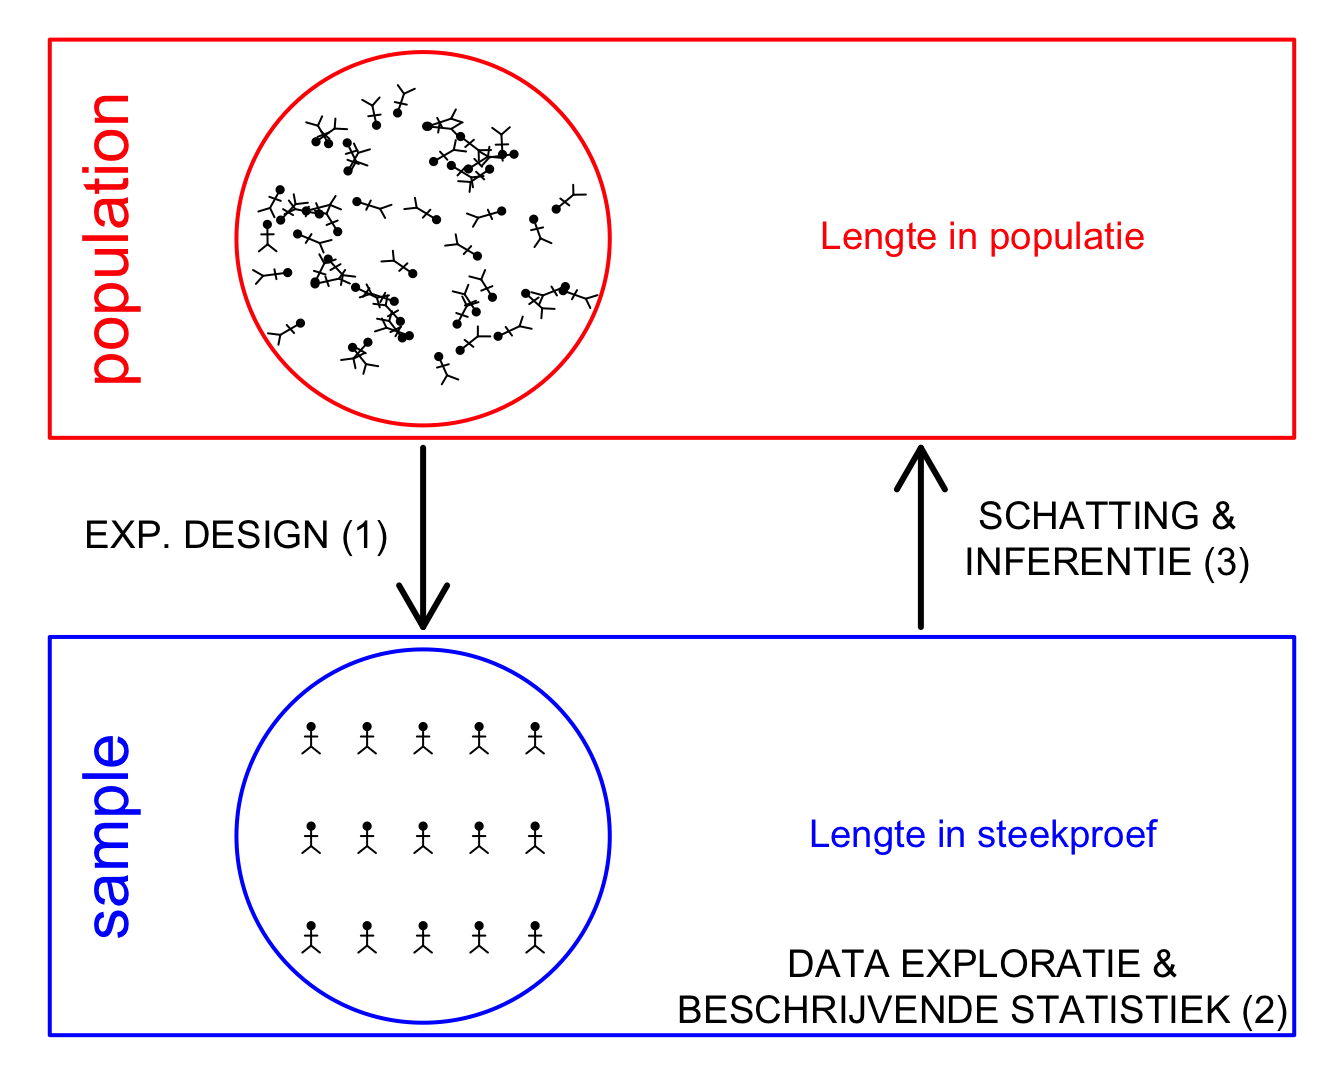
\includegraphics[width=1\linewidth]{Statistiek_2020_2021_files/figure-latex/pop2Samp2Pop-1} 

}

\caption{Verschillende stappen in een studie. (1) In de design fase/ proefopzet definieert de onderzoeker de populatie, bepaalt hij/zij op welke manier een steekproef zal worden genomen uit de populatie en hoe het experiment zal worden uitgevoerd. Ook het volledige data analyse plan moet in deze fase zijn vastgelegd. Vervolgens wordt het experiment uitgevoerd en worden de gegevens verzameld. (2) De gegevens worden vervolgens verkend en samengevat. Hierbij verwerft men inzicht in de gegevens en kunnen aannames worden nagegaan die noodzakelijk zijn voor de verdere data analyse stappen. (3) Tenslotte zal men hetgeen men observeert in de steekproef trachten te veralgemenen naar de populatie toe a.d.h.v. statistische inferentie.}\label{fig:pop2Samp2Pop}
\end{figure}

Vooraleer we dieper ingaan op studie-design, data-exploratie en statistische besluitvorming zullen we eerst enkele concepten introduceren.
We doen dat in dit hoofdstuk aan de hand van de de NHANES studie.

\begin{example}[NHANES studie]
\protect\hypertarget{exm:nhanesExConcepten}{}{\label{exm:nhanesExConcepten} \iffalse (NHANES studie) \fi{} }
\end{example}

De National Health and Nutrition Examination Survey
(NHANES) wordt sinds 1960 op regelmatige basis afgenomen. In dit voorbeeld maken we gebruik van de gegevens die werden verzameld tussen 2009-2012 bij 10000 Amerikanen en die werden opgenomen in het R-pakket NHANES. Er werd een groot aantal fysieke, demografische, nutritionele, levelsstijl en gezondheidskarakteristieken gecollecteerd in deze studie (zie Tabel \ref{tab:nhanesConcepten}).

\textbf{Einde voorbeeld}

\begin{table}

\caption{\label{tab:nhanesConcepten}Overzicht van een aantal variabelen uit de NHANES studie.}
\centering
\begin{tabular}[t]{rlrlrr}
\toprule
ID & Gender & Height & BMI\_WHO & DirectChol & SexNumPartnLife\\
\midrule
51624 & male & 164.7 & 30.0\_plus & 1.29 & 8\\
51625 & male & 105.4 & 12.0\_18.5 & NA & NA\\
51630 & female & 168.4 & 30.0\_plus & 1.16 & 10\\
51638 & male & 133.1 & 12.0\_18.5 & 1.34 & NA\\
51646 & male & 130.6 & 18.5\_to\_24.9 & 1.55 & NA\\
\addlinespace
51647 & female & 166.7 & 25.0\_to\_29.9 & 2.12 & 20\\
\bottomrule
\end{tabular}
\end{table}

\hypertarget{variabelen}{%
\section{Variabelen}\label{variabelen}}

\begin{table}

\caption{\label{tab:nhanesConcepten2}Overzicht van een aantal variabelen uit de NHANES studie.}
\centering
\begin{tabular}[t]{rlrlrr}
\toprule
ID & Gender & Height & BMI\_WHO & DirectChol & SexNumPartnLife\\
\midrule
51624 & male & 164.7 & 30.0\_plus & 1.29 & 8\\
51625 & male & 105.4 & 12.0\_18.5 & NA & NA\\
51630 & female & 168.4 & 30.0\_plus & 1.16 & 10\\
51638 & male & 133.1 & 12.0\_18.5 & 1.34 & NA\\
51646 & male & 130.6 & 18.5\_to\_24.9 & 1.55 & NA\\
\addlinespace
51647 & female & 166.7 & 25.0\_to\_29.9 & 2.12 & 20\\
\bottomrule
\end{tabular}
\end{table}

Een \emph{variabele} is een karakteristiek (bvb. Systolische bloeddruk, leeftijd, geslacht, \ldots)
die varieert van subject tot subject (bvb. van persoon tot persoon, van dier tot dier, \ldots) in de studie.
Er zijn verschillende \emph{types} variabelen.

\emph{Kwalitatieve variabelen} hebben (meestal) beperkt aantal
uitkomstcategorieën die niet numeriek van aard zijn. Deze worden
onderverdeeld in \emph{nominale variabelen} en \emph{ordinale variabelen}
. Nominale gegevens zijn er die men kan benoemen. Ze worden niet gemeten en kennen geen natuurlijke ordening; bijvoorbeeld geslacht, ras,
bloedgroep, kleur van ogen, \ldots{}
Ordinale variabelen kennen wel een ordening; bijvoorbeeld de BMI klasse volgens het WHO, de rokersstatus (nooit gerookt, ooit gerookt maar
gestopt, actueel roker), \ldots{}

Een ander type van variabelen zijn \emph{numerieke variabelen}. Hierbij maakt men het onderscheid tussen \emph{numerieke discrete variabelen} en \emph{numerieke continue variabelen}.
Numerieke discrete variabelen bestaan uit tellingen, b.v. het aantal partners die men had gedurende het leven (geregistreerd in de NHANES studie), het aantal salamanders van de species \textbf{P. jordani} in een bepaald gebied, het aantal reads dat mapt op een bepaald gen in een genexpressiestudie waarbij men gebruik maakt van next-generation sequencing technologie , \ldots{}

Numerieke continue variabelen kunnen (tenminste in theorie) tussen bepaalde grenzen elke mogelijke waarde aannemen. Bijvoorbeeld, leeftijd is continu want het verschil in leeftijd tussen 2 personen kan in principe willekeurig klein zijn (1 uur, 1 minuut, \ldots). Analoog zijn het gewicht, BMI, fluorescentie-metingen in een ELISA experiment, \ldots{} continue metingen.

In de wetenschappen gaat men vaak continue
gegevens dichotomiseren om ze nominaal te maken. Bijvoorbeeld, systolische
bloeddruk wordt omgezet in hypertensie (\(>140\) mmHg) en normotensie (\(\leq 140\)
mmHg). Dit vereenvoudigt de beschrijving van gegevens. Helaas is dit een
slechte praktijk omdat het meestal leidt tot een aanzienlijk verlies aan informatie en
omdat de aldus bekomen resultaten sterk afhankelijk kunnen zijn van de
gekozen drempelwaarde. In de praktijk worden de uitkomsten van continue
variabelen ook vaak afgerond zodat de vermelde waarden in feite discreet
zijn. Om analoge redenen is het vaak wenselijk om ze als continue variabelen
te blijven beschouwen.

In de praktijk wil men vaak numerieke rangen toekennen aan de verschillende
waarden die ordinale variabelen aannemen. Bijvoorbeeld kan men ervoor kiezen
de codes 1, 2 en 3 toe te kennen aan de meetwaarden \emph{nooit gerookt}, \emph{ooit gerookt maar gestopt} en \emph{actueel roker}.
Het is belangrijk om te beseffen dat de keuze van die numerieke waarden vaak geen betekenis heeft.
Het verschil tussen de toegekende codes (3-2=1, 2-1=1, 3-2=1) is niet bruikbaar gezien men bijvoorbeeld niet onderstellen dat de wijziging in rokerstatus identiek is van \emph{nooit gerookt} naar \emph{ooit gerookt maar gestopt} (2-1=1) en van \emph{ooit gerookt maar gestopt} naar \emph{actueel roker} (3-2=1).

\begin{example}[oefening]
\protect\hypertarget{exm:unnamed-chunk-30}{}{\label{exm:unnamed-chunk-30} \iffalse (oefening) \fi{} }
\end{example}
Geef het type aan van de variabelen in Tabel \ref{tab:nhanesConcepten}

\hypertarget{subsec:pop}{%
\section{Populatie}\label{subsec:pop}}

Het doel van een wetenschappelijke studie is nagenoeg altijd om uitspraken te doen over de algemene populatie.
Stel bijvoorbeeld dat men een grenswaarde wil afleiden om patiënten met hypertensie op te sporen.
Hiervoor zal men eerst de systolische bloeddruk moeten bestuderen bij een populatie van gezonde personen.
Een populatie is meestal continu in verandering.
Bovendien is men meestal niet alleen geïnteresseerd in effecten bij huidige subjecten, maar ook in het effect bij toekomstige subjecten.
De populatie kan dus als oneindig groot worden beschouwd en is op een bepaald ogenblik zelfs niet volledig observeerbaar\footnote{B.v. omdat het ook toekomstige subjecten omvat}.
De populatie kan binnen de statistiek dus worden opgevat als een theoretisch concept die alle huidige en toekomstige subjecten omvat waarover men uitspraken wenst te doen.
In de praktijk zal men dus nooit de volledige populatie kunnen bemonsteren en dient men een steekproef te nemen van de populatie.
Om een representatieve groep subjecten te waarborgen, vertrekt een goede onderzoeksopzet vanuit een belangrijke, precies geformuleerde vraagstelling
omtrent een duidelijk omschreven populatie.
Vaak worden hierbij inclusie- en exclusiecriteria geformuleerd.

\emph{Inclusiecriteria} zijn karakteristieken die een subject/experimentele eenheid moet hebben om tot de populatie te behoren, b.v.

\begin{itemize}
\tightlist
\item
  specifieke ziekte: hypertensie
\item
  leeftijdscategorie
\item
  geslacht
\item
  \ldots{}
\end{itemize}

\emph{Exclusiecriteria} zijn karakteristieken die een subject/experimentele eenheid niet mag hebben om tot de populatie te behoren, b.v.

\begin{itemize}
\tightlist
\item
  geneesmiddelen gebruik
\item
  andere ziekten
\item
  zwangerschap
\item
  \ldots{}
\end{itemize}

Op de subjecten zal men meestal een aantal karakteristieken meten, ook wel \emph{variabelen} genoemd (bvb. Systolische bloeddruk, leeftijd, geslacht, \ldots). Typisch zullen deze variabelen variëren van subject tot subject (bvb. van persoon tot persoon, van dier tot dier, \ldots) in de populatie.

\hypertarget{toevalsveranderlijken-of-toevallige-veranderlijken}{%
\section{Toevalsveranderlijken (of toevallige veranderlijken)}\label{toevalsveranderlijken-of-toevallige-veranderlijken}}

De belangrijke vraag, waar we in in de verdere hoofdstukken dieper op in
zullen gaan, is hoe nauwkeurig we uitspraken kunnen doen over de populatie o.b.v. een groep gemeten subjecten in een steekproef.
De spreiding op de gegevens zal daar een cruciale rol in spelen.
Als de gegevens niet variëren tussen subjecten, dan zullen alle steekproeven uit de populatie hetzelfde resultaat opleveren en zullen de bekomen schattingen niet afwijken van de gezochte populatieparameters.
Als daarentegen de gegevens zeer chaotisch zijn, dan zullen verschillende steekproeven mogelijks zeer verschillende resultaten opleveren, die bijgevolg ver kunnen afwijken van de gezochte populatieparameters.

Om het denkwerk te vergemakkelijken, zullen we hoofdletters gebruiken om aan te geven dat
de bestudeerde karakteristiek (vb. een meetresultaat zoals systolische bloeddruk) variabel is in de populatie,
zonder daarbij concreet over de gerealiseerde waarde
voor een bepaald subject na te denken.
Dergelijke meting of variabele \(X\) wordt
algemeen een \emph{toevalsveranderlijke} of \emph{toevallige veranderlijke} genoemd, (a) omdat ze formeel het
resultaat aanduidt van een \emph{toevallige trekking} van een bepaalde
karakteristiek uit de studiepopulatie en (b) omdat ze bovendien \emph{veranderlijk} is,
niet alle subjecten in de steekproef bezitten immers dezelfde waarde
voor die karakteristiek.

Het makkelijkst om over een toevalsveranderlijke \(X\) na te denken is alsof \(X\) het label voorstelt van
een bepaalde populatiekarakteristiek voor een lukraak individu uit de
bestudeerde populatie, vooraleer haar concrete waarde gemeten werd.
Met andere woorden, een toevalsveranderlijke \(X\) kan men opvatten als onbekende veranderlijke die een meting voorstelt die we plannen te verzamelen, maar nog niet hebben verzameld.
Net zoals observaties kunnen we toevallig veranderlijken klasseren als kwalitatief, kwantitatief, discreet, continu, \ldots.

\hypertarget{beschrijven-van-de-populatie}{%
\section{Beschrijven van de populatie}\label{beschrijven-van-de-populatie}}

Voor we een random variabele meten, kunnen we onmogelijk zeggen hoe hoog de meting precies zal zijn.
De gerealiseerde waarde van \(X\) is dus onderhevig aan random variabiliteit.
De geobserveerde steekproef in de NHANES studie \(x_1, x_2, . . . , x_{10000}\) kan dus als n = 10000 realisaties worden beschouwd van dezelfde random variable X, voor subject \(i\), met \(i = 1,2,...,10000\).
Een random veranderlijke, een karakteristiek van de populatie, wordt beschreven door gebruik te maken van een \emph{verdeling}.

De verdeling beschrijft de waarschijnlijkheid om een bepaalde waarde te observeren voor de toevallig veranderlijke wanneer men volledige lukraak een proefpersoon kiest uit de populatie.

Als we weten hoe de variabele verdeeld is dan kunnen we probabiliteitstheorie gebruiken om de kans te berekenen dat een bepaald voorval (event) zich voordoet: vb wat is de kans dat het IQ van een random subject uit de populatie kleiner of gelijk is aan 80.

\begin{itemize}
\item
  Notatie:

  \begin{itemize}
  \tightlist
  \item
    Event: \(X \leq 80\)
  \item
    Probabiliteit op event: \(Pr(X \leq 80)\)
  \end{itemize}
\end{itemize}

\hypertarget{intermezzo-probabiliteitstheorie}{%
\subsection{Intermezzo probabiliteitstheorie}\label{intermezzo-probabiliteitstheorie}}

\hypertarget{discrete-toevallig-veranderlijken}{%
\subsubsection{Discrete toevallig veranderlijken}\label{discrete-toevallig-veranderlijken}}

Stel dat we een discrete random variabele meten \(X\). Alle mogelijke waarden voor \(X\) worden de steekproefruimte \(\Omega\) genoemd.

\begin{itemize}
\item
  Voor Gender is de steekproefruimte \(\Omega=(0,1)\) met 0 (vrouw) or 1 (man).
\item
  Voor het werpen van een dobbelsteen is de steekproefruimte \(\Omega=(1,2,3,4,5,6)\).
\end{itemize}

Een event \(A\) is een subset van de steekproefruimte

\begin{itemize}
\tightlist
\item
  Een even getal werpen met een dobbelsteen: \(A=(2,4,6)\).
\item
  Kan ook een specifieke waarde zijn \(A=(1)\).
\end{itemize}

Event ruimte \(\mathcal{A}\) is de klasse van alle mogelijke events die kunnen optreden bij een bepaald experiment.

Twee events (\(A_1\) en \(A_2\)) zijn multueel exclusief als ze niet samen op kunnen treden.

\begin{itemize}
\tightlist
\item
  v.b. event van de oneven getallen \(A_1=(1,3,5)\) en het event om \(A_2=(6)\) te gooien.
\item
  Dus \(A_1 \bigcap A_2=\emptyset\).
\end{itemize}

Probabiliteit \(Pr(A)\) is een function \(Pr: A \rightarrow [0,1]\) die voldoet aan

\begin{enumerate}
\def\labelenumi{\arabic{enumi}.}
\tightlist
\item
  \(Pr(A) \geq 0\) en \(Pr(A) \leq 1\) voor elke \(A \in \mathcal{A}\)
\item
  \(Pr(\Omega)=1\)
\item
  Voor multueel exclusieve events \(A_1, A_2, \ldots A_k\) geldt dat \(Pr(A_1 \cup A_2 \ldots \cup A_k)= Pr(A_1) + \ldots + Pr(A_k)\)
\end{enumerate}

Dobbelsteen voorbeeld

\begin{itemize}
\tightlist
\item
  oneven number \(A=(1,3,5)\): is de unie van 3 multueel exclusieve events \(A_1=1\), \(A_2=3\) en \(A_3=5\) zodat
  \(Pr(A)=Pr(1)+Pr(3)+Pr(5)=1/6+1/6+1/6=0.5\)
\item
  \(\Omega=(1,2,3,4,5,6)\): \(Pr(\Omega)=1\)
\end{itemize}

Als we twee subjecten (j en k) onafhankelijk trekken van de populatie dan is de gezamelijke probabiliteit
\(P(X_j,X_k)= P(X_j)P(X_j)\)

\hypertarget{distributie-of-verdeling}{%
\paragraph{Distributie of verdeling}\label{distributie-of-verdeling}}

De distributie of de verdeling van een discrete toevallig veranderlijke \(X\) beschrijft de kans op elke mogelijke waarde van de steekproefruimte.

Voorbeeld: Gender is een binaire variabele (0: vrouw, 1: man) en binaire variabelen volgen een Bernoulli verdeling. 50.8\% van de subjecten in de Amerikaanse populatie zijn vrouw en 49.2\% is man.

Laat \(\pi\) de probabiliteit zijn op een man \(\pi=0.492\).
\[ X\sim \left \{
    \begin{array}{lcl}
    P(X=0) &=& 1-\pi\\
    P(X=1) &=& \pi
    \end{array} \right . \]

\begin{Shaded}
\begin{Highlighting}[]
\KeywordTok{tibble}\NormalTok{(}\DataTypeTok{X =} \KeywordTok{c}\NormalTok{(}\DecValTok{0}\NormalTok{, }\DecValTok{1}\NormalTok{), }\DataTypeTok{prob =} \KeywordTok{c}\NormalTok{(}\FloatTok{0.508}\NormalTok{, }\FloatTok{0.492}\NormalTok{)) }\OperatorTok{\%\textgreater{}\%}\StringTok{ }\KeywordTok{ggplot}\NormalTok{(}\KeywordTok{aes}\NormalTok{(}\DataTypeTok{x =}\NormalTok{ X, }
    \DataTypeTok{xend =}\NormalTok{ X, }\DataTypeTok{y =} \DecValTok{0}\NormalTok{, }\DataTypeTok{yend =}\NormalTok{ prob)) }\OperatorTok{+}\StringTok{ }\KeywordTok{geom\_segment}\NormalTok{() }\OperatorTok{+}\StringTok{ }
\StringTok{    }\KeywordTok{ylab}\NormalTok{(}\StringTok{"Probability"}\NormalTok{)}
\end{Highlighting}
\end{Shaded}

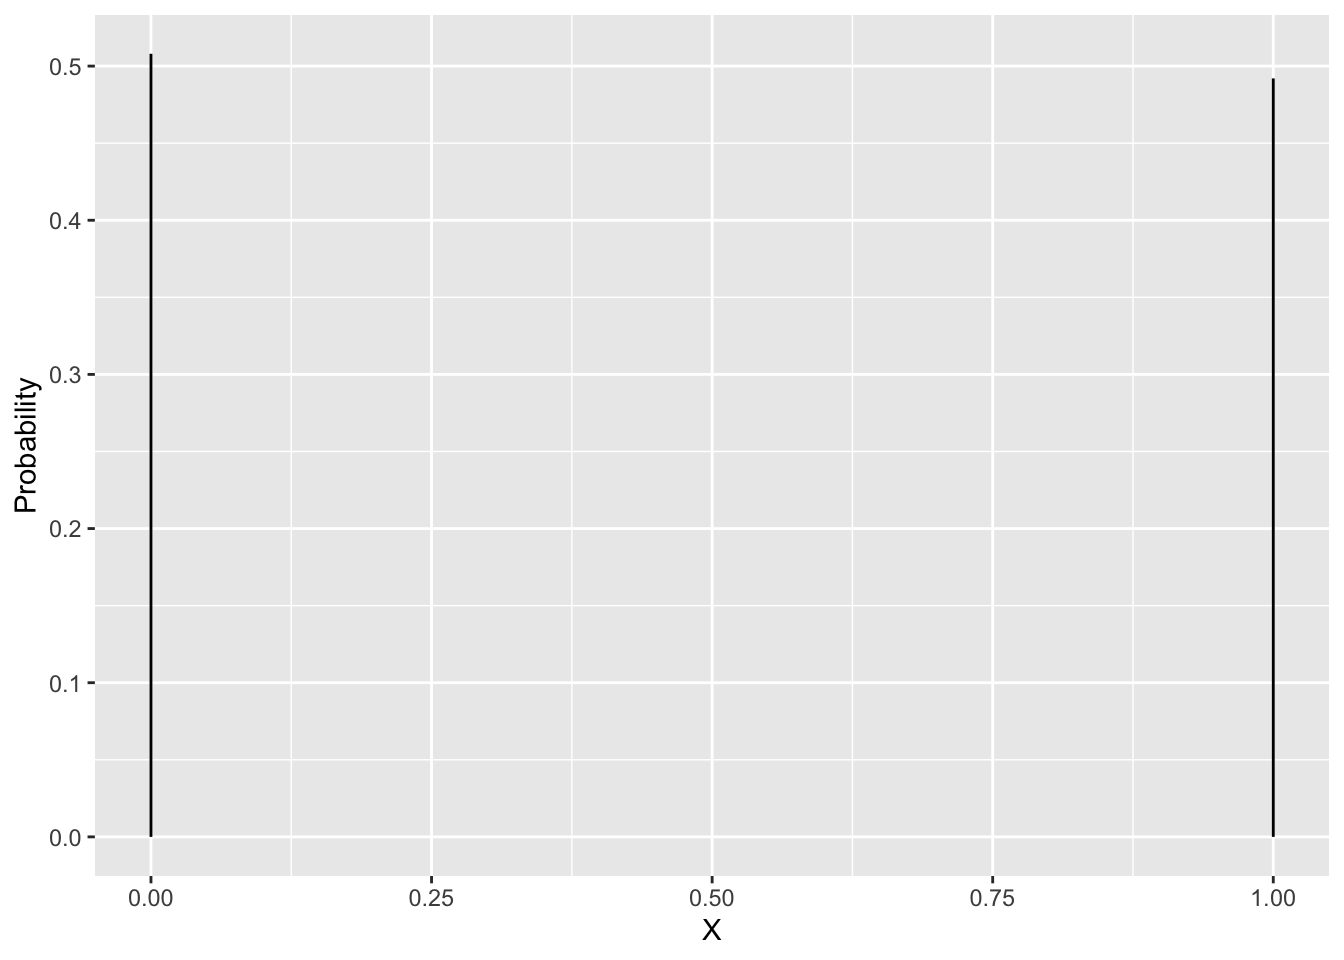
\includegraphics{Statistiek_2020_2021_files/figure-latex/unnamed-chunk-31-1.pdf}

Toevallig veranderlijke \(X\) volgt een Bernoulli verdeling \(B(\pi)\) met parameter \(\pi=0.492\),
\[B(\pi)= \pi^x(1-\pi)^{(1-x)}\]

\hypertarget{cumulative-distributie-functie}{%
\paragraph{Cumulative distributie functie}\label{cumulative-distributie-functie}}

De cumulative distributie functie F(x) geeft de probabiliteit weer om een random variable X te observeren waarvoor geldt dat \(X\leq x\):
\[ F(x) = \sum\limits_{\forall X\leq x} P(x)\]

Gender voorbeeld \(F(0)=1-\pi\) and \(F(1)= P(X=0) + P(X=1)=1\)

\begin{Shaded}
\begin{Highlighting}[]
\KeywordTok{tibble}\NormalTok{(}\DataTypeTok{X =} \KeywordTok{c}\NormalTok{(}\DecValTok{0}\NormalTok{, }\DecValTok{1}\NormalTok{), }\DataTypeTok{cumprob =} \KeywordTok{c}\NormalTok{(}\FloatTok{0.508}\NormalTok{, }\DecValTok{1}\NormalTok{)) }\OperatorTok{\%\textgreater{}\%}\StringTok{ }\KeywordTok{ggplot}\NormalTok{(}\KeywordTok{aes}\NormalTok{(}\DataTypeTok{x =}\NormalTok{ X, }
    \DataTypeTok{xend =}\NormalTok{ X, }\DataTypeTok{y =} \DecValTok{0}\NormalTok{, }\DataTypeTok{yend =}\NormalTok{ cumprob)) }\OperatorTok{+}\StringTok{ }\KeywordTok{geom\_segment}\NormalTok{() }\OperatorTok{+}\StringTok{ }
\StringTok{    }\KeywordTok{ylab}\NormalTok{(}\StringTok{"F(x)"}\NormalTok{)}
\end{Highlighting}
\end{Shaded}

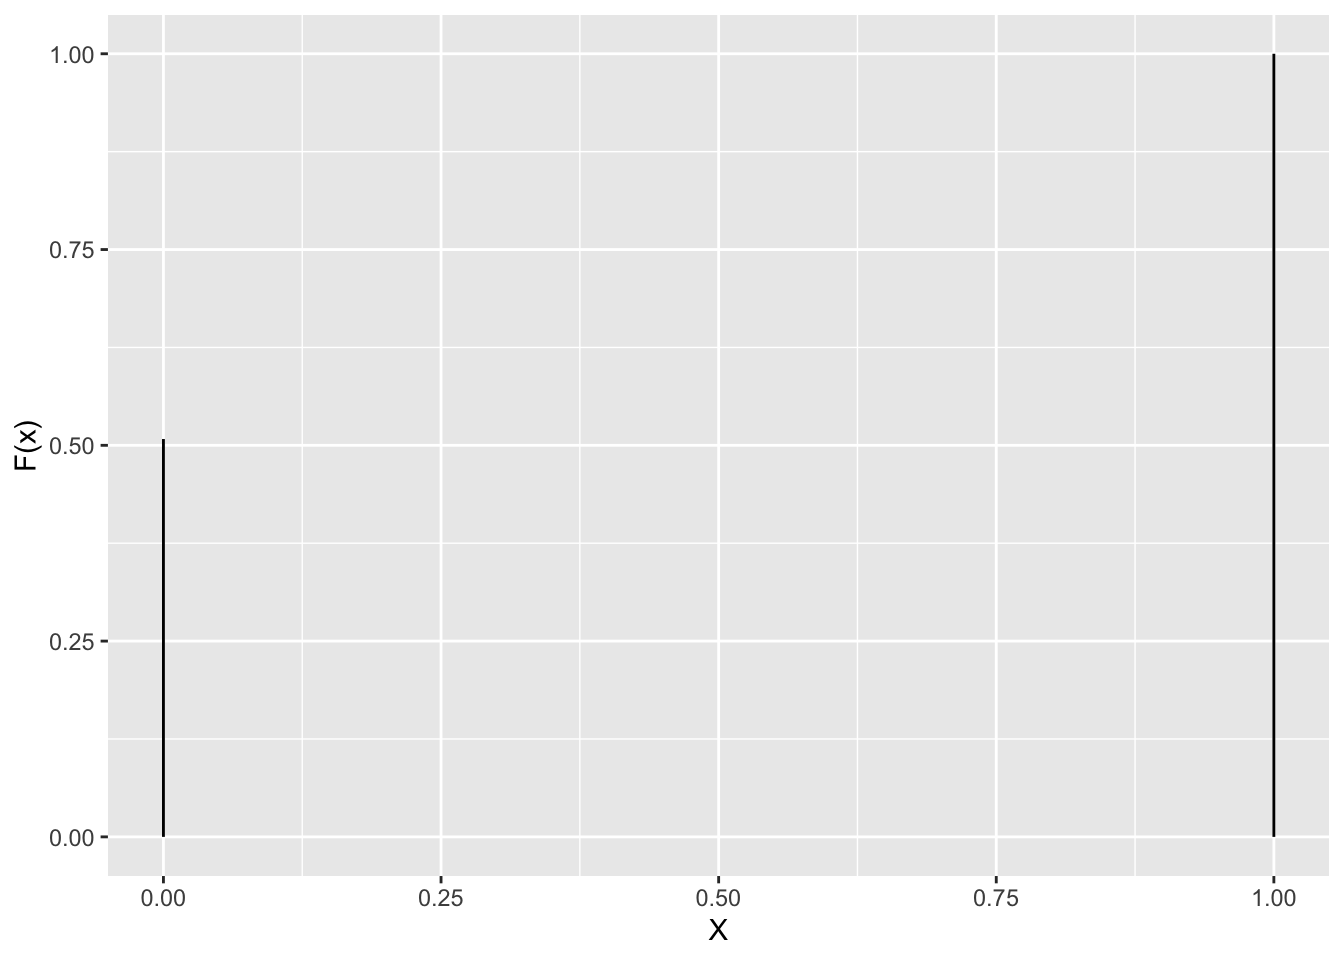
\includegraphics{Statistiek_2020_2021_files/figure-latex/unnamed-chunk-32-1.pdf}

Dobbelsteen voorbeeld:

\begin{Shaded}
\begin{Highlighting}[]
\KeywordTok{tibble}\NormalTok{(}\DataTypeTok{X =} \DecValTok{1}\OperatorTok{:}\DecValTok{6}\NormalTok{, }\DataTypeTok{cumprob =} \KeywordTok{cumsum}\NormalTok{(}\KeywordTok{rep}\NormalTok{(}\DecValTok{1}\OperatorTok{/}\DecValTok{6}\NormalTok{, }\DecValTok{6}\NormalTok{))) }\OperatorTok{\%\textgreater{}\%}\StringTok{ }
\StringTok{    }\KeywordTok{ggplot}\NormalTok{(}\KeywordTok{aes}\NormalTok{(}\DataTypeTok{x =}\NormalTok{ X, }\DataTypeTok{xend =}\NormalTok{ X, }\DataTypeTok{y =} \KeywordTok{rep}\NormalTok{(}\DecValTok{0}\NormalTok{, }\DecValTok{6}\NormalTok{), }\DataTypeTok{yend =}\NormalTok{ cumprob)) }\OperatorTok{+}\StringTok{ }
\StringTok{    }\KeywordTok{geom\_segment}\NormalTok{() }\OperatorTok{+}\StringTok{ }\KeywordTok{ylab}\NormalTok{(}\StringTok{"F(x)"}\NormalTok{)}
\end{Highlighting}
\end{Shaded}

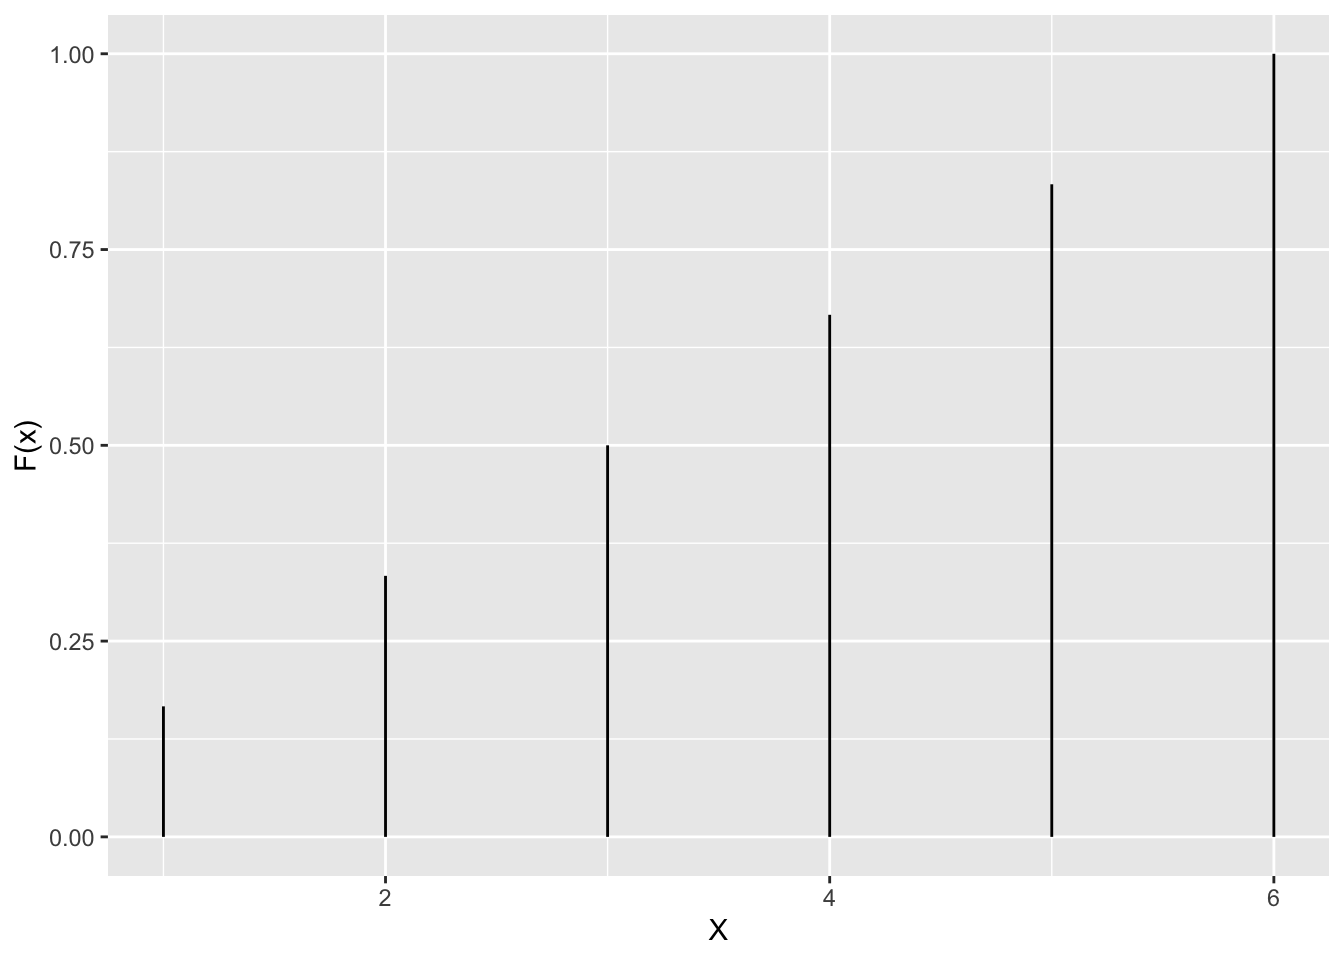
\includegraphics{Statistiek_2020_2021_files/figure-latex/unnamed-chunk-33-1.pdf}

\hypertarget{gemiddelde}{%
\paragraph{Gemiddelde}\label{gemiddelde}}

Het gemiddelde of de verwachte waarde \(E[X]\) van een discrete toevallig veranderlijke \(X\) is gegeven door:

\[E[X]=\sum\limits_{x\in\Omega} x P(X=x)\]

Merk op dat de operator \[E[.]\] staat voor de verwachte waarde van een toevallige veranderlijke of een functie van toevallig veranderlijken.

Gender voorbeeld

\[E[X]= 0 \times (1-\pi) + 1 \times (\pi) = \pi\]

Het gemiddelde is \(E[X]=0.492\).

Dobbelsteen voorbeeld

\(E[X]= 1 \times \frac{1}{6} + 2 \times \frac{1}{6} + \ldots + 6 \times \frac{1}{6} =\) 3.5

\hypertarget{variantie}{%
\paragraph{Variantie}\label{variantie}}

De variantie is een maat voor de variabiliteit van een toevallig veranderlijke en wordt gegeven door:

\[E[(X-E[X])^2]=\sum\limits_{x\in\Omega} (x-E[X])^2 P(X=x)\]

Het is dus de verwachte waarde van de kwadratische afwijkingen van een toevallig veranderlijke rond zijn gemiddelde en is dus een maat voor de variabiliteit of spreiding van de toevallige veranderlijke.

Gender voorbeeld
\begin{eqnarray}
    E[(X-E[X])^2]&=&(0-\pi)^2\times (1-\pi)+(1-\pi)^2 \times \pi\\
    &=& \pi^2 (1-\pi) + (1-\pi)^2 \pi\\
    &=&\pi (1-\pi)(\pi+1-\pi)\\
    &=&\pi(1-\pi)
    \end{eqnarray}

\hypertarget{continue-toevallig-veranderlijke}{%
\subsubsection{Continue toevallig veranderlijke}\label{continue-toevallig-veranderlijke}}

Een continue toevallig veranderlijke kan binnen bepaalde grenzen alle mogelijke waarden aannemen. De kans dat een continue toevallige veranderlijke exact één bepaalde waarde aan te nemen is daarom gelijk aan 0.

De distributie (verdeling) wordt daarom weergegeven a.d.h.v. de densiteitsfunctie of de dichtheidsfunctie \(f(x)\)

Veel biologische karakteristieken zijn approximatief normaal verdeeld (lengte, bloeddruk, IQ, concentratie metingen na logaritmische transformatie)

\[f(x) = \frac{1}{\sqrt{2\pi\sigma^2}} e^{-\frac{(x-\mu)^2}{2\sigma^2}}\]

Dat wordt kort genoteerd als

\[f(x) = N(\mu,\sigma^2)\]

Van het IQ is geweten dat het normale verdeling volgt met gemiddelde \(\mu=100\) en standaardafwijking \(\sigma=15\).

\[IQ \sim N(100,15^2)\]

In R kunnen we de dnorm functie gebruiken om de densiteit te berekenen voor een bepaalde waarde X=x.

\begin{itemize}
\tightlist
\item
  De argumenten van \texttt{dnorm} zijn \texttt{mean} (\(\mu\)) en \texttt{sd} (standaardafwijking \(\sigma\)).
\end{itemize}

\begin{Shaded}
\begin{Highlighting}[]
\NormalTok{iq \textless{}{-}}\StringTok{ }\KeywordTok{tibble}\NormalTok{(}\DataTypeTok{IQ =} \KeywordTok{seq}\NormalTok{(}\DecValTok{40}\NormalTok{, }\DecValTok{150}\NormalTok{, }\FloatTok{0.1}\NormalTok{), }\DataTypeTok{Densiteit =} \KeywordTok{dnorm}\NormalTok{(}\KeywordTok{seq}\NormalTok{(}\DecValTok{40}\NormalTok{, }
    \DecValTok{150}\NormalTok{, }\FloatTok{0.1}\NormalTok{), }\DataTypeTok{mean =} \DecValTok{100}\NormalTok{, }\DataTypeTok{sd =} \DecValTok{15}\NormalTok{))}
\NormalTok{iq }\OperatorTok{\%\textgreater{}\%}\StringTok{ }\KeywordTok{ggplot}\NormalTok{(}\KeywordTok{aes}\NormalTok{(}\DataTypeTok{x =}\NormalTok{ IQ, }\DataTypeTok{y =}\NormalTok{ Densiteit)) }\OperatorTok{+}\StringTok{ }\KeywordTok{geom\_line}\NormalTok{()}
\end{Highlighting}
\end{Shaded}

\begin{center}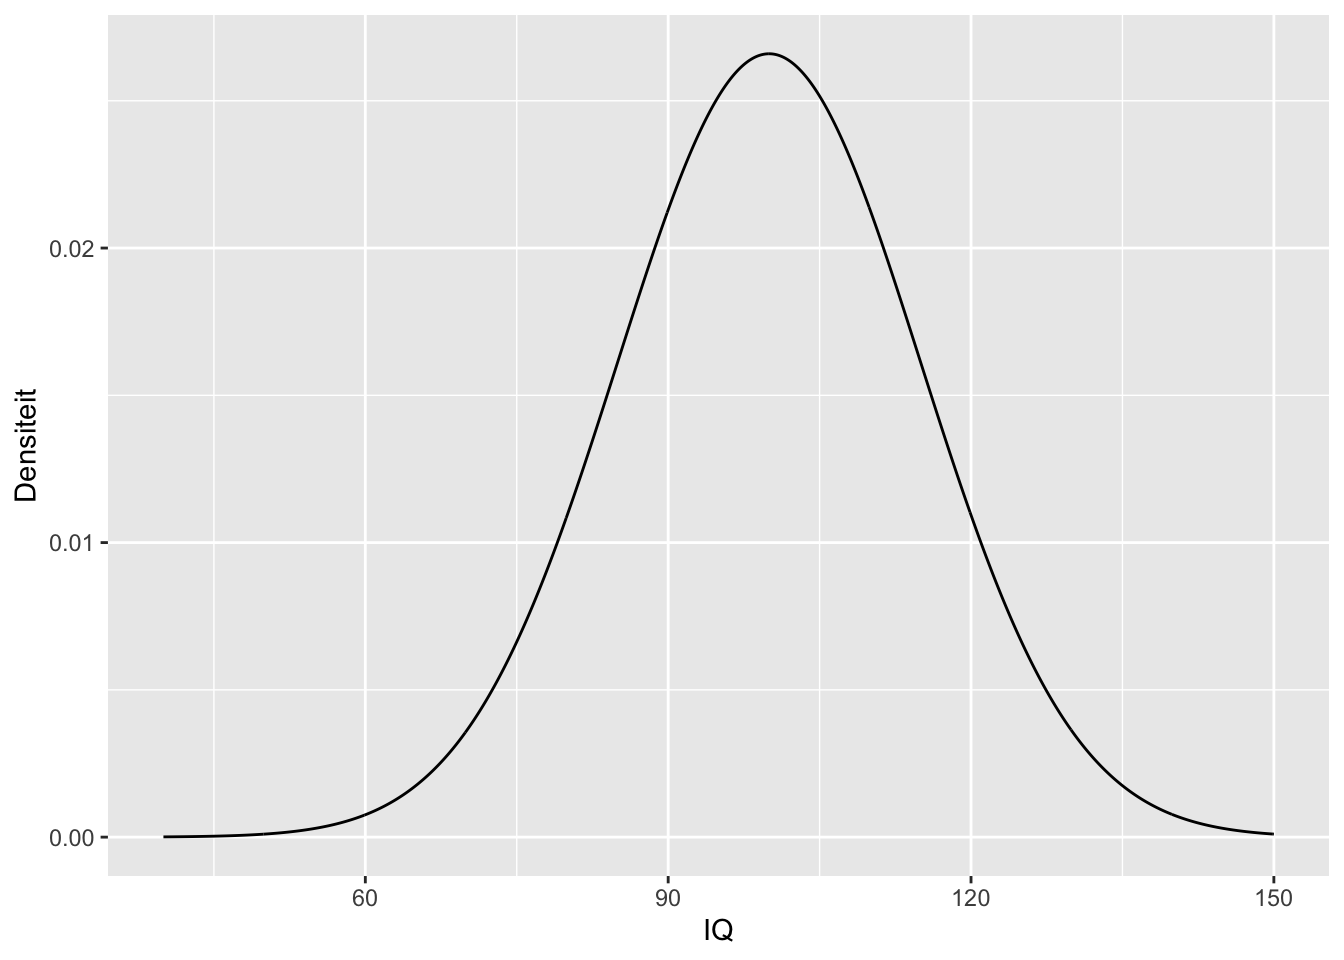
\includegraphics{Statistiek_2020_2021_files/figure-latex/IQ-1} \end{center}

Binnen bepaalde grenzen kunnen continue toevallig veranderlijken alle mogelijke waarden aannemen dus is \(\Omega\) oneindig groot.

\hypertarget{cumulatieve-distributie}{%
\paragraph{Cumulatieve distributie}\label{cumulatieve-distributie}}

Opnieuw is de cumulatieve distributie

\[F(X)=Pr(X\leq x).\]

Omdat X continu is berekenen we deze probabiliteit a.d.h.v. een integraal

\[F(x)=\int \limits_{-\infty}^x f(x) dx\]

Merk op dat \(f(x)=0\) als x niet tot de steekproefruimte behoord.

We kunnen \(F(x)\) berekenen voor een normaal verdeelde toevallig veranderlijke met de functie \texttt{pnorm} die opnieuw argumenten \texttt{mean} en \texttt{sd} heeft.

\begin{Shaded}
\begin{Highlighting}[]
\NormalTok{iq }\OperatorTok{\%\textgreater{}\%}\StringTok{ }\KeywordTok{mutate}\NormalTok{(}\DataTypeTok{Probability =} \KeywordTok{pnorm}\NormalTok{(IQ, }\DataTypeTok{mean =} \DecValTok{100}\NormalTok{, }\DataTypeTok{sd =} \DecValTok{15}\NormalTok{)) }\OperatorTok{\%\textgreater{}\%}\StringTok{ }
\StringTok{    }\KeywordTok{ggplot}\NormalTok{(}\KeywordTok{aes}\NormalTok{(}\DataTypeTok{x =}\NormalTok{ IQ, }\DataTypeTok{y =}\NormalTok{ Probability)) }\OperatorTok{+}\StringTok{ }\KeywordTok{geom\_line}\NormalTok{()}
\end{Highlighting}
\end{Shaded}

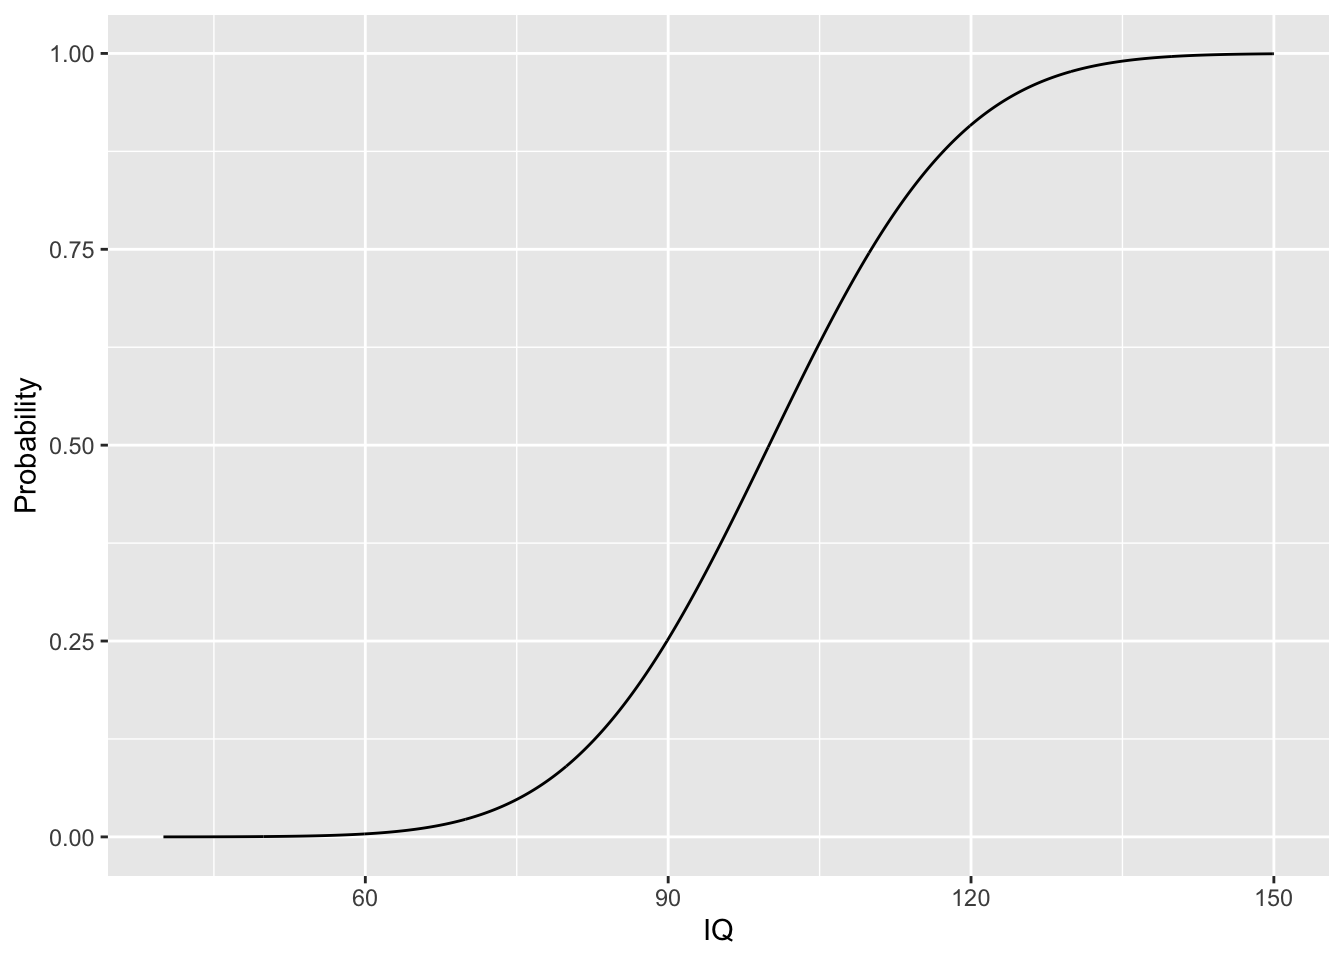
\includegraphics{Statistiek_2020_2021_files/figure-latex/unnamed-chunk-34-1.pdf}

De probabiliteit dat het IQ van een random subject lager is dan 80 wordt in R berekend door

\begin{Shaded}
\begin{Highlighting}[]
\KeywordTok{pnorm}\NormalTok{(}\DecValTok{80}\NormalTok{, }\DataTypeTok{mean =} \DecValTok{100}\NormalTok{, }\DataTypeTok{sd =} \DecValTok{15}\NormalTok{)}
\end{Highlighting}
\end{Shaded}

\begin{verbatim}
## [1] 0.09121122
\end{verbatim}

\begin{center}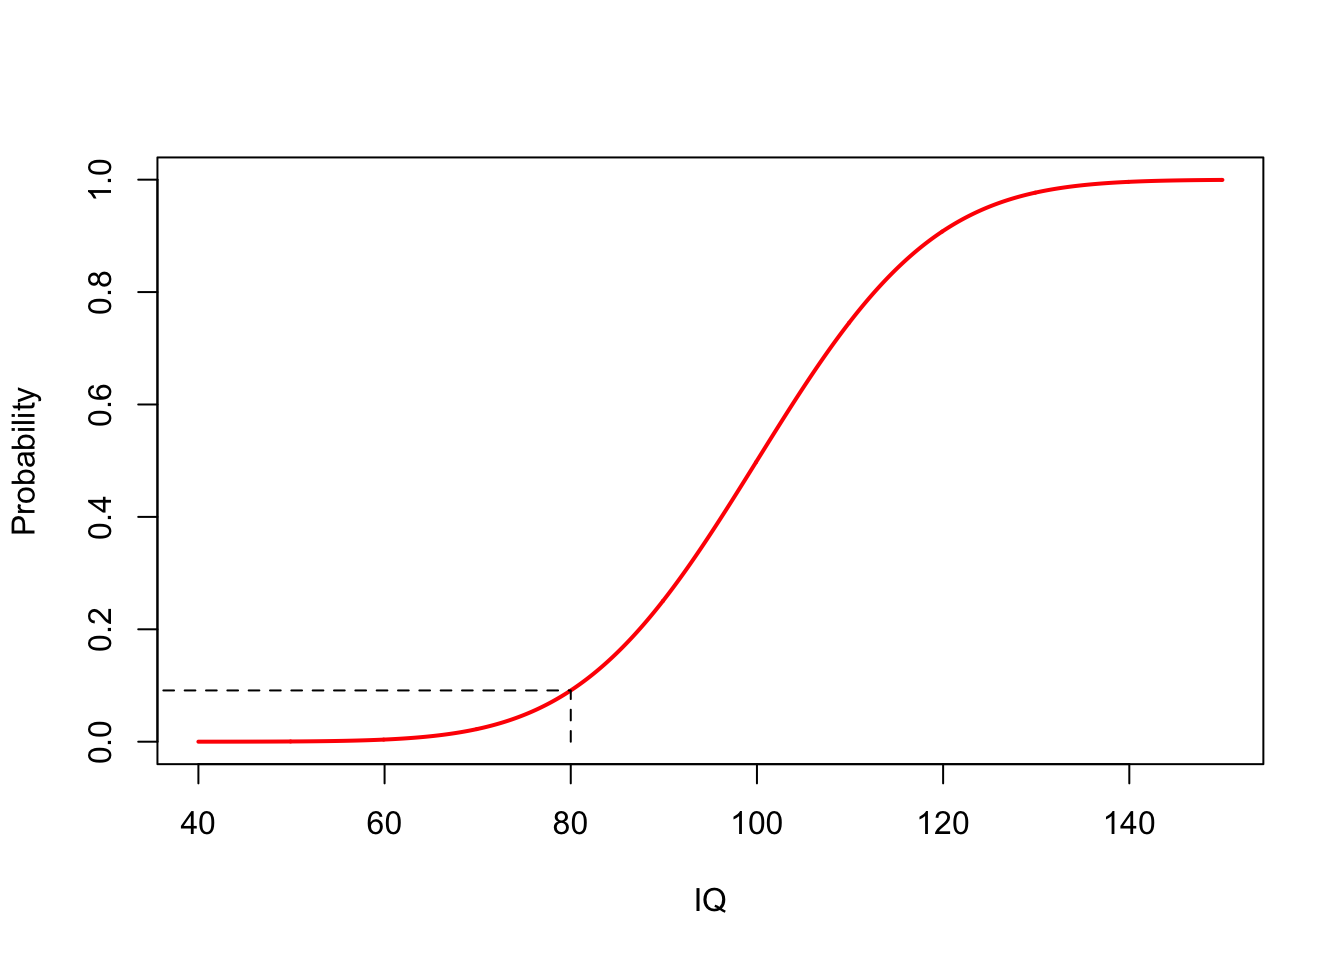
\includegraphics{Statistiek_2020_2021_files/figure-latex/unnamed-chunk-36-1} \end{center}

\begin{center}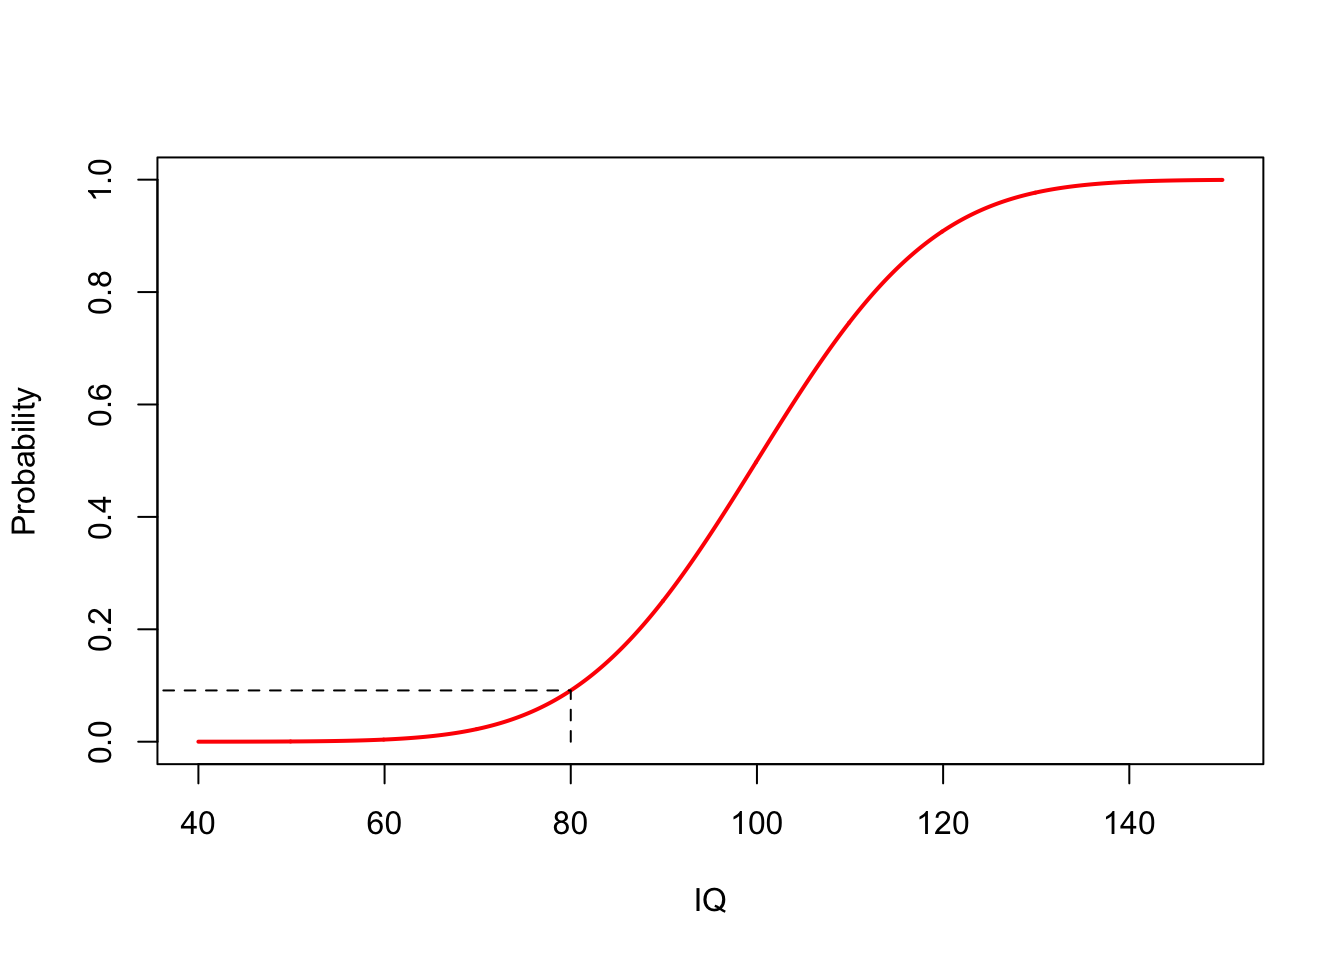
\includegraphics{Statistiek_2020_2021_files/figure-latex/unnamed-chunk-37-1} \end{center}

Voor de grootst mogelijke waarde voor \(X\) integreren we over de volledige steekproefruimte \(\Omega\) dus

\[\int \limits_{x \in \Omega} f(x) dx=1.\]

De oppervlakte onder de dichtheidsfunctie is dus steeds 1!

\hypertarget{gemiddelde-en-variantie}{%
\paragraph{Gemiddelde en variantie}\label{gemiddelde-en-variantie}}

Het gemiddelde of de verwachte waarde is

\[\int \limits_{x \in \Omega} x f(x) dx.\]

Voor de normale distributie

\[\int \limits_{-\infty}^{+\infty} x f(x) dx = \mu.\]

De parameter \(\mu\) is dus het gemiddelde van een Normaal verdeelde veranderlijke X de populatie.

De variance \(E[(X-E[X])^2]\)

\[\int \limits_{x \in \Omega} (x-E[X])^2 f(x) dx\]

Voor de normale distributie bekomen we

\[\int \limits_{-\infty}^{+\infty} (x-\mu)^2 f(x) dx = \sigma^2\]

De parameter \(\sigma^2\) is dus de variantie van een Normaal verdeelde veranderlijke X in de populatie.

Het is vaak moeilijk om de variantie te interpreteren gezien ze niet in de zelfde eenheden staat als het gemiddelde. Daarom werken we vaak met de standaardafwijking (SD):

\[SD=\sqrt{E[(X-E[X])^2]}\]

De standaardafwijking voor de normale distributie, \(\sigma\) heeft de interessante interpretatie dat ongeveer 68\% van de populatie een waarde heeft voor de karakteristiek X binnen het interval van 1 standaardafwijking(\(\sigma\)) rond het gemiddelde:

\[P(\mu-\sigma < X < \mu + \sigma) \approx 0.68\]

\begin{center}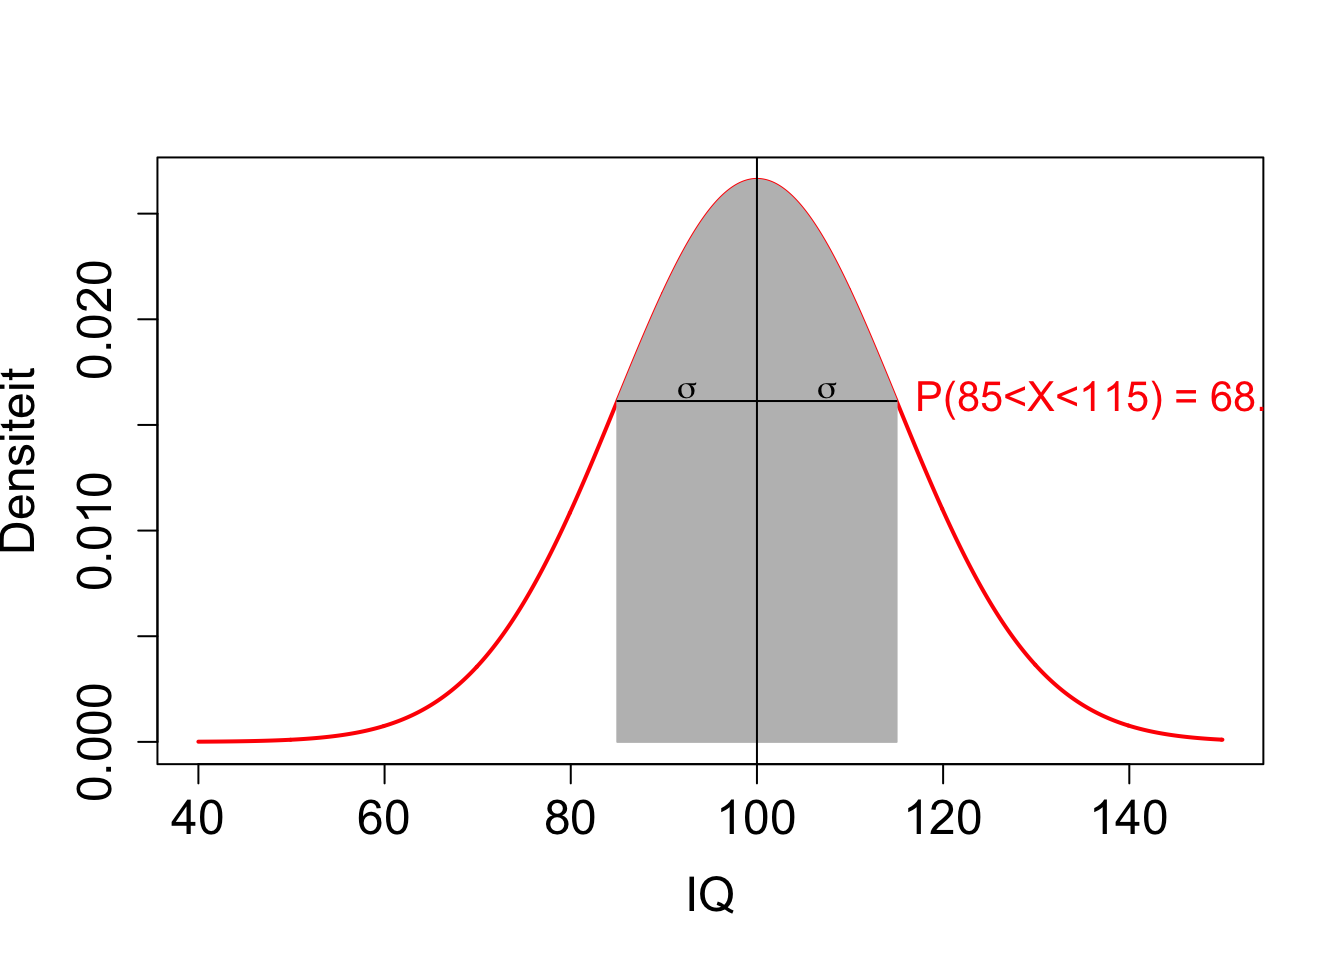
\includegraphics{Statistiek_2020_2021_files/figure-latex/unnamed-chunk-38-1} \end{center}

Voor Normaal verdeelde toevallig veranderlijken heeft ongeveer 95\% van de subjecten in de populatie een waarde die binnen twee standaardafwijkingen (\(2 \sigma\)) ligt van het gemiddelde.

\[P[\mu - 2 \sigma < X < \mu + 2 \sigma]\approx 0.95\]

\begin{center}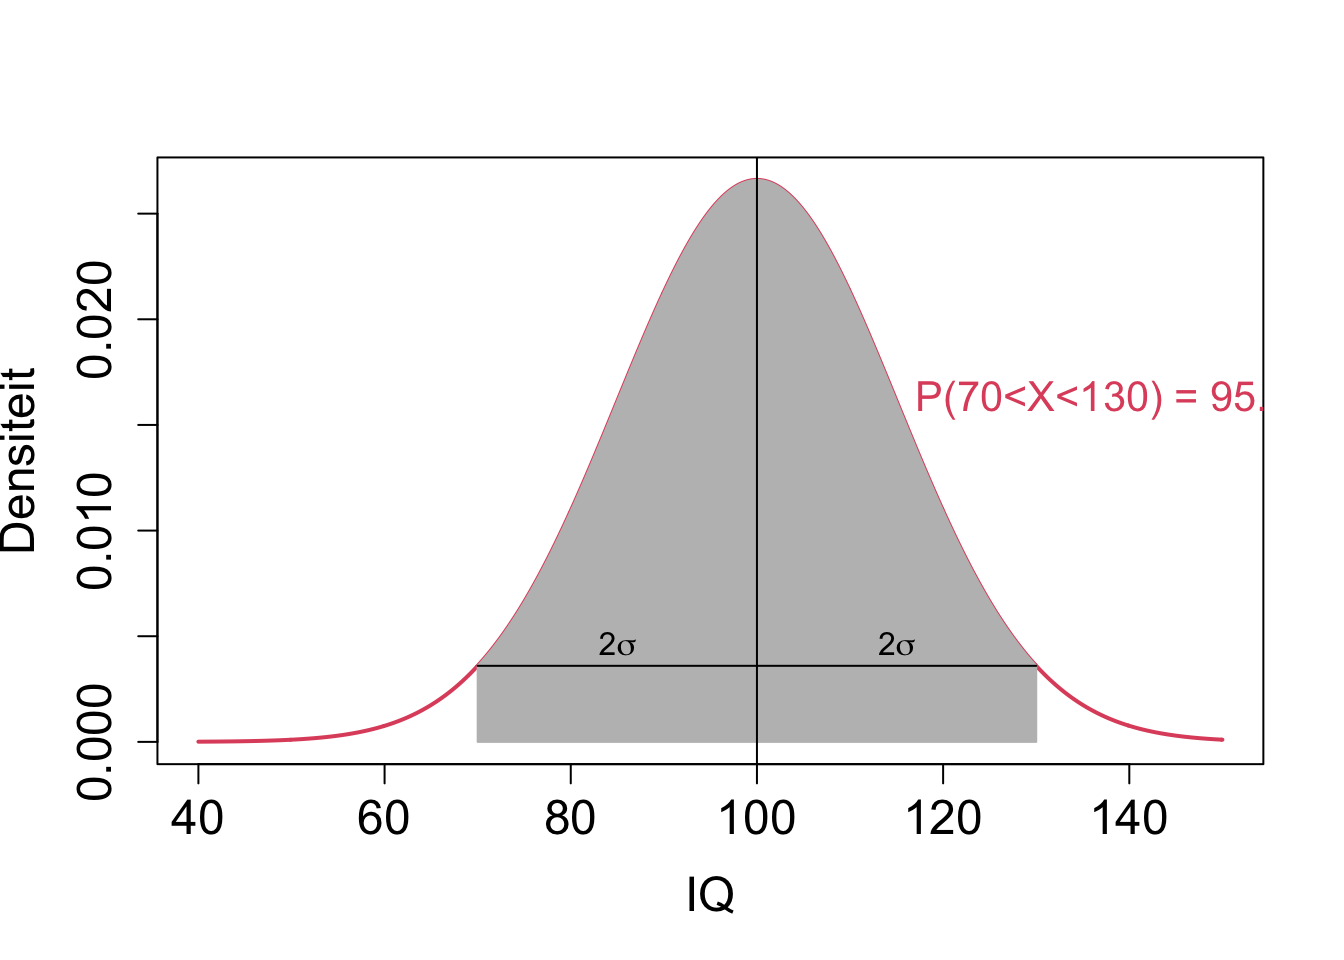
\includegraphics{Statistiek_2020_2021_files/figure-latex/unnamed-chunk-39-1} \end{center}

Deze intervallen worden ook wel een referentie interval genoemd.

\hypertarget{standardisatie}\) en \(z_{97.5\%}\) die respectievelijk corresponderen met \(F(z_{2.5\%})=0.025\) en \(F(z_{97.5\%})=0.975\).

\begin{Shaded}
\begin{Highlighting}[]
\KeywordTok{qnorm}\NormalTok{(}\FloatTok{0.025}\NormalTok{)}
\end{Highlighting}
\end{Shaded}

\begin{verbatim}
## [1] -1.959964
\end{verbatim}

\begin{Shaded}
\begin{Highlighting}[]
\KeywordTok{qnorm}\NormalTok{(}\FloatTok{0.975}\NormalTok{)}
\end{Highlighting}
\end{Shaded}

\begin{verbatim}
## [1] 1.959964
\end{verbatim}

Voor een standaard Normaal verdeelde toevallig veranderlijke valt inderdaad ongeveer \(0.975 - 0.025=0.95\) van de waarden binnen het interval {[}-2,2{]}, of binnen 2 standaardafwijkingen (\(\sigma=1\)) van het gemiddelde (\(\mu=0\)).

\hypertarget{subsec:normalcalc}{%
\subsection{Achtergrond Normale verdeling}\label{subsec:normalcalc}}

De \emph{Normale curve} of \emph{Normale dichtheidsfunctie} wordt gegeven door:

\begin{equation*}
f(x) = \frac{1}{\sigma \sqrt{2 \pi} } \exp \left ( - \frac{ (x - \mu)^2 }{ 2
\sigma^2} \right ).
\end{equation*}

Ze wordt beschreven door 2 onbekende parameters \(\mu\) en \(\sigma\), waarbij \(\mu\) het gemiddelde van de verdeling van de observaties aangeeft en \(\sigma\)
de standaarddeviatie. Deze curve geeft voor elke waarde \(x\) weer hoe
frequent deze waarde, relatief gezien, voorkomt. De notatie \(\pi\) verwijst
naar het getal \(\pi=3.1459...\) Wanneer het gemiddelde 0 is en de variantie
1, spreekt men van de \emph{standaardnormale curve} of \emph{standaardnormale dichtheidsfunctie}.

Een lukrake observatie uit een reeks gegevens wiens verdeling de Normale
curve volgt, wordt een \textbf{Normaal verdeelde observatie} genoemd.
Dergelijke observaties komen frequent voor: voor heel wat reeksen gegevens
die symmetrisch verdeeld zijn, vormt de Normale curve met \(\mu\) gelijk aan \(\bar x\) en \(\sigma\) gelijk aan \(s_x\) immers een goede benadering voor het
histogram.

Voor Normaal verdeelde gegevens geeft de oppervlakte onder de Normale curve
tussen 2 willekeurige getallen \(a\) en \(b\) het percentage van de
observaties weer dat tussen deze 2 getallen gelegen is. Op die manier laat de
Normale curve toe om, enkel op basis van kennis van het gemiddelde en de
standaarddeviatie, na te gaan welk percentage van de gegevens bij benadering
tussen 2 willekeurige getallen \(a\) en \(b\) gelegen is.

Om deze berekening uit te voeren, gaan we als volgt te werk. Zij \(X\) een
lukrake meting uit een reeks Normaal verdeelde gegevens met gemiddelde \(\mu\)
en standaarddeviatie \(\sigma\). Dan noteren we met \(P(X\leq b)\) de
oppervlakte onder de Normale curve die links van \(b\) gelegen is, en met \(P(a\leq X\leq b)\) de oppervlakte onder de Normale curve tussen \(a\) en \(b\).
Hierbij is\footnote{Hierbij maken we gebruik van het feit dat voor een Normaal verdeelde observatie \(X\), \(P(X=a)=0\) voor elk reëel getal \(a\), zodat \(P(X\leq a)=P(X<a)\).}

\begin{equation*}
P(a\leq X\leq b)=P(X\leq b)-P(X\leq a)
\end{equation*}

Om \(P(a\leq X\leq b)\) te berekenen, hebben we dus enkel een strategie nodig
om voor een willekeurig getal \(x\), het getal \(F(x) = P(X \leq x)\) uit te
rekenen. Dit staat uitgezet in functie van \(x\) in Figuur \ref{fig:continu}
(rechtsboven) voor \(\mu=80\) en \(\sigma=12\) en wordt een \emph{distributiefunctie} genoemd.

\begin{definition}[distributiefunctie]
\protect\hypertarget{def:unnamed-chunk-41}{}{\label{def:unnamed-chunk-41} \iffalse (distributiefunctie) \fi{} }
\end{definition}
De functie die voor elk getal \(x\) uitdrukt wat de kans is dat een lukrake
meting \(X\) met gekende verdeling (bvb. een Normale verdeling) kleiner of
gelijk is aan \(x\), wordt de \textbf{distributiefunctie} van die verdeling
genoemd.

\textbf{Einde definitie}

Omdat de Normale dichtheidsfunctie zeer complex is, blijkt dat het getal \(F(x)\) niet expliciet uit te rekenen is. Om die reden heeft men de getallen \(F(x)\)
voor de standaardnormale verdelingsfunctie getabuleerd. Voor
deze standaardnormale curve duidt men voor een willekeurige waarde \(z\), het
getal \(F(z)\) met \(\Phi(z)\) aan. Omwille van de symmetrie rond 0 van de
standaardnormale curve kan de waarde van \(\Phi(-z)\) dan uit de waarde van \(\Phi(z)\) worden afgeleid als

\begin{equation*}
\Phi(-z)= 1- \Phi(z)
\end{equation*}

Deze uitdrukking geeft aan dat voor een reeks standaardnormaal verdeelde
metingen, het percentage dat kleiner is dan \(-z\) gelijk is aan
het percentage dat groter is dan \(z\).

Om nu \(P(a\leq X\leq b)\) te berekenen op basis van de tabellen voor de
standaardnormale verdeling gaan we als volgt te werk. Vooreerst kan men
aantonen dat het resultaat van een lineaire transformatie \(aX+b\) op een
Normaal verdeelde meting \(X\) met gemiddelde \(\mu\) en standaarddeviatie \(\sigma\) terug een Normaal verdeelde meting toevalsveranderlijke is, maar nu
met gemiddelde \(a\mu+b\) en standaarddeviatie \(|a|\sigma\). Op die manier kan
men elke Normaal verdeelde meting met gemiddelde \(\mu\) en standaarddeviatie \(\sigma\) omzetten naar een standaardnormale meting door ze als volgt te
\emph{standaardiseren}:

\begin{equation*}
Z = \frac{X- \mu}{\sigma}
\end{equation*}

Verifieer dat \(Z\) inderdaad gemiddelde 0 en standaarddeviatie 1 heeft!

Aangezien voor een willekeurig getal \(x\)

\begin{equation*}
X\leq x \Leftrightarrow \frac{X-\mu}{\sigma} \leq \frac{x-\mu}{\sigma}
\end{equation*}

vinden we nu dat

\begin{eqnarray*}
P(a \leq X \leq b) & = & P\left(\frac{a-\mu}{\sigma} \leq Z \leq \frac{b-\mu%
}{\sigma} \right) \\
& = & \Phi \left (\frac{b-\mu}{\sigma} \right ) - \Phi \left (\frac{a-\mu}{%
\sigma} \right )
\end{eqnarray*}

De getallen \(\Phi \left (\frac{b-\mu}{\sigma} \right )\) en \(\Phi \left (\frac{a-\mu}{\sigma} \right )\) kunnen hierbij rechtstreeks uit tabellen of R software worden gehaald. In het vervolg zullen we
algemeen de notatie \(Z\) gebruiken om een standaardnormaal verdeelde meting
aan te duiden.

\begin{exercise}
\protect\hypertarget{exr:unnamed-chunk-42}{}{\label{exr:unnamed-chunk-42} }
\end{exercise}
Een labo bepaalt in een visstaal Hg via een methode op basis van AAS. In
werkelijkheid bevat het staal (gemiddeld) 1.90 ppm. De meetmethode is echter
niet perfect, zoals aangegeven door een standaarddeviatie van 0.10 ppm. Wat
is de kans dat de laborant die het staal onderzoekt, een meetresultaat van
2.10 ppm of meer vaststelt?

Om op deze vraag te antwoorden, noteren we met \(X\) het meetresultaat van de
laborant en berekenen we

\begin{eqnarray*}
P(X\geq 2)&=&P\left(\frac{X-\mu}{\sigma}\geq \frac{2.1-1.9}{0.1}\right) \\
&=&P(Z\geq 2) = 2.28\%
\end{eqnarray*}

We besluiten dat er 2.28\% kans is dat de laborant een meetresultaat van
minstens 2.10 ppm zal vaststellen. In R kan dit resultaat als volgt bekomen worden:

\begin{Shaded}
\begin{Highlighting}[]
\DecValTok{1} \OperatorTok{{-}}\StringTok{ }\KeywordTok{pnorm}\NormalTok{(}\FloatTok{2.1}\NormalTok{, }\DataTypeTok{mean =} \FloatTok{1.9}\NormalTok{, }\DataTypeTok{sd =} \FloatTok{0.1}\NormalTok{)}
\end{Highlighting}
\end{Shaded}

\begin{verbatim}
## [1] 0.02275013
\end{verbatim}

waarbij de functie pnorm de distributiefunctie van de Normale verdeling voorstelt.

\textbf{Einde oefening}

Met \(z_{\alpha}\) duiden\footnote{Let wel op want in verschillende boeken krijgt het symbool \(z_{\alpha}\) verschillende definities!} we die waarde aan waar \(\alpha100\%\) van de
oppervlakte onder de standaardnormale curve rechts van zit; m.a.w. waarvoor
geldt dat \(P(Z \geq z_{\alpha}) = \alpha\). Als \(Z\) een standaardnormaal
verdeelde meting is, dan stelt \(z_{\alpha}\) bijgevolg het \((1-\alpha)100\%\)
percentiel van die verdeling voor. Voor \(z_{\alpha/2}\) geldt dat \(P(-z_{\alpha/2}\leq Z \leq z_{\alpha/2}) = 1-\alpha\). Bijvoorbeeld, \(P( - z_{0.025}\leq Z \leq z_{0.025}) = 95\%\). Voor een reeks standaardnormaal
verdeelde metingen bevat het interval \([-z_{\alpha/2},z_{\alpha/2}]\) dus \((1-\alpha)100\%\) van de observaties.

Stel dat \(X\) een Normaal verdeelde meting is met gemiddelde \(\mu\) en
standaarddeviatie \(\sigma\). Dan geldt dat

\begin{equation*}
P\left( - z_{\alpha/2}\leq \frac{X - \mu}{\sigma} \leq z_{\alpha/2}\right) =
1-\alpha .
\end{equation*}

Hieruit volgt dat

\begin{equation*}
P( \mu - z_{\alpha/2} \sigma \leq X \leq \mu + z_{\alpha/2} \sigma ) =
1-\alpha .
\end{equation*}

Voor een reeks Normaal verdeelde metingen met gemiddelde \(\mu\) en
standaarddeviatie \(\sigma\) bevat het interval \([\mu-z_{\alpha/2}\sigma,\mu+z_{\alpha/2}\sigma]\) dus \((1-\alpha)100\%\) van de observaties. In de
praktijk worden de parameters \(\mu\) en \(\sigma\) hierbij vervangen door \(\bar x\) en \(s_x\).

Het resulterende interval \([\bar x-z_{\alpha/2}s_x,\bar x+z_{\alpha/2}s_x]\)
wordt vaak gebruikt\footnote{Dit interval bevat niet exact \((1-\alpha)100\%\) van de observaties, maar slechts bij benadering, omdat het geen rekening houdt met het feit dat \(\bar x\) en \(\sigma_x\) impreciese schattingen zijn voor \(\mu\) en \(\sigma\) op basis van een eindige steekproef. Meer accurate referentie-intervallen die deze imprecisie in rekening brengen, ook predictie-intervallen genoemd}, o.a. in de klinische chemie, om \emph{referentie-intervallen} te berekenen voor een test ter opsporing van een
bepaalde pathologie. Eenmaal zo'n referentie-interval, ook wel \emph{normaal interval} genoemd, werd bepaald, wordt het testresultaat van een
patiënt met de vermoede pathologie vergeleken met het interval. Een
resultaat buiten het interval is dan indicatief voor de aanwezigheid van de
pathologie.

Bij het bepalen van referentie-intervallen is het noodzakelijk om de methode
eerst te testen bij mensen zonder de pathologie in kwestie. Voor dit doel
worden `normale en gezonde vrijwilligers' aangezocht. Vaak worden hiertoe
collega's genomen uit het laboratorium dat de test heeft ontwikkeld, hoewel
dit allesbehalve ideaal is. Immers, mensen die in een zelfde laboratorium
werken, zijn blootgesteld aan dezelfde werkomgeving, die op zijn beurt een
invloed kan hebben op hun bloedsamenstelling. Bijgevolg is de
bloedsamenstelling van de studiepersonen mogelijks niet representatief voor
een normale, gezonde populatie, hetgeen kan leiden tot vertekende
referentie-intervallen. In deze cursus zullen we een referentie-interval
meer algemeen als volgt definiëren.

\begin{definition}[referentie-interval]
\protect\hypertarget{def:unnamed-chunk-44}{}{\label{def:unnamed-chunk-44} \iffalse (referentie-interval) \fi{} }
\end{definition}
Een \textbf{\((1-\alpha)100\%\) referentie-interval}
voor een veranderlijke \(X\) (bvb. albumine-concentratie
in het bloed) in een gegeven studiepopulatie (bvb. volwassen Belgen onder de
60 jaar) is een interval dat zó gekozen werd dat het met \((1-\alpha)100\%\)
kans de observatie voor een lukraak individu uit die populatie bevat. Voor
een Normaal verdeelde veranderlijke \(X\) met gemiddelde \(\mu\) en
standaarddeviatie \(\sigma\) kan dit berekend worden als

\begin{equation*}
[\mu-z_{\alpha/2}\sigma,\mu+z_{\alpha/2}\sigma]
\end{equation*}

en geschat worden op basis van een lukrake steekproef als

\begin{equation*}
[\bar x-z_{\alpha/2}s_x,\bar x+z_{\alpha/2}s_x]
\end{equation*}

\textbf{Einde definitie}

\hypertarget{steekproef}{%
\section{Steekproef}\label{steekproef}}

In echte studies kennen we de verdeling in de populatie typisch niet!
In de praktijk is het om financiële en logistieke redenen bijna nooit mogelijk om de
volledige populatie te bestuderen. Populatieparameters (v.b. gemiddeld IQ, variantie van IQ) kunnen daarom meestal
niet exact bepaald worden. Enkel een deel van de populatie kan onderzocht
worden, hetgeen men de \emph{steekproef} noemt. Volgens een
gestructureerd design worden daartoe \textbf{lukraak subjecten} uit de doelpopulatie
getrokken en geobserveerd. De onbekende parameters worden vervolgens geschat
o.b.v. die steekproef en noemt met schattingen. In de praktijk hoopt men uiteraard dat de schattingen die men bekomt op basis van de steekproef vergelijkbaar zijn met de overeenkomstige populatieparameters die men voor de volledige populatie zou bekomen.

Stel bijvoorbeeld dat we op basis van de NHANES studie de lengte van volgroeide vrouwen en mannen wensen te bestuderen.
Telkens een lukraak individu getrokken wordt uit de populatie zal men een
realisatie van de toevalsveranderlijke \(X\) kunnen observeren. Die realisatie
of geobserveerde waarde duiden we aan met een kleine letter \(x\). Deze stelt
dus een welbepaald getal voor en is niet langer een onbekende veranderlijke
zoals \(X\). Samengevat zijn de nog onbekende waarden voor de
bestudeerde populatiekarakteristiek bij subjecten 1 tot \(n\) in de
steekproef, toevalsveranderlijken die we algemeen met \(X_1,...,X_n\)
zullen noteren. Na het trekken van de steekproef, ziet men de gerealiseerde
uitkomsten \(x_1, x_2, \dots, x_n\), bijvoorbeeld hun gemeten lengte.

De distributie in de populatie is ongekend en moet worden geschat op basis van de steekproef. Als we aannemen dat de gegevens een bepaalde distributie volgen (b.v. de normale verdeling \(N(\mu,\sigma^2)\)) dan moeten we enkel de populatie parameters (\(\mu\) en \(\sigma^2\)) schatten op basis van de steekproef. We noemen dit schattingen (engels: estimates) en noteren ze als volgt: \(\hat \mu\) en \(\hat \sigma^2\).

\emph{Samenvatting}

\begin{itemize}
\item
  Voor we het experiment uitvoeren is de populatie karakteristiek voor de proefpersonen \(1,\ldots,n\) die we uit de populatie zullen trekken ongekend en zijn dat toevallig veranderlijken: \(X_1, \ldots, X_n\)
\item
  Dit is noodzakelijk om te kunnen redeneren over hoe de resultaten van steekproef tot steekproef kunnen wijzigen
\item
  In een steekproef observeren we gerealiseerde uitkomsten \(x_1, x_2, \dots, x_n\): v.b. gender of lengte van subjecten in de steekproef.
\end{itemize}

\hypertarget{nhanes-gender}{%
\section{NHANES: Gender}\label{nhanes-gender}}

\begin{Shaded}
\begin{Highlighting}[]
\KeywordTok{library}\NormalTok{(NHANES)}
\NormalTok{NHANES }\OperatorTok{\%\textgreater{}\%}\StringTok{ }\KeywordTok{ggplot}\NormalTok{(}\KeywordTok{aes}\NormalTok{(}\DataTypeTok{x =}\NormalTok{ Gender)) }\OperatorTok{+}\StringTok{ }\KeywordTok{geom\_bar}\NormalTok{()}
\end{Highlighting}
\end{Shaded}

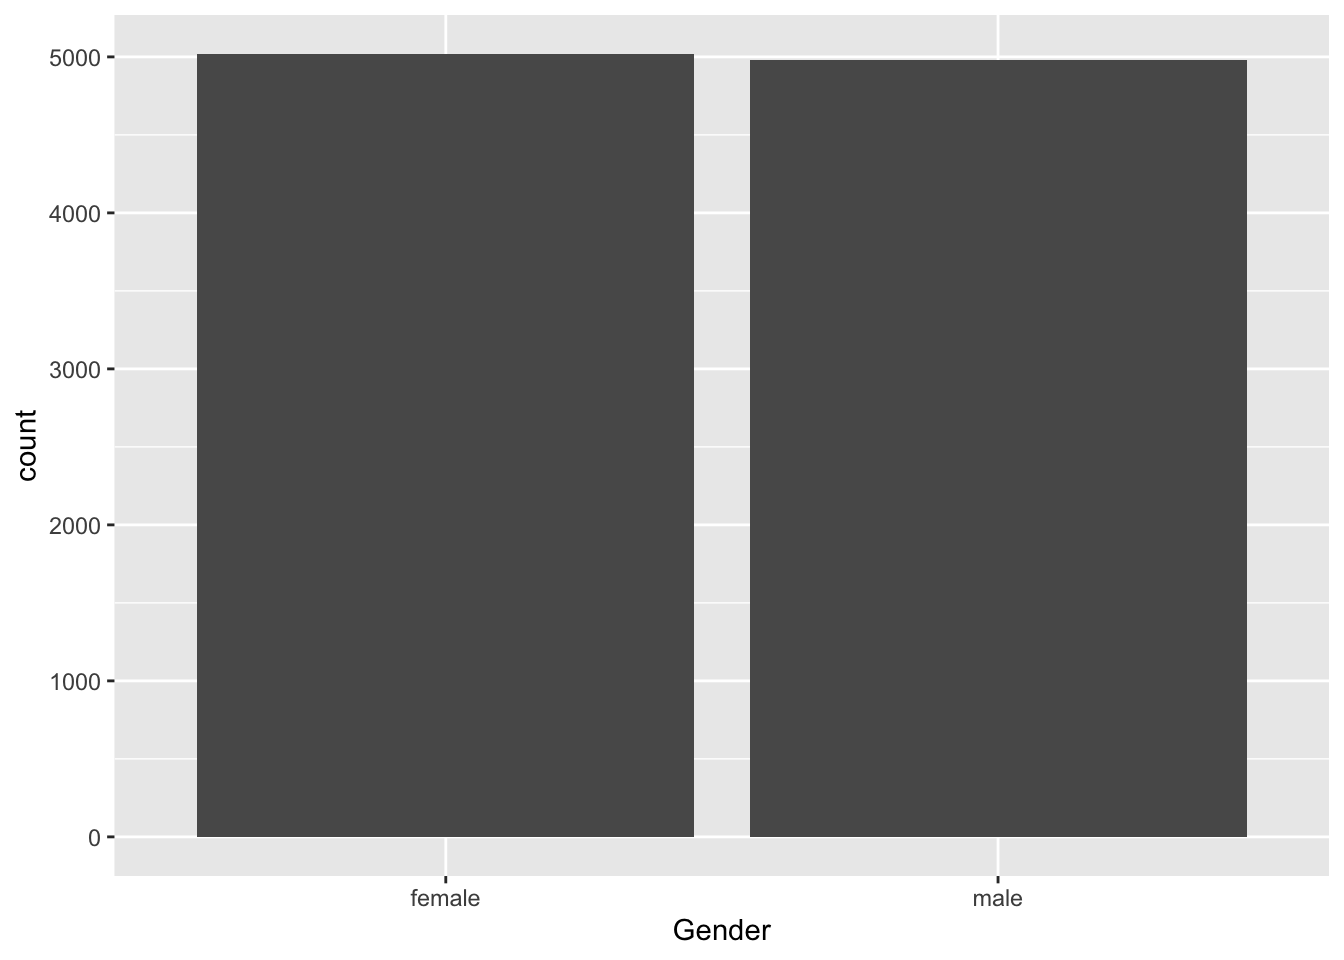
\includegraphics{Statistiek_2020_2021_files/figure-latex/unnamed-chunk-45-1.pdf}

\begin{itemize}
\tightlist
\item
  Gender is een binaire variabele.
\item
  Het volgt een Bernoulli distibutie.
\item
  De Bernoulli distributie heeft een parameter: het gemiddelde \(\pi\).
\item
  We kunnen \(\pi\) schatten op basis van de steekproef door het steekproefgemiddelde te berekenen \(\bar x = \sum\limits_{i=1}^n x_i\)
\item
  Merk op dat het steekproefgemiddelde zelf een toevallig veranderlijke is! Het wijzigt ook van steekproef tot steekproef!
\end{itemize}

\begin{Shaded}
\begin{Highlighting}[]
\NormalTok{NHANES }\OperatorTok{\%\textgreater{}\%}\StringTok{ }\KeywordTok{count}\NormalTok{(Gender) }\OperatorTok{\%\textgreater{}\%}\StringTok{ }\KeywordTok{mutate}\NormalTok{(}\DataTypeTok{probability =}\NormalTok{ n}\OperatorTok{/}\KeywordTok{sum}\NormalTok{(n))}
\end{Highlighting}
\end{Shaded}

\begin{verbatim}
## # A tibble: 2 x 3
##   Gender     n probability
##   <fct>  <int>       <dbl>
## 1 female  5020       0.502
## 2 male    4980       0.498
\end{verbatim}

\hypertarget{nhanes-lengte}{%
\section{NHANES: Lengte}\label{nhanes-lengte}}

\hypertarget{empirische-distributie}{%
\subsection{Empirische distributie}\label{empirische-distributie}}

We kunnen de distributie van de lengte voor volwassen vrouwen schatten aan de hand van het histogram.

\begin{Shaded}
\begin{Highlighting}[]
\NormalTok{NHANES }\OperatorTok{\%\textgreater{}\%}\StringTok{ }\KeywordTok{filter}\NormalTok{(Gender }\OperatorTok{==}\StringTok{ "female"} \OperatorTok{\&}\StringTok{ }\OperatorTok{!}\KeywordTok{is.na}\NormalTok{(Height) }\OperatorTok{\&}\StringTok{ }
\StringTok{    }\NormalTok{Age }\OperatorTok{\textgreater{}}\StringTok{ }\DecValTok{18}\NormalTok{) }\OperatorTok{\%\textgreater{}\%}\StringTok{ }\KeywordTok{ggplot}\NormalTok{(}\KeywordTok{aes}\NormalTok{(}\DataTypeTok{x =}\NormalTok{ Height)) }\OperatorTok{+}\StringTok{ }\KeywordTok{geom\_histogram}\NormalTok{()}
\end{Highlighting}
\end{Shaded}

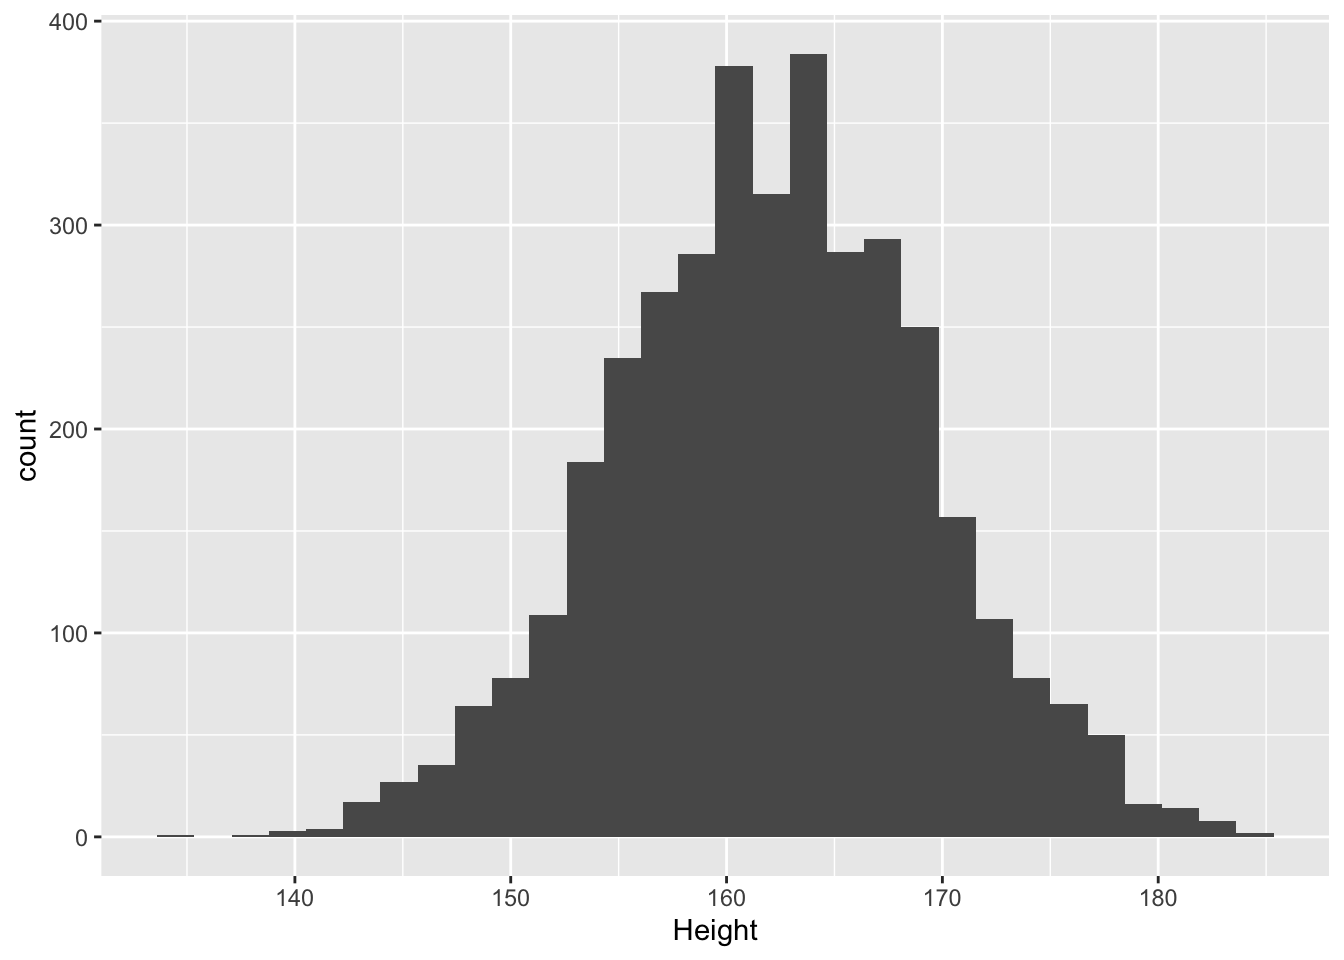
\includegraphics{Statistiek_2020_2021_files/figure-latex/unnamed-chunk-47-1.pdf}

We kunnen de cumulative distributie functie schatten door gebruik te maken van de empirische cumulatieve distributie functie.
- Elke observatie werd één keer geobserveerd in het staal.
- Dus empirische cumulatieve distributie functie van het staal is een discrete distributie met probabiliteit 1/n op elke observatie.
- De empirische cumulatieve distributie functie (ECDF) is gegeven door

\begin{verbatim}
$$ECDF(x) = \sum\limits_{x_i \leq x} \frac{1}{n} = \frac{\# (x_i \leq x)}{n}$$
\end{verbatim}

\begin{Shaded}
\begin{Highlighting}[]
\NormalTok{NHANES }\OperatorTok{\%\textgreater{}\%}\StringTok{ }\KeywordTok{filter}\NormalTok{(Gender }\OperatorTok{==}\StringTok{ "female"} \OperatorTok{\&}\StringTok{ }\OperatorTok{!}\KeywordTok{is.na}\NormalTok{(Height) }\OperatorTok{\&}\StringTok{ }
\StringTok{    }\NormalTok{Age }\OperatorTok{\textgreater{}}\StringTok{ }\DecValTok{18}\NormalTok{) }\OperatorTok{\%\textgreater{}\%}\StringTok{ }\KeywordTok{ggplot}\NormalTok{(}\KeywordTok{aes}\NormalTok{(}\DataTypeTok{x =}\NormalTok{ Height)) }\OperatorTok{+}\StringTok{ }\KeywordTok{stat\_ecdf}\NormalTok{()}
\end{Highlighting}
\end{Shaded}

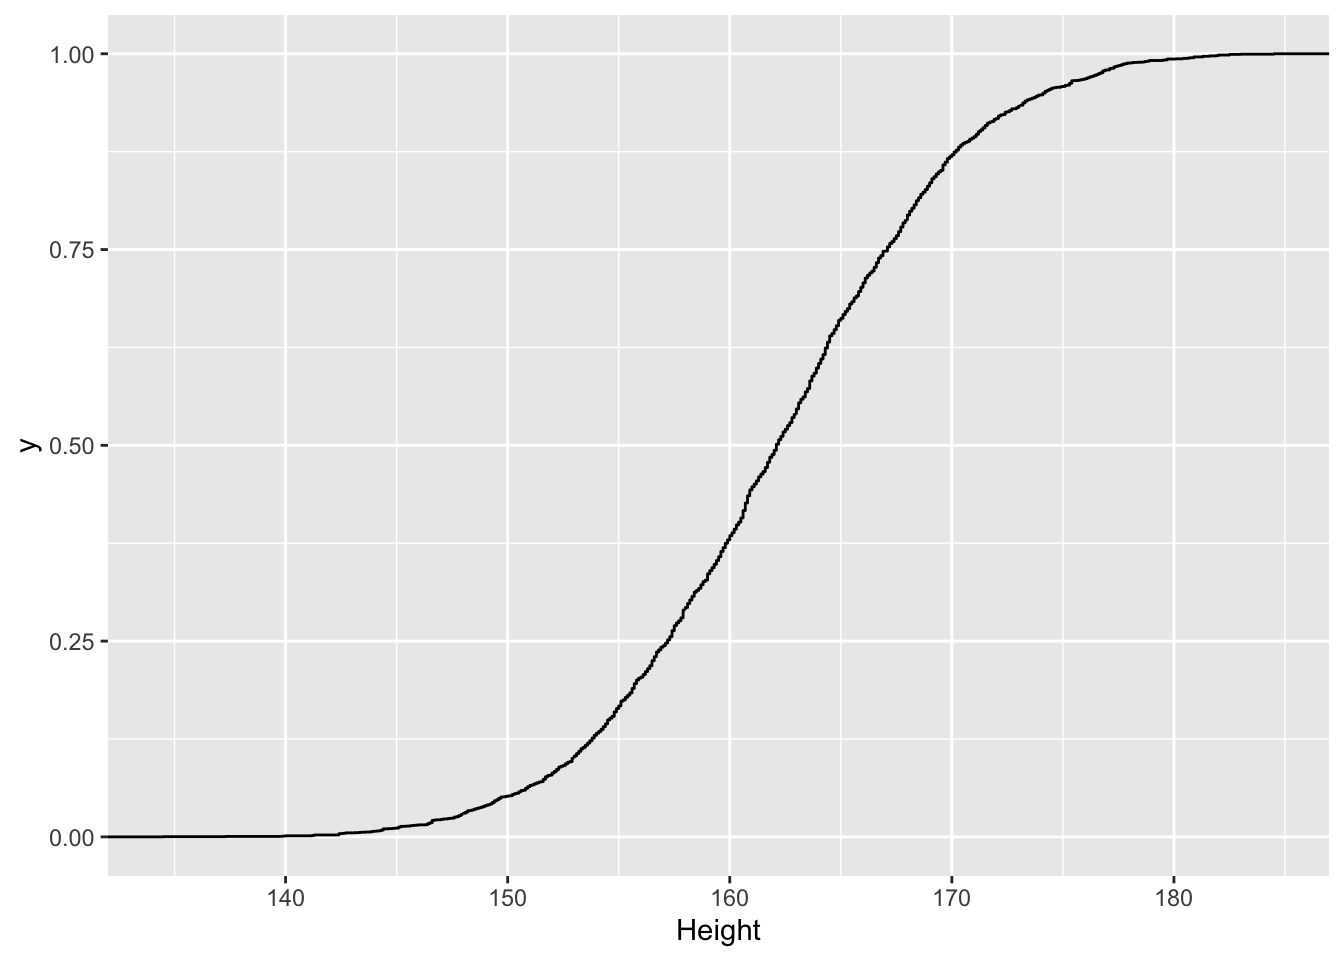
\includegraphics{Statistiek_2020_2021_files/figure-latex/unnamed-chunk-48-1.pdf}

We kunnen de empische cumulatieve distributie functie gebruiken om kansen te berekenen.
Wat is de kans dat een vrouw kleiner is dan 150 cm.

\begin{Shaded}
\begin{Highlighting}[]
\NormalTok{ecdfFem \textless{}{-}}\StringTok{ }\NormalTok{NHANES }\OperatorTok{\%\textgreater{}\%}\StringTok{ }\KeywordTok{filter}\NormalTok{(Gender }\OperatorTok{==}\StringTok{ "female"} \OperatorTok{\&}\StringTok{ }\OperatorTok{!}\KeywordTok{is.na}\NormalTok{(Height) }\OperatorTok{\&}\StringTok{ }
\StringTok{    }\NormalTok{Age }\OperatorTok{\textgreater{}}\StringTok{ }\DecValTok{18}\NormalTok{) }\OperatorTok{\%\textgreater{}\%}\StringTok{ }\KeywordTok{pull}\NormalTok{(}\StringTok{"Height"}\NormalTok{) }\OperatorTok{\%\textgreater{}\%}\StringTok{ }\NormalTok{ecdf}
\KeywordTok{ecdfFem}\NormalTok{(}\DecValTok{150}\NormalTok{)}
\end{Highlighting}
\end{Shaded}

\begin{verbatim}
## [1] 0.05222073
\end{verbatim}

We illustreren dit ook voor een steekproef van grootte 10

\begin{Shaded}
\begin{Highlighting}[]
\KeywordTok{set.seed}\NormalTok{(}\DecValTok{502}\NormalTok{)}
\NormalTok{fem10 \textless{}{-}}\StringTok{ }\NormalTok{NHANES }\OperatorTok{\%\textgreater{}\%}\StringTok{ }\KeywordTok{filter}\NormalTok{(Gender }\OperatorTok{==}\StringTok{ "female"} \OperatorTok{\&}\StringTok{ }\OperatorTok{!}\KeywordTok{is.na}\NormalTok{(Height) }\OperatorTok{\&}\StringTok{ }
\StringTok{    }\NormalTok{Age }\OperatorTok{\textgreater{}}\StringTok{ }\DecValTok{18}\NormalTok{) }\OperatorTok{\%\textgreater{}\%}\StringTok{ }\KeywordTok{sample\_n}\NormalTok{(}\DataTypeTok{size =} \DecValTok{10}\NormalTok{)}

\NormalTok{fem10 }\OperatorTok{\%\textgreater{}\%}\StringTok{ }\KeywordTok{ggplot}\NormalTok{(}\KeywordTok{aes}\NormalTok{(}\DataTypeTok{x =}\NormalTok{ DirectChol)) }\OperatorTok{+}\StringTok{ }\KeywordTok{stat\_ecdf}\NormalTok{()}
\end{Highlighting}
\end{Shaded}

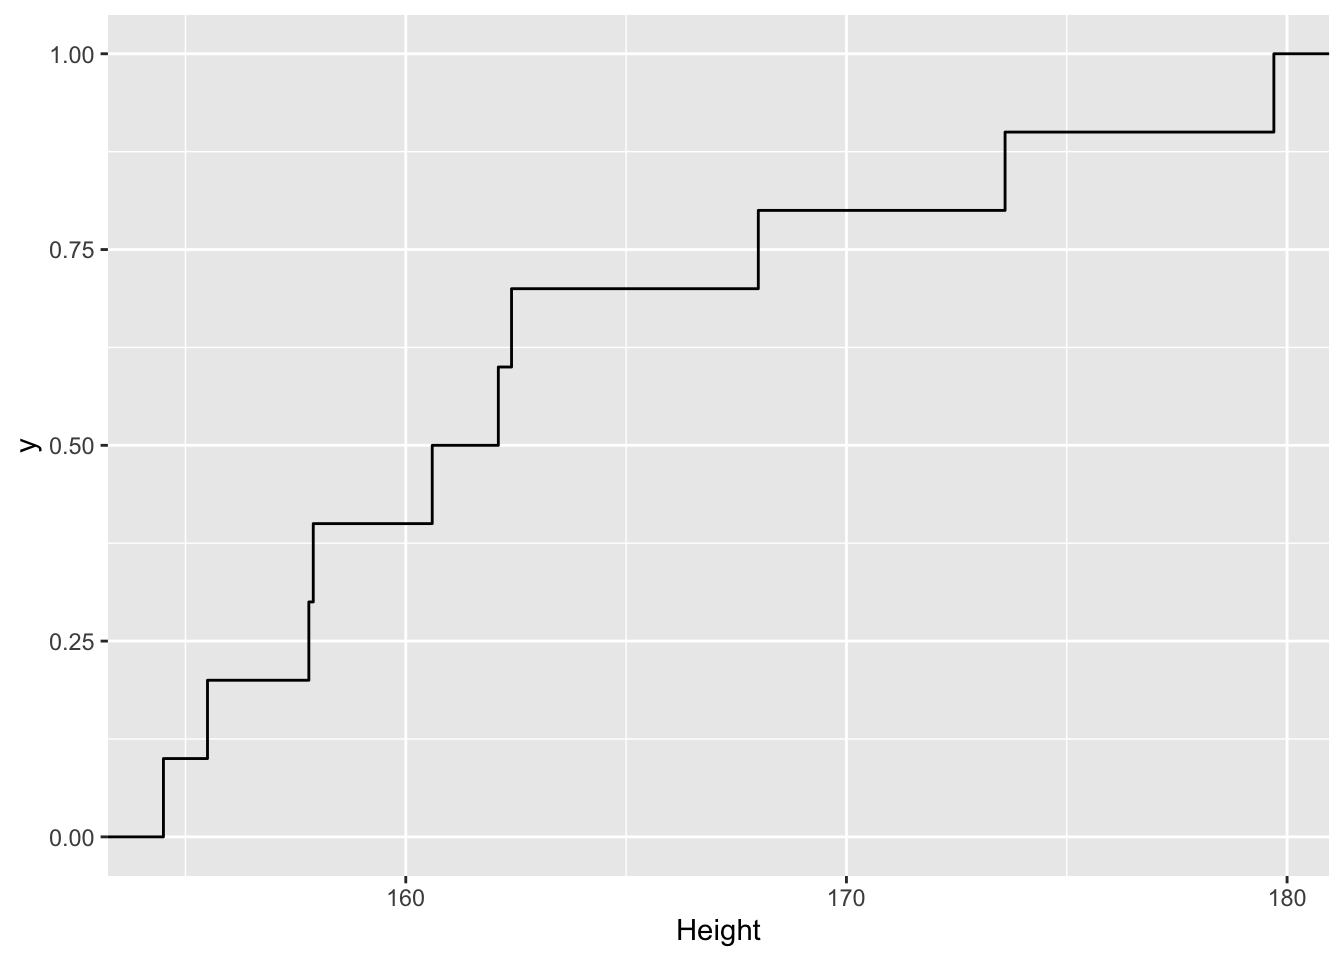
\includegraphics{Statistiek_2020_2021_files/figure-latex/unnamed-chunk-50-1.pdf}

\begin{Shaded}
\begin{Highlighting}[]
\NormalTok{ecdfFem10 \textless{}{-}}\StringTok{ }\NormalTok{fem10 }\OperatorTok{\%\textgreater{}\%}\StringTok{ }\KeywordTok{pull}\NormalTok{(Height) }\OperatorTok{\%\textgreater{}\%}\StringTok{ }\NormalTok{ecdf}
\KeywordTok{ecdfFem10}\NormalTok{(}\DecValTok{150}\NormalTok{)}
\end{Highlighting}
\end{Shaded}

\begin{verbatim}
## [1] 0
\end{verbatim}

Merk op dat die kans niet goed wordt geschat o.b.v. de kleine steekproef. Er zijn immers te weinig observaties om de kansen goed te kunnen schatten.

Merk ook op dat we die kans ook hadden kunnen schatten door te berekenen hoeveel lengtemetingen er lager zijn dan 150.

\begin{Shaded}
\begin{Highlighting}[]
\NormalTok{NHANES }\OperatorTok{\%\textgreater{}\%}\StringTok{ }\KeywordTok{filter}\NormalTok{(Gender }\OperatorTok{==}\StringTok{ "female"} \OperatorTok{\&}\StringTok{ }\OperatorTok{!}\KeywordTok{is.na}\NormalTok{(Height) }\OperatorTok{\&}\StringTok{ }
\StringTok{    }\NormalTok{Age }\OperatorTok{\textgreater{}}\StringTok{ }\DecValTok{18}\NormalTok{) }\OperatorTok{\%\textgreater{}\%}\StringTok{ }\KeywordTok{count}\NormalTok{(Height }\OperatorTok{\textless{}=}\StringTok{ }\DecValTok{150}\NormalTok{) }\OperatorTok{\%\textgreater{}\%}\StringTok{ }\KeywordTok{mutate}\NormalTok{(}\DataTypeTok{prob =}\NormalTok{ n}\OperatorTok{/}\KeywordTok{sum}\NormalTok{(n))}
\end{Highlighting}
\end{Shaded}

\begin{verbatim}
## # A tibble: 2 x 3
##   `Height <= 150`     n   prob
##   <lgl>           <int>  <dbl>
## 1 FALSE            3521 0.948 
## 2 TRUE              194 0.0522
\end{verbatim}

\begin{Shaded}
\begin{Highlighting}[]
\KeywordTok{ecdfFem}\NormalTok{(}\DecValTok{150}\NormalTok{)}
\end{Highlighting}
\end{Shaded}

\begin{verbatim}
## [1] 0.05222073
\end{verbatim}

\begin{Shaded}
\begin{Highlighting}[]
\NormalTok{fem10 }\OperatorTok{\%\textgreater{}\%}\StringTok{ }\KeywordTok{count}\NormalTok{(Height }\OperatorTok{\textless{}=}\StringTok{ }\DecValTok{150}\NormalTok{) }\OperatorTok{\%\textgreater{}\%}\StringTok{ }\KeywordTok{mutate}\NormalTok{(}\DataTypeTok{prob =}\NormalTok{ n}\OperatorTok{/}\KeywordTok{sum}\NormalTok{(n))}
\end{Highlighting}
\end{Shaded}

\begin{verbatim}
## # A tibble: 1 x 3
##   `Height <= 150`     n  prob
##   <lgl>           <int> <dbl>
## 1 FALSE              10     1
\end{verbatim}

\begin{Shaded}
\begin{Highlighting}[]
\KeywordTok{ecdfFem10}\NormalTok{(}\DecValTok{150}\NormalTok{)}
\end{Highlighting}
\end{Shaded}

\begin{verbatim}
## [1] 0
\end{verbatim}

\hypertarget{normale-benadering}{%
\subsection{Normale benadering}\label{normale-benadering}}

In de introductie zagen we dat de lengte metingen een mooie klokvorm hadden. We kunnen dus aannemen dat de metingen approximatief normaal verdeeld zijn. We zullen dat in hoofdstuk 4 Data Exploratie illustreren a.d.h.v. diagnostische plots.

\begin{itemize}
\item
  We kunnen de verdeling van de lengte metingen ook benaderen d.m.v. een normale distribution.
\item
  We moeten hiervoor enkel twee parameters schatten:

  \begin{itemize}
  \tightlist
  \item
    gemiddelde via steekproefgemiddelde (\(\hat\mu=\bar x\))
  \item
    variantie via steekproefvariantie (\(\hat{\sigma}^2= s^2\)) of de standaardafwijking d.m.v. steekproef standaarddeviatie (\(\hat\sigma=s\)).
  \end{itemize}
\end{itemize}

\begin{Shaded}
\begin{Highlighting}[]
\NormalTok{HeightSum \textless{}{-}}\StringTok{ }\NormalTok{NHANES }\OperatorTok{\%\textgreater{}\%}\StringTok{ }\KeywordTok{filter}\NormalTok{(Gender }\OperatorTok{==}\StringTok{ "female"} \OperatorTok{\&}\StringTok{ }
\StringTok{    }\OperatorTok{!}\KeywordTok{is.na}\NormalTok{(Height) }\OperatorTok{\&}\StringTok{ }\NormalTok{Age }\OperatorTok{\textgreater{}}\StringTok{ }\DecValTok{18}\NormalTok{) }\OperatorTok{\%\textgreater{}\%}\StringTok{ }\KeywordTok{summarize}\NormalTok{(}\DataTypeTok{mean =} \KeywordTok{mean}\NormalTok{(Height), }
    \DataTypeTok{sd =} \KeywordTok{sd}\NormalTok{(Height))}
\NormalTok{HeightSum}
\end{Highlighting}
\end{Shaded}

\begin{verbatim}
## # A tibble: 1 x 2
##    mean    sd
##   <dbl> <dbl>
## 1  162.  7.27
\end{verbatim}

We zien dat de benadering goed werkt:

\begin{Shaded}
\begin{Highlighting}[]
\NormalTok{NHANES }\OperatorTok{\%\textgreater{}\%}\StringTok{ }\KeywordTok{filter}\NormalTok{(Gender }\OperatorTok{==}\StringTok{ "female"} \OperatorTok{\&}\StringTok{ }\OperatorTok{!}\KeywordTok{is.na}\NormalTok{(Height) }\OperatorTok{\&}\StringTok{ }
\StringTok{    }\NormalTok{Age }\OperatorTok{\textgreater{}}\StringTok{ }\DecValTok{18}\NormalTok{) }\OperatorTok{\%\textgreater{}\%}\StringTok{ }\KeywordTok{ggplot}\NormalTok{(}\KeywordTok{aes}\NormalTok{(}\DataTypeTok{x =}\NormalTok{ Height)) }\OperatorTok{+}\StringTok{ }\KeywordTok{geom\_histogram}\NormalTok{(}\KeywordTok{aes}\NormalTok{(}\DataTypeTok{y =}\NormalTok{ ..density.., }
    \DataTypeTok{fill =}\NormalTok{ ..count..)) }\OperatorTok{+}\StringTok{ }\KeywordTok{xlab}\NormalTok{(}\StringTok{"Lengte (cm)"}\NormalTok{) }\OperatorTok{+}\StringTok{ }\KeywordTok{stat\_function}\NormalTok{(}\DataTypeTok{fun =}\NormalTok{ dnorm, }
    \DataTypeTok{color =} \StringTok{"red"}\NormalTok{, }\DataTypeTok{args =} \KeywordTok{list}\NormalTok{(}\DataTypeTok{mean =}\NormalTok{ HeightSum}\OperatorTok{$}\NormalTok{mean[}\DecValTok{1}\NormalTok{], }
        \DataTypeTok{sd =}\NormalTok{ HeightSum}\OperatorTok{$}\NormalTok{sd[}\DecValTok{1}\NormalTok{]))}
\end{Highlighting}
\end{Shaded}

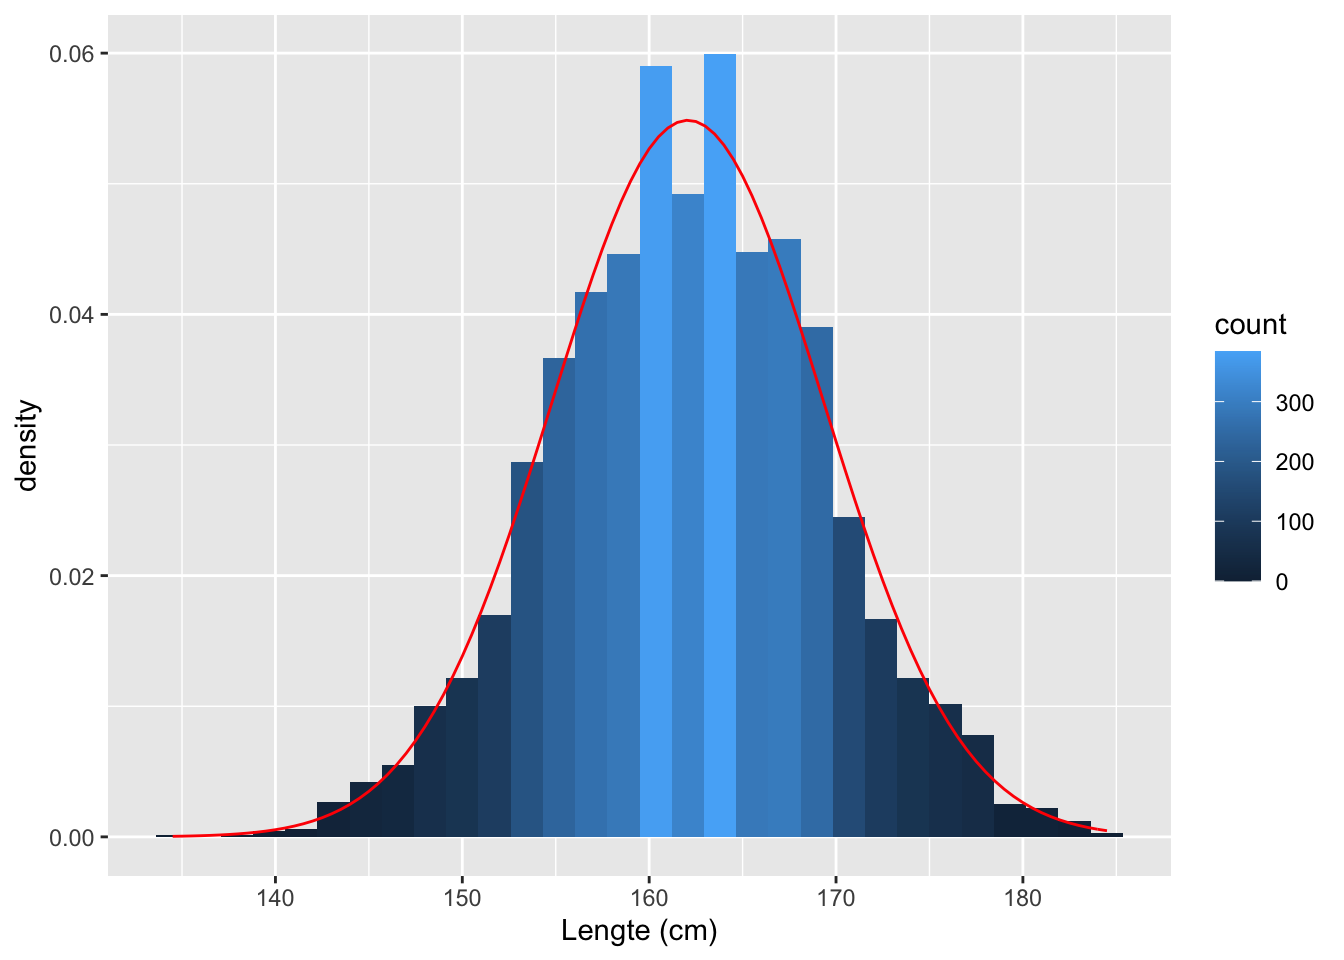
\includegraphics{Statistiek_2020_2021_files/figure-latex/unnamed-chunk-55-1.pdf}

We doen nu hetzelfde op basis van de steekproef met de 10 vrouwen.

\begin{Shaded}
\begin{Highlighting}[]
\NormalTok{HeightSum10 \textless{}{-}}\StringTok{ }\NormalTok{fem10 }\OperatorTok{\%\textgreater{}\%}\StringTok{ }\KeywordTok{summarize}\NormalTok{(}\DataTypeTok{mean =} \KeywordTok{mean}\NormalTok{(Height), }
    \DataTypeTok{sd =} \KeywordTok{sd}\NormalTok{(Height))}

\NormalTok{HeightSum10}
\end{Highlighting}
\end{Shaded}

\begin{verbatim}
## # A tibble: 1 x 2
##    mean    sd
##   <dbl> <dbl>
## 1  163.  8.19
\end{verbatim}

\begin{Shaded}
\begin{Highlighting}[]
\NormalTok{fem10 }\OperatorTok{\%\textgreater{}\%}\StringTok{ }\KeywordTok{ggplot}\NormalTok{(}\KeywordTok{aes}\NormalTok{(}\DataTypeTok{x =}\NormalTok{ Height)) }\OperatorTok{+}\StringTok{ }\KeywordTok{geom\_histogram}\NormalTok{(}\KeywordTok{aes}\NormalTok{(}\DataTypeTok{y =}\NormalTok{ ..density.., }
    \DataTypeTok{fill =}\NormalTok{ ..count..), }\DataTypeTok{bins =} \DecValTok{10}\NormalTok{) }\OperatorTok{+}\StringTok{ }\KeywordTok{xlab}\NormalTok{(}\StringTok{"Lengte (cm)"}\NormalTok{) }\OperatorTok{+}\StringTok{ }
\StringTok{    }\KeywordTok{stat\_function}\NormalTok{(}\DataTypeTok{fun =}\NormalTok{ dnorm, }\DataTypeTok{color =} \StringTok{"red"}\NormalTok{, }\DataTypeTok{args =} \KeywordTok{list}\NormalTok{(}\DataTypeTok{mean =}\NormalTok{ HeightSum10}\OperatorTok{$}\NormalTok{mean[}\DecValTok{1}\NormalTok{], }
        \DataTypeTok{sd =}\NormalTok{ HeightSum10}\OperatorTok{$}\NormalTok{sd[}\DecValTok{1}\NormalTok{])) }\OperatorTok{+}\StringTok{ }\KeywordTok{xlim}\NormalTok{(}\DecValTok{130}\NormalTok{, }\DecValTok{190}\NormalTok{)}
\end{Highlighting}
\end{Shaded}

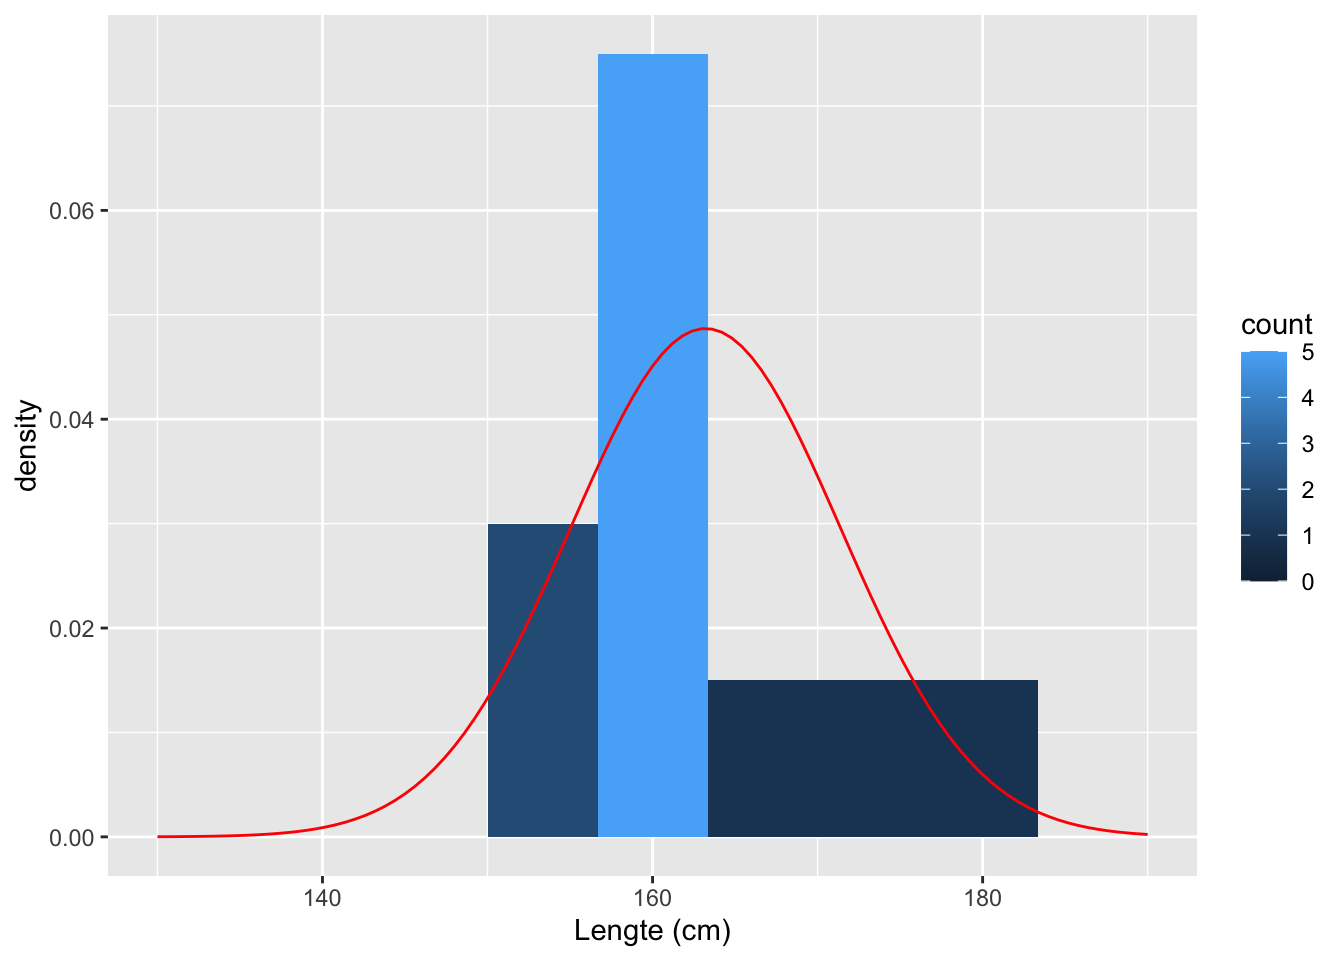
\includegraphics{Statistiek_2020_2021_files/figure-latex/unnamed-chunk-57-1.pdf}

We kunnen de normale benadering nu ook gebruiken om de kans te berekenen dat een vrouw kleiner is dan 150 cm: Pr(X \textless= 150).

We doen dit op basis van de volledige steekproef en vergelijken dit uit wat we bekomen met de ECDF.

\begin{Shaded}
\begin{Highlighting}[]
\KeywordTok{pnorm}\NormalTok{(}\DecValTok{150}\NormalTok{, HeightSum}\OperatorTok{$}\NormalTok{mean[}\DecValTok{1}\NormalTok{], HeightSum}\OperatorTok{$}\NormalTok{sd[}\DecValTok{1}\NormalTok{])}
\end{Highlighting}
\end{Shaded}

\begin{verbatim}
## [1] 0.0484516
\end{verbatim}

\begin{Shaded}
\begin{Highlighting}[]
\KeywordTok{ecdfFem}\NormalTok{(}\DecValTok{150}\NormalTok{)}
\end{Highlighting}
\end{Shaded}

\begin{verbatim}
## [1] 0.05222073
\end{verbatim}

Op basis van de kleine steekproef bekomen we:

\begin{Shaded}
\begin{Highlighting}[]
\KeywordTok{pnorm}\NormalTok{(}\DecValTok{150}\NormalTok{, HeightSum10}\OperatorTok{$}\NormalTok{mean[}\DecValTok{1}\NormalTok{], HeightSum10}\OperatorTok{$}\NormalTok{sd[}\DecValTok{1}\NormalTok{])}
\end{Highlighting}
\end{Shaded}

\begin{verbatim}
## [1] 0.05346615
\end{verbatim}

\begin{Shaded}
\begin{Highlighting}[]
\KeywordTok{ecdfFem10}\NormalTok{(}\DecValTok{150}\NormalTok{)}
\end{Highlighting}
\end{Shaded}

\begin{verbatim}
## [1] 0
\end{verbatim}

Voor kleine steekproef is geschatte kans o.b.v. empirische distributie veel minder nauwkeurig.
Kwantielen geschat o.b.v. kleine steekproef zijn immers vrij onzeker. Ze gebruiken immers maar een fractie van de data.\\
De schatting o.b.v. de normale verdeling laat toe om alle data te gebruiken voor het schatten van de model parameters en is daarom nauwkeuriger. Uiteraard heeft de laatste aanpak de beperking dat de data Normaal verdeeld moeten zijn.

\hypertarget{referentie-intervallen}{%
\subsection{Referentie intervallen}\label{referentie-intervallen}}

Het bepalen van grenswaarden voor de lengte die vrij veel voorkomen kunnen worden bekomen door gebruik te maken van een referentie interval.

Typisch wordt een 95\% referentie interval gebruikt zodat we voor 95\% van de subjecten in de populatie verwachten dat ze een karakteristiek hebben die in het referentie interval ligt.

We kunnen dat opnieuw op basis van de empirische distributie.

\begin{itemize}
\item
  We moeten hiervoor \(\hat{F}(x_{2.5\%})=0.025\) en \(\hat{F}(x_{97.5\%})=0.975\) berekenen zodat 95\% van de observaties in de steekproef vallen in het interval \([x_{2.5\%},x_{97.5\%}]\).
\item
  Dat kan met de \texttt{quantile} functie.
\end{itemize}

Grote steekproef

\begin{Shaded}
\begin{Highlighting}[]
\NormalTok{NHANES }\OperatorTok{\%\textgreater{}\%}\StringTok{ }\KeywordTok{filter}\NormalTok{(Gender }\OperatorTok{==}\StringTok{ "female"} \OperatorTok{\&}\StringTok{ }\OperatorTok{!}\KeywordTok{is.na}\NormalTok{(Height) }\OperatorTok{\&}\StringTok{ }
\StringTok{    }\NormalTok{Age }\OperatorTok{\textgreater{}}\StringTok{ }\DecValTok{18}\NormalTok{) }\OperatorTok{\%\textgreater{}\%}\StringTok{ }\KeywordTok{pull}\NormalTok{(Height) }\OperatorTok{\%\textgreater{}\%}\StringTok{ }\KeywordTok{quantile}\NormalTok{(}\DataTypeTok{prob =} \KeywordTok{c}\NormalTok{(}\FloatTok{0.025}\NormalTok{, }
    \FloatTok{0.975}\NormalTok{))}
\end{Highlighting}
\end{Shaded}

\begin{verbatim}
##  2.5% 97.5% 
## 147.6 176.7
\end{verbatim}

\begin{itemize}
\tightlist
\item
  Op basis van de grote steekproef schatten we dat 95\% van de vrouwen in de populatie een lengte heeft die ligt in het interval {[}147.6, 176.7{]}.
\end{itemize}

Kleine steekproef

\begin{Shaded}
\begin{Highlighting}[]
\NormalTok{fem10 }\OperatorTok{\%\textgreater{}\%}\StringTok{ }\KeywordTok{pull}\NormalTok{(Height) }\OperatorTok{\%\textgreater{}\%}\StringTok{ }\KeywordTok{quantile}\NormalTok{(}\DataTypeTok{prob =} \KeywordTok{c}\NormalTok{(}\FloatTok{0.025}\NormalTok{, }
    \FloatTok{0.975}\NormalTok{))}
\end{Highlighting}
\end{Shaded}

\begin{verbatim}
##     2.5%    97.5% 
## 154.7250 178.3275
\end{verbatim}

\begin{itemize}
\tightlist
\item
  Dit interval o.b.v. de kleine steekproef is een ruwe benadering.
\item
  We hebben immers niet voldoende observaties om een goede benadering te hebben voor extreme quantielen.
\end{itemize}

\hypertarget{normale-benadering-1}{%
\subsubsection{Normale benadering}\label{normale-benadering-1}}

We kunnen de functie qnorm gebruiken om quantielen te berekenen van de normale distributie. We weten dat een 95\% referentie interval ongeveer binnen twee standaard deviaties rond het gemiddelde ligt.

We doen dit nu voor de
- Grote steekproef

\begin{Shaded}
\begin{Highlighting}[]
\KeywordTok{qnorm}\NormalTok{(}\FloatTok{0.025}\NormalTok{, }\DataTypeTok{mean =}\NormalTok{ HeightSum}\OperatorTok{$}\NormalTok{mean, }\DataTypeTok{sd =}\NormalTok{ HeightSum}\OperatorTok{$}\NormalTok{sd)}
\end{Highlighting}
\end{Shaded}

\begin{verbatim}
## [1] 147.8192
\end{verbatim}

\begin{Shaded}
\begin{Highlighting}[]
\NormalTok{HeightSum}\OperatorTok{$}\NormalTok{mean }\OperatorTok{{-}}\StringTok{ }\DecValTok{2} \OperatorTok{*}\StringTok{ }\NormalTok{HeightSum}\OperatorTok{$}\NormalTok{sd}
\end{Highlighting}
\end{Shaded}

\begin{verbatim}
## [1] 147.528
\end{verbatim}

\begin{Shaded}
\begin{Highlighting}[]
\KeywordTok{qnorm}\NormalTok{(}\FloatTok{0.975}\NormalTok{, }\DataTypeTok{mean =}\NormalTok{ HeightSum}\OperatorTok{$}\NormalTok{mean, }\DataTypeTok{sd =}\NormalTok{ HeightSum}\OperatorTok{$}\NormalTok{sd)}
\end{Highlighting}
\end{Shaded}

\begin{verbatim}
## [1] 176.3237
\end{verbatim}

\begin{Shaded}
\begin{Highlighting}[]
\NormalTok{HeightSum}\OperatorTok{$}\NormalTok{mean }\OperatorTok{+}\StringTok{ }\DecValTok{2} \OperatorTok{*}\StringTok{ }\NormalTok{HeightSum}\OperatorTok{$}\NormalTok{sd}
\end{Highlighting}
\end{Shaded}

\begin{verbatim}
## [1] 176.6149
\end{verbatim}

\begin{itemize}
\tightlist
\item
  Kleine steekproef
\end{itemize}

\begin{Shaded}
\begin{Highlighting}[]
\KeywordTok{qnorm}\NormalTok{(}\FloatTok{0.025}\NormalTok{, }\DataTypeTok{mean =}\NormalTok{ HeightSum10}\OperatorTok{$}\NormalTok{mean, }\DataTypeTok{sd =}\NormalTok{ HeightSum10}\OperatorTok{$}\NormalTok{sd)}
\end{Highlighting}
\end{Shaded}

\begin{verbatim}
## [1] 147.1499
\end{verbatim}

\begin{Shaded}
\begin{Highlighting}[]
\KeywordTok{qnorm}\NormalTok{(}\FloatTok{0.975}\NormalTok{, }\DataTypeTok{mean =}\NormalTok{ HeightSum10}\OperatorTok{$}\NormalTok{mean, }\DataTypeTok{sd =}\NormalTok{ HeightSum10}\OperatorTok{$}\NormalTok{sd)}
\end{Highlighting}
\end{Shaded}

\begin{verbatim}
## [1] 179.2701
\end{verbatim}

We zien dat de benadering voor de kleine steekproef op basis van de aanname van Normaliteit opnieuw goed werkt!

\hypertarget{conclusions}{%
\subsection{Conclusions}\label{conclusions}}

\begin{itemize}
\item
  Voor de grote steekproef geven de empirische distributie en de normale benadering vergelijkbare resultaten.
\item
  Voor de kleine steekproef werkt de normale benadering beter dan de empirische distributie.

  \begin{itemize}
  \tightlist
  \item
    We kijken immers naar extreme quantielen 2.5\% en 97.5\%.
  \item
    Er zijn inderdaad weinig gegevens in de steekproef die toelaten om deze quantielen direct te schatten.
  \item
    Met de normale benadering kunnen we alle data gebruiken om het gemiddelde en de standaarddeviatie te schatten.
  \item
    Als de aanname van normaliteit geldt dan krijgen we betere schattingen voor deze kwantielen.
  \end{itemize}
\end{itemize}

\hypertarget{statistieken}{%
\section{Statistieken}\label{statistieken}}

Formules die gebruikt worden om parameters van de verdeling in de populatie te schatten op basis van de
steekproef, alsook het numerieke resultaat dat men bekomt door deze formules
te evalueren, worden \emph{statistieken} genoemd.
Bijvoorbeeld het
rekenkundig gemiddelde van alle systolische bloeddrukwaarden voor de verschillende subjecten
in de steekproef, is een statistiek. Statistieken zijn dus wat
de onderzoekers observeren of kunnen berekenen o.b.v. de gegevens in de
steekproef; parameters zijn wat ze eigenlijk willen weten.
Omdat statistieken berekend worden op basis van de gegevens uit de steekproef, zullen ze variëren van steekproef tot steekproef.
We zullen ze daarom noteren met een hoofdletter (bvb. \(\bar X\) voor het steekproefgemiddelde), tenzij we verwijzen naar de numerieke waarde die gerealiseerd wordt in een bepaalde steekproef, in welk geval we een kleine letter gebruiken (bvb. \(\bar x\) voor het steekproefgemiddelde).

\hypertarget{conventie}{%
\section{Conventie}\label{conventie}}

\textbf{Belangrijke Conventie:} In de cursus gebruiken we de conventie om \textbf{populatieparameters die een vaste waarden aannemen maar die meestal ongekend zijn} voor te stellen door \textbf{Griekse symbolen}. \textbf{Statistieken} waarmee we deze ongekende parameters schatten o.b.v. een steekproef zullen we weergeven door \textbf{letters}.

Voor de normaal verdeling hebben we dus:

\begin{longtable}[]{@{}cc@{}}
\toprule
Populatie & Steekproef\tabularnewline
\midrule
\endhead
\(\mu\) & \(\bar X\)\tabularnewline
\(\sigma^2\) & \(S^2\)\tabularnewline
\bottomrule
\end{longtable}

Om hetgeen we in de steekproef observeren te kunnen veralgemenen naar de populatie, zullen we gebruik moeten maken van methodes uit de statistische besluitvorming wat in latere hoofdstukken aan bod komt.

De cursus is als volgt georganiseerd:
In hoofdstuk \ref{chap:design} verdiepen we ons in studiedesign. Vervolgens gaan we in op data-exploratie in hoofdstuk \ref{chap:describe}, hierbij zullen we de gegevens in een steekproef grondig exploreren zodoende inzicht te verwerven in de data en hoe we ze statistisch kunnen modelleren.
In hoofdstuk \ref{chap:besluit} introduceren we de grondslagen van statistische besluitvorming die het ons mogelijk maakt om effecten die we observeren in de steekproef te kunnen veralgemenen naar de populatie toe.
In hoofdstukken \ref{chap:linReg}-\ref{chap:glm} zullen we meer geavanceerde statistische modellen en methoden introduceren om data te modelleren en voor statistische besluitvorming.

\hypertarget{code-voor-dit-hoofdstuk}{%
\section{Code voor dit hoofdstuk}\label{code-voor-dit-hoofdstuk}}

\begin{enumerate}
\def\labelenumi{\arabic{enumi}.}
\tightlist
\item
  Continue Toevallige Veranderlijken:
\end{enumerate}

\begin{enumerate}
\def\labelenumi{\arabic{enumi}.}
\setcounter{enumi}{1}
\tightlist
\item
  Lengte voorbeeld:
\end{enumerate}

\hypertarget{chap:design}{%
\chapter{Studiedesign}\label{chap:design}}

Alle kennisclips die in dit hoofdstuk zijn verwerkt kan je in deze youtube playlist vinden: \href{https://www.youtube.com/playlist?list=PLZH1hP8_LbJL1GjhnpEDlx78OJ6qUzSix}{Kennisclips Hoofdstuk3}

Link naar webpage/script die wordt gebruik in de kennisclips: \href{https://statomics.github.io/sbc20/rmd/03-experimentalDesign.html}{script Hoofdstuk3}

\hypertarget{inleiding-2}{%
\section{Inleiding}\label{inleiding-2}}

Centraal in wetenschappelijk onderzoek is de wens en noodzaak om
theorie-gebaseerde kennis empirisch (d.w.z. door middel van observatie) te
verifiëren en op te bouwen. Terwijl theorie-gebaseerde kennis voortvloeit uit hypothesen
omtrent het bestudeerde biologische of chemische proces, ontstaat empirische
kennis door lukraak subjecten (mensen, planten, dieren) uit een doelpopulatie te
trekken volgens een gestructureerd schema en hen vervolgens te observeren.
Dit gestructureerde schema, dat ondermeer vastlegt welke en hoeveel
subjecten in de studie worden opgenomen en eventueel wie welke experimentele
interventie zal ondergaan, noemt men het \emph{design} van de studie of de
\emph{proefopzet}. Met een goed design kunnen betrouwbare conclusies
worden getrokken op basis van de gegevens. Het bepaalt immers welke
informatie wel en niet in de dataset vervat zal zijn. Fouten bij het design
van een studie kunnen soms gecorrigeerd worden door de statistische analyse,
maar zijn helaas vaak onherroepelijk. Het design is daarom van cruciaal
belang voor een studie en vereist evenveel aandacht als de uiteindelijke
statistische analyse van de observaties. Ook in deze cursus vormen de
concepten in dit hoofdstuk rond design wellicht het meest
belangrijke onderwerp, hoewel we er slechts beknopt op in kunnen gaan. De
ideeën lijken eenvoudig, maar dat is vaak een bedrieglijke indruk!

\begin{figure}

{\centering 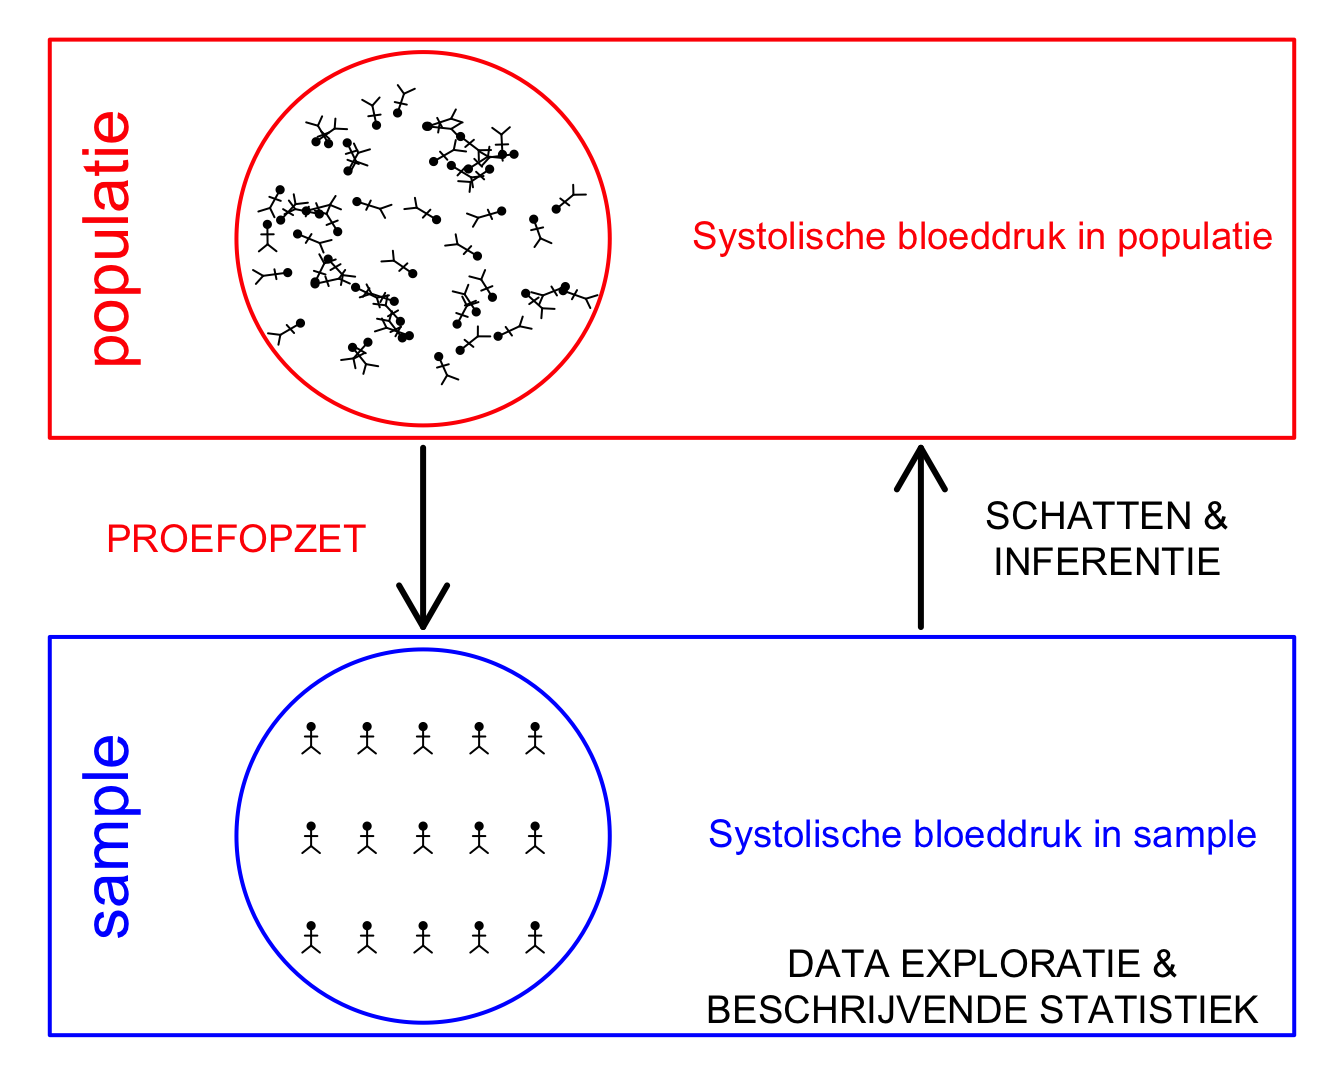
\includegraphics[width=1\linewidth]{Statistiek_2020_2021_files/figure-latex/pop2Samp2PopDesign-1} 

}

\caption{Verschillende stappen in een studie. In dit hoofdstuk ligt de focus op proefopzet.}\label{fig:pop2Samp2PopDesign}
\end{figure}

\hypertarget{sec:steekproefdesigns}{%
\section{Steekproefdesigns}\label{sec:steekproefdesigns}}

In de praktijk vestigt men de interesse van een onderzoek op een bepaalde biologische \emph{populatie}. Vervolgens zal men een geschikt type en grootte van monsters of stalen (of meer algemeen experimentele eenheden en/of subjecten genoemd doorheen deze cursus) definiëren waarvoor men metingen zal verzamelen. Bijvoorbeeld, indien men de grootte van de populatie salamanders van de species Plethodon jordani wenst te bestuderen, kan men de aandacht van het onderzoek vestigen op de bestaande populatie P. jordani in de Great Smoky Mountains (d.i. de populatie) en vervolgens het aantal salamanders tellen op oppervlakte-eenheden van 10 m\(^2\) (die eenheden zijn de stalen of ``experimentele eenheden''; voor elke experimentele eenheid bekomt men aldus een meting). Indien men de impact van roofvissen op zeebodemhabitats wenst te evalueren, dan kan het onderzoek de aandacht vestigen op de zeebodem binnen een afstand van 500 m voor de Belgische Noordzeekust (d.i. de biologische populatie) en kunnen vervolgens metingen worden verzameld op stukjes zeebodem met een straal van 1 m (d.i. de ``stalen'' in de studie). Omdat het in de praktijk bijna nooit mogelijk is om de hele populatie te onderzoeken (alle salamanders in de Great Smoky Mountains, de ganse zeebodem binnen een afstand van 500 m voor de Belgische Noordzeekust), zal men zich beperken tot gegevens voor een zogenaamde \emph{steekproef}, een beperkte verzameling stalen, experimentele eenheden of subjecten uit de populatie.

Welke subjecten uit de populatie men precies zal bestuderen, zal uiteraard zijn weerslag hebben op de resultaten van de uiteindelijke analyse van de gegevens. Opdat de resultaten die men observeert voor de steekproef veralgemeenbaar zouden zijn naar de ganse studiepopulatie, is het noodzakelijk dat men de subjecten uit de steekproef zodanig kiest dat ze representatief zijn voor de populatie. De basismethode om dat te realiseren, heet \emph{eenvoudige lukrake steekproeftrekking} (in het Engels: \emph{simple random sampling}). Ze bestaat erin te garanderen dat elk subject in de populatie een zelfde kans heeft om in de steekproef terecht te komen. Zo kan men bijvoorbeeld elke muis in een kooi een nummer geven en vervolgens lukraak een aantal \(n\) van die nummers trekken. In de praktijk, en in het bijzonder in de veldbiologie, is die methode echter vaak moeilijk toe te passen omdat de subjecten in de populatie bijvoorbeeld geen goed onderscheiden habitats vormen, niet op voorhand genummerd kunnen worden of omdat de populatie een te groot gebied bestrijkt. Zo is het bijvoorbeeld niet makkelijk om een eenvoudige lukrake steekproef van salamanders in de Great Smoky Mountains te bekomen omdat het bestudeerde gebied zeer groot is en de salamanders uiteraard niet genummerd kunnen worden. In die gevallen gaan biologen vaak over op \emph{haphazard sampling}, waarbij men op een minder formele manier stalen verzamelt, maar er toch voor probeert te zorgen dat de resultaten niet vertekend worden doordat bepaalde subjecten meer kans hebben om in de steekproef terecht te komen. Bijvoorbeeld kan men een computer lukraak plaatsen laten aanduiden in de Great Smoky Mountains en kan men vervolgens metingen proberen te verzamelen voor de eerste salamander die telkens in de buurt van de aangeduide plaatsen voorbijkomt.

Sommige steekproefdesigns houden expliciet rekening met heterogeniteit in de populatie waaruit een steekproef wordt genomen. Bij \emph{gestratificeerde lukrake steekproeven} (in het Engels: \emph{stratified random samples}) wordt de populatie opgedeeld in verschillende strata, die goed onderscheiden subgroepen in de populatie identificeren, en worden vervolgens eenvoudige lukrake steekproeven uit elk stratum genomen. Stel bijvoorbeeld dat men karakteristieken van stenen in een rivier wenst te beschrijven en dat stenen in verschillende habitats voorkomen (rotsige, ondiepe waters, diepe waters, stille binnenwaters,\ldots), dan kan het zinvol zijn om een gestratificeerde lukrake steekproef te nemen om ervoor te zorgen dat er binnen elk stratum (d.i. elke habitat) een voldoende aantal stenen verzameld worden.

Bij \emph{geclusterde steekproeftrekking} (in het Engels: \emph{cluster sampling}) worden clusters van meer verwante subjecten uit de populatie getrokken. Stel bijvoorbeeld dat we de impact van verschillende vormen van beschadiging aan bladeren van een boom wensen te meten, dan kunnen we in een eerste fase een eenvoudige lukrake steekproef van bomen bepalen. Vervolgens kunnen we in een tweede fase binnen elke boom een eenvoudige lukrake steekproef van bladeren bepalen en de verschillende gekozen bladeren aan verschillende vormen van beschadiging onderwerpen. Dit noemt men (two stage) cluster sampling omdat bladeren afkomstig van een zelfde boom meer verwant en bijgevolg geclusterd zijn. We zullen later zien dat men in de analyse van gegevens uit dergelijke studie met die clustering rekening moet houden.

Tenslotte steunt men in de biologische wetenschappen ook vaak op \emph{systematische steekproeven} waarbij men bijvoorbeeld monsters neemt die op vaste afstand van elkaar bekomen worden of op voorafgekozen tijdstippen, en om die reden niet volledig lukraak genoemd kunnen worden. Dit wordt vaak gebruikt wanneer men een omgevings- of tijdsgradiënt wenst te beschrijven voor een bepaald proces, zoals de wijziging in rijkdom aan species naarmate men zich verwijdert van een vervuilingsbron. Dergelijke designs zijn nuttig en logistiek zeer praktisch, maar kunnen vertekende resultaten opleveren wanneer de monsters op specifieke plaatsen genomen worden die samenvallen met een ongekende omgevings- of tijdsgradiënt (d.i. indien de gekozen plaatsen selectief zijn en afwijkend van de globale omgevings- of tijdsgradiënt).

\hypertarget{replicatie}{%
\subsection{Replicatie}\label{replicatie}}

Replicatie betekent dat herhaaldelijke observaties worden bekomen, op verschillende plaatsen, voor verschillende dieren of planten, op verschillende tijdstippen, \ldots{} Dergelijke herhalingen zijn essentieel in empirisch onderzoek omdat biologische en ecologische systemen vaak zeer variabel zijn en de beschikbaarheid van meerdere observaties toelaat om ruis op de gegevens te drukken. Hoewel biologen, biotechnologen en biochemici zich goed bewust zijn van de nood voor replicatie wordt vaak misbegrepen op welke schaal die herhalingen moeten bekomen worden. Wellicht is er geen enkel aspect van studiedesign dat meer verwarring veroorzaakt bij wetenschappers dan dit. Stel bijvoorbeeld dat men een studie wenst op te zetten om het effect van bosbranden op de rijkdom aan ongewervelde dieren te onderzoeken. Meestal zal men dan gebruik maken van natuurlijke bosbranden. Stel dat 1 verbrand gebied gelocaliseerd wordt en vergeleken wordt met een naburig gebied waar geen bosbrand plaatsvond. Stel verder dat men binnen elk gebied verschillende stalen bodemkorst neemt om de rijkdom aan ongewervelden te bepalen. Dan beschikt men wel over herhaaldelijke metingen (namelijk verschillende stukken bodemkorst per gebied), maar niet op de juiste schaal. De metingen voor de rijkdom aan species die men uit het verbrande gebied bekomen heeft, meten immers de impact van dezelfde brand. Als gevolg daarvan kan men op basis van eventuele verschillen in species rijkdom tussen beide gebieden niet bepalen of ze het gevolg zijn van de brand dan wel van andere verschillen tussen beide gebieden die eveneens een impact op ongewervelden hebben. Uit dergelijke vergelijking kan men hoogstens besluiten dat de gebieden al dan niet verschillen, maar niet waardoor ze verschillen.

De herhaalde stukken bodemkorst in bovenstaand voorbeeld stellen substeekproeven voor. Deze stellen geen herhalingen voor van de bestudeerde interventie (bosbranden) en worden daarom pseudoreplicaties genoemd. Pseudoreplicaties zijn nuttig omdat ze replicaties zijn (op een zeker niveau) en daardoor toelaten om een deel van de ruis op de gegevens weg te middelen. In sommige studies zijn echte replicaties onmogelijk en is het bijgevolg onvermijdelijk om zijn toevlucht tot pseudoreplicaties te nemen. Bijvoorbeeld, indien men een experiment uitvoert dat kamers van constante temperatuur vereist, dan kan het best zijn dat er binnen een gegeven instituut slechts een tweetal dergelijke kamers beschikbaar zijn omwille van hun hoge kost. Indien men bijvoorbeeld de impact wenst te onderzoeken van rioollozing op de biomassa van phytoplankton in een bepaalde kuststreek, dan is er vaak maar 1 riool waarin men echt geïnteresseerd is, terwijl het aantal naburige lokaties zonder riool zeer uitgebreid kan zijn. In dat geval zal men vaak stalen nemen op meerdere plaatsen zonder riool om in ieder geval de variatie tussen controlesites (d.i. sites zonder rioollozing) te minimaliseren. \emph{Before-After-Control-Impact (BACI) designs} proberen verder informatie te winnen door zowel metingen te nemen vóór de interventie (bvb. het plaatsen van een riool) als na de interventie.

\hypertarget{experimentele-studies}{%
\section{Experimentele studies}\label{experimentele-studies}}

Studiedesigns worden opgesplits in \emph{experimentele studies of experimenten} waar de onderzoeker eerst het biologische systeem manipuleert en vervolgens observeert, en \emph{observationele studies} waar de onderzoeker enkel observeert zonder zelf in het systeem in te grijpen. In deze sectie gaan we dieper in op het eerste type studies. Observationele studies worden besproken in Sectie \ref{sec:observational}.

\begin{definition}[experiment]
\protect\hypertarget{def:unnamed-chunk-64}{}{\label{def:unnamed-chunk-64} \iffalse (experiment) \fi{} }
\end{definition}
Een \textbf{experiment} is een reeks observaties die gemaakt worden onder
condities die gecontroleerd worden door de onderzoeker. De onderzoeker
controleert hierbij verschillende factoren (zoals de keuze van de
interventie voor een locatie, plant, dier), met als doel een zuiver antwoord op de gestelde onderzoeksvraag te bepalen.
\footnote{Met ``zuiver'' wordt hier bedoeld dat de het zuivere interventie-effect uit de gegevens
  kan gehaald worden zonder dat het antwoord wordt beïnvloed door andere aspecten/variabelen. Dit wordt meer concreet in Hoofdstuk \{chap:sample\}
  uitgelegd. Voorlopig volstaat de intuïtieve betekenis van het woord.}

\textbf{Einde definitie}

Bijvoorbeeld, wanneer een dierenfysioloog 2 behandelingen wenst te vergelijken tussen experimentele dieren,
dan kan hij - zoals we in dit hoofdstuk zullen zien - vermijden dat het
behandelingseffect vertekend\footnote{ Voorlopig verstaan we onder het feit dat een schatting voor het
  behandelingseffect `vertekend' is, dat het foutief werd ingeschat of, m.a.w., dat het geschatte effect niet correct het zuivere effect van de behandeling weerspiegelt. Een meer concrete definitie volgt eveneens in
  Hoofdstuk \{chap:sample\}.} is door vergelijkbare groepen dieren te creëren;
bijvoorbeeld, door lukraak (bijvoorbeeld door
het opgooien van een muntstuk) te bepalen welke behandeling aan welk
dier wordt toegediend.

\hypertarget{de-salk-vaccin-veldstudie}{%
\subsection{De Salk Vaccin Veldstudie}\label{de-salk-vaccin-veldstudie}}

Om de basisprincipes van experimentele designs in te voeren, gebruiken we als rode draad de Salk Vaccin Veldstudie. Vooraleer dieper op deze studie in te gaan, schetsen we de historische context.

De eerste polio-epidemie in de Verenigde Staten brak uit in 1916 en kostte
aan honderdduizenden mensen, vooral kinderen, het leven. Tegen de jaren 1950
waren er verschillende vaccins ontwikkeld. Vooral het vaccin dat door John
Salk werd ontwikkeld, leek veelbelovend omdat het zich veilig en effectief
had getoond in laboratoriumstudies. In 1954 werd door de National Foundation
for Infantile Paralysis (NFIP) een grote studie opgezet om de effectiviteit
van het vaccin buiten het laboratorium na te gaan. Meer concreet wenstte men
na te gaan wat de invloed was van vaccinatie op de polio-incidentie.

\begin{definition}[incidentie en prevalentie]
\protect\hypertarget{def:unnamed-chunk-65}{}{\label{def:unnamed-chunk-65} \iffalse (incidentie en prevalentie) \fi{} }
\end{definition}
De \textbf{incidentie} van een bepaalde ziekte of aandoening (bvb. polio)
wordt gedefinieerd als het verwachte aantal nieuwe gevallen van die ziekte
dat optreedt gedurende een vooraf bepaald tijdsinterval, uitgedrukt per
eenheid van een ziektevrije populatie. Het drukt m.a.w. de kans uit dat een
individu zonder de bestudeerde aandoening tijdens het gegeven tijdsinterval
deze aandoening zal opdoen.

De \textbf{prevalentie} van een bepaalde ziekte wordt gedefinieerd als de
proportie individuen met de ziekte in een bepaalde populatie op een bepaald
punt in de tijd.

\textbf{Einde definitie}

Stel dat de NFIP het vaccin gewoon had toegediend aan een groot aantal
kinderen en dat ze een daling observeerden in de incidentie van polio van
1953 naar 1954. Dit betekent dat de kans dat een lukraak polio-vrij kind een
polio-infectie opdeed in de loop van 1954 (d.i. de incidentie van polio in
1954), lager is dan de kans dat lukraak polio-vrij kind een polio-infectie
opdoet in de loop van 1953 (d.i. de incidentie van polio in 1953). In dat
geval kan men niet zomaar besluiten dat het vaccin effectief is. Immers,
afgezien van de introductie van een vaccin, varieert de incidentie van polio
van jaar tot jaar. Zo zou men, indien het vaccin niet effectief was, toch
een daling in polio-incidentie van 1953 naar 1954 kunnen vaststellen in
geval 1954 geen epidemisch jaar zou zijn.

De enige manier om te ontdekken of het vaccin effectief is, is om \emph{gelijktijdig} de incidentie van polio in 1954 te vergelijken tussen een
groep gevaccineerde kinderen (doorgaans \emph{cases} genoemd) en een groep
niet-gevaccineerde kinderen (doorgaans \emph{controles} genoemd). Dit is
wat de NFIP heeft gedaan. De deelnemers aan de studie waren kinderen uit de
leeftijdsgroepen die het meest vatbaar waren voor polio. De studie verliep in
verschillende schooldistricten in de Verenigde Staten waar het risico op
polio hoog was. Aan ongeveer 350000 kinderen uit de tweede graad werd
vaccinatie voorgeschreven. Voor 125000 van hen weigerden de ouders
toestemming te geven om deze vaccinatie te laten doorgaan, zodat de groep
cases uiteindelijk uit de overige 225000 kinderen bestond. Ongeveer
750000 kinderen uit de eerste en derde graad werden vrijwillig niet
gevaccineerd; zij vormden de controles.

Het feit dat de groep cases en de groep controles een verschillende grootte
hebben is niet problematisch zolang men niet het absolute aantal, maar het
percentage polio-besmettingen tussen beide groepen vergelijkt. Toch hoeft
een geobserveerd verschil in incidentie tussen gevaccineerde en
niet-gevaccineerde kinderen nog steeds niet noodzakelijk te impliceren dat
het vaccin effectief is. Hier zijn verschillende redenen voor:

\begin{enumerate}
\def\labelenumi{\arabic{enumi}.}
\tightlist
\item
  Ten eerste zou het kunnen dat men door toeval een verschil in
  incidentie waarneemt tussen beide groepen, doordat er per toeval
  bijvoorbeeld relatief gezien minder kinderen in de gevaccineerde groep polio
  ontwikkelen. In Hoofdstuk \ref{chap:besluit} zullen we methoden aanleren om
  uit te maken of een geobserveerd vaccinatie-effect (d.w.z. een
  vaccinatie-effect dat geschat of berekend werd o.b.v. de gegevens) al dan
  niet toevallig is.
\item
  Ten tweede zou het kunnen dat kinderen uit de tweede graad sowieso
  meer vatbaar zijn voor polio en er, afgezien van het werkelijke
  vaccin-effect, voor de cases dus een hogere incidentie wordt verwacht.
\item
  Ten derde is het zo dat vooral ouders uit hoge-inkomens gezinnen
  geneigd waren om de toestemming te geven hun kind te laten vaccineren, zodat
  de groep cases hoofdzakelijk bestaat uit kinderen van hoge-inkomens
  gezinnen. Deze kinderen zijn meer vatbaar voor polio omdat ze, wegens de
  betere hygiënische omstandigheden in deze gezinnen, minder antilichamen
  tegen polio ontwikkeld hebben.
\end{enumerate}

Het geobserveerde verschil in incidentie tussen gevaccineerde en
niet-gevaccineerde kinderen weerspiegelt daarom niet alleen de effectiviteit
van het vaccin, maar ook het feit dat kinderen uit graad 2 mogelijks niet
vergelijkbaar zijn met de resterende kinderen en het feit dat cases, omwille
van betere hygiënische omstandigheden, meer vatbaar zijn voor polio dan
controles. In het bijzonder is het om die reden mogelijk om, zelfs als het
vaccin effectief is, een gelijke incidentie voor cases en controles vast te
stellen. In dat geval verwart men het effect van het vaccin met het feit dat
cases meer vatbaar zijn voor polio dan controles.

De statistische les die we hier algemeen uit kunnen trekken, is dat de
verschillende interventiegroepen zo vergelijkbaar mogelijk moeten zijn bij
de bepaling van het effect van een interventie, opdat elk verschil in respons tussen
de groepen volledig kan toegeschreven worden aan de verschillende
interventie. Wanneer de groepen cases en controles niet volledig
vergelijkbaar zijn in een bepaalde factor (zoals de vatbaarheid voor polio,
maar niet de interventie zelf), dan is het mogelijk dat het effect van die
factor verward (in het Engels: \emph{confounded}) wordt met het effect van
de interventie. Men noemt die factor dan een confounder voor het effect van
de interventie. De belangrijkste beperking op de ondubbelzinnige interpretatie van studieresultaten is het probleem van confounding.

\begin{example}[De nood aan controle]
\protect\hypertarget{exm:unnamed-chunk-66}{}{\label{exm:unnamed-chunk-66} \iffalse (De nood aan controle) \fi{} }
\end{example}
Hairston (1980) bestudeerde de stelling dat 2 soorten salamander (P. jordani en P. glutinosus) in de Great Smoky Mountains mekaar rivaliseren. Hij zette daartoe experimenten op waarbij P. glutinosus verwijderd werd van bepaalde territoria. De populatie van P. jordani begon toe te nemen in de 3 jaren die volgden op de verwijdering van de salamanders, maar nam al even sterk toe op controleterritoria waar P. glutinosus niet verwijderd was. Had Hairston geen controleterritoria onderzocht, dan had hij mogelijks de toename in de populatie van P. jordani verkeerdelijk toegeschreven aan het verwijderen van P. glutinosus.

\textbf{Einde voorbeeld}

\begin{definition}[confounding en confounder]
\protect\hypertarget{def:unnamed-chunk-67}{}{\label{def:unnamed-chunk-67} \iffalse (confounding en confounder) \fi{} }
\end{definition}
\textbf{Confounding} is het probleem dat verschillen ten gevolge van verschillende experimentele interventies niet kunnen losgekoppeld worden van andere factoren, \textbf{confounders} genoemd, die verschillen tussen de interventiegroepen. Een confounder manifesteert zich als een variabele die geassocieerd
is met de blootstelling of interventie (bvb. gevaccineerd of niet) en de uitkomst (bvb.
polio-geïnfecteerd of niet), maar die door geen van beiden zelf beïnvloed wordt. Bijvoorbeeld, vatbaarheid voor polio is geassocieerd met de
keuze van de ouders om hun kind te laten vaccineren (d.i. de blootstelling)
alsook met de infectiestatus van het kind (d.i. de uitkomst), maar wordt
door geen van beiden zelf veroorzaakt. Confounders verstoren de associatie
tussen blootstelling en uitkomst zodat de geobserveerde associatie tussen
beiden mogelijks niet het pure effect (d.i. het causale effect) van die
blootstelling op die uitkomst uitdrukt.

\textbf{Einde definitie}

\begin{example}[Confounding in mariene veldexperimenten]
\protect\hypertarget{exm:unnamed-chunk-68}{}{\label{exm:unnamed-chunk-68} \iffalse (Confounding in mariene veldexperimenten) \fi{} }
\end{example}
Om het effect te onderzoeken van roofvissen op mariene zeebodemhabitats zou men gebieden met en zonder viskooien kunnen vergelijken. Als men vervolgens verschillen observeert tussen beide types gebieden, dan kan dat het gevolg zijn van het verwijderen van roofvissen (via de kooien), maar eveneens van de aanwezigheid van kooien (bijvoorbeeld, door schaduw die de kooi afwerpt, door de afgenomen waterstroming, \ldots). Het effect van roofvissen verwijderen wordt dus mogelijks verward met het effect van kooien plaatsen. De aanwezigheid van kooien manifesteert zich hier dus als een confounder. Om dergelijke confounding te vermijden, kan men controlekooien met grote gaten plaatsen waar de vis vrij in en uit kan zwemmen, maar die voor de rest vergelijkbaar zijn met de experimentele kooien. In dat geval zijn beide studiegebieden van kooien voorzien en zal een vergelijking van experimentele en controlekooien duidelijk een veel meer betrouwbare evaluatie toelaten van het effect van roofvissen. Toch blijft dergelijke vergelijking niet gegarandeerd vrij van confounding. Bijvoorbeeld, als het effect van kooien plaatsen er voornamelijk in bestaat om de stroming van water (en bijgevolg sedimentatie) te beïnvloeden, dan speelt de vraag of de stroming van water ook niet beïnvloed wordt door het feit dat vissen, omwille van de grote gaten, makkelijker in controlekooien zwemmen dan in experimentele kooien.

\textbf{Einde voorbeeld}

Heel wat experten in volksgezondheid zagen de problemen met het NFIP design
en suggereerden dat de controles uit dezelfde populatie moesten gekozen
worden als de cases (d.w.z. dat ze moesten vergelijkbaar zijn).
Vergelijkbaarheid van beide groepen garanderen, zou kunnen gebeuren op basis
van menselijk oordeel. Ervaring heeft niettemin aangetoond dat dit vaak niet
succesvol is omdat het zich makkelijk leent tot het bewust of onbewust
bevoordelen van de ene groep versus de andere. Het is daarom aangewezen om
\emph{randomisatieprocedures} toe te passen, waarbij de toewijzing van
mensen aan verschillende interventie-armen volledig lukraak gebeurt. Men
zegt in dat geval dat de studie \emph{gerandomiseerd gecontroleerd}(in
het Engels: \emph{randomized controlled}) is.

\begin{definition}[gerandomiseerde studie]
\protect\hypertarget{def:unnamed-chunk-69}{}{\label{def:unnamed-chunk-69} \iffalse (gerandomiseerde studie) \fi{} }
\end{definition}
Een \textbf{gerandomiseerd gecontroleerde} studie is een experiment waarbij
de toewijzing van subjecten aan de verschillende interventie-armen volledig
lukraak gebeurt zodat de toewijzing van een gegeven subject onmogelijk op
voorhand voorspeld kan worden. Als gevolg hiervan zijn de verschillende
interventiegroepen (in principe\footnote{We beklemtonen dat dit \emph{in principe} zo is, omdat er binnen een beperkt experiment (d.w.z met een relatief klein aantal proefpersonen/proefdieren) uiteraard toevallige verschillen tussen beide groepen kunnen ontstaan; we komen hier later op terug.}) in alle gekende en ongekende factoren (zoals
leeftijd, lichaamsgewicht, vatbaarheid voor polio \ldots) vergelijkbaar zodat
geobserveerde verschillen in uitkomst tussen de verschillende groepen (in
principe) kunnen toegeschreven worden aan de interventie (d.i. het vaccin).

\textbf{Einde definitie}

Naast de NFIP studie werd voor het Salk vaccin een gerandomiseerd
gecontroleerde studie opgezet waarbij de beslissing om aan een gegeven kind
al dan niet het vaccin toe te dienen, gemaakt werd door het opgooien van een
muntstuk. De \emph{randomisatie} werd uitgevoerd onder kinderen die van
hun ouders de toestemming kregen om zich te laten vaccineren, indien ze aan de
vaccin-groep zouden toegewezen worden. Door de randomisatie pas uit te
voeren na het krijgen van de toestemming tot vaccinatie, kon men vermijden
dat er \emph{differentiële uitval} was van kinderen in beide
groepen. Met differentiële uitval wordt bedoeld dat de reden om niet
deel te nemen aan de studie verschillend is voor de test-en controlegroep.
Dit kan vooral voorkomen in klinische studies (d.i. experimenten bij mensen)
wanneer 1 van beide behandelingen (in de test- of
controle-arm) een zware heelkundige ingreep is die vooral door ernstig zieke
mensen gemeden wordt. Wanneer er na randomisatie differentiële uitval
optreedt, dan kan men niet langer vergelijkbare groepen garanderen.

In de gerandomiseerde Salk vaccin studie werd aan kinderen in de
controle-groep een \emph{placebo} toegediend. Dat is een inerte, inactieve
behandeling; in dit geval een injectie van zout opgelost in water. Tijdens
de studie waren de kinderen \emph{blind} voor de behandelingscode (d.i. ze
wisten niet aan welke interventiegroep ze toegewezen waren). Dit heeft tot
gevolg dat hun respons op de vaccinatie (d.i. of ze al dan niet polio
ontwikkelen) het gevolg was van het al dan niet krijgen van het vaccin, en
niet van het `idee' om al dan niet behandeld te zijn. In deze studie lijkt het misschien onwaarschijnlijk dat het idee
om gevaccineerd te zijn de kinderen zou kunnen beschermen tegen polio, maar
de rol van het onderbewustzijn is soms sterker dan vermoed wordt. Zo heeft
men in een studie van patiënten met ernstige post-operatieve pijn
vastgesteld dat de pijn bij een derde van de patiënten spontaan verdween
na inname van een volledig neutrale substantie!

Het blinderen van de toegediende interventie laat algemeen toe om een zo objectief mogelijk
beeld van het interventie-effect te verkrijgen. Analoog gebruiken fysiologen in dierenexperimenten injectie met een zoutoplossing als controle i.p.v. geen injectie. Op die manier vermijden ze dat verschillen die men observeert tussen controledieren en dieren die een toxische substantie ingespoten krijgen, niet het gevolg zijn van de injectieprocedure (bijvoorbeeld, van wondjes ten gevolge van de inspuiting), maar van de ingespoten substantie zelf.

Een verdere voorzorgsmaatregel in de Salk vaccin studie was dat ook de
dokters, die moesten vaststellen of de kinderen geïnfecteerd waren,
blind waren voor de behandeling. Op die manier voorkwam men dat de arts
bewust of onbewust kennis omtrent de gekregen vaccinatie zou gebruiken om
een beslissing te nemen over de infectiestatus. Dit zou kunnen voorvallen
wanneer het resultaat van de polio-test dubieus was en de arts (bewust of
onbewust) kennis omtrent de vaccinatie-status van zijn patiënt gebruikt om
de infectie-status te bepalen. Om dezelfde reden zijn ook dierenfysiologen idealiter blind voor de substantie die bij elke rat ingespoten werd.

Omdat noch de arts, noch de patiënt in de Salk vaccin studie wisten welke
behandeling werd toegediend, wordt deze studie \emph{dubbel blind}
genoemd. Dubbel blinde studies vereisen dat de verschillende interventies er
hetzelfde uitzien.

\begin{table}

\caption{\label{tab:nfipStudy}De NFIP studie: aantal kinderen en incidentie (uitgedrukt per
100000 kinderen per jaar).}
\centering
\begin{tabular}[t]{lrr}
\toprule
  & Aantal & Incidentie\\
\midrule
Vaccin & 225000 & 25\\
Controle & 725000 & 54\\
Geen toestemming & 125000 & 44\\
\bottomrule
\end{tabular}
\end{table}

Tabellen \ref{tab:nfipStudy} en \ref{tab:dbrcStudy} geven de resultaten weer die geobserveerd
werden in de NFIP studie en het \emph{dubbel blinde gerandomiseerd
gecontroleerde} (in het Engels: \emph{double blind randomized controlled})
experiment. Op basis van Tabel \ref{tab:dbrcStudy} stellen we vast dat de incidentie
daalt van 71 tot 28 gevallen per 100000 per jaar als gevolg van
toediening van het vaccin. De enige vraag die resteert is of dergelijk
verschil in incidentie gewoon door toeval kan ontstaan wanneer in
werkelijkheid het vaccin geen effect zou hebben. Een gevorderde statistische analyse heeft aangetoond dat het bijna onmogelijk is om dergelijk verschil in incidentie
te observeren door toeval, wanneer het vaccin geen effect heeft. We mogen
dus besluiten dat het Salk vaccin effectief is.

Merk tenslotte op dat er inderdaad confounding optreedt in de NFIP studie. Immers
de polio-incidentie lijkt er veel minder te dalen dan in de gerandomiseerde studie, namelijk van 54 naar 25
per 100000 per jaar als gevolg van het vaccin (zie Tabel \ref{tab:nfipStudy}). De oorzaak is dat
de controlegroep in deze studie kinderen bevat die minder vatbaar zijn voor
polio dan de vaccin-groep.

\begin{table}

\caption{\label{tab:dbrcStudy}De gerandomiseerd gecontroleerde studie: aantal kinderen en incidentie (uitgedrukt per
100000 kinderen per jaar).}
\centering
\begin{tabular}[t]{lrr}
\toprule
  & Aantal & Incidentie\\
\midrule
Vaccin & 200000 & 28\\
Controle & 200000 & 71\\
Geen toestemming & 350000 & 46\\
\bottomrule
\end{tabular}
\end{table}

\hypertarget{gerandomiseerde-gecontroleerde-studies}{%
\subsection{Gerandomiseerde gecontroleerde studies}\label{gerandomiseerde-gecontroleerde-studies}}

Bij randomisatie heeft elk subject in de studie (bijvoorbeeld, elk kind in de Salk vaccin studie, elke studieplaats op de zeebodem waar men een kooi wil plaatsen) een gekende kans om elke interventie te krijgen (bvb. bij het opgooien van een muntje heeft men 50\% kans om het
vaccin te krijgen en 50\% kans om het placebo te krijgen), maar de te
ontvangen behandeling kan niet voorspeld worden. Vreemd genoeg wordt de nood
aan randomisatie niet steeds ingezien en maakt men vaak verkeerdelijk geen
onderscheid met \emph{systematische allocatie}.

\begin{definition}[systematische allocatie]
\protect\hypertarget{def:unnamed-chunk-70}{}{\label{def:unnamed-chunk-70} \iffalse (systematische allocatie) \fi{} }
\end{definition}
\textbf{Systematische allocatie} of \textbf{louter toevallige allocatie}
\emph{(in het Engels: haphazard allocation)} is een toewijzingsmethode die
mogelijks op een lukraak mechanisme lijkt, maar waarbij men de toewijzing
van (sommige) subjecten op voorhand kan voorspellen.

\textbf{Einde definitie}

Een typisch voorbeeld van een systematische toewijzingsmethode is er één
waarbij subjecten afgewisseld toegewezen worden aan de controle- of
interventiegroep. Het feit dat men hier de toewijzing van elk subject op voorhand kan
voorspellen, kan tot gevolg hebben dat de onderzoeker de toewijzing
manipuleert. In medisch onderzoek is het in het verleden zo meermaals gebeurd dat artsen de al te zieke patiënten die in principe aan de
controle arm zouden moeten toegewezen worden, later op bezoek laten komen
(zodat ze de testbehandeling krijgen) of niet in de studie opnemen. Dit
kan er op zijn beurt voor zorgen dat de verschillende groepen niet langer
vergelijkbaar zijn. Om systematische allocatie te vermijden, is het van
belang om een degelijke randomisatietechniek toe te passen. In de volgende
paragrafen geven we een aantal mogelijkheden hiertoe.

Bij \emph{eenvoudige randomisatie} worden subjecten lukraak toegewezen
aan interventie A of B door het opgooien van een muntje, dobbelsteen, \ldots{}
Vaak is het efficiënter om via de computer een randomisatielijst te
genereren die het proces van het opgooien van een muntje nabootst. Dit
vermijdt tevens de mogelijkheid dat de onderzoeker niet naar behoren zou
randomiseren (door bvb. het muntje zolang op te gooien tot de gewenste
interventiecode te zien is).

Hoewel eenvoudige randomisatie aan iedereen evenveel kans geeft om
behandeling A of B te krijgen, verzekert het niet dat beide groepen
uiteindelijk even groot zullen zijn. Zelfs in relatief grote studies kan
door toeval het verschil in aantal deelnemers in elke groep relatief groot
zijn. Men kan aantonen dat, als gevolg hiervan, het interventie-effect
doorgaans minder nauwkeurig of minder precies geschat kan worden op basis
van de gegevens dan wanneer beide groepen even groot zouden zijn. Daarmee
wordt bedoeld dat wanneer men de studie meermaals zou uitvoeren onder
identieke omstandigheden, de resultaten doorgaans meer variabel zullen zijn
van studie tot studie wanneer de relatieve grootte van beide groepen onbeperkt
is, dan wanneer men telkens groepen van gelijke grootte eist.

Om na randomisatie 2 behandelingsarmen van gelijke grootte te bekomen, kan
\emph{gebalanceerde} of \emph{beperkte randomisatie} (in het Engels:
\emph{balanced} of \emph{restricted randomisation}) worden gebruikt.
Hierbij wordt de randomisatieprocedure zó georganiseerd dat gelijke
aantallen subjecten worden toegewezen aan interventie A of B per blok van
bijvoorbeeld 4 subjecten. Eén methode om dat te doen is om enkel
sequenties te beschouwen van de vorm (1) AABB, (2) ABAB, (3) ABBA, (4) BABA,
(5) BAAB, (6) BBAA. Met behulp van een dobbelsteen of randomisatielijst
wordt lukraak een nummer van 1 tot 6 gekozen. Stel dat het 1 is. Dan worden
de 2 eerstvolgende subjecten toegewezen aan A en de 2 daarna aan B.
Vervolgens wordt een nieuw lukraak nummer tussen 1 en 6 getrokken,
enzovoort\ldots{}

Gebalanceerde randomisatie met blokken van grootte 1 is equivalent aan
eenvoudige randomisatie. Dergelijke blokgrootte is dus niet opportuun
wanneer men groepen van gelijke grootte wenst te bekomen.
Doorgaans is het niettemin zinvol om relatief kleine blokgroottes te
beschouwen. Bovenstaande procedure garandeert immers dat, wanneer de studie
halfweg een blok eindigt, het verschil in aantal subjecten tussen beide
groepen hoogstens de helft van de gekozen blokgrootte bedraagt.
Kleine blokken garanderen bijgevolg kleine verschillen in aantallen deelnemers per groep.

Bij een echte randomisatie hoeven de blokken niet allen dezelfde grootte te
hebben. Door de lengte van elk blok te variëren (bijvoorbeeld door een
lukraak mechanisme) verloopt de reeks toewijzingen van subjecten aan
interventie meer lukraak en voorkomt men dat de onderzoeker de blokgrootte ontdekt
en als gevolg daarvan de interventiecode van sommige subjecten kan
voorspellen. Immers, indien de onderzoeker de blokgrootte kent, dan kan hij net vóór het verstrijken van elk blok voorspellen wat de interventiecode
is van het laatste subject. Gebalanceerde randomisatie voor blokken
van verschillende grootte is niet veel moeilijker dan voor blokken van
gelijke grootte. Voor het vergelijken van 2 interventies zou men
bijvoorbeeld telkens eerst lukraak kunnen kiezen uit een blokgrootte van 2,
4 of 6 en vervolgens, zoals voorheen, lukraak een blok van die grootte
kiezen.

\begin{example}[Confounding in mariene veldexperimenten, vervolg]
\protect\hypertarget{exm:unnamed-chunk-71}{}{\label{exm:unnamed-chunk-71} \iffalse (Confounding in mariene veldexperimenten, vervolg) \fi{} }
\end{example}
Beschouw opnieuw het experiment naar het effect van roofvissen op zeebodemhabitats. Stel dat we 12 lukrake gebieden op de zeebodem gemarkeerd hebben en vervolgens wensen te beslissen waar we de experimentele kooien (die effectief vis vasthouden) en de controlekooien zullen plaatsen. Dan zouden we de kooien kunnen randomiseren door op elke plaats een muntje op te gooien en vervolgens een experimentele kooi te plaatsen wanneer men kop gooit en een controlekooi anders. Die procedure is erop gericht te garanderen dat experimentele kooien op vergelijkbare plaatsen opgesteld worden als controlekooien. Om te vermijden dat er, per toeval, meer controlekooien dan experimentele kooien geplaatst worden, kunnen we een gebalanceerde randomisatie uitvoeren met blokken van grootte 2. Hoe men dit kan uitvoeren, ligt echter minder voor de hand. Eén mogelijkheid kan erin bestaan om de verschillende gebieden willekeurig te nummeren en die nummers lukraak dooreen te gooien teneinde een nieuwe nummering te bekomen die gegarandeerd lukraak is. Vervolgens kan men in volgorde van de bekomen nummering blokken van grootte 2 randomiseren om zelfde aantallen experimentele kooien en controlekooien te bekomen.

Zelfs na deze gebalanceerde randomisatie kan het optreden dat, door toeval, alle controlekooien dichter bij de kust belanden dan de experimentele kooien. Dat is niet wenselijk omdat we willen vermijden dat het effect van het verwijderen van roofvis verward wordt met het effect van de afstand tot de kust. Een eenvoudige oplossing lijkt erin te bestaan om de plaatsen op de zeebodem te herrandomiseren tot men een wenselijke opdeling bekomt. Echter, ook die oplossing is niet wenselijk omdat ze steunt om menselijk oordeel en daardoor niet langer een vorm van randomisatie is (d.i. ze biedt niet langer de garantie op een lukrake opstelling).

Om te vermijden dat de controlekooien door toeval relatief gezien dichter bij de kust opgesteld worden, kunnen we de gebalanceerde randomisatie afzonderlijk uitvoeren op de 6 plaatsen die het dichtst bij de kust gelegen zijn en op de 6 overige plaatsen. Op die manier garanderen we dat er zich op de 6 plaatsen die het dichtst bij de kust liggen, 3 controlekooien en 3 experimentele kooien bevinden, en analoog op de 6 plaatsen die het verst van de kust verwijderd zijn. Dergelijke vorm van randomisatie wordt \emph{gestratificeerde randomisatie}
genoemd en het bijhorend design een \emph{gerandomiseerd compleet blok design} (in het Engels: \emph{randomized complete block design}). Alternatief kan men de 12 gebieden markeren door eerst 6 plaatsen langs de kust te markeren en vertrekkend vanuit elk van die 6 plaatsen, telkens 2 gebieden af te bakenen op bijvoorbeeld 100 en 500 meter van de kust. Vervolgens kan men alternerend de controlekooi en experimentele kooi op 100 meter van de kust plaatsen. Deze laatste manier van werken is logistiek vaak makkelijker, maar is in mindere mate te verkiezen omdat de toewijzing van de kooien niet gerandomiseerd verloopt en omdat de gekozen gebieden mogelijks niet als een lukrake, representatieve verzameling gebieden op de zeebodem kan gezien worden (het is met name een systematische steekproef). Immers, het zou kunnen dat plaatsen op een afstand van 100 en 500 meter van de kust niet representatief zijn omwille van een ongekende periodiciteit in bepaalde bodemkarakteristieken.

\textbf{Einde voorbeeld}

\begin{definition}[gestratificeerde randomisatie]
\protect\hypertarget{def:unnamed-chunk-72}{}{\label{def:unnamed-chunk-72} \iffalse (gestratificeerde randomisatie) \fi{} }
\end{definition}
\textbf{Gestratificeerde randomisatie} \emph{(in het Engels: stratified
randomisation)} is een gebalanceerde randomisatie die afzonderlijk wordt
uitgevoerd per groep subjecten met gelijkaardige prognostische factoren\footnote{Een \emph{prognostische factor} is een variabele die sterk geassocieerd is met de
  bestudeerde uitkomst. Bijvoorbeeld, roken is een prognostische factor voor
  longkanker omdat het risico op longkanker sterk verschilt tussen rokers en
  niet-rokers.}
(bvb. afzonderlijk op plaatsen dicht versus ver van de kust). Ze wordt gebruikt
om te voorkomen dat die prognostische factoren door toeval niet gelijk
verdeeld zouden zijn over de verschillende interventiegroepen en als gevolg
daarvan, net zoals confounders, een storende invloed zouden hebben op de
associatie tussen behandeling en respons.

\textbf{Einde definitie}

\emph{Randomized complete block designs} zijn experimentele designs waarbij men eerst de experimentele subjecten opdeelt in blokken en vervolgens elk niveau van de interventie binnen elk blok toepast en via randomisatie toewijst. Men kan dit realiseren d.m.v. gestratificeerde randomisatie waarbij de stratificatie volgens blokken verloopt. Dergelijke designs worden vaak gebruikt wanneer biologische processen worden bestudeerd, vooral wanneer de uitkomst zó sterk varieert tussen subjecten dat het interventie-effect moeilijk op te pikken is vantussen de vele ruis op de gegevens. Als de gegevens veel minder variabel zijn per blok, laat het randomiseren van de interventie per blok immers toe om het interventie-effect per blok te evalueren met veel minder ruis\footnote{In Hoofdstuk chap:besluit zullen we uitleggen hoe men dit kan realiseren via een gepaarde analyse van de gegevens}. In de biologische wetenschappen stellen blokken vaak experimentele subjecten voor die gelijkaardig zijn in tijd of ruimte, hoewel men ook organismen van dezelfde leeftijd, grootte, \ldots{} kan beschouwen.

Blok designs worden in de levenswetenschappen ook vaak gebruikt om op een efficiente manier om te gaan met de ruis die wordt veroorzaakt door technische variabiliteit. Bij grotere experimenten is het vaak niet mogelijk om alle experimentele eenheden bijvoorbeeld op hetzelfde moment op te groeien in het labo, zijn meerdere celculturen nodig, zijn meerdere sequeneringsruns nodig voor het bepalen van de genexpressie in alle stalen, \ldots{} Fluctuaties in de labo-condities , tussen celculturen of van sequeneringsrun tot sequeneringsrun zorgen dan voor extra technische ruis. In een randomized complete block design zal het experiment opgedeeld worden in meerdere blokken (vb. tijdstippen, runs, celculturen) en zal men de behandelingen randomizeren binnen elk blok zodat de interventie-effecten opnieuw met veel minder ruis kunnen worden geschat.

\begin{example}[Oxidatieve stress in Arabidopsis]
\protect\hypertarget{exm:unnamed-chunk-73}{}{\label{exm:unnamed-chunk-73} \iffalse (Oxidatieve stress in Arabidopsis) \fi{} }
\end{example}
\citet{Jacques2015} onderzochten de impact van oxidatieve stress op het proteome in \emph{Arabidopsis thaliana}. Hierbij bestudeerden ze het proteoom (alle proteïnen) in catalase knock-out en wild type A. thaliana planten. De planten werden gedurende 5 weken opgegroeid in een groeikamer. Vervolgens werd het proteoom bepaald na een controle behandeling, na 1 uur hoge lichtbehandeling of na 3 uur hoge lichtbehandeling. Het experiment werd op drie verschillende tijdstippen herhaald. Op elk tijdstip werden 6 proteomen geëxtraheerd: 1 proteoom voor elk combinatie van genotype x behandeling. Bijgevolg is dit een randomized complete block design met tijdstip als block.

\textbf{Einde voorbeeld}

\begin{example}[Effect van bladschade]
\protect\hypertarget{exm:unnamed-chunk-74}{}{\label{exm:unnamed-chunk-74} \iffalse (Effect van bladschade) \fi{} }
\end{example}
Microbe-specifieke molecules (MSM) kunnen door het immuunsysteem van planten worden herkend en een defensieve response induceren die ze resistent maakt tegen bepaalde ziektes. \citet{Valdes2014} bestudeerde het effect van MSM op de genexpressie van Soja in een RNA-seq studie\footnote{gen-expressie studie waarbij gen-expressie gemeten wordt met next-generation sequencing technologie}. De planten werden opgegroeid in 12 potten. Elke pot bevatte vijf verschillende planten. Na 3 weken werden alle bladeren geoogst per pot. De bladeren afkomstig van elke pot werden in twee gesneden. De ene helft werd behandeld met een controle de andere helft met MSMs en vervolgens werd het RNA geëxtraheerd. Om voldoende RNA te bekomen werden alle bladhelften afkomstig van dezelfde behandeling en dezelfde pot gebruikt per extract. Het experiment is dus een gerandomiseerd complete block design met pot als block.

\textbf{Einde voorbeeld}

Wanneer een prognostische factor (bvb. afstand tot de kust) ongelijk verdeeld is
tussen de verschillende interventiegroepen, dan kan men toch haar eventuele
storende invloed beperken door ervoor te corrigeren als voor een confounder.
Met andere woorden, het is dan aangewezen om het interventie-effect
afzonderlijk te schatten voor subjecten met dezelfde waarde van de
prognostische factor (bijvoorbeeld afzonderlijk voor kooien op een afstand van 100 meter van de kust en voor kooien op een afstand van 500 meter van de kust). We zullen dieper ingaan op dergelijke correcties
in Sectie \ref{sec:observational}, alsook in het extra deel rond het algemeen lineair regressiemodel voor de studenten Biotechnologie en Biochemie, of in vervolgcursussen Statistiek voor de studenten Biologie.

De volgende secties belichten een aantal verschillende types gerandomiseerd
gecontroleerde experimenten.

\hypertarget{parallelle-designs}{%
\subsection{Parallelle designs}\label{parallelle-designs}}

In een \emph{parallel design} ontvangt 1 groep de testinterventie en de
andere groep \emph{gelijktijdig} de controle interventie. Dit is het
eenvoudigste en meest gebruikte design voor gerandomiseerd gecontroleerde
studies.

\begin{example}[Kiezelwieren en zware metalen]
\protect\hypertarget{exm:unnamed-chunk-75}{}{\label{exm:unnamed-chunk-75} \iffalse (Kiezelwieren en zware metalen) \fi{} }
\end{example}

Medley \& Clements (1998) bestudeerden de respons van kiezelwieren
op zware metalen zoals zink in rivieren in de Rocky Mountains, Colorado, U.S.A.
Ze selecteerden daartoe tussen 4 en 7 plaatsen op 6 rivieren die zwaar vervuild
waren met zware metalen. Op elke plaats registreerden ze een aantal fysicochemische
variabelen (pH, opgeloste zuurstof, \ldots), de zinkconcentratie en variabelen die de
kiezelwieren beschrijven (mate van voorkomen, diversiteit, \ldots).
De primaire onderzoeksvraag was of de diversiteit van kiezelwieren gelijk was in
4 groepen met verschillende concentraties zink:
\(<20 \mu\)g/l, \(21-50 \mu\)g/l, \(51-200 \mu\)g/l en \(>200 \mu\)g/l.

\textbf{Einde voorbeeld}

\hypertarget{cross-over-designs}{%
\subsection{Cross-over designs}\label{cross-over-designs}}

In een \emph{cross-over studie} ondergaan alle experimentele subjecten sequentieel alle
interventies die in de studie vergeleken worden, maar in een lukrake
volgorde. De 2 perioden - 2 behandelingen cross-over studie is er één
waarbij subjecten lukraak toegewezen worden aan 1 van 2 groepen.
Subjecten in de ene groep krijgen tijdens de eerste periode interventie A
toegediend en vervolgens interventie B in de tweede periode. Subjecten in
de andere groep krijgen tijdens de eerste periode interventie B toegediend
en vervolgens interventie A tijdens de tweede periode.

\begin{example}[Competitie tussen species lage begroeiing]
\protect\hypertarget{exm:unnamed-chunk-76}{}{\label{exm:unnamed-chunk-76} \iffalse (Competitie tussen species lage begroeiing) \fi{} }
\end{example}

Feinsinger et al.~(1991) onderzochten competitie tussen 3 soorten lage begroeiing in Centraal Ameri- kaanse wouden. Ze voerden een experiment uit om de effecten van 4 interventies (relatieve dichtheid van 1 species, Besleria of Palicourea, en een tweede species Cephaelia was 10:10 (A)\footnote{Dus 10\% van het gebied wordt uitgemaakt door de ene species, 10\% door de andere, en 80\% door nog een derde species.}, 90:10 (B), 10:90 (C), 50:50 (D)) na te gaan op responsvariabelen zoals het aantal keren dat een bloem door kolibries wordt bezocht of het aantal zaadjes dat rijpt per bloem. Metingen werden verzameld gedurende 4 tijdsperiodes van telkens 4 tot 6 dagen. Eén van de karakteristieken van hun design was dat elk van 4 bestudeerde planten elke interventie onderging in 1 van de 4 studieperiodes, zij het dat de volgorde waarin de interventies toegepast werden anders waren voor de 4 planten (zie onderstaande tabel).

\begin{longtable}[]{@{}lllll@{}}
\toprule
Periode & Plant 1 & Plant 2 & Plant 3 & Plant 4\tabularnewline
\midrule
\endhead
1 & A & B & C & D\tabularnewline
2 & B & C & D & A\tabularnewline
3 & C & D & A & B\tabularnewline
4 & D & A & B & C\tabularnewline
\bottomrule
\end{longtable}

\textbf{Einde voorbeeld}

Het voordeel van dit design is dat elke plant nu onder elke
interventie wordt geëvalueerd en er bijgevolg meer informatie in de
gegevens aanwezig is om het interventie-effect in te schatten dan wanneer
elke plant slechts onder 1 van de interventies wordt gezien. Immers, dit design laat gedeeltelijk toe om elk subject met zichzelf te vergelijken teneinde iets te leren over het interventie-effect. Men kan
aantonen dat dit tot gevolg heeft dat er (doorgaans) veel minder
proefsubjecten (d.i. planten) nodig zijn dan in een parallel design om even precies\footnote{Wat we concreet bedoelen met het feit dat er minder proefsubjecten nodig zijn
  om het effect met een gegeven precisie in te schatten. Voorlopig volstaat de intuïtieve betekenis van deze zin.} het interventie-effect te kunnen
schatten. Bovendien laat dit design toe om confounding te vermijden in situaties waar replicatie moeilijk is, zoals volgend voorbeeld illustreert.

\begin{example}[Effect van koper op neerstrijken van larven]
\protect\hypertarget{exm:unnamed-chunk-77}{}{\label{exm:unnamed-chunk-77} \iffalse (Effect van koper op neerstrijken van larven) \fi{} }
\end{example}

Stel dat men het effect van koper wenst te onderzoeken op het zich neerzetten van larven van een species ongewerveld zeedier (bvb. zeepokken). Dan zou men kunnen 2 grote aquaria opzetten, het ene voorzien van een koperoplossing en het andere van een inerte controle oplossing (bvb. zeewater). Stel dat men vervolgens 1000 larven aan elk aquarium toevoegt en na verloop van tijd het aantal larven telt dat zich vasthecht in elk aquarium, dan kan men een geobserveerd verschil tussen beide aantallen niet zomaar toeschrijven aan de koperoplossing omdat ook andere verschillen tussen beide aquaria (bvb. de opstelling ervan) een invloed kunnen hebben op het aantal larven dat zich vastzet. Om dat te vermijden, kan men het experiment in een tweede fase opnieuw uitvoeren, idealiter gebruik makend van dezelfde larven, maar ditmaal de koperoplossing toedienen voor het aquarium dat voorheen met zeewater werd gevuld en vice versa.

\textbf{Einde voorbeeld}

Niettemin zijn er in sommige situaties een aantal problemen met cross-over
designs die het inschatten van het interventie-effect compliceren. Een
eerste probleem is dat het effect van de interventie in de eerste periode
een tijdje kan blijven bestaan in de tweede periode. Men noemt dit een
\emph{carry-over effect}. In dat geval wordt het moeilijk (of zelfs
onmogelijk) om de effecten van beide interventies van elkaar te
onderscheiden en los te koppelen. Om die reden zijn crossover designs het meest aangewezen voor interventies die slechts een korte termijn effect hebben. Ook wanneer het interventie-effect wijzigt over de tijd
is het moeilijk met dit design om correct te beschrijven hoe goed
de ene interventie werkt t.o.v. de andere. Men zegt in dat geval dat er een
\emph{interactie} is tussen de interventie en de periode waarin ze
toegediend wordt. Omdat dergelijke interacties de analyse van de gegevens
bemoeilijken en de resultaten tevens minder precies maken, zijn cross-over
designs vooral nuttig voor de studie van responsmetingen die stabiel
blijven over een lange tijd heen.

\hypertarget{factoriuxeble-designs}{%
\subsection{Factoriële designs}\label{factoriuxeble-designs}}

\emph{Factoriële designs} zijn experimentele designs met als doel het effect van
meer dan 1 interventie te testen. Deze designs zijn zo opgezet dat alle interventies in combinatie met elkaar voorkomen zodat men interacties
tussen interventies kan meten. Ze worden zeer frequent gebruikt in de bio-wetenschappen.

\begin{definition}[interactie of effect-modificatie]
\protect\hypertarget{def:unnamed-chunk-78}{}{\label{def:unnamed-chunk-78} \iffalse (interactie of effect-modificatie) \fi{} }
\end{definition}
Een \textbf{interactie} tussen 2 interventies drukt uit dat een combinatie
van 2 interventies een effect heeft dat groter of kleiner is dan de som van
de effecten van de afzonderlijke interventies (op een zekere schaal).

\textbf{Einde definitie}

\begin{example}[Grootte van salamanderlarven]
\protect\hypertarget{exm:unnamed-chunk-79}{}{\label{exm:unnamed-chunk-79} \iffalse (Grootte van salamanderlarven) \fi{} }
\end{example}

Maret \& Collins (1996) bestudeerden de effecten van (ongewerveld) voedselniveau (d.i. veel of weinig bruine garnalen) en de aan-/afwezigheid van kikkervisjes op de grootte van salamanderlarven. Voor elk van de 4 combinaties van voedselniveau en aan/afwezigheid van kikkervisjes werden 8 aquaria opgezet en na verloop van tijd werd de grootte van de snuit van salamanders in elk aquarium opgemeten. Noteer in het bijzonder de 4 interventies als volgt: A (veel voedsel en kikkervisjes), B (weinig voedsel en kikkervisjes), C (veel voedsel en geen kikkervisjes), D (weinig voedsel en geen kikkervisjes).
In de afwezigheid van interacties, drukt een vergelijking van groep A-B met C-D het effect uit
van kikkervisjes. Analoog drukt een vergelijking van groep A-C met B-D
het effect uit van het voedselniveau. De aanwezigheid van groep D laat toe om
interacties te evalueren, d.i. om na te gaan of het effect van het voedselniveau anders is alnaargelang de aanwezigheid van kikkervisjes.

Denk voor dit voorbeeld zelf even na hoe u op basis van gegevens voor
groepen A, B, C en D zou nagaan of er een interactie is tussen voedselniveau en
de aanwezigheid van kikkervisjes.

\textbf{Einde voorbeeld}

Bovenstaand voorbeeld geeft aan dat, indien men op voorhand weet dat 2 of meerdere interventies niet
interageren, factoriële designs toelaten om de effecten van elk van de
afzonderlijke interventies te evalueren met kleinere groepen subjecten en
meer precisie dan afzonderlijke parallelle designs.

\begin{example}[Groei van esdoorn versus beuk]
\protect\hypertarget{exm:unnamed-chunk-80}{}{\label{exm:unnamed-chunk-80} \iffalse (Groei van esdoorn versus beuk) \fi{} }
\end{example}

Poulson \& Platt (1996) bestudeerden de effecten van lichtinval (nl., bevindt men zich onder het bladerdak, op een plaats waar 1 boom is omgevallen, of op een plaats waar meerdere bomen omgevallen zijn) en hoogte van de zaailingen (1-2 m, 2-4 m of 4-8 m) op het verschil in groei tussen zaailingen van de esdoorn en de beuk. De respons was het verschil in groei tussen gepaarde zaailingen van elke soort. Op elk van de 9 combinaties van lichtinval en hoogte van de zaailingen werden 5 metingen voor de respons verzameld. Hoe zou
u het effect van lichtinval op het groeiverschil tussen esdoorn en beuk evalueren?
En het effect van de grootte van de zaailingen? Wat betekent het dat er een
interactie is tussen de lichtinval en grootte van de zaailingen?

\textbf{Einde voorbeeld}

Voorwaarden om factoriële designs te gebruiken, zijn (a) dat de
verschillende interventies kunnen gecombineerd worden (en de combinatie van
interventies dus geen hoge risico's stelt voor de studiesubjecten, d.i. iets waar men vooral bij medische interventies moet waakzaam zijn), en (b) dat men
echt geïnteresseerd is in de aanwezigheid van interacties. Factoriële designs bestaan eveneens in complexere vormen waar ze meer dan 2 interventies betrekken. In die gevallen, alsook wanneer elke interventie vele niveaus heeft, kan het aantal combinaties van factoren hoog oplopen en bijgevolg eveneens het aantal subjecten dat in de studie moet opgenomen worden. Om dit te vermijden, kan men overstappen op \emph{fractionele factoriële designs} waar men niet alle combinaties van interventies probeert uit te testen.

\hypertarget{quasi-experimentele-designs}{%
\subsection{Quasi-experimentele designs}\label{quasi-experimentele-designs}}

Algemeen noemt men een experiment met test- en controlegroep, maar zonder
lukrake allocatie aan 1 van beide interventiegroepen, een \emph{quasi-experimenteel design}. Het grote nadeel van dit design is dat
verschillen tussen beide groepen niet gegarandeerd kunnen toegeschreven
worden aan verschillen in behandelingswijze.

\begin{example}[Gezondheidscampagne in Wales]
\protect\hypertarget{exm:unnamed-chunk-81}{}{\label{exm:unnamed-chunk-81} \iffalse (Gezondheidscampagne in Wales) \fi{} }
\end{example}

Om het effect van een gezondheidscampagne in Wales te evalueren, werd
een Engels controlegebied gekozen dat ver van Wales verwijderd was (zodat
het niet blootgesteld was aan de campagne) (Tudor-Smith et al., 1998).
Metingen werden verzameld in beide gebieden, zowel vóór de campagne
als 6 jaar later. Hoewel er verbetering werd opgemerkt over de jaren heen,
konden geen verschillende evoluties tussen beide groepen aangetoond worden.

\textbf{Einde voorbeeld}

\hypertarget{sec:observational}{%
\section{Observationele studies}\label{sec:observational}}

Terwijl in een gecontroleerd experiment de onderzoeker zelf beslist
welke subjecten een bepaalde interventie ondergaan, observeert men
in een \emph{observationele studie} verschillende subjecten die (mogelijks om zelfgekozen redenen) verschillende interventies hebben ondergaan en probeert men hier vervolgens het interventie-effect uit af te leiden. Bijvoorbeeld, om na te gaan wat het effect is van de aanwezigheid van de salamandersoort P. glutinosus op de groei van de populatie P. jordani zou men in een observationele studie verschillende studiegebieden vergelijken waar er om natuurlijke redenen al dan niet een populatie P. glutinosus aanwezig is. Dergelijke studies
zijn wel gecontroleerd (omdat men studiegebieden met en zonder P. glutinosus vergelijkt), maar niet experimenteel (omdat de
onderzoeker niet zelf beslist in welke studiegebieden de salamandersoort P. glutinosus aanwezig is). Inderdaad, in een experimentele studie zou men ingrijpen door in sommige studiegebieden de populatie P. glutinosus te verwijderen en in andere niet.

Het grote nadeel van observationele studies is dat verschillen in uitkomst
tussen verschillende interventiegroepen niet gegarandeerd kunnen
toegeschreven worden aan de blootstelling of interventie. Dit komt doordat deze groepen
vaak in meer verschillen dan alleen hun blootstelling. Problemen van
confounding zijn dus inherent aan observationele studies. Stel bijvoorbeeld
dat men vaststelt dat de populatie P. jordani \emph{sneller groeit} in gebieden met
dan zonder P. glutinosus. Dan kunnen we besluiten dat
er een associatie of verband is tussen de aanwezigheid van P. glutinosus en de populatiegroei van P. jordani. Maar dat op zich
bewijst niet dat het toevoegen van de salamandersoort P. glutinosus in gebieden waar ze niet aanwezig is, een gunstig effect zal hebben op de populatiegrootte van P. jordani (d.i. dat het toevoegen van P. glutinosus een \emph{causaal effect} op P. jordani heeft). Er kunnen immers verborgen confounders zijn: zo zou het kunnen dat men meer kans heeft om P. glutinosus aan te treffen in voedselrijke gebieden, waar de populatie P. jordani ook makkelijker zal toenemen omwille van de aanwezigheid van voedsel (maar niet omwille van de aanwezigheid van P. glutinosus).
De rijkdom aan voedsel is in dit geval
een confounder omdat (in overeenkomst met de eerdere definitie voor
confounders) zowel de aanwezigheid van P. glutinosus als de groei van P. jordani
geassocieerd zijn met de rijkdom aan voedsel, maar geen van beiden de rijkdom aan voedsel beïnvloeden.

Omwille van confounders is het belangrijk in observationele studies om bij
de subjecten waarvoor metingen verzameld worden, zorgvuldig prognostische factoren voor de bestudeerde uitkomst te meten die mogelijks ook met de blootstelling geassocieerd zijn.
Voor die confounders die gemeten zijn, kan men immers corrigeren in de
statistische analyse. Bijvoorbeeld, om de vergelijking van gebieden met en
zonder P. glutonisus te corrigeren voor de confounder voedselrijkdom, kan men proberen een index te verzamelen voor de voedselrijkdom van elk gebied en vervolgens de analyse
afzonderlijk uitvoeren bij gebieden met dezelfde voedselrijkdom.
Men zegt dan dat de analyse of het geschatte
effect van P. glutonisus op de groei van P. jordani \emph{gecontroleerd} (in het Engels:
\emph{adjusted} of \emph{controlled}) werd voor de voedselrijkdom van het studiegebied.

\begin{example}[Simpson's paradox]
\protect\hypertarget{exm:unnamed-chunk-82}{}{\label{exm:unnamed-chunk-82} \iffalse (Simpson's paradox) \fi{} }
\end{example}

De Universiteit van
Californië, Berkeley voerde verschillende jaren terug een observationele
studie uit om na te gaan of er geslachtsdiscriminatie was bij de
toelatingsexamens. Gedurende de studieperiode namen 8442 jongens en 4321
meisjes deel aan het examen. Ongeveer 44\% van de jongens en 35\% van de
meisjes werd toegelaten tot de universiteit. Ervan uit gaande dat jongens en
meisjes even capabel zijn om voor het examen te slagen (er is immers geen
bewijs van het tegendeel), krijgen we hier de indruk dat jongens en meisjes
anders behandeld worden bij de toelatingsprocedure.

Omdat de toelatingsexamens verschillend waren naargelang de studierichting,
werd bovenstaande analyse per studierichting opgesplitst om na te gaan welke
faculteiten verantwoordelijk waren voor mogelijke discriminatie. De
resultaten voor de 6 grootste richtingen staan in Tabel \ref{tab:sexbias}
getabuleerd (resultaten voor de andere richtingen waren analoog). In alle
studierichtingen ligt het slaagpercentage hoger bij de meisjes dan bij de
jongens, behalve in richting E waar de jongens het lichtjes beter doen. Dit
lijkt paradoxaal, wetende dat het algemene slaagpercentage voor de jongens
dat van de meisjes ruim overstijgt. Hoe kunnen we dit verklaren?

De verklaring is dat de moeilijkheidsgraad van de studierichting (en verwant
hiermee de keuze van studierichting) een confounder is voor de associatie
tussen geslacht en de slaagkans. Immers, zoals blijkt uit Tabel \ref{tab:sexbias} hebben jongens meer de neiging om studierichtingen te kiezen
waar de slaagkansen hoog zijn: meer dan 50\% van de jongens schreven zich in
voor studierichtingen A en B, waar de slaagkansen hoger waren dan 50\%; meer
dan 90\% van de meisjes kandideerde voor de andere studierichtingen die veel
zwaardere toelatingsexamens hadden.

De vergelijking van de slaagkansen per studierichting in Tabel \ref{tab:sexbias}
levert een analyse op die gecontroleerd is voor de keuze van
studierichting. Na deze controle blijkt relatief weinig verschil in
slaagkansen tussen jongens en meisjes. De statistische les is dat relaties
tussen percentages kunnen omkeren naarmate men ze al dan niet in subgroepen
bekijkt. Dit noemt men \emph{Simpson's paradox}.

\begin{table}

\caption{\label{tab:sexbias}Resultaten van de toelatingsexamens volgens geslacht en studierichting.}
\centering
\begin{tabular}[t]{lrrrr}
\toprule
  & Jongens(aantal) & Jongens(geslaagd \%) & Meisjes(aantal) & Meisjes (geslaagd \%)\\
\midrule
A & 825 & 62 & 108 & 82\\
B & 560 & 63 & 25 & 68\\
C & 325 & 37 & 593 & 34\\
D & 417 & 33 & 375 & 35\\
E & 191 & 28 & 393 & 24\\
\addlinespace
F & 373 & 6 & 341 & 7\\
\bottomrule
\end{tabular}
\end{table}

\textbf{Einde voorbeeld}

\begin{example}[Confounders in de NHANES studie]
\protect\hypertarget{exm:unnamed-chunk-83}{}{\label{exm:unnamed-chunk-83} \iffalse (Confounders in de NHANES studie) \fi{} }
\end{example}

De National Health and Nutrition Examination Survey
(NHANES 1) is een studie naar gezondheids- en voedingsgewoontes bij 7188
vrouwen tussen 25 en 74 jaar die opgevolgd werden van 1971 tot 1975 en van
1981 tot 1984 (Schatzkin et al., 1987). De onderzoekers vonden een positieve
associatie tussen alcoholconsumptie en borstkanker (d.w.z. een hogere kans
op borstkanker bij hogere consumptiegraad). Een grote vraag in deze studie
was of deze associatie werkelijk het gevolg was van alcoholconsumptie of het
gevolg van een mogelijks groot aantal andere factoren die met alcohol
consumptie geassocieerd zijn. Het zou bijvoorbeeld kunnen dat vrouwen die
meer alcohol verbruiken ook meer roken en om die reden gemakkelijker
borstkanker ontwikkelen. In dat geval kan men door de storende invloed van
roken mogelijks waarnemen dat het risico op borstkanker toeneemt met
stijgend alcoholverbruik, zelfs wanneer in werkelijkheid het alcoholverbruik
geen (causaal) effect heeft op borstkanker. Roken is in dat geval een
confounder omdat het hogere risico op borstkanker voor alcoholverbruikers
dan niet (alleen) het gevolg is van hun alcoholverbruik, maar (ook of
vooral) van hun rookgedrag.

Om de invloed van roken op de associatie tussen borstkanker en
alcoholconsumptie te doen verdwijnen, heeft men de statistische analyse
uitgevoerd bij vrouwen met hetzelfde rookgedrag. Immers, door de analyse te
beperken tot vrouwen met hetzelfde rookgedrag, zijn de groepen vrouwen die
wel versus niet alcohol consumeren, beter vergelijkbaar en is er dus niet
langer een storende invloed van roken. Men zegt in dat geval dat men in de
analyse gecorrigeerd (in het Engels: adjusted) heeft voor het
rookgedrag, waarmee men bedoelt dat men het effect van alcohol op
borstkanker heeft voorgesteld voor vrouwen met hetzelfde rookgedrag. In deze
studie vond men dat er na correctie voor roken een associatie bleef bestaan
tussen alcoholverbruik en borstkanker. Men besloot dat alcoholconsumptie een
verhoogd risico op borstkanker impliceert.

\textbf{Einde voorbeeld}

Goede analyses van observationele studies controleren voor confounders. In
de praktijk is het echter zeer moeilijk om alle mogelijke confounders te
kennen voor de associatie tussen een blootstelling en een respons. En zelfs
wanneer men ze zou kennen, is het vaak onmogelijk om ze allen te meten. Om
die reden zijn de resultaten van observationele studies doorgaans minder
betrouwbaar dan de resultaten van gerandomiseerd gecontroleerde
experimenten. Niettemin zijn observationele studies krachtig en belangrijk
omdat het in vele situaties onmogelijk is om een gerandomiseerd experiment
uit te voeren. Zo is het praktisch quasi niet mogelijk om een
gerandomiseerde experiment uit te voeren naar het effect van bosbranden op de rijkdom aan ongewervelde dieren in de grond omdat vuur moeilijk te manipuleren valt. Hoewel de onderzoeker in bepaalde studiegebieden brandhaarden kan aanbrengen, bestaat immers steeds het risico dat de brand uit de hand loopt. Om die reden bestudeert men vaak gebieden waar op natuurlijke wijze of door brandstichters brand is ontstaan. Hoewel dergelijke studie typisch te kampen hebben met problemen van confounding, hebben observationele studies, mits correctie
voor gemeten confounders, in het verleden heel wat nuttige en correctie informatie gebracht, zoals de boodschap dat roken longkanker veroorzaakt (Doll \& Hill, 1964).

\begin{example}[Observationele versus gerandomiseerde studies]
\protect\hypertarget{exm:unnamed-chunk-84}{}{\label{exm:unnamed-chunk-84} \iffalse (Observationele versus gerandomiseerde studies) \fi{} }
\end{example}

Foetussen kunnen in de baarmoeder onderzocht worden via
echografie. Verschillende experimenten op dieren hebben aangetoond dat
dergelijk onderzoek kan leiden tot laag geboortegewicht. Om na te gaan of
dat ook zo is bij mensen werd verschillende jaren terug een observationele
studie opgezet in het Johns Hopkins ziekenhuis, Baltimore. Na correctie voor
een aantal confounders stelden de onderzoekers vast dat baby's die via
echografie onderzocht werden in de baarmoeder gemiddeld een lager
geboortegewicht hadden dan baby's die niet blootgesteld werden aan
echografie. Kunnen we hieruit besluiten dat echografie leidt tot lager
geboortegewicht?

Het antwoord is nee. We kunnen dit niet zomaar besluiten omdat de baby's die blootgesteld waren aan echografie mogelijks niet vergelijkbaar waren met de andere baby's in de studie. Om een duidelijk antwoord te vinden, werd later een gerandomiseerd
gecontroleerde studie uitgevoerd. Deze toonde een matig beschermend effect
van echografie aan! De reden dat de observationele studie hier een andere
conclusie opleverde, is omdat echografie ten tijde van deze studie vooral
werd toegepast bij probleemzwangerschappen. Om die reden waren de baby's die
in de observationele studie waren blootgesteld aan echografie doorgaans a
priori minder gezond dan de andere baby's. Of het al dan niet om een
probleemzwangerschap ging, was dus een confounder voor de associatie tussen
geboortegewicht en blootstelling aan echografie.

\textbf{Einde voorbeeld}

\hypertarget{subsec:design:prosp}{%
\section{Prospectieve studies}\label{subsec:design:prosp}}

In \emph{prospectieve studies} wenst men een associatie tussen een
blootstelling en uitkomst te bepalen door eerst een groep subjecten met de
blootstelling en een groep subjecten zonder de blootstelling te
identificeren en vervolgens (na zekere tijd) de gewenste uitkomst voor elk subject
te observeren. Men kiest bijvoorbeeld 10 studiegebieden met en 10 studiegebieden zonder P. glutinosus en na 5 jaar evalueert men voor elk studiegebied hoe groot de populatie P. jordani is.

Prospectieve studies zijn vaak \emph{longitudinaal}. Dat betekent dat ze
de evolutie van processen over de tijd heen onderzoeken door op
verschillende tijdstippen metingen voor respons (en vaak ook blootstelling) te
verzamelen. Bijvoorbeeld kan men 10 studiegebieden met en 10 studiegebieden zonder P. glutinosus identificeren en jaarlijks (gedurende 5 jaar) evalueren hoe groot de populatie P. jordani is. Dergelijke prospectieve longitudinale studies laten toe om na te gaan hoe de grootte van de populatie P. jordani evolueert over de tijd in functie van de aanwezigheid van een andere salamandersoort. Ze
worden (prospectieve) \emph{cohort studies} genoemd. Meer algemeen zijn
dit longitudinale studies waarbij voor elke subject in de studie op
verschillende tijdstippen de uitkomst (en eventueel ook de blootstelling) worden geregistreerd,
zonder dat de subjecten noodgedwongen eerst opgedeeld worden in een groep
cases met de blootstelling en een groep controles zonder de blootstelling.
Bijvoorbeeld kan men lukraak 20 gebieden in de studie
opnemen en gedurende 5 jaar, jaarlijks registreren hoe groot de populatie P. jordani en hoe groot de populatie P. glutinosus is. Op
basis van al die metingen kan men vervolgens nagaan of er een associatie is
tussen de grootte van beide populaties. Merk op dat experimentele studies noodgedwongen prospectief zijn.

\begin{example}[Vruchtbaarheid van schelpdieren]
\protect\hypertarget{exm:unnamed-chunk-85}{}{\label{exm:unnamed-chunk-85} \iffalse (Vruchtbaarheid van schelpdieren) \fi{} }
\end{example}

Ward \& Quinn (1988) verzamelden 37 eicapsules van het schelpdier Lepsiella Vinosa aan de litorale zone en 42 eicapsules aan de mosselzone van een rotsige kust. De onderzoekers wensten na te gaan of er een verschil was in het gemiddeld aantal eitjes per capsule tussen beide zones. Deze studie is prospectief vermits de onderzoekers eerst 2 types studiegebieden (d.i. 2 blootstellingen) identificeren en vervolgens de uitkomst observeren.

\textbf{Einde voorbeeld}

\hypertarget{subsec:design:retro}{%
\section{Retrospectieve studies}\label{subsec:design:retro}}

In \emph{retrospectieve studies} wenst men een associatie tussen een
blootstelling en een bepaalde aandoening te bepalen door eerst een groep
subjecten met de aandoening en een groep subjecten zonder de aandoening te
identificeren en vervolgens op te sporen welke blootstelling ze in het
verleden ondervonden hebben. Men kiest bijvoorbeeld 100
longkankerpatiënten en 100 mensen zonder longkanker en vergelijkt vervolgens het DNA-profiel tussen beiden. Dergelijke studies worden
ook \emph{case-controle studies} of \emph{case-referent studies} genoemd
omdat de groep subjecten met de aandoening doorgaans \emph{cases} worden genoemd,
en de groep subjecten zonder de aandoening \emph{controles}. \emph{Pas echter op:} het is niet omdat men subjecten met (zonder) de aandoening \emph{cases}
(\emph{controles}) noemt in een bepaalde studie, dat het om een case-controle
studie gaat! Zo is ook de Salk vaccin studie geen case-controle studie
hoewel gevaccineerde (niet-gevaccineerde) kinderen \emph{cases} (\emph{controles})
werden genoemd.

\begin{example}[Genetische associatiestudies]
\protect\hypertarget{exm:brcaLeu}{}{\label{exm:brcaLeu} \iffalse (Genetische associatiestudies) \fi{} }
\end{example}

Genetische associatiestudies zijn erop gericht om na te gaan of polymorfismen (d.i. verschillen in DNA sequentie tussen individuen) in bepaalde genen geassocieerd zijn met bepaalde fenotypes, bijvoorbeeld of het polymorfisme in het BRCA1 gen geassocieerd is met borstkanker. Vaak bestudeert men relatief zeldzame aandoeningen, in welk geval case-controle studies zeer efficiënt zijn. Immers, door via het design vast te leggen dat het DNA-profiel moet gemeten worden van 100 borstkankercases en 100 controles kan men met een beperkt aantal metingen toch een voldoende aantal cases evalueren. In prospectieve studies daarentegen zou men met een borstkankerprevalentie van 1\% al 10000 mensen moeten evalueren om een 100-tal cases te garanderen.

In dit voorbeeld beschouwen we zo'n case-controle studie die 800 borstkankercases en 572 controles omvatte. Informatie omtrent het BRCA1-polymorfisme werd bekomen via DNA-analyse en staat getabuleerd in Tabel \ref{tab:leu}.
We stellen vast dat 89 van de 800 cases het allel Leu/Leu bezitten, of 11.1\%, en 56 van de 572 controles, of 9.8\%. Dit suggereert dat de aanwezigheid van het allel Leu/Leu prevalenter is bij mensen met borstkanker. In latere hoofdstukken zullen
we vaststellen dat dergelijk verschil in prevalentie van blootstelling aan
het allel Leu/Leu voldoende klein is om door toeval te kunnen ontstaan wanneer er in
werkelijkheid geen associatie is tussen het polymorfisme in BRCA1 en borstkanker. Er is bijgevolg onvoldoende bewijs voorhanden om te kunnen besluiten dat er een associatie is tussen het polymorfisme in BRCA1 en borstkanker.

Merk op dat, hoewel onder de mensen die het allel Leu/Leu bezitten \(89/145=61.4\%\) aan bortskanker lijdt, dit cijfer niet
veralgemeenbaar is naar de ganse bevolking. Dit komt doordat het percentage
borstkankerpatiënten in deze studie vastgekozen is door het design en dus
niet het werkelijke risico op borstkanker weerspiegelt!

\begin{table}

\caption{\label{tab:leu}Kruistabel van borstkanker-status versus BRCA1-allel.}
\centering
\begin{tabular}[t]{lrrr}
\toprule
Genotype & Controles & Cases & totaal\\
\midrule
Pro/Pro & 266 & 342 & 608\\
Pro/Leu & 250 & 369 & 619\\
Leu/Leu & 56 & 89 & 145\\
Totaal & 572 & 800 & 1372\\
\bottomrule
\end{tabular}
\end{table}

\textbf{Einde voorbeeld}

Er zijn 2 mogelijke variaties van case-controle studies. In \emph{niet-gematchte case-controle studies} is de controlegroep een goedgekozen
steekproef uit de populatie subjecten zonder de
aandoening. Het algemeen principe om controles te kiezen is hier (a) om
subjecten te kiezen die op basis van hun karakteristieken,
maar afgezien van hun uitkomst (bvb. ziektestatus), case zouden kunnen
geweest zijn, en (b) om hen onafhankelijk van de blootstelling te kiezen. In
\emph{gematchte case-controle studies} zoekt men voor elke case 1 of
meerdere controlesubjecten die vergelijkbaar zijn met de case in termen van
belangrijke prognostische variabelen voor de bestudeerde aandoening, zoals
leeftijd en geslacht. Bijvoorbeeld kan men voor elke case een controle
kiezen van exact dezelfde leeftijd en geslacht. Omdat elke case nu beter
vergelijkbaar is met zijn/haar controle verhoogt men aldus de controle voor
confounders bij het onderzoeken van het effect van de risicofactor op de
uitkomst. Matching kan echter leiden tot een groot verlies aan observaties,
met name wanneer heel wat controles verloren gaan doordat ze niet aan de
matching criteria voldoen.

Beide types case-controle design vergen elk hun eigen statistische analyse.
In deze cursus beperken we ons grotendeels tot niet-gematchte case-controle studies. De
analyse van gematchte case-controle studies is complexer omdat deze rekening
moet houden met de verwantschap tussen cases en gematchte controles.

Het grote voordeel van case-controle studies is dat ze nuttig aangewend
kunnen worden voor de studie van zeldzame aandoeningen. Dit is zo vermits
het design toelaat om op voorhand een groep individuen met de aandoening te
selecteren en het bijgevolg niet nodig is om te wachten tot een voldoende
aantal subjecten de bestudeerde aandoening heeft opgelopen, teneinde over voldoende informatie te beschikken om een accurate vergelijking te maken van het risico in beide blootstellingsgroepen. Een nadeel is
dat ze retrospectief zijn en dus beroep doen op historische data of het
geheugen van de proefpersonen om informatie te verzamelen over de
blootstelling en andere factoren. Dit kan de resultaten mogelijks
vertekenen, in welk geval men van \emph{recall bias} spreekt. Dergelijke
vertekening is vooral problematisch wanneer ze niet in even erge mate
optreedt voor cases als voor controles. Bijvoorbeeld, omdat cases aan een
ziekte lijden, herinneren ze zich vaak beter aan welke risicofactoren ze in
het verleden blootgesteld zijn. Als gevolg hiervan kan men bepaalde
blootstellingen verkeerdelijk associëren met de bestudeerde ziekte wanneer
die blootstellingen in werkelijkheid even prevalent waren voor cases als
controles, maar frequenter gerapporteerd werden door cases dan controles. Dergelijke problemen stellen zich minder of niet in genetische associatiestudies waar men via DNA-analyse vroegere `blootstellingen' opspoort.

Case-controle studies zijn net als cohort studies gevoelig aan het probleem
van (ongemeten) confounders. In dat opzicht is een groot nadeel de moeilijke
keuze van een goede (d.w.z. vergelijkbare) controlegroep.

\hypertarget{niet-gecontroleerde-studies}{%
\section{Niet-gecontroleerde studies}\label{niet-gecontroleerde-studies}}

In \emph{niet-gecontroleerde studies} is er geen gelijktijdige controlegroep aanwezig en
ondergaan alle subjecten (op elk tijdstip) bijgevolg dezelfde interventie. Vermits er in
dergelijke studies geen groep subjecten is die een andere interventie
ondergaan, is het moeilijker en vaak zelfs onmogelijk om op basis van deze
studies het effect van interventies te evalueren. In deze sectie bespreken we een aantal van deze studies.

\hypertarget{subsec:prepost}{%
\subsection{Pre-test/Post-test studies}\label{subsec:prepost}}

Een \emph{pre-test/post-test studie} is een studie waarbij een bepaalde
karakteristiek gemeten wordt bij een groep subjecten, die vervolgens
onderworpen worden aan een zekere interventie en bij wie diezelfde
karakteristiek tenslotte opnieuw gemeten wordt. Het behandelingseffect wordt
dan vaak gemeten door de metingen na interventie te vergelijken met de
metingen vóór interventie.
Stel bijvoorbeeld dat men de impact wenst in te schatten van het plaatsen van een waterzuiveringsstation langs een rivier op de biomassa van phytoplankton. Dan zou men op basis van verschillende waterstalen metingen kunnen verrichten zowel vóór als na het plaatsen van het station, en vervolgens beide groepen metingen kunnen vergelijken.

Hoewel dergelijk design zowel metingen met als zonder interventie levert,
blijft een groot nadeel de afwezigheid van een controlegroep. Wanneer men
een wijziging in uitkomst observeert tussen de tijdstippen van afname van de
2 metingen, kan men immers niet garanderen dat dit het gevolg is van de
interventie, vermits ook andere factoren die de uitkomst beïnvloeden,
gewijzigd kunnen zijn gedurende de studie. Bijvoorbeeld, hoewel bovenstaande studie nuttige inzichten kan verschaffen in de impact van waterzuiveringsstations, blijft steeds de vraag met dit soort designs of eventuele wijzigingen in de biomassa van phytoplankton toe te schrijven zijn aan het zuiveringsstation of eerder natuurlijke evoluties weerspiegelen ten gevolge van de gewijzigde weersomstandigheden, etc\ldots{}

\hypertarget{cross-sectionele-surveys}{%
\subsection{Cross-sectionele surveys}\label{cross-sectionele-surveys}}

\emph{Cross-sectionele surveys} onderzoeken een groep subjecten op een
bepaald punt in de tijd afgezien van hun blootstelling of uitkomst, in
tegenstelling tot cohort en case-controle studies. Bijvoorbeeld, stel dat een ecoloog een aantal meren onderzoekt en voor elk meer de grootte opmeet alsook de mate van divergentie in morfologische karakteristieken tussen vissen van een bepaalde species.
Dan kunnen de bekomen metingen worden gebruikt om na te gaan of zich meer divergentie voordoet in grote dan in kleine meren. Dit studiedesign wordt cross-sectioneel genoemd omdat men op 1 bepaald tijdstip verschillende subjecten (d.i. meren) onderzoekt, afgezien van blootstelling (d.i. grootte van het meer) of uitkomst (d.i. divergentie).

De resultaten uit cross-sectionele studies kunnen moeilijk interpreteerbaar zijn wanneer ze een tijdscomponent betrekken. Stel bijvoorbeeld dat men in zo'n studie een negatieve associatie
vaststelt tussen leeftijd en lichaamslengte. Dan kan dit zijn omdat oudere
mensen krimpen, maar ook omdat de jongere generaties doorgaans groter worden
dan in het verleden het geval was, of omdat grote mensen sneller sterven!

\hypertarget{chap:describe}{%
\chapter{Data exploratie en beschrijvende statistiek}\label{chap:describe}}

Alle kennisclips die in dit hoofdstuk zijn verwerkt kan je in deze youtube playlist vinden: \href{https://www.youtube.com/watch?v=AVd-8WE_DhU\&list=PLZH1hP8_LbJLKTeg_D9CHC3xbk0nfBa-1}{Kennisclips Hoofdstuk4}

Link naar webpage/script die wordt gebruik in de kennisclips: \href{https://statomics.github.io/sbc20/rmd/04-dataExploration.html}{script Hoofdstuk4}

\hypertarget{inleiding-3}{%
\section{Inleiding}\label{inleiding-3}}

Om de resultaten van een experimentele of observationele studie te
rapporteren, is het uiteraard niet mogelijk om per subject waarvoor gegegevens verzameld werden in de studie de bekomen gegevens neer te schrijven. Met
de veelheid aanwezige informatie is het integendeel belangrijk de gegevens
gericht samen te vatten en voor te stellen. Zelfs wanneer het duidelijk is welke analyse er moet uitgevoerd worden, moet er eerst een
basisbeschrijving komen van de verzamelde gegevens. Dit zal mee helpen
aangeven of er geen fouten zijn gemaakt tijdens het onderzoek of bij de
registratie van gegevens. Eventuele anomalieën of zelfs fraude worden in
deze fase opgespoord en tenslotte krijgt men een indruk of voldaan is aan de
onderstellingen (bvb. de onderstelling dat de gegevens Normaal verdeeld zijn
\footnote{Zie Sectie \ref{sec:qq}.}) die aan de grond liggen van de voorgestelde
statistische analyses in de latere fase.

De eerste vraag die moet gesteld worden bij het benaderen van een echte data
set is:

\begin{enumerate}
\def\labelenumi{\arabic{enumi}.}
\tightlist
\item
  Wat is de oorspronkelijke vraagstelling (geweest), waarom zijn deze
  gegevens verzameld?
\item
  Hoe en onder welke omstandigheden zijn de subjecten gekozen en de variabelen gemeten? Hierbij stelt men meteen de vraag naar het design van de studie, alsook hoeveel subjecten werden aangezocht voor meetwaarden en hoeveel daar uiteindelijk echt van in de database zijn terecht gekomen (m.a.w. of gegevens die men gepland had te verzamelen, om een of andere reden toch niet bekomen werden). Bovendien laat dit toe om te evalueren of verschillende subjecten in de studie al dan niet meer verwant zijn dan andere subjecten en of de analyse hier rekening mee moet houden.
\item
  Is er een specifieke numerieke code die een ontbrekend gegeven of
  ander type uitzondering voorstelt in plaats van een echte meetwaarde?
\end{enumerate}

Als het vertrekpunt duidelijk is en alle variabelen goed beschreven zijn,
kan men starten met een betekenisvolle exploratie van de gerealiseerde
observaties.

\begin{figure}

{\centering 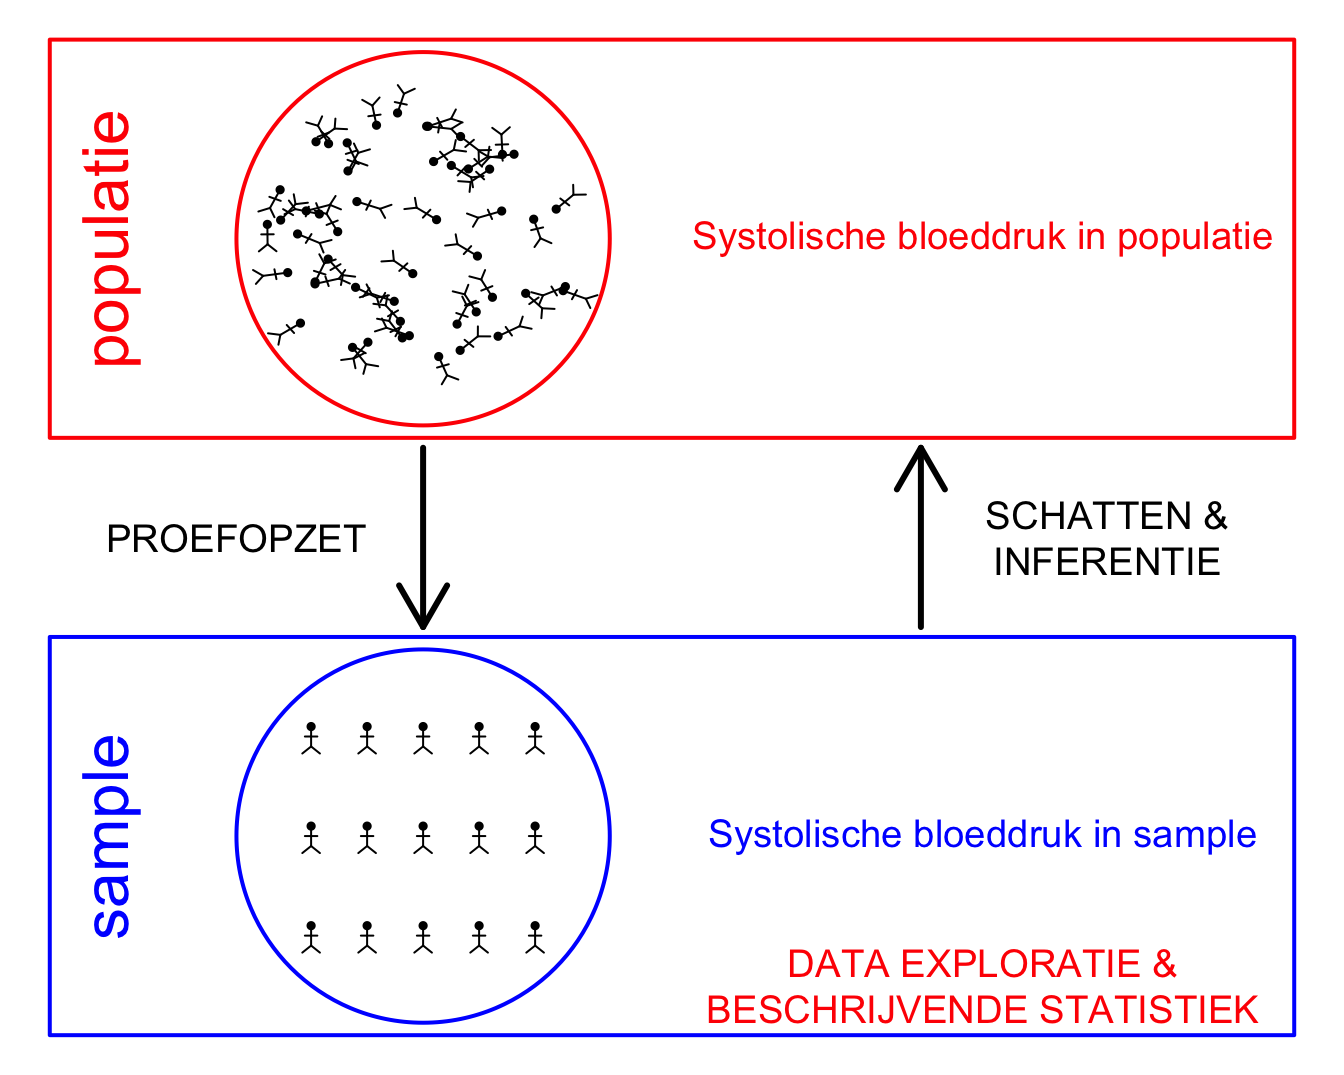
\includegraphics[width=1\linewidth]{Statistiek_2020_2021_files/figure-latex/pop2Samp2PopDataExpl-1} 

}

\caption{Verschillende stappen in een studie. In dit hoofdstuk ligt de focus op de data-exploratie en beschrijvende statistiek}\label{fig:pop2Samp2PopDataExpl}
\end{figure}

Dit hoofdstuk zullen werken rond een centrale dataset: de NHANES studie.

\begin{example}[NHANES studie]
\protect\hypertarget{exm:nhanesEx}{}{\label{exm:nhanesEx} \iffalse (NHANES studie) \fi{} }
\end{example}

De National Health and Nutrition Examination Survey
(NHANES) wordt sinds 1960 op regelmatige basis of genomen. In dit voorbeeld maken we gebruik van de gegevens die werden verzameld tussen 2009-2012 bij 10000 Amerikanen en die werden opgenomen in het R-pakket NHANES. Er werd een groot aantal fysische, demografische, nutritionele, levelsstijl en gezondheidskarakteristieken gecollecteerd in deze studie (zie Tabel \ref{tab:nhanesDatExpl}). Merk op dat ontbrekende waarnemingen hier gecodeerd worden a.d.h.b. de code \texttt{NA} (Not Available / Missing Value)

\textbf{Einde voorbeeld}

\begin{table}

\caption{\label{tab:nhanesDatExpl}Overzicht van een aantal variabelen uit de NHANES studie.}
\centering
\begin{tabular}[t]{rlrlrrrrrll}
\toprule
ID & Gender & Age & Race1 & Weight & Height & BMI & BPSysAve & TotChol & SmokeNow & Smoke100\\
\midrule
51624 & male & 34 & White & 87.4 & 164.7 & 32.22 & 113 & 3.49 & No & Yes\\
51625 & male & 4 & Other & 17.0 & 105.4 & 15.30 & NA & NA & NA & NA\\
51630 & female & 49 & White & 86.7 & 168.4 & 30.57 & 112 & 6.70 & Yes & Yes\\
51638 & male & 9 & White & 29.8 & 133.1 & 16.82 & 86 & 4.86 & NA & NA\\
51646 & male & 8 & White & 35.2 & 130.6 & 20.64 & 107 & 4.09 & NA & NA\\
\addlinespace
51647 & female & 45 & White & 75.7 & 166.7 & 27.24 & 118 & 5.82 & NA & No\\
\bottomrule
\end{tabular}
\end{table}

\hypertarget{sec:univar}{%
\section{Univariate beschrijving van de variabelen}\label{sec:univar}}

In de regel begint men met een \emph{univariate} inspectie: elke variabele
wordt apart onderzocht. Het is absoluut aan te raden om hierbij eerst alle
ruwe gegevens te bekijken door middel van grafieken (zie verder) alvorens
naar samenvattingsmaten (zoals het gemiddelde) over te stappen. Dit laat toe
om een idee te krijgen hoe de geobserveerde waarden van een veranderlijke
verdeeld zijn in de studiegroep (bvb. welke verdeling de bloeddrukmetingen in de studie hebben)
en of er eventuele \emph{uitschieters} (d.i. extreme
metingen of \emph{outliers}) zijn. Met outliers worden observaties
aangegeven die ten opzichte van de geobserveerde verdeling van de waarden in
de data set, extreem zijn, buitenbeentjes.

\begin{Shaded}
\begin{Highlighting}[]
\CommentTok{\# De data van de NHANES studie bevindt zich in het}
\CommentTok{\# R package NHANES}
\KeywordTok{library}\NormalTok{(NHANES)  }\CommentTok{\#laad NHANES package}

\CommentTok{\# NHANES is een data frame met de gegevens De rijen}
\CommentTok{\# bevatten informatie over elk subject De kolommen}
\CommentTok{\# de variabelen die werden geregistreerd vb}
\CommentTok{\# variabele Gender, BMI, ... Een variabele (kolom)}
\CommentTok{\# kan uit de dataframe worden gehaald door gebruik}
\CommentTok{\# van het $ teken en de naam van de variabele We}
\CommentTok{\# slaan de frequentietabel voor variable Gender op}
\CommentTok{\# in object \textquotesingle{}tab\textquotesingle{}}

\NormalTok{tab \textless{}{-}}\StringTok{ }\KeywordTok{table}\NormalTok{(NHANES}\OperatorTok{$}\NormalTok{Gender)}
\NormalTok{tab}
\end{Highlighting}
\end{Shaded}

\begin{verbatim}
## 
## female   male 
##   5020   4980
\end{verbatim}

We maken nu een barplot voor de variabele gender

\begin{enumerate}
\def\labelenumi{\arabic{enumi}.}
\tightlist
\item
  We pipen de NHANES data naar ggplot
\item
  Als aestetics definiëren we x=Gender
\item
  We voegen een laag met een barplot toe via de functie \texttt{geom\_bar}. We definiëren de kleur via het argument \texttt{fill}
\end{enumerate}

\begin{Shaded}
\begin{Highlighting}[]
\NormalTok{NHANES }\OperatorTok{\%\textgreater{}\%}\StringTok{ }\KeywordTok{ggplot}\NormalTok{(}\KeywordTok{aes}\NormalTok{(}\DataTypeTok{x =}\NormalTok{ Gender)) }\OperatorTok{+}\StringTok{ }\KeywordTok{geom\_bar}\NormalTok{(}\DataTypeTok{fill =} \StringTok{"steelblue"}\NormalTok{)}
\end{Highlighting}
\end{Shaded}

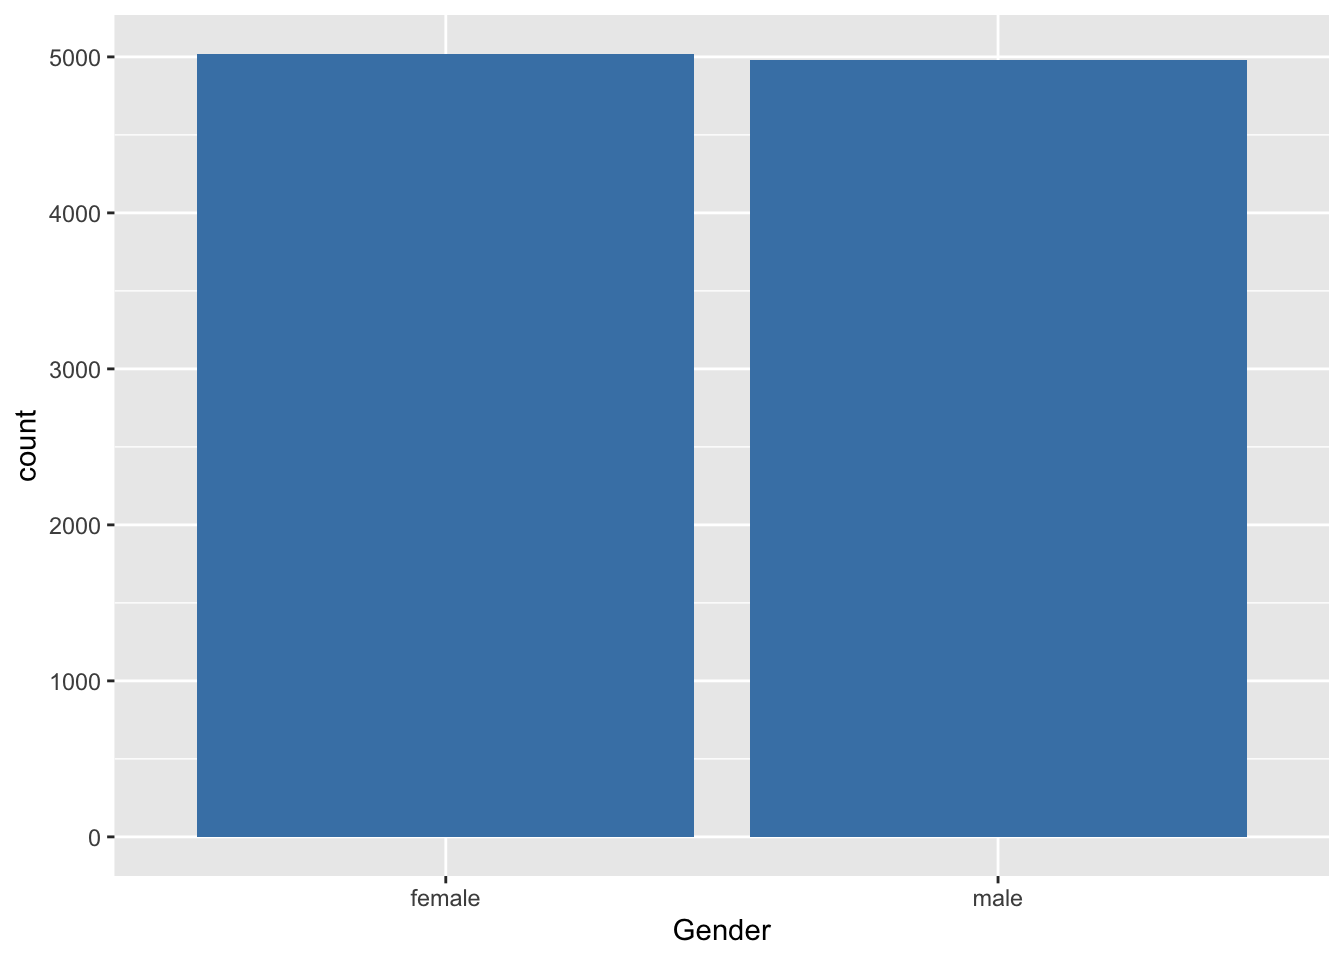
\includegraphics{Statistiek_2020_2021_files/figure-latex/unnamed-chunk-88-1.pdf}
Er zijn weinig methoden voorhanden om \emph{nominale} variabelen te
beschrijven. In Voorbeeld \ref{exm:nhanesEx} is de variable \emph{Gender}
kwalitatief nominaal.
Alles is gezegd over de verdeling van het geslacht als we weergeven hoeveel vrouwen en mannen zijn opgenomen in de studie.

We stellen vast dat 5020 van de 10000 subjecten, ofwel 50.2\% vrouwen in de studie zijn opgenomen.

Een staafdiagram geeft op de X-as de mogelijke uitkomsten van de variabele
aan (bvb. geslacht). Daarbovenop komt een staaf met hoogte evenredig aan
het totaal aantal keer dat die waarde voorkomt in de dataset. De staven staan los van elkaar met een breedte die constant is, maar verder willekeurig. Als de steekproef
representatief is voor de populatie, dan
krijgen we hier misschien een eerste impressie dat er iets meer vrouwen zijn in de populatie.

Voor \emph{numerieke continue variabelen} wordt het moeilijk om de
frequentie van alle uitkomstwaarden in een tabel te klasseren omdat veel
waarden hoogstens 1 keer voorkomen. Het \emph{tak-en-blad diagram} (in het
Engels: \emph{stem and leaf plot} is een middel om toch nog alle
uitkomsten weer te geven. Een voorbeeld is weergegeven in onderstaande R-output voor het BMI in de NHANES studie.

\begin{Shaded}
\begin{Highlighting}[]
\KeywordTok{stem}\NormalTok{(NHANES}\OperatorTok{$}\NormalTok{BMI)}
\end{Highlighting}
\end{Shaded}

\begin{verbatim}
## 
##   The decimal point is 1 digit(s) to the right of the |
## 
##   1 | 33333333333333333344444444444444444444444444444444444444444444444444+37
##   1 | 55555555555555555555555555555555555555555555555555555555555555555555+1389
##   2 | 00000000000000000000000000000000000000000000000000000000000000000000+2264
##   2 | 55555555555555555555555555555555555555555555555555555555555555555555+2610
##   3 | 00000000000000000000000000000000000000000000000000000000000000000000+1693
##   3 | 55555555555555555555555555555555555555555555555555555555555555555555+635
##   4 | 00000000000000000000000000000000000000000000000000000000000000000000+255
##   4 | 55555555555555555555555556666666666666666666666666666666666777777777+46
##   5 | 0000011111122222233333444444444444
##   5 | 5556677777789999
##   6 | 133444
##   6 | 567899
##   7 | 
##   7 | 
##   8 | 111
\end{verbatim}

Hier wordt van alle uitkomsten het eerste cijfer of de eerste paar cijfers
op een verticale lijn in volgorde uitgezet in de vorm van een boomstam.
Daaraan worden horizontaal de bladeren gehecht, met name de laatste cijfers
van de geobserveerde uitkomsten. De output geeft bijvoorbeeld aan dat er 3 personen zijn waarvan het afgeronde BMI 55 bedraagt, 2 personen met een afgerond BMI van 56, \ldots.
Gezien de studie zo groot is, is het tak-en-blad diagram niet erg praktisch voor dit voorbeeld.

In een tak-en-blad diagram krijgt men alle individuele uitkomsten nagenoeg
exact te zien, terwijl de vorm die het diagram aanneemt reeds een idee van
de verdeling geeft zoals in een histogram (zie verder). Een vuistregel om de
vorm van de verdeling het best te zien is het aantal takken ongeveer gelijk
te maken aan \(1 + \sqrt{n}\), waarbij \(n\) het aantal observaties voorstelt.
Dit aantal kan uiteraard aangepast worden aan de omstandigheden.
Een populair alternatief voor het tak en blad diagram is de \emph{eenvoudige frequentietabel}. Deze kan men bekomen door de continue variabele (bvb. BMI) om te zetten in een kwalitatieve ordinale variabele, waarvoor vervolgens een frequentietabel wordt weergegeven.

Het grafisch equivalent van dergelijke frequentietabel noemt een \emph{histogram}, hetgeen men in \texttt{ggplot} bekomt via

\begin{enumerate}
\def\labelenumi{\arabic{enumi}.}
\tightlist
\item
  Pipe de data van de NHANES study naar de \texttt{ggplot} functie
\item
  Selecteer de variable BMI als de data om in de x-coordinaat te visualiseren voor het aestetics argument van ggplot gebruik hiervoor de \texttt{aes} functie
\item
  Voeg een laag toe voor het histogram. Wanneer je geen aestetics \texttt{aes} meegeeft verkrijg je standaard absolute frequenties. Met \texttt{fill=..counts..} in de aestetics kan je de balken van het histogram inkleuren a.d.h.v. de absolute frequenties.
\item
  Indien je het wenst kan je op een histogram met densities ook nog een laag toevoegen met een niet parametrische densiteitsschatter voor de verdeling d.m.v. de \texttt{geom\_density} functie.
\end{enumerate}

\begin{Shaded}
\begin{Highlighting}[]
\NormalTok{NHANES }\OperatorTok{\%\textgreater{}\%}\StringTok{ }\KeywordTok{ggplot}\NormalTok{(}\KeywordTok{aes}\NormalTok{(}\DataTypeTok{x =}\NormalTok{ BMI)) }\OperatorTok{+}\StringTok{ }\KeywordTok{geom\_histogram}\NormalTok{(}\KeywordTok{aes}\NormalTok{(}\DataTypeTok{y =}\NormalTok{ ..density.., }
    \DataTypeTok{fill =}\NormalTok{ ..count..), }\DataTypeTok{bins =} \DecValTok{30}\NormalTok{) }\OperatorTok{+}\StringTok{ }\KeywordTok{geom\_density}\NormalTok{()}
\end{Highlighting}
\end{Shaded}

\begin{figure}

{\centering 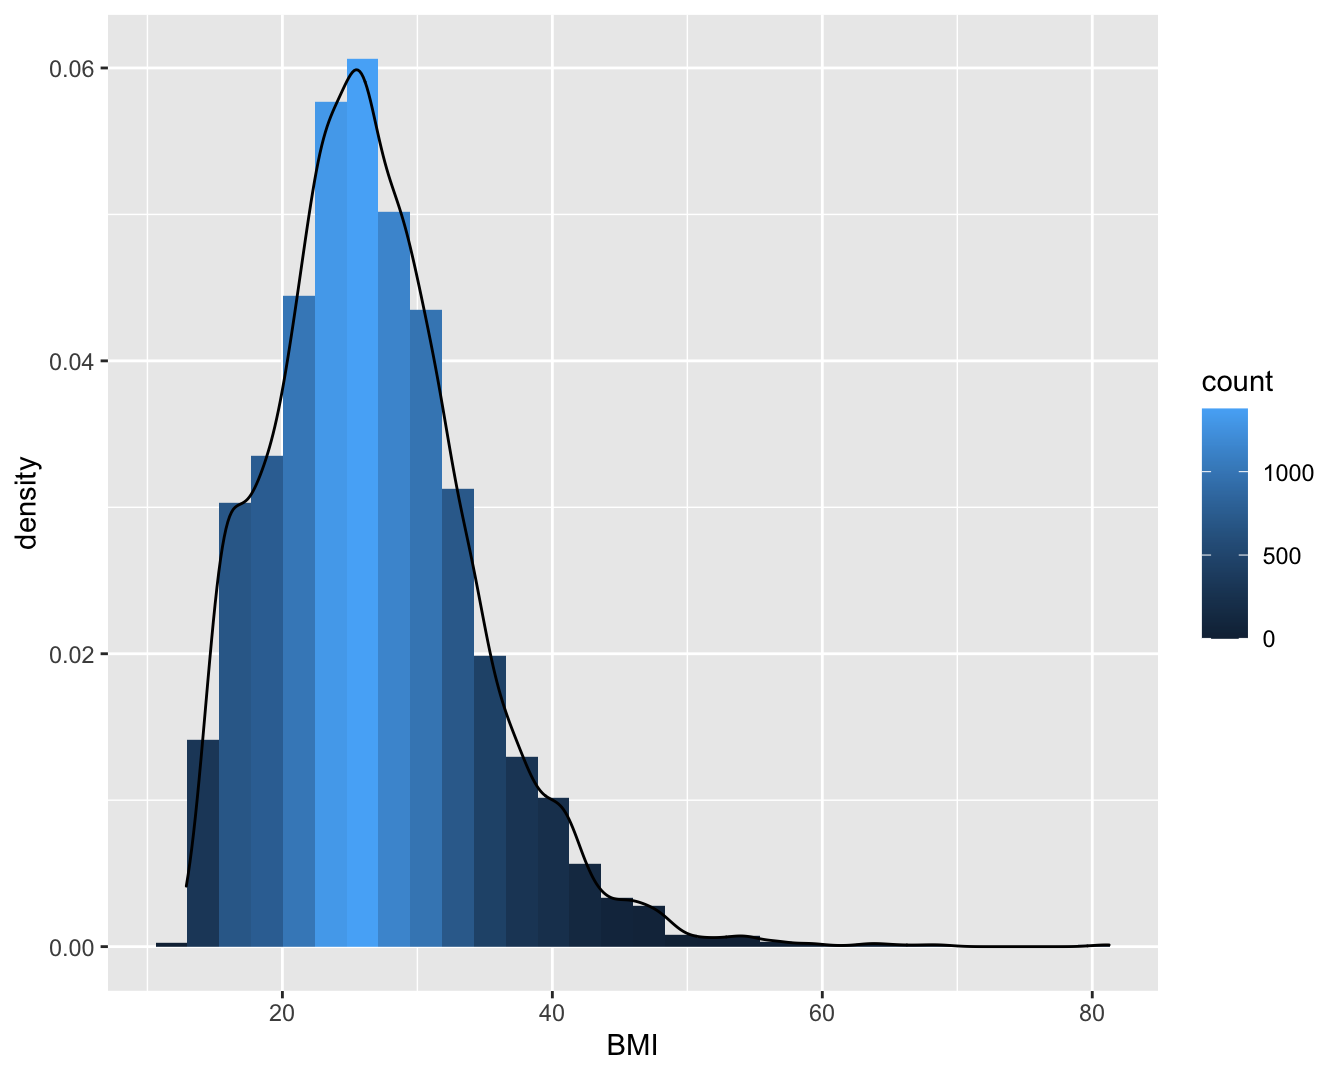
\includegraphics[width=1\linewidth]{Statistiek_2020_2021_files/figure-latex/histo-1} 

}

\caption{Histogram van het BMI in de NHANES studie.}\label{fig:histo}
\end{figure}

Wanneer alle klassen
een zelfde breedte hebben, worden de absolute of relatieve frequenties per
klasse weergegeven door de hoogte van de bijhorende kolom. Bij ongelijke
klassebreedtes is het de oppervlakte van de kolom die met de bijhorende
klassefrequentie correspondeert. Omdat een histogram met ongelijke
klassebreedtes moeilijker te interpreteren is, zijn histogrammen met gelijke
klassebreedtes vaak te verkiezen. Als histogrammen voor verschillende
groepen bekeken worden, vergemakkelijkt het gebruik van \emph{relatieve}
frequenties i.p.v. absolute frequenties de visuele vergelijkbaarheid.

Op het histogram in Figuur \ref{fig:histo} worden densiteiten
weergegeven en klassen met een breedte iets meer dan 5 eenheden.

De keuze van het aantal klassen is van belang bij een histogram. Als er te
weinig klassen zijn, dan gaat veel informatie verloren. Als er teveel zijn,
dan wordt het algemene patroon verdoezeld door een grote hoeveelheid overbodige
details. Gewoonlijk kiest men tussen 5 en 15 intervallen, maar de specifieke
keuze hangt af van het beeld van het histogram dat men te zien krijgt.

Een histogram is vooral geschikt om de distributie te schatten in grote datasets. Daar kan men dan veel intervallen gebruiken. Daarom heeft de ggplot functie standaard 30 intervallen.

Indien een voldoende aantal gegevens beschikbaar is, dan kan men een
gladdere indruk van de verdeling van de gegevens bekomen door een zogenaamde \emph{kernel density schatter} te bepalen. Zo'n schatter is een positieve functie die genormaliseerd is in die zin dat de oppervlakte onder de functie 1 is. Ze kan zo geïnterpreteerd worden dat de oppervlakte onder de functie tussen 2 punten \(a\) en \(b\) op de X-as, de kans voorstelt dat een lukrake meting in het interval \([a,b]\) gevonden wordt. Figuur \ref{fig:histo} toont een histogram met kernel density schatter van de het BMI.

De verdeling kan ook geëvalueerd worden aan de hand van een \emph{box-and-whisker-plot}, kortweg \emph{boxplot} genoemd. Deze is
meer compact dan een histogram en laat om die reden gemakkelijker
vergelijkingen tussen verschillende groepen toe (zie verder). Een Boxplot voor het BMI wordt getoond in Figuur \ref{fig:boxBMI}. De boxplot toont een
doos lopend van het 25\% tot 75\% percentiel met een lijntje ter hoogte van de
mediaan (het 50\% percentiel) en verder 2 snorharen. Die laatste kunnen in principe lopen tot het
minimum en maximum, of tot het 2.5\% en 97.5 \% of 5\% en 95\% percentiel.
R kiest voor de kleinste en de grootste geobserveerde waarde die geen
outlier of extreme waarde zijn. Een meting wordt hierbij een outlier genoemd
wanneer ze meer dan 1.5 keer de boxlengte beneden het eerste of boven het
derde kwartiel ligt. Een meting wordt een extreme waarde genoemd wanneer ze
meer dan 3 keer de boxlengte beneden het eerste of boven het derde kwartiel
ligt.

\begin{definition}[percentiel]
\protect\hypertarget{def:unnamed-chunk-90}{}{\label{def:unnamed-chunk-90} \iffalse (percentiel) \fi{} }
\end{definition}
Het \emph{25\% percentiel} of \emph{25\% kwantiel} \(x_{25}\) van een
reeks waarnemingen wordt gedefinieerd als een uitkomstwaarde \(x_{25}\) zodat
minstens \(25\%\) van die waarnemingen kleiner of gelijk zijn aan \(x_{25}\) en
minstens \(75\%\) van die waarnemingen groter of gelijk zijn aan \(x_{25}\). Het
\emph{75\% percentiel} of \emph{75\% kwantiel} van een reeks
waarnemingen definieert men als een uitkomstwaarde \(x_{75}\) zodat minstens 75\%
kleiner of gelijk zijn aan \(x_{75}\) en minstens \(25\%\) van die waarnemingen
groter of gelijk zijn aan \(x_{75}\). Algemeen wordt het \emph{\(k\%\)
percentiel} van een reeks waarnemingen gedefinieerd als een waarde (van \(x\))
waarvoor de cumulatieve frequentie gelijk is aan \(k/100.\) Als er meerdere
observaties aan voldoen neemt men vaak het gemiddelde van die waarden.

\textbf{Einde definitie}

In R kunnen die als volgt worden bekomen

\begin{Shaded}
\begin{Highlighting}[]
\KeywordTok{quantile}\NormalTok{(NHANES}\OperatorTok{$}\NormalTok{BMI, }\KeywordTok{c}\NormalTok{(}\FloatTok{0.25}\NormalTok{, }\FloatTok{0.5}\NormalTok{, }\FloatTok{0.75}\NormalTok{), }\DataTypeTok{na.rm =} \OtherTok{TRUE}\NormalTok{)}
\end{Highlighting}
\end{Shaded}

\begin{verbatim}
##   25%   50%   75% 
## 21.58 25.98 30.89
\end{verbatim}

\begin{figure}

{\centering 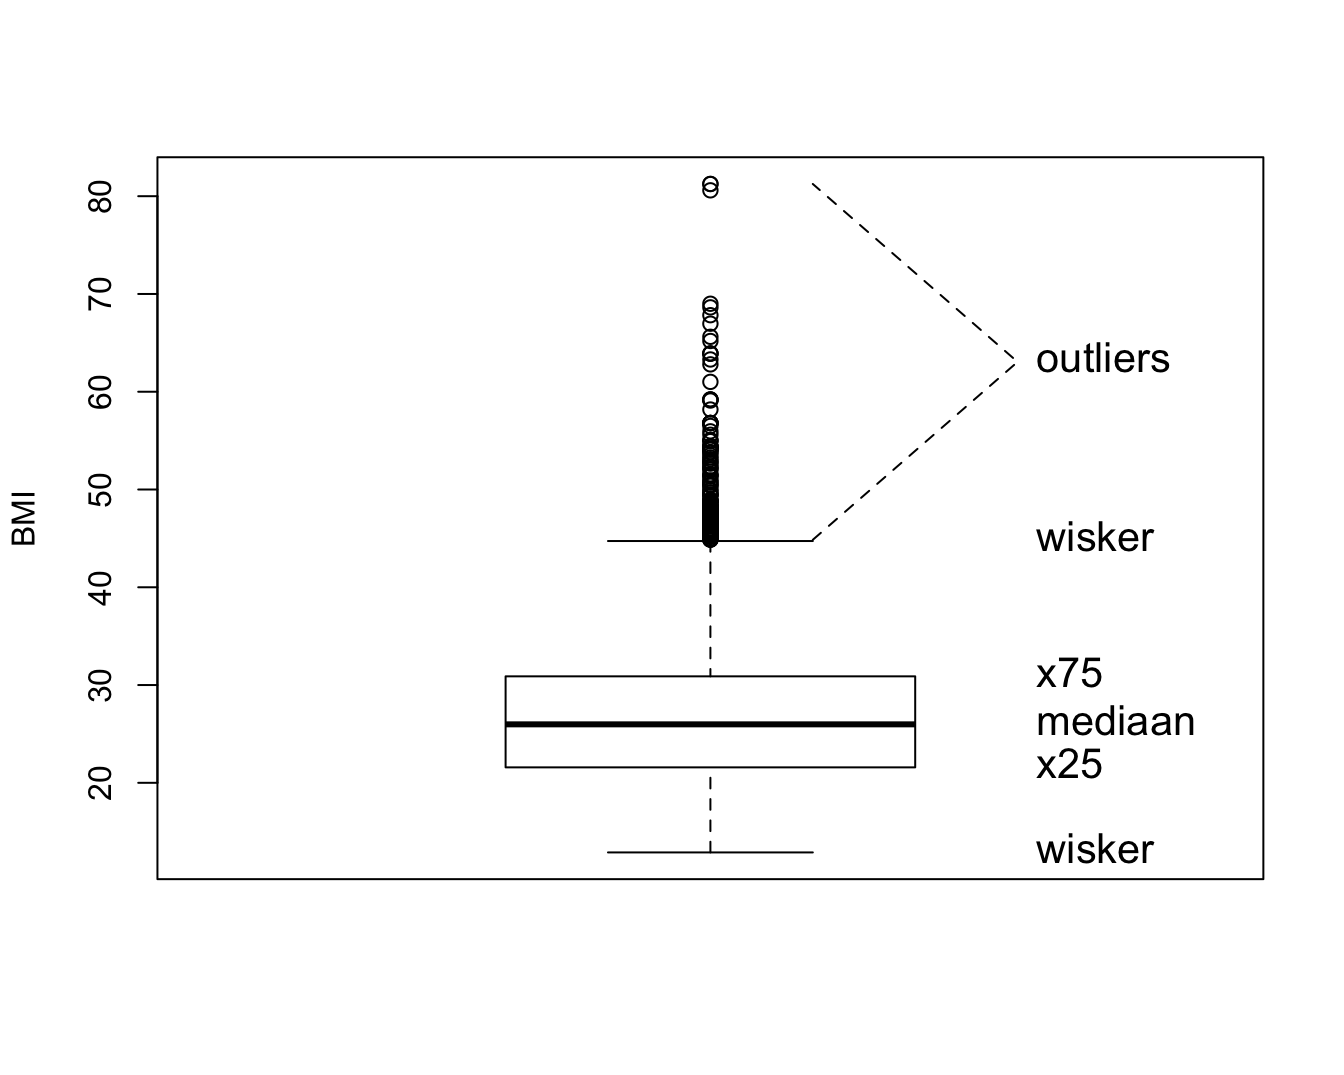
\includegraphics[width=1\linewidth]{Statistiek_2020_2021_files/figure-latex/boxBMI-1} 

}

\caption{Boxplot van BMI in de NHANES studie.}\label{fig:boxBMI}
\end{figure}

In ggplot maak je de boxplot als volgt:

\begin{Shaded}
\begin{Highlighting}[]
\NormalTok{NHANES }\OperatorTok{\%\textgreater{}\%}\StringTok{ }\KeywordTok{ggplot}\NormalTok{(}\KeywordTok{aes}\NormalTok{(}\DataTypeTok{x =} \StringTok{""}\NormalTok{, }\DataTypeTok{y =}\NormalTok{ BMI)) }\OperatorTok{+}\StringTok{ }\KeywordTok{geom\_boxplot}\NormalTok{()}
\end{Highlighting}
\end{Shaded}

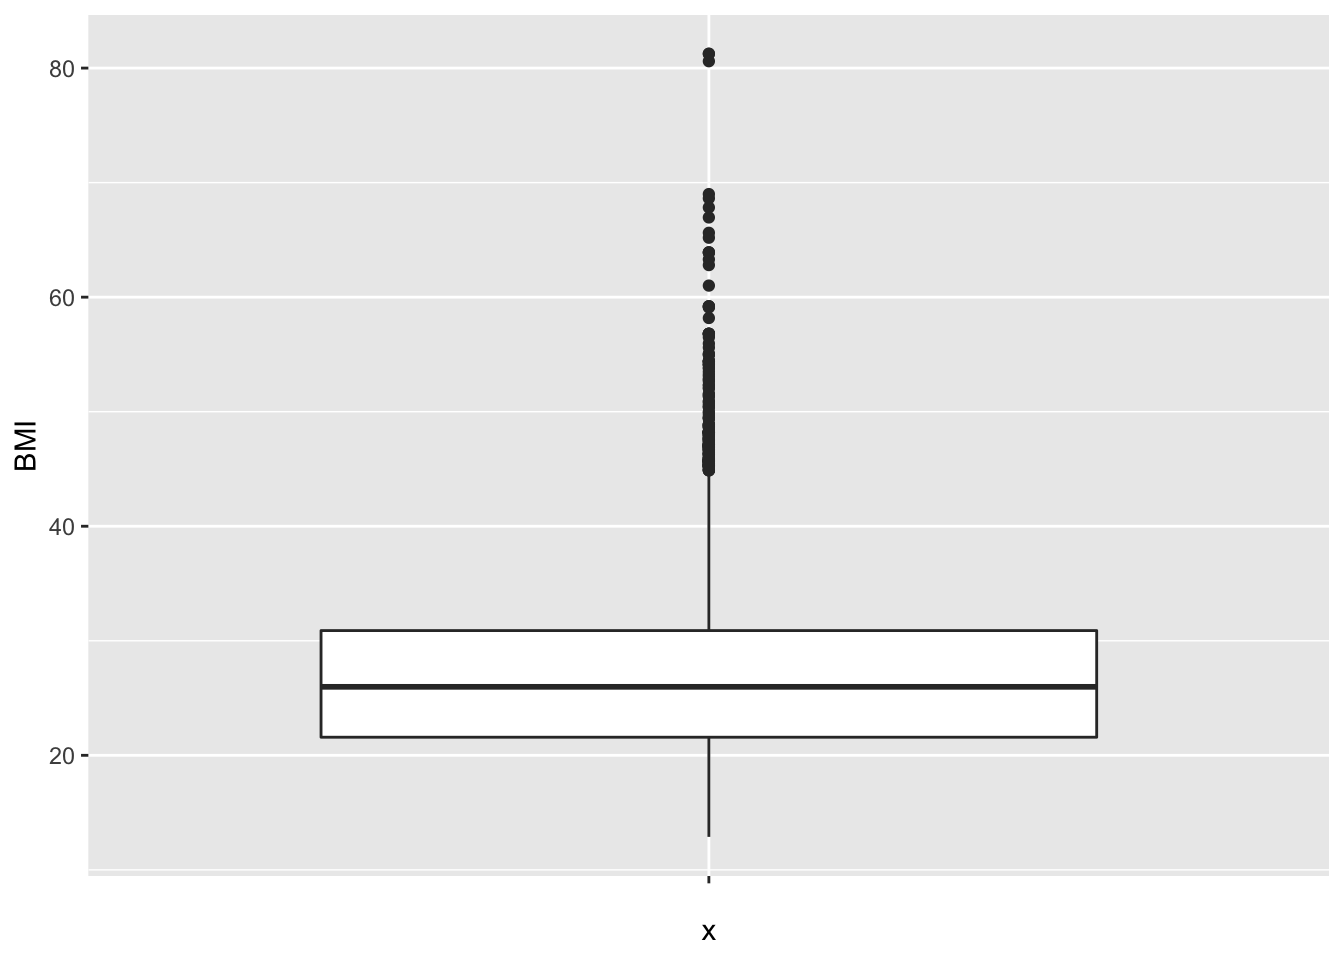
\includegraphics{Statistiek_2020_2021_files/figure-latex/unnamed-chunk-92-1.pdf}

Bij de inspectie van een dataset speelt het detecteren van outliers in het
algemeen een belangrijke rol. Ze kunnen wijzen op fouten, zoals tikfouten of
andere fouten die gecheckt en gecorrigeerd moeten worden. Als het geen
foutief genoteerde waarden zijn, dan kan het soms wijzen op een subject dat niet
echt in de studiepopulatie thuis hoort. Als het in
alle opzichten om een bona fide waarde gaat, dan nog is het belangrijk om
outliers te detecteren: ze kunnen zeer invloedrijk zijn op de schatting van
statistische parameters (zie Sectie \ref{sec:summarize}). Als de conclusies
van een studie anders liggen met of zonder inclusie van de outlier, dan is
dit een ongewenst fenomeen. Men wil immers nooit dat 1 observatie beslissend
is voor de conclusies. Dit soort onzekerheid ondermijnt de geloofwaardigheid
van de onderzoeksresultaten en vraagt om verdere studie. Binnen de
statistiek bestaat een grote waaier aan technieken, zogenaamde
\emph{robuuste statistische technieken}, die erop gericht zijn om de invloed van
outliers te minimaliseren. In deze cursus gaan we hier slechts in zeer
beperkte mate op in (zie Sectie \ref{sec:summarize}, mediaan).

\hypertarget{sec:summarize}{%
\section{Samenvattingsmaten voor continue variabelen}\label{sec:summarize}}

Een histogram levert reeds een sterke samenvatting van de geobserveerde,
continue gegevens, maar in wetenschappelijke rapporten is er zelden
plaats om per geobserveerde variabele dergelijke grafiek voor te stellen. Om
die reden is vaak een veel drastischere samenvattingsmaat noodzakelijk. In deze
sectie geven we aan hoe de centrale locatie van de gegevens kan beschreven
worden, alsook de spreiding van die gegevens rond hun centrale locatie.

\hypertarget{maten-voor-de-centrale-ligging}{%
\subsection{Maten voor de centrale ligging}\label{maten-voor-de-centrale-ligging}}

\begin{definition}[rekenkundig gemiddelde]
\protect\hypertarget{def:unnamed-chunk-93}{}{\label{def:unnamed-chunk-93} \iffalse (rekenkundig gemiddelde) \fi{} }
\end{definition}
Het \textbf{(rekenkundig) gemiddelde} \(\overline{x}\) (spreek uit: \emph{x-streep}
of \emph{x-bar}) van een reeks waarnemingen \(x_i, i=1, 2, \dots, n\) is per
definitie de som van de observaties gedeeld door hun aantal \(n\):

\[\overline{x}= \frac{x_1 + x_2 + \dots + x_n}{n} =\sum_{i=1}^n x_i \frac{1}{n} \]

\textbf{Einde definitie}

Merk op dat het rekenkundig gemiddelde ook verkregen zou worden als gemiddelde voor een discrete distributie met kansen van 1/n op elke waarde uit de steekproef.
Wanneer we het steekproefgemiddelde gebruiken dan schatten we de distributie in de populatie als het ware aan de hand van de empirische distributie van de data. We maken dus geen distributionele veronderstellingen hiervoor.

Een groot voordeel van het gemiddelde als een maat voor de centrale locatie
van de observaties is dat het alle data-waarden efficiënt gebruikt vanuit
statistisch perspectief. Dit wil zeggen dat ze (onder bepaalde statistische modellen)
het maximum aan informatie
uit de gegevens haalt en om die reden relatief gezien zeer stabiel blijft
wanneer ze herberekend wordt op basis van een nieuwe, even grote steekproef
die onder identieke omstandigheden werd bekomen. Bovendien beschrijft het
gemiddelde ook verschillende belangrijke modellen voor de verdeling van de
gegevens, zoals de Normale verdeling (zie Sectie \ref{sec:normal}). Een
groot nadeel van het gemiddelde is dat het zeer gevoelig is aan de
aanwezigheid van outliers in de dataset. Om die reden is het vooral een
interessante maat van locatie wanneer de verdeling van de observaties (zoals
weergegeven door bijvoorbeeld een histogram) min of meer symmetrisch is.

\begin{Shaded}
\begin{Highlighting}[]
\KeywordTok{mean}\NormalTok{(NHANES}\OperatorTok{$}\NormalTok{BMI, }\DataTypeTok{na.rm =} \OtherTok{TRUE}\NormalTok{)}
\end{Highlighting}
\end{Shaded}

\begin{verbatim}
## [1] 26.66014
\end{verbatim}

\begin{Shaded}
\begin{Highlighting}[]
\CommentTok{\# opnieuw is de na.rm statement hier nodig omdat}
\CommentTok{\# ontbrekende waarden voorkomen.}
\end{Highlighting}
\end{Shaded}

\emph{Indien men de grootste observatie (81.25) vervangt door 8125 om als het ware ene tikfout voor te stellen, dan wijzigt het rekenkundig gemiddelde naar 27.5 en dat terwijl er bijna 10000 BMI metingen zijn. Merk op dat het gemiddelde vrij sterk beïnvloed kan worden door één outlier.}

\textbf{Eigenschap}

Als alle uitkomsten \(x_i\) met een willekeurige constante \(a\)
worden vermenigvuldigd, dan ook het gemiddelde van die reeks uitkomsten. Als
bij alle uitkomsten een constante \(a\) wordt opgeteld, dan ook bij het
gemiddelde van die reeks uitkomsten. Formeel betekent dit:

\begin{eqnarray*}
\overline{ax} &= &a \overline{x} \\
\overline{a + x} &= &a + \overline{x}
\end{eqnarray*}

Voor 2 reeksen getallen \(x_i\) en \(y_i\), \(i=1,...,n\), geldt dat het
gemiddelde van de som van de observaties gelijk is aan de som van hun
gemiddelden:

\begin{equation*}
\overline{x + y} = \overline{x} + \overline{y}.
\end{equation*}

Als de gegevens \(x_i\) enkel de waarden 0 of 1 aannemen, dan is \(\overline{x}\)
de proportie subjecten voor wie de waarde 1 werd geobserveerd. Immers, zij \(n_1\) het aantal subjecten binnen de groep van \(n\) subjecten waarvoor de
waarde 1 werd geobserveerd, dan is

\begin{equation*}
\overline{x}= \sum_{i=1}^n \frac{x_i}{n} = \frac{n_1}{n}.
\end{equation*}

Bijvoorbeeld, als we de variabele \textbf{Gender} zó
coderen dat mannen een waarde 0 aannemen en vrouwen een waarde 1, dan is het
gemiddelde van de variabele \textbf{Gender} gelijk aan 50.2\%, hetgeen de proportie is van het aantal vrouwen in de studie. Een percentage kan dus
steeds opgevat worden als het gemiddelde van een geschikte variabele.

\textbf{Einde eigenschap}

Een centrale maat die robuuster reageert dan het gemiddelde, d.w.z. minder
of niet gevoelig is aan outliers, is de \emph{mediaan} of het \emph{50\% percentiel}.

\begin{definition}[mediaan]
\protect\hypertarget{def:unnamed-chunk-95}{}{\label{def:unnamed-chunk-95} \iffalse (mediaan) \fi{} }
\end{definition}
De \textbf{mediaan}, het \textbf{50\% percentiel} of het \textbf{50\%
kwantiel} \(x_{50}\) van een reeks waarnemingen \(x_i, i=1, 2, \dots, n\) is per
definitie een uitkomstwaarde \(x_{50}\) zodat minstens \(50\%\) van die
waarnemingen groter of gelijk zijn aan \(x_{50}\) en minstens \(50\%\) van die
waarnemingen kleiner of gelijk zijn aan \(x_{50}\).

\textbf{Einde definitie}

Om de mediaan te schatten, rangschikt men eerst de gegevens volgens grootte.
Als het aantal observaties \(n\) oneven is, dan is een schatting voor de
mediaan de middelste waarneming. Indien \(n\) even is, dan zijn er 2 middelste
waarnemingen en schat men de mediaan (meestal) als hun gemiddelde. Een
voordeel van de mediaan is dat ze niet gevoelig is aan outliers. In het bijzonder kan
ze vaak nuttig aangewend worden wanneer sommige gegevens \emph{gecensureerd}
zijn. Dit wil zeggen dat men voor een aantal gegevens enkel weet dat ze
boven of onder een bepaalde drempelwaarde liggen.

\begin{Shaded}
\begin{Highlighting}[]
\KeywordTok{median}\NormalTok{(NHANES}\OperatorTok{$}\NormalTok{BMI, }\DataTypeTok{na.rm =} \OtherTok{TRUE}\NormalTok{)}
\end{Highlighting}
\end{Shaded}

\begin{verbatim}
## [1] 25.98
\end{verbatim}

\begin{Shaded}
\begin{Highlighting}[]
\CommentTok{\# Merk op dat we hier gebruik maken van het}
\CommentTok{\# argument na.rm=TRUE Dit komt omdat we niet}
\CommentTok{\# beschikken over het BMI voor elke persoon:}
\CommentTok{\# ontbrekende waarnemingen Die worden in R als een}
\CommentTok{\# NA voorgesteld Als we het argument na.rm=TRUE}
\CommentTok{\# gebruiken wordt de mediaan berekend op basis van}
\CommentTok{\# de beschikbare observaties}
\end{Highlighting}
\end{Shaded}

Indien men de grootste observatie (81.25) vervangt 8125, dan wijzigt de mediaan niet.
Merk ook op dat de mediaan lager is dan het gemiddelde, hij is minder gevoelig voor de outliers in de dataset.

\begin{definition}[modus]
\protect\hypertarget{def:unnamed-chunk-97}{}{\label{def:unnamed-chunk-97} \iffalse (modus) \fi{} }
\end{definition}
De \textbf{modus} van een reeks observaties is de waarde die het meest
frequent is, of wanneer de gegevens gegroepeerd worden, de klasse met de
hoogste frequentie.

\textbf{Einde definitie}

De modus wordt niet vaak gebruikt in statistische analyse omdat haar waarde
sterk afhangt van de nauwkeurigheid waarmee de gegevens werden gemeten. Zo
is de modus van de reeks observaties \(1, 1, 1, 1.5, 1.75, 1.9, 2, 2.1, 2.4\)
gelijk aan 1, maar wordt ze 2 wanneer alle observaties afgerond worden tot
gehele getallen. Bovendien is de modus niet eenvoudig te schatten voor
continue data waar de frequentie van elke geobserveerde waarde meestal 1 is.
De modus is daarom het meest zinvol voor kwalitatieve en discrete numerieke
gegevens, waar ze de meest frequente klasse aanduidt.

Als de observaties uit een \emph{symmetrische verdeling} afkomstig zijn,
vallen de mediaan en het gemiddelde nagenoeg samen (als de geobserveerde
verdeling perfect symmetrisch is, vallen ze theoretisch exact samen).
De beste schatter voor het centrum van de verdeling op basis van de beschikbare
steekproef is dan het gemiddelde eerder dan de mediaan van die observaties.
Inderdaad, als men telkens opnieuw een lukrake steekproef neemt uit de
gegeven studiepopulatie en voor elke steekproef het gemiddelde en de mediaan
berekent, dan zal het gemiddelde minder variëren van steekproef tot
steekproef dan de mediaan. Ze is bijgevolg stabieler en wordt daarom een
\emph{meer precieze schatter} genoemd. Intuïtief kan men begrijpen dat
het gemiddelde meer informatie uit de gegevens gebruikt: niet alleen of iets
groter of kleiner is dan \(x_{50}\) maar ook hoeveel groter of kleiner de
exacte waarde van elke observatie is, wordt in de berekening betrokken.

\begin{definition}[scheve verdeling]
\protect\hypertarget{def:unnamed-chunk-98}{}{\label{def:unnamed-chunk-98} \iffalse (scheve verdeling) \fi{} }
\end{definition}
Een niet-symmetrische verdeling wordt \textbf{scheef} genoemd. Als de
waarden rechts van de mediaan verder uitlopen dan links, dan is de verdeling
\emph{scheef naar rechts} (in het Engels: \emph{positively skew}) en is
het gemiddelde (meestal) groter dan de mediaan. Als de waarden links van de
mediaan verder uitlopen dan rechts, dan is de verdeling \emph{scheef naar
links} (in het Engels: \emph{negatively skew}) en is het gemiddelde
(meestal) kleiner dan de mediaan.

\textbf{Einde definitie}

Voor een niet-symmetrische verdeling is de mediaan veelal een beter
interpreteerbare maat dan het gemiddelde omdat ze minder beïnvloed is
door de staarten van de verdeling en daarom beter het centrum van de
verdeling aanduidt. Maar in sommige gevallen, zoals bijvoorbeeld voor `de
gemiddelde opbrengst per week', blijft het gemiddelde zinvol omdat het
meteen verwijst naar de totale opbrengst over alle weken (gelijk aan \(n\)
keer het gemiddelde als \(n\) weken werden geobserveerd). Ook voor
kwalitatieve variabelen kan een gemiddelde zinvol zijn. Voor binaire
nominale variabelen die als 1 of 0 gecodeerd zijn, geeft het gemiddelde
immers het percentage observaties gelijk aan 1 weer. Voor ordinale
variabelen die bijvoorbeeld gecodeerd zijn als \(1, 2, 3, ...\) levert het
gemiddelde soms nuttigere informatie dan de mediaan. Niettemin berust het
dan op de impliciete onderstelling dat een wijziging van score van 1 naar 2
even belangrijk is als een wijziging van 2 naar 3.

Om scheve verdelingen in een paar woorden te beschrijven is het vaak nuttig
om

\begin{itemize}
\tightlist
\item
  ofwel de gegevens te beschrijven in termen van percentielen,
\item
  ofwel de gegevens te transformeren naar een andere schaal (bvb. door
  logaritmen te nemen), zodat ze op de nieuwe schaal bij benadering
  symmetrisch verdeeld zijn.
\end{itemize}

Wanneer het gemiddelde groter is dan de mediaan en alle metingen positief zijn (vb concentraties, BMI), dan is een logaritmische
transformatie van de gegevens vaak nuttig om de scheefheid weg te nemen. In
dit geval is vooral het \emph{geometrisch gemiddelde} interessant.

\begin{definition}[geometrisch gemiddelde]
\protect\hypertarget{def:unnamed-chunk-99}{}{\label{def:unnamed-chunk-99} \iffalse (geometrisch gemiddelde) \fi{} }
\end{definition}
Het \textbf{geometrische gemiddelde} van een reeks waarnemingen \(x_i, i=1, 2, \dots, n\) ontstaat door er de natuurlijke logaritme van te berekenen, het
gemiddelde hiervan te nemen en dit vervolgens terug te transformeren naar de
originele schaal door er de exponentiële functie van te nemen:

\begin{equation*}
\sqrt[n]{\prod\limits_{i=1}^n x_i} = \exp\left\{\frac{1}{n} \sum_{i=1}^n \log(x_i)\right\}
\end{equation*}

\textbf{Einde definitie}

\begin{itemize}
\item
  Geometrisch gemiddelde ligt dichter bij de mediaan dan het gemiddelde
\item
  log-transformatie verwijdert scheefheid
\item
  Is vaak een meer geschikte maat voor centrale locatie dan de mediaan:
\end{itemize}

\begin{enumerate}
\def\labelenumi{\arabic{enumi}.}
\tightlist
\item
  Gebruikt alle observatie: is meer precies
\item
  Is het rekenkundig gemiddelde van log-transformeerde data \(\rightarrow\) klassieke statistische methoden kunnen direct worden gebruikt, b.v. hypothese testen en betrouwbaarheidsintervallen (zie hoofdstuk 5)
\item
  Veel biologische en chemische variabelen zoals concentraties, intensiteiten, etc kunnen niet negatief zijn.
\item
  Verschillen op log schaal hebben de betekenis van een \texttt{log\ fold\ change}:
\end{enumerate}

\[
\log (B) - \log(A)= \log(\frac{B}{A})=\log(FC_\text{B vs A})
\]

\begin{itemize}
\item
  In Genomics wordt de \(\log_2\) transformatie veel gebruikt.
\item
  Een verschil van 1 op \(\log_2\) schaal betekent een verdubbeling op de originele schaal \(FC=2\).
\end{itemize}

\begin{Shaded}
\begin{Highlighting}[]
\NormalTok{logSummary \textless{}{-}}\StringTok{ }\NormalTok{NHANES }\OperatorTok{\%\textgreater{}\%}\StringTok{ }\KeywordTok{filter}\NormalTok{(Gender }\OperatorTok{==}\StringTok{ "female"}\NormalTok{) }\OperatorTok{\%\textgreater{}\%}\StringTok{ }
\StringTok{    }\KeywordTok{summarize}\NormalTok{(}\DataTypeTok{logMean =} \KeywordTok{mean}\NormalTok{(BMI }\OperatorTok{\%\textgreater{}\%}\StringTok{ }\NormalTok{log2, }\DataTypeTok{na.rm =} \OtherTok{TRUE}\NormalTok{), }
        \DataTypeTok{sd =} \KeywordTok{sd}\NormalTok{(BMI }\OperatorTok{\%\textgreater{}\%}\StringTok{ }\NormalTok{log2, }\DataTypeTok{na.rm =} \OtherTok{TRUE}\NormalTok{), }\DataTypeTok{mean =} \KeywordTok{mean}\NormalTok{(BMI, }
            \DataTypeTok{na.rm =} \OtherTok{TRUE}\NormalTok{), }\DataTypeTok{median =} \KeywordTok{median}\NormalTok{(BMI, }\DataTypeTok{na.rm =} \OtherTok{TRUE}\NormalTok{)) }\OperatorTok{\%\textgreater{}\%}\StringTok{ }
\StringTok{    }\KeywordTok{mutate}\NormalTok{(}\DataTypeTok{geoMean =} \DecValTok{2}\OperatorTok{\^{}}\NormalTok{logMean)}

\NormalTok{NHANES }\OperatorTok{\%\textgreater{}\%}\StringTok{ }\KeywordTok{filter}\NormalTok{(Gender }\OperatorTok{==}\StringTok{ "female"}\NormalTok{) }\OperatorTok{\%\textgreater{}\%}\StringTok{ }\KeywordTok{ggplot}\NormalTok{(}\KeywordTok{aes}\NormalTok{(}\DataTypeTok{x =}\NormalTok{ BMI }\OperatorTok{\%\textgreater{}\%}\StringTok{ }
\StringTok{    }\NormalTok{log2)) }\OperatorTok{+}\StringTok{ }\KeywordTok{geom\_histogram}\NormalTok{(}\KeywordTok{aes}\NormalTok{(}\DataTypeTok{y =}\NormalTok{ ..density.., }\DataTypeTok{fill =}\NormalTok{ ..count..), }
    \DataTypeTok{bins =} \DecValTok{30}\NormalTok{) }\OperatorTok{+}\StringTok{ }\KeywordTok{geom\_density}\NormalTok{() }\OperatorTok{+}\StringTok{ }\KeywordTok{stat\_function}\NormalTok{(}\DataTypeTok{fun =}\NormalTok{ dnorm, }
    \DataTypeTok{color =} \StringTok{"red"}\NormalTok{, }\DataTypeTok{args =} \KeywordTok{list}\NormalTok{(}\DataTypeTok{mean =}\NormalTok{ logSummary}\OperatorTok{$}\NormalTok{logMean, }
        \DataTypeTok{sd =}\NormalTok{ logSummary}\OperatorTok{$}\NormalTok{sd))}
\end{Highlighting}
\end{Shaded}

\begin{figure}

{\centering 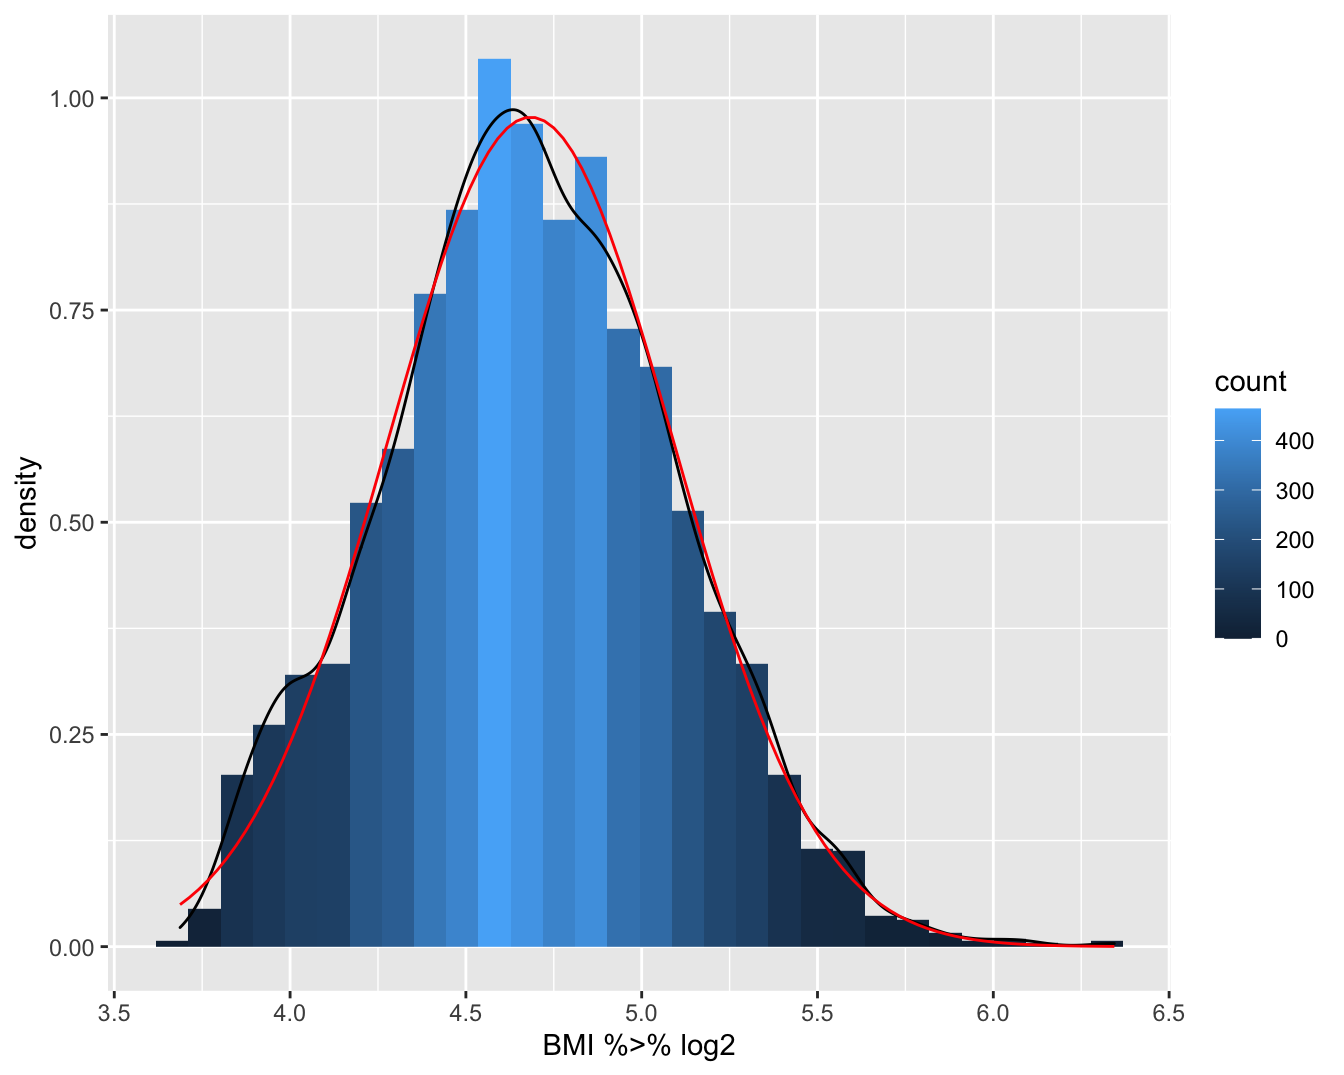
\includegraphics[width=1\linewidth]{Statistiek_2020_2021_files/figure-latex/histLogBMI-1} 

}

\caption{Boxplot van BMI en log(BMI) in de NHANES studie.}\label{fig:histLogBMI}
\end{figure}

\begin{Shaded}
\begin{Highlighting}[]
\NormalTok{logSummary}
\end{Highlighting}
\end{Shaded}

\begin{verbatim}
## # A tibble: 1 x 5
##   logMean    sd  mean median geoMean
##     <dbl> <dbl> <dbl>  <dbl>   <dbl>
## 1    4.68 0.408  26.8   25.6    25.7
\end{verbatim}

In situaties waar de log-transformatie inderdaad de scheefheid wegneemt, zal
het geometrisch gemiddelde dichter bij de mediaan liggen dan het gemiddelde.
Wanneer de verdeling scheef is, is ze soms zelfs een nuttigere maat voor centrale
locatie dan de mediaan:

\begin{enumerate}
\def\labelenumi{\arabic{enumi}.}
\item
  omdat ze ook gebruik maakt van de exacte waarden van de observaties en
  daarom doorgaans preciezer is dan de mediaan;
\item
  omdat ze, op een transformatie na, berekend wordt als een rekenkundig
  gemiddelde (weliswaar van de logaritmisch getransformeerde observaties) en
  algemene statistische technieken voor een gemiddelde (zoals
  betrouwbaarheidsintervallen (zie volgende hoofdstukken) en toetsen van hypothesen (zie volgende hoofdstukken) daardoor vrijwel rechtstreeks
  toepasbaar zijn voor geometrische gemiddelden.
\end{enumerate}

\begin{example}[BMI]
\protect\hypertarget{exm:unnamed-chunk-100}{}{\label{exm:unnamed-chunk-100} \iffalse (BMI) \fi{} }
\end{example}
Het gemiddelde en mediane BMI bedraagt 26.66 en 25.98 , respectievelijk. Het gemiddelde is hier groter dan de mediaan omdat de BMI scheef verdeeld is naar rechts (zie Figuur \ref{fig:histLogBMI}). De verdeling wordt meer symmetrisch na log-transformatie. Het gemiddelde en mediane log-BMI liggen ook dichter bij elkaar en bedragen respectievelijk 3.25 en 3.26. De geometrisch gemiddelde BMI-concentratie bekomen we door de exponentiële functie te evalueren in 3.25, hetgeen ons 25.69 oplevert. Merk op dat dit inderdaad beter met de mediaan overeenstemt dan het rekenkundig gemiddelde.

\textbf{Einde voorbeeld}

Tot slot, vooraleer een eenvoudige maat voor de centrale ligging (en
spreiding) te construeren of interpreteren, is het goed om altijd eerst de
volledige verdeling te bekijken! Immers, stel dat men het gemiddelde of
mediaan berekent van gegevens uit een bimodale verdeling (d.i. een verdeling
met 2 modi, voor bvb. zieken en niet-zieke dieren). Dan kan het gemiddelde of
mediaan makkelijk een zeer zeldzame waarde aannemen die geenszins in de
buurt van 1 van beide maxima ligt.

\hypertarget{subsec:spreiding}{%
\subsection{Spreidingsmaten}\label{subsec:spreiding}}

Nadat de centrale ligging van de gegevens werd bepaald, is men in tweede
instantie geïnteresseerd in de spreiding van de gegevens rond
die centrale waarde. Er zijn verschillende redenen waarom daar interesse in bestaat:

\begin{enumerate}
\def\labelenumi{\arabic{enumi}.}
\tightlist
\item
  Om risico's te berekenen (zie Sectie \ref{sec:normal}) volstaat het niet om de centrale locatie van de gegevens te kennen, maar moet men bovendien weten hoeveel de gegevens rond die waarde variëren. Inderdaad, stel dat men wenst te weten welk percentage van de subjecten een BMI heeft van boven de 35. Wetende dat een geometrisch gemiddelde van 25.69 wordt geobserveerd, zal dat percentage relatief hoog zijn wanneer de metingen zeer gespreid zijn en relatief laag anders.
\item
  Veldbiologen zijn vaak geïnteresseerd in de mate waarin dieren of planten verspreid zijn over een zeker studiegebied. Op die manier kunnen ze immers leren over de relaties tussen individuen onderling en met hun omgeving. Daartoe zal men in de praktijk op verschillende plaatsen in het studiegebied tellingen maken van het aantal individuen op die plaats. Men kan aantonen dat, onder bepaalde veronderstellingen, individuen lukraak verspreid zijn over het studiegebied wanneer de spreiding op die tellingen, zoals gemeten door de variantie (zie verder), van dezelfde grootte-orde is als de gemiddelde telling. Indien de spreiding groter is, dan hebben individuen de neiging om zich te groeperen. Andersom, indien de spreiding op die tellingen lager is dan de gemiddelde telling, dan zijn de individuen zeer uniform verdeeld over het studiegebied.
\item
  Stel dat men een zekere uitkomst (bvb. het aantal species ongewervelde dieren in een stuk bodemkorst) wenst te vergelijken tussen 2 groepen (bvb. gebieden met en zonder bosbrand), dan zal men een duidelijk beeld van het groepseffect krijgen wanneer de uitkomst weinig gespreid is, maar een veel minder duidelijk beeld wanneer de gegevens meer chaotisch (en dus meer gespreid) zijn. Om uit te maken of een interventie-effect toevallig of systematisch is, moet men daarom een idee hebben van de spreiding op de gegevens.
\end{enumerate}

Dat uitkomsten variëren tussen individuen en binnen individuen omwille van
allerlei redenen ligt aan de basis van de statistische analyse van veel
fenomenen. Het goed beschrijven van variatie naast de centrale locatie van
de gegevens is daarom belangrijk! Hierbij zal men typisch een
onderscheid maken tussen variatie die men kan verklaren (door middel van
karakteristieken, zoals bijvoorbeeld de leeftijd, van de bestudeerde individuen) en onverklaarde variatie. We gaan
dieper in op dit onderscheid in Hoofdstuk \ref{chap:linReg} rond lineaire regressie.

Variatie betekent dat niet alle observaties \(x_i\) gelijk zijn aan het
gemiddelde \(\overline{x}\). De afwijking \(x_i - \bar{x}\) is om die reden
interessant. Het gemiddelde van die afwijkingen is echter altijd 0
(verifieer!) omdat positieve en negatieve afwijkingen mekaar opheffen.
Bijgevolg levert de gemiddelde afwijking geen goede maat op voor de variatie
en is het beter om bijvoorbeeld naar kwadratische afwijkingen \((x_i - \bar{x})^2\) te kijken. Het gemiddelde van die \emph{kwadratische afwijkingen rond het gemiddelde}, het gemiddelde dus van \((x_i - \bar{x})^2\), levert daarom
wel een goede maat op. Merk op dat we bij het berekenen van het gemiddelde niet delen door het aantal observaties \(n\), maar door \(n-1\) waarbij we corrigeren voor het feit dat we voor de berekening van de steekproef variantie 1 vrijheidsgraad hebben gespendeerd aan het schatten van het gemiddelde.

\begin{definition}[variantie]
\protect\hypertarget{def:unnamed-chunk-101}{}{\label{def:unnamed-chunk-101} \iffalse (variantie) \fi{} }
\end{definition}
De \textbf{variantie} een reeks waarnemingen \(x_i, i=1, 2, \dots, n\) is per
definitie

\begin{equation*}
s^2_x = \sum_{i=1}^{n} \frac{(x_i - \bar{x})^2}{n-1}
\end{equation*}

Als duidelijk is om welke waarnemingen het gaat, wordt dit ook met \(s^2\)
genoteerd.

\textbf{Einde definitie}

Indien alle observaties gelijk waren en er dus geen variatie was, dan zou
hun variantie 0 bedragen. Hoe meer de gegevens uitgesmeerd zijn rond hun
gemiddelde, hoe groter \(s^2\). Helaas is de waarde van de variantie zelf niet
gemakkelijk te interpreteren. Dit is deels omdat door het kwadrateren de
variantie niet langer de dimensie van de oorspronkelijke waarnemingen heeft.
Handiger om mee te werken is daarom de \emph{standaarddeviatie} of \emph{
standaardafwijking}:

\begin{equation*}
s_x= \sqrt{s_x^2} .
\end{equation*}

De standaarddeviatie is gedefinieerd voor elke numerieke variabele, maar is
vooral nuttig omdat voor heel wat variabelen (in het bijzonder Normaal
verdeelde variabelen - zie Sectie \ref{sec:normal}) bij benadering 68\% van
de waarnemingen liggen tussen \(\bar{x} - s_x\) en \(\bar{x} + s_x\), en 95\%
van de waarnemingen liggen tussen\footnote{Later zullen we zien dat het nog iets correcter is om te stellen dat 95\% van de waarnemingen liggen tussen \(\bar{x} - 1.96 s_x\) en \(\bar{x} + 1.96 s_x\).}
\(\bar{x} - 2 s_x\) en \(\bar{x} + 2 s_x\). Deze intervallen noemt men respectievelijk 68\% en 95\% \emph{referentie-intervallen}. Het is precies deze eigenschap die de
standaarddeviatie zo nuttig maakt in de praktijk. De standaarddeviatie van
een reeks waarnemingen wordt vaak afgekort als SD in de wetenschappelijke literatuur.

\textbf{Eigenschap}

Als alle uitkomsten \(x_i\) met een willekeurige constante \(a\)
worden vermenigvuldigd, dan wordt hun variantie vermenigvuldigd met \(a^2\) en
hun standaarddeviatie met \(|a|\) (de absolute waarde van \(a\)). Als bij alle
uitkomsten \(a\) wordt opgeteld, wijzigen hun variantie en standaarddeviatie
niet.

\textbf{Einde eigenschap}

\begin{Shaded}
\begin{Highlighting}[]
\CommentTok{\# Het gebruik van functie sd() levert de}
\CommentTok{\# standarddeviatie van de variabele BMI in de}
\CommentTok{\# NHANES dataset.  Het na.rm=TRUE argument wordt}
\CommentTok{\# gebruikt omdat er ontbrekende waarnemingen}
\CommentTok{\# voorkomen.}
\KeywordTok{sd}\NormalTok{(NHANES}\OperatorTok{$}\NormalTok{BMI, }\DataTypeTok{na.rm =} \OtherTok{TRUE}\NormalTok{)}
\end{Highlighting}
\end{Shaded}

\begin{verbatim}
## [1] 7.376579
\end{verbatim}

\begin{Shaded}
\begin{Highlighting}[]
\CommentTok{\# levert de variantie van de variabele BMI}
\KeywordTok{var}\NormalTok{(NHANES}\OperatorTok{$}\NormalTok{BMI, }\DataTypeTok{na.rm =} \OtherTok{TRUE}\NormalTok{)}
\end{Highlighting}
\end{Shaded}

\begin{verbatim}
## [1] 54.41392
\end{verbatim}

Wanneer een variabele niet Normaal verdeeld is (dit is bijvoorbeeld het
geval voor het BMI gezien het niet symmetrisch verdeeld is), dan
geldt niet langer dat bij benadering 95\% van de waarnemingen ligt tussen \(\bar{x} - 2 s\) en \(\bar{x} + 2 s\). Een symmetrische maat voor de spreiding
van de gegevens, zoals de standaarddeviatie, is dan niet langer interessant.
In dat geval zijn de range en interkwantielafstand betere maten.

\begin{definition}[bereik en interkwartielafstand]
\protect\hypertarget{def:unnamed-chunk-103}{}{\label{def:unnamed-chunk-103} \iffalse (bereik en interkwartielafstand) \fi{} }
\end{definition}
Het \textbf{bereik} of de \textbf{range} \(R_x\) van een reeks waarnemingen \(x_i, i=1,2,...,n\), is per definitie het verschil tussen de grootste en
kleinste geobserveerde waarde. De \textbf{interkwartielafstand} van een
reeks waarnemingen \(x_i, i=1,2,...,n\) is per definitie de afstand tussen het derde kwartiel \(x_{75}\) en het eerste kwartiel \(x_{25}\). Dat wordt ook grafisch weergegeven op een boxplot (breedte van de box). Hierbinnen liggen circa 50\% van de observaties. Circa 95\% van de observaties kan men vinden tussen het 2.5\% en 97.5\% percentiel.

\textbf{Einde definitie}

Het bereik is zeer gevoelig voor outliers en is systematisch afhankelijk van
het aantal observaties: hoe groter \(n,\) hoe groter men \(R_x\) verwacht. Om
die reden vormt een interkwartielafstand een betere maat voor de spreiding
van de gegevens dan de range.

Tenslotte is het vaak zo dat de gegevens meer gespreid zijn naarmate hun
gemiddelde hogere waarden aanneemt. De \emph{variatiecoëfficiënt}=\(VC_x\)
standaardiseert daarom de standaarddeviatie door ze uit te drukken als een
percentage van het gemiddelde

\begin{equation*}
VC_x = \frac{s_x}{\bar{x}} 100\%.
\end{equation*}

Omdat ze gestandaardiseerd is, dient ze beter dan de standaarddeviatie zelf om de spreiding op de gegevens te vergelijken tussen populaties met een verschillend gemiddelde. De variatiecoëfficiënt heeft verder de aantrekkelijke eigenschap dat ze geen eenheden heeft en ongevoelig is
voor herschaling van de gegevens (d.w.z. wanneer alle gegevens met een
constante \(a\) worden vermenigvuldigd, dan is \(VC_{ax}=VC_x\)).

\hypertarget{sec:normal}{%
\section{De Normale benadering van gegevens}\label{sec:normal}}

Bij biologische en chemische data is het vaak zo dat het histogram van een continue
meting bij verschillende subjecten de karakteristieke vorm heeft van de
Normale verdeling. Dat is bijvoorbeeld zo als men een histogram maakt van het
logaritme van de totale cholestorol. Rond 1870 opperde de wereldberoemde
Belg Adolphe Quetelet (die tevens de eerste student was die een doctoraat behaalde aan de Universiteit
Gent) de idee om deze curve als `ideaal histogram' te gebruiken voor de
voorstelling en vergelijking van gegevens. Dit zal handig blijken om meer
inzicht te krijgen in de gegevens op basis van een minimum aantal
samenvattingsvatten, zoals het gemiddelde en de standaarddeviatie die vaak
in wetenschappelijke rapporten vermeld staan.

\hypertarget{sec:qq}{%
\subsection{QQ-plots}\label{sec:qq}}

Hoewel heel wat metingen in de biologische wetenschappen en scheikunde, zoals
concentraties van een bepaalde stof, scheef verdeeld zijn naar rechts,
worden ze door het nemen van een logaritme vaak getransformeerd naar
gegevens waarvoor het histogram de vorm heeft van een Normale dichtheidsfunctie.
Dit is uiteraard niet altijd zo en stappen om te verifiëren of observaties
Normaal verdeeld zijn, zijn daarom van groot belang omdat heel wat technieken uit de verdere hoofdstukken er zullen van uit gaan dat de
gegevens Normaal verdeeld zijn. Hoewel een vergelijking van het histogram
van de gegevens met de vorm van de Normale curve wel inzicht geeft of de
gegevens al dan niet Normaal verdeeld zijn, is dit vaak niet makkelijk te
zien en wordt de uiteindelijke beslissing nogal makkelijk beïnvloed door de keuze
van de klassebreedtes op het histogram. Om die reden zullen we
kwantielgrafieken gebruiken die duidelijker toelaten om na te gaan of
gegevens Normaal verdeeld zijn.

\emph{QQ-plots} of \emph{kwantielgrafieken} (in het Engels: \emph{quantile-quantile plots}) zijn grafieken die toelaten te verifiëren of een
reeks observaties lukrake trekkingen zijn uit een Normale verdeling. Met
andere woorden, ze laten toe om na te gaan of een reeks observaties al dan
niet de onderstelling tegenspreken dat ze realisaties zijn van een reeks
Normaal verdeelde gegevens. Het principe achter deze grafieken is vrij
eenvoudig. Verschillende percentielen die men heeft berekend voor de gegeven
reeks observaties worden uitgezet t.o.v. de overeenkomstige percentielen die
men verwacht op basis van de Normale curve. Als de onderstelling correct is
dat de gegevens Normaal verdeeld zijn, dan komen beide percentielen telkens
vrij goed met elkaar overeen en verwacht men bijgevolg een reeks puntjes min
of meer op een rechte te zien.
Systematische afwijkingen van een rechte wijzen op systematische afwijkingen
van Normaliteit. Lukrake afwijkingen van een rechte kunnen het gevolg zijn
van toevallige biologische variatie en zijn daarom niet indicatief voor afwijkingen van
Normaliteit.

Om inzicht te krijgen in QQ-plots simuleren we eerst data uit de normale verdeling om te zien hoe deze plots eruit zien als de data normaal verdeeld zijn.

\begin{itemize}
\tightlist
\item
  We simuleren data voor 9 steekproeven met een gemiddeld van 18 en een standaard afwijking van 9.
\end{itemize}

\begin{Shaded}
\begin{Highlighting}[]
\NormalTok{n \textless{}{-}}\StringTok{ }\DecValTok{20}
\NormalTok{mu \textless{}{-}}\StringTok{ }\DecValTok{18}
\NormalTok{sigma \textless{}{-}}\StringTok{ }\DecValTok{9}
\NormalTok{nSamp \textless{}{-}}\StringTok{ }\DecValTok{9}

\NormalTok{normSim \textless{}{-}}\StringTok{ }\KeywordTok{matrix}\NormalTok{(}\KeywordTok{rnorm}\NormalTok{(n }\OperatorTok{*}\StringTok{ }\NormalTok{nSamp, }\DataTypeTok{mean =}\NormalTok{ mu, }\DataTypeTok{sd =}\NormalTok{ sigma), }
    \DataTypeTok{nrow =}\NormalTok{ n) }\OperatorTok{\%\textgreater{}\%}\StringTok{ }\NormalTok{as.data.frame}
\end{Highlighting}
\end{Shaded}

We gaan nu de data visualiseren.

\begin{itemize}
\tightlist
\item
  Merk op dat de data niet in het tidy formaat is.
\item
  De data voor elke groep/simulatie staat naast elkaar in de kolommen.
\end{itemize}

\begin{enumerate}
\def\labelenumi{\arabic{enumi}.}
\item
  We converteren het in het tidy formaat via de \texttt{gather} functie. Hierbij wordt een eerste kolom gemaakt samp die de kolomnamen van de originele dataset normSim voor elk overeenkomstig gesimuleerd data punt bij zal houden. De inhoud van de kolommen van de originele dataset normSim, de gesimuleerde waarden, worden opgeslagen in de variable met naam data.
\item
  we maken een ggplot histogram voor de variabele data
\item
  Aan de hand van de functie \texttt{facet\_wrap} kunnen we de data opsplitsen volgens de variabele samp. We krijgen dus een histogram voor elk sample.
\end{enumerate}

\begin{Shaded}
\begin{Highlighting}[]
\NormalTok{normSim }\OperatorTok{\%\textgreater{}\%}\StringTok{ }\KeywordTok{gather}\NormalTok{(samp, data) }\OperatorTok{\%\textgreater{}\%}\StringTok{ }\KeywordTok{ggplot}\NormalTok{(}\KeywordTok{aes}\NormalTok{(}\DataTypeTok{x =}\NormalTok{ data)) }\OperatorTok{+}\StringTok{ }
\StringTok{    }\KeywordTok{geom\_histogram}\NormalTok{(}\KeywordTok{aes}\NormalTok{(}\DataTypeTok{y =}\NormalTok{ ..density.., }\DataTypeTok{fill =}\NormalTok{ ..count..), }
        \DataTypeTok{bins =} \DecValTok{30}\NormalTok{) }\OperatorTok{+}\StringTok{ }\KeywordTok{geom\_density}\NormalTok{(}\KeywordTok{aes}\NormalTok{(}\DataTypeTok{y =}\NormalTok{ ..density..)) }\OperatorTok{+}\StringTok{ }
\StringTok{    }\KeywordTok{facet\_wrap}\NormalTok{(}\OperatorTok{\textasciitilde{}}\NormalTok{samp)}
\end{Highlighting}
\end{Shaded}

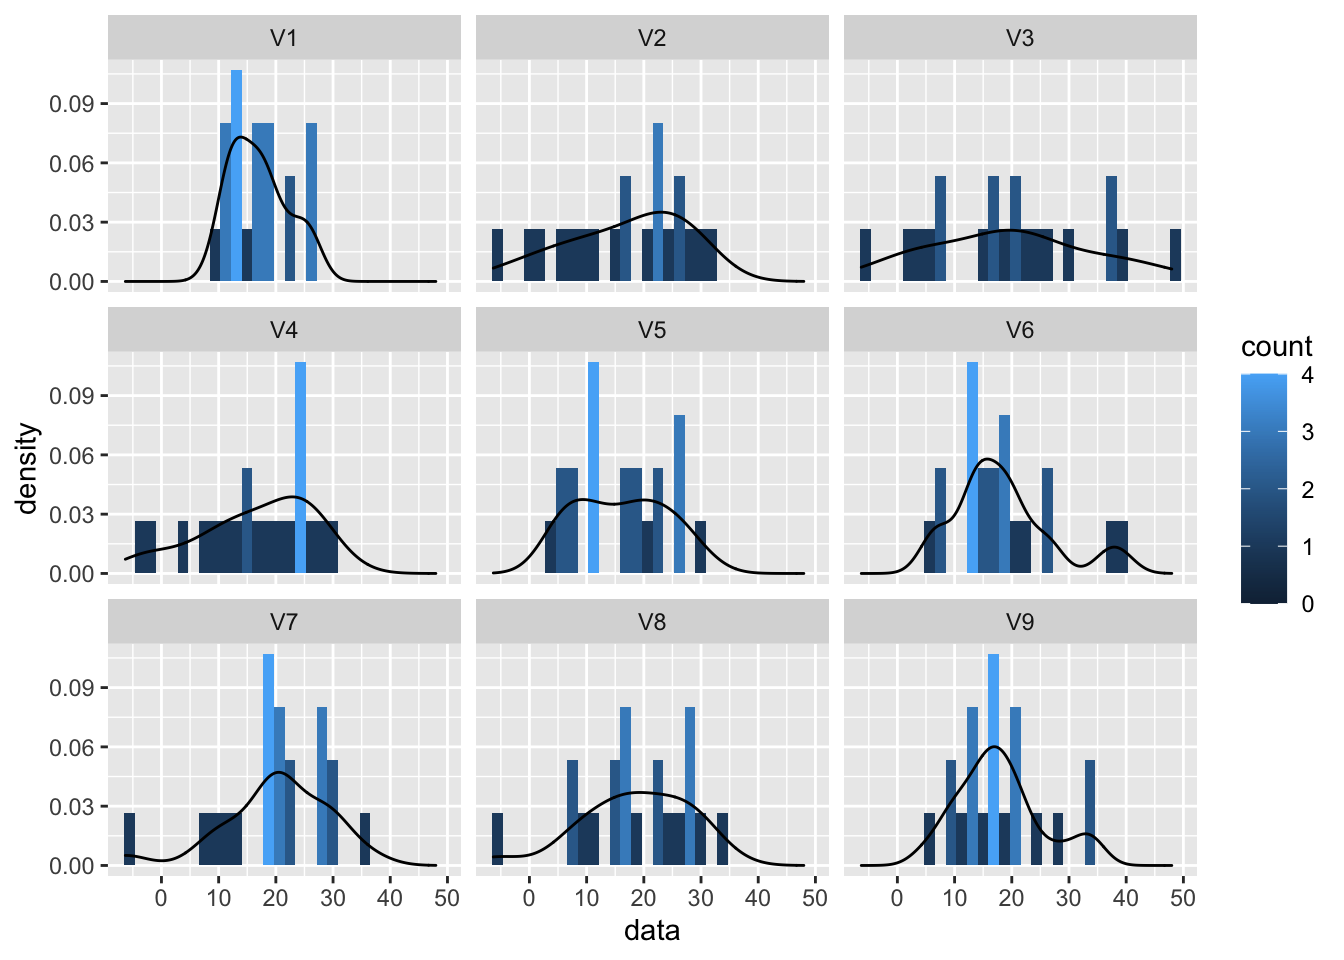
\includegraphics{Statistiek_2020_2021_files/figure-latex/unnamed-chunk-105-1.pdf}

Gezien er vrij weinig data punten zijn en omdat er veel distributies vergeleken moeten worden is het handiger om dit via een boxplot te doen.

\begin{Shaded}
\begin{Highlighting}[]
\NormalTok{normSim }\OperatorTok{\%\textgreater{}\%}\StringTok{ }\KeywordTok{gather}\NormalTok{(samp, data) }\OperatorTok{\%\textgreater{}\%}\StringTok{ }\KeywordTok{ggplot}\NormalTok{(}\KeywordTok{aes}\NormalTok{(}\DataTypeTok{x =}\NormalTok{ samp, }
    \DataTypeTok{y =}\NormalTok{ data)) }\OperatorTok{+}\StringTok{ }\KeywordTok{geom\_boxplot}\NormalTok{(}\DataTypeTok{outlier.shape =} \OtherTok{NA}\NormalTok{) }\OperatorTok{+}\StringTok{ }
\StringTok{    }\KeywordTok{geom\_point}\NormalTok{(}\DataTypeTok{position =} \StringTok{"jitter"}\NormalTok{)}
\end{Highlighting}
\end{Shaded}

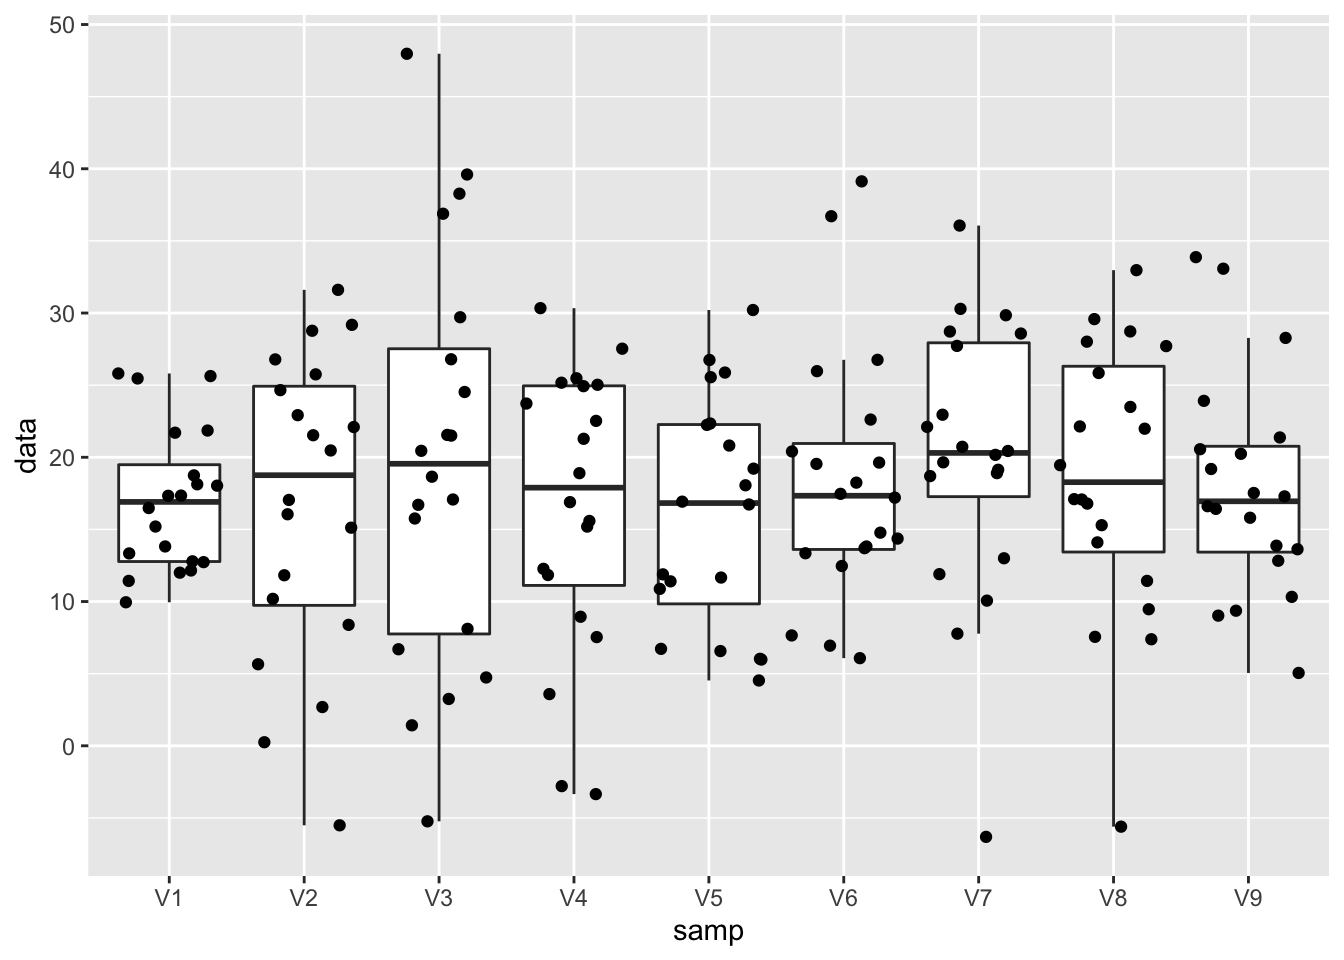
\includegraphics{Statistiek_2020_2021_files/figure-latex/unnamed-chunk-106-1.pdf}

Hoewel alle observaties in alle steekproeven uit dezelfde populatie zijn getrokken zien we toch vrij grote fluctuaties van steekproef tot steekproef in de mediaan, maar zeker ook in de boxgrootte en het bereik van de data in elke steekproef. Dus ondanks het feit dat we over een vrij grote steekproef beschikken (20 observaties) is er toch een grote variabiliteit van steekproef tot steekproef.

We gaan nu normaliteit na via QQ-plot.

\begin{enumerate}
\def\labelenumi{\arabic{enumi}.}
\tightlist
\item
  Zet data om in tidy data
\item
  maak een ggplot object
\item
  Voeg een laag toe met de QQ-plot via de functie \texttt{geom\_qq}
\item
  Voeg een laag toe met de rechte in de QQ-plot via de functie \texttt{geom\_qq\_line} om te kunnen evalueren hoe goed de data een normale verdeling volgt.
\end{enumerate}

\begin{Shaded}
\begin{Highlighting}[]
\NormalTok{normSim }\OperatorTok{\%\textgreater{}\%}\StringTok{ }\KeywordTok{gather}\NormalTok{(samp, data) }\OperatorTok{\%\textgreater{}\%}\StringTok{ }\KeywordTok{ggplot}\NormalTok{(}\KeywordTok{aes}\NormalTok{(}\DataTypeTok{sample =}\NormalTok{ data)) }\OperatorTok{+}\StringTok{ }
\StringTok{    }\KeywordTok{geom\_qq}\NormalTok{() }\OperatorTok{+}\StringTok{ }\KeywordTok{geom\_qq\_line}\NormalTok{() }\OperatorTok{+}\StringTok{ }\KeywordTok{facet\_wrap}\NormalTok{(}\OperatorTok{\textasciitilde{}}\NormalTok{samp)}
\end{Highlighting}
\end{Shaded}

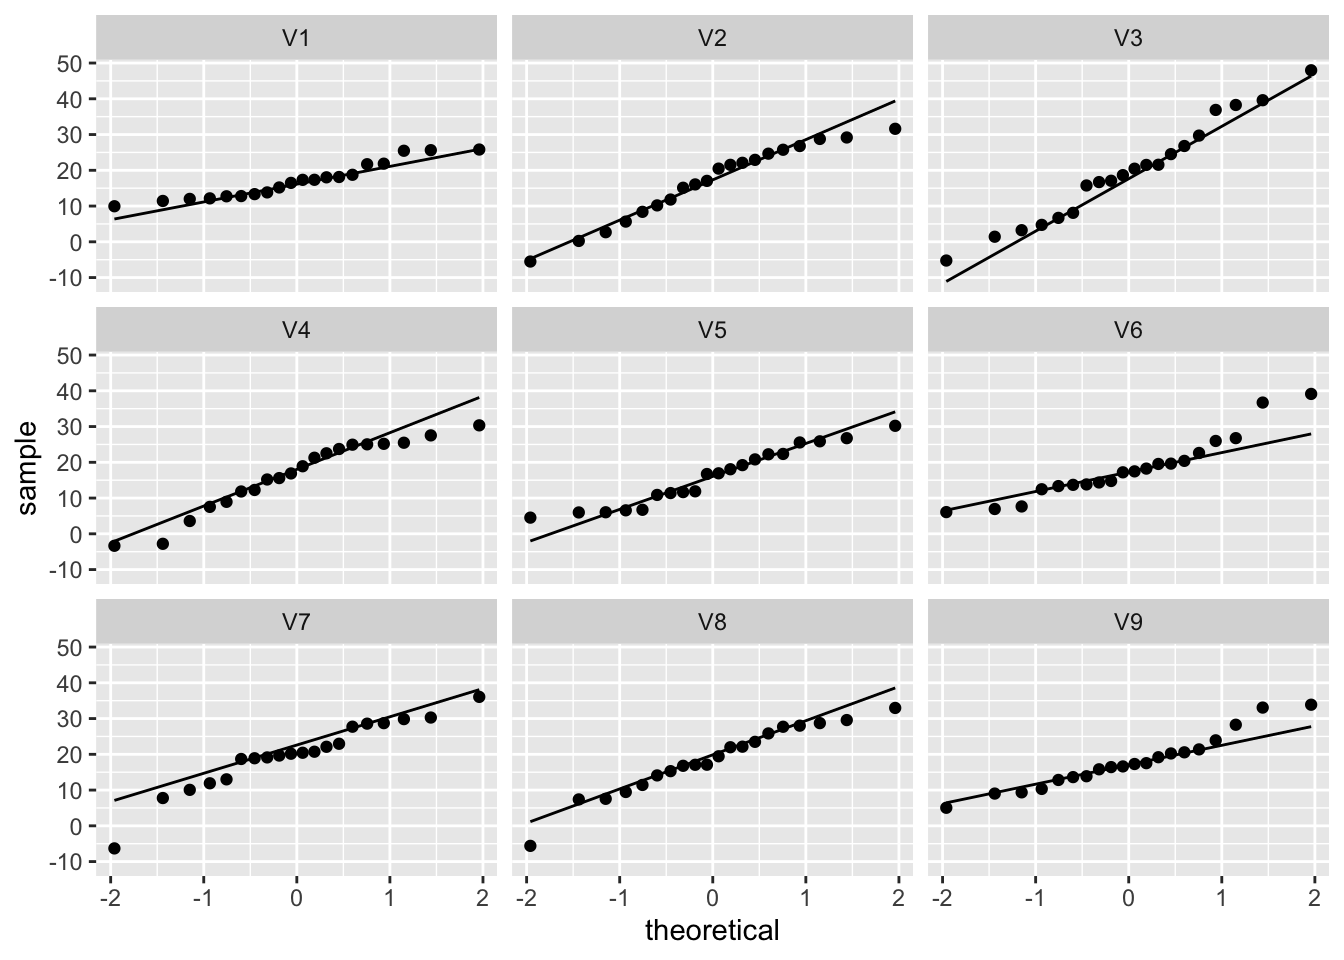
\includegraphics{Statistiek_2020_2021_files/figure-latex/unnamed-chunk-107-1.pdf}

Zelf voor Normal data zien we duidelijk nog afwijkingen door sampling variabiliteit! De plots laten ons toe om ons visueel te trainen om QQ-plots van Normale data te herkennen.

Om de interpretatie van de QQ-plot goed te kunnen illustreren gaan we een histogram en QQ-plot naast elkaar zetten.
D.m.v. het package \texttt{gridExtra} kunnen we meerdere GG-plot objecten in een matrix op dezelfde plot afbeelden.

\begin{enumerate}
\def\labelenumi{\arabic{enumi}.}
\tightlist
\item
  We maken een eerste object aan met het histogram. We slaan dit nu op als object p1 in plaats van dit te visualiseren.
\item
  Maak een object p2 met de QQ-plot
\item
  Gebruik de functie \texttt{grid.arrange} om de objecten p1 en p2 af te beelden en we geven aan dat we dit in 2 kolommen zullen doen \texttt{ncol=2}. (je kan ook de dimensie in rijen geven (nrow=1))
\end{enumerate}

\begin{Shaded}
\begin{Highlighting}[]
\KeywordTok{library}\NormalTok{(gridExtra)}
\NormalTok{p1 \textless{}{-}}\StringTok{ }\NormalTok{NHANES }\OperatorTok{\%\textgreater{}\%}\StringTok{ }\KeywordTok{filter}\NormalTok{(Gender }\OperatorTok{==}\StringTok{ "female"} \OperatorTok{\&}\StringTok{ }\OperatorTok{!}\KeywordTok{is.na}\NormalTok{(BMI)) }\OperatorTok{\%\textgreater{}\%}\StringTok{ }
\StringTok{    }\KeywordTok{ggplot}\NormalTok{(}\KeywordTok{aes}\NormalTok{(}\DataTypeTok{x =}\NormalTok{ BMI)) }\OperatorTok{+}\StringTok{ }\KeywordTok{geom\_histogram}\NormalTok{(}\KeywordTok{aes}\NormalTok{(}\DataTypeTok{y =}\NormalTok{ ..density.., }
    \DataTypeTok{fill =}\NormalTok{ ..count..)) }\OperatorTok{+}\StringTok{ }\KeywordTok{xlab}\NormalTok{(}\StringTok{"BMI"}\NormalTok{) }\OperatorTok{+}\StringTok{ }\KeywordTok{ggtitle}\NormalTok{(}\StringTok{"All females in study"}\NormalTok{) }\OperatorTok{+}\StringTok{ }
\StringTok{    }\KeywordTok{geom\_density}\NormalTok{(}\KeywordTok{aes}\NormalTok{(}\DataTypeTok{y =}\NormalTok{ ..density..))}

\NormalTok{p2 \textless{}{-}}\StringTok{ }\NormalTok{NHANES }\OperatorTok{\%\textgreater{}\%}\StringTok{ }\KeywordTok{filter}\NormalTok{(Gender }\OperatorTok{==}\StringTok{ "female"} \OperatorTok{\&}\StringTok{ }\OperatorTok{!}\KeywordTok{is.na}\NormalTok{(BMI)) }\OperatorTok{\%\textgreater{}\%}\StringTok{ }
\StringTok{    }\KeywordTok{ggplot}\NormalTok{(}\KeywordTok{aes}\NormalTok{(}\DataTypeTok{sample =}\NormalTok{ BMI)) }\OperatorTok{+}\StringTok{ }\KeywordTok{geom\_qq}\NormalTok{() }\OperatorTok{+}\StringTok{ }\KeywordTok{geom\_qq\_line}\NormalTok{()}

\KeywordTok{grid.arrange}\NormalTok{(p1, p2, }\DataTypeTok{ncol =} \DecValTok{2}\NormalTok{)}
\end{Highlighting}
\end{Shaded}

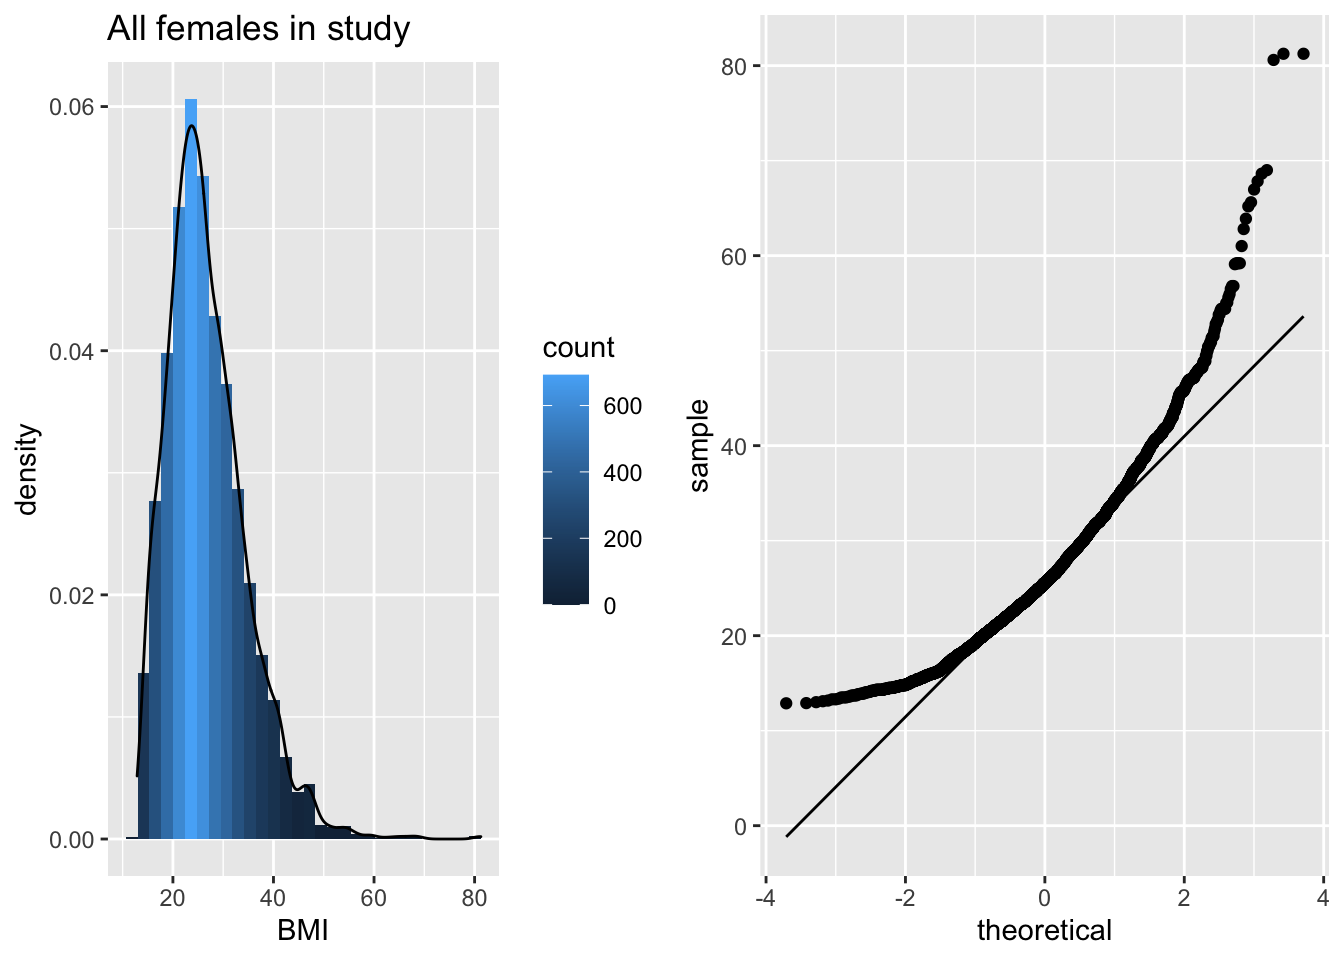
\includegraphics{Statistiek_2020_2021_files/figure-latex/unnamed-chunk-108-1.pdf}

The QQ-plot toont dat de kwantielen van de data in de steekproef

\begin{itemize}
\item
  groter zijn (boven de lijn liggen) dan wat we verwachten voor Normaal verdeelde data in de linkerstaart: compressie van de linkerstaart t.o.v. de Normale verdeling. De waarden in de linkerstaart liggen dus dichter bij top van de distributie dan wat we verwachten voor normaal verdeelde data.
\item
  groter zijn (boven de lijn liggen) dan wat we verwachten voor Normaal verdeelde data: lange staart naar rechts. De waarden in de rechterstaart liggen dus verder van de top van de distributie dan wat we verwachten voor normaal verdeelde data.
\end{itemize}

We zien dus duidelijk dat de data scheef verdeeld zijn naar rechts.

\hypertarget{sec:explCatVar}{%
\section{Samenvattingsmaten voor categorische variabelen}\label{sec:explCatVar}}

De samenvattingsmaten uit de vorige sectie (gemiddelde, mediaan, standaarddeviatie, \ldots) kunnen niet zomaar toegepast worden voor de beschrijving van categorische variabelen. In deze sectie gaan we hier dieper op in, daarbij onderscheid makend tussen enerzijds gegevens die uit prospectieve studies of lukrake steekproeven afkomstig zijn, en anderzijds gegevens uit retrospectieve studies.

\hypertarget{prospectieve-studies-en-lukrake-steekproeven}{%
\subsection{Prospectieve studies en lukrake steekproeven}\label{prospectieve-studies-en-lukrake-steekproeven}}

\begin{example}[Houtluizen]
\protect\hypertarget{exm:unnamed-chunk-109}{}{\label{exm:unnamed-chunk-109} \iffalse (Houtluizen) \fi{} }
\end{example}

Een bioloog verzamelt `s nachts bladerafval op een lukrake plaats van 1 m\(^2\)
in 2 wouden, waarvan 1 met klei- en 1 met kalkgrond. Op elke plaats telt hij het aantal houtluizen van de species
Armadilidium of Oniscus, met als doel na te gaan of de ene soort vaker voorkomt op kleigrond dan op
kalkgrond\footnote{Merk op dat dit design niet optimaal is omdat replicaties op de verkeerde schaal werden bekomen. Idealiter moesten meer dan 2 stukken grond in de studie opgenomen worden omdat de 2 gekozen stukken grond in veel meer kunnen verschillen dan alleen het bodemtype. Verschillen in de verdeling van houtluizen kunnen bijgevolg niet zomaar aan het bodemtype kunnen toegeschreven worden.}. Tabel \ref{tab:cox} toont de bekomen gegevens. Hier stelt \(a\) (\(c\)) het aantal houtluizen van de soort Armadilidium (Oniscus) voor op kleigrond, en \(b\) (\(d\)) het aantal houtluizen van de soort Armadilidium (Oniscus) op kalkgrond.

\begin{table}

\caption{\label{tab:cox}Kruistabel van species houtluis versus type grond.}
\centering
\begin{tabular}[t]{llll}
\toprule
  & Armadil. & Oniscus & Totaal\\
\midrule
Klei & 14 (a) & 6 (c) & 20 (a+c)\\
Kalk & 22 (b) & 46 (d) & 68 (b+d)\\
Totaal & 36 (a+b) & 52 (c+d) & 88 (n)\\
\bottomrule
\end{tabular}
\end{table}

\textbf{Einde voorbeeld}

Er zijn verschillende manieren om de resultaten van deze studie te
beschrijven. De kans dat 1 van beide species houtluizen van de soort Armadilidium is, is \(p_{kl}=a/(a+c)=0.70\) of 70\% op kleigrond en \(p_{ka}=b/(b+d)=0.32\) of 32\% op kalkgrond.

\begin{definition}[absolute risico verschil]
\protect\hypertarget{def:unnamed-chunk-110}{}{\label{def:unnamed-chunk-110} \iffalse (absolute risico verschil) \fi{} }
\end{definition}
Het \textbf{absolute risico verschil} of absolute kansverschil op een gegeven gebeurtenis (bvb. om Armadilidium aan te treffen) voor populatie T (Test, bvb. kleigrond) versus C (Controle, bvb. kalkgrond) wordt
met ARV genoteerd en gedefinieerd als het verschil

\begin{equation*}
ARV=p_T-p_C
\end{equation*}

tussen de kansen dat deze gebeurtenis zich voordoet in populaties T en C.

\textbf{Einde definitie}

Het ARV op Armadilidium tussen klei- en kalkgrond bedraagt 0.38, hetgeen suggereert dat de kans dat 1 van beide species houtluizen van de soort Armadilidium is, 38\% hoger is op kleigrond dan op kalkgrond. Een absoluut kansverschil
van 0 drukt uit dat de overeenkomstige kansen even groot zijn in beide
populaties en dat beide populaties dus vergelijkbaar zijn in termen van de bestudeerde uitkomst.

Het absolute kansverschil zegt echter niet alles omtrent het
bestudeerde effect. Een kansverschil kan immers een grotere impact hebben
alnaargelang beide proporties \(p_T\) en \(p_C\) dicht bij 0 of 1 liggen, dan
wanneer ze in de buurt van 0.5 liggen.
Bijvoorbeeld, wanneer we de proportie
vrouwen jonger dan 60 jaar meten die borstkanker ontwikkelen, is
een risicoverschil tussen \(p_A=0.01\) voor vrouwen die het allel Leu/Leu bezitten op het BRCA1 gen
en \(p_B=0.001\) voor de overige vrouwen, wellicht belangrijker dan een verschil tussen \(p_C=0.41\) en \(p_D=0.401\) voor beide populaties. Een uitspraak dat het risico 0.9\% lager is in de ene dan in de andere populatie geeft om die reden slechts een beperkt beeld van het belang van die reductie. Een goede vergelijking van risico's, kansen of percentages moet om die reden ook rekening houden met het basisrisico (d.w.z. de kans op de bestudeerde uitkomst in een referentiepopulatie). Het ARV doet dit niet, in tegenstelling tot volgende associatiemaat.

\begin{definition}[relatief risico]
\protect\hypertarget{def:unnamed-chunk-111}{}{\label{def:unnamed-chunk-111} \iffalse (relatief risico) \fi{} }
\end{definition}
Het \textbf{relatief risico} op een gegeven gebeurtenis (bvb. om Armadilidium aan te treffen) voor populatie T (Test, bvb. kleigrond) versus C (Controle, bvb. kalkgrond) wordt met RR
genoteerd en gedefinieerd als het quotiënt

\begin{equation*}
RR=\frac{p_T}{p_C}
\end{equation*}

van de kansen dat deze gebeurtenis zich voordoet in populaties T en C.

\textbf{Einde definitie}

In de studie naar houtluizen bedraagt dit \(RR=0.70/0.32=2.2\). Dit
suggereert dat er 2.2 keer zoveel kans om een houtluis van de soort Armadilidium (i.p.v. Oniscus) aan te treffen op kleigrond dan op kalkgrond. Een
relatief risico van 1 drukt uit dat beide populaties dus vergelijkbaar zijn in termen van de bestudeerde uitkomst.

Een nadeel van het relatief risico is dat ze, in tegenstelling tot het absolute risico verschil, niet goed duidelijk maakt hoeveel meer individuen de bestudeerde uitkomst ondervinden in de ene dan in de andere populatie. Bijvoorbeeld, zelfs wetende dat het relatief risico op Armidilidium in klei-versus kalkgrond 2.2 bedraagt, is het niet mogelijk om uit te maken hoeveel meer houtluizen van de soort Armidilidium zich manifesteren op kleigrond. Als de kans om Armidilidium aan te treffen i.p.v. Oniscus 0.1\% bedraagt op kalkgrond, dan verwacht men dat er per 10000 houtluizen (van de soort Armidilidium of Oniscus) er 10 van de soort Armidilidium zullen zijn op kalkgrond en 22 op kleigrond, wat neerkomt op een verwaarloosbaar verschil van 12. Als de kans om Armidilidium aan te treffen i.p.v. Oniscus 40\% bedraagt op kalkgrond, dan verwacht men dat er per 10000 houtluizen (van de soort Armidilidium of Oniscus) er 4000 van de soort Armidilidium zullen zijn op kalkgrond en 8800 op kleigrond, wat neerkomt op een aanzienlijk verschil van 4800. Soms rapporteert men in de plaats van het relatief risico, het
\emph{relatieve risico verschil} \(ARV/p_C=RR-1\). Voor de gegeven studie
bedraagt dit 1.2. Het drukt uit dat de toename (van kalk- naar kleigrond) in kans om Armadilidium aan te treffen succes meer dan 1 keer zo groot is als het basisrisico in de controlegroep (kalkgrond).

Merk op dat alle bovenstaande associatiematen eveneens gebruikt kunnen
worden wanneer men, in tegenstelling tot wat in een prospectieve studie
gebeurt, een volledig lukrake groep proefpersonen selecteert zonder vast te
leggen hoeveel van hen al dan niet blootgesteld zijn.

\hypertarget{subsec:retrospect}{%
\subsection{Retrospectieve studies}\label{subsec:retrospect}}

Beschouw de case-controle studie uit Voorbeeld \ref{exm:brcaLeu}, waarvan
de gegevens samengevat zijn in Tabel \ref{tab:leu2}. Omdat men in
zo'n design op zoek gaat naar \(a+b+c\) lukraak gekozen controles en \(d+e+f\) lukraak
gekozen cases, liggen de marges \(a+b+c\) en \(d+e+f\) vast en is het bijgevolg
onmogelijk om het risico op case (bvb. risico op borstkanker) te schatten. Dit is noch mogelijk binnen de
totale groep, noch binnen de groep van blootgestelden (d.i. vrouwen met allel Leu/Leu), noch binnen de groep
niet-blootgestelden. Immers, de kans op case binnen die geobserveerde groep reflecteert hoofdzakelijk de verhouding waarin cases en controles in totaal werden gekozen door het design. Alleen analyses die de kolomtotalen
in de tabel vast gegeven veronderstellen, zijn hier zinvol. Dit heeft tot
gevolg dat \emph{het relatief risico} op de aandoening (d.w.z. op \emph{case})
in de populatie voor blootgestelden versus niet-blootgestelden niet
rechtstreeks kan geschat worden op basis van gegevens uit een \emph{case-controle studie}. Analoog kan ook het bijhorende \emph{absolute risicoverschil niet geschat} worden.

\begin{table}

\caption{\label{tab:leu2}Kruistabel van borstkanker-status versus BRCA1-allel.}
\centering
\begin{tabular}[t]{llll}
\toprule
Genotype & Controles & Cases & Totaal\\
\midrule
Pro/Pro & 266 (a) & 342 (d) & 608 (a+d)\\
Pro/Leu & 250 (b) & 369 (e) & 619 (b+e)\\
Leu/Leu & 56 (c) & 89 (f) & 145 (c+f)\\
Totaal & 572 (a+b+c) & 800 (d+e+f) & 1372 (n)\\
\bottomrule
\end{tabular}
\end{table}

Wel heeft men informatie over de kans om het allel Leu/Leu aan te treffen bij cases, \(\pi_1=f/(d+e+f)=89/800=11.1\%\), en de kans op het allel Leu/Leu bij controles, \(\pi_0=c/(a+b+c)=56/572=9.8\%\). Het relatief risico op blootstelling voor cases versus
controles is bijgevolg \(11.1/9.8=1.14\). Vrouwen met borstkanker hebben dus
14\% meer kans om de allelcombinatie Leu/Leu te hebben op het BRCA1 gen dan vrouwen zonder borstkanker.
Dit suggereert dat er
een associatie\footnote{Al is het nog de vraag of die associatie toevallig is, dan wel systematisch. We komen in het hoofdstuk \ref{chap:categorisch}. terug op technieken om dit te onderzoeken.} is tussen het polymorfisme op het BRCA1 gen en borstkanker, maar drukt helaas niet uit hoeveel hoger het risico op borstkanker is voor vrouwen met de allelcombinatie Leu/Leu dan voor andere vrouwen. Om toch een antwoord te vinden op deze laatste vraag, voeren we een nieuwe risicomaat in.

\begin{definition}[Odds]
\protect\hypertarget{def:unnamed-chunk-112}{}{\label{def:unnamed-chunk-112} \iffalse (Odds) \fi{} }
\end{definition}
De \emph{odds} op een gebeurtenis wordt gedefinieerd als

\begin{equation*}
\frac{p}{1-p}
\end{equation*}

waarbij \(p\) de kans is op die gebeurtenis.

\textbf{Einde definitie}

De odds is dus een transformatie van het risico, met onder andere de
volgende eigenschappen:

\begin{itemize}
\item
  de odds neemt waarden aan tussen nul en oneindig.
\item
  de odds is gelijk aan 1 als en slechts als de kans zelf gelijk is aan
  1/2.
\item
  de odds neemt toe als de kans toeneemt.
\end{itemize}

Het gebruik van odds is populair onder gokkers omdat het uitdrukt hoeveel
waarschijnlijker het is om te winnen dan om te verliezen. Een odds op winnen
gelijk aan 1 drukt bijvoorbeeld uit dat het even waarschijnlijk is om te
winnen dan om te verliezen. Een odds op winnen gelijk aan 0.9 drukt uit men
per 10 verliesbeurten, 9 keer verwacht te winnen. In de genetische associatiestudie uit Voorbeeld \ref{exm:brcaLeu}
is de odds op allel Leu/Leu bij cases gelijk aan
\(\mbox{odds}_1=f/(d+e)=89/711=0.125\) en bij controles gelijk aan \(\mbox{odds}_2=c/(a+b)=56/516=0.109\). Vrouwen met borstkanker hebben bijgevolg ongeveer 8 (\(\approx 1/0.125\)) keer meer kans om de allelcombinatie Leu/Leu niet te hebben op het BRCA1 gen dan om het wel te hebben.
Om de associatie tussen blootstelling
en uitkomst te beschrijven, kan men nu een verhouding van odds (odds ratio)
gebruiken in plaats van een verhouding van risico's (relatief risico).

\begin{definition}[Odds ratio]
\protect\hypertarget{def:unnamed-chunk-113}{}{\label{def:unnamed-chunk-113} \iffalse (Odds ratio) \fi{} }
\end{definition}
De \textbf{odds ratio} op een gegeven gebeurtenis (bvb. borstkanker) voor populatie T (bvb. vrouwen met allel Leu/Leu) versus C (bvb. vrouwen zonder allel Leu/Leu) wordt met OR genoteerd en gedefinieerd als het quotiënt
\begin{equation*}
OR=\frac{\mbox{odds}_T}{\mbox{odds}_C}
\end{equation*}
van de odds op deze gebeurtenis in populaties T en C.

\textbf{Einde definitie}

Op basis van de gegevens in Tabel \ref{tab:leu2} kan de odds ratio op
blootstelling voor cases versus controles geschat worden d.m.v. het kruisproduct

\begin{equation*}
\frac{ \frac{ f/(d+e+f)}{(d+e)/(d+e+f)} }{ \frac{c/(a+b+c)}{(a+b)/(a+b+c)}} = \frac{f(a+b)}{c (d+e)}
\end{equation*}

In het bijzonder vinden we dat de odds op allelcombinatie Leu/Leu voor vrouwen met versus zonder borstkanker gelijk is aan \(OR=(89\times 516)/(56\times 711)=1.15\). Helaas drukt dit resultaat nog steeds
niet uit hoeveel meer risico op borstkanker vrouwen met de allelcombinatie Leu/Leu lopen.

Was de bovenstaande studie echter een volledig lukrake steekproef geweest
(waarbij het aantal cases en controles niet per design werden vastgelegd),
dan konden we daar ook de odds ratio op borstkanker berekenen voor mensen
met versus zonder het allel Leu/leu. We zouden dan vaststellen dat dit gelijk is
aan

\begin{equation*}
\frac{ \frac{ f/(c+f)}{c/(c+f)} }{ \frac{(d+e)/(a+b+d+e)}{(a+b)/(a+b+d+e)}} = \frac{f(a+b)}{c(d+e)},
\end{equation*}

en bijgevolg dezelfde waarde aanneemt. Dat is omdat de odds ratio een
\emph{symmetrische associatiemaat} is zodat de odds ratio op `case' voor
blootgestelden versus niet-blootgestelden steeds gelijk is aan de odds op
blootstelling voor cases versus controles. Hieruit volgt dat voor het
schatten van de odds ratio het er niet toe doet of we prospectief werken
zoals in een typische cohort studie, of retrospectief zoals in een typische
case-controle studie. In het bijzonder kunnen we in de genetische associatiestudie uit
Voorbeeld \ref{exm:brcaLeu} de odds op borstkanker voor vrouwen met allel Leu/leu
versus zonder berekenen als \(OR=89\times 516/(56\times 711)=1.15\).
De odds op borstkanker is bijgevolg 15\% hoger bij vrouwen met die specifieke allelcombinatie.

Stel nu dat we met \(p_T\) en \(p_C\) respectievelijk de kans op case noteren
voor blootgestelden en niet-blootgestelden. Wanneer beide kansen klein zijn
(namelijk \(p_T<5\%\) en \(p_C<5\%\)), dan is de odds een goede benadering voor
het risico. Dit is omdat in dat geval \(\mbox{odds}_T=p_T/(1-p_T)\approx p_T\) en \(\mbox{odds}_C=p_C/(1-p_C)\approx p_C\). Er volgt dan bovendien dat de odds ratio
een goede benadering voor het relatief risico:

\begin{equation*}
OR=\frac{\mbox{ odds}_T}{\mbox{
odds}_C}\approx \frac{p_T}{p_C}=RR
\end{equation*}

Wetende dat het risico op borstkanker laag is, mogen we
op basis van de gevonden OR van 1.15 bijgevolg
besluiten dat het risico (i.p.v. de odds) op borstkanker (bij benadering) 15\% hoger ligt bij vrouwen met het allel Leu/Leu op het BRCA1 gen. Dit is een bijzonder
nuttige eigenschap omdat (a) het relatief risico, dat niet rechtstreeks
geschat kan worden in case-controle studies, gemakkelijker te interpreteren
is dan de odds ratio; en (b) de odds ratio bepaalde wiskundige eigenschappen
heeft die ze aantrekkelijker maakt dan een relatief risico in statistische
modellen\footnote{Dit is bijvoorbeeld het geval in logistische regressiemodellen die gebruikt worden om het
  risico op een bepaalde aandoening te modelleren in functie van prognostische
  factoren.}. Algemeen is de odds ratio echter steeds verder van 1 verwijderd
dan het relatief risico. Wetende dat de odds ratio op borstkanker 1.15
bedraagt voor vrouwen met versus zonder de allelcombinatie Leu/Leu, kunnen we bijgevolg meer
nauwkeurig besluiten dat het overeenkomstige relatief risico tussen 1 en 1.15
gelegen is (maar niettemin dicht bij 1.15).

Omdat de odds ratio moeilijker te interpreteren is dan een relatief risico
en bijgevolg misleidend kan zijn, valt deze laatste steeds te verkiezen in
situaties (zoals prospectieve studies) waar het mogelijk is om het relatief
risico in de populatie te schatten. In sommige case-controle studies (nl.
matched case-controle studies) wordt voor elke case een controle gezocht die
bepaalde karakteristieken gemeenschappelijk heeft, teneinde een betere
onderlinge vergelijkbaarheid te garanderen. In dat geval moet de
statistische analyse (inclusief de manier om odds ratio's te schatten)
rekening houden met het feit dat de resultaten van elke case gecorreleerd of
verwant zijn met de resultaten van de bijhorende controle.

\hypertarget{rates-versus-risicos}{%
\subsection{Rates versus risico's}\label{rates-versus-risicos}}

Vaak wordt het begrip \emph{risico} verward met het begrip \emph{rate}. Een
\emph{rate} drukt een aantal gebeurtenissen (bvb. aantal sterfte- of
ziektegevallen) uit per eenheid in de populatie in een bepaalde tijdspanne.
Bijvoorbeeld, een \emph{crude mortality rate (CMR)} voor een bepaald
jaartal is gedefinieerd als 1000 maal het aantal sterftegevallen dat
optreedt in dat jaar gedeeld door de grootte van de beschouwde populatie
halfweg dat jaar. De reden dat met 1000 wordt vermenigvuldigd is dat het
bijvoorbeeld makkelijker na te denken is over een CMR van 12 sterftes per
1000 in Engeland en Wales, dan over 0.012 sterftes per individu. Indien een
specifieke leeftijdsgroep wordt gekozen, verkrijgt men de \emph{leeftijdsspecifieke mortality rate} als 1000 maal het aantal sterftegevallen
dat optreedt in een bepaald jaar en bepaalde leeftijdsgroep gedeeld door de
grootte van de beschouwde populatie in die leeftijdsklasse halfweg dat jaar.
In tegenstelling tot de incidentie, is de prevalentie geen rate omdat ze
niet een aantal gebeurtenissen uitdrukt over een zekere tijdspanne.

\hypertarget{associaties-tussen-twee-variabelen}{%
\section{Associaties tussen twee variabelen}\label{associaties-tussen-twee-variabelen}}

Tot nog toe zijn we hoofdzakelijk ingegaan op zogenaamde univariate beschrijvingen waarbij slechts 1 variabele onderzocht wordt. In de meeste wetenschappelijke studies wenst men echter associaties tussen 2 of meerdere variabelen te onderzoeken, bijvoorbeeld tussen een interventie en de daarop volgende respons. In deze Sectie onderzoeken we hoe associaties tussen 2 variabelen kunnen beschreven worden. We maken daarbij onderscheid naargelang het type van de variabelen.

\hypertarget{subsec:kruistabel}{%
\subsection{Associatie tussen twee kwalitatieve variabelen}\label{subsec:kruistabel}}

Als twee kwalitatieve variabelen niet veel verschillende waarden aannemen,
dan is een \emph{kruistabel} aangewezen om hun associatie voor te stellen.
In deze tabel worden de verschillende waarden die de ene variabele aanneemt
in de kolommen uitgezet en de verschillende waarden die de andere variabele
aanneemt in de rijen. In elke cel van de tabel (die overeenkomt met 1
specifieke combinatie van waarden voor beide variabelen) wordt de frequentie
neergeschreven.

\begin{table}

\caption{\label{tab:genderBMI}Kruistabel van Gender vs BMI klasse.}
\centering
\begin{tabular}[t]{lrrrr}
\toprule
  & 12.0\_18.5 & 18.5\_to\_24.9 & 25.0\_to\_29.9 & 30.0\_plus\\
\midrule
female & 629 & 1616 & 1179 & 1402\\
male & 648 & 1295 & 1485 & 1349\\
\bottomrule
\end{tabular}
\end{table}

Tabel \ref{tab:genderBMI} toont zo'n kruistabel voor het aantal mannen en vrouwen per BMI klasse. Dergelijke eenvoudige kruistabel met slechts 2 rijen en 4 kolommen, noemt men ook een \(2\times 4\) tabel.

\hypertarget{subsec:asskwalcont}{%
\subsection{Associatie tussen één kwalitatieve en één continue variabele}\label{subsec:asskwalcont}}

Boxplots zijn meer compact dan een histogram en laat om die reden gemakkelijker vergelijkingen tussen verschillende groepen toe. Twee dergelijke boxplots
worden getoond in Figuur \ref{fig:boxplotCholGender}.

\begin{Shaded}
\begin{Highlighting}[]
\NormalTok{NHANES }\OperatorTok{\%\textgreater{}\%}\StringTok{ }\KeywordTok{ggplot}\NormalTok{(}\KeywordTok{aes}\NormalTok{(}\DataTypeTok{x =}\NormalTok{ Gender, }\DataTypeTok{y =} \KeywordTok{log}\NormalTok{(DirectChol))) }\OperatorTok{+}\StringTok{ }
\StringTok{    }\KeywordTok{geom\_boxplot}\NormalTok{() }\OperatorTok{+}\StringTok{ }\KeywordTok{ylab}\NormalTok{(}\StringTok{"log(Direct Cholestorol)"}\NormalTok{)}
\end{Highlighting}
\end{Shaded}

\begin{figure}

{\centering 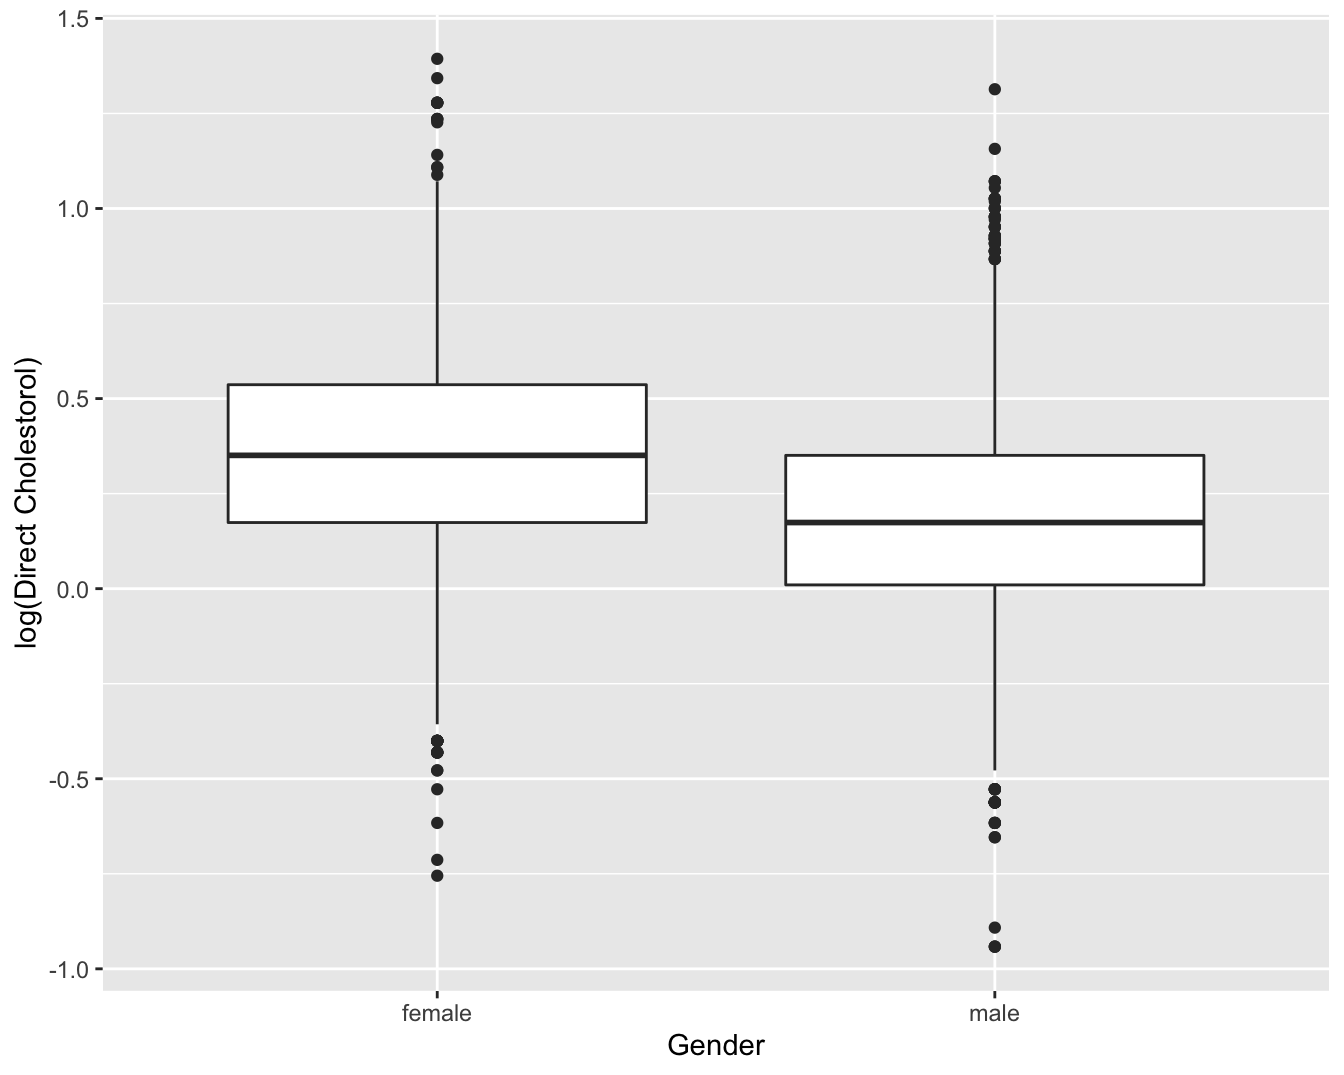
\includegraphics[width=1\linewidth]{Statistiek_2020_2021_files/figure-latex/boxplotCholGender-1} 

}

\caption{Boxplot van log-getransformeerde directe HDL cholestorol concentratie in functie van Gender voor alle subjecten van de NHANES studie.}\label{fig:boxplotCholGender}
\end{figure}

Op basis van deze figuur
stellen we vast dat hogere log-cholestorol concentraties
geobserveerd worden bij vrouwen dan bij mannen, maar dat de variabiliteit
van de log-concentraties vergelijkbaar is tussen de 2 groepen. De vraag blijft of we hier kunnen spreken van een systematisch hogere
log-cholestorol concentratie tussen vrouwen en mannen. We zullen in Hoofdstuk \ref{chap:besluit} dieper op deze vraag ingaan.

Figuur \ref{fig:boxplotCholGender} kan men samenvatten door gemiddelde verschillen tussen beide groepen te rapporteren. Hier stellen we een gemiddeld verschil van 0.17 in directe HDL cholestorol concentratie vast op de log schaal tussen vrouwen en mannen.
Gezien we weten dat \(\log(C_2)-\log(C_1)=\log(C_2/C_1)\) weten we dat de HDL cholestorol concentratie in de NHANES studie gemiddeld 1.19 keer hoger ligt voor vrouwen dan voor mannen.

In de introductie hebben we bij het microbiome voorbeeld gezien dat het ook erg nuttig is om de ruwe data weer te geven op de boxplot. Als het aantal gegevens niet te hoog is kunnen we eenvoudig een extra laag toevoegen met de originele datapunten. Merk op dat het wel belangrijk is om de outliers dan niet weer te geven in de boxplot, anders zal men deze twee keer afbeelden. Eens in de geom\_boxplot laag een eens in de geom\_point laag. Daarom zetten we het symbool voor de outliers op NA.

In onderstaande grafiek plotten we de relatieve abundanties van \textbf{Staphylococcus} van de oksel microbiome case study.

\begin{enumerate}
\def\labelenumi{\arabic{enumi}.}
\tightlist
\item
  We pipen het \texttt{ap} dataframe naar \texttt{ggplot}
\item
  We selecteren de data voor de plot via \texttt{ggplot(aes(x=trt,y=rel))}
\item
  We voegen laag toe voor de boxplot dmv de functie \texttt{geom\_boxplot()}. Merk op dat we het argument \texttt{outlier.shape} op NA (not available) zetten \texttt{outlier.shape=NA} in the \texttt{geom\_boxplot} functie omdat we anders outliers twee keer weer zullen geven. Eerst via de boxplot laag en daarna omdat we een laag met alle ruwe data toevoegen aan de plot.
\item
  We geven de ruwe data weer via de \texttt{geom\_point(position="jitter")} functie. We gebruiken hierbij het argument position=`jitter' zodat we wat random ruis toevoegen aan de x-cordinaat zodat de gegevens elkaar niet overlappen.
\end{enumerate}

\begin{Shaded}
\begin{Highlighting}[]
\NormalTok{ap \textless{}{-}}\StringTok{ }\KeywordTok{read\_csv}\NormalTok{(}\StringTok{"https://raw.githubusercontent.com/GTPB/PSLS20/master/data/armpit.csv"}\NormalTok{)}

\NormalTok{ap }\OperatorTok{\%\textgreater{}\%}\StringTok{ }\KeywordTok{ggplot}\NormalTok{(}\KeywordTok{aes}\NormalTok{(}\DataTypeTok{x =}\NormalTok{ trt, }\DataTypeTok{y =}\NormalTok{ rel)) }\OperatorTok{+}\StringTok{ }\KeywordTok{geom\_boxplot}\NormalTok{(}\DataTypeTok{outlier.shape =} \OtherTok{NA}\NormalTok{) }\OperatorTok{+}\StringTok{ }
\StringTok{    }\KeywordTok{geom\_point}\NormalTok{(}\DataTypeTok{position =} \StringTok{"jitter"}\NormalTok{)}
\end{Highlighting}
\end{Shaded}

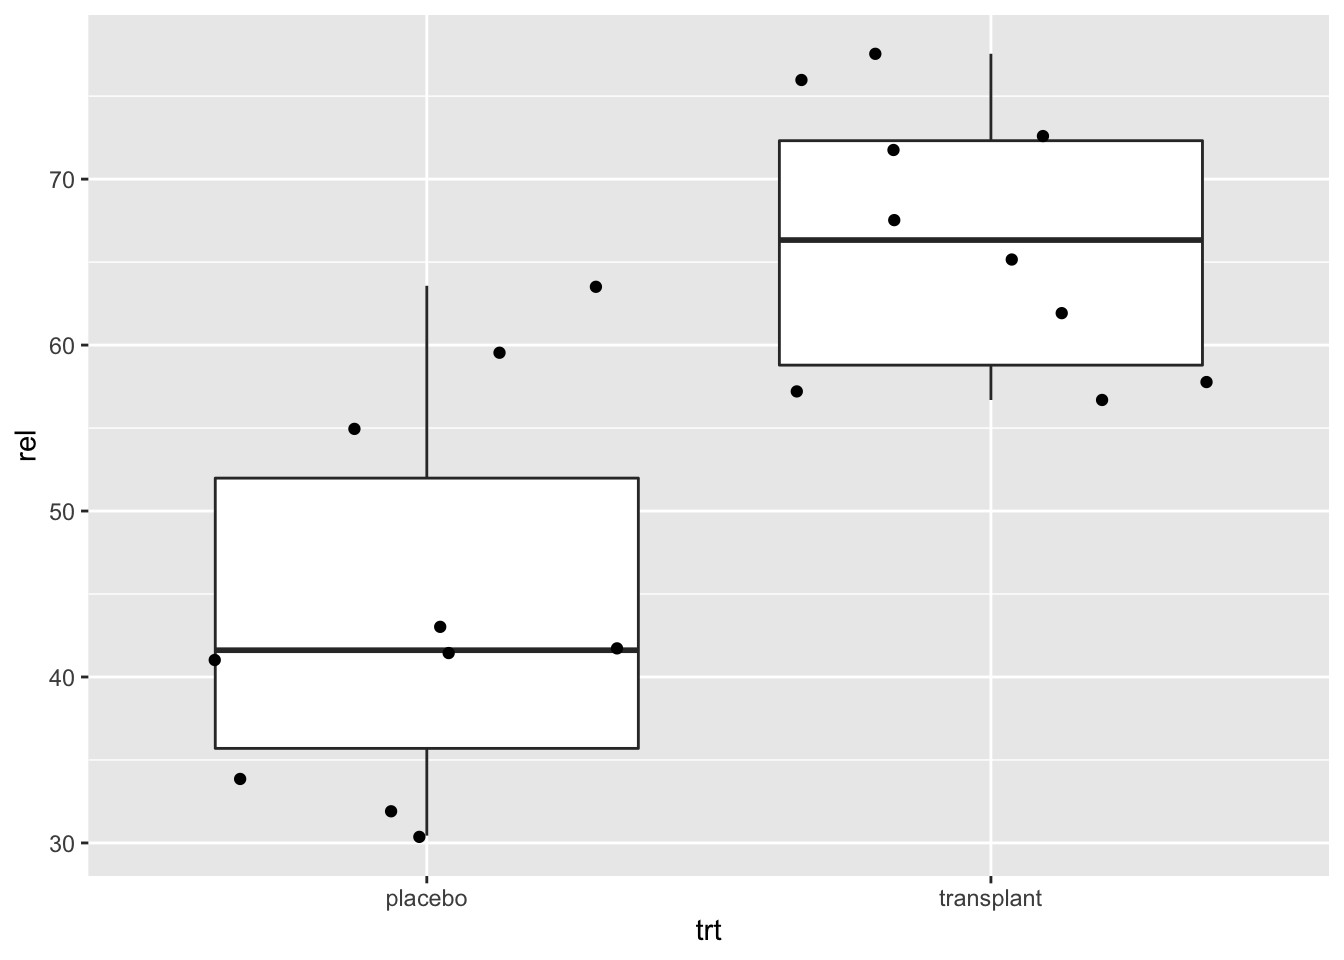
\includegraphics{Statistiek_2020_2021_files/figure-latex/unnamed-chunk-114-1.pdf}

Dot-plots zijn bijzonder interessant in pre-test post-test designs waar dezelfde subjecten op
verschillende tijdstippen worden geobserveerd. In dat geval kunnen de uitkomsten
uitgezet worden op de Y-as en de tijdstippen op de X-as, en kunnen de
metingen voor eenzelfde subject worden verbonden met een lijn.

Een
voorbeeld hiervan is weergegeven in Figuur \ref{fig:captoDot}. De figuur vat de gegevens samen van de captopril studie die de centrale dataset vormt van Hoofdstuk \ref{chap:besluit}. In de studie wenst men het effect van een bloeddrukverlagend geneesmiddel captopril evalueren. Voor elke patiënt in de studie werd de systolische bloeddruk twee keer gemeten: één keer voor en één keer na de behandeling met het bloeddruk verlagende medicijn captopril. In Figuur \ref{fig:captoDot} worden de metingen van dezelfde patiënt met een lijntje verbonden. Hierdoor krijgen we een heel duidelijk beeld van de gegevens. Namelijk, we krijgen een sterke indruk dat de bloeddruk daalt na het toedienen van captopril gezien we bijna voor alle patiënten een daling observeren.

\begin{Shaded}
\begin{Highlighting}[]
\CommentTok{\# Eerst lezen we de data in. Deze bevindt zich in}
\CommentTok{\# de subdirectory dataset Het is een tekstbestand}
\CommentTok{\# waarbij de kolommen van elkaar gescheiden zijn}
\CommentTok{\# d.m.v comma\textquotesingle{}s. sep=\textquotesingle{},\textquotesingle{} De eerste rij bevat de}
\CommentTok{\# namen van de variabelen}
\NormalTok{captopril \textless{}{-}}\StringTok{ }\KeywordTok{read.table}\NormalTok{(}\StringTok{"https://raw.githubusercontent.com/statOmics/sbc20/master/data/captopril.txt"}\NormalTok{, }
    \DataTypeTok{header =} \OtherTok{TRUE}\NormalTok{, }\DataTypeTok{sep =} \StringTok{","}\NormalTok{)}
\KeywordTok{head}\NormalTok{(captopril)}
\end{Highlighting}
\end{Shaded}

\begin{verbatim}
##   id SBPb DBPb SBPa DBPa
## 1  1  210  130  201  125
## 2  2  169  122  165  121
## 3  3  187  124  166  121
## 4  4  160  104  157  106
## 5  5  167  112  147  101
## 6  6  176  101  145   85
\end{verbatim}

\begin{Shaded}
\begin{Highlighting}[]
\NormalTok{captoprilTidy \textless{}{-}}\StringTok{ }\NormalTok{captopril }\OperatorTok{\%\textgreater{}\%}\StringTok{ }\KeywordTok{gather}\NormalTok{(type, bp, }\OperatorTok{{-}}\NormalTok{id)}

\NormalTok{captoprilTidy }\OperatorTok{\%\textgreater{}\%}\StringTok{ }\KeywordTok{filter}\NormalTok{(type }\OperatorTok{\%in\%}\StringTok{ }\KeywordTok{c}\NormalTok{(}\StringTok{"SBPa"}\NormalTok{, }\StringTok{"SBPb"}\NormalTok{)) }\OperatorTok{\%\textgreater{}\%}\StringTok{ }
\StringTok{    }\KeywordTok{mutate}\NormalTok{(}\DataTypeTok{type =} \KeywordTok{factor}\NormalTok{(type, }\DataTypeTok{levels =} \KeywordTok{c}\NormalTok{(}\StringTok{"SBPb"}\NormalTok{, }\StringTok{"SBPa"}\NormalTok{))) }\OperatorTok{\%\textgreater{}\%}\StringTok{ }
\StringTok{    }\KeywordTok{ggplot}\NormalTok{(}\KeywordTok{aes}\NormalTok{(}\DataTypeTok{x =}\NormalTok{ type, }\DataTypeTok{y =}\NormalTok{ bp)) }\OperatorTok{+}\StringTok{ }\KeywordTok{geom\_line}\NormalTok{(}\KeywordTok{aes}\NormalTok{(}\DataTypeTok{group =}\NormalTok{ id)) }\OperatorTok{+}\StringTok{ }
\StringTok{    }\KeywordTok{geom\_point}\NormalTok{()}
\end{Highlighting}
\end{Shaded}

\begin{figure}

{\centering 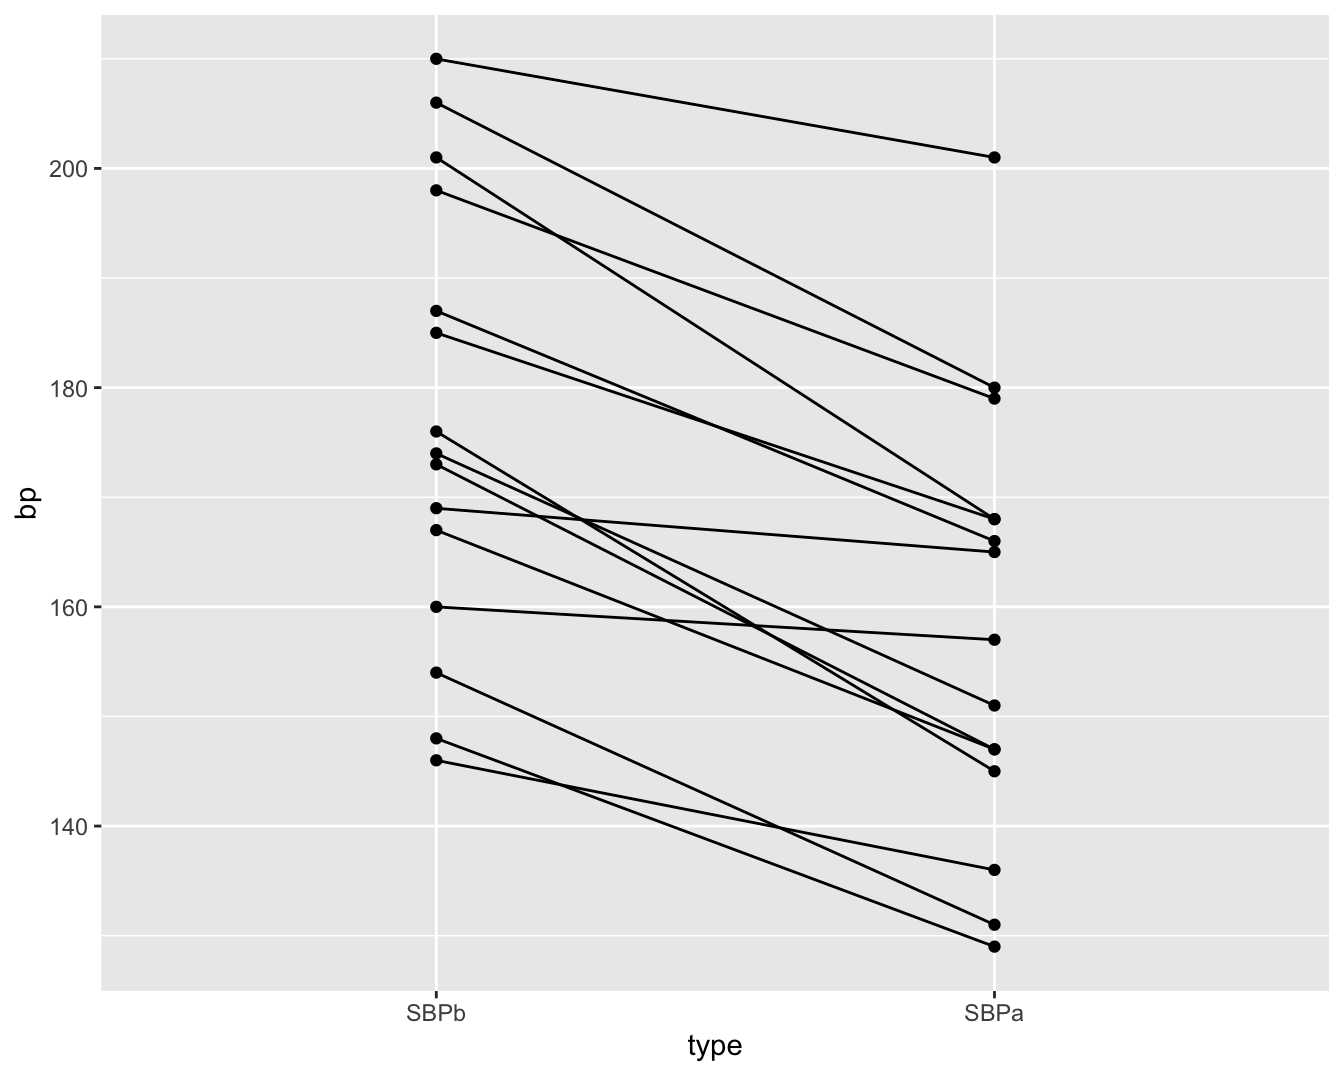
\includegraphics[width=1\linewidth]{Statistiek_2020_2021_files/figure-latex/captoDot-1} 

}

\caption{Dotplot van de systolische bloeddruk in de captopril studie voor en na het toedienen van het bloeddruk verlagend middel captopril.}\label{fig:captoDot}
\end{figure}

\hypertarget{sec:correlatie}{%
\section{Associatie tussen twee continue variabelen}\label{sec:correlatie}}

We zullen dit opnieuw illustreren aan de hand van de NHANES studie. We bestuderen hierbij lengte en gewicht bij vrouwen.

We voeren eerst een data exploratie uit waarbij we

\begin{enumerate}
\def\labelenumi{\arabic{enumi}.}
\tightlist
\item
  De volwassen vrouwen filteren uit de dataset
\item
  In het ggplot commando de lengte selecteren in de x-as en het gewicht in de y-as.
\item
  Een laag toevoegen d.m.v. \texttt{geom\_point} om een scatterplot te bekomen van y i.f.v. x.
\end{enumerate}

\begin{Shaded}
\begin{Highlighting}[]
\NormalTok{NHANES }\OperatorTok{\%\textgreater{}\%}\StringTok{ }\KeywordTok{filter}\NormalTok{(Age }\OperatorTok{\textgreater{}=}\StringTok{ }\DecValTok{18} \OperatorTok{\&}\StringTok{ }\NormalTok{Gender }\OperatorTok{==}\StringTok{ "female"}\NormalTok{) }\OperatorTok{\%\textgreater{}\%}\StringTok{ }
\StringTok{    }\KeywordTok{ggplot}\NormalTok{(}\KeywordTok{aes}\NormalTok{(}\DataTypeTok{x =}\NormalTok{ Height, }\DataTypeTok{y =}\NormalTok{ Weight)) }\OperatorTok{+}\StringTok{ }\KeywordTok{geom\_point}\NormalTok{()}
\end{Highlighting}
\end{Shaded}

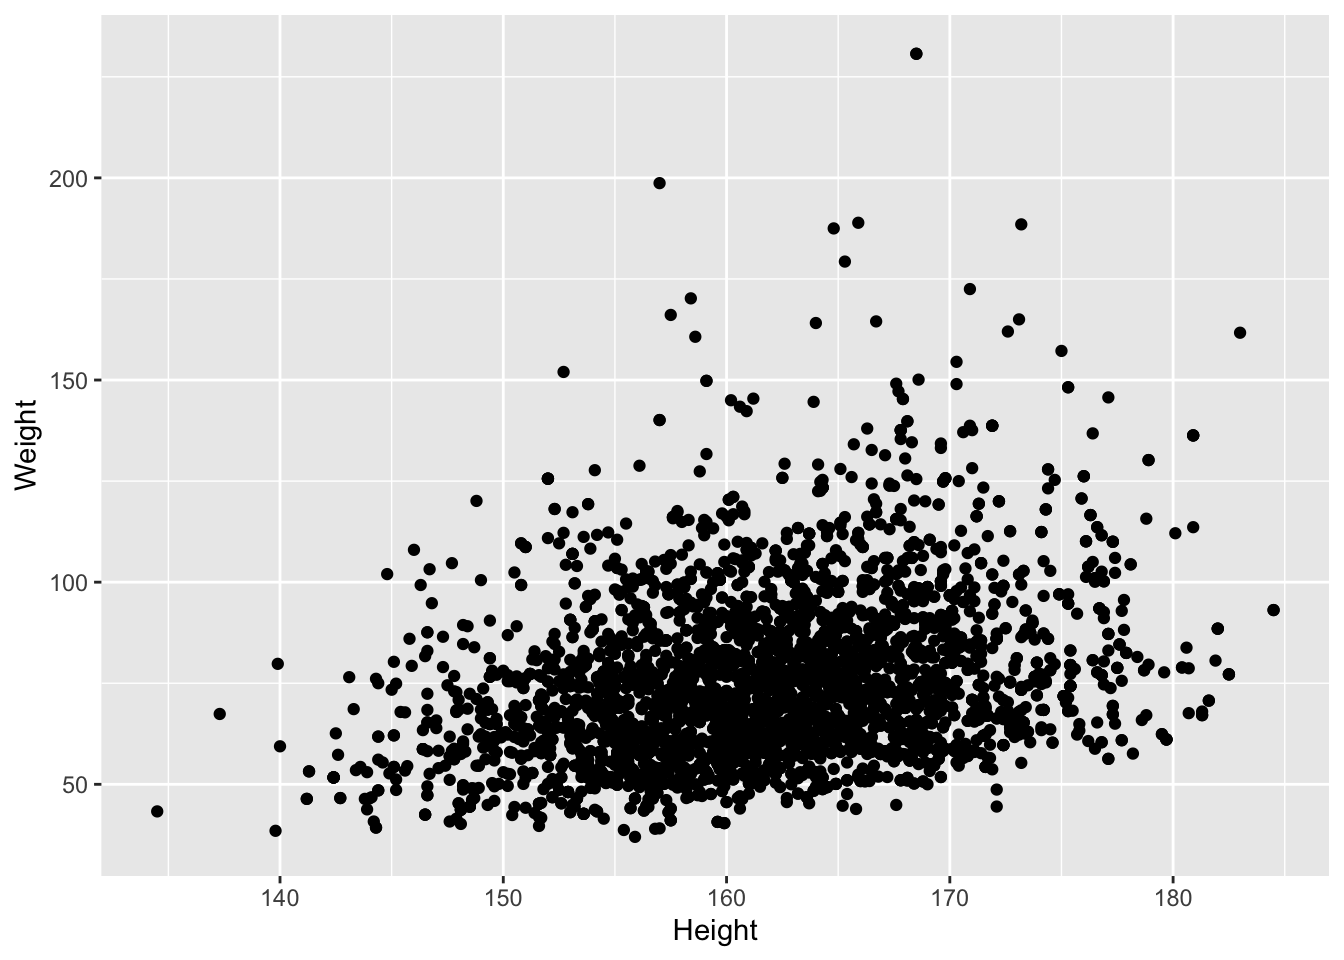
\includegraphics{Statistiek_2020_2021_files/figure-latex/unnamed-chunk-115-1.pdf}

Er is een duidelijke associatie tussen gewicht en lengte: als de lengte stijgt dan stijgt het gewicht gemiddeld ook. Er is echter veel variabiliteit en ook een indicatie dat het gewicht is scheef verdeeld naar rechts.

We exploreren eerst de data univariaat: variabele per variabele. Om een histogram en QQ-plot naast elkaar af te beelden slaan we de plots eerst op als een object en maken we gebruik van de \texttt{grid.arrange} functie van het gridExtra package om de plots naast elkaar te plotten.

\begin{Shaded}
\begin{Highlighting}[]
\NormalTok{p1 \textless{}{-}}\StringTok{ }\NormalTok{NHANES }\OperatorTok{\%\textgreater{}\%}\StringTok{ }\KeywordTok{filter}\NormalTok{(Age }\OperatorTok{\textgreater{}=}\StringTok{ }\DecValTok{18} \OperatorTok{\&}\StringTok{ }\NormalTok{Gender }\OperatorTok{==}\StringTok{ "female"}\NormalTok{) }\OperatorTok{\%\textgreater{}\%}\StringTok{ }
\StringTok{    }\KeywordTok{ggplot}\NormalTok{(}\KeywordTok{aes}\NormalTok{(}\DataTypeTok{x =}\NormalTok{ Height)) }\OperatorTok{+}\StringTok{ }\KeywordTok{geom\_histogram}\NormalTok{(}\KeywordTok{aes}\NormalTok{(}\DataTypeTok{y =}\NormalTok{ ..density.., }
    \DataTypeTok{fill =}\NormalTok{ ..count..)) }\OperatorTok{+}\StringTok{ }\KeywordTok{xlab}\NormalTok{(}\StringTok{"Height"}\NormalTok{) }\OperatorTok{+}\StringTok{ }\KeywordTok{ggtitle}\NormalTok{(}\StringTok{"All females in study"}\NormalTok{) }\OperatorTok{+}\StringTok{ }
\StringTok{    }\KeywordTok{geom\_density}\NormalTok{(}\KeywordTok{aes}\NormalTok{(}\DataTypeTok{y =}\NormalTok{ ..density..))}

\NormalTok{p2 \textless{}{-}}\StringTok{ }\NormalTok{NHANES }\OperatorTok{\%\textgreater{}\%}\StringTok{ }\KeywordTok{filter}\NormalTok{(Age }\OperatorTok{\textgreater{}=}\StringTok{ }\DecValTok{18} \OperatorTok{\&}\StringTok{ }\NormalTok{Gender }\OperatorTok{==}\StringTok{ "female"}\NormalTok{) }\OperatorTok{\%\textgreater{}\%}\StringTok{ }
\StringTok{    }\KeywordTok{ggplot}\NormalTok{(}\KeywordTok{aes}\NormalTok{(}\DataTypeTok{sample =}\NormalTok{ Height)) }\OperatorTok{+}\StringTok{ }\KeywordTok{geom\_qq}\NormalTok{() }\OperatorTok{+}\StringTok{ }\KeywordTok{geom\_qq\_line}\NormalTok{()}
\KeywordTok{grid.arrange}\NormalTok{(p1, p2, }\DataTypeTok{ncol =} \DecValTok{2}\NormalTok{)}
\end{Highlighting}
\end{Shaded}

\includegraphics{Statistiek_2020_2021_files/figure-latex/unnamed-chunk-116-1.pdf}

De lengte data zijn duidelijk approximatief normaal verdeeld.

\begin{Shaded}
\begin{Highlighting}[]
\NormalTok{p3 \textless{}{-}}\StringTok{ }\NormalTok{NHANES }\OperatorTok{\%\textgreater{}\%}\StringTok{ }\KeywordTok{filter}\NormalTok{(Age }\OperatorTok{\textgreater{}=}\StringTok{ }\DecValTok{18} \OperatorTok{\&}\StringTok{ }\NormalTok{Gender }\OperatorTok{==}\StringTok{ "female"}\NormalTok{) }\OperatorTok{\%\textgreater{}\%}\StringTok{ }
\StringTok{    }\KeywordTok{ggplot}\NormalTok{(}\KeywordTok{aes}\NormalTok{(}\DataTypeTok{x =}\NormalTok{ Weight)) }\OperatorTok{+}\StringTok{ }\KeywordTok{geom\_histogram}\NormalTok{(}\KeywordTok{aes}\NormalTok{(}\DataTypeTok{y =}\NormalTok{ ..density.., }
    \DataTypeTok{fill =}\NormalTok{ ..count..)) }\OperatorTok{+}\StringTok{ }\KeywordTok{xlab}\NormalTok{(}\StringTok{"Weight"}\NormalTok{) }\OperatorTok{+}\StringTok{ }\KeywordTok{ggtitle}\NormalTok{(}\StringTok{"All females in study"}\NormalTok{) }\OperatorTok{+}\StringTok{ }
\StringTok{    }\KeywordTok{geom\_density}\NormalTok{(}\KeywordTok{aes}\NormalTok{(}\DataTypeTok{y =}\NormalTok{ ..density..))}

\NormalTok{p4 \textless{}{-}}\StringTok{ }\NormalTok{NHANES }\OperatorTok{\%\textgreater{}\%}\StringTok{ }\KeywordTok{filter}\NormalTok{(Age }\OperatorTok{\textgreater{}=}\StringTok{ }\DecValTok{18} \OperatorTok{\&}\StringTok{ }\NormalTok{Gender }\OperatorTok{==}\StringTok{ "female"}\NormalTok{) }\OperatorTok{\%\textgreater{}\%}\StringTok{ }
\StringTok{    }\KeywordTok{ggplot}\NormalTok{(}\KeywordTok{aes}\NormalTok{(}\DataTypeTok{sample =}\NormalTok{ Weight)) }\OperatorTok{+}\StringTok{ }\KeywordTok{geom\_qq}\NormalTok{() }\OperatorTok{+}\StringTok{ }\KeywordTok{geom\_qq\_line}\NormalTok{()}

\KeywordTok{grid.arrange}\NormalTok{(p3, p4, }\DataTypeTok{ncol =} \DecValTok{2}\NormalTok{)}
\end{Highlighting}
\end{Shaded}

\includegraphics{Statistiek_2020_2021_files/figure-latex/unnamed-chunk-117-1.pdf}

De gewichtsdata zijn inderdaad scheef verdeeld!

Na log transformatie zijn de gewichtsdata minder scheef, maar nog steeds niet Normaal verdeeld.

\begin{Shaded}
\begin{Highlighting}[]
\NormalTok{p5 \textless{}{-}}\StringTok{ }\NormalTok{NHANES }\OperatorTok{\%\textgreater{}\%}\StringTok{ }\KeywordTok{filter}\NormalTok{(Age }\OperatorTok{\textgreater{}=}\StringTok{ }\DecValTok{18} \OperatorTok{\&}\StringTok{ }\NormalTok{Gender }\OperatorTok{==}\StringTok{ "female"}\NormalTok{) }\OperatorTok{\%\textgreater{}\%}\StringTok{ }
\StringTok{    }\KeywordTok{ggplot}\NormalTok{(}\KeywordTok{aes}\NormalTok{(}\DataTypeTok{x =}\NormalTok{ Weight }\OperatorTok{\%\textgreater{}\%}\StringTok{ }\NormalTok{log2)) }\OperatorTok{+}\StringTok{ }\KeywordTok{geom\_histogram}\NormalTok{(}\KeywordTok{aes}\NormalTok{(}\DataTypeTok{y =}\NormalTok{ ..density.., }
    \DataTypeTok{fill =}\NormalTok{ ..count..)) }\OperatorTok{+}\StringTok{ }\KeywordTok{xlab}\NormalTok{(}\StringTok{"Weight (log2)"}\NormalTok{) }\OperatorTok{+}\StringTok{ }\KeywordTok{ggtitle}\NormalTok{(}\StringTok{"All females in study"}\NormalTok{) }\OperatorTok{+}\StringTok{ }
\StringTok{    }\KeywordTok{geom\_density}\NormalTok{(}\KeywordTok{aes}\NormalTok{(}\DataTypeTok{y =}\NormalTok{ ..density..))}

\NormalTok{p6 \textless{}{-}}\StringTok{ }\NormalTok{NHANES }\OperatorTok{\%\textgreater{}\%}\StringTok{ }\KeywordTok{filter}\NormalTok{(Age }\OperatorTok{\textgreater{}=}\StringTok{ }\DecValTok{18} \OperatorTok{\&}\StringTok{ }\NormalTok{Gender }\OperatorTok{==}\StringTok{ "female"}\NormalTok{) }\OperatorTok{\%\textgreater{}\%}\StringTok{ }
\StringTok{    }\KeywordTok{ggplot}\NormalTok{(}\KeywordTok{aes}\NormalTok{(}\DataTypeTok{sample =}\NormalTok{ Weight }\OperatorTok{\%\textgreater{}\%}\StringTok{ }\NormalTok{log2)) }\OperatorTok{+}\StringTok{ }\KeywordTok{geom\_qq}\NormalTok{() }\OperatorTok{+}\StringTok{ }
\StringTok{    }\KeywordTok{geom\_qq\_line}\NormalTok{()}

\KeywordTok{grid.arrange}\NormalTok{(p5, p6, }\DataTypeTok{ncol =} \DecValTok{2}\NormalTok{)}
\end{Highlighting}
\end{Shaded}

\includegraphics{Statistiek_2020_2021_files/figure-latex/unnamed-chunk-118-1.pdf}

De scheefheid is er nog maar is sterk gereduceerd. We maken nu een plot van lengte in functie van het log\(_2\) getransformeerde gewicht.

\begin{Shaded}
\begin{Highlighting}[]
\NormalTok{NHANES }\OperatorTok{\%\textgreater{}\%}\StringTok{ }\KeywordTok{filter}\NormalTok{(Age }\OperatorTok{\textgreater{}=}\StringTok{ }\DecValTok{18} \OperatorTok{\&}\StringTok{ }\NormalTok{Gender }\OperatorTok{==}\StringTok{ "female"}\NormalTok{) }\OperatorTok{\%\textgreater{}\%}\StringTok{ }
\StringTok{    }\KeywordTok{ggplot}\NormalTok{(}\KeywordTok{aes}\NormalTok{(}\DataTypeTok{x =}\NormalTok{ Height, }\DataTypeTok{y =}\NormalTok{ Weight }\OperatorTok{\%\textgreater{}\%}\StringTok{ }\NormalTok{log2)) }\OperatorTok{+}\StringTok{ }
\StringTok{    }\KeywordTok{ylab}\NormalTok{(}\StringTok{"Weight (log2)"}\NormalTok{) }\OperatorTok{+}\StringTok{ }\KeywordTok{geom\_point}\NormalTok{()}
\end{Highlighting}
\end{Shaded}

\includegraphics{Statistiek_2020_2021_files/figure-latex/unnamed-chunk-119-1.pdf}

We introduceren nu een statistiek om de associatie te schatten: de correlatie.

\hypertarget{covariantie-en-correlatie}{%
\subsection{Covariantie en Correlatie}\label{covariantie-en-correlatie}}

Stel dat X en Y continue toevallig veranderlijken zijn

\begin{itemize}
\tightlist
\item
  Voor elk subject i observeren we dus \((X_i,Y_i)\).
\item
  Covariantie: hoe variëren \(X_i\) en \(Y_i\) rond hun gemiddelde \((E[X],E[Y])\)?
\end{itemize}

\[\mbox{Covar}(X,Y)=E[(X-E[X])(Y-E[Y])]\]

\begin{itemize}
\tightlist
\item
  De covariantie is dus de verwachte waarde van het product van de afwijking van de X waarde t.o.v. zijn verwachte waarde E{[}X{]} en de afwijking van de Y waarde t.o.v.zijn verwachte waarde E{[}Y{]}.
\end{itemize}

We kunnen de covariantie nu ook standardiseren zodat we een maat krijgen die voor elke dataset vergelijkbaar wordt: de correlatie. We doen dit door de covariantie te delen door de standaardafwijking van elke variabele:

\[\mbox{Cor}(X,Y)=\frac{E[(X-E[X])(Y-E[Y])]}{\sqrt{E[(X-E[X])^2}\sqrt{E[(Y-E[Y])^2}}\]

\hypertarget{pearson-correlatie}{%
\subsection{Pearson Correlatie}\label{pearson-correlatie}}

We introduceren nu een schatter voor de correlatie tussen twee continue toevallig veranderlijken op basis van de data in de steekproef:

\[
\mbox{Cor}(X,Y)=\frac{\sum_{i=1}^{n}(x_{i}-\bar{x})(y_{i}-\bar{y})}{(n-1)s_{x}s_{y}}
\]

We vervangen de verwachte waarden weer door het steekproefgemiddelden \(\bar x\) en \(\bar y\), en, we berekenen het gemiddeld product van de afwijkingen in x en y in de steekproef. Let op dat we hierbij weer corrigeren voor het aantal vrijheidsgraden. We geven elke observatie geen gewicht van 1/n maar van 1/(n-1). We hebben inderdaad het gemiddelde geschat, hier is dat gemiddelde bivariaat (het heeft een x en y coordinaat).

Deze schatter wordt ook wel de Pearson correlatie genoemd en heeft volgende eigenschappen:

\begin{itemize}
\item
  Er is een positieve correlatie wanneer \(y\) gemiddeld toeneemt bij een toename van: \(x \ \nearrow \ \Rightarrow \ y \ \nearrow\)
\item
  Er is een negatieve correlatie als \(y\) gemiddeld afneemt bij een toename in \(x\): \(x \ \nearrow \ \Rightarrow \ y \ \searrow\)
\item
  De correlatie ligt ook altijd tussen -1 en 1
\end{itemize}

In de figuur \ref{fig:bijdrageCor} wordt de bijdrage weergegeven van individuele metingen in de correlatie. Als punten in het 1ste en 3de kwadrant liggen is er een negatieve bijdrage van de observatie in de correlatie, als ze in het 2de en 4de kwadrant liggen is er een positieve bijdrage.

\begin{figure}
\centering
\includegraphics{Statistiek_2020_2021_files/figure-latex/bijdrageCor-1.pdf}
\caption{\label{fig:bijdrageCor}Bijdrage van individuele metingen in de correlatie.}
\end{figure}

We berekenen vervolgens de correlatie voor lengte, gewicht en het log getransformeerde gewicht.

\begin{Shaded}
\begin{Highlighting}[]
\NormalTok{NHANES }\OperatorTok{\%\textgreater{}\%}\StringTok{ }\KeywordTok{filter}\NormalTok{(Age }\OperatorTok{\textgreater{}=}\StringTok{ }\DecValTok{18} \OperatorTok{\&}\StringTok{ }\NormalTok{Gender }\OperatorTok{==}\StringTok{ "female"}\NormalTok{) }\OperatorTok{\%\textgreater{}\%}\StringTok{ }
\StringTok{    }\KeywordTok{select}\NormalTok{(Weight, Height) }\OperatorTok{\%\textgreater{}\%}\StringTok{ }\KeywordTok{mutate}\NormalTok{(}\DataTypeTok{log2Weight =}\NormalTok{ Weight }\OperatorTok{\%\textgreater{}\%}\StringTok{ }
\StringTok{    }\NormalTok{log2) }\OperatorTok{\%\textgreater{}\%}\StringTok{ }\NormalTok{na.exclude }\OperatorTok{\%\textgreater{}\%}\StringTok{ }\NormalTok{cor}
\end{Highlighting}
\end{Shaded}

\begin{verbatim}
##               Weight    Height log2Weight
## Weight     1.0000000 0.2845792  0.9811638
## Height     0.2845792 1.0000000  0.3074578
## log2Weight 0.9811638 0.3074578  1.0000000
\end{verbatim}

Merk op dat:

\begin{itemize}
\tightlist
\item
  De correlatie lager is als de data niet worden getransformeerd.
\item
  De Pearson correlatie is gevoelig voor outliers!
\item
  Gebruik de Pearson correlatie niet voor scheef verdeelde data of data met outliers!
\end{itemize}

\hypertarget{impact-van-outliers}{%
\subsubsection{Impact van outliers}\label{impact-van-outliers}}

In figuur \ref{fig:corOutlier} wordt de impact van outliers op de Pearson correlatie geïllustreerd d.m.v. gesimuleerde data met één outlier. We zien dat de correlatie bijna halveert ten gevolge van de outlier!

\begin{Shaded}
\begin{Highlighting}[]
\KeywordTok{set.seed}\NormalTok{(}\DecValTok{100}\NormalTok{)}
\NormalTok{x \textless{}{-}}\StringTok{ }\KeywordTok{rnorm}\NormalTok{(}\DecValTok{20}\NormalTok{)}
\NormalTok{simData \textless{}{-}}\StringTok{ }\KeywordTok{data.frame}\NormalTok{(}\DataTypeTok{x =}\NormalTok{ x, }\DataTypeTok{y =}\NormalTok{ x }\OperatorTok{*}\StringTok{ }\DecValTok{2} \OperatorTok{+}\StringTok{ }\KeywordTok{rnorm}\NormalTok{(}\KeywordTok{length}\NormalTok{(x)))}
\NormalTok{p1 \textless{}{-}}\StringTok{ }\NormalTok{simData }\OperatorTok{\%\textgreater{}\%}\StringTok{ }\KeywordTok{ggplot}\NormalTok{(}\KeywordTok{aes}\NormalTok{(}\DataTypeTok{x =}\NormalTok{ x, }\DataTypeTok{y =}\NormalTok{ y)) }\OperatorTok{+}\StringTok{ }\KeywordTok{geom\_point}\NormalTok{() }\OperatorTok{+}\StringTok{ }
\StringTok{    }\KeywordTok{ggtitle}\NormalTok{(}\KeywordTok{paste}\NormalTok{(}\StringTok{"cor ="}\NormalTok{, }\KeywordTok{cor}\NormalTok{(simData[, }\DecValTok{1}\NormalTok{], simData[, }
        \DecValTok{2}\NormalTok{]) }\OperatorTok{\%\textgreater{}\%}\StringTok{ }\KeywordTok{round}\NormalTok{(., }\DecValTok{2}\NormalTok{)))}

\NormalTok{outlier \textless{}{-}}\StringTok{ }\KeywordTok{rbind}\NormalTok{(simData, }\KeywordTok{c}\NormalTok{(}\DecValTok{2}\NormalTok{, }\DecValTok{{-}4}\NormalTok{))}
\NormalTok{p2 \textless{}{-}}\StringTok{ }\NormalTok{outlier }\OperatorTok{\%\textgreater{}\%}\StringTok{ }\KeywordTok{ggplot}\NormalTok{(}\KeywordTok{aes}\NormalTok{(}\DataTypeTok{x =}\NormalTok{ x, }\DataTypeTok{y =}\NormalTok{ y)) }\OperatorTok{+}\StringTok{ }\KeywordTok{geom\_point}\NormalTok{() }\OperatorTok{+}\StringTok{ }
\StringTok{    }\KeywordTok{ggtitle}\NormalTok{(}\KeywordTok{paste}\NormalTok{(}\StringTok{"cor ="}\NormalTok{, }\KeywordTok{cor}\NormalTok{(outlier[, }\DecValTok{1}\NormalTok{], outlier[, }
        \DecValTok{2}\NormalTok{]) }\OperatorTok{\%\textgreater{}\%}\StringTok{ }\KeywordTok{round}\NormalTok{(., }\DecValTok{2}\NormalTok{)))}

\KeywordTok{grid.arrange}\NormalTok{(p1, p2, }\DataTypeTok{ncol =} \DecValTok{2}\NormalTok{)}
\end{Highlighting}
\end{Shaded}

\begin{figure}
\centering
\includegraphics{Statistiek_2020_2021_files/figure-latex/corOutlier-1.pdf}
\caption{\label{fig:corOutlier}Correlatie van gesimuleerde data met 1 outlier}
\end{figure}

\hypertarget{de-pearson-correlatie-pikt-enkel-linear-associatie-op}{%
\subsubsection{De Pearson correlatie pikt enkel linear associatie op}\label{de-pearson-correlatie-pikt-enkel-linear-associatie-op}}

In figuur \ref{fig:corQuad} simuleren we data met een kwadratisch verband en observeren we dat de correlatie bijna nul is!

\begin{Shaded}
\begin{Highlighting}[]
\NormalTok{x \textless{}{-}}\StringTok{ }\KeywordTok{rnorm}\NormalTok{(}\DecValTok{100}\NormalTok{)}
\NormalTok{quadratic \textless{}{-}}\StringTok{ }\KeywordTok{data.frame}\NormalTok{(}\DataTypeTok{x =}\NormalTok{ x, }\DataTypeTok{y =}\NormalTok{ x}\OperatorTok{\^{}}\DecValTok{2} \OperatorTok{+}\StringTok{ }\KeywordTok{rnorm}\NormalTok{(}\KeywordTok{length}\NormalTok{(x)))}
\NormalTok{quadratic }\OperatorTok{\%\textgreater{}\%}\StringTok{ }\KeywordTok{ggplot}\NormalTok{(}\KeywordTok{aes}\NormalTok{(}\DataTypeTok{x =}\NormalTok{ x, }\DataTypeTok{y =}\NormalTok{ y)) }\OperatorTok{+}\StringTok{ }\KeywordTok{geom\_point}\NormalTok{() }\OperatorTok{+}\StringTok{ }
\StringTok{    }\KeywordTok{ggtitle}\NormalTok{(}\KeywordTok{paste}\NormalTok{(}\StringTok{"cor ="}\NormalTok{, }\KeywordTok{cor}\NormalTok{(quadratic[, }\DecValTok{1}\NormalTok{], quadratic[, }
        \DecValTok{2}\NormalTok{]) }\OperatorTok{\%\textgreater{}\%}\StringTok{ }\KeywordTok{round}\NormalTok{(., }\DecValTok{2}\NormalTok{))) }\OperatorTok{+}\StringTok{ }\KeywordTok{geom\_hline}\NormalTok{(}\DataTypeTok{yintercept =} \KeywordTok{mean}\NormalTok{(quadratic[, }
    \DecValTok{2}\NormalTok{]), }\DataTypeTok{col =} \StringTok{"red"}\NormalTok{) }\OperatorTok{+}\StringTok{ }\KeywordTok{geom\_vline}\NormalTok{(}\DataTypeTok{xintercept =} \KeywordTok{mean}\NormalTok{(quadratic[, }
    \DecValTok{1}\NormalTok{]), }\DataTypeTok{col =} \StringTok{"red"}\NormalTok{)}
\end{Highlighting}
\end{Shaded}

\begin{figure}
\centering
\includegraphics{Statistiek_2020_2021_files/figure-latex/corQuad-1.pdf}
\caption{\label{fig:corQuad}Correlatie van gesimuleerde data met een kwadratisch verband. De data in de bovenste kwadranten compenseren elkaar als het ware alsook in de onderste kwadranten (ongeveer evenveel positieve en negatieve bijdragen door de data in de correlatie)}
\end{figure}

\hypertarget{verschillende-groottes-van-correlatie}{%
\subsection{Verschillende groottes van correlatie}\label{verschillende-groottes-van-correlatie}}

Om een inzicht te krijgen in de grootte van de correlatie, simuleren we data met een verschillende correlatie. We geven telkens de correlatie weer boven de plot. Hoe sterker de correlatie hoe meer de puntenwolk naar een lineair verband toegaat.

\includegraphics{Statistiek_2020_2021_files/figure-latex/unnamed-chunk-121-1.pdf} \includegraphics{Statistiek_2020_2021_files/figure-latex/unnamed-chunk-121-2.pdf}

\hypertarget{spearman-correlatie}{%
\subsection{Spearman correlatie}\label{spearman-correlatie}}

De Spearman correlatie is de Pearson correlatie na transformatie van de data naar ranks. Hierdoor wordt deze schatter minder gevoelig voor outliers.

\begin{itemize}
\tightlist
\item
  Pearson correlatie
\end{itemize}

\begin{Shaded}
\begin{Highlighting}[]
\KeywordTok{cor}\NormalTok{(outlier)}
\end{Highlighting}
\end{Shaded}

\begin{verbatim}
##           x         y
## x 1.0000000 0.4682823
## y 0.4682823 1.0000000
\end{verbatim}

\begin{itemize}
\tightlist
\item
  Spearman correlatie
\end{itemize}

\begin{Shaded}
\begin{Highlighting}[]
\KeywordTok{cor}\NormalTok{(outlier, }\DataTypeTok{method =} \StringTok{"spearman"}\NormalTok{)}
\end{Highlighting}
\end{Shaded}

\begin{verbatim}
##           x         y
## x 1.0000000 0.6571429
## y 0.6571429 1.0000000
\end{verbatim}

We verifiëren dat de Spearman correlatie de Pearson correlatie is van rang getransformeerde data. Die wordt bekomen door de observaties te ordenen van klein naar groot en elke observatie te vervangen door zijn rangorde.

\begin{Shaded}
\begin{Highlighting}[]
\NormalTok{rankData \textless{}{-}}\StringTok{ }\KeywordTok{apply}\NormalTok{(outlier, }\DecValTok{2}\NormalTok{, rank)}
\KeywordTok{cor}\NormalTok{(rankData)}
\end{Highlighting}
\end{Shaded}

\begin{verbatim}
##           x         y
## x 1.0000000 0.6571429
## y 0.6571429 1.0000000
\end{verbatim}

We berekenen nu de Spearman correlatie in de NHANES studie.
We observeren dat de correlatie tussen lengte en gewicht, en lengte en log2 getransformeerd gewicht exact gelijk is.
Dat is logisch want de log-transformatie is een monotone transformatie en verandert de ordening van de data dus niet, de ranks van gewicht en deze van het log gewicht zijn identiek!

\begin{Shaded}
\begin{Highlighting}[]
\NormalTok{NHANES }\OperatorTok{\%\textgreater{}\%}\StringTok{ }\KeywordTok{filter}\NormalTok{(Age }\OperatorTok{\textgreater{}=}\StringTok{ }\DecValTok{18} \OperatorTok{\&}\StringTok{ }\NormalTok{Gender }\OperatorTok{==}\StringTok{ "female"}\NormalTok{) }\OperatorTok{\%\textgreater{}\%}\StringTok{ }
\StringTok{    }\KeywordTok{select}\NormalTok{(Weight, Height) }\OperatorTok{\%\textgreater{}\%}\StringTok{ }\KeywordTok{mutate}\NormalTok{(}\DataTypeTok{log2Weight =}\NormalTok{ Weight }\OperatorTok{\%\textgreater{}\%}\StringTok{ }
\StringTok{    }\NormalTok{log2) }\OperatorTok{\%\textgreater{}\%}\StringTok{ }\NormalTok{na.exclude }\OperatorTok{\%\textgreater{}\%}\StringTok{ }\KeywordTok{cor}\NormalTok{(}\DataTypeTok{method =} \StringTok{"spearman"}\NormalTok{)}
\end{Highlighting}
\end{Shaded}

\begin{verbatim}
##               Weight    Height log2Weight
## Weight     1.0000000 0.2892776  1.0000000
## Height     0.2892776 1.0000000  0.2892776
## log2Weight 1.0000000 0.2892776  1.0000000
\end{verbatim}

Bij het interpreteren van correlaties, alsook bij het uitvoeren van
regressie-analyses in de volgende secties, zijn de volgende waarschuwingen
van zeer groot belang:

\begin{enumerate}
\def\labelenumi{\arabic{enumi}.}
\item
  Correlaties zijn het makkelijkst te interpreteren tussen 2 groepen Normaal verdeelde observaties. Een kleine training laat immers toe om snel inzicht te krijgen in de grootte van de correlatiecoëfficiënt zonder zich verder over de specifieke verdeling te hoeven bekommeren. In het bijzonder kan men voor Normaal verdeelde observaties visueel inzicht krijgen in de sterkte van de correlatie door een ellips rond de puntenwolk te tekenen die (nagenoeg) alle punten bevat. Als de ellips op een cirkel lijkt, dan is er geen correlatie. Hoe dunner de ellips, hoe sterker de correlatie. De oriëntatie van de ellips geeft hierbij het teken van de correlatie weer.
\item
  Voor niet-Normale gegevens hangt de betekenis van een correlatiecoëfficiënt van zekere grootte, nauw samen met de specifieke vorm van de verdeling. Wanneer de 2 variabelen die we onderzoeken niet Normaal verdeeld zijn, dan zijn er 2 mogelijkheden om een zinvolle correlatiecoëfficiënt weer te geven. Variabelen die scheef verdeeld zijn, kan men transformeren (bvb. een log-transformatie) in de hoop dat de getransformeerde gegevens bij benadering Normaal verdeeld zijn en lineair samenhangen.
\item
  Merk op dat een correlatiecoëfficiënt van 0 tussen 2 variabelen \(X\) en \(Y\) niet noodzakelijk impliceert dat deze variabelen onafhankelijk zijn. Zie kwadratisch verband! Daarom is het van belang om de aard van samenhang tussen 2 variabelen steeds te onderzoeken via een scatterplot alvorens een correlatiecoëfficiënt te rapporteren. Wanneer het verband monotoon is, maar sterk niet-lineair is, dan is het aangewezen om niet de Pearson correlatiecoëfficiënt, maar Spearman's correlatiecoëfficiënt te rapporteren. Indien het verband niet-monotoon is, dan zijn correlatiecoëfficiënten niet geschikt en moet men overstappen op meer geavanceerde regressietechnieken.
\item
  Bij jonge kinderen is de grootte van hun schoenmaat uiteraard sterk gecorreleerd met hun leescapaciteiten. Dat op zich impliceert echter niet dat het leren van nieuwe woorden hun voeten doet groeien of dat het groeien van hun voeten impliceert dat ze beter kunnen lezen. Ook algemeen\footnote{In het Engels is dit welbekend onder de zinsnede \emph{`Association is not causation!'}.} hoeft een correlatie tussen 2 variabelen niet te impliceren dat er een causaal verband is. De relatie tussen 2 metingen kan immers sterk verstoord worden door confounders (bvb. de leeftijd in bovenstaand voorbeeld). Hoewel dit overduidelijk is in bovenstaand voorbeeld, is het in vele andere contexten veel minder duidelijk en worden er, vooral in de populaire literatuur, vaak causale beweringen gemaakt die niet (volledig) door de gegevens worden gestaafd. Volgend voorbeeld illustreert dit. Denk hierbij aan het voorbeeld van de associatie van groente consumptie en covid mortaliteit.
\item
  Een \emph{ecologische analyse} is een statistische analyse waarbij men associaties bestudeert tussen samenvattingsmaten (zoals gemiddelden, incidenties, \ldots) die reeds berekend werden voor groepen subjecten. Dit is het geval bij het covid voorbeeld uit de introductie waarbij men mortaliteit modellereert in functie van de gemiddelde dagelijkse groenteconsumptie per capita in verschillende landen. Wanneer men aldus een \emph{ecologische correlatie} vaststelt voor groepen subjecten of individuen (in dit geval,landen), impliceert dat niet noodzakelijk dat deze correlatie ook voor de subjecten zelf opgaat\footnote{In het Engels is dit welbekend onder de naam \emph{`ecological fallacy'}.}. Volgend voorbeeld illustreert dit.
\end{enumerate}

\begin{example}[Ecological fallacy]
\protect\hypertarget{exm:unnamed-chunk-126}{}{\label{exm:unnamed-chunk-126} \iffalse (Ecological fallacy) \fi{} }
\end{example}

Voor de 48 staten in de V.S. werden telkens 2 getallen
berekend: het percentage van de mensen die in een ander land geboren zijn en het percentage geletterden. De correlatie ertussen bedraagt 0.53 (Robinson, 1950). Dit is een \emph{ecologische correlatie} omdat de eenheid van de analyse de groep residenten uit een zelfde staat is, en niet de individuele residenten zelf. Deze ecologische correlatie suggereert dat mensen van vreemde afkomst doorgaans beter geschoold zijn (in Amerikaans Engels) dan de oorspronkelijke inwoners. Wanneer men echter de correlatie berekent op basis
van de gegevens voor alle individuele residenten, bekomt men -0.11. De ecologische analyse is hier duidelijk misleidend: het teken van de correlatie is er positief omdat mensen van vreemde origine de neiging hebben om te gaan wonen in staten waar de oorspronkelijke bevolking relatief goed geschoold is.

\textbf{Einde voorbeeld}

\hypertarget{sec:missing}{%
\section{Onvolledige gegevens}\label{sec:missing}}

Het gebeurt vaak in de biowetenschappen dat, ondanks zorgvuldig veld- en laboratoriumwerk, metingen die men plande te verzamelen, niet bekomen werden. Men noemt deze dan \emph{ontbrekende gegevens} of \emph{missing data (points)}.

Minder drastisch, kunnen observaties soms slechts ten dele gekend zijn.
Bijvoorbeeld bij een studie van de overlevingsduur van dieren en planten wacht men niet steeds tot
alle subjecten gestorven zijn. Op het eind van de studie zal men bijvoorbeeld voor een 50-jarige
olifant die in leven is, slechts weten dat de overlevingstijd
minstens 50 jaar bedraagt, maar niet de exacte waarde kennen. Zo'n gegeven
wordt \emph{rechts-gecensureerd} genoemd: we weten dat de gewenste
observatie rechts van 50 ligt, maar verder niets meer.

Analoog kunnen observaties \emph{links-gecensureerd} zijn. Bij het meten
van bepaalde concentraties kan een detectielimiet bestaan: een ondergrens beneden
dewelke het meettoestel geen aanwezigheid kan detecteren. Men weet in zo'n
geval dat de concentratie kleiner dan die ondergrens is, maar niet hoeveel
kleiner.

Tenslotte vermelden we nog \emph{interval-gecensureerde} gegevens. Bij het
screenen naar HIV bijvoorbeeld, zal men weten dat een subject seropositief
geworden is ergens tussen de laatste negatieve HIV test en de eerste
positieve HIV test, maar het exacte tijdstip van seroconversie blijft
onbekend.

De aanwezigheid van gegevens die niet of slechts partieel zijn opgemeten zorgt
altijd voor extra moeilijkheden bij de analyse en interpretatie van de
onderzoeksresultaten. Dat is omdat de missende gegevens mogelijks afkomstig zijn
van een speciale populatie. Dat is het meest duidelijk in klinische experimenten bij mensen.
Patiënten zullen hier vaak de studie verlaten wanneer
ze genezen zijn, in welk geval men de metingen van deze patiënten niet te
zien krijgt. Dit negeren door enkel de aanwezige gegevens te analyseren, zal
de resultaten er slechter doen uitzien dan ze in werkelijkheid zijn. Meestal
houdt dat immers de veronderstelling in dat de aanwezige gegevens representatief blijven
voor de populatie die men wenst te bestuderen. Dit kan in sommige gevallen
de resultaten sterk vertekenen. In de statistische literatuur zijn de
laatste jaren heel wat complexe technieken ontwikkeld om hiervoor te
corrigeren. Deze technieken worden meer en meer in de statistische software
ingebouwd en recent heeft ook R verschillende bibliotheken toegevoegd.
Het is
echter aangewezen om voor het gebruik van deze gevorderde technieken een
statisticus te consulteren.

\hypertarget{clips-over-de-code-in-dit-hoofdstuk}{%
\section{Clips over de code in dit hoofdstuk}\label{clips-over-de-code-in-dit-hoofdstuk}}

\begin{enumerate}
\def\labelenumi{\arabic{enumi}.}
\tightlist
\item
  Univariate exploratie van continue variabelen
\end{enumerate}

\begin{enumerate}
\def\labelenumi{\arabic{enumi}.}
\setcounter{enumi}{1}
\tightlist
\item
  Beschrijvende statistiek
\end{enumerate}

\begin{enumerate}
\def\labelenumi{\arabic{enumi}.}
\setcounter{enumi}{2}
\tightlist
\item
  Normale benadering
\end{enumerate}

\begin{enumerate}
\def\labelenumi{\arabic{enumi}.}
\setcounter{enumi}{3}
\tightlist
\item
  Associatie van twee continue Variabelen
\end{enumerate}

\hypertarget{chap:besluit}{%
\chapter{Statistische besluitvorming}\label{chap:besluit}}

Alle kennisclips die in dit hoofdstuk zijn verwerkt kan je in deze youtube playlist vinden:

\begin{itemize}
\item
  \href{https://www.youtube.com/playlist?list=PLZH1hP8_LbJKyD9Jw5cqd-btYs11f9tkz}{Kennisclips Hoofdstuk5 Puntschatters en Intervalschatters}
\item
  \href{https://www.youtube.com/playlist?list=PLZH1hP8_LbJKEtDy2errIWf8hLJODw-jK}{Kennisclips Hoofdstuk5 Hypothesetoetsen}
\end{itemize}

Link naar webpage/script die wordt gebruik in de kennisclips:

\begin{itemize}
\item
  \href{https://statomics.github.io/sbc20/rmd/05-statisticalInference.html}{script Hoofdstuk5}
\item
  \href{https://statomics.github.io/sbc20/rmd/05-statisticalInference-twosampleT.html}{script Hoofdstuk5: Two-sample t-test}
\end{itemize}

\hypertarget{inleiding-4}{%
\section{Inleiding}\label{inleiding-4}}

In dit hoofdstuk zullen we werken rond de \emph{Captopril dataset}.
Captopril is een medicijn dat wordt voorgeschreven bij hypertensie en chronisch hartfalen. Het behoort tot de klasse van ACE remmers die activiteit van het renine-angiotensine-aldosteronsysteem onderdrukken. Dat systeem zet het hormoon angiotensineI om in angiotensine II, die een krachtige vaatvernauwende werking heeft. ACE remmers verminderen de omzetting van angiotensine I naar angiotensine II waardoor de vaatvernauwing wordt onderdrukt. Tijdens de ontwikkeling van het medicijn werd een eerste kleine studie opgezet om na te gaan of captopril een bloeddrukverlagend effect heeft bij patiënten met hypertensie.

Observaties bij een klein aantal subjecten mogen een onderzoeker er dan al van overtuigen iets nieuws te hebben ontdekt, maar om anderen te overtuigen zijn objectieve, wetenschappelijke argumenten nodig.
Vooreerst moeten de
resultaten voldoende \emph{representatief} zijn, d.w.z. veralgemeenbaar
naar een ruime biologische populatie (bvb. naar de volledige populatie van patiënten met hypertensie).
Ten tweede moet er rekening mee gehouden worden dat de resultaten \emph{variabel} zijn, d.w.z. dat men
door toeval doorgaans andere resultaten zou vinden indien men een andere, vergelijkbare
groep subjecten zou analyseren.
Om die reden is het belangrijk om uit te drukken in welke mate de resultaten
(bvb. de geschatte bloeddrukdaling) zouden variëren van steekproef tot steekproef en of men op basis van de steekproef kan aantonen dat er een effect is van een behandeling (b.v. dat het middel captopril bloeddrukverlagend werkt in de populatie).
Dit vormt het doel van dit hoofdstuk.

Om een representatieve groep subjecten te waarborgen, vertrekt een goede
onderzoeksopzet vanuit een belangrijke, precies geformuleerde vraagstelling
omtrent een duidelijk omschreven populatie.

Zoals eerder in de cursus aangegeven, zal men in de praktijk om financiële en logistieke redenen bijna nooit een
volledige populatie kunnen bestuderen.
Populatieparameters kunnen daarom meestal
niet exact bepaald worden. Enkel een deel van de populatie kan onderzocht
worden, wat men een \emph{steekproef} noemt. Volgens een
gestructureerd design worden daartoe lukraak subjecten uit de doelpopulatie
getrokken en geobserveerd. De onbekende parameters worden vervolgens geschat
o.b.v. die steekproef en noemt men schattingen. In de praktijk hoopt men uiteraard dat de schattingen die men bekomt op basis van de steekproef vergelijkbaar zijn met de overeenkomstige populatieparameters die men voor de volledige populatie zou bekomen.\\
Typisch kan de onderzoeksvraag worden vertaald naar een populatieparameter.
Ze kan bijvoorbeeld worden uitgedrukt in termen van een populatiegemiddelde, bijvoorbeeld de gemiddelde bloeddrukverandering na de inname van captopril bij patiënten met hypertensie.

\hypertarget{captopril-voorbeeld}{%
\section{Captopril voorbeeld}\label{captopril-voorbeeld}}

Onderzoekers wensen na te gaan of het medicijn Captopril een bloeddruk verlagend effect heeft.
De onderzoekers wensen uitspraken te kunnen doen over het effect van captopril op de systolische bloeddruk van huidige en toekomstige patiënten met hypertensie, m.a.w. ze wensen uitspraken te doen over het effect van captopril op het niveau van de \emph{Populatie}.
Ze zullen hiervoor een experiment opzetten om het effect van captopril bestuderen (\emph{Proefopzet}) waarbij een \emph{steekproef} (sample) van de patiënten met hypertensie is getrokken uit de populatie.
Vervolgens zullen ze de data exploreren en het effect van captopril besturen in de steekproef (\emph{Data Exploratie \& Beschrijvende Statistiek}). Op basis van de steekproef zullen ze dan het effect van captopril \emph{Schatten} in de populatie en zullen ze a.d.h.v. methoden uit \emph{Statistische besluitvorming}\footnote{Ook wel Statistische Inferentie genoemd} nagaan in hoeverre de geobserveerde effecten in de steekproef veralgemeend kunnen worden naar de algemene populatie toe.

Deze verschillende stappen worden geïllustreerd in Figuur \ref{fig:captoPop2Samp2Pop}.

\begin{figure}

{\centering \includegraphics[width=1\linewidth]{Statistiek_2020_2021_files/figure-latex/captoPop2Samp2Pop-1} 

}

\caption{Verschillende stappen in de captopril studie.}\label{fig:captoPop2Samp2Pop}
\end{figure}

\hypertarget{proefopzet}{%
\subsection{Proefopzet}\label{proefopzet}}

Bij proefopzet zullen we een gestructureerd design voorstellen om lukraak subjecten uit de doelpopulatie
te selecteren, toe te wijzen aan een behandeling en te observeren.
We zullen hierbij een response variabele meten, een karakteristiek van interesse. In het captopril voorbeeld is dit de systolische bloeddruk.

In de captopril studie hebben de onderzoekers gebruik gemaakt van een een pre-test/post-test design.
De patiënten werden at random gekozen uit de populatie.
Van elke patiënt in de studie werd de systolische en diasystolische bloeddruk gemeten voor en na het toedienen van captopril.
Het pre-test/post-test design heeft als voordeel dat we het effect van het toedienen van captopril op de bloeddruk kunnen meten voor elke patiënt. Een nadeel daarentegen is dat er geen controle behandeling is waardoor we een mogelijkse bloeddrukverlaging niet noodzakelijkerwijs kunnen toeschrijven aan de werking van captopril. Er zou immers ook een placebo-effect kunnen optreden waardoor de bloeddruk van de patiënt daalt omdat men weet dat men een medicijn kreeg tegen een hoge bloeddruk.

\hypertarget{data-exploratie-beschrijvende-statistiek}{%
\subsection{Data Exploratie \& Beschrijvende Statistiek}\label{data-exploratie-beschrijvende-statistiek}}

Eens de data zijn geobserveerd, is het belangrijk om deze te exploreren om inzicht te krijgen in hun verdeling en karakteristieken.
Vervolgens zullen we de gegevens samenvatten zodat we het effect van interesse kunnen kwantificeren in de steekproef.
In deze studie is de systolische bloeddruk en de diasystolische bloeddruk gemeten voor elke patiënt voor en na het toedienen van captopril.
De data is beschikbaar in een tekstbestand met naam \texttt{captopril.txt} op de github pagina \url{https://raw.githubusercontent.com/statOmics/sbc20/master/data/captopril.txt}.
We zullen eerst exploreren welke figuren nuttig zijn in onze context.
In wetenschappelijke artikels worden vaak figuren gemaakt van het gemiddelde en de standaardafwijking (zie Figuur \ref{fig:captoBar}).

\begin{Shaded}
\begin{Highlighting}[]
\CommentTok{\# Eerst lezen we de data in. Deze bevindt zich in}
\CommentTok{\# de subdirectory dataset Het is een tekstbestand}
\CommentTok{\# waarbij de kolommen van elkaar gescheiden zijn}
\CommentTok{\# d.m.v kommas. sep=\textquotesingle{},\textquotesingle{} De eerste rij bevat de}
\CommentTok{\# namen van de variabelen}
\NormalTok{captopril \textless{}{-}}\StringTok{ }\KeywordTok{read.table}\NormalTok{(}\StringTok{"https://raw.githubusercontent.com/statOmics/sbc20/master/data/captopril.txt"}\NormalTok{, }
    \DataTypeTok{header =} \OtherTok{TRUE}\NormalTok{, }\DataTypeTok{sep =} \StringTok{","}\NormalTok{)}
\KeywordTok{head}\NormalTok{(captopril)}
\end{Highlighting}
\end{Shaded}

\begin{verbatim}
##   id SBPb DBPb SBPa DBPa
## 1  1  210  130  201  125
## 2  2  169  122  165  121
## 3  3  187  124  166  121
## 4  4  160  104  157  106
## 5  5  167  112  147  101
## 6  6  176  101  145   85
\end{verbatim}

\begin{Shaded}
\begin{Highlighting}[]
\NormalTok{captoprilTidy \textless{}{-}}\StringTok{ }\NormalTok{captopril }\OperatorTok{\%\textgreater{}\%}\StringTok{ }\KeywordTok{gather}\NormalTok{(type, bp, }\OperatorTok{{-}}\NormalTok{id)}
\NormalTok{captoprilTidy }\OperatorTok{\%\textgreater{}\%}\StringTok{ }\KeywordTok{group\_by}\NormalTok{(type) }\OperatorTok{\%\textgreater{}\%}\StringTok{ }\KeywordTok{summarize\_at}\NormalTok{(}\StringTok{"bp"}\NormalTok{, }
    \KeywordTok{list}\NormalTok{(}\DataTypeTok{mean =} \OperatorTok{\textasciitilde{}}\KeywordTok{mean}\NormalTok{(., }\DataTypeTok{na.rm =} \OtherTok{TRUE}\NormalTok{), }\DataTypeTok{sd =} \OperatorTok{\textasciitilde{}}\KeywordTok{sd}\NormalTok{(., }
        \DataTypeTok{na.rm =} \OtherTok{TRUE}\NormalTok{), }\DataTypeTok{n =} \ControlFlowTok{function}\NormalTok{(x) x }\OperatorTok{\%\textgreater{}\%}\StringTok{ }\NormalTok{is.na }\OperatorTok{\%\textgreater{}\%}\StringTok{ }
\StringTok{        \textasciigrave{}}\DataTypeTok{!}\StringTok{\textasciigrave{}} \OperatorTok{\%\textgreater{}\%}\StringTok{ }\NormalTok{sum)) }\OperatorTok{\%\textgreater{}\%}\StringTok{ }\KeywordTok{mutate}\NormalTok{(}\DataTypeTok{se =}\NormalTok{ sd}\OperatorTok{/}\KeywordTok{sqrt}\NormalTok{(n))}
\end{Highlighting}
\end{Shaded}

\begin{verbatim}
## # A tibble: 4 x 5
##   type   mean    sd     n    se
##   <chr> <dbl> <dbl> <int> <dbl>
## 1 DBPa   103.  12.6    15  3.24
## 2 DBPb   112.  10.5    15  2.70
## 3 SBPa   158   20.0    15  5.16
## 4 SBPb   177.  20.6    15  5.31
\end{verbatim}

\begin{Shaded}
\begin{Highlighting}[]
\NormalTok{captoprilTidy }\OperatorTok{\%\textgreater{}\%}\StringTok{ }\KeywordTok{group\_by}\NormalTok{(type) }\OperatorTok{\%\textgreater{}\%}\StringTok{ }\KeywordTok{summarize\_at}\NormalTok{(}\StringTok{"bp"}\NormalTok{, }
    \KeywordTok{list}\NormalTok{(}\DataTypeTok{mean =} \OperatorTok{\textasciitilde{}}\KeywordTok{mean}\NormalTok{(., }\DataTypeTok{na.rm =} \OtherTok{TRUE}\NormalTok{), }\DataTypeTok{sd =} \OperatorTok{\textasciitilde{}}\KeywordTok{sd}\NormalTok{(., }
        \DataTypeTok{na.rm =} \OtherTok{TRUE}\NormalTok{), }\DataTypeTok{n =} \ControlFlowTok{function}\NormalTok{(x) x }\OperatorTok{\%\textgreater{}\%}\StringTok{ }\NormalTok{is.na }\OperatorTok{\%\textgreater{}\%}\StringTok{ }
\StringTok{        \textasciigrave{}}\DataTypeTok{!}\StringTok{\textasciigrave{}} \OperatorTok{\%\textgreater{}\%}\StringTok{ }\NormalTok{sum)) }\OperatorTok{\%\textgreater{}\%}\StringTok{ }\KeywordTok{mutate}\NormalTok{(}\DataTypeTok{se =}\NormalTok{ sd}\OperatorTok{/}\KeywordTok{sqrt}\NormalTok{(n)) }\OperatorTok{\%\textgreater{}\%}\StringTok{ }
\StringTok{    }\KeywordTok{ggplot}\NormalTok{(}\KeywordTok{aes}\NormalTok{(}\DataTypeTok{x =}\NormalTok{ type, }\DataTypeTok{y =}\NormalTok{ mean)) }\OperatorTok{+}\StringTok{ }\KeywordTok{geom\_bar}\NormalTok{(}\DataTypeTok{stat =} \StringTok{"identity"}\NormalTok{) }\OperatorTok{+}\StringTok{ }
\StringTok{    }\KeywordTok{geom\_errorbar}\NormalTok{(}\KeywordTok{aes}\NormalTok{(}\DataTypeTok{ymin =}\NormalTok{ mean }\OperatorTok{{-}}\StringTok{ }\NormalTok{se, }\DataTypeTok{ymax =}\NormalTok{ mean }\OperatorTok{+}\StringTok{ }
\StringTok{        }\NormalTok{se), }\DataTypeTok{width =} \FloatTok{0.2}\NormalTok{) }\OperatorTok{+}\StringTok{ }\KeywordTok{ylim}\NormalTok{(}\DecValTok{0}\NormalTok{, }\DecValTok{210}\NormalTok{) }\OperatorTok{+}\StringTok{ }\KeywordTok{ylab}\NormalTok{(}\StringTok{"blood pressure (mmHg)"}\NormalTok{)}
\end{Highlighting}
\end{Shaded}

\begin{figure}

{\centering \includegraphics[width=1\linewidth]{Statistiek_2020_2021_files/figure-latex/captoBar-1} 

}

\caption{Barplot van de gemiddelde bloeddruk in de captopril studie. De foutenvlag is 2x de standaard deviatie op de metingen (SBPb: systolic BloodPressure before, DBPb: Diasystolic BloodPressure before, SBPa: systolic BloodPressure after, DBPa: Diasystolic BloodPressure after).}\label{fig:captoBar}
\end{figure}

De figuur is echter niet informatief.
De hoogte van de balken zegt enkel iets over het gemiddelde.
We kunnen onmogelijk weten wat het bereik van de ruwe gegevens is bijvoorbeeld.
Daarom is het beter om de gegevens zo ruw mogelijk weer te geven in een plot.
We kunnen hiervoor bijvoorbeeld gebruik maken van boxplots (Figuur \ref{fig:captoBox}).
Aangezien we maar over 15 patiënten beschikken kunnen we ook de ruwe datapunten toevoegen.
In de figuur zien we dat de systolische bloeddruk in de steekproef gemiddeld lager ligt na de behandeling met captopril.
We krijgen ook een duidelijk beeld op het bereik van de data.

\begin{Shaded}
\begin{Highlighting}[]
\CommentTok{\# toevoegen van originele datapunten op de plot}
\CommentTok{\# jitter zal de punten random verspreiden}
\NormalTok{captoprilTidy }\OperatorTok{\%\textgreater{}\%}\StringTok{ }\KeywordTok{ggplot}\NormalTok{(}\KeywordTok{aes}\NormalTok{(}\DataTypeTok{x =}\NormalTok{ type, }\DataTypeTok{y =}\NormalTok{ bp)) }\OperatorTok{+}\StringTok{ }\KeywordTok{geom\_boxplot}\NormalTok{(}\DataTypeTok{outlier.shape =} \OtherTok{NA}\NormalTok{) }\OperatorTok{+}\StringTok{ }
\StringTok{    }\KeywordTok{geom\_point}\NormalTok{(}\DataTypeTok{position =} \StringTok{"jitter"}\NormalTok{) }\OperatorTok{+}\StringTok{ }\KeywordTok{ylim}\NormalTok{(}\DecValTok{0}\NormalTok{, }\DecValTok{210}\NormalTok{)}
\end{Highlighting}
\end{Shaded}

\begin{figure}

{\centering \includegraphics[width=1\linewidth]{Statistiek_2020_2021_files/figure-latex/captoBox-1} 

}

\caption{Boxplot en ruwe data van de bloeddruk in de captopril studie (SBPb: systolic BloodPressure before, DBPb: Diasystolic BloodPressure before, SBPa: systolic BloodPressure after, DBPa: Diasystolic BloodPressure after).}\label{fig:captoBox}
\end{figure}

Als alle bloeddrukmetingen onafhankelijk zouden zijn dan is Figuur \ref{fig:captoBox} een goede figuur om de data te exploreren.
We weten echter dat de metingen voor en na het toedienen van captopril afkomstig zijn van dezelfde patiënt.
We kunnen die informatie toevoegen in een dotplot zoals we illustreren voor de systolische bloeddruk in Figuur \ref{fig:captoDotBsl}.
In deze figuur zijn de twee bloeddrukmetingen voor dezelfde persoon verbonden met een lijn.
Deze figuur geeft duidelijk weer dat de bloeddruk daalt voor elke patiënt wat een sterke aanwijzing is dat er een effect is van het toedienen van captopril op de systolische bloeddruk.

\begin{Shaded}
\begin{Highlighting}[]
\CommentTok{\# De geom\_line layer laat ons de bloeddrukmetingen}
\CommentTok{\# voor dezelfde personen verbinden met een lijn}
\NormalTok{captoprilTidy }\OperatorTok{\%\textgreater{}\%}\StringTok{ }\KeywordTok{filter}\NormalTok{(type }\OperatorTok{\%in\%}\StringTok{ }\KeywordTok{c}\NormalTok{(}\StringTok{"SBPa"}\NormalTok{, }\StringTok{"SBPb"}\NormalTok{)) }\OperatorTok{\%\textgreater{}\%}\StringTok{ }
\StringTok{    }\KeywordTok{mutate}\NormalTok{(}\DataTypeTok{type =} \KeywordTok{factor}\NormalTok{(type, }\DataTypeTok{levels =} \KeywordTok{c}\NormalTok{(}\StringTok{"SBPb"}\NormalTok{, }\StringTok{"SBPa"}\NormalTok{))) }\OperatorTok{\%\textgreater{}\%}\StringTok{ }
\StringTok{    }\KeywordTok{ggplot}\NormalTok{(}\KeywordTok{aes}\NormalTok{(}\DataTypeTok{x =}\NormalTok{ type, }\DataTypeTok{y =}\NormalTok{ bp)) }\OperatorTok{+}\StringTok{ }\KeywordTok{geom\_line}\NormalTok{(}\KeywordTok{aes}\NormalTok{(}\DataTypeTok{group =}\NormalTok{ id)) }\OperatorTok{+}\StringTok{ }
\StringTok{    }\KeywordTok{geom\_point}\NormalTok{()}
\end{Highlighting}
\end{Shaded}

\begin{figure}

{\centering \includegraphics[width=1\linewidth]{Statistiek_2020_2021_files/figure-latex/captoDotBsl-1} 

}

\caption{Dotplot van de systolische bloeddruk in de captopril studie voor en na het toedienen van captopril.}\label{fig:captoDotBsl}
\end{figure}

Aangezien we slechts twee bloeddrukmetingen hebben per patiënt kunnen we het effect van captopril ook berekenen per patiënt door het verschil in de systolische bloeddruk na en voor de toediening van captopril te berekenen. Dat is één van de voordelen van een pre-test/post-test design.

\begin{Shaded}
\begin{Highlighting}[]
\CommentTok{\# we selecteren de bloeddruk na en voor toedienen}
\CommentTok{\# uit de dataset via naam van variabele d.m.v.}
\CommentTok{\# ${-}teken en berekenen het verschil}
\NormalTok{delta \textless{}{-}}\StringTok{ }\NormalTok{captopril}\OperatorTok{$}\NormalTok{SBPa }\OperatorTok{{-}}\StringTok{ }\NormalTok{captopril}\OperatorTok{$}\NormalTok{SBPb}
\NormalTok{captopril}\OperatorTok{$}\NormalTok{deltaSBP \textless{}{-}}\StringTok{ }\NormalTok{delta}
\NormalTok{captopril }\OperatorTok{\%\textgreater{}\%}\StringTok{ }\KeywordTok{ggplot}\NormalTok{(}\KeywordTok{aes}\NormalTok{(}\DataTypeTok{x =} \StringTok{"Systolic blood pressure"}\NormalTok{, }
    \DataTypeTok{y =}\NormalTok{ deltaSBP)) }\OperatorTok{+}\StringTok{ }\KeywordTok{geom\_boxplot}\NormalTok{(}\DataTypeTok{outlier.shape =} \OtherTok{NA}\NormalTok{) }\OperatorTok{+}\StringTok{ }
\StringTok{    }\KeywordTok{geom\_point}\NormalTok{(}\DataTypeTok{position =} \StringTok{"jitter"}\NormalTok{) }\OperatorTok{+}\StringTok{ }\KeywordTok{ylab}\NormalTok{(}\StringTok{"Difference (mm mercury)"}\NormalTok{) }\OperatorTok{+}\StringTok{ }
\StringTok{    }\KeywordTok{xlab}\NormalTok{(}\StringTok{""}\NormalTok{)}
\end{Highlighting}
\end{Shaded}

\begin{figure}

{\centering \includegraphics[width=1\linewidth]{Statistiek_2020_2021_files/figure-latex/captoBoxDelta-1} 

}

\caption{Boxplot van het verschil in systolische bloeddruk voor en na het toedienen van captopril.}\label{fig:captoBoxDelta}
\end{figure}

We observeren in Figuur \ref{fig:captoBoxDelta} een bloeddrukdaling voor elke patiënt in de steekproef wat opnieuw een heel sterke indicatie is voor een gunstig effect van het toedienen van captopril op de bloeddruk.
De verschillen in systolische bloeddruk zijn een goede maat om het effect van captopril te bepalen.
We kunnen de data als volgt samenvatten.

\begin{Shaded}
\begin{Highlighting}[]
\NormalTok{captopril }\OperatorTok{\%\textgreater{}\%}\StringTok{ }\KeywordTok{summarize\_at}\NormalTok{(}\StringTok{"deltaSBP"}\NormalTok{, }\KeywordTok{list}\NormalTok{(}\DataTypeTok{mean =} \OperatorTok{\textasciitilde{}}\KeywordTok{mean}\NormalTok{(., }
    \DataTypeTok{na.rm =} \OtherTok{TRUE}\NormalTok{), }\DataTypeTok{sd =} \OperatorTok{\textasciitilde{}}\KeywordTok{sd}\NormalTok{(., }\DataTypeTok{na.rm =} \OtherTok{TRUE}\NormalTok{), }\DataTypeTok{n =} \ControlFlowTok{function}\NormalTok{(x) x }\OperatorTok{\%\textgreater{}\%}\StringTok{ }
\StringTok{    }\NormalTok{is.na }\OperatorTok{\%\textgreater{}\%}\StringTok{ \textasciigrave{}}\DataTypeTok{!}\StringTok{\textasciigrave{}} \OperatorTok{\%\textgreater{}\%}\StringTok{ }\NormalTok{sum)) }\OperatorTok{\%\textgreater{}\%}\StringTok{ }\KeywordTok{mutate}\NormalTok{(}\DataTypeTok{se =}\NormalTok{ sd}\OperatorTok{/}\KeywordTok{sqrt}\NormalTok{(n))}
\end{Highlighting}
\end{Shaded}

\begin{verbatim}
##        mean       sd  n       se
## 1 -18.93333 9.027471 15 2.330883
\end{verbatim}

We observeren gemiddeld een systolische bloeddrukdaling van 18.93 mmHg en een standaard deviatie van 9.03 mmHg.

\hypertarget{schatten}{%
\subsection{Schatten}\label{schatten}}

Pre-test/post-test design: Het effect van captopril in de steekproef kan worden bestudeerd door het verschil te bepalen in systolische bloeddruk na en voor de behandeling (\(X=\Delta_\text{na-voor}\))!
Hoe kunnen we de bloeddrukverschillen modelleren en het effect van het toedienen van captopril schatten?

\begin{figure}

{\centering \includegraphics[width=1\linewidth]{Statistiek_2020_2021_files/figure-latex/captoBoxDiffQQ-1} 

}

\caption{QQ-plot voor het verschil in systolische bloeddruk voor en na het toedienen van captopril.}\label{fig:captoBoxDiffQQ}
\end{figure}

We zien geen grote afwijkingen van Normaliteit in Figuur \ref{fig:captoBoxDiffQQ}.
We kunnen de bloeddrukverschillen dus modelleren aan de hand van een Normale verdeling en kunnen het effect van captopril in de populatie beschrijven a.d.h.v. de gemiddelde bloeddrukverschil \(\mu\).
Het bloeddrukverschil \(\mu\) in de populatie kan worden geschat a.d.h.v. het steekproefgemiddelde \(\bar x\)=-18.93 en de standaard afwijking \(\sigma\) a.d.h.v. de steekproefstandaarddeviatie \(\text{SD}\)=9.03.

We vragen ons nu af of het effect dat we observeren in de steekproef groot genoeg is om te kunnen spreken van een effect van captopril in de populatie.
We weten immers dat onze statistiek voor de schatting van het effect van captopril in de populatie berekend wordt op basis van de gegevens uit de steekproef en daarom zal variëren van steekproef tot steekproef.
Het is daarom belangrijk om een inzicht te krijgen in hoe het steekproefgemiddelde zal variëren van steekproef tot steekproef.

\hypertarget{puntschatters-het-steekproefgemiddelde}{%
\section{Puntschatters: het steekproefgemiddelde}\label{puntschatters-het-steekproefgemiddelde}}

Zij \(X\) een lukrake trekking uit de populatie van de bestudeerde karakteristiek en onderstel dat haar theoretische verdeling (bvb. de Normale verdeling) een gemiddelde \(\mu\) en variatie \(\sigma^2\) heeft.
Onderstel bovendien dat we geïnteresseerd zijn in het gemiddelde \(\mu\) van die karakteristiek in de studiepopulatie.
Dan kunnen we \(\mu\) schatten op basis van een eenvoudige lukrake steekproef, \(X_1,...,X_n\), als het (rekenkundig) gemiddelde

\begin{equation*}
\bar X = \frac{X_1+ X_2+ ... + X_n}{n} = \frac{\sum_{i=1}^{n} X_i}{n}
\end{equation*}

van de toevalsveranderlijken \(X_1,X_2, ..., X_n\).
Dit wordt het \emph{steekproefgemiddelde} genoemd.
Het is belangrijk om te begrijpen dat het
steekproefgemiddelde opnieuw een toevalsveranderlijke\footnote{Om die reden duiden we ze aan met een hoofdletter.} is, d.w.z. dat haar
waarde zal variëren van steekproef tot steekproef. Hoewel er
slechts 1 populatie is, zijn er heel wat verschillende steekproeven die men
daaruit kan trekken. Dat heeft tot gevolg dat verschillende onderzoekers
(die verschillende steekproeven uit dezelfde populatie analyseren)
verschillende waarden zullen vinden voor het steekproefgemiddelde. Om die
reden heeft het steekproefgemiddelde zelf een verdeling.
Men zou die theoretisch kunnen bekomen door een oneindig aantal keer een steekproef van \(n\) experimentele eenheden uit de populatie te trekken, telkens het steekproefgemiddelde te berekenen en al deze steekproefgemiddelden vervolgens uit te zetten in een histogram.

We zullen in deze sectie de theoretische verdeling van het steekproefgemiddelde bestuderen.
Dat is belangrijk (a) omdat ze ons inzicht geeft in welke mate het resultaat van de studie zou variëren indien men een nieuwe, gelijkaardige studie zou opzetten; en (b) omdat ze ons leert hoe ver \(\bar X\) van het gezochte populatiegemiddelde \(\mu\) kan afwijken.
Omdat we slechts over 1 steekproef beschikken (en dus slechts over 1 observatie voor \(\bar X\)), is het niet evident\footnote{Zo is het met 1 observatie voor \(\bar X\) niet mogelijk om een histogram voor \(\bar X\) uit te zetten.} hoe we inzicht
kunnen ontwikkelen in de verdeling van het steekproefgemiddelde.
In het vervolg van deze sectie tonen we hoe dit toch mogelijk is op basis van de
beschikbare steekproef wanneer we bepaalde aannames doen over de gegevens.

\hypertarget{overzicht}{%
\subsection{Overzicht}\label{overzicht}}

\begin{enumerate}
\def\labelenumi{\arabic{enumi}.}
\tightlist
\item
  Het steekproefgemiddelde is onvertekend
\item
  Precisie van steekproefgemiddelde
\item
  Distributie van steekproefgemiddelde
\end{enumerate}

\hypertarget{het-steekproefgemiddelde-is-onvertekend}{%
\subsection{Het steekproefgemiddelde is onvertekend}\label{het-steekproefgemiddelde-is-onvertekend}}

In de praktijk hoopt men uiteraard dat de schattingen die men bekomt op basis van de steekproef vergelijkbaar zijn met de overeenkomstige populatieparameters die men voor de volledige populatie zou bekomen.\\
Of dat zo is, hangt er in eerste instantie vanaf of de steekproef representatief is voor de studiepopulatie en bijgevolg of men al dan niet lukraak individuen uit de populatie gekozen heeft ter observatie (m.a.w. het hangt af van het design van de studie).

Omwille hiervan is het design van een studie van primair belang om lukrake en representatieve steekproeven te garanderen (zie Sectie \ref{sec:steekproefdesigns}).
Zoals u doorheen deze cursus zult vaststellen, zullen de meeste wetenschappelijke rapporten daarom een gedetailleerde beschrijving geven van de manier waarop de data bekomen werden. Dit moet de lezer toelaten om de validiteit van de studie te beoordelen.

Algemeen zullen we met \(E(X)\), \(\text{Var}(X)\) en \(\text{Cor}(X,Y)\)
respectievelijk het gemiddelde, de variantie en de correlatie noteren van 2
toevalsveranderlijken \(X\) en \(Y\) in de populatie. Deze worden
respectievelijk de \emph{theoretische verwachtingswaarde} van \(X\), \emph{theoretische variantie} van \(X\) en \emph{theoretische correlatie} van \(X\) en \(Y\) genoemd.
Men zou ze bekomen door voor alle individuen in de populatie
de karakteristieken \(X\) en \(Y\) op te meten en vervolgens respectievelijk het
rekenkundig gemiddelde, de variantie en de Pearson correlatie te berekenen. Om die
reden blijven de rekenregels voor gemiddelden en varianties geldig\footnote{In principe is een meer theoretische, mathematische ontwikkeling nodig omdit aan te tonen, maar voor het bestek van deze cursus volstaat het om het
  meer intuïtieve argument aan te nemen.} voor populatiegemiddelden en
-varianties.

In de onderstelling dat we over een eenvoudige lukrake steekproef beschikken van metingen \(X_1,...,X_n\) voor een karakteristiek \(X\), volgen \(X_1,...,X_n\) allen dezelfde verdeling. In het
bijzonder hebben ze allen gemiddelde \(\mu\) en variantie \(\sigma^2\); d.i. \(E(X_1)=...=E(X_n)=\mu\) en \(\text{Var}(X_1)=...=\text{Var}(X_n)=\sigma^2\). Het feit
dat we subjecten 1 tot \(n\) lukraak uit de populatie getrokken hebben, staat
er m.a.w. garant voor dat verdeling van de karakteristiek in deze steekproef
representatief is voor de theoretische verdeling in de doelpopulatie.
Gebruik makend van de rekenregels voor gemiddelden, vinden we bijgevolg dat:

\begin{eqnarray*}
E(\bar X) &=& E \left(\frac{X_1+ X_2+ ... + X_n}{n}\right) \\
&= & \frac{E(X_1)+ E(X_2)+ ... + E(X_n)}{n} \\
&=& \frac{\mu + \mu + ... +\mu}{n} \\
&= & \mu
\end{eqnarray*}

Dit geeft aan dat het verwachte steekproefgemiddelde in een eenvoudige
lukrake steekproef gelijk is aan het beoogde populatiegemiddelde \(\mu\). Men
zegt dan dat \(\bar X\) een \emph{onvertekende schatter} is voor \(\mu\). We kunnen in
dat geval verwachten dat de waarde \(\bar x\) die we schatten voor \(\mu\) op
basis van de steekproef, niet systematisch hoger of lager dan de gezochte waarde \(\mu\) zal zijn. Het spreekt voor zich dat dit een zeer wenselijke eigenschap is.

\begin{definition}[Onvertekende schatter]
\protect\hypertarget{def:unnamed-chunk-128}{}{\label{def:unnamed-chunk-128} \iffalse (Onvertekende schatter) \fi{} }
\end{definition}
Een statistiek of schatter \(S\) voor een
parameter \(\theta\) wordt \textbf{onvertekend} genoemd als haar theoretische
verwachtingswaarde gelijk is aan die parameter, d.w.z. \(E(S)= \theta\).

\textbf{Einde definitie}

\hypertarget{imprecisiestandard-error}{%
\subsection{Imprecisie/standard error}\label{imprecisiestandard-error}}

Het feit dat het steekproefgemiddelde (over een groot aantal vergelijkbare studies) \emph{gemiddeld} gezien niet afwijkt van de gezochte waarde \(\mu\), impliceert niet dat ze niet rond die waarde varieert.
Om inzicht te krijgen hoe dicht we het steekproefgemiddelde bij \(\mu\) mogen verwachten, wensen we bijgevolg ook haar variabiliteit te kennen.

We illustreren dit met de NHANES studie

\begin{itemize}
\tightlist
\item
  We zullen 15 vrouwen willekeurig selecteren uit de NHANES studie en zullen hun lengte registreren.
\item
  We herhalen dit 50 keer om de variatie van steekproef tot steekproef te beoordelen
\item
  We plotten de boxplot voor iedere steekproef en duiden het gemiddelde aan.
\end{itemize}

\begin{Shaded}
\begin{Highlighting}[]
\KeywordTok{set.seed}\NormalTok{(}\DecValTok{2105}\NormalTok{)}
\KeywordTok{library}\NormalTok{(NHANES)}

\NormalTok{fem \textless{}{-}}\StringTok{ }\NormalTok{NHANES }\OperatorTok{\%\textgreater{}\%}\StringTok{ }\KeywordTok{filter}\NormalTok{(Gender }\OperatorTok{==}\StringTok{ "female"} \OperatorTok{\&}\StringTok{ }\OperatorTok{!}\KeywordTok{is.na}\NormalTok{(DirectChol)) }\OperatorTok{\%\textgreater{}\%}\StringTok{ }
\StringTok{    }\KeywordTok{select}\NormalTok{(}\StringTok{"DirectChol"}\NormalTok{)}

\NormalTok{n \textless{}{-}}\StringTok{ }\DecValTok{15}  \CommentTok{\# number of subjects per sample}
\NormalTok{nSim \textless{}{-}}\StringTok{ }\DecValTok{50}  \CommentTok{\# number of simulations}

\NormalTok{femSamp \textless{}{-}}\StringTok{ }\KeywordTok{matrix}\NormalTok{(}\DataTypeTok{nrow =}\NormalTok{ n, }\DataTypeTok{ncol =}\NormalTok{ nSim)}
\ControlFlowTok{for}\NormalTok{ (j }\ControlFlowTok{in} \DecValTok{1}\OperatorTok{:}\NormalTok{nSim) \{}
\NormalTok{    femSamp[, j] \textless{}{-}}\StringTok{ }\KeywordTok{sample}\NormalTok{(fem}\OperatorTok{$}\NormalTok{DirectChol, }\DecValTok{15}\NormalTok{)}
    \ControlFlowTok{if}\NormalTok{ (j }\OperatorTok{\textless{}}\StringTok{ }\DecValTok{4}\NormalTok{) \{}
\NormalTok{        p \textless{}{-}}\StringTok{ }\NormalTok{femSamp }\OperatorTok{\%\textgreater{}\%}\StringTok{ }\NormalTok{log2 }\OperatorTok{\%\textgreater{}\%}\StringTok{ }\NormalTok{data.frame }\OperatorTok{\%\textgreater{}\%}\StringTok{ }\KeywordTok{gather}\NormalTok{(}\StringTok{"sample"}\NormalTok{, }
            \StringTok{"log2cholesterol"}\NormalTok{) }\OperatorTok{\%\textgreater{}\%}\StringTok{ }\KeywordTok{ggplot}\NormalTok{(}\KeywordTok{aes}\NormalTok{(}\DataTypeTok{x =}\NormalTok{ sample, }
            \DataTypeTok{y =}\NormalTok{ log2cholesterol)) }\OperatorTok{+}\StringTok{ }\KeywordTok{geom\_boxplot}\NormalTok{() }\OperatorTok{+}\StringTok{ }
\StringTok{            }\KeywordTok{stat\_summary}\NormalTok{(}\DataTypeTok{fun.y =}\NormalTok{ mean, }\DataTypeTok{geom =} \StringTok{"point"}\NormalTok{, }
                \DataTypeTok{shape =} \DecValTok{19}\NormalTok{, }\DataTypeTok{size =} \DecValTok{3}\NormalTok{, }\DataTypeTok{color =} \StringTok{"red"}\NormalTok{, }
                \DataTypeTok{fill =} \StringTok{"red"}\NormalTok{) }\OperatorTok{+}\StringTok{ }\KeywordTok{geom\_hline}\NormalTok{(}\DataTypeTok{yintercept =} \KeywordTok{mean}\NormalTok{(fem}\OperatorTok{$}\NormalTok{DirectChol }\OperatorTok{\%\textgreater{}\%}\StringTok{ }
\StringTok{            }\NormalTok{log2)) }\OperatorTok{+}\StringTok{ }\KeywordTok{ylab}\NormalTok{(}\StringTok{"cholesterol (log2)"}\NormalTok{)}
        \KeywordTok{print}\NormalTok{(p)}
\NormalTok{    \}}
\NormalTok{\}}
\end{Highlighting}
\end{Shaded}

\includegraphics{Statistiek_2020_2021_files/figure-latex/unnamed-chunk-129-1.pdf} \includegraphics{Statistiek_2020_2021_files/figure-latex/unnamed-chunk-129-2.pdf} \includegraphics{Statistiek_2020_2021_files/figure-latex/unnamed-chunk-129-3.pdf}

\begin{Shaded}
\begin{Highlighting}[]
\NormalTok{femSamp }\OperatorTok{\%\textgreater{}\%}\StringTok{ }\NormalTok{log2 }\OperatorTok{\%\textgreater{}\%}\StringTok{ }\NormalTok{data.frame }\OperatorTok{\%\textgreater{}\%}\StringTok{ }\KeywordTok{gather}\NormalTok{(}\StringTok{"sample"}\NormalTok{, }
    \StringTok{"log2cholesterol"}\NormalTok{) }\OperatorTok{\%\textgreater{}\%}\StringTok{ }\KeywordTok{ggplot}\NormalTok{(}\KeywordTok{aes}\NormalTok{(}\DataTypeTok{x =}\NormalTok{ sample, }\DataTypeTok{y =}\NormalTok{ log2cholesterol)) }\OperatorTok{+}\StringTok{ }
\StringTok{    }\KeywordTok{geom\_boxplot}\NormalTok{() }\OperatorTok{+}\StringTok{ }\KeywordTok{stat\_summary}\NormalTok{(}\DataTypeTok{fun.y =}\NormalTok{ mean, }\DataTypeTok{geom =} \StringTok{"point"}\NormalTok{, }
    \DataTypeTok{shape =} \DecValTok{19}\NormalTok{, }\DataTypeTok{size =} \DecValTok{3}\NormalTok{, }\DataTypeTok{color =} \StringTok{"red"}\NormalTok{, }\DataTypeTok{fill =} \StringTok{"red"}\NormalTok{) }\OperatorTok{+}\StringTok{ }
\StringTok{    }\KeywordTok{geom\_hline}\NormalTok{(}\DataTypeTok{yintercept =} \KeywordTok{mean}\NormalTok{(fem}\OperatorTok{$}\NormalTok{DirectChol }\OperatorTok{\%\textgreater{}\%}\StringTok{ }
\StringTok{        }\NormalTok{log2)) }\OperatorTok{+}\StringTok{ }\KeywordTok{ylab}\NormalTok{(}\StringTok{"cholesterol (log2)"}\NormalTok{)}
\end{Highlighting}
\end{Shaded}

\includegraphics{Statistiek_2020_2021_files/figure-latex/unnamed-chunk-129-4.pdf}

We observeren dat het steekproefgemiddelde fluctueert rond het gemiddelde van de populatie.

\textbf{Hoe doen we dit op basis van een enkele steekproef?}

Om inzicht te krijgen in de variabiliteit op \(\bar X\) op basis van een enkele steekproef zullen we assumpties moeten maken:

We zullen ervan uitgaan dat de metingen \(X_1, X_2, ..., X_n\) werden gemaakt bij \(n\) \emph{onafhankelijke}
observationele eenheden. In woorden betekent onafhankelijkheid dat elk subject een volledig
nieuw stukje informatie bijdraagt tot het geheel. Een voorbeeld van
afhankelijkheid tussen studie-objecten komt klassiek uit de studie van
kankerverwekkende stoffen. Bij testen op zwangere ratten, worden metingen
gedaan op hun levende foetussen of boorlingen. Foetussen van eenzelfde
moeder delen dezelfde genetische achtergrond en zijn daarom waarschijnlijk
meer aan elkaar gelijk dan foetussen van verschillende moeders. Zelfs al
zijn de moeders die opgenomen worden in zo'n studie onafhankelijk van elkaar
gekozen, de verschillende kleine ratjes leveren niet langer onafhankelijke
stukjes informatie: via de gedeelde moeders is een afhankelijkheid
ingebouwd.

Afhankelijke gegevens worden ondermeer ook verzameld in
pre-test/post-test designs en cross-over studies.

Voor de Captopril studie bijvoorbeeld hebben we afhankelijke observaties

\begin{itemize}
\tightlist
\item
  Bloeddrukmetingen voor (\(Y_{i,before}\)) en na (\(Y_{i,after}\)) toediening van captopril aan dezelfde patiënt \(i=1,\ldots,n\).
\item
  We hebben ze omgezet in n onafhankelijke metingen door het verschil \(Y_{i,na}-Y_{i,voor}\) te nemen.
\end{itemize}

De volgende eigenschap illustreert de noodzaak om over onafhankelijke gegevens te beschikken,
wil men gemakkelijk de variabiliteit van het steekproefgemiddelde kunnen bepalen.

\textbf{Eigenschap}

Als \(X\) en \(Y\) onafhankelijke toevalsveranderlijken zijn,
dan geldt\footnote{Merk op dat de vierkantswortel van een som niet gelijk is aan de som van de
  vierkantswortels. Bijgevolg is de standaarddeviatie van de som van \(X\) en \(Y\)
  niet de som van de corresponderende standaarddeviaties!}:

\begin{equation*}
\text{Var}(X+Y) = \text{Var}(X) + \text{Var}(Y)
\end{equation*}

Algemeen (d.i. voor mogelijks afhankelijke toevalsveranderlijken \(X\) en \(Y\)) geldt voor constanten \(a\) en \(b\):

\begin{eqnarray*}
\text{Var}(aX+bY) &=& a^2 \text{Var}(X) + b^2 \text{Var}(Y) + 2 ab {%
\text{Cor}}(X,Y)\sqrt{\text{Var}(X)}\sqrt{\text{Var}(Y)}
\end{eqnarray*}

\textbf{Einde Eigenschap}

Een veelgemaakte fout is dat men beweert dat \(\text{Var}(X-Y)=\text{Var}(X)-\text{Var}(Y)\). Niets is minder waar! Stel bijvoorbeeld dat de lengte \(X\) van moeders en de lengte \(Y\) van vaders evenveel variëren zodat \(\text{Var}(X)=\text{Var}(Y)\). Dan impliceert dat nog niet dat als je het verschil \(X-Y\) neemt tussen de lengte van een moeder en haar partner, dat dit verschil variantie nul heeft; d.w.z. dat het niet varieert en bijgevolg voor alle
moeder-vader paren exact dezelfde waarde aanneemt! Bovenstaande formules
geven inderdaad integendeel aan dat:

\begin{equation*}
\text{Var}(X-Y) = \text{Var}(X) + \text{Var}(Y) -2{\text{Cor}}(X,Y)\sqrt{\text{Var}(X)}\sqrt{\text{Var}(Y)}.
\end{equation*}

\hypertarget{variantie-schatter-voor-bar-x}{%
\subsubsection{\texorpdfstring{Variantie schatter voor \(\bar X\)}{Variantie schatter voor \textbackslash bar X}}\label{variantie-schatter-voor-bar-x}}

Gebruik makend van deze rekenregels en steunend
op de onafhankelijkheid van de observaties (waarvan we gebruik maken in de
derde overgang, *) kunnen we nu verder berekenen dat:

\begin{eqnarray*}
\text{Var}(\bar X)&=&\text{Var} \left(\frac{X_1+ X_2+ ... + X_n}{n}\right) \\
&= & \frac{\text{Var} (X_1+ X_2+ ... + X_n)}{n^2} \\
&\overset{*}{=} & \frac{\text{Var}(X_1)+ \text{Var}(X_2)+ ... + \text{Var}(X_n)}{n^2} \\
&=& \frac{\sigma^2 + \sigma^2 + ... \sigma^2}{n^2} \\
&= & \frac{\sigma^2}{n}.
\end{eqnarray*}

Het steekproefgemiddelde heeft dus een spreiding (standaarddeviatie) rond
haar gemiddelde \(\mu\) die \(\sqrt{n}\) keer kleiner is dan de deviatie op de
oorspronkelijke observaties. Vandaar dat we meer over \(\mu\) kunnen leren
door het steekproefgemiddelde \(\bar X\) te observeren dan door een
individuele waarde \(X\) te observeren.

\begin{definition}[Standaard error]
\protect\hypertarget{def:unnamed-chunk-130}{}{\label{def:unnamed-chunk-130} \iffalse (Standaard error) \fi{} }
\end{definition}
De standaarddeviatie van \(\bar{X}\) is \(\sigma/\sqrt{n}\) en krijgt in de literatuur de speciale naam \{standard error\} van
het gemiddelde. Algemeen noemt men de standaarddeviatie van een schatter
voor een bepaalde parameter \(\theta\), de \textbf{standard error} van die
schatter. Men noteert dit als \(SE\).

\textbf{Einde definitie}

\begin{example}[Gemiddelde bloeddrukverandering]
\protect\hypertarget{exm:unnamed-chunk-131}{}{\label{exm:unnamed-chunk-131} \iffalse (Gemiddelde bloeddrukverandering) \fi{} }
\end{example}
Stel dat we \(n = 15\) systolische bloeddrukobservaties zullen meten en dat de standaarddeviatie van de bloeddrukverschillen in de populatie \(\sigma = 9.0\) mmHg bedraagt, dan is standard error (SE) van de systolische bloeddrukveranderingen \(\bar X\):

\[
SE= \frac{9.0}{\sqrt{15}}=2.32\text{mmHg.}
\]

Meestal is \(\sigma\), en bijgevolg de standard error van het
steekproefgemiddelde, ongekend. Men moet dan de standard error schatten.
Een voor de hand liggende schatter met goede eigenschappen is \(S/\sqrt{n},\)
waarbij \(S^2\) de \emph{steekproefvariantie} van de reeks observaties \(X_1,...,X_n\) is en \(S\) de \emph{steekproef standaarddeviatie} wordt genoemd.

Voor het captopril voorbeeld kunnen we de standard error op het steekproefgemiddelde van de bloeddrukveranderingen schatten in R als

\begin{Shaded}
\begin{Highlighting}[]
\NormalTok{n \textless{}{-}}\StringTok{ }\KeywordTok{length}\NormalTok{(delta)}
\NormalTok{se \textless{}{-}}\StringTok{ }\KeywordTok{sd}\NormalTok{(delta)}\OperatorTok{/}\KeywordTok{sqrt}\NormalTok{(n)}
\NormalTok{se}
\end{Highlighting}
\end{Shaded}

\begin{verbatim}
## [1] 2.330883
\end{verbatim}

\hypertarget{standaarddeviatie-vs-standard-error}{%
\subsubsection{Standaarddeviatie vs standard error}\label{standaarddeviatie-vs-standard-error}}

We illustreren dit opnieuw a.d.h.v. herhaalde steekproeven:

\begin{itemize}
\item
  Verschillende steekproef groottes: 10, 50, 100
\item
  Neem 1000 steekproeven per steekproef grootte van de NHANES studie, voor iedere steekproef berekenen we:

  \begin{itemize}
  \tightlist
  \item
    Het gemiddelde
  \item
    De steekproefstandaarddeviatie
  \item
    de standaard error
  \end{itemize}
\item
  We maken een boxplot van de steekproefstandaardevaties en de standaard errors voor de verschillende steekproefgroottes
\item
  In plaats van een for loop te gebruiken zullen we de sapply functie gebruiken die efficiënter is. Het neemt een vector of lijst als invoer en past de functie toe op ieder element van de vector of lijst.
\end{itemize}

\begin{Shaded}
\begin{Highlighting}[]
\KeywordTok{set.seed}\NormalTok{(}\DecValTok{24}\NormalTok{)}
\NormalTok{femSamp10 \textless{}{-}}\StringTok{ }\KeywordTok{sapply}\NormalTok{(}
  \DecValTok{1}\OperatorTok{:}\DecValTok{1000}\NormalTok{,}
  \ControlFlowTok{function}\NormalTok{(j,x,size) }\KeywordTok{sample}\NormalTok{(x,size),}
  \DataTypeTok{size=}\DecValTok{10}\NormalTok{,}
  \DataTypeTok{x=}\NormalTok{fem}\OperatorTok{$}\NormalTok{DirectChol)}

\NormalTok{femSamp50 \textless{}{-}}\StringTok{ }\KeywordTok{sapply}\NormalTok{(}
  \DecValTok{1}\OperatorTok{:}\DecValTok{1000}\NormalTok{,}
  \ControlFlowTok{function}\NormalTok{(j,x,size) }\KeywordTok{sample}\NormalTok{(x,size),}
  \DataTypeTok{size=}\DecValTok{50}\NormalTok{,}
  \DataTypeTok{x=}\NormalTok{fem}\OperatorTok{$}\NormalTok{DirectChol)}

\NormalTok{femSamp100 \textless{}{-}}\StringTok{ }\KeywordTok{sapply}\NormalTok{(}
  \DecValTok{1}\OperatorTok{:}\DecValTok{1000}\NormalTok{,}
  \ControlFlowTok{function}\NormalTok{(j,x,size) }\KeywordTok{sample}\NormalTok{(x,size),}
  \DataTypeTok{size=}\DecValTok{100}\NormalTok{,}
  \DataTypeTok{x=}\NormalTok{fem}\OperatorTok{$}\NormalTok{DirectChol)}

\NormalTok{res\textless{}{-}}\KeywordTok{rbind}\NormalTok{(}
\NormalTok{  femSamp10 }\OperatorTok{\%\textgreater{}\%}
\StringTok{    }\NormalTok{log2}\OperatorTok{\%\textgreater{}\%}
\StringTok{    }\NormalTok{as.data.frame }\OperatorTok{\%\textgreater{}\%}
\StringTok{    }\KeywordTok{gather}\NormalTok{(sample,log2Chol) }\OperatorTok{\%\textgreater{}\%}
\StringTok{    }\KeywordTok{group\_by}\NormalTok{(sample)}\OperatorTok{\%\textgreater{}\%}
\StringTok{    }\KeywordTok{summarize\_at}\NormalTok{(}\StringTok{"log2Chol"}\NormalTok{,}
               \KeywordTok{list}\NormalTok{(}\DataTypeTok{median=}\OperatorTok{\textasciitilde{}}\KeywordTok{median}\NormalTok{(.,}\DataTypeTok{na.rm=}\OtherTok{TRUE}\NormalTok{),}
                    \DataTypeTok{mean=}\OperatorTok{\textasciitilde{}}\KeywordTok{mean}\NormalTok{(.,}\DataTypeTok{na.rm=}\OtherTok{TRUE}\NormalTok{),}
                    \DataTypeTok{sd=}\OperatorTok{\textasciitilde{}}\KeywordTok{sd}\NormalTok{(.,}\DataTypeTok{na.rm=}\OtherTok{TRUE}\NormalTok{),}
                    \DataTypeTok{n=}\ControlFlowTok{function}\NormalTok{(x) x}\OperatorTok{\%\textgreater{}\%}\NormalTok{is.na}\OperatorTok{\%\textgreater{}\%}\StringTok{\textasciigrave{}}\DataTypeTok{!}\StringTok{\textasciigrave{}}\OperatorTok{\%\textgreater{}\%}\NormalTok{sum)) }\OperatorTok{\%\textgreater{}\%}
\StringTok{    }\KeywordTok{mutate}\NormalTok{(}\DataTypeTok{se=}\NormalTok{sd}\OperatorTok{/}\KeywordTok{sqrt}\NormalTok{(n)) ,}

\NormalTok{  femSamp50 }\OperatorTok{\%\textgreater{}\%}
\StringTok{    }\NormalTok{log2 }\OperatorTok{\%\textgreater{}\%}\StringTok{  }
\StringTok{    }\NormalTok{as.data.frame }\OperatorTok{\%\textgreater{}\%}
\StringTok{    }\KeywordTok{gather}\NormalTok{(sample,log2Chol) }\OperatorTok{\%\textgreater{}\%}
\StringTok{    }\KeywordTok{group\_by}\NormalTok{(sample)}\OperatorTok{\%\textgreater{}\%}
\StringTok{    }\KeywordTok{summarize\_at}\NormalTok{(}\StringTok{"log2Chol"}\NormalTok{,}
               \KeywordTok{list}\NormalTok{(}\DataTypeTok{median=}\OperatorTok{\textasciitilde{}}\KeywordTok{median}\NormalTok{(.,}\DataTypeTok{na.rm=}\OtherTok{TRUE}\NormalTok{),}
                    \DataTypeTok{mean=}\OperatorTok{\textasciitilde{}}\KeywordTok{mean}\NormalTok{(.,}\DataTypeTok{na.rm=}\OtherTok{TRUE}\NormalTok{),}
                    \DataTypeTok{sd=}\OperatorTok{\textasciitilde{}}\KeywordTok{sd}\NormalTok{(.,}\DataTypeTok{na.rm=}\OtherTok{TRUE}\NormalTok{),}
                    \DataTypeTok{n=}\ControlFlowTok{function}\NormalTok{(x) x}\OperatorTok{\%\textgreater{}\%}\NormalTok{is.na}\OperatorTok{\%\textgreater{}\%}\StringTok{\textasciigrave{}}\DataTypeTok{!}\StringTok{\textasciigrave{}}\OperatorTok{\%\textgreater{}\%}\NormalTok{sum)) }\OperatorTok{\%\textgreater{}\%}
\StringTok{    }\KeywordTok{mutate}\NormalTok{(}\DataTypeTok{se=}\NormalTok{sd}\OperatorTok{/}\KeywordTok{sqrt}\NormalTok{(n)),}

\NormalTok{  femSamp100 }\OperatorTok{\%\textgreater{}\%}
\StringTok{    }\NormalTok{log2 }\OperatorTok{\%\textgreater{}\%}
\StringTok{    }\NormalTok{as.data.frame }\OperatorTok{\%\textgreater{}\%}
\StringTok{    }\KeywordTok{gather}\NormalTok{(sample,log2Chol) }\OperatorTok{\%\textgreater{}\%}
\StringTok{    }\KeywordTok{group\_by}\NormalTok{(sample)}\OperatorTok{\%\textgreater{}\%}
\StringTok{    }\KeywordTok{summarize\_at}\NormalTok{(}\StringTok{"log2Chol"}\NormalTok{,}
               \KeywordTok{list}\NormalTok{(}\DataTypeTok{median=}\OperatorTok{\textasciitilde{}}\KeywordTok{median}\NormalTok{(.,}\DataTypeTok{na.rm=}\OtherTok{TRUE}\NormalTok{),}
                    \DataTypeTok{mean=}\OperatorTok{\textasciitilde{}}\KeywordTok{mean}\NormalTok{(.,}\DataTypeTok{na.rm=}\OtherTok{TRUE}\NormalTok{),}
                    \DataTypeTok{sd=}\OperatorTok{\textasciitilde{}}\KeywordTok{sd}\NormalTok{(.,}\DataTypeTok{na.rm=}\OtherTok{TRUE}\NormalTok{),}
                    \DataTypeTok{n=}\ControlFlowTok{function}\NormalTok{(x) x}\OperatorTok{\%\textgreater{}\%}\NormalTok{is.na}\OperatorTok{\%\textgreater{}\%}\StringTok{\textasciigrave{}}\DataTypeTok{!}\StringTok{\textasciigrave{}}\OperatorTok{\%\textgreater{}\%}\NormalTok{sum)) }\OperatorTok{\%\textgreater{}\%}
\StringTok{    }\KeywordTok{mutate}\NormalTok{(}\DataTypeTok{se=}\NormalTok{sd}\OperatorTok{/}\KeywordTok{sqrt}\NormalTok{(n))}
\NormalTok{  )}
\end{Highlighting}
\end{Shaded}

\textbf{Gemiddelden}

We illustreren de impact van steekproefgrootte op de distributie van de gemiddeldes van verschillende steekproeven

\begin{Shaded}
\begin{Highlighting}[]
\NormalTok{res }\OperatorTok{\%\textgreater{}\%}\StringTok{ }\KeywordTok{ggplot}\NormalTok{(}\KeywordTok{aes}\NormalTok{(}\DataTypeTok{x =}\NormalTok{ n }\OperatorTok{\%\textgreater{}\%}\StringTok{ }\NormalTok{as.factor, }\DataTypeTok{y =}\NormalTok{ mean)) }\OperatorTok{+}\StringTok{ }
\StringTok{    }\KeywordTok{geom\_boxplot}\NormalTok{() }\OperatorTok{+}\StringTok{ }\KeywordTok{ylab}\NormalTok{(}\StringTok{"Direct cholesterol (log2)"}\NormalTok{) }\OperatorTok{+}\StringTok{ }
\StringTok{    }\KeywordTok{xlab}\NormalTok{(}\StringTok{"sample size"}\NormalTok{)}
\end{Highlighting}
\end{Shaded}

\includegraphics{Statistiek_2020_2021_files/figure-latex/unnamed-chunk-134-1.pdf}

\begin{itemize}
\tightlist
\item
  Merk op dat de variatie van de steekproefgemiddelden inderdaad afneemt naarmate de steekproefgrootte toeneemt. De schatting wordt dus nauwkeuriger naarmate de steekproefgrootte toeneemt.
\end{itemize}

\textbf{Standard deviatie}

We illustreren nu de impact van de steekproefgrootte op de verdeling van de standaarddeviatie van de verschillende steekproeven

\begin{Shaded}
\begin{Highlighting}[]
\NormalTok{res }\OperatorTok{\%\textgreater{}\%}\StringTok{ }\KeywordTok{ggplot}\NormalTok{(}\KeywordTok{aes}\NormalTok{(}\DataTypeTok{x =}\NormalTok{ n }\OperatorTok{\%\textgreater{}\%}\StringTok{ }\NormalTok{as.factor, }\DataTypeTok{y =}\NormalTok{ sd)) }\OperatorTok{+}\StringTok{ }
\StringTok{    }\KeywordTok{geom\_boxplot}\NormalTok{() }\OperatorTok{+}\StringTok{ }\KeywordTok{ylab}\NormalTok{(}\StringTok{"standard deviation"}\NormalTok{) }\OperatorTok{+}\StringTok{ }\KeywordTok{xlab}\NormalTok{(}\StringTok{"sample size"}\NormalTok{)}
\end{Highlighting}
\end{Shaded}

\includegraphics{Statistiek_2020_2021_files/figure-latex/unnamed-chunk-135-1.pdf}

\begin{itemize}
\item
  De standaarddeviatie blijft vergelijkbaar voor de steekproefgroottes.
  Het is gecentreerd rond dezelfde waarde: de standaarddeviatie in de populatie. Het vergroten van de steekproefgrootte heeft inderdaad geen invloed op de variabiliteit in de populatie!
\item
  Opnieuw zien we dat de variabiliteit van de standaarddeviatie afneemt naarmate de steekproefgrootte toeneemt. De standaarddeviatie kan dus ook nauwkeuriger worden geschat naarmate de steekproefgrootte toeneemt.
\end{itemize}

\textbf{Standaard error van het gemiddelde}

Ten slotte illustreren we de impact van de steekproefgrootte op de verdeling van de standaarddeviatie van het gemiddelde van de verschillende steekproeven, de standaard error.

\begin{Shaded}
\begin{Highlighting}[]
\NormalTok{res }\OperatorTok{\%\textgreater{}\%}\StringTok{ }\KeywordTok{ggplot}\NormalTok{(}\KeywordTok{aes}\NormalTok{(}\DataTypeTok{x =}\NormalTok{ n }\OperatorTok{\%\textgreater{}\%}\StringTok{ }\NormalTok{as.factor, }\DataTypeTok{y =}\NormalTok{ se)) }\OperatorTok{+}\StringTok{ }
\StringTok{    }\KeywordTok{geom\_boxplot}\NormalTok{() }\OperatorTok{+}\StringTok{ }\KeywordTok{ylab}\NormalTok{(}\StringTok{"standard error"}\NormalTok{) }\OperatorTok{+}\StringTok{ }\KeywordTok{xlab}\NormalTok{(}\StringTok{"sample size"}\NormalTok{)}
\end{Highlighting}
\end{Shaded}

\includegraphics{Statistiek_2020_2021_files/figure-latex/unnamed-chunk-136-1.pdf}

\begin{itemize}
\tightlist
\item
  De standaard error (de schatter voor de nauwkeurigheid van het steekproefgemiddelde) vermindert aanzienlijk naarmate de steekproefgrootte toeneemt, wat opnieuw bevestigt dat de schatting van het steekproefgemiddelde nauwkeuriger wordt.
\end{itemize}

\hypertarget{normaal-verdeelde-gegevens}{%
\subsubsection{Normaal verdeelde gegevens}\label{normaal-verdeelde-gegevens}}

Als de gegevens Normaal verdeeld zijn, dan zijn er meerdere onvertekende
schatters voor het populatiegemiddelde \(\mu\), bvb. het steekproefgemiddelde en
de mediaan. Men kan echter aantonen dat in dat geval het
steekproefgemiddelde \(\bar{X}\) de onvertekende schatter is voor \(\mu\) met de
kleinste standard error. Dat betekent dat ze gemiddeld minder afwijkt van
de echte parameterwaarde dan de mediaan, die veel meer
varieert van steekproef tot steekproef. Het steekproefgemiddelde is
bijgevolg een schatter die accuraat is (want onvertekend) en meest precies
(kleinste standaarddeviatie).

\begin{itemize}
\tightlist
\item
  We illustreren dit voor herhaalde steekproeven met steekproefgrootte 10
\end{itemize}

\begin{Shaded}
\begin{Highlighting}[]
\NormalTok{res }\OperatorTok{\%\textgreater{}\%}\StringTok{ }\KeywordTok{filter}\NormalTok{(n }\OperatorTok{==}\StringTok{ }\DecValTok{10}\NormalTok{) }\OperatorTok{\%\textgreater{}\%}\StringTok{ }\KeywordTok{select}\NormalTok{(mean, median) }\OperatorTok{\%\textgreater{}\%}\StringTok{ }
\StringTok{    }\KeywordTok{gather}\NormalTok{(type, estimate) }\OperatorTok{\%\textgreater{}\%}\StringTok{ }\KeywordTok{ggplot}\NormalTok{(}\KeywordTok{aes}\NormalTok{(}\DataTypeTok{x =}\NormalTok{ type, }
    \DataTypeTok{y =}\NormalTok{ estimate)) }\OperatorTok{+}\StringTok{ }\KeywordTok{geom\_boxplot}\NormalTok{() }\OperatorTok{+}\StringTok{ }\KeywordTok{geom\_hline}\NormalTok{(}\DataTypeTok{yintercept =}\NormalTok{ fem}\OperatorTok{$}\NormalTok{DirectChol }\OperatorTok{\%\textgreater{}\%}\StringTok{ }
\StringTok{    }\NormalTok{log2 }\OperatorTok{\%\textgreater{}\%}\StringTok{ }\NormalTok{mean) }\OperatorTok{+}\StringTok{ }\KeywordTok{ggtitle}\NormalTok{(}\StringTok{"10 personen"}\NormalTok{)}
\end{Highlighting}
\end{Shaded}

\includegraphics{Statistiek_2020_2021_files/figure-latex/unnamed-chunk-137-1.pdf}

Vervolgens vergelijken we de verdeling van het gemiddelde en de mediaan in herhaalde steekproeven van steekproefgrootte 50.

\begin{Shaded}
\begin{Highlighting}[]
\NormalTok{res }\OperatorTok{\%\textgreater{}\%}\StringTok{ }\KeywordTok{filter}\NormalTok{(n }\OperatorTok{==}\StringTok{ }\DecValTok{50}\NormalTok{) }\OperatorTok{\%\textgreater{}\%}\StringTok{ }\KeywordTok{select}\NormalTok{(mean, median) }\OperatorTok{\%\textgreater{}\%}\StringTok{ }
\StringTok{    }\KeywordTok{gather}\NormalTok{(type, estimate) }\OperatorTok{\%\textgreater{}\%}\StringTok{ }\KeywordTok{ggplot}\NormalTok{(}\KeywordTok{aes}\NormalTok{(}\DataTypeTok{x =}\NormalTok{ type, }
    \DataTypeTok{y =}\NormalTok{ estimate)) }\OperatorTok{+}\StringTok{ }\KeywordTok{geom\_boxplot}\NormalTok{() }\OperatorTok{+}\StringTok{ }\KeywordTok{geom\_hline}\NormalTok{(}\DataTypeTok{yintercept =}\NormalTok{ fem}\OperatorTok{$}\NormalTok{DirectChol }\OperatorTok{\%\textgreater{}\%}\StringTok{ }
\StringTok{    }\NormalTok{log2 }\OperatorTok{\%\textgreater{}\%}\StringTok{ }\NormalTok{mean) }\OperatorTok{+}\StringTok{ }\KeywordTok{ggtitle}\NormalTok{(}\StringTok{"50 personen"}\NormalTok{)}
\end{Highlighting}
\end{Shaded}

\includegraphics{Statistiek_2020_2021_files/figure-latex/unnamed-chunk-138-1.pdf}

\hypertarget{subsec:verdelingXbar}{%
\subsection{Verdeling van het steekproefgemiddelde}\label{subsec:verdelingXbar}}

Om ondermeer goed de betekenis van de standard error te kunnen vatten, moeten we van \(\bar X\) niet alleen het gemiddelde en de standaarddeviatie, maar ook de exacte verdeling kennen. De standard error is immers een standaardeviatie (bvb. van het steekproefgemiddelde), waarvan de betekenis het meest duidelijk is wanneer de metingen (in dit geval, het steekproefgemiddelde) Normaal verdeeld zijn.
In het bijzonder geval dat de
individuele observaties \(X_i\) een Normale verdeling hebben met gemiddelde \(\mu\) en variantie \(\sigma^2\), kan men aantonen dat ook \(\bar X\) Normaal verdeeld is met gemiddelde \(\mu\) en variantie \(\sigma^2/n.\)

\hypertarget{nhanes-cholesterol}{%
\subsubsection{NHANES: cholesterol}\label{nhanes-cholesterol}}

We illustreren dit nogmaals met een simulatie gebruik makende van de NHANES-studie.
De log2-cholesterolwaarden zijn normaal verdeeld.

\begin{Shaded}
\begin{Highlighting}[]
\NormalTok{fem }\OperatorTok{\%\textgreater{}\%}\StringTok{ }\KeywordTok{ggplot}\NormalTok{(}\KeywordTok{aes}\NormalTok{(}\DataTypeTok{x =}\NormalTok{ DirectChol }\OperatorTok{\%\textgreater{}\%}\StringTok{ }\NormalTok{log2)) }\OperatorTok{+}\StringTok{ }\KeywordTok{geom\_histogram}\NormalTok{(}\KeywordTok{aes}\NormalTok{(}\DataTypeTok{y =}\NormalTok{ ..density.., }
    \DataTypeTok{fill =}\NormalTok{ ..count..)) }\OperatorTok{+}\StringTok{ }\KeywordTok{xlab}\NormalTok{(}\StringTok{"Direct cholesterol (log2)"}\NormalTok{) }\OperatorTok{+}\StringTok{ }
\StringTok{    }\KeywordTok{stat\_function}\NormalTok{(}\DataTypeTok{fun =}\NormalTok{ dnorm, }\DataTypeTok{color =} \StringTok{"red"}\NormalTok{, }\DataTypeTok{args =} \KeywordTok{list}\NormalTok{(}\DataTypeTok{mean =} \KeywordTok{mean}\NormalTok{(fem}\OperatorTok{$}\NormalTok{DirectChol }\OperatorTok{\%\textgreater{}\%}\StringTok{ }
\StringTok{        }\NormalTok{log2), }\DataTypeTok{sd =} \KeywordTok{sd}\NormalTok{(fem}\OperatorTok{$}\NormalTok{DirectChol }\OperatorTok{\%\textgreater{}\%}\StringTok{ }\NormalTok{log2))) }\OperatorTok{+}\StringTok{ }
\StringTok{    }\KeywordTok{ggtitle}\NormalTok{(}\StringTok{"Alle vrouwen in NHANES studie"}\NormalTok{)}
\end{Highlighting}
\end{Shaded}

\includegraphics{Statistiek_2020_2021_files/figure-latex/unnamed-chunk-139-1.pdf}

\begin{Shaded}
\begin{Highlighting}[]
\NormalTok{fem }\OperatorTok{\%\textgreater{}\%}\StringTok{ }\KeywordTok{ggplot}\NormalTok{(}\KeywordTok{aes}\NormalTok{(}\DataTypeTok{sample =}\NormalTok{ DirectChol }\OperatorTok{\%\textgreater{}\%}\StringTok{ }\NormalTok{log2)) }\OperatorTok{+}\StringTok{ }
\StringTok{    }\KeywordTok{stat\_qq}\NormalTok{() }\OperatorTok{+}\StringTok{ }\KeywordTok{stat\_qq\_line}\NormalTok{() }\OperatorTok{+}\StringTok{ }\KeywordTok{ggtitle}\NormalTok{(}\StringTok{"Alle vrouwen in NHANES study"}\NormalTok{)}
\end{Highlighting}
\end{Shaded}

\includegraphics{Statistiek_2020_2021_files/figure-latex/unnamed-chunk-139-2.pdf}

\hypertarget{evalueer-de-verdeling-van-het-gemiddelde-voor-steekproeven-van-grootte-10}{%
\paragraph{Evalueer de verdeling van het gemiddelde voor steekproeven van grootte 10}\label{evalueer-de-verdeling-van-het-gemiddelde-voor-steekproeven-van-grootte-10}}

Nu onderzoeken we de resultaten voor de steekproefgrootte van 10.

We bekijken eerst de plot voor de eerste steekproef.

\begin{Shaded}
\begin{Highlighting}[]
\NormalTok{femSamp10[, }\DecValTok{1}\NormalTok{] }\OperatorTok{\%\textgreater{}\%}\StringTok{ }\NormalTok{log2 }\OperatorTok{\%\textgreater{}\%}\StringTok{ }\NormalTok{as.data.frame }\OperatorTok{\%\textgreater{}\%}\StringTok{ }\KeywordTok{ggplot}\NormalTok{(}\KeywordTok{aes}\NormalTok{(}\DataTypeTok{x =}\NormalTok{ .)) }\OperatorTok{+}\StringTok{ }
\StringTok{    }\KeywordTok{geom\_histogram}\NormalTok{(}\KeywordTok{aes}\NormalTok{(}\DataTypeTok{y =}\NormalTok{ ..density.., }\DataTypeTok{fill =}\NormalTok{ ..count..), }
        \DataTypeTok{bins =} \DecValTok{10}\NormalTok{) }\OperatorTok{+}\StringTok{ }\KeywordTok{xlab}\NormalTok{(}\StringTok{"Direct cholesterol (log2)"}\NormalTok{) }\OperatorTok{+}\StringTok{ }
\StringTok{    }\KeywordTok{stat\_function}\NormalTok{(}\DataTypeTok{fun =}\NormalTok{ dnorm, }\DataTypeTok{color =} \StringTok{"red"}\NormalTok{, }\DataTypeTok{args =} \KeywordTok{list}\NormalTok{(}\DataTypeTok{mean =}\NormalTok{ femSamp10[, }
        \DecValTok{1}\NormalTok{] }\OperatorTok{\%\textgreater{}\%}\StringTok{ }\NormalTok{log2 }\OperatorTok{\%\textgreater{}\%}\StringTok{ }\NormalTok{mean, }\DataTypeTok{sd =}\NormalTok{ femSamp10[, }\DecValTok{1}\NormalTok{] }\OperatorTok{\%\textgreater{}\%}\StringTok{ }
\StringTok{        }\NormalTok{log2 }\OperatorTok{\%\textgreater{}\%}\StringTok{ }\NormalTok{sd)) }\OperatorTok{+}\StringTok{ }\KeywordTok{ggtitle}\NormalTok{(}\StringTok{"10 random females"}\NormalTok{) }\OperatorTok{+}\StringTok{ }
\StringTok{    }\KeywordTok{xlim}\NormalTok{(fem}\OperatorTok{$}\NormalTok{DirectChol }\OperatorTok{\%\textgreater{}\%}\StringTok{ }\NormalTok{log2 }\OperatorTok{\%\textgreater{}\%}\StringTok{ }\NormalTok{range)}
\end{Highlighting}
\end{Shaded}

\includegraphics{Statistiek_2020_2021_files/figure-latex/unnamed-chunk-140-1.pdf}

Vervolgens kijken we naar de verdeling van het steekproefgemiddelde over 1000 steekproeven van steekproefgrootte 10.

\begin{Shaded}
\begin{Highlighting}[]
\NormalTok{femSamp10 }\OperatorTok{\%\textgreater{}\%}\StringTok{ }\NormalTok{log2 }\OperatorTok{\%\textgreater{}\%}\StringTok{ }\NormalTok{colMeans }\OperatorTok{\%\textgreater{}\%}\StringTok{ }\NormalTok{as.data.frame }\OperatorTok{\%\textgreater{}\%}\StringTok{ }
\StringTok{    }\KeywordTok{ggplot}\NormalTok{(}\KeywordTok{aes}\NormalTok{(}\DataTypeTok{x =}\NormalTok{ .)) }\OperatorTok{+}\StringTok{ }\KeywordTok{geom\_histogram}\NormalTok{(}\KeywordTok{aes}\NormalTok{(}\DataTypeTok{y =}\NormalTok{ ..density.., }
    \DataTypeTok{fill =}\NormalTok{ ..count..), }\DataTypeTok{bins =} \DecValTok{15}\NormalTok{) }\OperatorTok{+}\StringTok{ }\KeywordTok{xlab}\NormalTok{(}\StringTok{"Mean cholesterol (log2)"}\NormalTok{) }\OperatorTok{+}\StringTok{ }
\StringTok{    }\KeywordTok{stat\_function}\NormalTok{(}\DataTypeTok{fun =}\NormalTok{ dnorm, }\DataTypeTok{color =} \StringTok{"red"}\NormalTok{, }\DataTypeTok{args =} \KeywordTok{list}\NormalTok{(}\DataTypeTok{mean =}\NormalTok{ femSamp10 }\OperatorTok{\%\textgreater{}\%}\StringTok{ }
\StringTok{        }\NormalTok{log2 }\OperatorTok{\%\textgreater{}\%}\StringTok{ }\NormalTok{colMeans }\OperatorTok{\%\textgreater{}\%}\StringTok{ }\NormalTok{mean, }\DataTypeTok{sd =}\NormalTok{ femSamp10 }\OperatorTok{\%\textgreater{}\%}\StringTok{ }
\StringTok{        }\NormalTok{log2 }\OperatorTok{\%\textgreater{}\%}\StringTok{ }\NormalTok{colMeans }\OperatorTok{\%\textgreater{}\%}\StringTok{ }\NormalTok{sd)) }\OperatorTok{+}\StringTok{ }\KeywordTok{ggtitle}\NormalTok{(}\StringTok{"Means on 10 females"}\NormalTok{)}
\end{Highlighting}
\end{Shaded}

\includegraphics{Statistiek_2020_2021_files/figure-latex/unnamed-chunk-141-1.pdf}

\begin{Shaded}
\begin{Highlighting}[]
\NormalTok{femSamp10 }\OperatorTok{\%\textgreater{}\%}\StringTok{ }\NormalTok{log2 }\OperatorTok{\%\textgreater{}\%}\StringTok{ }\NormalTok{colMeans }\OperatorTok{\%\textgreater{}\%}\StringTok{ }\NormalTok{as.data.frame }\OperatorTok{\%\textgreater{}\%}\StringTok{ }
\StringTok{    }\KeywordTok{ggplot}\NormalTok{(}\KeywordTok{aes}\NormalTok{(}\DataTypeTok{sample =}\NormalTok{ .)) }\OperatorTok{+}\StringTok{ }\KeywordTok{stat\_qq}\NormalTok{() }\OperatorTok{+}\StringTok{ }\KeywordTok{stat\_qq\_line}\NormalTok{() }\OperatorTok{+}\StringTok{ }
\StringTok{    }\KeywordTok{ggtitle}\NormalTok{(}\StringTok{"Means on 10 females"}\NormalTok{)}
\end{Highlighting}
\end{Shaded}

\includegraphics{Statistiek_2020_2021_files/figure-latex/unnamed-chunk-141-2.pdf}

\textbf{We hebben dus bevestigd dat het gemiddelde ongeveer normaal verdeeld is voor studies met 10 vrouwen, terwijl de originele gegevens ongeveer normaal verdeeld zijn.}

\hypertarget{captopril-studie}{%
\subsubsection{Captopril studie}\label{captopril-studie}}

In het captopril voorbeeld zagen we dat de systolische bloeddrukverandering approximatief normaal verdeeld is.
De standard error op de bloeddrukverandering bedroeg 2.32 mm Hg.
Dus op 100 studies met n = 15 subjecten, verwachten we dat de geschatte gemiddelde systolische bloeddrukafwijking (\(\bar X\)) op minder dan 2 × 2.32 = 4.64mm Hg van het werkelijke populatiegemiddelde (\(\mu\)) ligt in 95 studies.

\hypertarget{niet-normaal-verdeelde-data}{%
\subsubsection{Niet-normaal verdeelde data}\label{niet-normaal-verdeelde-data}}

Als individuele observaties geen normale verdeling hebben, is \(\bar X\) nog steeds \textit{ongeveer} normaal verdeeld
wanneer het aantaal observaties groot genoeg is.

Hoe groot moet de steekproef zijn om de normale benadering te laten werken hangt af van de scheefheid van de distributie!

\hypertarget{nhanes-cholesterol-1}{%
\paragraph{NHANES: cholesterol}\label{nhanes-cholesterol-1}}

\begin{itemize}
\tightlist
\item
  We kunnen dit evalueren in de NHanes-studie als we de gegevens niet log2 transformeren.
\end{itemize}

\begin{Shaded}
\begin{Highlighting}[]
\NormalTok{fem }\OperatorTok{\%\textgreater{}\%}
\StringTok{   }\KeywordTok{ggplot}\NormalTok{(}\KeywordTok{aes}\NormalTok{(}\DataTypeTok{x=}\NormalTok{DirectChol))}\OperatorTok{+}
\StringTok{   }\KeywordTok{geom\_histogram}\NormalTok{(}\KeywordTok{aes}\NormalTok{(}\DataTypeTok{y=}\NormalTok{..density.., }\DataTypeTok{fill=}\NormalTok{..count..)) }\OperatorTok{+}
\StringTok{   }\KeywordTok{xlab}\NormalTok{(}\StringTok{"Direct cholesterol"}\NormalTok{) }\OperatorTok{+}
\StringTok{   }\KeywordTok{stat\_function}\NormalTok{(}
     \DataTypeTok{fun=}\NormalTok{dnorm,}
     \DataTypeTok{color=}\StringTok{"red"}\NormalTok{,}
     \DataTypeTok{args=}\KeywordTok{list}\NormalTok{(}
       \DataTypeTok{mean=}\KeywordTok{mean}\NormalTok{(fem}\OperatorTok{$}\NormalTok{DirectChol),}
       \DataTypeTok{sd=}\KeywordTok{sd}\NormalTok{(fem}\OperatorTok{$}\NormalTok{DirectChol))}

\NormalTok{    ) }\OperatorTok{+}
\StringTok{   }\KeywordTok{ggtitle}\NormalTok{(}\StringTok{"All females in Nhanes study"}\NormalTok{)}
\end{Highlighting}
\end{Shaded}

\includegraphics{Statistiek_2020_2021_files/figure-latex/unnamed-chunk-142-1.pdf}

\begin{Shaded}
\begin{Highlighting}[]
\NormalTok{ fem }\OperatorTok{\%\textgreater{}\%}
\StringTok{  }\KeywordTok{ggplot}\NormalTok{(}\KeywordTok{aes}\NormalTok{(}\DataTypeTok{sample=}\NormalTok{DirectChol)) }\OperatorTok{+}
\StringTok{  }\KeywordTok{stat\_qq}\NormalTok{() }\OperatorTok{+}
\StringTok{  }\KeywordTok{stat\_qq\_line}\NormalTok{() }\OperatorTok{+}
\StringTok{  }\KeywordTok{ggtitle}\NormalTok{(}\StringTok{"All females in Nhanes study"}\NormalTok{)}
\end{Highlighting}
\end{Shaded}

\includegraphics{Statistiek_2020_2021_files/figure-latex/unnamed-chunk-142-2.pdf}

De cholesterol data zijn duidelijk niet-normaal verdeeld.

\textbf{Verdeling van het steekproefgemiddelde voor verschillende steekproefgroottes}

\begin{Shaded}
\begin{Highlighting}[]
\KeywordTok{set.seed}\NormalTok{(}\DecValTok{121}\NormalTok{)}
\NormalTok{femSamp5 \textless{}{-}}\StringTok{ }\KeywordTok{sapply}\NormalTok{(}\DecValTok{1}\OperatorTok{:}\DecValTok{1000}\NormalTok{, }\ControlFlowTok{function}\NormalTok{(j, x, size) }\KeywordTok{sample}\NormalTok{(x, }
\NormalTok{    size), }\DataTypeTok{size =} \DecValTok{5}\NormalTok{, }\DataTypeTok{x =}\NormalTok{ fem}\OperatorTok{$}\NormalTok{DirectChol)}

\NormalTok{femSamp5 }\OperatorTok{\%\textgreater{}\%}\StringTok{ }\NormalTok{colMeans }\OperatorTok{\%\textgreater{}\%}\StringTok{ }\NormalTok{as.data.frame }\OperatorTok{\%\textgreater{}\%}\StringTok{ }\KeywordTok{ggplot}\NormalTok{(}\KeywordTok{aes}\NormalTok{(}\DataTypeTok{x =}\NormalTok{ .)) }\OperatorTok{+}\StringTok{ }
\StringTok{    }\KeywordTok{geom\_histogram}\NormalTok{(}\KeywordTok{aes}\NormalTok{(}\DataTypeTok{y =}\NormalTok{ ..density.., }\DataTypeTok{fill =}\NormalTok{ ..count..), }
        \DataTypeTok{bins =} \DecValTok{15}\NormalTok{) }\OperatorTok{+}\StringTok{ }\KeywordTok{xlab}\NormalTok{(}\StringTok{"Mean cholesterol"}\NormalTok{) }\OperatorTok{+}\StringTok{ }\KeywordTok{stat\_function}\NormalTok{(}\DataTypeTok{fun =}\NormalTok{ dnorm, }
    \DataTypeTok{color =} \StringTok{"red"}\NormalTok{, }\DataTypeTok{args =} \KeywordTok{list}\NormalTok{(}\DataTypeTok{mean =}\NormalTok{ femSamp5 }\OperatorTok{\%\textgreater{}\%}\StringTok{ }
\StringTok{        }\NormalTok{colMeans }\OperatorTok{\%\textgreater{}\%}\StringTok{ }\NormalTok{mean, }\DataTypeTok{sd =}\NormalTok{ femSamp5 }\OperatorTok{\%\textgreater{}\%}\StringTok{ }\NormalTok{colMeans }\OperatorTok{\%\textgreater{}\%}\StringTok{ }
\StringTok{        }\NormalTok{sd)) }\OperatorTok{+}\StringTok{ }\KeywordTok{ggtitle}\NormalTok{(}\StringTok{"Means on 5 females"}\NormalTok{)}
\end{Highlighting}
\end{Shaded}

\includegraphics{Statistiek_2020_2021_files/figure-latex/unnamed-chunk-143-1.pdf}

\begin{Shaded}
\begin{Highlighting}[]
\NormalTok{femSamp5 }\OperatorTok{\%\textgreater{}\%}\StringTok{ }\NormalTok{colMeans }\OperatorTok{\%\textgreater{}\%}\StringTok{ }\NormalTok{as.data.frame }\OperatorTok{\%\textgreater{}\%}\StringTok{ }\KeywordTok{ggplot}\NormalTok{(}\KeywordTok{aes}\NormalTok{(}\DataTypeTok{sample =}\NormalTok{ .)) }\OperatorTok{+}\StringTok{ }
\StringTok{    }\KeywordTok{stat\_qq}\NormalTok{() }\OperatorTok{+}\StringTok{ }\KeywordTok{stat\_qq\_line}\NormalTok{() }\OperatorTok{+}\StringTok{ }\KeywordTok{ggtitle}\NormalTok{(}\StringTok{"Means on 5 females"}\NormalTok{)}
\end{Highlighting}
\end{Shaded}

\includegraphics{Statistiek_2020_2021_files/figure-latex/unnamed-chunk-143-2.pdf}

\begin{Shaded}
\begin{Highlighting}[]
\NormalTok{femSamp10 }\OperatorTok{\%\textgreater{}\%}\StringTok{ }\NormalTok{colMeans }\OperatorTok{\%\textgreater{}\%}\StringTok{ }\NormalTok{as.data.frame }\OperatorTok{\%\textgreater{}\%}\StringTok{ }\KeywordTok{ggplot}\NormalTok{(}\KeywordTok{aes}\NormalTok{(}\DataTypeTok{x =}\NormalTok{ .)) }\OperatorTok{+}\StringTok{ }
\StringTok{    }\KeywordTok{geom\_histogram}\NormalTok{(}\KeywordTok{aes}\NormalTok{(}\DataTypeTok{y =}\NormalTok{ ..density.., }\DataTypeTok{fill =}\NormalTok{ ..count..), }
        \DataTypeTok{bins =} \DecValTok{15}\NormalTok{) }\OperatorTok{+}\StringTok{ }\KeywordTok{xlab}\NormalTok{(}\StringTok{"Mean cholesterol"}\NormalTok{) }\OperatorTok{+}\StringTok{ }\KeywordTok{stat\_function}\NormalTok{(}\DataTypeTok{fun =}\NormalTok{ dnorm, }
    \DataTypeTok{color =} \StringTok{"red"}\NormalTok{, }\DataTypeTok{args =} \KeywordTok{list}\NormalTok{(}\DataTypeTok{mean =}\NormalTok{ femSamp10 }\OperatorTok{\%\textgreater{}\%}\StringTok{ }
\StringTok{        }\NormalTok{colMeans }\OperatorTok{\%\textgreater{}\%}\StringTok{ }\NormalTok{mean, }\DataTypeTok{sd =}\NormalTok{ femSamp10 }\OperatorTok{\%\textgreater{}\%}\StringTok{ }\NormalTok{colMeans }\OperatorTok{\%\textgreater{}\%}\StringTok{ }
\StringTok{        }\NormalTok{sd)) }\OperatorTok{+}\StringTok{ }\KeywordTok{ggtitle}\NormalTok{(}\StringTok{"Means on 10 females"}\NormalTok{)}
\end{Highlighting}
\end{Shaded}

\includegraphics{Statistiek_2020_2021_files/figure-latex/unnamed-chunk-143-3.pdf}

\begin{Shaded}
\begin{Highlighting}[]
\NormalTok{femSamp10 }\OperatorTok{\%\textgreater{}\%}\StringTok{ }\NormalTok{colMeans }\OperatorTok{\%\textgreater{}\%}\StringTok{ }\NormalTok{as.data.frame }\OperatorTok{\%\textgreater{}\%}\StringTok{ }\KeywordTok{ggplot}\NormalTok{(}\KeywordTok{aes}\NormalTok{(}\DataTypeTok{sample =}\NormalTok{ .)) }\OperatorTok{+}\StringTok{ }
\StringTok{    }\KeywordTok{stat\_qq}\NormalTok{() }\OperatorTok{+}\StringTok{ }\KeywordTok{stat\_qq\_line}\NormalTok{() }\OperatorTok{+}\StringTok{ }\KeywordTok{ggtitle}\NormalTok{(}\StringTok{"Means on 10 females"}\NormalTok{)}
\end{Highlighting}
\end{Shaded}

\includegraphics{Statistiek_2020_2021_files/figure-latex/unnamed-chunk-143-4.pdf}

\begin{Shaded}
\begin{Highlighting}[]
\NormalTok{femSamp50 }\OperatorTok{\%\textgreater{}\%}\StringTok{ }\NormalTok{colMeans }\OperatorTok{\%\textgreater{}\%}\StringTok{ }\NormalTok{as.data.frame }\OperatorTok{\%\textgreater{}\%}\StringTok{ }\KeywordTok{ggplot}\NormalTok{(}\KeywordTok{aes}\NormalTok{(}\DataTypeTok{sample =}\NormalTok{ .)) }\OperatorTok{+}\StringTok{ }
\StringTok{    }\KeywordTok{stat\_qq}\NormalTok{() }\OperatorTok{+}\StringTok{ }\KeywordTok{stat\_qq\_line}\NormalTok{() }\OperatorTok{+}\StringTok{ }\KeywordTok{ggtitle}\NormalTok{(}\StringTok{"Means on 50 females"}\NormalTok{)}
\end{Highlighting}
\end{Shaded}

\includegraphics{Statistiek_2020_2021_files/figure-latex/unnamed-chunk-143-5.pdf}

\begin{Shaded}
\begin{Highlighting}[]
\NormalTok{femSamp100 }\OperatorTok{\%\textgreater{}\%}\StringTok{ }\NormalTok{colMeans }\OperatorTok{\%\textgreater{}\%}\StringTok{ }\NormalTok{as.data.frame }\OperatorTok{\%\textgreater{}\%}\StringTok{ }\KeywordTok{ggplot}\NormalTok{(}\KeywordTok{aes}\NormalTok{(}\DataTypeTok{sample =}\NormalTok{ .)) }\OperatorTok{+}\StringTok{ }
\StringTok{    }\KeywordTok{stat\_qq}\NormalTok{() }\OperatorTok{+}\StringTok{ }\KeywordTok{stat\_qq\_line}\NormalTok{() }\OperatorTok{+}\StringTok{ }\KeywordTok{ggtitle}\NormalTok{(}\StringTok{"Means on 100 females"}\NormalTok{)}
\end{Highlighting}
\end{Shaded}

\includegraphics{Statistiek_2020_2021_files/figure-latex/unnamed-chunk-143-6.pdf}

\textbf{We merken op dat wanneer de data niet normaal verdeeld zijn, de verdeling van het steekproefgemiddelde niet normaal verdeeld is over kleine steekproeven}

\textbf{Voor grote steekproeven is het steekproefgemiddelde van niet-normale gegevens echter nog steeds ongeveer normaal verdeeld.}

\hypertarget{centrale-limietstelling-clt}{%
\subsubsection{Centrale Limietstelling (CLT)}\label{centrale-limietstelling-clt}}

Stel dat \(X_1, X_2, \dots, X_n, \; n\) onafhankelijke lukrake trekkingen van
de toevalsveranderlijke \(X\) voorstellen, met allen dezelfde theoretische
verdeling. Laat \(X\) gemiddelde \(\mu\) en variantie \(\sigma^2\) hebben maar
verder een ongespecifieerde verdeling, dan wordt de verdeling van het
steekproefgemiddelde \(\bar{X}_n = {\sum_{i=1}^{n} X_i}/{n}\) naarmate \(n\)
groter wordt steeds beter benaderd door de Normale verdeling met gemiddelde \(\mu\) en variantie \(\sigma^2/n.\)

\textbf{Einde Stelling}

Deze belangrijke eigenschap zal ons toelaten om de meeste technieken die in deze cursus aan bod komen toe te passen op een zeer uitgebreid spectrum van experimenten.

\hypertarget{intervalschatters}{%
\section{Intervalschatters}\label{intervalschatters}}

In de vorige sectie hebben we vastgesteld dat het steekproefgemiddelde van
steekproef tot steekproef varieert rond het populatiegemiddelde dat we
willen schatten.
Om die reden wensen we in deze sectie een interval rond het
steekproefgemiddelde te bepalen waarbinnen we het populatiegemiddelde met
gegeven kans (bvb. 95\% kans) kunnen verwachten.
In Sectie \ref{subsec:bigek} zullen we dit uitwerken voor het geval waar de populatievariantie \(\sigma^2\)
op de metingen gekend is.
Deze onderstelling is meestal onredelijk\footnote{Denk zelf maar eens na of je gevallen kunt bedenken waar je al op voorhand,
  zonder ook maar observaties te zien, de variantie op een bepaalde
  karakteristiek kent\ldots{}}, maar wordt hier gemaakt om redenen van eenvoud.
In Sectie \ref{sec:tBI} zullen we van deze onderstelling afstappen.

\hypertarget{subsec:bigek}{%
\subsection{Gekende variantie op de metingen}\label{subsec:bigek}}

Wanneer de individuele observaties \(X\) Normaal verdeeld zijn met gemiddelde \(\mu\) en gekende variantie \(\sigma^2\), noteren we dat als volgt: \(X\sim N(\mu,\sigma^2)\).
Uit vorige sectie volgt dan dat het steekproefgemiddelde \(\bar{X}\) eveneens Normaal verdeeld is volgens \(N(\mu,\sigma^2/n)\). Een 95\% referentie-interval voor het steekproefgemiddelde ziet er bijgevolg uit als

\begin{equation*}
\left[\mu - 1.96 \frac{\sigma}{\sqrt{n}},\mu + 1.96 \frac{\sigma}{\sqrt{n}}%
\right]
\end{equation*}

Het bevat met 95\% kans het steekproefgemiddelde van een lukrake
steekproef. Dit interval kunnen we niet expliciet berekenen op basis van de
geobserveerde gegevens, omdat \(\mu\) ongekend is (we gaan er hier voorlopig
van uit dat \(\sigma\) wel gekend is). Het kan wel geschat worden als

\begin{equation*}
\left[\bar X - 1.96 \frac{\sigma}{\sqrt{n}},\bar X + 1.96 \frac{\sigma}{\sqrt{n}}\right]
\end{equation*}

Hoewel dit laatste interval nog steeds kan geïnterpreteerd worden als
een referentie-interval voor het steekproefgemiddelde, kunnen we er een veel
nuttigere interpretatie aan geven. Immers, de ongelijkheid \(\mu - 1.96 \
\sigma/\sqrt{n} < \bar{X}\) kan equivalent worden herschreven als \(\mu < \bar{X} + 1.96 \ \sigma/\sqrt{n}\). Hieruit volgt:

\begin{eqnarray*}
95\% &=& P( \mu - 1.96 \ \sigma/\sqrt{n} < \bar{X} < \mu + 1.96 \ \sigma/\sqrt{n} ) \\
&=&P( \bar{X} - 1.96 \ \sigma/\sqrt{n} < \mu < \bar{X} + 1.96 \ \sigma/\sqrt{n} )
\end{eqnarray*}

Dit leidt tot volgende definitie.

\begin{definition}[95\% betrouwbaarheidsinterval voor populatiegemiddelde]
\protect\hypertarget{def:unnamed-chunk-144}{}{\label{def:unnamed-chunk-144} \iffalse (95\% betrouwbaarheidsinterval voor populatiegemiddelde) \fi{} }
\end{definition}
Het interval

\begin{equation}
\left[\bar X - 1.96 \frac{\sigma}{\sqrt{n}},\bar X + 1.96 \frac{\sigma}{\sqrt{n}}\right] \label{eq:bi}
\end{equation}

bevat met 95\% kans het populatiegemiddelde \(\mu\). Het wordt een \textbf{95\% betrouwbaarheidsinterval} (in het Engels: \emph{95\% confidence interval}) voor het populatiegemiddelde \(\mu\) genoemd. De kans dat het de populatieparameter \(\mu\)
bevat, d.i. 95\%, wordt het \emph{betrouwbaarheidsniveau} genoemd.

\textbf{Einde definitie}

Een 95\% betrouwbaarheidsinterval bepaalt met andere woorden een reeks
waarden waarbinnen de gezochte populatieparameter \emph{waarschijnlijk}
(namelijk met 95\% kans) valt.

Stel dat we in een steekproef een bloeddrukdaling van -18.93mmHg observeren en dat we weten dat de standaarddeviatie van de bloeddrukmetingen 9mmHg bedraagt. Dan vinden we een betrouwbaarheidsinterval voor de gemiddelde bloeddrukdaling van
\(\left[-18.93-1.96\times 9/\sqrt{15},-18.9+1.95\times 9/\sqrt{15}\right]=\){[}-23.48,-14.38{]}mmHg.

De reden waarom over ``95\% kans'' gesproken wordt, is omdat de eindpunten van
het 95\% betrouwbaarheidsinterval toevalsveranderlijken zijn die variëren
van steekproef tot steekproef. Met andere woorden, verschillende
steekproeven leveren telkens andere betrouwbaarheidsintervallen op, vermits
die intervallen berekend zijn op basis van de gegevens in de steekproef. Men
noemt het om die reden \emph{stochastische intervallen}.
Voor 95\% van alle steekproeven zal het berekende 95\% betrouwbaarheidsinterval de
gezochte waarde van de populatieparameter bevatten, en voor de overige 5\%
niet. Dat wordt geïllustreerd a.d.h.v. een simulatiestudie in Sectie \ref{subsec:interpretBI} (nadat we de intervallen hebben uitgebreid voor de meer realistische setting waarbij de variantie in de populatie ongekend is).

Uiteraard kunnen de onderzoekers o.b.v. een gegeven betrouwbaarheidsinterval
niet besluiten of het de gezochte parameterwaarde bevat of niet, vermits ze
precies op zoek zijn naar die onbekende waarde. Maar ze gebruiken een
procedure die in 95\% van de gevallen werkt; m.a.w. die in 95\% van de
gevallen de gezochte waarde bevat. Of nog, als men dagelijks gegevens zou
verzamelen en telkens een 95\% betrouwbaarheidsinterval zou berekenen voor
een nieuwe parameter \(\theta\) (bvb. een odds ratio), dan zou men op lange termijn in 95\% van de gevallen de gezochte waarde omvat hebben.

Tot nog toe zijn we ervan uitgegaan dat de individuele observaties Normaal verdeeld zijn en dat hun variantie gekend is (want als de variantie \(\sigma^2\) niet gekend is, kan men de grenzen van het interval niet berekenen).
Wegens de Centrale Limietstelling bevat Vergelijking \eqref{eq:bi} het gemiddelde \(\mu\)
bij benadering met 95\% kans wanneer de steekproef groot is en de variantie
van de individuele observaties gekend, maar hun verdeling ongekend is.

Wanneer bovendien de variantie ongekend is, kan me ze schatten door gebruik te maken van de
steekproefvariantie \(S^2\) van de reeks observaties \(X_1,...,X_n\). Men kan aantonen dat
het interval \([\bar{X} - 1.96 \ s/\sqrt{n} , \bar{X} + 1.96 \ s/\sqrt{n} ]\)
dan het populatiegemiddelde met bij benadering 95\% kans bevat, op voorwaarde
dat de steekproef groot is. In de volgende sectie gaan we na hoe een
betrouwbaarheidsinterval voor het populatiegemiddelde geconstrueerd kan
worden wanneer de variantie ongekend is en de steekproef relatief klein.

\hypertarget{nhanes-log2-cholesterol-voorbeeld}{%
\subsubsection{NHANES log2 cholesterol voorbeeld}\label{nhanes-log2-cholesterol-voorbeeld}}

\hypertarget{steekproef-1}{%
\paragraph{1 steekproef}\label{steekproef-1}}

\begin{Shaded}
\begin{Highlighting}[]
\KeywordTok{set.seed}\NormalTok{(}\DecValTok{3146}\NormalTok{)}
\NormalTok{samp50 \textless{}{-}}\StringTok{ }\KeywordTok{sample}\NormalTok{(fem}\OperatorTok{$}\NormalTok{DirectChol, }\DecValTok{50}\NormalTok{)}

\NormalTok{ll \textless{}{-}}\StringTok{ }\KeywordTok{mean}\NormalTok{(samp50 }\OperatorTok{\%\textgreater{}\%}\StringTok{ }\NormalTok{log2) }\OperatorTok{{-}}\StringTok{ }\FloatTok{1.96} \OperatorTok{*}\StringTok{ }\KeywordTok{sd}\NormalTok{(samp50 }\OperatorTok{\%\textgreater{}\%}\StringTok{ }
\StringTok{    }\NormalTok{log2)}\OperatorTok{/}\KeywordTok{sqrt}\NormalTok{(}\DecValTok{50}\NormalTok{)}
\NormalTok{ul \textless{}{-}}\StringTok{ }\KeywordTok{mean}\NormalTok{(samp50 }\OperatorTok{\%\textgreater{}\%}\StringTok{ }\NormalTok{log2) }\OperatorTok{+}\StringTok{ }\FloatTok{1.96} \OperatorTok{*}\StringTok{ }\KeywordTok{sd}\NormalTok{(samp50 }\OperatorTok{\%\textgreater{}\%}\StringTok{ }
\StringTok{    }\NormalTok{log2)}\OperatorTok{/}\KeywordTok{sqrt}\NormalTok{(}\DecValTok{50}\NormalTok{)}
\NormalTok{popMean \textless{}{-}}\StringTok{ }\KeywordTok{mean}\NormalTok{(fem}\OperatorTok{$}\NormalTok{DirectChol }\OperatorTok{\%\textgreater{}\%}\StringTok{ }\NormalTok{log2)}

\KeywordTok{c}\NormalTok{(}\DataTypeTok{ll =}\NormalTok{ ll, }\DataTypeTok{ul =}\NormalTok{ ul, }\DataTypeTok{popMean =}\NormalTok{ popMean)}
\end{Highlighting}
\end{Shaded}

\begin{verbatim}
##        ll        ul   popMean 
## 0.4326245 0.6291622 0.5142563
\end{verbatim}

Bij 1 steekproef ligt het populatie gemiddelde binnen het BI of niet.

\hypertarget{herhaalde-steekproeven}{%
\paragraph{Herhaalde steekproeven}\label{herhaalde-steekproeven}}

\begin{Shaded}
\begin{Highlighting}[]
\NormalTok{res}\OperatorTok{$}\NormalTok{ll \textless{}{-}}\StringTok{ }\NormalTok{res}\OperatorTok{$}\NormalTok{mean }\OperatorTok{{-}}\StringTok{ }\FloatTok{1.96} \OperatorTok{*}\StringTok{ }\NormalTok{res}\OperatorTok{$}\NormalTok{se}
\NormalTok{res}\OperatorTok{$}\NormalTok{ul \textless{}{-}}\StringTok{ }\NormalTok{res}\OperatorTok{$}\NormalTok{mean }\OperatorTok{+}\StringTok{ }\FloatTok{1.96} \OperatorTok{*}\StringTok{ }\NormalTok{res}\OperatorTok{$}\NormalTok{se}
\NormalTok{mu \textless{}{-}}\StringTok{ }\NormalTok{fem}\OperatorTok{$}\NormalTok{DirectChol }\OperatorTok{\%\textgreater{}\%}\StringTok{ }\NormalTok{log2 }\OperatorTok{\%\textgreater{}\%}\StringTok{ }\NormalTok{mean}

\NormalTok{res}\OperatorTok{$}\NormalTok{inside \textless{}{-}}\StringTok{ }\NormalTok{res}\OperatorTok{$}\NormalTok{ll }\OperatorTok{\textless{}=}\StringTok{ }\NormalTok{mu }\OperatorTok{\&}\StringTok{ }\NormalTok{mu }\OperatorTok{\textless{}=}\StringTok{ }\NormalTok{res}\OperatorTok{$}\NormalTok{ul}
\NormalTok{res}\OperatorTok{$}\NormalTok{n \textless{}{-}}\StringTok{ }\KeywordTok{as.factor}\NormalTok{(res}\OperatorTok{$}\NormalTok{n)}
\NormalTok{res }\OperatorTok{\%\textgreater{}\%}\StringTok{ }\KeywordTok{group\_by}\NormalTok{(n) }\OperatorTok{\%\textgreater{}\%}\StringTok{ }\KeywordTok{summarize}\NormalTok{(}\DataTypeTok{coverage =} \KeywordTok{mean}\NormalTok{(inside)) }\OperatorTok{\%\textgreater{}\%}\StringTok{ }
\StringTok{    }\KeywordTok{spread}\NormalTok{(n, coverage)}
\end{Highlighting}
\end{Shaded}

\begin{verbatim}
## # A tibble: 1 x 3
##    `10`  `50` `100`
##   <dbl> <dbl> <dbl>
## 1  0.92 0.942 0.954
\end{verbatim}

\begin{itemize}
\item
  Merk op dat de omvang in de steekproeven met 10 waarnemingen te laag is omdat we geen rekening houden met de onzekerheid in de schatting van de standaarddeviatie.
\item
  Als we kijken naar de eerste 20 intervallen, bevat 1 van de 20 niet het populatiegemiddelde.
\end{itemize}

\begin{Shaded}
\begin{Highlighting}[]
\NormalTok{res }\OperatorTok{\%\textgreater{}\%}\StringTok{ }\KeywordTok{filter}\NormalTok{(n }\OperatorTok{==}\StringTok{ }\DecValTok{10}\NormalTok{) }\OperatorTok{\%\textgreater{}\%}\StringTok{ }\KeywordTok{slice}\NormalTok{(}\DecValTok{1}\OperatorTok{:}\DecValTok{20}\NormalTok{) }\OperatorTok{\%\textgreater{}\%}\StringTok{ }\KeywordTok{ggplot}\NormalTok{(}\KeywordTok{aes}\NormalTok{(}\DataTypeTok{x =}\NormalTok{ sample, }
    \DataTypeTok{y =}\NormalTok{ mean, }\DataTypeTok{color =}\NormalTok{ inside)) }\OperatorTok{+}\StringTok{ }\KeywordTok{geom\_point}\NormalTok{() }\OperatorTok{+}\StringTok{ }\KeywordTok{geom\_errorbar}\NormalTok{(}\KeywordTok{aes}\NormalTok{(}\DataTypeTok{ymin =}\NormalTok{ mean }\OperatorTok{{-}}\StringTok{ }
\StringTok{    }\FloatTok{1.96} \OperatorTok{*}\StringTok{ }\NormalTok{se, }\DataTypeTok{ymax =}\NormalTok{ mean }\OperatorTok{+}\StringTok{ }\FloatTok{1.96} \OperatorTok{*}\StringTok{ }\NormalTok{se)) }\OperatorTok{+}\StringTok{ }\KeywordTok{geom\_hline}\NormalTok{(}\DataTypeTok{yintercept =}\NormalTok{ fem}\OperatorTok{$}\NormalTok{DirectChol }\OperatorTok{\%\textgreater{}\%}\StringTok{ }
\StringTok{    }\NormalTok{log2 }\OperatorTok{\%\textgreater{}\%}\StringTok{ }\NormalTok{mean) }\OperatorTok{+}\StringTok{ }\KeywordTok{ggtitle}\NormalTok{(}\StringTok{"20 CI for N = 10"}\NormalTok{) }\OperatorTok{+}\StringTok{ }
\StringTok{    }\KeywordTok{ylim}\NormalTok{(}\KeywordTok{range}\NormalTok{(fem}\OperatorTok{$}\NormalTok{DirectChol }\OperatorTok{\%\textgreater{}\%}\StringTok{ }\NormalTok{log2))}
\end{Highlighting}
\end{Shaded}

\includegraphics{Statistiek_2020_2021_files/figure-latex/unnamed-chunk-147-1.pdf}

\begin{center}\rule{0.5\linewidth}{0.5pt}\end{center}

\begin{itemize}
\tightlist
\item
  Voor grote steekproeven (100) is de omvang prima omdat we de standaarddeviatie met een relatief hoge precisie kunnen schatten.
\end{itemize}

\begin{Shaded}
\begin{Highlighting}[]
\NormalTok{res }\OperatorTok{\%\textgreater{}\%}\StringTok{ }\KeywordTok{filter}\NormalTok{(n }\OperatorTok{==}\StringTok{ }\DecValTok{50}\NormalTok{) }\OperatorTok{\%\textgreater{}\%}\StringTok{ }\KeywordTok{slice}\NormalTok{(}\DecValTok{1}\OperatorTok{:}\DecValTok{20}\NormalTok{) }\OperatorTok{\%\textgreater{}\%}\StringTok{ }\KeywordTok{ggplot}\NormalTok{(}\KeywordTok{aes}\NormalTok{(}\DataTypeTok{x =}\NormalTok{ sample, }
    \DataTypeTok{y =}\NormalTok{ mean, }\DataTypeTok{color =}\NormalTok{ inside)) }\OperatorTok{+}\StringTok{ }\KeywordTok{geom\_point}\NormalTok{() }\OperatorTok{+}\StringTok{ }\KeywordTok{geom\_errorbar}\NormalTok{(}\KeywordTok{aes}\NormalTok{(}\DataTypeTok{ymin =}\NormalTok{ mean }\OperatorTok{{-}}\StringTok{ }
\StringTok{    }\FloatTok{1.96} \OperatorTok{*}\StringTok{ }\NormalTok{se, }\DataTypeTok{ymax =}\NormalTok{ mean }\OperatorTok{+}\StringTok{ }\FloatTok{1.96} \OperatorTok{*}\StringTok{ }\NormalTok{se)) }\OperatorTok{+}\StringTok{ }\KeywordTok{geom\_hline}\NormalTok{(}\DataTypeTok{yintercept =}\NormalTok{ fem}\OperatorTok{$}\NormalTok{DirectChol }\OperatorTok{\%\textgreater{}\%}\StringTok{ }
\StringTok{    }\NormalTok{log2 }\OperatorTok{\%\textgreater{}\%}\StringTok{ }\NormalTok{mean) }\OperatorTok{+}\StringTok{ }\KeywordTok{ggtitle}\NormalTok{(}\StringTok{"20 CI for N = 50"}\NormalTok{) }\OperatorTok{+}\StringTok{ }
\StringTok{    }\KeywordTok{ylim}\NormalTok{(}\KeywordTok{range}\NormalTok{(fem}\OperatorTok{$}\NormalTok{DirectChol }\OperatorTok{\%\textgreater{}\%}\StringTok{ }\NormalTok{log2))}
\end{Highlighting}
\end{Shaded}

\includegraphics{Statistiek_2020_2021_files/figure-latex/unnamed-chunk-148-1.pdf}

\begin{Shaded}
\begin{Highlighting}[]
\NormalTok{res }\OperatorTok{\%\textgreater{}\%}\StringTok{ }\KeywordTok{filter}\NormalTok{(n }\OperatorTok{==}\StringTok{ }\DecValTok{100}\NormalTok{) }\OperatorTok{\%\textgreater{}\%}\StringTok{ }\KeywordTok{slice}\NormalTok{(}\DecValTok{1}\OperatorTok{:}\DecValTok{20}\NormalTok{) }\OperatorTok{\%\textgreater{}\%}\StringTok{ }\KeywordTok{ggplot}\NormalTok{(}\KeywordTok{aes}\NormalTok{(}\DataTypeTok{x =}\NormalTok{ sample, }
    \DataTypeTok{y =}\NormalTok{ mean, }\DataTypeTok{color =}\NormalTok{ inside)) }\OperatorTok{+}\StringTok{ }\KeywordTok{geom\_point}\NormalTok{() }\OperatorTok{+}\StringTok{ }\KeywordTok{geom\_errorbar}\NormalTok{(}\KeywordTok{aes}\NormalTok{(}\DataTypeTok{ymin =}\NormalTok{ mean }\OperatorTok{{-}}\StringTok{ }
\StringTok{    }\FloatTok{1.96} \OperatorTok{*}\StringTok{ }\NormalTok{se, }\DataTypeTok{ymax =}\NormalTok{ mean }\OperatorTok{+}\StringTok{ }\FloatTok{1.96} \OperatorTok{*}\StringTok{ }\NormalTok{se)) }\OperatorTok{+}\StringTok{ }\KeywordTok{geom\_hline}\NormalTok{(}\DataTypeTok{yintercept =}\NormalTok{ fem}\OperatorTok{$}\NormalTok{DirectChol }\OperatorTok{\%\textgreater{}\%}\StringTok{ }
\StringTok{    }\NormalTok{log2 }\OperatorTok{\%\textgreater{}\%}\StringTok{ }\NormalTok{mean) }\OperatorTok{+}\StringTok{ }\KeywordTok{ggtitle}\NormalTok{(}\StringTok{"20 CI for N = 100"}\NormalTok{) }\OperatorTok{+}\StringTok{ }
\StringTok{    }\KeywordTok{ylim}\NormalTok{(}\KeywordTok{range}\NormalTok{(fem}\OperatorTok{$}\NormalTok{DirectChol }\OperatorTok{\%\textgreater{}\%}\StringTok{ }\NormalTok{log2))}
\end{Highlighting}
\end{Shaded}

\includegraphics{Statistiek_2020_2021_files/figure-latex/unnamed-chunk-148-2.pdf}

\begin{itemize}
\tightlist
\item
  Wat heb je geobserveerd voor de intervalbreedte?
\end{itemize}

\hypertarget{andere-betrouwbaarheidsniveaus}{%
\subsubsection{Andere betrouwbaarheidsniveaus}\label{andere-betrouwbaarheidsniveaus}}

Om een betrouwbaarheidsinterval met een ander betrouwbaarheidsniveau, \((1- \alpha)100\%\) te construeren, vervangt men 1.96 door het relevante kwantiel \(z_{\alpha/2}.\)

De breedte van een \(100\%(1-\alpha)\) betrouwbaarheidsinterval voor een
populatiegemiddelde \(\mu\) is \(2 z_{\alpha/2} \ \sigma/\sqrt{n}\). Ze wordt
dus bepaald door 3 factoren: de standaarddeviatie op de individuele
observaties, \(\sigma\), de grootte van de steekproef, \(n\), en het
betrouwbaarheidsniveau, \(1-\alpha\):

\begin{itemize}
\item
  \(n\): naarmate de steekproefgrootte toeneemt, krimpt het
  betrouwbaarheidsinterval. In grote steekproeven beschikken we immers over veel informatie en kunnen we de gezochte populatieparameter bijgevolg relatief nauwkeurig afschatten.
\item
  \(\sigma\): naarmate de standaarddeviatie van de oorspronkelijke
  observaties toeneemt, neemt de lengte van het betrouwbaarheidsinterval toe. Indien er immers veel ruis op de gegevens zit, dan is het moeilijker om populatieparameters of -kenmerken te identificeren.
\item
  \(1-\alpha\): naarmate het betrouwbaarheidsniveau toeneemt, wordt het
  betrouwbaarheidsinterval breder. Indien we immers eisen dat het interval met 99.9\% kans de populatiewaarde bevat i.p.v. met 80\% kans, dan zullen we duidelijk een breder interval nodig hebben.
\end{itemize}

Betrouwbaarheidsintervallen worden niet enkel gebruikt voor het
populatiegemiddelde, maar kunnen in principe voor om het even welke
populatieparameter worden gedefinieerd. Zo kunnen ze bijvoorbeeld
gedefinieerd worden voor een verschil tussen 2 gemiddelden, voor een odds ratio, voor een variantie, \ldots{} De manier om die
intervallen te berekenen is vaak complex en sterk afhankelijk van de
gebruikte schatter voor de populatieparameter. Er wordt daarom niet van u
verwacht dat u voor alle populatieparameters die we in deze cursus
ontmoeten, een betrouwbaarheidsinterval kunt berekenen, maar wel dat u het
kunt interpreteren.

\begin{definition}[Betrouwbaarheidsinterval]
\protect\hypertarget{def:unnamed-chunk-149}{}{\label{def:unnamed-chunk-149} \iffalse (Betrouwbaarheidsinterval) \fi{} }
\end{definition}
Een \textbf{\((1-\alpha)100\)\% betrouwbaarheidsinterval} voor een populatieparameter \(\theta\) is een
geschat (en bijgevolg stochastisch) interval dat met \((1-\alpha)100\)\% kans
de echte waarde van die populatieparameter \(\theta\) bevat.

\textbf{Einde Definitie}

\hypertarget{sec:tBI}{%
\subsection{Ongekende variantie op de metingen}\label{sec:tBI}}

Tot nog toe werd verondersteld dat de populatievariantie \(\sigma^2\) gekend is bij het berekenen van een betrouwbaarheidsinterval voor \(\mu\).
Betrouwbaarheidsintervallen voor \(\mu\) werden dan opgebouwd door op te
merken dat de gestandaardiseerde waarde \((\bar{X} - \mu)/(\sigma/\sqrt{n})\)
standaardnormaal verdeeld is en bijgevolg

\begin{equation*}
\left[\mu - 1.96 \frac{\sigma}{\sqrt{n}},\mu + 1.96 \frac{\sigma}{\sqrt{n}}%
\right]
\end{equation*}

een 95\% referentie-interval voor het steekproefgemiddelde voorstelt.

In de praktijk komt het quasi nooit voor dat men de populatievariantie \(\sigma^2\) exact kent. In de praktijk wordt deze geschat als \(S^2\) op basis van de voorhanden zijnde steekproef. Als gevolg hiervan zullen de betrouwbaarheidsintervallen uit voorgaande sectie doorgaans iets te smal zijn (omdat ze er geen rekening mee houden dat ook de variantie werd geschat) en is het
noodzakelijk om bij de berekening \((\bar{X} - \mu)/(S/\sqrt{n})\) te
gebruiken als gestandaardiseerde waarde i.p.v. \((\bar{X} - \mu)/(\sigma/\sqrt{n})\). Wanneer de steekproef voldoende groot is, ligt de vierkantswortel van variantie \(S^2\) voldoende dicht bij \(\sigma\) zodat \({(\bar{X} - \mu)}/{(S/\sqrt{n}) }\) bij benadering een standaardnormale verdeling volgt en, bijgevolg,

\begin{equation*}
\left[\bar{X} - z_{\alpha/2} \ \frac{S}{\sqrt{n}} , \bar{X} + z_{\alpha/2} \
\frac{S}{\sqrt{n}}\right]
\end{equation*}

een benaderd \((1- \alpha)100\%\) betrouwbaarheidsinterval is voor \(\mu\). Voor
kleine steekproeven is dit niet langer het geval. Daardoor introduceert men
een extra onnauwkeurigheid in de gestandaardiseerde waarde \({(\bar{X} - \mu)}/{(S/\sqrt{n})}\). Deze is nog wel gecentreerd rond nul en symmetrisch, maar niet langer Normaal verdeeld. De echte verdeling voor eindige
steekproefgrootte \(n\) heeft zwaardere staarten dan de Normale. Hoeveel
zwaarder de staarten zijn, hangt van de steekproefgrootte \(n\) af. Als \(n\)
oneindig groot wordt, komt \(S\) zodanig dicht bij \(\sigma\) te liggen dat de
extra onnauwkeurigheid in de gestandaardiseerde waarde verwaarloosbaar is en
bijgevolg ook het verschil met de Normale verdeling. Maar voor relatief
kleine steekproeven hangt de verdeling van \({(\bar{X} - \mu)}/({S/\sqrt{n}})\) af van de grootte \(n\) van de steekproef. Ze krijgt de naam (Student) \(t\)-verdeling met \(n-1\) vrijheidsgraden (in het Engels: \emph{degrees of freedom}). Deze verdeling wordt voor een aantal verschillende vrijheidsgraden geïllustreerd in Figuur \ref{fig:tdist}.
De t-verdelingen in de figuur hebben duidelijk bredere staarten dan de normaalverdeling, waardoor ze ook een grotere percentielwaarden hebben voor een vooropgesteld betrouwbaarheidsniveau.
Dat zal leiden tot bredere intervallen, wat logisch is aangezien we de extra onzekerheid inbouwen die gerelateerd is aan het schatten van de standaarddeviatie.

\begin{definition}[t-verdeling]
\protect\hypertarget{def:unnamed-chunk-150}{}{\label{def:unnamed-chunk-150} \iffalse (t-verdeling) \fi{} }
\end{definition}
Als \(X_1, X_2, ..., X_n\) een steekproef vormen uit de Normale verdeling \(N(\mu, \sigma^2)\), dan is \((\bar{X} - \mu)/(S/\sqrt{n})\) verdeeld als een \(t\)-verdeling met \(n-1\) vrijheidsgraden.

**Einde Definitie

\begin{Shaded}
\begin{Highlighting}[]
\NormalTok{grid \textless{}{-}}\StringTok{ }\KeywordTok{seq}\NormalTok{(}\OperatorTok{{-}}\DecValTok{5}\NormalTok{, }\DecValTok{5}\NormalTok{, }\FloatTok{0.1}\NormalTok{)}
\NormalTok{densDist \textless{}{-}}\StringTok{ }\KeywordTok{cbind}\NormalTok{(grid, }\KeywordTok{dnorm}\NormalTok{(grid), }\KeywordTok{sapply}\NormalTok{(}\KeywordTok{c}\NormalTok{(}\DecValTok{2}\NormalTok{, }\DecValTok{5}\NormalTok{, }
    \DecValTok{10}\NormalTok{), dt, }\DataTypeTok{x =}\NormalTok{ grid))}
\KeywordTok{colnames}\NormalTok{(densDist) \textless{}{-}}\StringTok{ }\KeywordTok{c}\NormalTok{(}\StringTok{"x"}\NormalTok{, }\StringTok{"normal"}\NormalTok{, }\KeywordTok{paste0}\NormalTok{(}\StringTok{"t"}\NormalTok{, }
    \KeywordTok{c}\NormalTok{(}\DecValTok{2}\NormalTok{, }\DecValTok{5}\NormalTok{, }\DecValTok{10}\NormalTok{)))}

\NormalTok{densDist }\OperatorTok{\%\textgreater{}\%}\StringTok{ }\NormalTok{as.data.frame }\OperatorTok{\%\textgreater{}\%}\StringTok{ }\KeywordTok{gather}\NormalTok{(dist, dens, }\OperatorTok{{-}}\NormalTok{x) }\OperatorTok{\%\textgreater{}\%}\StringTok{ }
\StringTok{    }\KeywordTok{ggplot}\NormalTok{(}\KeywordTok{aes}\NormalTok{(}\DataTypeTok{x =}\NormalTok{ x, }\DataTypeTok{y =}\NormalTok{ dens, }\DataTypeTok{color =}\NormalTok{ dist)) }\OperatorTok{+}\StringTok{ }\KeywordTok{geom\_line}\NormalTok{() }\OperatorTok{+}\StringTok{ }
\StringTok{    }\KeywordTok{xlab}\NormalTok{(}\StringTok{"x"}\NormalTok{) }\OperatorTok{+}\StringTok{ }\KeywordTok{ylab}\NormalTok{(}\StringTok{"Densiteit"}\NormalTok{)}
\end{Highlighting}
\end{Shaded}

\begin{figure}

{\centering \includegraphics[width=1\linewidth]{Statistiek_2020_2021_files/figure-latex/tdist-1} 

}

\caption{Normale verdeling en t-verdeling met verschillende vrijheidsgraden.}\label{fig:tdist}
\end{figure}

Percentielen van de \(t\)-verdeling kunnen niet met de hand berekend worden,
maar kan men voor de verschillende waarden van \(n\) aflezen in Tabellen of berekenen in R.
In de onderstaande code wordt het 95\%, 97.5\%, 99.5\% percentiel berekend voor een t-verdeling met 14 vrijheidsgraden, die gebruik kunnen worden voor de berekening van 90\%, 95\% en 99\% betrouwbaarheidsintervallen.

\begin{Shaded}
\begin{Highlighting}[]
\KeywordTok{qt}\NormalTok{(}\FloatTok{0.975}\NormalTok{, }\DataTypeTok{df =} \DecValTok{14}\NormalTok{)}
\end{Highlighting}
\end{Shaded}

\begin{verbatim}
## [1] 2.144787
\end{verbatim}

\begin{Shaded}
\begin{Highlighting}[]
\KeywordTok{qt}\NormalTok{(}\KeywordTok{c}\NormalTok{(}\FloatTok{0.95}\NormalTok{, }\FloatTok{0.975}\NormalTok{, }\FloatTok{0.995}\NormalTok{), }\DataTypeTok{df =} \DecValTok{14}\NormalTok{)}
\end{Highlighting}
\end{Shaded}

\begin{verbatim}
## [1] 1.761310 2.144787 2.976843
\end{verbatim}

We zien dat het 97.5\% percentiel 2.14 voor een t-verdeling met \(n-1=14\) vrijheidsgraden inderdaad groter is dan het kwantiel uit de normaal verdeling 1.96.

Een gelijkaardige logica als voor de Normale verdeling met gekende variantie, geeft dan aan dat een \(100\% (1-\alpha)\) betrouwbaarheidsinterval voor het gemiddelde \(\mu\) van een
Normaal verdeelde veranderlijke \(X\) met onbekende variantie kan berekend
worden als

\begin{equation*}
\left[\bar{X} - t_{n-1, \alpha/2} \frac{s}{\sqrt{n}} , \bar{X} + t_{n-1,
\alpha/2} \frac{s}{\sqrt{n}}\right]
\end{equation*}

Deze uitdrukking verschilt van deze in de vorige sectie doordat het \((1-\alpha/2)100\%\) percentiel van de Normale verdeling wordt vervangen door
het \((1-\alpha/2)100\%\) percentiel van de t-verdeling met \(n-1\)
vrijheidsgraden.

\hypertarget{captopril-voorbeeld-1}{%
\subsubsection{Captopril voorbeeld}\label{captopril-voorbeeld-1}}

Voor het captopril voorbeeld kunnen we dus een 95\% betrouwbaarheidsinterval bekomen door

\begin{Shaded}
\begin{Highlighting}[]
\KeywordTok{mean}\NormalTok{(delta) }\OperatorTok{{-}}\StringTok{ }\KeywordTok{qt}\NormalTok{(}\FloatTok{0.975}\NormalTok{, }\DataTypeTok{df =} \DecValTok{14}\NormalTok{) }\OperatorTok{*}\StringTok{ }\KeywordTok{sd}\NormalTok{(delta)}\OperatorTok{/}\KeywordTok{sqrt}\NormalTok{(n)}
\end{Highlighting}
\end{Shaded}

\begin{verbatim}
## [1] -23.93258
\end{verbatim}

\begin{Shaded}
\begin{Highlighting}[]
\KeywordTok{mean}\NormalTok{(delta) }\OperatorTok{+}\StringTok{ }\KeywordTok{qt}\NormalTok{(}\FloatTok{0.975}\NormalTok{, }\DataTypeTok{df =} \DecValTok{14}\NormalTok{) }\OperatorTok{*}\StringTok{ }\KeywordTok{sd}\NormalTok{(delta)}\OperatorTok{/}\KeywordTok{sqrt}\NormalTok{(n)}
\end{Highlighting}
\end{Shaded}

\begin{verbatim}
## [1] -13.93409
\end{verbatim}

Een 99\% betrouwbaarheidsinterval voor gemiddelde bloeddrukverandering wordt als volgt bekomen:

\begin{Shaded}
\begin{Highlighting}[]
\KeywordTok{mean}\NormalTok{(delta) }\OperatorTok{{-}}\StringTok{ }\KeywordTok{qt}\NormalTok{(}\FloatTok{0.995}\NormalTok{, }\DataTypeTok{df =} \DecValTok{14}\NormalTok{) }\OperatorTok{*}\StringTok{ }\KeywordTok{sd}\NormalTok{(delta)}\OperatorTok{/}\KeywordTok{sqrt}\NormalTok{(n)}
\end{Highlighting}
\end{Shaded}

\begin{verbatim}
## [1] -25.87201
\end{verbatim}

\begin{Shaded}
\begin{Highlighting}[]
\KeywordTok{mean}\NormalTok{(delta) }\OperatorTok{+}\StringTok{ }\KeywordTok{qt}\NormalTok{(}\FloatTok{0.995}\NormalTok{, }\DataTypeTok{df =} \DecValTok{14}\NormalTok{) }\OperatorTok{*}\StringTok{ }\KeywordTok{sd}\NormalTok{(delta)}\OperatorTok{/}\KeywordTok{sqrt}\NormalTok{(n)}
\end{Highlighting}
\end{Shaded}

\begin{verbatim}
## [1] -11.99466
\end{verbatim}

\hypertarget{subsec:interpretBI}{%
\subsection{Interpretatie van betrouwbaarheidsintervallen}\label{subsec:interpretBI}}

We zullen opnieuw steekproeven trekken van de grote NHANES studie en deze keer BI's bestuderen voor log2-cholesterol steekproefwaarden. We voeren eerst herhaalde experimenten uit met steekproefgrootte 10.

\begin{Shaded}
\begin{Highlighting}[]
\NormalTok{res}\OperatorTok{$}\NormalTok{n \textless{}{-}}\StringTok{ }\KeywordTok{as.character}\NormalTok{(res}\OperatorTok{$}\NormalTok{n) }\OperatorTok{\%\textgreater{}\%}\StringTok{ }\KeywordTok{as.double}\NormalTok{(res}\OperatorTok{$}\NormalTok{n)}

\NormalTok{res}\OperatorTok{$}\NormalTok{ll \textless{}{-}}\StringTok{ }\NormalTok{res}\OperatorTok{$}\NormalTok{mean }\OperatorTok{{-}}\StringTok{ }\KeywordTok{qt}\NormalTok{(}\FloatTok{0.975}\NormalTok{, }\DataTypeTok{df =}\NormalTok{ res}\OperatorTok{$}\NormalTok{n }\OperatorTok{{-}}\StringTok{ }\DecValTok{1}\NormalTok{) }\OperatorTok{*}\StringTok{ }\NormalTok{res}\OperatorTok{$}\NormalTok{se}
\NormalTok{res}\OperatorTok{$}\NormalTok{ul \textless{}{-}}\StringTok{ }\NormalTok{res}\OperatorTok{$}\NormalTok{mean }\OperatorTok{+}\StringTok{ }\KeywordTok{qt}\NormalTok{(}\FloatTok{0.975}\NormalTok{, }\DataTypeTok{df =}\NormalTok{ res}\OperatorTok{$}\NormalTok{n }\OperatorTok{{-}}\StringTok{ }\DecValTok{1}\NormalTok{) }\OperatorTok{*}\StringTok{ }\NormalTok{res}\OperatorTok{$}\NormalTok{se}

\NormalTok{mu \textless{}{-}}\StringTok{ }\NormalTok{fem}\OperatorTok{$}\NormalTok{DirectChol }\OperatorTok{\%\textgreater{}\%}\StringTok{ }\NormalTok{log2 }\OperatorTok{\%\textgreater{}\%}\StringTok{ }\NormalTok{mean}

\NormalTok{res}\OperatorTok{$}\NormalTok{inside \textless{}{-}}\StringTok{ }\NormalTok{res}\OperatorTok{$}\NormalTok{ll }\OperatorTok{\textless{}=}\StringTok{ }\NormalTok{mu }\OperatorTok{\&}\StringTok{ }\NormalTok{mu }\OperatorTok{\textless{}=}\StringTok{ }\NormalTok{res}\OperatorTok{$}\NormalTok{ul}
\NormalTok{res}\OperatorTok{$}\NormalTok{n \textless{}{-}}\StringTok{ }\KeywordTok{as.factor}\NormalTok{(res}\OperatorTok{$}\NormalTok{n)}

\NormalTok{res }\OperatorTok{\%\textgreater{}\%}\StringTok{ }\KeywordTok{group\_by}\NormalTok{(n) }\OperatorTok{\%\textgreater{}\%}\StringTok{ }\KeywordTok{summarize}\NormalTok{(}\DataTypeTok{coverage =} \KeywordTok{mean}\NormalTok{(inside)) }\OperatorTok{\%\textgreater{}\%}\StringTok{ }
\StringTok{    }\KeywordTok{spread}\NormalTok{(n, coverage)}
\end{Highlighting}
\end{Shaded}

\begin{verbatim}
## # A tibble: 1 x 3
##    `10`  `50` `100`
##   <dbl> <dbl> <dbl>
## 1 0.949 0.947 0.959
\end{verbatim}

We zien dat de omvang van de intervallen nu worden gecontroleerd op hun nominale betrouwbaarheidsniveau van 95\%.

\begin{Shaded}
\begin{Highlighting}[]
\NormalTok{res }\OperatorTok{\%\textgreater{}\%}\StringTok{ }\KeywordTok{filter}\NormalTok{(n }\OperatorTok{==}\StringTok{ }\DecValTok{10}\NormalTok{) }\OperatorTok{\%\textgreater{}\%}\StringTok{ }\KeywordTok{slice}\NormalTok{(}\DecValTok{1}\OperatorTok{:}\DecValTok{20}\NormalTok{) }\OperatorTok{\%\textgreater{}\%}\StringTok{ }\KeywordTok{ggplot}\NormalTok{(}\KeywordTok{aes}\NormalTok{(}\DataTypeTok{x =}\NormalTok{ sample, }
    \DataTypeTok{y =}\NormalTok{ mean, }\DataTypeTok{color =}\NormalTok{ inside)) }\OperatorTok{+}\StringTok{ }\KeywordTok{geom\_point}\NormalTok{() }\OperatorTok{+}\StringTok{ }\KeywordTok{geom\_errorbar}\NormalTok{(}\KeywordTok{aes}\NormalTok{(}\DataTypeTok{ymin =}\NormalTok{ mean }\OperatorTok{{-}}\StringTok{ }
\StringTok{    }\KeywordTok{qt}\NormalTok{(}\FloatTok{0.975}\NormalTok{, }\DataTypeTok{df =} \DecValTok{9}\NormalTok{) }\OperatorTok{*}\StringTok{ }\NormalTok{se, }\DataTypeTok{ymax =}\NormalTok{ mean }\OperatorTok{+}\StringTok{ }\KeywordTok{qt}\NormalTok{(}\FloatTok{0.975}\NormalTok{, }
    \DataTypeTok{df =} \DecValTok{9}\NormalTok{) }\OperatorTok{*}\StringTok{ }\NormalTok{se)) }\OperatorTok{+}\StringTok{ }\KeywordTok{geom\_hline}\NormalTok{(}\DataTypeTok{yintercept =}\NormalTok{ fem}\OperatorTok{$}\NormalTok{DirectChol }\OperatorTok{\%\textgreater{}\%}\StringTok{ }
\StringTok{    }\NormalTok{log2 }\OperatorTok{\%\textgreater{}\%}\StringTok{ }\NormalTok{mean) }\OperatorTok{+}\StringTok{ }\KeywordTok{ggtitle}\NormalTok{(}\StringTok{"20 CI for N=10"}\NormalTok{) }\OperatorTok{+}\StringTok{ }\KeywordTok{ylim}\NormalTok{(}\KeywordTok{range}\NormalTok{(fem}\OperatorTok{$}\NormalTok{DirectChol }\OperatorTok{\%\textgreater{}\%}\StringTok{ }
\StringTok{    }\NormalTok{log2))}
\end{Highlighting}
\end{Shaded}

\begin{figure}
\centering
\includegraphics{Statistiek_2020_2021_files/figure-latex/biInterpret-1.pdf}
\caption{\label{fig:biInterpret}Interpretatie van 95\(\%\) betrouwbaarheidintervallen. Resultaten op basis van 20 gesimuleerde steekproeven. We zien in de figuur duidelijk dat het populatiegemiddelde vast is maar ongekend (volle zwarte lijn) en dat de bovengrens en ondergrens van betrouwbaarheidsintervallen voor het populatiegemiddelde varieert van steekproef tot steekproef.}
\end{figure}

De simulatiestudie toont dus op een empirische wijze aan dat de constructie correct is.
Het demonstreert bovendien de interpretatie van probabiliteit via herhaalde steekproefname.
In Figuur \ref{fig:biInterpret} wordt de interpretatie ook grafisch weergegeven voor de eerste 20 gesimuleerde steekproeven. De figuur toont duidelijk aan dat het werkelijke populatiegemiddelde vast is maar ongekend. Het wordt geschat aan de hand van het steekproefgemiddelde dat at random varieert van steekproef tot steekproef rond het werkelijk gemiddelde.
We zien ook dat de grenzen van de betrouwbaarheidsintervallen variëren van steekproef tot steekproef.
Daarnaast varieert de breedte van de betrouwbaarheidsintervallen eveneens omdat de steekproefstandaarddeviatie eveneens varieert van steekproef tot steekproef\footnote{De steekproefstandaarddeviatie is eveneens een toevallig veranderlijke die van steekproef tot steekproef varieert rond werkelijke standaarddeviatie. Hierdoor zal de breedte van de intervallen eveneens variëren}.

In de praktijk zullen we op basis van 1 steekproef besluiten dat het betrouwbaarheidsinterval het populatiegemiddelde bevat en we weten dat dergelijke uitspraken met een kans van \(1-\alpha\) (hier 95\%) correct zijn.

\begin{center}\rule{0.5\linewidth}{0.5pt}\end{center}

\textbf{Opdracht}

Voer de bovenstaande simulatie studie opnieuw uit maar verdubbel de steekproefgrootte. Welke impact heeft dit op de BIs?

\begin{center}\rule{0.5\linewidth}{0.5pt}\end{center}

\hypertarget{wat-rapporteren}{%
\subsection{Wat rapporteren?}\label{wat-rapporteren}}

Rapporteer dus zeker steeds de onzekerheid op de resultaten! Conclusies trekken op basis van 1 schatting kan zeer misleidend zijn! In statistische analyses rapporteert men daarom systematisch betrouwbaarheidsintervallen.
Betrouwbaarheidsintervallen vormen een goed compromis: ze zijn smal genoeg om informatief te zijn, maar haast nooit zeer misleidend. We besluiten dat de parameter die ons interesseert in het 95\% betrouwbaarheidsinterval zit,
en weten dat die uitspraak met 95\% kans correct is.
In de statistiek trekt men dus nooit absolute conclusies.

Op basis van de data-analyse voor het captopril voorbeeld kunnen we dus besluiten dat de gemiddelde bloeddrukdaling
18.9mmHg bedraagt na het toedienen van captopril. Met een 95\% betrouwbaarheidsinterval op het gemiddelde van {[}-23.9,-13.9{]}mmHg.
Op basis van het betrouwbaarheidsinterval is het duidelijk dat het toedienen van captopril resulteert in een sterke bloeddrukdaling bij patiënten met hypertensie.

\hypertarget{principe-van-hypothesetoetsen-via-one-sample-t-test}{%
\section{Principe van Hypothesetoetsen (via one sample t-test)}\label{principe-van-hypothesetoetsen-via-one-sample-t-test}}

We wensen een uitspraak te kunnen doen of er al dan niet een effect is van het toedienen van Captopril op de systolische bloeddruk? Beslissen op basis van gegevens is niet evident. Er is immers onzekerheid of de bevindingen uit de steekproef
generaliseerbaar zijn naar de populatie. We stellen ons dus de vraag of het schijnbaar gunstig effect systematisch of toevallig is?
Een natuurlijke beslissingsbasis is het gemiddeld verschil \(X\) in de systolische bloeddruk:

\[\bar x=-18.93mmHg (s = 9.03, SE = 2.33)\]

Dat \(\bar{x}< 0\) volstaat niet om te beslissen dat de gemiddelde systolische bloeddruk lager is na het toedienen van captopril \emph{op het niveau van de volledige populatie}. Om het effect die we in de steekproef observeren te kunnen \emph{veralgemenen} naar de populatie moet de bloeddrukverlaging voldoende groot zijn. Maar hoe groot moet dit effect nu zijn?

Hiervoor hebben statistici zogenaamde \emph{toetsen} ontwikkeld om met dit soort vragen om te gaan. Deze leveren een ja/nee antwoord op de vraag of een geobserveerde associatie systematisch is (d.w.z. opgaat voor de studiepopulatie) of als er integendeel onvoldoende informatie in de steekproef voorhanden is om te besluiten dat de geobserveerde associatie ook aanwezig is in de volledige studiepopulatie. Tegenwoordig is het
haast onmogelijk om een wetenschappelijk onderzoeksartikel te lezen zonder
de resultaten van dergelijke toetsen te ontmoeten. Om die reden wensen we in
dit hoofdstuk in te gaan op de betekenis van statistische toetsen en hun
nomenclatuur.

We weten dat we volgens het \emph{falcificatieprincipe} van Popper nooit een hypothese kunnen bewijzen op basis van data (zie Sectie \ref{sec:wetMeth}).
Daarom zullen we twee hypotheses introduceren: een nulhypothese en een alternatieve hypothese.
We zullen dan later a.d.h.v. de toets de nulhypothese trachten te ontkrachten.

\hypertarget{introductie-d.m.v.-captopril-voorbeeld}{%
\subsection{Introductie d.m.v. captopril voorbeeld}\label{introductie-d.m.v.-captopril-voorbeeld}}

\begin{itemize}
\item
  We introduceren hypothese testen eerst intuïtief a.d.h.v. het captopril voorbeeld.
\item
  Op basis van de steekproef kunnen we niet bewijzen dat er een effect is van het toedienen van captopril (\(H_1\), alternatieve hypothese).
\item
  We veronderstellen daarom dat er geen effect is van captopril

  \begin{itemize}
  \item
    We noemen dit de nulhypothese \(H_0\).
  \item
    Falsify (``probeer te ontkrachten'') de \(H_0\).
  \item
    Hoe waarschijnlijk is het om een effect waar te nemen dat minstens zo groot is als wat we in de steekproef in een willekeurige steekproef hebben gezien als \(H_0\) waar is?
  \end{itemize}
\end{itemize}

\hypertarget{permutatie-test}{%
\subsubsection{Permutatie test}\label{permutatie-test}}

\begin{itemize}
\item
  Onder \(H_0\) zijn de bloeddrukmetingen voor en na toediening van captopril twee ``base line'' bloeddrukmetingen voor een patiënt
\item
  Onder \(H_0\) kunnen we de bloeddrukmetingen voor iedere patiënt in willekeurige volgorde plaatsen (permuteren).
\end{itemize}

\begin{Shaded}
\begin{Highlighting}[]
\KeywordTok{set.seed}\NormalTok{(}\DecValTok{35}\NormalTok{)}
\NormalTok{captoprilSamp \textless{}{-}}\StringTok{ }\NormalTok{captopril}
\NormalTok{perm \textless{}{-}}\StringTok{ }\KeywordTok{sample}\NormalTok{(}\KeywordTok{c}\NormalTok{(}\OtherTok{FALSE}\NormalTok{, }\OtherTok{TRUE}\NormalTok{), }\DecValTok{15}\NormalTok{, }\DataTypeTok{replace =} \OtherTok{TRUE}\NormalTok{)}
\NormalTok{captoprilSamp}\OperatorTok{$}\NormalTok{SBPa[perm] \textless{}{-}}\StringTok{ }\NormalTok{captopril}\OperatorTok{$}\NormalTok{SBPb[perm]}
\NormalTok{captoprilSamp}\OperatorTok{$}\NormalTok{SBPb[perm] \textless{}{-}}\StringTok{ }\NormalTok{captopril}\OperatorTok{$}\NormalTok{SBPa[perm]}
\NormalTok{captoprilSamp}\OperatorTok{$}\NormalTok{deltaSBP \textless{}{-}}\StringTok{ }\NormalTok{captoprilSamp}\OperatorTok{$}\NormalTok{SBPa }\OperatorTok{{-}}\StringTok{ }\NormalTok{captoprilSamp}\OperatorTok{$}\NormalTok{SBPb}
\NormalTok{captoprilSamp }\OperatorTok{\%\textgreater{}\%}\StringTok{ }\KeywordTok{gather}\NormalTok{(type, bp, }\OperatorTok{{-}}\NormalTok{id) }\OperatorTok{\%\textgreater{}\%}\StringTok{ }\KeywordTok{filter}\NormalTok{(type }\OperatorTok{\%in\%}\StringTok{ }
\StringTok{    }\KeywordTok{c}\NormalTok{(}\StringTok{"SBPa"}\NormalTok{, }\StringTok{"SBPb"}\NormalTok{)) }\OperatorTok{\%\textgreater{}\%}\StringTok{ }\KeywordTok{mutate}\NormalTok{(}\DataTypeTok{type =} \KeywordTok{factor}\NormalTok{(type, }
    \DataTypeTok{levels =} \KeywordTok{c}\NormalTok{(}\StringTok{"SBPb"}\NormalTok{, }\StringTok{"SBPa"}\NormalTok{))) }\OperatorTok{\%\textgreater{}\%}\StringTok{ }\KeywordTok{ggplot}\NormalTok{(}\KeywordTok{aes}\NormalTok{(}\DataTypeTok{x =}\NormalTok{ type, }
    \DataTypeTok{y =}\NormalTok{ bp)) }\OperatorTok{+}\StringTok{ }\KeywordTok{geom\_line}\NormalTok{(}\KeywordTok{aes}\NormalTok{(}\DataTypeTok{group =}\NormalTok{ id)) }\OperatorTok{+}\StringTok{ }\KeywordTok{geom\_point}\NormalTok{()}
\end{Highlighting}
\end{Shaded}

\includegraphics{Statistiek_2020_2021_files/figure-latex/unnamed-chunk-155-1.pdf}

\begin{Shaded}
\begin{Highlighting}[]
\KeywordTok{data.frame}\NormalTok{(}\DataTypeTok{deltaSBP =} \KeywordTok{c}\NormalTok{(captopril}\OperatorTok{$}\NormalTok{deltaSBP, captoprilSamp}\OperatorTok{$}\NormalTok{deltaSBP), }
    \DataTypeTok{shuffled =} \KeywordTok{rep}\NormalTok{(}\KeywordTok{c}\NormalTok{(}\OtherTok{FALSE}\NormalTok{, }\OtherTok{TRUE}\NormalTok{), }\DataTypeTok{each =} \DecValTok{15}\NormalTok{)) }\OperatorTok{\%\textgreater{}\%}\StringTok{ }
\StringTok{    }\KeywordTok{ggplot}\NormalTok{(}\KeywordTok{aes}\NormalTok{(}\DataTypeTok{x =}\NormalTok{ shuffled, }\DataTypeTok{y =}\NormalTok{ deltaSBP)) }\OperatorTok{+}\StringTok{ }\KeywordTok{geom\_boxplot}\NormalTok{(}\DataTypeTok{outlier.shape =} \OtherTok{NA}\NormalTok{) }\OperatorTok{+}\StringTok{ }
\StringTok{    }\KeywordTok{geom\_point}\NormalTok{(}\DataTypeTok{position =} \StringTok{"jitter"}\NormalTok{) }\OperatorTok{+}\StringTok{ }\KeywordTok{stat\_summary}\NormalTok{(}\DataTypeTok{fun.y =}\NormalTok{ mean, }
    \DataTypeTok{geom =} \StringTok{"point"}\NormalTok{, }\DataTypeTok{shape =} \DecValTok{19}\NormalTok{, }\DataTypeTok{size =} \DecValTok{3}\NormalTok{, }\DataTypeTok{color =} \StringTok{"red"}\NormalTok{, }
    \DataTypeTok{fill =} \StringTok{"red"}\NormalTok{) }\OperatorTok{+}\StringTok{ }\KeywordTok{ylab}\NormalTok{(}\StringTok{"Difference (mm mercury)"}\NormalTok{)}
\end{Highlighting}
\end{Shaded}

\includegraphics{Statistiek_2020_2021_files/figure-latex/unnamed-chunk-156-1.pdf}

We permuteren opnieuw

\begin{Shaded}
\begin{Highlighting}[]
\NormalTok{captoprilSamp \textless{}{-}}\StringTok{ }\NormalTok{captopril}
\NormalTok{perm \textless{}{-}}\StringTok{ }\KeywordTok{sample}\NormalTok{(}\KeywordTok{c}\NormalTok{(}\OtherTok{FALSE}\NormalTok{, }\OtherTok{TRUE}\NormalTok{), }\DecValTok{15}\NormalTok{, }\DataTypeTok{replace =} \OtherTok{TRUE}\NormalTok{)}
\NormalTok{captoprilSamp}\OperatorTok{$}\NormalTok{SBPa[perm] \textless{}{-}}\StringTok{ }\NormalTok{captopril}\OperatorTok{$}\NormalTok{SBPb[perm]}
\NormalTok{captoprilSamp}\OperatorTok{$}\NormalTok{SBPb[perm] \textless{}{-}}\StringTok{ }\NormalTok{captopril}\OperatorTok{$}\NormalTok{SBPa[perm]}
\NormalTok{captoprilSamp}\OperatorTok{$}\NormalTok{deltaSBP \textless{}{-}}\StringTok{ }\NormalTok{captoprilSamp}\OperatorTok{$}\NormalTok{SBPa }\OperatorTok{{-}}\StringTok{ }\NormalTok{captoprilSamp}\OperatorTok{$}\NormalTok{SBPb}
\NormalTok{captoprilSamp }\OperatorTok{\%\textgreater{}\%}\StringTok{ }\KeywordTok{gather}\NormalTok{(type, bp, }\OperatorTok{{-}}\NormalTok{id) }\OperatorTok{\%\textgreater{}\%}\StringTok{ }\KeywordTok{filter}\NormalTok{(type }\OperatorTok{\%in\%}\StringTok{ }
\StringTok{    }\KeywordTok{c}\NormalTok{(}\StringTok{"SBPa"}\NormalTok{, }\StringTok{"SBPb"}\NormalTok{)) }\OperatorTok{\%\textgreater{}\%}\StringTok{ }\KeywordTok{mutate}\NormalTok{(}\DataTypeTok{type =} \KeywordTok{factor}\NormalTok{(type, }
    \DataTypeTok{levels =} \KeywordTok{c}\NormalTok{(}\StringTok{"SBPb"}\NormalTok{, }\StringTok{"SBPa"}\NormalTok{))) }\OperatorTok{\%\textgreater{}\%}\StringTok{ }\KeywordTok{ggplot}\NormalTok{(}\KeywordTok{aes}\NormalTok{(}\DataTypeTok{x =}\NormalTok{ type, }
    \DataTypeTok{y =}\NormalTok{ bp)) }\OperatorTok{+}\StringTok{ }\KeywordTok{geom\_line}\NormalTok{(}\KeywordTok{aes}\NormalTok{(}\DataTypeTok{group =}\NormalTok{ id)) }\OperatorTok{+}\StringTok{ }\KeywordTok{geom\_point}\NormalTok{()}
\end{Highlighting}
\end{Shaded}

\includegraphics{Statistiek_2020_2021_files/figure-latex/unnamed-chunk-157-1.pdf}

\begin{Shaded}
\begin{Highlighting}[]
\KeywordTok{data.frame}\NormalTok{(}\DataTypeTok{deltaSBP =} \KeywordTok{c}\NormalTok{(captopril}\OperatorTok{$}\NormalTok{deltaSBP, captoprilSamp}\OperatorTok{$}\NormalTok{deltaSBP), }
    \DataTypeTok{shuffled =} \KeywordTok{rep}\NormalTok{(}\KeywordTok{c}\NormalTok{(}\OtherTok{FALSE}\NormalTok{, }\OtherTok{TRUE}\NormalTok{), }\DataTypeTok{each =} \DecValTok{15}\NormalTok{)) }\OperatorTok{\%\textgreater{}\%}\StringTok{ }
\StringTok{    }\KeywordTok{ggplot}\NormalTok{(}\KeywordTok{aes}\NormalTok{(}\DataTypeTok{x =}\NormalTok{ shuffled, }\DataTypeTok{y =}\NormalTok{ deltaSBP)) }\OperatorTok{+}\StringTok{ }\KeywordTok{geom\_boxplot}\NormalTok{(}\DataTypeTok{outlier.shape =} \OtherTok{NA}\NormalTok{) }\OperatorTok{+}\StringTok{ }
\StringTok{    }\KeywordTok{geom\_point}\NormalTok{(}\DataTypeTok{position =} \StringTok{"jitter"}\NormalTok{) }\OperatorTok{+}\StringTok{ }\KeywordTok{stat\_summary}\NormalTok{(}\DataTypeTok{fun.y =}\NormalTok{ mean, }
    \DataTypeTok{geom =} \StringTok{"point"}\NormalTok{, }\DataTypeTok{shape =} \DecValTok{19}\NormalTok{, }\DataTypeTok{size =} \DecValTok{3}\NormalTok{, }\DataTypeTok{color =} \StringTok{"red"}\NormalTok{, }
    \DataTypeTok{fill =} \StringTok{"red"}\NormalTok{) }\OperatorTok{+}\StringTok{ }\KeywordTok{ylab}\NormalTok{(}\StringTok{"Difference (mm mercury)"}\NormalTok{)}
\end{Highlighting}
\end{Shaded}

\includegraphics{Statistiek_2020_2021_files/figure-latex/unnamed-chunk-157-2.pdf}

\begin{itemize}
\tightlist
\item
  Er zijn \(2^{15}\) = 32768 mogelijke permutaties!
\item
  We hoeven in principe alleen de tekens van de waargenomen bloeddrukverschillen \(x\) te wisselen als we permuteren.
\end{itemize}

\begin{Shaded}
\begin{Highlighting}[]
\NormalTok{permH \textless{}{-}}\StringTok{ }\KeywordTok{expand.grid}\NormalTok{(}\KeywordTok{replicate}\NormalTok{(}\DecValTok{15}\NormalTok{, }\KeywordTok{c}\NormalTok{(}\OperatorTok{{-}}\DecValTok{1}\NormalTok{, }\DecValTok{1}\NormalTok{), }\DataTypeTok{simplify =} \OtherTok{FALSE}\NormalTok{)) }\OperatorTok{\%\textgreater{}\%}\StringTok{ }
\StringTok{    }\NormalTok{t}

\NormalTok{permH[, }\DecValTok{1}\OperatorTok{:}\DecValTok{5}\NormalTok{]}
\end{Highlighting}
\end{Shaded}

\begin{verbatim}
##       [,1] [,2] [,3] [,4] [,5]
## Var1    -1    1   -1    1   -1
## Var2    -1   -1    1    1   -1
## Var3    -1   -1   -1   -1    1
## Var4    -1   -1   -1   -1   -1
## Var5    -1   -1   -1   -1   -1
## Var6    -1   -1   -1   -1   -1
## Var7    -1   -1   -1   -1   -1
## Var8    -1   -1   -1   -1   -1
## Var9    -1   -1   -1   -1   -1
## Var10   -1   -1   -1   -1   -1
## Var11   -1   -1   -1   -1   -1
## Var12   -1   -1   -1   -1   -1
## Var13   -1   -1   -1   -1   -1
## Var14   -1   -1   -1   -1   -1
## Var15   -1   -1   -1   -1   -1
\end{verbatim}

\begin{itemize}
\tightlist
\item
  We zullen dit voor alle mogelijke permutaties doen en we zullen het gemiddelde bijhouden.
\end{itemize}

\begin{Shaded}
\begin{Highlighting}[]
\CommentTok{\# calculate the means for the permuted data}
\NormalTok{muPerm \textless{}{-}}\StringTok{ }\KeywordTok{colMeans}\NormalTok{(permH }\OperatorTok{*}\StringTok{ }\NormalTok{captopril}\OperatorTok{$}\NormalTok{deltaSBP)}
\NormalTok{muPerm }\OperatorTok{\%\textgreater{}\%}\StringTok{ }\NormalTok{as.data.frame }\OperatorTok{\%\textgreater{}\%}\StringTok{ }\KeywordTok{ggplot}\NormalTok{(}\KeywordTok{aes}\NormalTok{(}\DataTypeTok{x =}\NormalTok{ .)) }\OperatorTok{+}\StringTok{ }\KeywordTok{geom\_histogram}\NormalTok{() }\OperatorTok{+}\StringTok{ }
\StringTok{    }\KeywordTok{geom\_vline}\NormalTok{(}\DataTypeTok{xintercept =} \KeywordTok{mean}\NormalTok{(captopril}\OperatorTok{$}\NormalTok{deltaSBP), }
        \DataTypeTok{col =} \StringTok{"blue"}\NormalTok{)}
\end{Highlighting}
\end{Shaded}

\includegraphics{Statistiek_2020_2021_files/figure-latex/unnamed-chunk-159-1.pdf}

\begin{Shaded}
\begin{Highlighting}[]
\KeywordTok{sum}\NormalTok{(muPerm }\OperatorTok{\textless{}=}\StringTok{ }\KeywordTok{mean}\NormalTok{(captopril}\OperatorTok{$}\NormalTok{deltaSBP))}
\end{Highlighting}
\end{Shaded}

\begin{verbatim}
## [1] 1
\end{verbatim}

\begin{Shaded}
\begin{Highlighting}[]
\KeywordTok{mean}\NormalTok{(muPerm }\OperatorTok{\textless{}=}\StringTok{ }\KeywordTok{mean}\NormalTok{(captopril}\OperatorTok{$}\NormalTok{deltaSBP))}
\end{Highlighting}
\end{Shaded}

\begin{verbatim}
## [1] 3.051758e-05
\end{verbatim}

\begin{itemize}
\item
  We zien dat maar 1 van de gemiddelden die werden verkregen onder \(H_0\) (door permutatie) zo extreem was als het steekproefgemiddelde dat we in de captopril-studie hebben waargenomen.
\item
  Dus de kans om een bloeddrukdaling waar te nemen die groter of gelijk is dan die in de captopril-studie in een willekeurige steekproef onder de nulhypothese, is 1 op de 32768.
\end{itemize}

We hebben dus sterk bewijs dat \(H_0\) onjuist is en daarom verwerpen we \(H_0\) en concluderen \(H_1\): het toedienen van captopril heeft een effect op de bloeddruk van patiënten met hypertensie.

\hypertarget{pivot}{%
\subsubsection{Pivot}\label{pivot}}

\begin{itemize}
\item
  In de praktijk gebruiken we altijd statistieken die de effectgrootte (gemiddeld verschil) afwegen tegen ruis (standaard error)
\item
  Als we de nulhypothese ontkrachten, standaardiseren we het gemiddelde rond \(\mu_0 = 0\) het gemiddelde onder \(H_0\)
\end{itemize}

\[t=\frac{\bar X-\mu_0}{se_{\bar X}}\]

\begin{itemize}
\tightlist
\item
  Voor het Captopril voorbeeld wordt dit:
  \[\frac{-18.93-0}{2.33}=-8.12\]
\end{itemize}

We bepalen nu de nulverdeling van teststatistiek t met permutatie.

\begin{Shaded}
\begin{Highlighting}[]
\NormalTok{deltaPerms \textless{}{-}}\StringTok{ }\NormalTok{permH }\OperatorTok{*}\StringTok{ }\NormalTok{captopril}\OperatorTok{$}\NormalTok{deltaSBP}
\NormalTok{tPerm \textless{}{-}}\StringTok{ }\KeywordTok{colMeans}\NormalTok{(deltaPerms)}\OperatorTok{/}\NormalTok{(}\KeywordTok{apply}\NormalTok{(deltaPerms, }\DecValTok{2}\NormalTok{, }
\NormalTok{    sd)}\OperatorTok{/}\KeywordTok{sqrt}\NormalTok{(}\DecValTok{15}\NormalTok{))}
\NormalTok{tOrig \textless{}{-}}\StringTok{ }\KeywordTok{mean}\NormalTok{(captopril}\OperatorTok{$}\NormalTok{deltaSBP)}\OperatorTok{/}\KeywordTok{sd}\NormalTok{(captopril}\OperatorTok{$}\NormalTok{deltaSBP) }\OperatorTok{*}\StringTok{ }
\StringTok{    }\KeywordTok{sqrt}\NormalTok{(}\DecValTok{15}\NormalTok{)}

\NormalTok{tPermPlot \textless{}{-}}\StringTok{ }\NormalTok{tPerm }\OperatorTok{\%\textgreater{}\%}\StringTok{ }\NormalTok{as.data.frame }\OperatorTok{\%\textgreater{}\%}\StringTok{ }\KeywordTok{ggplot}\NormalTok{(}\KeywordTok{aes}\NormalTok{(}\DataTypeTok{x =}\NormalTok{ .)) }\OperatorTok{+}\StringTok{ }
\StringTok{    }\KeywordTok{geom\_histogram}\NormalTok{(}\KeywordTok{aes}\NormalTok{(}\DataTypeTok{y =}\NormalTok{ ..density.., }\DataTypeTok{fill =}\NormalTok{ ..count..)) }\OperatorTok{+}\StringTok{ }
\StringTok{    }\KeywordTok{geom\_vline}\NormalTok{(}\DataTypeTok{xintercept =}\NormalTok{ tOrig, }\DataTypeTok{col =} \StringTok{"blue"}\NormalTok{)}
\NormalTok{tPermPlot}
\end{Highlighting}
\end{Shaded}

\includegraphics{Statistiek_2020_2021_files/figure-latex/unnamed-chunk-160-1.pdf}

\begin{itemize}
\tightlist
\item
  Opnieuw heeft slechts 1 van de permutaties een t-statistiek die zo extreem is als de statistiek die wordt waargenomen in de captopril-studie.
\end{itemize}

Wanneer er geen effect is van captopril, is het bijna onmogelijk om een teststatistiek te verkrijgen die zo extreem is als degene die werd waargenomen in de steekproef (t=-8.12).

\begin{itemize}
\item
  De kans om een grotere bloeddrukdaling waar te nemen dan degene die we in onze steekproef hebben waargenomen in een willekeurige steekproef onder \(H_0\) is 1/32768.
\item
  We noemen deze kans de \emph{p-waarde}.
\item
  Het meet de sterkte van het bewijs tegen de nulwaarde: hoe kleiner de p-waarde, hoe meer bewijs we hebben dat de nulwaarde niet waar is.
\item
  De verdeling heeft een mooie klokvorm.
\end{itemize}

\begin{center}\rule{0.5\linewidth}{0.5pt}\end{center}

\hypertarget{hoe-beslissen-we}{%
\subsubsection{Hoe beslissen we?}\label{hoe-beslissen-we}}

Wanneer is de p-waarde klein genoeg om te concluderen dat er sterk bewijs is tegen de nulhypothese?

\begin{itemize}
\item
  We werken doorgaans met een significantieniveau van \(\alpha = 0,05\)
\item
  We stellen dat we de test hebben uitgevoerd op het significantieniveau van 5\%
\end{itemize}

\begin{center}\rule{0.5\linewidth}{0.5pt}\end{center}

\hypertarget{permutatietests-zijn-computationeel-veeleisend}{%
\subsubsection{Permutatietests zijn computationeel veeleisend}\label{permutatietests-zijn-computationeel-veeleisend}}

\begin{itemize}
\item
  Kunnen we beoordelen hoe extreem de bloeddrukdaling was zonder permutatie?
\item
  We weten dat de bloeddrukverschillen ongeveer normaal verdeeld zijn, dus
\end{itemize}

\[t=\frac{\bar X - \mu}{se_{\bar X}}\]

volgt een t-verdeling (met 14 vrijheidsgraden voor het Captopril voorbeeld).

\begin{itemize}
\item
  Onder \(H_0\) \(\mu=0\) en

  \[t=\frac{\bar X-0}{se_{\bar X}}\sim f_{T,14}\]
\end{itemize}

\begin{Shaded}
\begin{Highlighting}[]
\NormalTok{tPermPlot }\OperatorTok{+}\StringTok{ }\KeywordTok{stat\_function}\NormalTok{(}\DataTypeTok{fun =}\NormalTok{ dt, }\DataTypeTok{color =} \StringTok{"red"}\NormalTok{, }
    \DataTypeTok{args =} \KeywordTok{list}\NormalTok{(}\DataTypeTok{df =} \DecValTok{14}\NormalTok{))}
\end{Highlighting}
\end{Shaded}

\includegraphics{Statistiek_2020_2021_files/figure-latex/unnamed-chunk-161-1.pdf}

\begin{itemize}
\item
  Merk op dat de permutatie-nulverdeling inderdaad overeenkomt met een t-verdeling met 14 vrijheidsgraden.
\item
  Zodat we de statistische test kunnen uitvoeren met behulp van statistische modellen van de gegevens.
\item
  Hiervoor moeten we assumpties maken, die we verifiëren in de data exploratie.
\end{itemize}

We overlopen nu alle componenten van een hypothese test waarbij we gebruik maken van veronderstellingen over de distributie van de gegevens.

\hypertarget{hypotheses}{%
\subsection{Hypotheses}\label{hypotheses}}

Algemeen starten we met het vertalen van de wetenschappelijke vraagstelling naar een nulhypothese (\(H_0\)) en een alternatieve hypothese (\(H_1\)).
Dit kan pas nadat de probleemstelling vertaald is naar een geparametriseerd statistisch model.
Uit de beschrijving van de proefopzet volgt dat \(X_1,...,X_n\) i.i.d.\footnote{independent and identically distributed, onafhankelijk en gelijk verdeeld} \(f(X)\)
met \(f(X)\) de dichtheidsfunctie van de bloeddrukverschillen.

\textbf{Vereenvoudiging}: veronderstel dat \(f(X)\) gekend is op een eindig-dimensionale set van parameters \(\mathbf{\theta}\) na (parametrisch statistisch model).
Voor het captopril voorbeeld veronderstellen we dat \(f(X)\) een normale distributie \(N(\mu,\sigma^2)\) volgt met parameters \(\mathbf{\theta}=(\mu,\sigma^2)\), het gemiddelde \(\mu\) en variantie \(\sigma^2\).

De vraagstelling is geformuleerd in termen van de gemiddelde bloeddrukdaling: \(\mu=E_f[X]\).

De \textbf{alternatieve hypothese} wordt geformuleerd in termen van een parameter van \(f(X)\) en dient uit te drukken wat de onderzoekers wensen te bewijzen aan de hand van de studie.
Hier:

\[H_1: \mu<0.\]

Gemiddeld gezien daalt de bloeddruk bij patiënten met hypertensie na toediening van captopril.

De \textbf{nulhypothese} is meestal een uitdrukking van de nultoestand, i.e.~de omstandigheden waarin niets bijzonders aan de hand is.
De onderzoekers wensen meestal te bewijzen via empirisch onderzoek dat de nulhypothese niet waar is:
\textbf{Falsificatie principe}.
De \textbf{nulhypothese wordt veelal uitgedrukt door gebruik te maken van dezelfde parameter als deze die in \(H_1\)} gebruikt is. Hier:

\[H_0 : \mu=0\]

m.a.w. gemiddeld gezien blijft de systolische bloeddruk na toediening van captopril onveranderd.

\hypertarget{test-statistiek}{%
\subsection{Test-statistiek}\label{test-statistiek}}

Eens de populatie, de parameters en de nulhypothese en alternatieve hypothese bepaald zijn, kan de basisgedachte van een hypothesetest als volgt bondig beschreven worden.

Construeer een teststatistiek zodanig dat deze

\begin{enumerate}
\def\labelenumi{\arabic{enumi}.}
\tightlist
\item
  de evidentie meet die aanwezig is in de steekproef,
\item
  tegen de gestelde nulhypothese,
\item
  ten voordele van de alternatieve hypothese.
\end{enumerate}

Een teststatistiek is dus noodzakelijk een functie van de steekproefobservaties.

Voor het captopril voorbeeld drukt de statistiek

\[T=\bar X - \mu_0\]

uit hoever het steekproefgemiddelde van de bloeddrukdaling ligt van het gemiddelde \(\mu_0=0\) in de populatie onder de nulhypothese\footnote{vandaar de index 0 bij \(\mu_0\)}.

\begin{itemize}
\tightlist
\item
  Als \(H_0\) waar is en er dus geen effect is van captopril in de populatie, dan verwachten we dat de teststatistiek T dicht ligt bij \(T=0\)
\item
  Als \(H_1\) waar is, dan verwachten we dat \(T<0\).
\end{itemize}

In de praktijk gebruiken we echter meestal teststatistieken die niet alleen de grootte van het effect in rekening brengen maar ook de onzekerheid op het effect.
We doen dit door de effectgrootte te balanceren t.o.v. de standard error.

\[T=\frac{\bar{X}-0}{\text{SE}_{\bar X}}\]

Waarbij \(\mu_0=0\) voor het captopril voorbeeld.

Opnieuw geldt dat

\begin{itemize}
\tightlist
\item
  Als \(H_0\) waar is en er dus geen effect is van captopril in de populatie, dan verwachten we dat de teststatistiek T dicht ligt bij \(T=0\)
\item
  Als \(H_1\) waar is, dan verwachten we dat \(T<0\).
\item
  Voor het captopril voorbeeld vinden we \(t=(-18.93-0)/2.33=-8.12\).
\item
  Is \(t = -8.12\) groot genoeg in absolute waarde om te kunnen besluiten dat \(\mu < 0\) en met welke zekerheid kunnen we dit besluiten?
\end{itemize}

Om daar een uitspraak over te doen zullen we de teststatistiek T verder bestuderen.
T is een toevalsveranderlijke en de verdeling van T hangt af van de verdeling van de steekproefobservaties, maar die verdeling is ongekend!
We hebben normaliteit verondersteld, maar dit laat nog steeds het gemiddelde en de variantie onbepaald.
Bovendien wordt de hypothesetest net geconstrueerd om een uitspraak te kunnen doen over het gemiddelde \(\mu\)!
De oplossing zit in de nulhypothese die we kunnen veronderstellen als er geen effect is van captopril.
De \(H_0\) stelt dat \(\mu=0\).
Als we aannemen dat \(H_0\) waar is, dan is het gemiddelde van de normale distributie gekend!
Als de bloeddrukverschillen \(X_1, \ldots X_{15}\) onafhankelijk en identiek normaal verdeeld (i.i.d.) zijn, dan weten we dat

\[\bar X  \stackrel{H_0}{\sim} N(0, \sigma^2/n)\]

Gezien we \(\sigma^2\) niet kennen kunnen we deze vervangen door de steekproef variantie. Dan weten we dat

\[T=\frac{\bar{X}-0}{\text{SE}_{\bar X}}\stackrel{H_0}{\sim} t(n-1) \]

een t-verdeling volgt met n-1 vrijheidsgraden onder de \textbf{nulhypothese}.
We weten dat indien de alternatieve hypothese waar zou zijn, we mogen verwachten dat er meer kans is op het observeren van een kleine waarde voor de teststatistiek dan wat verwacht wordt onder de nulhypothese.
We zullen de verdeling van de teststatistiek onder de nulhypothese gebruiken om na te gaan of de geobserveerde test-statistiek \(t = -8.12\) klein genoeg is om te kunnen besluiten dat \(\mu < 0\).

\begin{itemize}
\tightlist
\item
  \textbf{Is de geobserveerde teststatistiekwaarde (\(t=-8.12\)) een waarde die we verwachten als \(H_0\) waar is}, of is het een waarde die onwaarschijnlijk klein is als \(H_0\) waar is?
\item
  In het laatste geval deduceren we dat we niet langer kunnen aannemen dat \(H_0\) waar is, en dienen we dus \(H_1\) te concluderen.
\item
  De vraag blijft: (a) hoe groot moet de geobserveerde teststatistiek \(t\) zijn opdat we \(H_0\) verwerpen zodat (b) we bereid zijn om \(H_1\) te besluiten en (c) hoe zeker zijn we van deze beslissing?
\item
  Het antwoord hangt samen met de interpretatie van de kansen die berekend kunnen worden op basis van de nuldistributie\footnote{distributie van de teststatistiek onder de nulhypothese} en de geobserveerde teststatistiek \(t\).
\end{itemize}

\hypertarget{de-p-waarde}{%
\subsection{De p-waarde}\label{de-p-waarde}}

De kans waarop de keuze tussen \(H_0\) en \(H_1\) gebaseerd wordt, wordt de \textbf{\(p\)-waarde} genoemd. De berekeningswijze is context-afhankelijk, maar voor het huidige voorbeeld wordt de \(p\)-waarde gegeven door

\[
    p = P\left[T \leq t \mid H_0\right] = \text{P}_0\left[T\leq t\right],
  \]

waar de index ``0'' in \(\text{P}_0\left[.\right]\) aangeeft dat de kans onder de nulhypothese berekend wordt. Het is met andere woorden de kans om in een willekeurige steekproef onder de nulhypothese een waarde voor de teststatistiek T te bekomen die lager of gelijk is aan\footnote{meer extreem in de richting van \(H_1\)} de waarde die in de huidige steekproef werd geobserveerd.

De \(p\)-waarde voor het captopril voorbeeld wordt berekend als

\[p= \text{P}_0\left[T\leq -8.12\right]=F_t(-8.12;14) = 0.6\ 10^{-6}.\]

waarbij \(F_t(;14)\) de cumulatieve distributie functie is van een t-verdeling met 14 vrijheidsgraden,

\[F_t(x;14)=\int\limits_{-\infty}^{x} f_t(x;14).\]

Waarbij \(f_t(.;14)\) de densiteitsfunctie is van de t-verdeling.
De oppervlakte onder de densiteitsfunctie is opnieuw een kans.
Deze kans kan berekend worden in R m.b.v. de functie \texttt{pt(x,df)} die twee argumenten heeft, de waarde van de test-statistiek \texttt{x} en het aantal vrijheidsgraden van de t-verdeling \texttt{df}.
\texttt{pt(x,df)} berekent de kans om een waarde te observeren die kleiner of gelijk is aan x wanneer men een willekeurige observatie trekt uit een t-verdeling met df vrijheidsgraden.

\begin{Shaded}
\begin{Highlighting}[]
\NormalTok{n \textless{}{-}}\StringTok{ }\KeywordTok{length}\NormalTok{(delta)}
\NormalTok{stat \textless{}{-}}\StringTok{ }\NormalTok{(}\KeywordTok{mean}\NormalTok{(delta) }\OperatorTok{{-}}\StringTok{ }\DecValTok{0}\NormalTok{)}\OperatorTok{/}\NormalTok{(}\KeywordTok{sd}\NormalTok{(delta)}\OperatorTok{/}\KeywordTok{sqrt}\NormalTok{(n))}
\NormalTok{stat}
\end{Highlighting}
\end{Shaded}

\begin{verbatim}
## [1] -8.122816
\end{verbatim}

\begin{Shaded}
\begin{Highlighting}[]
\KeywordTok{pt}\NormalTok{(stat, n }\OperatorTok{{-}}\StringTok{ }\DecValTok{1}\NormalTok{)}
\end{Highlighting}
\end{Shaded}

\begin{verbatim}
## [1] 5.731936e-07
\end{verbatim}

\begin{definition}[$p$-waarde]
\protect\hypertarget{def:unnamed-chunk-163}{}{\label{def:unnamed-chunk-163} \iffalse (\(p\)-waarde) \fi{} }
\end{definition}
De \textbf{p-waarde} (ook wel \textbf{geobserveerd significantieniveau} genoemd) is de
kans om onder de nulhypothese een even of meer ``extreme'' toetsinggrootheid
waar te nemen (in de richting van het alternatief) dan de waarde \(t\) die
geobserveerd werd o.b.v. de steekproef. Hoe kleiner die kans is, hoe sterker het bewijs tegen de
nulhypothese.

Merk op dat de p-waarde de kans \textbf{niet} uitdrukt dat de nulhypothese waar is!\footnote{In de frequentistische theorie die we hier volgen, is de nulhypothese immers ofwel altijd waar, ofwel altijd vals, en is het dus zelfs niet mogelijk om de kans te definiëren dat de nulhypothese waar is. Teminste, die kans is ofwel 1 ofwel 0.!}.

\textbf{Einde Definitie}

Het woord ``extreem'' duidt op de richting waarvoor de teststatistiek onder de alternatieve hypothese meer waarschijnlijk is. In het voorbeeld is \(H_1: \mu < 0\) en verwachten we dus kleinere waarden van \(t\) onder \(H_1\). Vandaar de kans op \(T\leq t\).
Uit de definitie van de \(p\)-waarde volgt dat een kleine \(p\)-waarde betekent dat de geobserveerde teststatistiek eerder onwaarschijnlijk is als aangenomen wordt dat \(H_0\) correct is.
Dus een voldoende kleine \(p\)-waarde noopt ons tot het \textbf{verwerpen van \(H_0\)} ten voordele van \(H_1\).
De drempelwaarde waarmee de \(p\)-waarde vergeleken wordt, wordt het \textbf{significanctieniveau} genoemd en wordt voorgesteld door \(\alpha\).

\begin{definition}[significantieniveau]
\protect\hypertarget{def:unnamed-chunk-164}{}{\label{def:unnamed-chunk-164} \iffalse (significantieniveau) \fi{} }
\end{definition}
De drempelwaarde \(\alpha\) staat gekend als het \textbf{significantieniveau} van de statistische test. Een statistische test uitgevoerd op het \(\alpha\) significantieniveau wordt een \textbf{niveau-\(\alpha\) test} genoemd (Engels: \emph{level-\(\alpha\) test}).

\textbf{Einde definitie}

Een toetsingsresultaat wordt \emph{statistisch significant} genoemd
wanneer de bijhorende p-waarde kleiner is dan \(\alpha\), waarbij \(\alpha\)
meestal gelijk aan 5\% wordt genomen. Hoe kleiner de p-waarde hoe meer
`significant' het testresultaat afwijkt van de verwachting onder de
nulhypothese. Het aangeven van een p-waarde voor een toets geeft bijgevolg
meer informatie over het resultaat dan een eenvoudig ja/nee antwoord of de
nulhypothese wordt verworpen op een vast gekozen \(\alpha\)-niveau. Het geeft immers niet alleen aan of de nulhypothese verworpen wordt op een gegeven significantieniveau, maar ook op welke significantieniveaus de nulhypothese verworpen wordt.

Ze vat dus de bewijskracht tegen de nulhypothese samen

\[\begin{array}{cl}>0.10 & \text{ niet significant (zwak bewijs)}\\0.05-0.10 & \text{ marginaal significant, suggestief}\\0.01-0.05 & \text{ significant}\\0.001-0.01 & \text{ sterk significant}\\<0.001 & \text{ extreem significant}\end{array}\]

\hypertarget{kritieke-waarde}{%
\subsection{Kritieke waarde}\label{kritieke-waarde}}

Een \textbf{alternatieve wijze voor de formulering van de beslissingsregel} kan worden bekomen door gebruik te maken van een kritieke waarde.
In plaats van \(p\)-waarden, kan de beslissingsregel geschreven worden in termen van de teststatistiek.
Bij gebruik van \(p\)-waarden bepaalt \(p=\alpha\) de grens.
Een \(p\)-waarde van \(\alpha\) schrijven we als

\[p=\text{P}_0 \left[ T \leq t \right]=\alpha.\]

Dat is exact de definitie van het het \(\alpha\)-percentiel van de distributie van \(T\).
In het voorbeeld is de nuldistributie \(t_{n-1}\).
Dus,

\[\text{P}_0\left[T\leq -t_{n-1;\alpha}\right]=\alpha.\]

De beslissingsregel mag dus ook geschreven worden als

\begin{eqnarray*}
\text{als } & t< -t_{n-1;\alpha} & \text{ dan verwerp }H_0\text{ en besluit }H_1 \\
  \text{als } & t\geq -t_{n-1;\alpha} & \text{ dan aanvaard }H_0.
\end{eqnarray*}

Het percentiel \(t_{n-1;\alpha}\) dat de drempelwaarde vormt in de beslissingsregel wordt in deze context de \textbf{kritieke waarde} op het \(5\%\) significantieniveau genoemd.
De beslissingsregel waarbij de geobserveerde \(t\) vergeleken wordt met een kritieke waarde is minder algemeen geformuleerd dan deze gebruik makend van de \(p\)-waarde omdat het expliciet gebruik maakt van de nuldistributie die van teststatistiek tot teststatistiek, of zelfs van dataset tot dataset kan variëren.

De begrippen p-waarde, kritieke waarde, significantie-niveau, verwerpings- en aanvaardingsregio worden weergegeven in Figuur \ref{fig:captoTest}.

\begin{figure}

{\centering \includegraphics[width=1\linewidth]{Statistiek_2020_2021_files/figure-latex/captoTest-1} 

}

\caption{Interpretatie van p-waarde, kritieke waarde, verwerpingsgebied, aanvaardingsgebied voor het captopril voorbeeld.}\label{fig:captoTest}
\end{figure}

\hypertarget{beslissingsfouten}{%
\subsection{Beslissingsfouten}\label{beslissingsfouten}}

Aangezien de beslissing over het al dan niet verwerpen van de nulhypothese bepaald wordt door slechts een steekproef te observeren, kunnen volgende beslissing genomen worden:

\begin{table}[H]
\centering
\begin{tabular}{c|c|c}
\hline
\multicolumn{1}{c|}{ } & \multicolumn{2}{c}{Werkelijkheid} \\
\cline{2-3}
Besluit & H0 & H1\\
\hline
Aanvaard H0 & OK & Type II (β)\\
\hline
Verwerp H0 & Type I (α) & OK\\
\hline
\end{tabular}
\end{table}

Het schema geeft de vier mogelijke situaties:

\begin{itemize}
\item
  \(H_0\) is in werkelijkheid waar, en dit wordt ook besloten aan de hand van de statistische test (dus geen beslissingsfout)
\item
  \(H_1\) is in werkelijkheid waar, en dit wordt ook besloten aan de hand van de statistische test (dus geen beslissingsfout)
\item
  \(H_0\) is in werkelijkheid waar, maar aan de hand van de statistische test wordt besloten om \(H_0\) te verwerpen en \(H_1\) te concluderen. Dus \(H_1\) wordt foutief besloten. Dit is een zogenaamde \textbf{type I} fout.
\item
  \(H_1\) is in werkelijkheid waar, maar aan de hand van de statistische test wordt besloten om \(H_0\) te aanvaarden.
  Dit is een zogenaamde \textbf{type II} fout. Dus \(H_0\) wordt foutief aanvaard.
\end{itemize}

De beslissing is gebaseerd op een teststatistiek \(T\) die een toevalsveranderlijke is. De beslissing is dus ook stochastisch en aan de vier mogelijke situaties uit bovenstaand schema kunnen dus probabiliteiten toegekend worden. Net zoals voor het afleiden van de steekproefdistributie van de teststatistiek, moeten we de distributie van de steekproefobservaties kennen alvorens het stochastisch gedrag van de beslissingen te kunnen beschrijven. Indien we aannemen dat \(H_0\) waar is, dan is de distributie van \(T\) gekend en kunnen ook de kansen op de beslissingen bepaald worden voor de eerste kolom van de tabel.

\hypertarget{type-i-fout}{%
\subsubsection{Type I fout}\label{type-i-fout}}

We starten met de kans op een type I fout (hier uitgewerkt voor het captopril voor beeld):

\[\text{P}\left[\text{type I fout}\right]=\text{P}\left[\text{verwerp }H_0 \mid H_0\right] = \text{P}_0\left[T<t_{n-1;1-\alpha}\right]=\alpha.\]

Dit geeft ons meteen een interpretatie van het significantieniveau \(\alpha\): het is de kans op het maken van een type I fout. De constructie van de statistische test garandeert dus dat de kans op het maken van een type I fout gecontroleerd wordt op het significantieniveau \(\alpha\). De kans op het correct aanvaarden van \(H_0\) is dus \(1-\alpha\).
Verder kan aangetoond worden dat de p-waarde onder \(H_0\) uniform verdeeld is. Het leidt dus tot een uniforme beslissingsstrategie.

We illustreren dit in een simulatiestudie

\begin{itemize}
\tightlist
\item
  n=15
\item
  \(\mu=0\) mmHg, er is dus geen effect van de behandeling
\item
  \(\sigma =9\) mmHg
\item
  1000 gesimuleerde steekproeven
\end{itemize}

\begin{Shaded}
\begin{Highlighting}[]
\NormalTok{nsim \textless{}{-}}\StringTok{ }\DecValTok{10000}
\NormalTok{n \textless{}{-}}\StringTok{ }\DecValTok{15}
\NormalTok{sigma \textless{}{-}}\StringTok{ }\DecValTok{9}
\NormalTok{mu \textless{}{-}}\StringTok{ }\DecValTok{0}
\NormalTok{mu0 \textless{}{-}}\StringTok{ }\DecValTok{0}
\NormalTok{alpha \textless{}{-}}\StringTok{ }\FloatTok{0.05}

\CommentTok{\# simulate nsim samples of size n}
\NormalTok{deltaSim \textless{}{-}}\StringTok{ }\KeywordTok{matrix}\NormalTok{(}\KeywordTok{rnorm}\NormalTok{(n }\OperatorTok{*}\StringTok{ }\NormalTok{nsim, mu, sigma), }\DataTypeTok{nrow =}\NormalTok{ n, }
    \DataTypeTok{ncol =}\NormalTok{ nsim)}

\NormalTok{pSim \textless{}{-}}\StringTok{ }\KeywordTok{apply}\NormalTok{(deltaSim, }\DecValTok{2}\NormalTok{, }\ControlFlowTok{function}\NormalTok{(x, mu, alternative) }\KeywordTok{t.test}\NormalTok{(x, }
    \DataTypeTok{mu =}\NormalTok{ mu, }\DataTypeTok{alternative =}\NormalTok{ alternative)}\OperatorTok{$}\NormalTok{p.value, }\DataTypeTok{mu =}\NormalTok{ mu0, }
    \DataTypeTok{alternative =} \StringTok{"less"}\NormalTok{)}

\KeywordTok{mean}\NormalTok{(pSim }\OperatorTok{\textless{}}\StringTok{ }\NormalTok{alpha)}
\end{Highlighting}
\end{Shaded}

\begin{verbatim}
## [1] 0.0519
\end{verbatim}

\begin{Shaded}
\begin{Highlighting}[]
\NormalTok{pSim }\OperatorTok{\%\textgreater{}\%}\StringTok{ }\NormalTok{as.data.frame }\OperatorTok{\%\textgreater{}\%}\StringTok{ }\KeywordTok{ggplot}\NormalTok{(}\KeywordTok{aes}\NormalTok{(}\DataTypeTok{x =}\NormalTok{ .)) }\OperatorTok{+}\StringTok{ }\KeywordTok{geom\_histogram}\NormalTok{() }\OperatorTok{+}\StringTok{ }
\StringTok{    }\KeywordTok{xlim}\NormalTok{(}\DecValTok{0}\NormalTok{, }\DecValTok{1}\NormalTok{)}
\end{Highlighting}
\end{Shaded}

\includegraphics{Statistiek_2020_2021_files/figure-latex/unnamed-chunk-166-1.pdf}

\begin{itemize}
\tightlist
\item
  De type I-fout is inderdaad ongeveer 0,05
\item
  De p-waarden zijn uniform
\end{itemize}

\begin{center}\rule{0.5\linewidth}{0.5pt}\end{center}

\textbf{Opdracht:}

Voer de simulatiestudie opnieuw uit verdubbel hierbij het aantal observaties in de steekproef. Wat observeer je?

\begin{center}\rule{0.5\linewidth}{0.5pt}\end{center}

\hypertarget{type-ii-fout}{%
\subsubsection{Type II fout}\label{type-ii-fout}}

Het bepalen van de kans op een type II fout is minder evident omdat de alternatieve hypothese minder éénduidig is als de nulhypothese. In het captopril voorbeeld is \(H_1: \mu<0\); met deze informatie wordt de distributie van de steekproefobservaties niet volledig gespecifieerd en dus ook niet de distributie van de teststatistiek. Dit impliceert dat we eigenlijk de kans op een type II fout niet kunnen berekenen. De klassieke \emph{work-around} bestaat erin om één specifieke distributie te kiezen die voldoet aan \(H_1\).

\[H_1(\delta): \mu=0-\delta \text{ voor een }\delta>0.\]

De parameter \(\delta\) kwantificeert de afwijking van de nulhypothese.

De \textbf{kracht} van een test (Engels: \emph{power}) is een kans die meer frequent gebruikt wordt dan de kans op een type II fout \(\beta\). De kracht wordt gedefinieerd als

\[\pi(\delta) = 1-\beta(\delta) = \text{P}_\delta\left[T>t_{n-1;1-\alpha}\right]=\text{P}_\delta\left[P<\alpha\right].\]

De kracht van een niveau-\(\alpha\) test voor het detecteren van een afwijking \(\delta\) van het gemiddelde onder de nulhypothese \(\mu_0=0\) is dus de kans dat de niveau-\(\alpha\) test dit detecteert wanneer de afwijking in werkelijkheid \(\delta\) is.

Merk op dat \(\pi(0)=\alpha\) en de kracht van een test toeneemt als de afwijking van de nulhypothese toeneemt.

De \textbf{kracht} van de test (d.i. de kans om Type II fouten te vermijden) wordt typisch niet gecontroleerd, tenzij d.m.v. studiedesign en steekproefgrootte.

\textbf{Interpretatie}

Stel dat we voor een gegeven dataset bekomen dat \(p<\alpha\), m.a.w. \(H_0\) wordt verworpen. Volgens het schema van de beslissingsfouten zijn er dan slechts twee mogelijkheden (zie onderste rij van schema): ofwel is de beslissing correct, ofwel hebben we een type I fout gemaakt. Over de type I fout weten we echter dat ze slechts voorkomt met een kleine kans.
Anderzijds, indien \(p\geq \alpha\) en we \(H_0\) niet verwerpen, dan zijn er ook twee mogelijkheden: ofwel is de beslissing correct, ofwel hebben we een type II fout gemaakt. De kans op een type II fout (\(\beta\)) is echter niet gecontroleerd op een gespecifieerde waarde. De statistische test is zodanig geconstrueerd dat ze enkel de kans op een type I fout controleert (op \(\alpha\)). Om wetenschappelijk eerlijk te zijn, moeten we een pessimistische houding aannemen en er rekening mee houden dat \(\beta\) groot zou kunnen zijn (i.e.~een kleine kracht).

Bij \(p < \alpha\) wordt de nulhypothese verworpen en we mogen hieruit concluderen dat \(H_1\) waarschijnlijk juist is. Dit noemen we een sterke conclusie.
Bij \(p\geq \alpha\) wordt de nulhypothese aanvaard, maar dat impliceert niet dat we concluderen dat \(H_0\) juist is. We kunnen enkel besluiten dat de data onvoldoende bewijskracht tegen \(H_0\) ten gunste van \(H_1\) bevatten. Dit noemen we een daarom zwakke conclusie.

We illustreren dit opnieuw in een simulatiestudie:

\begin{itemize}
\tightlist
\item
  n=15
\item
  \(\mu=-2\) mmHg, er is dus een bloeddrukdaling van 2 mmHg door de behandeling.
\item
  \(\sigma =9\) mmHg
\item
  1000 gesimuleerde steekproeven
\end{itemize}

\begin{Shaded}
\begin{Highlighting}[]
\NormalTok{nsim \textless{}{-}}\StringTok{ }\DecValTok{10000}
\NormalTok{n \textless{}{-}}\StringTok{ }\DecValTok{15}
\NormalTok{sigma \textless{}{-}}\StringTok{ }\DecValTok{9}
\NormalTok{mu \textless{}{-}}\StringTok{ }\DecValTok{{-}2}
\NormalTok{mu0 \textless{}{-}}\StringTok{ }\DecValTok{0}
\NormalTok{alpha \textless{}{-}}\StringTok{ }\FloatTok{0.05}

\CommentTok{\# simulate nsim samples of size n}
\NormalTok{deltaSim \textless{}{-}}\StringTok{ }\KeywordTok{matrix}\NormalTok{(}\KeywordTok{rnorm}\NormalTok{(n }\OperatorTok{*}\StringTok{ }\NormalTok{nsim, mu, sigma), }\DataTypeTok{nrow =}\NormalTok{ n, }
    \DataTypeTok{ncol =}\NormalTok{ nsim)}

\NormalTok{pSim \textless{}{-}}\StringTok{ }\KeywordTok{apply}\NormalTok{(deltaSim, }\DecValTok{2}\NormalTok{, }\ControlFlowTok{function}\NormalTok{(x, mu, alternative) }\KeywordTok{t.test}\NormalTok{(x, }
    \DataTypeTok{mu =}\NormalTok{ mu, }\DataTypeTok{alternative =}\NormalTok{ alternative)}\OperatorTok{$}\NormalTok{p.value, }\DataTypeTok{mu =}\NormalTok{ mu0, }
    \DataTypeTok{alternative =} \StringTok{"less"}\NormalTok{)}

\KeywordTok{mean}\NormalTok{(pSim }\OperatorTok{\textless{}}\StringTok{ }\NormalTok{alpha)}
\end{Highlighting}
\end{Shaded}

\begin{verbatim}
## [1] 0.2098
\end{verbatim}

\begin{Shaded}
\begin{Highlighting}[]
\NormalTok{pSim }\OperatorTok{\%\textgreater{}\%}\StringTok{ }\NormalTok{as.data.frame }\OperatorTok{\%\textgreater{}\%}\StringTok{ }\KeywordTok{ggplot}\NormalTok{(}\KeywordTok{aes}\NormalTok{(}\DataTypeTok{x =}\NormalTok{ .)) }\OperatorTok{+}\StringTok{ }\KeywordTok{geom\_histogram}\NormalTok{() }\OperatorTok{+}\StringTok{ }
\StringTok{    }\KeywordTok{xlim}\NormalTok{(}\DecValTok{0}\NormalTok{, }\DecValTok{1}\NormalTok{)}
\end{Highlighting}
\end{Shaded}

\includegraphics{Statistiek_2020_2021_files/figure-latex/unnamed-chunk-167-1.pdf}
- We observeren dat een power van 0.2098 of een type II error van 0.7902.

\begin{center}\rule{0.5\linewidth}{0.5pt}\end{center}

\textbf{Opdracht:}

Voer de simulatiestudie opnieuw uit verdubbel hierbij het aantal observaties in de steekproef. Wat observeer je?

\begin{center}\rule{0.5\linewidth}{0.5pt}\end{center}

\hypertarget{conclusies-captopril-voorbeeld.}{%
\subsection{Conclusies Captopril voorbeeld.}\label{conclusies-captopril-voorbeeld.}}

De test die we hebben uitgevoerd is in de literatuur ook bekend als de \textbf{one sample t-test} op het verschil of als een \textbf{gepaarde t-test}, we beschikken immers over gepaarde gegevens per patiënt.
De test is eenzijdig uitgevoerd. We testen tegen het alternatief dat er een bloeddrukdaling is.

Beide testen (one sample t-test op het verschil en de gepaarde t-test) geven ons inderdaad dezelfde resultaten:

\begin{Shaded}
\begin{Highlighting}[]
\KeywordTok{t.test}\NormalTok{(delta, }\DataTypeTok{alternative =} \StringTok{"less"}\NormalTok{)}
\end{Highlighting}
\end{Shaded}

\begin{verbatim}
## 
##  One Sample t-test
## 
## data:  delta
## t = -8.1228, df = 14, p-value = 5.732e-07
## alternative hypothesis: true mean is less than 0
## 95 percent confidence interval:
##       -Inf -14.82793
## sample estimates:
## mean of x 
## -18.93333
\end{verbatim}

\begin{Shaded}
\begin{Highlighting}[]
\KeywordTok{with}\NormalTok{(captopril, }\KeywordTok{t.test}\NormalTok{(SBPa, SBPb, }\DataTypeTok{paired =} \OtherTok{TRUE}\NormalTok{, }\DataTypeTok{alternative =} \StringTok{"less"}\NormalTok{))}
\end{Highlighting}
\end{Shaded}

\begin{verbatim}
## 
##  Paired t-test
## 
## data:  SBPa and SBPb
## t = -8.1228, df = 14, p-value = 5.732e-07
## alternative hypothesis: true difference in means is less than 0
## 95 percent confidence interval:
##       -Inf -14.82793
## sample estimates:
## mean of the differences 
##               -18.93333
\end{verbatim}

We kunnen op basis van de test het volgende concluderen:
Na toediening van captopril is er een extreem significante verlaging van de systolische bloeddruk bij patiënten met hypertensie
(\(p << 0.001\)). De systolische bloeddruk neemt gemiddeld met 18.9 mm kwik af na de behandeling met captopril (95\% BI {[}\(-\infty,-14.82\){]} mm Hg).

Merk op dat we

\begin{enumerate}
\def\labelenumi{\arabic{enumi}.}
\tightlist
\item
  Een eenzijdig interval rapporteren gezien we enkel geïnteresseerd zijn om aan te tonen dat er een bloeddrukdaling is.
\item
  Door het pre-test/post-test design geen uitsluitsel kunnen geven of dit te wijten is aan de werking van het middel of aan een placebo effect. Er was geen goeie controle! Het gebrek van een goeie controle is veelal een probleem bij pre-test/post-test designs.
\end{enumerate}

\hypertarget{eenzijdig-of-tweezijdig-toetsen}{%
\subsection{Eenzijdig of tweezijdig toetsen?}\label{eenzijdig-of-tweezijdig-toetsen}}

De test in het captopril voorbeeld was een eenzijdige test. We wensen immers enkel te detecteren of de captopril behandeling de bloeddruk gemiddeld gezien doet dalen.

In andere gevallen of een andere context wenst men enkel een stijging te detecteren.\\
Stel dat men het bloeddrukverschil had gedefineerd als \(X_{i}^\prime=Y_{i}^\text{voor}-Y_{i}^\text{na}\) dan zouden positieve waarden aangeven dat er een bloeddrukdaling was na de behandeling van captopril: de bloeddruk bij aanvang is dan immers groter dan na de behandeling.
De gemiddelde bloeddrukverandering in de populatie noteren we nu als \(\mu^\prime=\text{E}[X^*]\).
In dat geval hadden we een eenzijdige test uit moeten voeren om \(H_0: \mu^\prime=0\) te testen tegen \(H_1: \mu^\prime>0\).
Voor deze test kunnen we de p-waarde als volgt berekenen:

\[p=\text{P}_0\left[T\geq t\right].\]

We voeren nu de analyse uit in R op basis van de toevallige veranderlijke \(X^\prime\). We zullen nu het argument \texttt{alternative="greater"} gebruiken in de \texttt{t.test} functie zodat we de nulhypothese toetsen tegen het alternatief \(H_1: \mu^\prime>0\):

\begin{Shaded}
\begin{Highlighting}[]
\NormalTok{delta2 \textless{}{-}}\StringTok{ }\NormalTok{captopril}\OperatorTok{$}\NormalTok{SBPb }\OperatorTok{{-}}\StringTok{ }\NormalTok{captopril}\OperatorTok{$}\NormalTok{SBPa}
\KeywordTok{t.test}\NormalTok{(delta2, }\DataTypeTok{alternative =} \StringTok{"greater"}\NormalTok{)}
\end{Highlighting}
\end{Shaded}

\begin{verbatim}
## 
##  One Sample t-test
## 
## data:  delta2
## t = 8.1228, df = 14, p-value = 5.732e-07
## alternative hypothesis: true mean is greater than 0
## 95 percent confidence interval:
##  14.82793      Inf
## sample estimates:
## mean of x 
##  18.93333
\end{verbatim}

Uiteraard bekomen we met deze analyse exact dezelfde p-waarde en hetzelfde betrouwbaarheidsinterval. Enkel het teken is omgewisseld.

Naast eenzijdige testen kunnen eveneens tweezijdige testen worden uitgevoerd.
Het had gekund dat de onderzoekers de werking van het nieuwe medicijn captopril wensten te testen, maar het werkingsmechanisme nog niet kenden in de ontwerpfase. In dat geval zou het eveneens interessant geweest zijn om zowel een stijging als een daling van de bloeddruk te kunnen detecteren.
Hiervoor zou men een tweezijdige toetsstrategie moeten gebruiken waarbij men de nulhypothese

\[H_0: \mu=0\]

gaat testen versus het alternatieve hypothese

\[H_1: \mu\neq0,\]

zodat het gemiddelde onder de alternatieve hypothese verschillend is van \(0\). Het kan zowel een positieve of negatieve afwijking zijn en men weet niet bij aanvang van de studie in welke richting het werkelijk gemiddelde zal afwijken onder de alternatieve hypothese.

We kunnen tweezijdig testen op het \(\alpha=5\%\) significantieniveau door

\begin{enumerate}
\def\labelenumi{\arabic{enumi}.}
\tightlist
\item
  een kritieke waarde af te leiden:

  \begin{itemize}
  \tightlist
  \item
    Bij een tweezijdige test kan het effect onder de alternatieve hypothese zowel positief of negatief zijn. Hierdoor zullen we onder de nulhypothese de kans berekenen om onder de nulhypothese een effect te observeren dat meer extreem is dan het resultaat dat werd geobserveerd in de steekproef. In deze context betekent ``meer extreem'' dat de statistiek groter is in absolute waarde dan het geobserveerde resultaat, want zowel grote (sterk positieve) als kleine (sterk negatieve) waarden zijn een indicatie van een afwijking van de nulhypothese.

    \begin{itemize}
    \tightlist
    \item
      Om een kritieke waarde af te leiden,zullen we het significatie-niveau \(\alpha\) daarom verdelen over de linker en rechter staart van de verdeling onder \(H_0\). Gezien de t-verdeling symmetrisch is, volgt dat we een kritieke waarde \(c\) kiezen zodat er een kans is van \(\alpha/2=2.5\%\) dat \(T\geq c\) en er \(\alpha/2=2.5\%\) kans is dat \(T\leq -c\). We kunnen dit ook nog als volgt formuleren: Er is onder \(H_0\) \(\alpha=5\%\) kans dat \(\vert T\vert\geq c\) (zie Figuur \ref{fig:captoTest2}).
    \end{itemize}
  \end{itemize}
\item
  We kunnen ook gebruik maken van een tweezijdige p-waarde:
\end{enumerate}

\begin{eqnarray*}
  p&=&\text{P}_0\left[T\leq -|t|\right] + \text{P}_0\left[T\geq |t|\right]\\
  &=&\text{P}_0\left[\vert T\vert \geq \vert t \vert\right]\\
  &=&\text{P}_0\left[T \geq \vert t \vert\right]\times 2.
\end{eqnarray*}

We berekenen dus de kans dat de t-statistiek onder \(H_0\) meer extreem is dan de geobserveerde teststatistiek \(t\) in de steekproef.
Waarbij meer extreem tweezijdig moet geïnterpreteerd worden.
De teststatistiek onder \(H_0\) is meer extreem als hij groter is in absolute waarde dan \(\vert t \vert\), de geobserveerde test statistiek.
Gezien de verdeling symmetrisch is, kunnen we ook eerst de kans in de rechter staart van de verdeling berekenen en deze kans vervolgens vermenigvuldigen met 2 zodoende een tweezijdige p-waarde te bekomen.

Als de onderzoekers niet vooraf gedefineerd hadden dat ze enkel een bloeddrukdaling wensten te detecteren, dan hadden ze dus een twee-zijdige test uitgevoerd.
Merk op dat het argument \texttt{alternative} van de \texttt{t.test} functie een default waarde heeft \texttt{alternative="two.sided"} zodat er standaard tweezijdig wordt getoetst.

\begin{Shaded}
\begin{Highlighting}[]
\KeywordTok{t.test}\NormalTok{(delta)}
\end{Highlighting}
\end{Shaded}

\begin{verbatim}
## 
##  One Sample t-test
## 
## data:  delta
## t = -8.1228, df = 14, p-value = 1.146e-06
## alternative hypothesis: true mean is not equal to 0
## 95 percent confidence interval:
##  -23.93258 -13.93409
## sample estimates:
## mean of x 
## -18.93333
\end{verbatim}

We bekomen nog steeds een exteem significant resultaat. De p-waarde is echter dubbel zo groot omdat we tweezijdig testen.
We verkrijgen eveneens een tweezijdig betrouwbaarheidsinterval.
De tweezijdige toetsstrategie wordt weergegeven in Figuur \ref{fig:captoTest2}.

\begin{figure}

{\centering \includegraphics[width=1\linewidth]{Statistiek_2020_2021_files/figure-latex/captoTest2-1} 

}

\caption{Interpretatie van p-waarde, kritieke waarde, verwerpingsgebied, aanvaardingsgebied voor het captopril voorbeeld wanneer we een tweezijdige toets uitvoeren.}\label{fig:captoTest2}
\end{figure}

We kunnen ons nu de vraag stellen wanneer we eenzijdig of tweezijdig toetsen.
Met een eenzijdige toets kan men gemakkelijker een alternatieve hypothese
aantonen (op voorwaarde dat ze waar is) dan met een tweezijdige toets. Dit
komt essentieel omdat bij zo'n toets alle informatie kan worden aangewend om
in 1 enkele richting te zoeken. Precies daarom vergt de eenzijdige toets een
extra beschouwing vóór de aanvang van de studie. Ook al hebben we sterke
a priori vermoedens, vaak kunnen we niet zeker zijn dat dat zo is.
Anders was er immers geen reden om
dit te willen toetsen.

Als men een eenzijdige test voorstelt, maar men
vindt een resultaat in de andere richting
dat formeel statistisch significant is, dan is het niet geschikt om dit te
zien als bewijs voor een werkelijk effect in die richting. Dat is omdat de
onderzoekers die mogelijkheid uitgesloten hebben bij de planning van de
studie en het resultaat daarom zó onverwacht is dat het als een vals
positief resultaat kan gezien worden. Een eenzijdige test is om die reden
niet aanbevolen. Een tweezijdige toets is altijd verdedigbaar omdat ze in principe toelaat om elke afwijking van de nulhypothese te detecteren. Ze worden daarom het meest gebruikt en ten zeerste aangeraden.
Het is \textbf{nooit toegelaten} om een tweezijdige toets in een eenzijdige
toets om te zetten \textbf{op basis van wat men observeert in de gegevens}!
Anders wordt de type I fout van de toetsingsstrategie niet correct gecontroleerd.

Dat wordt geïllustreerd in de onderstaande simulatie.
We evalueren twee strategieën, de correcte tweezijdige test en een test waar we eenzijdig toetsen op basis van het teken van het geobserveerde effect.

\begin{Shaded}
\begin{Highlighting}[]
\KeywordTok{set.seed}\NormalTok{(}\DecValTok{115}\NormalTok{)}
\NormalTok{mu \textless{}{-}}\StringTok{ }\DecValTok{0}
\NormalTok{sigma \textless{}{-}}\StringTok{ }\DecValTok{9}
\NormalTok{nSim \textless{}{-}}\StringTok{ }\DecValTok{1000}
\NormalTok{alpha \textless{}{-}}\StringTok{ }\FloatTok{0.05}
\NormalTok{n \textless{}{-}}\StringTok{ }\DecValTok{15}
\NormalTok{pvalsCor \textless{}{-}}\StringTok{ }\NormalTok{pvalsInCor \textless{}{-}}\StringTok{ }\KeywordTok{array}\NormalTok{(}\DecValTok{0}\NormalTok{, nSim)}

\ControlFlowTok{for}\NormalTok{ (i }\ControlFlowTok{in} \DecValTok{1}\OperatorTok{:}\NormalTok{nSim) \{}
\NormalTok{    x \textless{}{-}}\StringTok{ }\KeywordTok{rnorm}\NormalTok{(n, }\DataTypeTok{mean =}\NormalTok{ mu, }\DataTypeTok{sd =}\NormalTok{ sigma)}
\NormalTok{    pvalsCor[i] \textless{}{-}}\StringTok{ }\KeywordTok{t.test}\NormalTok{(x)}\OperatorTok{$}\NormalTok{p.value}
    
    \ControlFlowTok{if}\NormalTok{ (}\KeywordTok{mean}\NormalTok{(x) }\OperatorTok{\textless{}}\StringTok{ }\DecValTok{0}\NormalTok{) }
\NormalTok{        pvalsInCor[i] \textless{}{-}}\StringTok{ }\KeywordTok{t.test}\NormalTok{(x, }\DataTypeTok{alternative =} \StringTok{"less"}\NormalTok{)}\OperatorTok{$}\NormalTok{p.value }\ControlFlowTok{else}\NormalTok{ pvalsInCor[i] \textless{}{-}}\StringTok{ }\KeywordTok{t.test}\NormalTok{(x, }\DataTypeTok{alternative =} \StringTok{"greater"}\NormalTok{)}\OperatorTok{$}\NormalTok{p.value}
\NormalTok{\}}
\KeywordTok{mean}\NormalTok{(pvalsCor }\OperatorTok{\textless{}}\StringTok{ }\FloatTok{0.05}\NormalTok{)}
\end{Highlighting}
\end{Shaded}

\begin{verbatim}
## [1] 0.049
\end{verbatim}

\begin{Shaded}
\begin{Highlighting}[]
\KeywordTok{mean}\NormalTok{(pvalsInCor }\OperatorTok{\textless{}}\StringTok{ }\FloatTok{0.05}\NormalTok{)}
\end{Highlighting}
\end{Shaded}

\begin{verbatim}
## [1] 0.106
\end{verbatim}

We zien inderdaad dat de type I fout correct gecontroleerd wordt op het nominaal significantie-niveau \(\alpha\) wanneer we tweezijdig testen en dat dit helemaal niet het geval is wanneer we eenzijdige toetsen op basis van het teken van het geobserveerde effect.

\hypertarget{geclusterde-metingen}{%
\section{Geclusterde metingen}\label{geclusterde-metingen}}

De data in studies zijn niet altijd onafhankelijk. Dat heeft zijn consequenties voor het schatten van de standaard errors.
Beschouw een studiedesign waarbij voor \(n\) planten, tijdens een bepaalde fase in de groei, de expressie van een bepaald gen 2 maal wordt gemeten om meetfouten te drukken. Men is geïnteresseerd in de gemiddelde genexpressie.
Als we met \(Y_{i1}\) en \(Y_{i2}\) de eerste en tweede meting, respectievelijk, voorstellen
voor plant \(i=1,...,n\), dan kunnen we dit schatten als

\begin{equation*}
\bar Y = \sum_{i=1}^n \frac{Y_{i1}+Y_{i2}}{2n}
\end{equation*}

In de onderstelling dat de \(n\) planten onafhankelijk van elkaar gekozen
werden en de eerste en tweede metingen even variabel zijn (d.w.z. \(\text{Var}(Y_{i1})=\text{Var}(Y_{i2})=\sigma^2\)), bedraagt de variantie op dit
steekproefgemiddelde

\begin{eqnarray*}
\text{Var}(\bar Y)&=&\sum_{i=1}^n \frac{\text{Var}(Y_{i1}+Y_{i2})}{4n^2} \\
&=&\sum_{i=1}^n \frac{\sigma^2+\sigma^2+2\text{Cor}(Y_{i1},Y_{i2})\sigma^2}{%
4n^2} \\
&=&\frac{\sigma^2}{2n}\{1+\text{Cor}(Y_{1},Y_{2})\}
\end{eqnarray*}

Vermits verschillende metingen afkomstig van eenzelfde plant doorgaans
positief met elkaar gecorreleerd zijn, is de standard error op \(\bar Y\) dus
groter dan wanneer de \(2n\) metingen van \(2n\) verschillende, onafhankelijke
planten afkomstig zouden zijn. Dat is omdat, gegeven de eerste meting \(Y_{i1}\), de tweede meting \(Y_{i2}\) geen volledig nieuwe informatie toevoegt en er bijgevolg minder informatie beschikbaar is om het gemiddelde te
schatten dan wanneer alle gegevens van verschillende planten afkomstig
waren. In het bijzonder, wanneer \(\text{Cor}(Y_{1},Y_{2})=1\), dan levert de tweede meting geen nieuwe informatie en bekomt men eenzelfde nauwkeurigheid als wanneer men slechts 1 meting per plant had bekomen. Wanneer \(\text{Cor}(Y_{1},Y_{2})=0\), dan levert de tweede meting volledig nieuwe informatie en bekomt men eenzelfde nauwkeurigheid als wanneer men 1 meting had bekomen voor \(2n\) i.p.v. \(n\) verschillende planten. Vermits

\[\frac{\sigma^2}{2n}\{1+\text{Cor}(Y_{1},Y_{2})\}\geq \frac{\sigma^2}{2n}\]

\emph{Wanneer de correlatie tussen herhaalde genexpressie metingen positief is (hetgeen we verwachten), zal men in de praktijk meer preciese resultaten bekomen door 1 meting te bepalen voor \(2n\) verschillende planten dan door 2 metingen te bepalen voor \(n\) verschillende planten.}

\hypertarget{captopril}{%
\subsection{Captopril}\label{captopril}}

De metingen in de captopril voorbeeld zijn eveneens geclusterd. We hebben immers twee systolische bloeddrukmetingen per patiënt.
1 meting voor en 1 meting na het toedienen van captopril.
We beogen om de gemiddelde bloeddrukverandering \(\mu\) te schatten a.d.h.v. de gegevens

\[(Y_{i1} , Y_{i2}),\]

voor subjecten \(i = 1, ..., n\).
En we bekomen de volgende schatting:

\[\bar X = \sum_{i=1}^n \frac{Y_{i2}-Y_{i1}}{n}\]

Uit de rekenregels voor de variantie weten we dat

\begin{eqnarray*}
\text{Var}\left[\bar X\right]&=&\sum_{i=1}^n \frac{\text{Var}\left[Y_{i1}-Y_{i2}\right]}{n^2}\\
&=&\sum_{i=1}^n \frac{\sigma^2_1+\sigma^2_2-2\text{Cor}\left[Y_{i1},Y_{i2}\right]\sigma_1\sigma_2}{n^2}\\
&=&\frac{\sigma^2_1+\sigma^2_2-2\text{Cor}\left[Y_{i1},Y_{i2}\right]\sigma_1\sigma_2}{n},\\
\end{eqnarray*}

In R kunnen we dit als volgt berekenen:

\begin{Shaded}
\begin{Highlighting}[]
\CommentTok{\# functie var op een matrix berekent varianties}
\CommentTok{\# sigma\_1\^{}2, sigma\_2\^{}2 covariantie sigma\_\{12\}}
\NormalTok{vars \textless{}{-}}\StringTok{ }\KeywordTok{var}\NormalTok{(captopril[, }\KeywordTok{c}\NormalTok{(}\StringTok{"SBPb"}\NormalTok{, }\StringTok{"SBPa"}\NormalTok{)])}
\NormalTok{vars}
\end{Highlighting}
\end{Shaded}

\begin{verbatim}
##          SBPb     SBPa
## SBPb 422.9238 370.7857
## SBPa 370.7857 400.1429
\end{verbatim}

\begin{Shaded}
\begin{Highlighting}[]
\KeywordTok{cor}\NormalTok{(captopril}\OperatorTok{$}\NormalTok{SBPa, captopril}\OperatorTok{$}\NormalTok{SBPb)}
\end{Highlighting}
\end{Shaded}

\begin{verbatim}
## [1] 0.9013312
\end{verbatim}

\begin{Shaded}
\begin{Highlighting}[]
\NormalTok{varXbarDelta \textless{}{-}}\StringTok{ }\NormalTok{(vars[}\DecValTok{1}\NormalTok{, }\DecValTok{1}\NormalTok{] }\OperatorTok{+}\StringTok{ }\NormalTok{vars[}\DecValTok{2}\NormalTok{, }\DecValTok{2}\NormalTok{] }\OperatorTok{{-}}\StringTok{ }\DecValTok{2} \OperatorTok{*}\StringTok{ }\NormalTok{vars[}\DecValTok{1}\NormalTok{, }
    \DecValTok{2}\NormalTok{])}\OperatorTok{/}\DecValTok{15}
\KeywordTok{sqrt}\NormalTok{(varXbarDelta)}
\end{Highlighting}
\end{Shaded}

\begin{verbatim}
## [1] 2.330883
\end{verbatim}

We zien dat de metingen heel sterk gecorreleerd zijn, waardoor de variantie op het verschil veel lager zal liggen dan op de originele metingen.

Gezien we voor elke patiënt twee metingen hebben bestaat een alternatieve methode om de standard error te bepalen erin om alle gecorreleerde metingen tot 1 meting te reduceren. Merk op dat we dit enkel kunnen doen voor gepaarde metingen. Alle resulterende metingen zijn dan onafhankelijk.
Concreet kunnen we voor elke patiënt \(i\) in de steekproef het bloeddrukverschil berekenen:

\[X_{i}=Y_{ai}-Y_{bi}\]

en vervolgens standard error op \(\bar X\).
In het captopril voorbeeld wordt de schatting

\begin{Shaded}
\begin{Highlighting}[]
\KeywordTok{sd}\NormalTok{(delta)}\OperatorTok{/}\KeywordTok{sqrt}\NormalTok{(}\DecValTok{15}\NormalTok{)}
\end{Highlighting}
\end{Shaded}

\begin{verbatim}
## [1] 2.330883
\end{verbatim}

We zien dat we exact dezelfde schatting voor de standard error bekomen.

Verder zien we ook dat het design een groot voordeel heeft:
Aangezien de bloeddrukmetingen voor en na het toedienen van captopril sterk positief gecorreleerd zijn is de variantie van het verschil veel lager dan deze op de originele bloeddrukmetingen.
Iedere patiënt in de studie dient immers als zijn eigen controle en op die manier kunnen we de variabiliteit in de bloeddrukmetingen tussen patiënten uit de analyse verwijderen!

Een gepaard experiment is eigenlijk een speciale vorm van een randomized complete block design:

\begin{itemize}
\item
  Elke persoon is een blok en
\item
  Elke behandeling is getest binnen blok: een controle bloeddrukmeting en een bloeddrukmeting na toedienen van captopril
\item
  Tussen de blokken is er inderdaad een grote bron van variabiliteit: e.g.~er is een grote variabiliteit tussen blokken! Personen met een hoge bloeddruk voor het toedienen van captopril hebben meestal ook nog steeds een hoge bloeddruk na de captopril behandeling. De standaarddeviatie in de bloeddruk tussen patienten voor toedienen van captopril bedraagt 20.6 mmHg.
\item
  We kunnen het effect van captopril in het gepaard design schatten binnen patient. Door het blokdesign kunnen we dus de variabiliteit tussen patiënten uit de analyse weren. Voor een gepaard design kunnen we dat door b.v. doen a.d.h.v. een analyse op de bloeddrukverschillen te doen. De standaard error op de bloeddruk verschillen tussen patiënten is inderdaad veel lager 9.03.
\end{itemize}

Hoe kunnen we het captopril experiment verder verbeteren?

\hypertarget{two-sample-t-test}{%
\section{Two-sample t-test}\label{two-sample-t-test}}

Een two-sample t-test is een statistische toets die werd ontwikkeld om verschillen in gemiddelde te detecteren tussen twee onafhankelijke groepen. We introduceren eerst een motiverende dataset.
Men vermoedt dat hinderlijke geur onder de oksels (bromhidrosis) wordt veroorzaakt door specifieke microorganismen die behoren tot de groep van de \emph{Corynebacterium spp.}. Het is immers niet het zweet dat de geur veroorzaakt, maar de geur is het resultaat van specifieke bacteriën die het zweet metaboliseren. Een andere sterk abundante groep wordt gevormd door de \emph{Staphylococcus spp.}. In de CMET onderzoeksgroep van de Universiteit Gent wordt onderzoek verricht naar de mogelijkheid van microbiële transplanties in de oksels om mensen van de hinderlijke okselgeur te verlossen. Deze therapie bestaat erin om eerst het oksel-microbioom te verwijderen door een lokale antibiotica behandeling, en vervolgens via een microbiële transplantie de populatie te beïnvloeden. (zie: \url{https://youtu.be/9RIFyqLXdVw} )

De primaire onderzoeksvraag: leidt de microbiële transplantatie na zes weken tot een verandering in de relatieve abundantie van \emph{Staphylococcus spp.} in het oksel microbioom in vergelijking met een placebo behandeling die enkel bestaat uit een antibiotica behandeling?
Twintig personen met een hinderlijke okselgeur worden willekeurig toegekend aan twee behandelingsgroepen: placebo (enkel antibiotica) en transplantie (antibiotica, gevolgd door microbiële transplantatie).
Zes weken na de start van de behandeling wordt een staal van de huid uit de okselholte genomen en worden de relatieve abundanties van \emph{Staphylococcus spp.} en \emph{Corynebacterium spp.} in het microbioom gemeten via DGGE (\emph{Denaturing Gradient Gel Electrophoresis}).

De dataset bevat de variabelen Staph en Cor die de relatieve abundanties (\%) weergeven van \emph{Staphylococcus spp.} en \emph{Corynebacterium spp.} De variabele Rel werd berekend als

\[
    \text{Rel}=\frac{\text{Staph}}{\text{Staph}+\text{Cor}}.
  \]

Deze variabele is het relatief aandeel van \emph{Staphylococcus spp.} op het totaal aantal \emph{Staphylococcus spp.} en \emph{Corynebacterium spp.}.

We gaan hiervoor opnieuw de microbioom data inlezen.
De resultaten worden weergegeven in Figuur \ref{fig:okselBox}.

\begin{Shaded}
\begin{Highlighting}[]
\NormalTok{ap \textless{}{-}}\StringTok{ }\KeywordTok{read\_csv}\NormalTok{(}\StringTok{"https://raw.githubusercontent.com/GTPB/PSLS20/master/data/armpit.csv"}\NormalTok{)}
\KeywordTok{head}\NormalTok{(ap)}
\end{Highlighting}
\end{Shaded}

\begin{verbatim}
## # A tibble: 6 x 2
##   trt       rel
##   <chr>   <dbl>
## 1 placebo  55.0
## 2 placebo  31.8
## 3 placebo  41.1
## 4 placebo  59.5
## 5 placebo  63.6
## 6 placebo  41.5
\end{verbatim}

\begin{Shaded}
\begin{Highlighting}[]
\NormalTok{ap }\OperatorTok{\%\textgreater{}\%}\StringTok{ }\KeywordTok{ggplot}\NormalTok{(}\KeywordTok{aes}\NormalTok{(}\DataTypeTok{x =}\NormalTok{ trt, }\DataTypeTok{y =}\NormalTok{ rel)) }\OperatorTok{+}\StringTok{ }\KeywordTok{geom\_boxplot}\NormalTok{() }\OperatorTok{+}\StringTok{ }
\StringTok{    }\KeywordTok{geom\_jitter}\NormalTok{() }\OperatorTok{+}\StringTok{ }\KeywordTok{xlab}\NormalTok{(}\StringTok{"Relatieve abundantie"}\NormalTok{) }\OperatorTok{+}\StringTok{ }
\StringTok{    }\KeywordTok{ylab}\NormalTok{(}\StringTok{"Behandeling"}\NormalTok{)}
\end{Highlighting}
\end{Shaded}

\begin{figure}

{\centering \includegraphics[width=1\linewidth]{Statistiek_2020_2021_files/figure-latex/okselBox-1} 

}

\caption{Boxplot van de relatieve Staphylococcus spp. abundantie t.o.v. het totaal van Staphylococcus spp. en Corynebacterium spp., voor beide behandelingsgroepen.}\label{fig:okselBox}
\end{figure}

\begin{Shaded}
\begin{Highlighting}[]
\NormalTok{ap}\OperatorTok{$}\NormalTok{trt \textless{}{-}}\StringTok{ }\KeywordTok{as.factor}\NormalTok{(ap}\OperatorTok{$}\NormalTok{trt)  }\CommentTok{\#zet charactervector om in factor}
\NormalTok{ap }\OperatorTok{\%\textgreater{}\%}\StringTok{ }\KeywordTok{ggplot}\NormalTok{(}\KeywordTok{aes}\NormalTok{(}\DataTypeTok{sample =}\NormalTok{ rel)) }\OperatorTok{+}\StringTok{ }\KeywordTok{geom\_qq}\NormalTok{() }\OperatorTok{+}\StringTok{ }\KeywordTok{geom\_qq\_line}\NormalTok{() }\OperatorTok{+}\StringTok{ }
\StringTok{    }\KeywordTok{facet\_grid}\NormalTok{(. }\OperatorTok{\textasciitilde{}}\StringTok{ }\NormalTok{trt) }\OperatorTok{+}\StringTok{ }\KeywordTok{ylab}\NormalTok{(}\StringTok{"Relatieve abundantie"}\NormalTok{)}
\end{Highlighting}
\end{Shaded}

\begin{figure}

{\centering \includegraphics[width=1\linewidth]{Statistiek_2020_2021_files/figure-latex/okselQQ-1} 

}

\caption{QQ-plots van relatieve Staphylococcus spp. abundantie t.o.v. het totaal van Staphylococcus spp. en Corynebacterium spp.}\label{fig:okselQQ}
\end{figure}

Normaliteit van de data in beide groepen wordt ook nagegaan d.m.v. QQ-plots (zie Figuur \ref{fig:okselQQ}). De QQ-plots geven geen te grote afwijkingen weer van normaliteit.

We introduceren eerst de notatie.

\hypertarget{notatie}{%
\subsection{Notatie}\label{notatie}}

Stel \(Y_{ij}\) de uitkomst van observatie \(i=1,\ldots, n_j\) uit populatie \(j=1,2\). We zullen dikwijls de term \textbf{behandeling} of \textbf{groep} gebruiken in plaats van populatie, zelfs wanneer de twee populaties niet geïnterpreteerd kunnen worden als behandelingen. Beschouw het als een (misgroeide) conventie. In de context van het voorbeeld is behandeling \(j=1\) de microbiële transplantatie en behandeling \(j=2\) de placebo behandeling.

We veronderstellen

\[Y_{ij}\text{ i.i.d. } N(\mu_j,\sigma^2)\;\;\;i=1,\ldots,n_i\;j=1,2.\]

Merk op dat dit inhoudt dat gelijke varianties verondersteld worden. De eigenschap van gelijke varianties wordt ook aangeduid met de term \textbf{homoskedasticiteit}, en ongelijke varianties met \textbf{heteroskedasticiteit}.

We zijn geïnteresseerd in het testen van de nulhypothese

\[ H_0: \mu_1 = \mu_2 \]

tegenover de alternatieve hypothese

\[  H_1: \mu_1 \neq \mu_2 .\]

De alternatieve hypothese drukt dus de onderzoeksvraag uit: een verschil in relatieve abundantie van \emph{Staphylococcus spp.} na microbiële transplantatie t.o.v. de placebo behandeling.\\
De nul en alternatieve hypothese kunnen ook worden uitgedrukt in termen van de effectgrootte tussen behandeling en placebo groep \(\mu_1-\mu_2\):

\[H_0: \mu_1-\mu_2 = 0,\]

\[H_1: \mu_1-\mu_2 \neq 0.\]

We kunnen de effectgrootte in het experiment schatten a.d.h.v. de steekproefgemiddeldes:

\[\hat \mu_1-\hat \mu_2=\bar Y_1 -\bar Y_2.\]

Gezien de experimentele eenheden onafhankelijk zijn, zijn de steekproefgemiddeldes dat ook en is de variantie op het verschil:

\[\text{Var}_{\bar Y_1 -\bar Y_2}=\frac{\sigma^2}{n_1}+\frac{\sigma^2}{n_2}=\sigma^2 \left(\frac{1}{n_1}+\frac{1}{n_2}\right).\]

De standard error is bijgevolg:

\[\sigma_{\bar Y_1 -\bar Y_2}=\sigma\sqrt{\frac{1}{n_1}+\frac{1}{n_2}}.\]

We zouden de variantie apart kunnen schatten in elke groep aan de hand van de steekproefvariatie, maar als we gelijkheid van variantie kunnen veronderstellen kan de variantie meer precies worden geschat door gebruik te maken van alle gegevens in beide groepen.
Deze variatieschatter wordt ook de gepoolde variantieschatter genoemd: \(S^2_p\).

Op basis van de observaties uit de eerste groep kan \(\sigma^2_1\) geschat worden als

\[S_1^2 = \frac{1}{n_1-1}\sum_{i=1}^{n_1} (Y_{i1}-\bar{Y}_1)^2.\]

Analoog: op basis van de observaties uit de tweede groep kan \(\sigma^2_2\) geschat worden als

\[S_2^2 = \frac{1}{n_2-1}\sum_{i=1}^{n_2} (Y_{i2}-\bar{Y}_2)^2.\]

Merk op dat we homoscedasticiteit veronderstellen, \(\sigma_1^2=\sigma_2^2=\sigma^2\). Dus \(S_1^2\) en \(S_2^2\) zijn schatters zijn voor dezelfde parameter \(\sigma^2\). Daarom kunnen ze gezamenlijk gebruikt worden om tot één schatter te komen die alle \(n_1+n_2\) observaties gebruikt:

\[  S_p^2 = \frac{n_1-1}{n_1+n_2-2} S_1^2 + \frac{n_2-1}{n_1+n_2-2} S_2^2 = \frac{1}{n_1+n_2-2}\sum_{j=1}^2\sum_{i=1}^{n_j} (Y_{ij} - \bar{Y}_j)^2.\]

De gepoolde variantieschatter wordt dus geschat door gebruik te maken van de kwadratische afwijkingen tussen de observaties en hun groepsgemiddelde en dat te delen door het aantal vrijheidsgraden \(n_1+n_2-2\)\footnote{We hebben \(n_1+n_2\) observaties (vrijheidsgraden) in het experiment, om de gepoolde variantie te schatten hebben we echter 2 vrijheidsgraden verloren aangezien we eerst het gemiddelde in elke groep dienden te bepalen om de variantie te kunnen schatten.}.

Nu we de effectgrootte en de standard error op de effectgrootte hebben kunnen schatten, kunnen we opnieuw een t-statistiek definiëren (two-sample \(t\)-teststatistiek):

\[T = \frac{\bar{Y}_1-\bar{Y}_2}{\sqrt{\frac{S_p^2}{n_1}+\frac{S_p^2}{n_2}}} =
  \frac{\bar{Y}_1 - \bar{Y}_2}{S_p\sqrt{\frac{1}{n_1}+\frac{1}{n_2}}}.\]

Als de data onafhankelijk zijn, de steekproefgemiddelden normaal verdeeld zijn en de variantie in beide groepen gelijk zijn, dan kan men aantonen de teststatistiek T opnieuw een t-verdeling volgt met \(n_1+n_2-2\) vrijheidsgraden onder de nulhypothese.

Aangezien de alternatieve hypothese \(H_1: \mu_1 \neq \mu_2\) impliceert dat de probabiliteitsmassa van de distributie van \(T\) onder \(H_1\) verschuift naar hogere of lagere waarden, zullen we \(H_0\) wensen te verwerpen ten gunste van \(H_1\) voor grote absolute waarde van de teststatistiek. De \(p\)-waarde wordt dus

\begin{eqnarray*}
  p&=&\text{P}_0\left[T\leq -|t|\right] + \text{P}_0\left[T\geq |t|\right]\\
  &=&\text{P}_0\left[\vert T\vert \geq \vert t \vert\right]\\
  &=&\text{P}_0\left[T \geq \vert t \vert\right]\times 2\\
  &=& 2\times(1-F_T(\vert t\vert;n_1+n_2-2)),
\end{eqnarray*}

met \(F_T(\cdot;n_1+n_2-2)\) de cumulatieve distributiefunctie van \(t_{n_1+n_2-2}\).

\hypertarget{oksel-voorbeeld}{%
\subsection{Oksel-voorbeeld}\label{oksel-voorbeeld}}

De onderzoeksvraag van het oksels-voorbeeld kan vertaald worden in een nulhypothese en een alternatieve hypothese.

De nulhypothese verwoordt de stelling dat de behandeling geen effect heeft op de gemiddelde relatieve abundantie van \emph{Staphylococcus spp.}.

Indien \(\mu_1\) en \(\mu_2\) de gemiddelde abundanties voorstellen in respectievelijk de transplantatie groep en de placebo groep, dan schrijven we

\[H_0: \mu_1=\mu_2.\]

De alternatieve hypothese correspondeert met wat we wensen te bewijzen aan de hand van de experimentele data: een verschil in gemiddelde abundantie van \emph{Staphylococcus spp.} in de transplantatie groep i.v.m. de placebo groep. Dus

\[H_1: \mu_1\neq \mu_2.\]

De R software heeft een specifieke functie voor het uitvoeren van deze \(t\)-test.

\begin{Shaded}
\begin{Highlighting}[]
\KeywordTok{t.test}\NormalTok{(rel }\OperatorTok{\textasciitilde{}}\StringTok{ }\NormalTok{trt, }\DataTypeTok{data =}\NormalTok{ ap, }\DataTypeTok{var.equal =} \OtherTok{TRUE}\NormalTok{)}
\end{Highlighting}
\end{Shaded}

\begin{verbatim}
## 
##  Two Sample t-test
## 
## data:  rel by trt
## t = -5.0334, df = 18, p-value = 8.638e-05
## alternative hypothesis: true difference in means is not equal to 0
## 95 percent confidence interval:
##  -31.53191 -12.96072
## sample estimates:
##    mean in group placebo mean in group transplant 
##                 44.15496                 66.40127
\end{verbatim}

Uit deze analyse lezen we \(p\approx 0.16 \times 10^{-3}<<0.05\).

Dus op het \(5\%\) significantieniveau verwerpen we de nulhypothese ten voordele van de alternatieve en besluiten we dat de gemiddelde abundantie van \emph{Staphylococcus spp.} extreem significant hoger is in de transplantatie groep dan in de placebo groep\footnote{Merk op dat we de richting ``significant hoger is in de transplantatie groep'' afleiden uit de groepsgemiddelden in de output en/of het BI}.

Indien de transplantatie geen effect heeft op de gemiddelde abundantie van \emph{Staphylococcus spp.}, dan is er slechts een kans van 16 in de \(100000\) om een teststatistiek te bekomen in een willekeurige steekproef die minstens zo extreem is als deze die wij geobserveerd hebben.

Dit is uiterst zeldzaam onder de hypothese dat \(H_0\) waar is, en het is kleiner dan \(5\%\) (het significantieniveau). Indien \(H_1\) waar zou zijn, dan verwachten we grotere absolute waarden van de teststatistiek en verwachten we dus ook kleine \(p\)-waarden. Om deze reden wensen we niet verder te geloven dat \(H_0\) waar is, en besluiten we dat er veel evidentie in de steekproefdata zit om te besluiten dat \(H_1\) waar is op het \(5\%\) significantieniveau.

\textbf{Good statistical practice} houdt ook in dat niet enkel de \(p\)-waarde van de hypothesetest wordt gerapporteerd, maar dat ook de gemiddelden en een maat voor de betrouwbaarheid van de schattingen (bv. BI) worden gerapporteerd.

\textbf{Conclusie}
Gemiddeld is de relatieve abundantie van \emph{Staphylococcus spp.} in het microbioom van de oksel in de transplantatie groep extreem significant verschillend van dat in de controle groep (\(p<<0.001\)). De relatieve abundantie van \emph{Staphylococcus spp.} is gemiddeld -22.2\% hoger in de transplantie groep dan in de controle groep (95\% BI {[}-31.5,-13.0{]}\%).

\hypertarget{aannames}{%
\section{Aannames}\label{aannames}}

In de voorgaande secties hebben we t-testen geïntroduceerd en de geldigheid ervan hangt af van enkele distributionele veronderstellingen:

\begin{itemize}
\tightlist
\item
  Onafhankelijke gegevens (design)
\item
  One-sample t-test: normaliteit van de steekproefobservaties
\item
  Paired t-test: normaliteit van de verschillen tussen de gepaarde observaties
\item
  Two-sample t-test: normaliteit van de steekproefobservaties in beide groepen, en gelijkheid van varianties.
\end{itemize}

Indien niet voldaan is aan de veronderstellingen, is de t-distributie niet noodzakelijk de correcte nuldistributie, en bijgevolg is er geen garantie dat de p-waarde en kritieke waarden correct zijn.

Ook voor de constructie van het betrouwbaarheidsinterval van het gemiddelde hebben we beroep gedaan op de veronderstelling van normaliteit. De normaliteitsveronderstelling was nodig om kwantielen uit de t-verdeling te kunnen gebruiken bij het opstellen van de boven- en ondergrens, en de correcte probabiliteitsinterpretatie van het betrouwbaarheidsinterval hangt hiervan af.

\hypertarget{nagaan-van-de-veronderstelling-van-normaliteit}{%
\subsection{Nagaan van de veronderstelling van Normaliteit}\label{nagaan-van-de-veronderstelling-van-normaliteit}}

Normaliteit kan via de volgende methoden nagegaan worden.

\textbf{Boxplots en histogrammen}

Beide figuren laten toe om een idee te vormen over de vorm van de distributie: symmetrie, outliers. \ldots

\textbf{QQ-plots}

Deze plots laten toe om op een grafische wijze na te gaan in welke mate steekproefobservaties zich gedragen als een vooropgestelde distributie.

\textbf{Hypothesetesten (goodness-of-fit test)}

Goodness-of-fit testen zijn statistische hypothesetesten die ontwikkeld zijn voor het testen van de nulhypothese dat de steekproefobservaties uit een vooropgestelde distributie getrokken zijn (hier: normale distributie). De alternatieve hypothese is meestal de negatie van de nulhypothese (hier: geen normaliteit). Bekende testen zijn: Kolmogorov-Smirnov, Shapiro-Wilk en Anderson-Darling.

Op het eerste zicht lijkt een goodness-of-fit test een gemakkelijke en zinvolle oplossing. De methode geeft een \(p\)-waarde en deze laat onmiddellijk toe om te besluiten of de data normaal verdeeld zijn.

Er is echter kritiek te leveren op deze aanpak:

\begin{itemize}
\tightlist
\item
  indien \(p\geq \alpha\), dan is normaliteit niet bewezen! Het zegt enkel dat er onvoldoende evidentie is tegen de veronderstelling van normaliteit. In een kleine steekproef is de kracht van een test meestal klein.
\item
  indien \(p<\alpha\), dan mag wel besloten worden om de nulhypothese te verwerpen en mag dus besloten worden dat de data niet normaal verdeeld zijn, maar soms is een afwijking van normaliteit niet zo erg.
\end{itemize}

\textbf{Algemeen advies}:
Start met een grafische exploratie van de data (boxplots, histogrammen en QQ-plots) en houdt hierbij steeds de steekproefgrootte in het achterhoofd om te vermijden dat je de figuren zou overinterpreteren. Als je twijfelt kan je gebruik maken van simulaties waarbij je nieuwe steekproeven simuleert met eenzelfde steekproefgrootte en data die uit de Normaal verdeling komt met eenzelfde gemiddelde en variantie als wat in de steekproef werd geobserveerd.

Indien een afwijking van normaliteit wordt vastgesteld, tracht dan na te gaan (bv. via literatuur) of de statistische methode die je wenst toe te passen, gevoelig is voor dergelijke afwijkingen (een t-test is bijvoorbeeld vrij ongevoelig voor afwijkingen van Normaliteit als de afwijkingen symetrisch zijn). Eventueel kan je ook beroep doen op de centrale limietstelling.

\hypertarget{nagaan-van-homoscedasticiteit}{%
\subsection{Nagaan van homoscedasticiteit}\label{nagaan-van-homoscedasticiteit}}

Dat kan opnieuw via boxplots.
De grootte van de box is de interkwartiel range (IQR), een robuuste schatter voor de variantie (zie Sectie \ref{subsec:spreiding}).
Als de verschillen tussen de IQR range van beide groepen niet te groot is, kan men besluiten dat de data homoscedastisch zijn.
Opnieuw kan inzicht gekregen worden in dergelijke plots door gebruik te maken van simulaties (zie Oefeningen).
Men kan eveneens een formele F-test gebruiken om de varianties te vergelijken (zie oefeningen), maar hiervoor geldt dezelfde kritiek als voor het testen van normaliteit (zie vorige sectie).

Als er bij het vergelijken van gemiddelden tussen twee groepen niet aan homoscedasticiteit is voldaan, kan je gebruik maken van de Welch two-sample T-test.
Hierbij wordt de gepoolde variantieschatter niet langer gebruikt.

\[T =  \frac{\bar{Y}_1 - \bar{Y}_2}{\sqrt{\frac{S^2_1}{n_1}+\frac{S^2_2}{n_2}}}\]

waarbij \(S^2_1\) en \(S^2_2\) de steekproefvarianties zijn in beide groepen.

Deze statistiek volgt bij benadering een t-verdeling met een aantal vrijheidsgraden dat ligt tussen het kleinste aantal observaties \(\text{min}(n_1-1,n_2-1)\) en \(n_1+n_2-2\).
De vrijheidsgraden worden in R berekend via de Welch--Satterthwaite benadering.
Dat kan door in de \texttt{t.test} functie het argument \texttt{var.equal=FALSE} te zetten.

\begin{Shaded}
\begin{Highlighting}[]
\KeywordTok{t.test}\NormalTok{(rel }\OperatorTok{\textasciitilde{}}\StringTok{ }\NormalTok{trt, }\DataTypeTok{data =}\NormalTok{ ap, }\DataTypeTok{var.equal =} \OtherTok{FALSE}\NormalTok{)}
\end{Highlighting}
\end{Shaded}

\begin{verbatim}
## 
##  Welch Two Sample t-test
## 
## data:  rel by trt
## t = -5.0334, df = 15.892, p-value = 0.0001249
## alternative hypothesis: true difference in means is not equal to 0
## 95 percent confidence interval:
##  -31.62100 -12.87163
## sample estimates:
##    mean in group placebo mean in group transplant 
##                 44.15496                 66.40127
\end{verbatim}

Merk op dat we in de output zien dat een Welch T-test is uitgevoerd aan de titel boven de analyse.
Verder zien we dat voor dit voorbeeld de aangepaste vrijheidsgraden \(df = 17.876\) bijna gelijk zijn aan de vrijheidsgraden van de klassieke T-test, omdat de varianties ongeveer gelijk zijn.

\hypertarget{wat-rapporteren-1}{%
\section{Wat rapporteren?}\label{wat-rapporteren-1}}

\begin{itemize}
\tightlist
\item
  In de wetenschappelijke literatuur is er een overdreven aandacht voor p-waarden.
\item
  Nochtans is het interessanter om een schatting te rapporteren samen met een betrouwbaarheidsinterval (dan met een p-waarde).
\end{itemize}

\textbf{Vuistregel}:
Rapporteer een schatting steeds samen met een betrouwbaarheidsinterval (en een p-waarde), want

\begin{enumerate}
\def\labelenumi{\arabic{enumi}.}
\tightlist
\item
  Het resultaat van een toets kan veelal uit een betrouwbaarheidsinterval worden afgeleid;
\item
  Dit laat toe om te oordelen of het resultaat ook \textbf{wetenschappelijk van belang} is.
\end{enumerate}

\hypertarget{reden-1-relatie-toetsen-en-betrouwbaarheidsintervallen}{%
\subsection{Reden 1: Relatie toetsen en betrouwbaarheidsintervallen}\label{reden-1-relatie-toetsen-en-betrouwbaarheidsintervallen}}

Stel dat we voor een zekere parameter \(\theta\) (bvb. een
populatiegemiddelde, verschil in populatiegemiddelden, odds ratio,
regressieparameter) de nulhypothese wensen te toetsen dat \(H_0 : \theta= \theta_0\) versus het alternatief \(H_A : \theta \neq \theta_0\) voor een zeker
getal \(\theta_0\). Dan kan men aantonen dat men deze tweezijdige
toetsingsprocedure kan uitvoeren op het \(\alpha 100\%\) significantieniveau
door de nulhypothese te verwerpen als en slechts als het \((1-\alpha)100\%\)
betrouwbaarheidsinterval voor \(\theta\) het getal \(\theta_0\) niet omvat. Met
andere woorden, het \((1-\alpha)100\%\) betrouwbaarheidsinterval voor \(\theta\)
bevat alle getallen \(\theta_0\) zodat de tweezijdige toets van \(H_0 : \theta= \theta_0\) versus \(H_1 : \theta \neq \theta_0\) de nulhypothese niet verwerpt.

\hypertarget{reden-2-statistische-significantie-versus-wetenschappelijke-relevantie}{%
\subsection{Reden 2: Statistische significantie versus wetenschappelijke relevantie}\label{reden-2-statistische-significantie-versus-wetenschappelijke-relevantie}}

Een betrouwbaarheidsinterval laat toe om zowel statistische significantie als wetenschappelijk belang van een resultaat te interpreteren.

Stel dat experimentele behandeling \emph{significant betere} respons oplevert dan standaard/placebo.
Een associatie is \emph{statistisch significant} als P \(< \alpha\),
de data dragen m.a.w. voldoende bewijskracht om te besluiten dat er een associatie is. Dan blijft het mogelijk dat het effect \emph{wetenschappelijk irrelevant} is.
Met betrouwbaarheidsintervallen kunnen we dit wel evalueren.

Maar, dat laat echter nog veel subjectiviteit en manipulatie toe. Onderzoekers hopen in de praktijk immers wetenschappelijk belangrijke vondsten te maken en kunnen daarom geneigd zijn om hun oordeel over wat wetenschappelijk belangrijk is, wijzigen in functie van het bekomen betrouwbaarheidsinterval. Om dit te vermijden is het wenselijk dat wetenschappers a priori, d.i. vooraleer de gegevens verzameld werden, hun oordeel over wetenschappelijke relevantie uitdrukken.

\hypertarget{equivalentie-intervallen}{%
\section{Equivalentie-intervallen}\label{equivalentie-intervallen}}

Betrouwbaarheidsintervallen kunnen ook worden gebruikt om na te gaan of twee interventies \textbf{wetenschappelijk equivalent} zijn.
Twee interventies worden \textbf{wetenschappelijk equivalent} genoemd als het verschil tussen de populatiegemiddelden
\(\mu_1\) en \(\mu_2\) van hun uitkomsten \(X_1\) en \(X_2\) in een
equivalentie-interval ligt (dat 0 zal omvatten), bijvoorbeeld:

\begin{equation*}
(\mu_1 - \mu_2) \in [E_1, E_2]
\end{equation*}

In de meeste gevallen worden \(E_1\) en \(E_2\) symmetrisch rond nul gekozen, in
welk geval \(E_1=-\Delta\) en \(E_2=\Delta\) voor gegeven \(\Delta\). Het
(wetenschappelijk) equivalentie-interval wordt dan gegeven door alle koppels \((\mu_1,\mu_2)\) waarvoor

\begin{equation*}
|\mu_1 - \mu_2| < \Delta
\end{equation*}

Twee interventies zijn met andere woorden klinisch equivalent
wanneer hun verschil in effect verwaarloosbaar klein is vanuit wetenschappelijk
oogpunt.

In het vervolg van deze sectie zullen we nagaan of de gemiddelden van 2 onafhankelijke
populaties wetenschappelijk equivalent zijn (of wetenschappelijk niet significant van elkaar
verschillen). Een eerste stap in dit proces is om op basis van louter
wetenschappelijk overwegingen een interval op te stellen waarbinnen het verschil \(\mu_1-\mu_2\) verwaarloosbaar klein kan worden genoemd. Dit gebeurt met hulp van een deskundige die kan oordelen over het belang van een gegeven
effectgrootte. Vervolgens wordt het gemiddeld verschil in uitkomst onder
beide interventies geschat op basis van de gegevens. Nagaan of dit verschil
in het equivalentie-interval gelegen is, volstaat op zich niet om wetenschappelijke
equivalentie te kunnen besluiten vermits een klein/groot verschil louter
het gevolg kan zijn van biologische variatie. Een logische stap is daarom
een bijhorend 95\% betrouwbaarheidsinterval voor \(\mu_1 - \mu_2\) te berekenen op basis van de beschikbare gegevens (gepaard, ongepaard, \ldots). De wetenschappelijke equivalentie zal nu bepaald worden door de ligging van het
betrouwbaarheidsinterval te vergelijken met het interval van wetenschappelijke
equivalentie.

Het zou verkeerd zijn om wetenschappelijke equivalentie te besluiten zodra het
equivalentie-interval volledig omsloten is door het 95\%
betrouwbaarheidsinterval. Inderdaad, kleine steekproeven produceren brede
betrouwbaarheidsintervallen zodat men op die manier in kleine steekproeven
gemakkelijk equivalentie zou besluiten louter wegens gebrek aan
informatie. We volgen daarom de volgende strategie. Noem \(O\) de ondergrens
en \(B\) de bovengrens van het 95\% betrouwbaarheidsinterval voor \(\mu_1-\mu_2\).

\begin{enumerate}
\def\labelenumi{\arabic{enumi}.}
\item
  Als \(E_1 < O < B < E_2\), dan is het verschil tussen de populatiegemiddelden met minstens 95\% kans binnen de grenzen van wetenschappelijke equivalentie gelegen. Men kan dan met minstens 95\% zekerheid besluiten dat de 2 interventies inderdaad wetenschappelijk equivalent zijn.
\item
  Als \(E_2 < O\) dan kan men met minstens 95\% zekerheid besluiten dat \(\mu_1\) wetenschappelijk significant groter is dan \(\mu_2\). (In dit geval is \(\mu_1\) automatisch ook statistisch significant groter dan \(\mu_2\) op het 2-zijdig significantieniveau 5\%).
\item
  Als \(B < E_1\) dan kan men met minstens 95\% zekerheid besluiten dat \(\mu_1\) wetenschappelijk significant kleiner is dan \(\mu_2.\)
\end{enumerate}

Het resultaat kan ook minder duidelijk zijn.

\begin{enumerate}
\def\labelenumi{\arabic{enumi}.}
\tightlist
\item
  Als \(O < E_1 < E_2 < B\) dan is er te weinig informatie om ook maar iets betekenisvol te kunnen besluiten: meer gegevens zijn nodig.
\item
  Als \(O < E_1 < B < E_2\) dan kan men op het 5\% significantieniveau besluiten dat \(\mu_1\) \emph{niet} wetenschappelijk groter is dan \(\mu_2\). In dat geval zijn zowel de opties wetenschappelijk equivalent met \(\mu_2\) als wetenschappelijk significant kleiner dan \(\mu_2\) niet uit te sluiten met 95\% zekerheid.
\item
  Analoog voor de symmetrische situatie waarbij \(E_1 < O < E_2 < B.\)
\end{enumerate}

In asthmastudies legt men bijvoorbeeld \textbf{op voorhand vast} dat een verschil in Peak Expiratory Flow (PEF) van 15 l/min klinisch onbelangrijk is. Men bepaald m.a.w. een equivalentie-interval: {[}-15,15{]} l/min. Een 95\% BI van {[}-10,-5{]} l/min voor gemiddeld verschil in PEF tussen twee geneesmiddelen Formoterol en Salbutamol wijst op een onbelangrijk effect, equivalentie. Het betrouwbaarheidsinterval geeft weer hoe groot het verschil kan zijn.
Als men een BI van {[}-25,-16{]} l/min had bekomen dan kon men besluiten dat het geneesmiddel Formoterol minder efficient is gezien het gemiddeld gezien PEF waarden oplevert die wetenschappelijk significant lager zijn dan wanneer Salbutamol wordt toegediend. Als het {[}-20,-5{]} l/min zou zijn, dan is er ambiguïteit.

\hypertarget{chap:linReg}{%
\chapter{Enkelvoudige lineaire regressie}\label{chap:linReg}}

Alle kennisclips die in dit hoofdstuk zijn verwerkt kan je in deze youtube playlist vinden:

\begin{itemize}
\tightlist
\item
  \href{https://www.youtube.com/playlist?list=PLZH1hP8_LbJJyNBiMlv24sSI0oKB8EtI0}{Kennisclips Hoofdstuk6 Lineaire Regressie}
\end{itemize}

Link naar webpage/script die wordt gebruik in de kennisclips:

\begin{itemize}
\tightlist
\item
  \href{https://statomics.github.io/sbc20/rmd/06-linearRegression.html}{script Hoofdstuk6}
\end{itemize}

\hypertarget{inleiding-5}{%
\section{Inleiding}\label{inleiding-5}}

\hypertarget{borstkanker-dataset}{%
\subsection{Borstkanker dataset}\label{borstkanker-dataset}}

\citet{sotiriou2006} publiceerden onderzoek naar de moleculaire basis van borstkanker.
In de studie hebben de onderzoekers voor een groot aantal borstkanker patiënten klinische variabelen geregistreerd alsook de genexpressie in tumor weefsel gemeten voor duizenden genen m.b.v. microarray technologie.
De genexpressie werd gemeten op de tumor biopsie die werd genomen voordat de behandeling werd gestart.
De studie is een retrospectieve studie in de zin dat niet werd geëxperimenteerd en dat de genexpressie werd geëvalueerd als gevolg van de blootstelling die de individuen hebben ondergaan in het verleden.

In dit hoofdstuk zullen we een subset van de data gebruiken om de associatie te bestuderen tussen de genexpressie van twee sleutelgenen bij borstkanker: de estrogeen receptor 1 (ESR1) gen, een belangrijke biomerker voor de prognose van de patiënt, en het S100A8 gen dat een prominente rol speelt in de regulatie van inflammatie en immuun respons.

De data is opgeslagen in een tekst bestand met naam \texttt{brca.csv} op de github repository van de cursus.

\begin{Shaded}
\begin{Highlighting}[]
\NormalTok{brca \textless{}{-}}\StringTok{ }\KeywordTok{read\_csv}\NormalTok{(}\StringTok{"https://raw.githubusercontent.com/statOmics/sbc20/master/data/breastcancer.csv"}\NormalTok{)}
\NormalTok{knitr}\OperatorTok{::}\KeywordTok{kable}\NormalTok{(}\KeywordTok{head}\NormalTok{(brca), }\DataTypeTok{caption =} \StringTok{"Overzicht van de variabelen in de borstkanker dataset."}\NormalTok{, }
    \DataTypeTok{booktabs =} \OtherTok{TRUE}\NormalTok{)}
\end{Highlighting}
\end{Shaded}

\begin{table}

\caption{\label{tab:brcaMicroLin}Overzicht van de variabelen in de borstkanker dataset.}
\centering
\begin{tabular}[t]{lllrrrrrrr}
\toprule
sample\_name & filename & treatment & er & grade & node & size & age & ESR1 & S100A8\\
\midrule
OXFT\_209 & gsm65344.cel.gz & tamoxifen & 1 & 3 & 1 & 2.5 & 66 & 1939.1990 & 207.19682\\
OXFT\_1769 & gsm65345.cel.gz & tamoxifen & 1 & 1 & 1 & 3.5 & 86 & 2751.9521 & 36.98611\\
OXFT\_2093 & gsm65347.cel.gz & tamoxifen & 1 & 1 & 1 & 2.2 & 74 & 379.1951 & 2364.18306\\
OXFT\_1770 & gsm65348.cel.gz & tamoxifen & 1 & 1 & 1 & 1.7 & 69 & 2531.7473 & 23.61504\\
OXFT\_1342 & gsm65350.cel.gz & tamoxifen & 1 & 3 & 0 & 2.5 & 62 & 141.0508 & 3218.74109\\
\addlinespace
OXFT\_2338 & gsm65352.cel.gz & tamoxifen & 1 & 3 & 1 & 1.4 & 63 & 1495.4213 & 107.56868\\
\bottomrule
\end{tabular}
\end{table}

\hypertarget{data-exploratie}{%
\subsection{Data exploratie}\label{data-exploratie}}

In Sectie \ref{sec:correlatie} werd de associatie tussen beide genen uitgebreid verkend. Daarin hebben we de genexpressie data eerst log-getransformeerd.

In dit hoofdstuk zullen we om didactische redenen eerst werken met de expressiemetingen op de originele schaal.
De expressie van het S100A8 gen wordt weergegeven in Figuur \ref{fig:s100a8Boxplot}. Op de originele schaal zien we drie heel grote outliers. Omwille van didactische redenen worden deze eerst verwijderd uit de dataset. In principe mogen outliers enkel worden verwijderd uit een studie als daar een goede reden voor is. We kunnen op basis van de informatie over de studie echter niet argumenteren waarom de outliers niet representatief zijn, zoals bijvoorbeeld wel het geval zou zijn wanneer zich meetfouten of problemen voordeden m.b.t. deze observaties in de studie. Later in het hoofdstuk zullen we zien hoe we op een correcte wijze alle data kunnen modelleren.

\begin{Shaded}
\begin{Highlighting}[]
\NormalTok{brca }\OperatorTok{\%\textgreater{}\%}\StringTok{ }\KeywordTok{ggplot}\NormalTok{(}\KeywordTok{aes}\NormalTok{(}\DataTypeTok{x =} \StringTok{""}\NormalTok{, }\DataTypeTok{y =}\NormalTok{ S100A8)) }\OperatorTok{+}\StringTok{ }\KeywordTok{geom\_boxplot}\NormalTok{() }\OperatorTok{+}\StringTok{ }
\StringTok{    }\KeywordTok{xlab}\NormalTok{(}\StringTok{""}\NormalTok{) }\OperatorTok{+}\StringTok{ }\KeywordTok{ylab}\NormalTok{(}\StringTok{"S100A8 expressie"}\NormalTok{)}
\end{Highlighting}
\end{Shaded}

\begin{figure}

{\centering \includegraphics[width=1\linewidth]{Statistiek_2020_2021_files/figure-latex/s100a8Boxplot-1} 

}

\caption{Expressie van het S100A8 gen.}\label{fig:s100a8Boxplot}
\end{figure}

Om meerdere variabelen in de borstkanker dataset te bestuderen, kunnen we gebruik maken van de grafische scatterplot matrix voorstelling (zie Figuur \ref{fig:brcaGenAl}). Hierbij wordt een matrix met paarsgewijze dotplots voor alle variabelen geproduceerd.

\begin{Shaded}
\begin{Highlighting}[]
\KeywordTok{library}\NormalTok{(GGally)}
\NormalTok{brcaSubset \textless{}{-}}\StringTok{ }\NormalTok{brca }\OperatorTok{\%\textgreater{}\%}\StringTok{ }\KeywordTok{filter}\NormalTok{(S100A8 }\OperatorTok{\textless{}}\StringTok{ }\DecValTok{2000}\NormalTok{)}
\CommentTok{\# progress = FALSE zo dat ggpairs niet de}
\CommentTok{\# vooruitgang print van het plotten}
\NormalTok{brcaSubset[, }\OperatorTok{{-}}\NormalTok{(}\DecValTok{1}\OperatorTok{:}\DecValTok{4}\NormalTok{)] }\OperatorTok{\%\textgreater{}\%}\StringTok{ }\KeywordTok{ggpairs}\NormalTok{(}\DataTypeTok{progress =} \OtherTok{FALSE}\NormalTok{)}
\end{Highlighting}
\end{Shaded}

\begin{figure}

{\centering \includegraphics[width=1\linewidth]{Statistiek_2020_2021_files/figure-latex/brcaGenAl-1} 

}

\caption{Scatterplot matrix voor de observaties in de borstkanker dataset na verwijdering van outliers in de S100A8 expressie (merk op dat we deze outliers in principe niet mochten verwijderen uit de dataset).}\label{fig:brcaGenAl}
\end{figure}

In de scatterplot matrix zien we bijvoorbeeld dat er een positieve associatie lijkt te zijn tussen de leeftijd (age) en de lymfeknoop status (node; geeft aan of de lymfeknopen al dan niet aangetast zijn en chirurgisch werden verwijderd, node 0: niet aangetast, 1: aangetast). Daarnaast observeren we ook een indicatie voor een negatieve associatie (dalende trend) tussen de ESR1 en S100A8 gen expressie.

In dit hoofdstuk zullen we ons in het bijzonder focussen op de relatie tussen de ESR1 en de S100A8 gen expressie. Een individuele scatterplot met smoother (zie Figuur \ref{fig:brcaSmooth}) geeft de associatie tussen beide genen nog beter weer.
Smoothers kunnen trends visualiseren tussen variabelen zonder vooraf veronderstellingen te doen over de vorm van het verband en zijn daarom heel erg nuttig bij data exploratie.
We zien dat de genexpressie van S100A8 gemiddeld gezien daalt voor patiënten met een hogere expressie van ESR1.

\begin{enumerate}
\def\labelenumi{\arabic{enumi}.}
\tightlist
\item
  pipe dataset naar ggplot
\item
  selecteer data \texttt{ggplot(aes(x=ESR1,y=S100A8))}
\item
  voeg punten toe met \texttt{geom\_point()}
\item
  voeg een ``smooth line'' toe \texttt{geom\_smooth()}
\end{enumerate}

\begin{Shaded}
\begin{Highlighting}[]
\NormalTok{brcaSubset }\OperatorTok{\%\textgreater{}\%}\StringTok{ }\KeywordTok{ggplot}\NormalTok{(}\KeywordTok{aes}\NormalTok{(}\DataTypeTok{x =}\NormalTok{ ESR1, }\DataTypeTok{y =}\NormalTok{ S100A8)) }\OperatorTok{+}\StringTok{ }
\StringTok{    }\KeywordTok{geom\_point}\NormalTok{() }\OperatorTok{+}\StringTok{ }\KeywordTok{geom\_smooth}\NormalTok{()}
\end{Highlighting}
\end{Shaded}

\begin{figure}

{\centering \includegraphics[width=1\linewidth]{Statistiek_2020_2021_files/figure-latex/brcaSmooth-1} 

}

\caption{Scatterplot voor S100A8 expressie in functie van de ESR1 expressie met smoother die het verband tussen beide genen samenvat (na verwijdering van outliers in de S100A8 expressie, merk op dat we deze outliers in principe niet mochten verwijderen uit de dataset).}\label{fig:brcaSmooth}
\end{figure}

\hypertarget{model}{%
\subsection{Model}\label{model}}

Op basis van Figuur \ref{fig:brcaSmooth} zien we dat er een relatie is tussen de S100A8 (Y) en ESR1 (X) expressie.
De expressiemetingen voor het S100A8 gen zijn echter onderhevig aan ruis onder andere door biologische variabiliteit en technische variabiliteit.
Voor een gegeven waarde \(X=x\) neemt de genexpressie \(Y\) dus niet steeds dezelfde waarde aan.
Generiek kunnen we de S100A8 gen expressie dus beschrijven als

\[\text{observatie = signaal + ruis.}\]

Wiskundig kunnen we dat modelleren als

\[Y_i=g(X_i)+\epsilon_i\]

waarbij we de toevallige veranderlijke S100A8 genexpressie voor subject \(i\) (\(Y_i\)) modelleren in functie van de genexpressie van het ESR1 gen (\(X_i\)). Uiteraard is dit verband niet perfect. Dat wordt aangegeven door de foutterm \(\epsilon_i\) die uitdrukt dat observaties \(Y_i\) variëren rond dit verband, m.a.w.
het verband modelleert een conditioneel gemiddelde:

\[E[Y_i|X_i=x]=g(x),\]

het is de verwachte uitkomst\footnote{In de cursus zullen we naar Y refereren met de term afhankelijke variable, response variabele of uitkomst, wat 3 synoniemen zijn} (\(E[Y]\)) bij subjecten met een expressieniveau \(X_i=x\) voor het ESR1 gen.

Zo geeft \(E(Y|X=2400)\) de gemiddelde genexpressie aan van het S100A8 gen voor subjecten die een expressie hebben van 2400 voor het ESR1 gen.
Men zou dit gemiddelde bekomen door van alle patiënten in de studiepopulatie, die een ESR1 expressie hebben van 2400, de S100A8 expressie te meten en hier vervolgens het gemiddelde van te nemen.
Het gemiddelde \(E(Y|X=x)\) wordt
een \emph{conditioneel gemiddelde} genoemd omdat het een gemiddelde
uitkomst beschrijft, conditioneel op het feit dat \(X=x\).

Gezien

\[E[Y_i|X_i=x]=g(x)\]

het gemiddelde beschrijft voor subjecten met een ESR1 expressieniveau van \(x\) is de foutterm \(\epsilon_i\) gemiddeld 0 voor deze subjecten:

\[E[\epsilon_i\vert X_i=x]=0.\]

\hypertarget{lineaire-regressie}{%
\section{Lineaire regressie}\label{lineaire-regressie}}

Om accurate en interpreteerbare resultaten te bekomen gaat men vaak bepaalde veronderstellingen doen over de structuur van \(g(x)\).
Zo modelleert men \(g(x)\) vaak als een lineaire functie van ongekende parameters.
Dat wordt geïllustreerd in Figuur \ref{fig:brcaLin1}.

\begin{enumerate}
\def\labelenumi{\arabic{enumi}.}
\tightlist
\item
  pipe dataset naar ggplot
\item
  selecteer data \texttt{ggplot(aes(x=ESR1,y=S100A8))}
\item
  voeg punten toe met \texttt{geom\_point()}
\item
  voeg een ``smooth line'' toe \texttt{geom\_smooth()}
\item
  voeg een rechte toe \texttt{geom\_smooth()} met \texttt{method\ =\ "lm"} (linear model). (We zetten \texttt{se\ =\ FALSE} om geen puntgewijze betrouwbaarheidsintervallen weer te geven)
\end{enumerate}

\begin{Shaded}
\begin{Highlighting}[]
\NormalTok{brcaSubset }\OperatorTok{\%\textgreater{}\%}\StringTok{ }\KeywordTok{ggplot}\NormalTok{(}\KeywordTok{aes}\NormalTok{(}\DataTypeTok{x =}\NormalTok{ ESR1, }\DataTypeTok{y =}\NormalTok{ S100A8)) }\OperatorTok{+}\StringTok{ }
\StringTok{    }\KeywordTok{geom\_point}\NormalTok{() }\OperatorTok{+}\StringTok{ }\KeywordTok{geom\_smooth}\NormalTok{(}\DataTypeTok{se =} \OtherTok{FALSE}\NormalTok{, }\DataTypeTok{col =} \StringTok{"grey"}\NormalTok{) }\OperatorTok{+}\StringTok{ }
\StringTok{    }\KeywordTok{geom\_smooth}\NormalTok{(}\DataTypeTok{method =} \StringTok{"lm"}\NormalTok{, }\DataTypeTok{se =} \OtherTok{FALSE}\NormalTok{)}
\end{Highlighting}
\end{Shaded}

\begin{figure}

{\centering \includegraphics[width=1\linewidth]{Statistiek_2020_2021_files/figure-latex/brcaLin1-1} 

}

\caption{Scatterplot voor S100A8 expressie in functie van de ESR1 expressie met lineair model dat het verband tussen beide genen samenvat (na verwijdering van outliers in de S100A8 expressie, merk op dat we deze outliers in principe niet mochten verwijderen uit de dataset zoals we verder in dit hoofdstuk zullen zien).}\label{fig:brcaLin1}
\end{figure}

Men veronderstelt dan het onderstaande lineaire regressiemodel

\begin{equation}
E(Y|X =x)=\beta_0 + \beta_1 x  \label{eq:linreg}
\end{equation}

waarbij \(\beta_0\) en \(\beta_1\) ongekende modelparameters zijn. In deze uitdrukking
stelt \(E(Y|X=x)\) de waarde op de \(Y\)-as voor, \(x\) de waarde op de \(X\)-as,
het \emph{intercept} \(\beta_0\) stelt het snijpunt met de \(Y\)-as voor en de
\emph{helling} \(\beta_1\) geeft de richtingscoëfficiënt van de rechte weer.
Uitdrukking \eqref{eq:linreg} wordt een \emph{statistisch model} genoemd.
Merk op dat dit model enkel een onderstelling maakt over het gemiddelde van de S100A8 expressie.

Deze naamgeving suggereert dat het bepaalde onderstellingen legt op de
verdeling van de geobserveerde gegevens. In het bijzonder onderstelt het dat
de gemiddelde uitkomst lineair varieert in functie van één verklarende variabele \(X\). Om
die reden wordt Model \eqref{eq:linreg} ook een \emph{enkelvoudig lineair regressiemodel} genoemd.
Onder dit model kan elke meting \(Y\) op een foutterm
\(\epsilon\) na beschreven worden als een lineaire functie van de verklarende
variabele \(X\), verder in deze cursus ook de predictor genoemd:

\[Y=E(Y|X=x)+\epsilon=\beta_0+\beta_1 x+\epsilon\]

waarbij \(\epsilon\) de afwijking tussen de uitkomst en haar (conditioneel)
gemiddelde waarde voorstelt, dit is de onzekerheid in de responsvariabele.

Gezien het lineair regressiemodel onderstellingen doet over de verdeling van X en Y , kunnen deze onderstellingen ook vals zijn. Later in dit hoofdstuk zullen we zien hoe deze onderstellingen geëvalueerd kunnen worden. Als echter voldaan is aan de onderstellingen, laat dit een efficiënte data-analyse toe: alle observaties worden benut om te leren over verwachte uitkomst bij X = x.

Het lineair regressiemodel kan worden gebruikt voor\\
- \emph{predictie} (voorspellingen): als \(Y\) ongekend is, maar \(X\) wel gekend is, kunnen we \(Y\) voorspellen op basis van \(X\)

\[\text{E}\left[Y|X =x\right]=\beta_0 + \beta_1 x.\]

\begin{itemize}
\tightlist
\item
  \emph{associatie}: beschrijven van de biologische relatie tussen variabele \(X\) en continue meting \(Y\):
\end{itemize}

\[\text{E}\left[Y|X=x+\delta\right]-\text{E}\left[Y|X=x\right]= \left[\beta_0+\beta_1(x+\delta)\right]-(\beta_0+\beta_1x)=\beta_1\delta\]

waarbij \(\beta_1\) het verschil is in gemiddelde uitkomst tussen subjecten die 1 eenheid verschillen in de genexpressie van het ESR1 gen.

\hypertarget{parameterschatting}{%
\section{Parameterschatting}\label{parameterschatting}}

De parameters \(\beta_0\) en \(\beta_1\) zijn ongekenden. Indien de volledige
studiepopulatie geobserveerd werd, dan zouden beide parameters exact
bepaald kunnen worden (door bijvoorbeeld in 2 x-waarden de gemiddelde uitkomst te berekenen en vervolgens het resulterende stelsel van 2 vergelijkingen, bepaald door Model \eqref{eq:linreg}, op te lossen).

In de praktijk observeert men slechts een beperkte steekproef uit de studiepopulatie en is de taak om die parameters te schatten op basis van de beschikbare observaties.
Deze schatting gebeurt door naar de lijn te zoeken die ``het
best past'' bij de gegevens. Daarbij wil men dat bij een gegeven waarde \(x_i\) voor het \(i\)-de subject het punt op de regressielijn, \((x_i, \beta_0 + \beta_1 x_i)\), zo weinig mogelijk afwijkt van de overeenkomstige observatie \((x_i, y_i)\). Dit realiseert men door deze waarden voor \(\beta_0\) en \(\beta_1\) te
kiezen die de som van die kwadratische afstanden tussen de voorspelde en
geobserveerde punten,

\[\sum_{i=1}^n (y_i-\beta_0-\beta_1 x_i)^2=\sum_{i=1}^n e_i^2\]

zo klein mogelijk maakt. Waarbij \(e_i\) de verticale afstanden van de observaties tot de gefitte regressierechte, ook wel residuen genoemd (zie Figuur \ref{fig:brcaLinRes}).

\begin{figure}

{\centering \includegraphics[width=1\linewidth]{Statistiek_2020_2021_files/figure-latex/brcaLinRes-1} 

}

\caption{Scatterplot voor S100A8 expressie in functie van de ESR1 expressie met lineair model (rode lijn) en residuen (zwarte gestreepte lijnen).}\label{fig:brcaLinRes}
\end{figure}

De rechte die men aldus bekomt, noemt men de
\emph{kleinste kwadratenlijn} en is de best passende rechte door de puntenwolk.

De overeenkomstige waarden of schattingen \(\hat{\beta}_0\) voor \(\beta_0\) en \(\hat{\beta}_1\) voor \(\beta_1\), noemt men \emph{kleinste kwadratenschattingen}.

Men kan eenvoudig aantonen dat

\[\hat{\beta_1}= \frac{\sum\limits_{i=1}^n (y_i-\bar y)(x_i-\bar x)}{\sum\limits_{i=1}^n (x_i-\bar x_i)^2}=\frac{\mbox{cor}(x,y)s_y}{s_x} \]

en dat

\[\hat{\beta_0}=\bar y - \hat{\beta}_1 \bar x \]

Merk op dat de helling van de kleinste kwadratenlijn evenredig is met de correlatie tussen de uitkomst en de verklarende variabele.

Voor gegeven schattingen \(\hat{\beta}_0\) voor \(\beta_0\) en \(\hat{\beta}_1\) voor \(\beta_1\) laat het lineaire regressiemodel \eqref{eq:linreg} toe om:

\begin{itemize}
\tightlist
\item
  de verwachte uitkomst te voorspellen voor subjecten met een gegeven
  waarde \(x\) voor de verklarende variabele. Deze kan geschat worden als \(\hat{\beta}_0+\hat{\beta}_1x\).
\item
  na te gaan hoeveel de uitkomst gemiddeld verschilt tussen 2 groepen subjecten met een verschil van \(\delta\) eenheden in de verklarende variabele. Namelijk:
\end{itemize}

\[\text{E}\left[Y|X=x+\delta\right]-\text{E}\left[Y|X=x\right]= \hat{\beta}_1\delta\]

Voor de borstkanker dataset levert een analyse van de gegevens in R de volgende resultaten op.

\begin{Shaded}
\begin{Highlighting}[]
\NormalTok{lm1 \textless{}{-}}\StringTok{ }\KeywordTok{lm}\NormalTok{(S100A8 }\OperatorTok{\textasciitilde{}}\StringTok{ }\NormalTok{ESR1, brcaSubset)}
\KeywordTok{summary}\NormalTok{(lm1)}
\end{Highlighting}
\end{Shaded}

\begin{verbatim}
## 
## Call:
## lm(formula = S100A8 ~ ESR1, data = brcaSubset)
## 
## Residuals:
##    Min     1Q Median     3Q    Max 
## -95.43 -34.81  -6.79  34.23 145.21 
## 
## Coefficients:
##              Estimate Std. Error t value Pr(>|t|)    
## (Intercept) 208.47145   28.57207   7.296 7.56e-08 ***
## ESR1         -0.05926    0.01212  -4.891 4.08e-05 ***
## ---
## Signif. codes:  0 '***' 0.001 '**' 0.01 '*' 0.05 '.' 0.1 ' ' 1
## 
## Residual standard error: 59.91 on 27 degrees of freedom
## Multiple R-squared:  0.4698, Adjusted R-squared:  0.4502 
## F-statistic: 23.93 on 1 and 27 DF,  p-value: 4.078e-05
\end{verbatim}

De software rapporteert \(\hat{\beta}_0=\) 208.47 en \(\hat{\beta}_1=\)-0.059. We besluiten dat, de verwachte S100A8 expressie gemiddeld -59 eenheden lager ligt bij patiënten met een ESR1 expressieniveau die 1000 eenheden hoger ligt.
Bovendien kunnen we de S100A8 expressie voorspellen die men mag verwachten bij een gegeven ESR1 expressieniveau. Bijvoorbeeld, bij een ESR1 expressieniveau van 1300 verwachten we een S100A8 expressieniveau van 208.47 \(-\) 0.059 \(\times\) 1300= 131.43.

Merk op in Figuur \ref{fig:brcaLin1} dat er in de dataset geen patiënt is geobserveerd die een ESR1 expressieniveau had van 1300. Op basis van de dataset zou het bijgevolg niet mogelijk zijn om, zonder gebruik te maken van een statistisch model, een schatting te bekomen voor de S100A8 expressie bij deze ESR1 expressiewaarde. Onder de veronderstelling dat de gemiddelde S100A8 expressie lineair varieert in functie van de ESR1 expressie, kunnen we alle observaties gebruiken om dit gemiddelde te schatten. Bijgevolg bekomen we een zinvol en precies resultaat, op voorwaarde dat aan de veronderstelling van lineariteit is voldaan. Het zal bijgevolg belangrijk zijn om de veronderstelling van lineariteit na te gaan (zie verder).

Gezien de lineariteit van het model enkel kan worden nagegaan over het
geobserveerde bereik van de verklarende variabele (bijvoorbeeld, over het
interval 396.1,3967.2), is het belangrijk om te begrijpen dat de resultaten van een lineair regressiemodel niet zomaar kunnen geëxtrapoleerd worden
voorbij de kleinste of grootste geobserveerde \(X\)-waarde.
Met het model kunnen we de verwachte S100A8 intensiteit voor patiënten met een
ESR1 expressie-niveau van 4500 schatten, maar de geobserveerde data laten niet toe om na te gaan of dit een
betrouwbare schatting is. Het zou immers kunnen dat de regressielijn bij hoge waarden van de predictorvariabele
afbuigt of opklimt waardoor een lineaire extrapolatie misleidend zou zijn.
Merk zo bijvoorbeeld op dat predictie bij een ESR1 intensiteit van 4500 bijzonder misleidend is vermits ze een negatief resultaat oplevert wat onmogelijk is voor een intensiteitsmeting (208.47 \(+\) -0.059 \(\times\) 4500= -58.22).

\hypertarget{sec:linBesluit}{%
\section{Statistische besluitvorming}\label{sec:linBesluit}}

Als de gegevens representatief zijn voor de populatie kan men in de regressiecontext eveneens aantonen dat de kleinste kwadraten schatters voor het intercept en de helling onvertekend zijn, m.a.w

\[E[\hat \beta_0]=\beta_0 \text{ en } E[\hat \beta_1]=\beta_1\]

Het feit dat de schatters gemiddeld (over een groot aantal vergelijkbare studies) niet afwijken van de waarden in de populatie, impliceert niet dat ze niet rond die waarde variëren.
Om inzicht te krijgen hoe dicht we de parameterschatters bij het werkelijke intercept \(\beta_0\) en de werkelijke helling \(\beta_1\) mogen verwachten, wensen we bijgevolg ook haar variabiliteit te kennen.

In de borstkanker dataset hebben we een negatieve associatie geobserveerd tussen de S100A8 en ESR1 gen expressie.
Net zoals in Hoofdstuk \ref{chap:besluit} is het op basis van de puntschatters voor de helling niet duidelijk of dat verband werkelijk voorkomt in de populatie of indien we het verband door toeval hebben geobserveerd in de dataset.
De schatting van de helling is immers onnauwkeurig en zal variëren van steekproef tot steekproef.
Het resultaat van een data-analyse is dus niet interpreteerbaar zonder die variabiliteit in kaart te brengen.

Om de resultaten uit de steekproef te kunnen veralgemenen naar de populatie zullen we in deze context eveneens inzicht nodig hebben op de verdeling van de parameterschatters.
Om te kunnen voorspellen hoe de parameterschatters variëren van steekproef tot steekproef enkel en alleen op basis van slechts één steekproef zullen we naast de onderstelling van

\begin{enumerate}
\def\labelenumi{\arabic{enumi}.}
\tightlist
\item
  \emph{Lineariteit}
\end{enumerate}

bijkomende aannames moeten maken over de verdeling van de gegevens, met name

\begin{enumerate}
\def\labelenumi{\arabic{enumi}.}
\setcounter{enumi}{1}
\tightlist
\item
  \emph{Onafhankelijkheid}: de metingen \((X_1,Y_1), ..., (X_n,Y_n)\) werden gemaakt bij n onafhankelijke subjecten/observationele eenheden
\item
  \emph{Homoscedasticiteit} of \emph{gelijkheid van variantie}: de observaties variëren met een gelijke variantie rond de regressierechte. De residuen \(\epsilon_i\) hebben dus een gelijke variantie \(\sigma^2\) voor elke \(X_i=x\). Dat impliceert ook dat de conditionele variantie van Y gegeven X\footnote{Analoog aan het conditionele
    gemiddelde \(E(Y|X=x)\), geeft \(\text{var}(Y\vert X=x) = \sigma^2\) de variantie weer op de uitkomsten voor de subgroep van de studiepopulatie bestaande uit subjecten met een ESR1 gen expressie gelijk aan \(x\).}, \(\text{var}(Y\vert X=x)\) dus gelijk is, met name \(\text{var}(Y\vert X=x) = \sigma^2\) voor elke waarde \(X=x\). De constante \(\sigma\) wordt ook de \emph{residuele standaarddeviatie} genoemd.
\item
  \emph{Normaliteit}: de residuen \(\epsilon_i\) zijn normaal verdeeld.
\end{enumerate}

Uit 2, 3 en 4 volgt dus dat de residuen \(\epsilon_i\) onafhankelijk zijn en dat ze allen eenzelfde Normale verdeling volgen

\[\epsilon_i \sim N(0,\sigma^2).\]

Als we ook steunen op de veronderstelling van lineariteit weten we dat de originele observaties conditioneel op \(X\) eveneens Normaal verdeeld zijn

\[Y_i\sim N(\beta_0+\beta_1 X_i,\sigma^2),\]

met een gemiddelde dat varieert in functie van de waarde van de onafhankelijke variabele \(X_i\).

Verder kan men aantonen dat onder deze aannames

\[\sigma^2_{\hat{\beta}_0}=\frac{\sum\limits_{i=1}^n X^2_i}{\sum\limits_{i=1}^n (X_i-\bar X)^2} \times\frac{\sigma^2}{n} \text{ en } \sigma^2_{\hat{\beta}_1}=\frac{\sigma^2}{\sum\limits_{i=1}^n (X_i-\bar X)^2}\]

en dat de parameterschatters eveneens normaal verdeeld zijn

\[\hat\beta_0 \sim N\left(\beta_0,\sigma^2_{\hat \beta_0}\right) \text{ en } \hat\beta_1 \sim N\left(\beta_1,\sigma^2_{\hat \beta_1}\right)\]

Merk op dat de onzekerheid op de helling af zal nemen wanneer er meer observaties zijn en/of wanneer de observaties meer gespreid zijn. Voor het opzetten van een experiment kan dit belangrijke informatie zijn. Uiteraard wordt de precisie ook beïnvloed door de grootte van de variabiliteit van de observaties rond de rechte, \(\sigma^2\), maar dat heeft een onderzoeker meestal niet in de hand.

De conditionele variantie (\(\sigma^2\)) is echter niet gekend en is noodzakelijk voor de berekening van de variantie op de parameterschatters. We kunnen \(\sigma^2\) echter ook schatten op basis van de observaties.
Zoals beschreven in Hoofdstuk \ref{chap:describe} kunnen we de variatie van de uitkomsten rond hun conditionele gemiddelde beschrijven d.m.v. de afwijkingen tussen de observaties \(y_i\) en hun (geschatte) gemiddelde \(\hat{g}(x)=\hat{\beta}_0+\hat{\beta}_1x_i\), de residu's.
Het gemiddelde van die residu's is echter altijd 0 omdat positieve en negatieve residu's mekaar
opheffen. Bijgevolg levert het gemiddelde residu geen goede maat op voor de variatie en is het beter om naar kwadratische afwijkingen \(e_i^2\) te kijken.
Net zoals de steekproefvariantie een goede schatter was voor de variantie (Sectie \ref{subsec:spreiding}), zal in de regressiecontext het gemiddelde van die kwadratische afwijkingen rond de regressierechte opnieuw een goede schatter zijn voor \(\sigma^2\). Deze schatter wordt in de literatuur ook wel de \emph{mean squared error} (MSE) genoemd.

\[\hat\sigma^2=MSE=\frac{\sum\limits_{i=1}^n \left(y_i-\hat\beta_0-\hat\beta_1\times x_i\right)^2}{n-2}=\frac{\sum\limits_{i=1}^n e^2_i}{n-2}.\]

Voor het bekomen van deze schatter steunen we op onafhankelijkheid (aanname 2) en homoscedasticiteit (aanname 3). Merk op dat we bij deze schatter niet delen door het aantal observaties \(n\), maar door \(n-2\). Hierbij corrigeren we voor het feit dat voor de berekening van MSE 2 vrijheidsgraden worden gespendeerd aan het schatten van het intercept en de helling.

Na het schatten van MSE kunnen we \(\sigma^2\) door MSE vervangen zodat schatters worden bekomen voor de variantie en standard error op de schatters van model parameters,

\[\text{SE}_{\hat{\beta}_0}=\hat\sigma_{\hat{\beta}_0}=\sqrt{\frac{\sum\limits_{i=1}^n X^2_i}{\sum\limits_{i=1}^n (X_i-\bar X)^2} \times\frac{\text{MSE}}{n}} \text{ en } \text{SE}_{\hat{\beta}_1}=\hat\sigma_{\hat{\beta}_1}=\sqrt{\frac{\text{MSE}}{\sum\limits_{i=1}^n (X_i-\bar X)^2}}\]

Analoog als in Hoofdstuk \ref{chap:besluit} kunnen we opnieuw toetsen en betrouwbaarheidsintervallen construeren op basis van de teststatistieken

\[T=\frac{\hat{\beta}_k-\beta_k}{SE(\hat{\beta}_k)} \text{ met } k=1,2.\]

Als aan alle aannames is voldaan dan volgen deze statistieken \(T\) een t-verdeling met n-2 vrijheidsgraden.
Wanneer niet is voldaan aan de veronderstelling van normaliteit maar wel aan lineariteit, onafhankelijkheid en homoscedasticiteit dan kunnen we voor inferentie opnieuw beroep doen op de centrale limietstelling die zegt dat de statistiek T bij benadering een standaard Normaal verdeling zal volgen wanneer het aantal observaties voldoende groot is.

In de borstkanker dataset hebben we een negatieve associatie geobserveerd tussen de S100A8 en ESR1 gen expressie.
We kunnen het effect in de steekproef nu veralgemenen naar de populatie toe door een betrouwbaarheidsinterval te bouwen voor de helling:

\[[\hat\beta_1 - t_{n-2,\alpha/2} \text{SE}_{\hat\beta_1},\hat\beta_1 + t_{n-2,\alpha/2} \text{SE}_{\hat\beta_1}]\]

\begin{Shaded}
\begin{Highlighting}[]
\KeywordTok{confint}\NormalTok{(lm1)}
\end{Highlighting}
\end{Shaded}

\begin{verbatim}
##                    2.5 %       97.5 %
## (Intercept) 149.84639096 267.09649989
## ESR1         -0.08412397  -0.03440378
\end{verbatim}

Op basis van de R-output bekomen we een 95\% betrouwbaarheidsinterval voor de helling {[}-0.084,-0.034{]}.
Gezien nul niet in het interval ligt weten we eveneens dat de negatieve associatie statistisch significant is op het 5\% significantieniveau.

Anderzijds kunnen we ook een formele hypothesetoets uitvoeren. Onder de nulhypothese veronderstellen we dat er geen associatie is tussen de expressie van beide genen:

\[H_0: \beta_1=0\]

en onder de alternatieve hypothese is er een associatie tussen beide genen:

\[H_1: \beta_1\neq0\]

Met de test statistiek

\[T=\frac{\hat{\beta}_1-0}{SE(\hat{\beta}_k)}\]

kunnen we de nulhypothese falsifiëren. Onder \(H_0\) volgt de statistiek een t-verdeling met n-2 vrijheidsgraden.

Deze tweezijdige test is geïmplementeerd in de standaard output van R.

\begin{Shaded}
\begin{Highlighting}[]
\KeywordTok{summary}\NormalTok{(lm1)}
\end{Highlighting}
\end{Shaded}

\begin{verbatim}
## 
## Call:
## lm(formula = S100A8 ~ ESR1, data = brcaSubset)
## 
## Residuals:
##    Min     1Q Median     3Q    Max 
## -95.43 -34.81  -6.79  34.23 145.21 
## 
## Coefficients:
##              Estimate Std. Error t value Pr(>|t|)    
## (Intercept) 208.47145   28.57207   7.296 7.56e-08 ***
## ESR1         -0.05926    0.01212  -4.891 4.08e-05 ***
## ---
## Signif. codes:  0 '***' 0.001 '**' 0.01 '*' 0.05 '.' 0.1 ' ' 1
## 
## Residual standard error: 59.91 on 27 degrees of freedom
## Multiple R-squared:  0.4698, Adjusted R-squared:  0.4502 
## F-statistic: 23.93 on 1 and 27 DF,  p-value: 4.078e-05
\end{verbatim}

De test geeft weer dat de associatie tussen de S100A8 en ESR1 genexpressie extreem significant is (p\textless\textless0.001). Als de nulhypothese waar is en als aan alle voorwaarden is voldaan dan is er een kans van 4 op 100000 om een helling te vinden die minstens even extreem is door toeval. Het is bijgevolg heel onwaarschijnlijk om dergelijke associatie te observeren in een steekproef wanneer de nulhypothese waar is.

Vooraleer we een conclusie trekken is het echter belangrijk dat we alle aannames verifiëren omdat de statistische test en de betrouwbaarheidsintervallen anders incorrect zijn.

\hypertarget{nagaan-van-modelveronderstellingen}{%
\section{Nagaan van modelveronderstellingen}\label{nagaan-van-modelveronderstellingen}}

Voor de statistische besluitvorming hebben we volgende aannames gedaan

\begin{enumerate}
\def\labelenumi{\arabic{enumi}.}
\tightlist
\item
  Lineariteit
\item
  Onafhankelijkheid\\
\item
  Homoscedasticiteit
\item
  Normaliteit
\end{enumerate}

Onafhankelijkheid is moeilijk te verifiëren op basis van de data, dat zou gegarandeerd moeten zijn door het design van de studie.
Als we afwijkingen zien van lineariteit dan heeft besluitvorming geen zin gezien het de primaire veronderstelling is.
In dat geval moeten we het conditioneel gemiddeld eerst beter modelleren.
In geval van lineariteit maar schendingen van homoscedasticiteit of normaliteit dan weten we dat de besluitvorming mogelijks incorrect is omdat de teststatistiek dan niet langer een t-verdeling volgt.

\hypertarget{lineariteit}{%
\subsection{Lineariteit}\label{lineariteit}}

De primaire veronderstelling in lineaire regressie-analyse is de aanname dat de uitkomst (afhankelijke variabele) lineair varieert ten opzichte van de verklarende variabele. Deze veronderstelling kan men gemakkelijk grafisch verifiëren op basis van een scatterplot waarbij men de uitkomst uitzet in functie van de verklarende variabele. Vervolgens gaat men na of het verband een lineair patroon volgt.\\
In Figuur \ref{fig:brcaLin1} zien we systematische afwijkingen bij kleine en grote waarden voor de ESR1 expressie.
De observaties liggen dan steeds systematisch boven de regressierechte wat aangeeft dat het gemiddelde in deze regio's systematisch wordt onderschat.
Afwijkingen van lineariteit worden vaak echter makkelijker opgespoord d.m.v. een \emph{residuplot}. Dit is een scatterplot met de
verklarende variabele op de \(X\)-as en de \emph{residuen} op de \(Y\)-as

\[e_i=y_i-\hat{g}(x_i)=y_i-\hat\beta_0-\hat\beta_1\times x_i,\]

deze werden weergegeven in Figuur \ref{fig:brcaLinRes}.

Als de veronderstelling van lineariteit opgaat, krijgt men in een residuplot geen patroon te zien.
De residuen zijn immers gemiddeld nul voor elke waarde van de predictor en zouden dus mooi rond nul moeten variëren.

Wanneer de residu's echter een niet-lineair patroon onthullen, dan geeft dit aan dat extra termen in het model moeten worden opgenomen om de
gemiddelde uitkomst correct te voorspellen. Bijvoorbeeld, wanneer de residu's een kwadratisch patroon onthullen, dan kunnen we schrijven dat bij benadering \(e_i\approx \delta_0+\delta_1 x_i+\delta_2 x_i^2\) voor zekere getallen \(\delta_0,\delta_1,\delta_2\), en bijgevolg
dat de uitkomst \(y_i=\hat{\alpha}+\hat{\beta}x_i+e_i\approx (\hat{\alpha}+\delta_0)+(\hat{\beta}+\delta_1)x_i+\delta_2 x_i^2\) (op een foutterm na) een kwadratische functie is van \(x_i\). In dat geval is het aangewezen om op een kwadratisch regressiemodel over te stappen (zie Hoofdstuk \ref{chap:glm}).
Residuplots worden standaard gegenereerd door de R-software. Hier worden de residuen echter geplot ten opzichte van de gefitte waarden wat eenvoudiger is wanneer meerdere predictoren in het model worden opgenomen (zie Hoofdstuk \ref{chap:glm}).

\begin{Shaded}
\begin{Highlighting}[]
\KeywordTok{par}\NormalTok{(}\DataTypeTok{mfrow =} \KeywordTok{c}\NormalTok{(}\DecValTok{2}\NormalTok{, }\DecValTok{2}\NormalTok{))}
\KeywordTok{plot}\NormalTok{(lm1)}
\end{Highlighting}
\end{Shaded}

\begin{figure}

{\centering \includegraphics[width=1\linewidth]{Statistiek_2020_2021_files/figure-latex/brcaLinDiag1-1} 

}

\caption{Diagnostische plots voor het nagaan van de veronderstellingen van het lineair regressiemodel waarbij de S100A8 expressie wordt gemodelleerd i.f.v de ESR1 expressie (na verwijdering van 3 outliers).}\label{fig:brcaLinDiag1}
\end{figure}

De residu plot voor het borstkanker voorbeeld wordt weergegeven in Figuur \ref{fig:brcaLinDiag1} boven links.
De residuen zijn niet overal mooi gespreid rond nul.
Bij lage en hoge voorspelde waarden voor het model (dus bij hoge en lage waarden voor de predictor, negatieve helling) zijn de residuen overwegend positief wat opnieuw aangeeft dat het model de data in deze regio's systematisch onderschat.
Dat was ergens te verwachten gezien de smoother in Figuur \ref{fig:brcaSmooth} immers eerder een exponentiëel verband suggereerde.
Bovendien voorspelde het regressiemodel eveneens negatieve waarden voor de S100A8 expressie wat onmogelijk is voor intensiteitsmetingen die immers steeds positief zijn.

\hypertarget{veronderstelling-van-homoscedasticiteit-gelijkheid-van-variantie}{%
\subsection{Veronderstelling van homoscedasticiteit (gelijkheid van variantie)}\label{veronderstelling-van-homoscedasticiteit-gelijkheid-van-variantie}}

Residuen en kwadratische residu's dragen informatie in zich over residuele variabiliteit.
Als er homoscedasiticiteit is dan verwachten we dat de residuen eenzelfde spreiding hebben voor elke waarde van de predictor en voor elke predictie.
Als de spreiding in de residuen geassocieerd zijn met de verklarende variabelen, dan is er indicatie van heteroscedasticiteit.
De diagnostische plots van het software pakket R geven een residu-plot weer en een plot van de vierkantswortel van de absolute waarde van de gestandardiseerde error \(\sqrt{|e_i|/\sqrt{MSE}}\) in functie van de predicties.
De residu-plot voor het borstkanker voorbeeld Figuur \ref{fig:brcaLinDiag1} boven links geeft afwijkingen weer van homoscedasiticiteit.
De spreiding in de residuen lijkt toe te nemen met een toenemende waarde van de predictor.
De plot beneden links is specifiek om de voorwaarde van gelijkheid van variantie na te gaan en geeft eveneens aan dat de variantie toeneemt met het conditioneel gemiddelde.
Een dergelijke trend komt dikwijls voor bij concentratiemetingen en intensiteitsmetingen, die vaak een multiplicatieve errorstructuur vertonen i.p.v. een additieve error.

Voor bepaalde types uitkomsten bestaan er \emph{variantie-stabiliserende transformaties} voor de afhankelijke variabele die erop gericht zijn om de onderstelling van homoscedasticiteit te doen opgaan. Voor proporties of percentages, gebruikt men bijvoorbeeld vaak de arcsin-transformatie die de uitkomst \(Y\) omzet in \(\arcsin\sqrt{Y}\), omdat men kan aantonen dat percentages (onder bepaalde onderstellingen) een constante variantie hebben na deze transformatie.
Voor concentraties en intensiteitsmetingen gebruikt men dan weer vaak een logaritmische transformatie gezien deze (a) positief zijn, (b) vaak gekenmerkt worden door een variantie die toeneemt met het gemiddelde en (c) veelal een scheve verdeling vertonen maar rechts.
Indien transformatie van de uitkomst niet helpt of niet wenselijk is (bijvoorbeeld, omdat het de interpretatie van het model niet ten goede komt) en er is een consistent patroon van ongelijke variantie (bijvoorbeeld, toenemende variantie in uitkomst bij toenemende predictorwaarden), dan kan men ook \emph{gewogen kleinste kwadratenschatters} (in het Engels: \emph{weighted least squares}) bepalen. Een verder alternatief is om \emph{veralgemeende lineaire modellen} (in het Engels: \emph{generalized linear models}) te schatten die tevens andere verdelingen voor de uitkomst dan de Normale verdeling toelaten. Beide klassen van oplossingen (d.i. gewogen kleinste kwadratenschatters en veralgemeende lineaire modellen) vallen echter buiten het bestek van deze cursus.

\hypertarget{veronderstelling-van-normaliteit}{%
\subsection{Veronderstelling van normaliteit}\label{veronderstelling-van-normaliteit}}

Opnieuw kunnen we de veronderstelling van normaliteit nagaan door gebruik te maken van QQ-plots. Een QQ-plot van de afhankelijke variabele is misleidend omdat deze nagaat of de metingen voor alle subjecten samen Normaal verdeeld zijn. Dat is echter niet het geval gezien de normale verdeling per subject varieert.
Elk subject kan immers andere waarde hebben voor de predictor \(X\) (ESR1 expressie) en bijgevolg hebben ze een verschillend conditioneel gemiddelde.
Normaal verdeelde uitkomsten bij gegeven \(x\)-waarde impliceert echter dat de
residu's bij benadering Normaal verdeeld zijn.
Afwijkingen van Normaliteit in een QQ-plot van de residu's levert dus een indicatie dat de uitkomsten niet Normaal
verdeeld zijn bij vaste \(x\).

Figuur \ref{fig:brcaLinDiag1} rechts boven geeft de QQ-plot weer van de residuen voor het borstkanker voorbeeld.
We zien wat afwijkingen in de rechterstaart die wijzen op meerdere outliers of op observaties die systematisch hoger liggen dan wat verwacht kan worden op basis van de normaalverdeling.
Dit is niet verrassend omdat heterogeniteit van de variantie vaak samengaat met niet-Normaliteit, i.h.b. scheefheid, van de gegevens.
Dat komt vaak voor bij concentratie- en intensiteitsmetingen.

\hypertarget{afwijkingen-van-modelveronderstellingen}{%
\section{Afwijkingen van Modelveronderstellingen}\label{afwijkingen-van-modelveronderstellingen}}

De primaire onderstelling in lineaire regressie-analyse is de aanname dat de uitkomst lineair varieert in de predictor.
Wanneer residuplots suggereren dat aan deze onderstelling niet is voldaan, dan kan men overwegen om de verklarende variabele te transformeren. In genexpressie studies waarbij expressie als een covariaat wordt gebruikt om een andere variabele te verklaren, is het bijvoorbeeld vaak zo dat de (gemiddelde) uitkomst niet lineair varieert in functie van de predictor, maar wel in functie van het logaritme van de genexpressie. In dat geval kan men ervoor kiezen om de log-transformatie van de verklarende variabele als predictor in het model op te nemen. Vaak wordt in expressie studies een \(\log_2\) transformatie gebruikt. In andere voorbeelden kan een andere transformatie dan de
log-transformatie beter geschikt zijn, zoals de vierkantswortel (\(\sqrt{x}\)) of inverse (\(1/x\)) transformatie.

Een transformatie van de verklarende variabele is vaak makkelijk uit te voeren, maar bemoeilijkt wel vaak de interpretatie van de parameters in het model. Dit laatste is echter niet het geval wanneer de log-transformatie wordt gebruikt, een stijging in \(log_2\)-expressie met bijvoorbeeld 1 eenheid is immers equivalent met een wijziging in genexpressie met een factor \(2^1=2\). Kenmerkend aan transformatie van de verklarende variabele is dat ze geen rechtstreekse invloed heeft op de homogeniteit van de variantie en de Normaliteit van de uitkomst (bij vaste waarden van de predictorvariabele), tenzij door het verbeteren van de lineariteit van het model. Om die reden is deze optie vaak minder geschikt wanneer er sterke afwijkingen van Normaliteit zijn.

Een alternatieve mogelijkheid om de lineariteit van het model te verbeteren, is hogere orde regressie (in het Engels:
\emph{higher order regression}. Hierbij modelleert men rechtstreeks niet-lineaire relaties door hogere orde termen in het model op te nemen. Zo kan men bijvoorbeeld een tweede orde model beschouwen:

\[E(Y|X)=\beta_0+\beta_1X+\beta_2X^2\]

zodat de regressiekromme eruit ziet als een parabool, of een derde
orde model:

\[E(Y|X)=\beta_0+\beta_1X+\beta_2X^2+\beta_3X^3\]

zodat de regressiekromme een derdegraadspolynoom is. Deze methode kan gezien worden als een vorm van transformatie van de verklarende
variabele en bezit wezenlijk dezelfde eigenschappen en voor- en nadelen. Een bijkomend voordeel is echter dat het hier niet nodig is om zelf een transformatie te zoeken, maar dat de methode zelf impliciet een goede
polynoom als transformatie schat.

Tenslotte kan men ook overwegen om, in plaats van de verklarende variabele, de uitkomst te transformeren. Bijvoorbeeld, wanneer de uitkomsten scheef verdeeld zijn naar rechts is het vaak aangewezen om een log-transformatie van de uitkomst uit te voeren en deze nieuwe variabele als uitkomst in het model op te nemen. Doorgaans verbetert dit niet alleen de lineariteit van het model, maar maakt het ook de residu's beter Normaal verdeeld met een meer constante variabiliteit. Deze methode heeft dezelfde voor- en nadelen als transformatie van de verklarende variabele. Een groot verschil dat de keuze tussen beide methoden beïnvloedt is dat transformaties van de onafhankelijke variabele weinig of geen invloed hebben op de verdeling van de residu's (tenzij via wijzigingen in hun gemiddelde)
in tegenstelling tot transformaties van de afhankelijke variabele. In het bijzonder blijven Normaal verdeelde residu's vrij Normaal verdeeld na transformatie van de verklarende variabele, terwijl ze mogelijks niet langer Normaal verdeeld zijn na transformatie van de uitkomst, en vice versa.

In het borstkanker voorbeeld wordt de S100A8 genexpressie gemodelleerd in functie van de ESR1 genexpressie. Er waren problemen m.b.t. heteroscedasticiteit, mogelijkse afwijking van normaliteit (scheefheid naar rechts), negatieve concentratievoorspellingen die theoretisch niet mogelijk zijn en niet-lineairiteit. Dergelijke problemen treden veelal op bij concentratie en intensiteitsmetingen. Deze zijn vaak log-normaal verdeeld (normale verdeling na log-transformatie) en worden daarom vaak log-getransformeerd.
Bovendien zagen we in Figuur \ref{fig:brcaSmooth} eveneens een soort exponentiële trend.
In de genexpressie literatuur wordt veelal gebruik gemaak van \(\log_2\) transformatie gezien een verschil van 1 op log-schaal een verdubbeling impliceert in de expressie op de originele schaal.
Wanneer men gen-expressie op log-schaal modelleert, modellert men dus in feite proportionele verschillen op de originele schaal wat ook meer relevant is vanuit een biologisch standpunt.

In deze sectie zullen we beide genexpressies \(\log_2\) transformeren en een log-lineaire regressie uitvoeren. Zoals we zullen zien vormen de outliers in de S100A8 expressie na log-transformatie ook geen problemen meer.

\begin{Shaded}
\begin{Highlighting}[]
\NormalTok{brca \textless{}{-}}\StringTok{ }\NormalTok{brca }\OperatorTok{\%\textgreater{}\%}\StringTok{ }\KeywordTok{mutate}\NormalTok{(}\DataTypeTok{log2S100A8 =} \KeywordTok{log2}\NormalTok{(S100A8), }
    \DataTypeTok{log2ESR1 =} \KeywordTok{log2}\NormalTok{(ESR1))}

\NormalTok{lm2 \textless{}{-}}\StringTok{ }\KeywordTok{lm}\NormalTok{(log2S100A8 }\OperatorTok{\textasciitilde{}}\StringTok{ }\NormalTok{log2ESR1, brca)}

\NormalTok{brca }\OperatorTok{\%\textgreater{}\%}\StringTok{ }\KeywordTok{ggplot}\NormalTok{(}\KeywordTok{aes}\NormalTok{(}\DataTypeTok{x =}\NormalTok{ log2ESR1, }\DataTypeTok{y =}\NormalTok{ log2S100A8)) }\OperatorTok{+}\StringTok{ }
\StringTok{    }\KeywordTok{geom\_point}\NormalTok{() }\OperatorTok{+}\StringTok{ }\KeywordTok{geom\_smooth}\NormalTok{(}\DataTypeTok{se =} \OtherTok{FALSE}\NormalTok{, }\DataTypeTok{col =} \StringTok{"grey"}\NormalTok{) }\OperatorTok{+}\StringTok{ }
\StringTok{    }\KeywordTok{geom\_smooth}\NormalTok{(}\DataTypeTok{method =} \StringTok{"lm"}\NormalTok{, }\DataTypeTok{se =} \OtherTok{FALSE}\NormalTok{)}
\end{Highlighting}
\end{Shaded}

\begin{figure}

{\centering \includegraphics[width=1\linewidth]{Statistiek_2020_2021_files/figure-latex/brcaLogLin-1} 

}

\caption{Scatterplot voor log2-S100A8 expressie in functie van de log2-ESR1 expressie met smoother en lineair model die het verband tussen beide genen samenvatten (outliers worden niet langer verwijderd uit de dataset).}\label{fig:brcaLogLin}
\end{figure}

In Figuur \ref{fig:brcaLogLin} zien we duidelijk een dalende lineaire trend van de S100A8 expressie i.f.v. de ESR1 expressie na log-transformatie.
De smoother toont ook niet langer een afwijking aan van lineariteit.
Daarnaast kunnen we alle data meenemen in de analyse en kan het model geen negatieve expressiewaarden meer voorspellen na terugtransformatie.
In Figuur \ref{fig:brcaLogLin2} zien we tevens dat er niet langer afwijkingen zijn van lineariteit, normaliteit en gelijkheid van variantie.
De residuen in de residu-plot liggen mooi rond nul en hebben een constante spreiding.
De QQ-plot toont geen systematische afwijkingen van normaliteit en de plot links beneden toont ook geen trend in de variantie van de residuen.

\begin{Shaded}
\begin{Highlighting}[]
\KeywordTok{par}\NormalTok{(}\DataTypeTok{mfrow =} \KeywordTok{c}\NormalTok{(}\DecValTok{2}\NormalTok{, }\DecValTok{2}\NormalTok{))}
\KeywordTok{plot}\NormalTok{(lm2)}
\end{Highlighting}
\end{Shaded}

\begin{figure}

{\centering \includegraphics[width=1\linewidth]{Statistiek_2020_2021_files/figure-latex/brcaLogLin2-1} 

}

\caption{Diagnostische plots voor het lineair model voor log2-S100A8 expressie in functie van de log2-ESR1.}\label{fig:brcaLogLin2}
\end{figure}

Na log-transformatie zijn alle voorwaarden voldaan en kunnen we overgaan tot statistische besluitvorming en interpretatie van de modelparameters.

\begin{Shaded}
\begin{Highlighting}[]
\KeywordTok{summary}\NormalTok{(lm2)}
\end{Highlighting}
\end{Shaded}

\begin{verbatim}
## 
## Call:
## lm(formula = log2S100A8 ~ log2ESR1, data = brca)
## 
## Residuals:
##      Min       1Q   Median       3Q      Max 
## -1.94279 -0.66537  0.08124  0.68468  1.92714 
## 
## Coefficients:
##             Estimate Std. Error t value Pr(>|t|)    
## (Intercept)   23.401      1.603   14.60 3.57e-15 ***
## log2ESR1      -1.615      0.150  -10.76 8.07e-12 ***
## ---
## Signif. codes:  0 '***' 0.001 '**' 0.01 '*' 0.05 '.' 0.1 ' ' 1
## 
## Residual standard error: 1.026 on 30 degrees of freedom
## Multiple R-squared:  0.7942, Adjusted R-squared:  0.7874 
## F-statistic: 115.8 on 1 and 30 DF,  p-value: 8.07e-12
\end{verbatim}

\begin{Shaded}
\begin{Highlighting}[]
\KeywordTok{confint}\NormalTok{(lm2)}
\end{Highlighting}
\end{Shaded}

\begin{verbatim}
##                 2.5 %    97.5 %
## (Intercept) 20.128645 26.674023
## log2ESR1    -1.921047 -1.308185
\end{verbatim}

Er is een extreem significante negatieve associatie tussen de S100A8 en ESR1 genexpressie (\(p<<0.001\)).

\textbf{Interpretatie 1}

Een patiënt met een ESR1 expressie die 1 eenheid op de \(\log_2\) schaal hoger ligt dan dat van een andere patiënt heeft gemiddeld gezien een expressie-niveau van het S100A8 gen dat 1.61 eenheden lager ligt (95\% BI {[}-1.92,-1.31{]}).

Merk op dat dit een crossectionele studie is, we kunnen met het model alleen maar uitspraken doen over verschillen tussen patiënten!

\[\log_2 \hat\mu_1=23.401  -1.615 \times \text{logESR}_1,\text{ } \log_2 \hat\mu_2=23.401  -1.615 \times \text{logESR}_2 \]

\[\log_2 \hat\mu_2-\log_2 \hat\mu_1=  -1.615 (\log_2 \text{ESR}_2-\log_2 \text{ESR}_1) = -1.615 \times 1 = -1.615\]

\textbf{Interpretatie 2}
Wanneer de data op log-schaal wordt gemodelleerd, worden na terugtransformatie geometrische gemiddelden bekomen.
Ter illustratie herschrijven we bijvoorbeeld het rekenkundig gemiddelde op de log schaal:

\begin{eqnarray*}
\sum\limits_{i=1}^n \frac{\log x_i}{n}&=&\frac{\log x_1 + \ldots + \log x_n}{n}\\\\
&\stackrel{(1)}{=}&\frac{\log(x_1 \times \ldots \times x_n)}{n}=\frac{\log\left(\prod\limits_{i=1}^n x_i\right)}{n}\\\\
&\stackrel{(2)}{=}&\log \left(\sqrt[\leftroot{-1}\uproot{2}\scriptstyle n]{\prod\limits_{i=1}^n x_i}\right)
\end{eqnarray*}

waarbij in overgang (1) en (2) wordt gesteund op de eigenschappen van logaritmen en \(\prod\) de product operator is.
Na terug transformatie wordt dus een geometrisch gemiddelde \(\sqrt[\leftroot{-1}\uproot{2}\scriptstyle n]{\prod\limits_{i=1}^n x_i}\) bekomen.

In de onderstaande notatie worden de populatiegemiddelden \(\mu\) dus geschat a.d.h.v. geometrisch gemiddelden.
Omdat de logaritmische transformatie een monotone transformatie is, kunnen we ook betrouwbaarheidsintervallen berekend op log-schaal terugtransformeren!

\begin{Shaded}
\begin{Highlighting}[]
\DecValTok{2}\OperatorTok{\^{}}\NormalTok{lm2}\OperatorTok{$}\NormalTok{coef[}\DecValTok{2}\NormalTok{]}
\end{Highlighting}
\end{Shaded}

\begin{verbatim}
##  log2ESR1 
## 0.3265519
\end{verbatim}

\begin{Shaded}
\begin{Highlighting}[]
\DecValTok{2}\OperatorTok{\^{}{-}}\NormalTok{lm2}\OperatorTok{$}\NormalTok{coef[}\DecValTok{2}\NormalTok{]}
\end{Highlighting}
\end{Shaded}

\begin{verbatim}
## log2ESR1 
##   3.0623
\end{verbatim}

\begin{Shaded}
\begin{Highlighting}[]
\DecValTok{2}\OperatorTok{\^{}{-}}\KeywordTok{confint}\NormalTok{(lm2)[}\DecValTok{2}\NormalTok{, ]}
\end{Highlighting}
\end{Shaded}

\begin{verbatim}
##    2.5 %   97.5 % 
## 3.786977 2.476298
\end{verbatim}

Een patiënt met een ESR1 expressie die 2 keer zo hoog is als die van een andere patiënt, zal gemiddeld een S100A8-expressie hebben die 3.06 keer lager is (95\% BI {[}2.48,3.79{]}).

\[\log_2 \hat\mu_1=23.401  -1.615 \times \text{logESR}_1,\text{ } \log_2 \hat\mu_2=23.401  -1.615 \times \text{logESR}_2 \]

\[\log_2 \hat\mu_2-\log_2 \hat\mu_1=  -1.615 (\log_2 \text{ESR}_2-\log_2 \text{ESR}_1) \]

\[\log_2 \left[\frac{\hat\mu_2}{\hat\mu_1}\right]=  -1.615 \log_2\left[\frac{ \text{ESR}_2}{\text{ESR}_1}\right] \]

\[\frac{\hat\mu_2}{\hat\mu_1}=\left[\frac{ \text{ESR}_2}{\text{ESR}_1}\right]^{-1.615}=2^ {-1.615} =0.326\]

of

\[\frac{\hat\mu_1}{\hat\mu_2}=2^{1.615} =3.06\]

\textbf{Interpretatie 3}
Een patiënt met een ESR1 expressie die 1\% hoger is dan die van een andere patiënt zal gemiddeld een expressieniveau voor het S100A8 gen hebben dat ongeveer -1.61\% lager is (95\% BI {[}-1.92,-1.31{]})\%.

\[\log_2 \hat\mu_1=23.401  -1.615 \times \text{logESR}_1,\text{ } \log_2 \hat\mu_2=23.401  -1.615 \times \text{logESR}_2 \]

\[\log_2 \hat\mu_2-\log_2 \hat \mu_1=  -1.615 (\log_2 \text{ESR}_2-\log_2 \text{ESR}_1) \]

\[\log_2 \left[\frac{\hat\mu_2}{\hat\mu_1}\right]=  -1.615 \log_2\left[\frac{ \text{ESR}_2}{\text{ESR}_1}\right] \]

\[\frac{\hat\mu_2}{\hat\mu_1}=\left[\frac{ \text{ESR}_2}{\text{ESR}_1}\right]^{-1.615}=1.01^ {-1.615} =0.984 \approx -1.6\%\]

Merk op dat voor waarden van

\[−10< \beta_1<10 \rightarrow 1.01 ^{\beta_1}−1 \approx \frac{\beta_1}{100}.\]

Dus voor log-getransformeerde predictoren met kleine tot gematigde waarden voor \(\beta_1\) kan de helling \(\beta_1\) als volgt geïnterpreteerd worden: een 1\% toename in de predictor resulteert gemiddelde in een \(\beta_1\)\% verschil in de uitkomst.

\hypertarget{besluitvorming-over-gemiddelde-uitkomst}{%
\section{Besluitvorming over gemiddelde uitkomst}\label{besluitvorming-over-gemiddelde-uitkomst}}

In de sectie \ref{sec:linBesluit} toonden we dat de parameterschatters van het linear regressie model normaal verdeeld zijn onder de voorwaarden van onafhankelijkheid, lineariteit, homoscedasticiteit en (conditionele) normaliteit van de gegevens.
Het regressie model wordt niet enkel gebruikt om de associatie tussen twee variabelen te bestuderen, maar ook om voorspellingen te doen van de response gegeven een gekende waarde voor de predictor.
In dat geval wenst men vaak besluitvorming te doen over de gemiddelde uitkomst geschat met het model bij een gegeven waarde \(x\), m.a.w.

\[\hat{g}(x)= \hat{\beta}_0 + \hat{\beta}_1 x\]

Hierbij is de gemiddelde uitkomst \(\hat{g}(x)\) een schatter van het conditionele gemiddelde \(E[Y\vert X=x]\).
Wanneer de parameterschatters een Normale verdeling volgen zal de schatter voor de gemiddelde uitkomst ook Normaal verdeeld zijn gezien het een lineaire combinatie is van de parameterschatters.
Gezien de parameterschatters onvertekend zijn, is de schatter van de gemiddelde uitkomst dat ook.

Men kan aantonen dat de standard error op de schatter voor de gemiddelde uitkomst

\[\text{SE}_{\hat{g}(x)}=\sqrt{MSE\left\{\frac{1}{n}+\frac{(x-\bar X)^2}{\sum\limits_{i=1}^n (X_i-\bar X)^2}\right\}}.\]

Dit geeft aan dat de schatter voor de gemiddelde uitkomst het meest precies is voor \(x=\bar x\) en in dit punt zelfs even precies zijn dan wanneer alle observaties \(x_1,\ldots, x_n\) in de steekproef gelijk zouden zijn aan \(x\).

Opnieuw kan men aantonen dat de statistiek

\[T=\frac{\hat{g}(x)-g(x)}{SE_{\hat{g}(x)}}\sim t_{n-2}\]

een t-verdeling volgt met \(n-2\) vrijheidsgraden.

Deze statistiek kan opnieuw gebruikt worden voor besluitvorming d.m.v. hypothese testen of door de constructie van betrouwbaarheidsintervallen.

De gemiddelde uitkomst en betrouwbaarheidsintervallen op de gemiddelde uitkomst kunnen eenvoudig worden verkregen in R via de \texttt{predict(.)} functie.
De predictorwaarden (x-waarden) voor het berekenen van gemiddelde uitkomsten kunnen worden meegegeven via het \texttt{newdata} argument.
Betrouwbaarheidsintervallen op de geschatte gemiddelde uitkomsten kunnen worden verkregen d.m.v. het argument \texttt{interval="confidence"}.
Zonder het newdata argument wordt de gemiddelde uitkomsten berekend voor alle predictorwaarden van de dataset.

\begin{Shaded}
\begin{Highlighting}[]
\NormalTok{grid \textless{}{-}}\StringTok{ }\KeywordTok{log2}\NormalTok{(}\DecValTok{140}\OperatorTok{:}\DecValTok{4000}\NormalTok{)}
\NormalTok{g \textless{}{-}}\StringTok{ }\KeywordTok{predict}\NormalTok{(lm2, }\DataTypeTok{newdata =} \KeywordTok{data.frame}\NormalTok{(}\DataTypeTok{log2ESR1 =}\NormalTok{ grid), }
    \DataTypeTok{interval =} \StringTok{"confidence"}\NormalTok{)}
\KeywordTok{head}\NormalTok{(g)}
\end{Highlighting}
\end{Shaded}

\begin{verbatim}
##        fit      lwr      upr
## 1 11.89028 10.76082 13.01974
## 2 11.87370 10.74721 13.00019
## 3 11.85724 10.73370 12.98078
## 4 11.84089 10.72028 12.96151
## 5 11.82466 10.70696 12.94237
## 6 11.80854 10.69372 12.92336
\end{verbatim}

De gemiddelde uitkomst en hun 95\% puntgewijze betrouwbaarheidsintervallen kunnen eveneens grafisch worden weergegeven (Figuur \ref{fig:brcaLogLinPred1})

\begin{Shaded}
\begin{Highlighting}[]
\NormalTok{brca }\OperatorTok{\%\textgreater{}\%}\StringTok{ }\KeywordTok{ggplot}\NormalTok{(}\KeywordTok{aes}\NormalTok{(}\DataTypeTok{x =}\NormalTok{ log2ESR1, }\DataTypeTok{y =}\NormalTok{ log2S100A8)) }\OperatorTok{+}\StringTok{ }
\StringTok{    }\KeywordTok{geom\_point}\NormalTok{() }\OperatorTok{+}\StringTok{ }\KeywordTok{geom\_smooth}\NormalTok{(}\DataTypeTok{method =} \StringTok{"lm"}\NormalTok{) }\OperatorTok{+}\StringTok{ }\KeywordTok{xlab}\NormalTok{(}\StringTok{"ESR1 (log2)"}\NormalTok{) }\OperatorTok{+}\StringTok{ }
\StringTok{    }\KeywordTok{ylab}\NormalTok{(}\StringTok{"S100A8 (log2)"}\NormalTok{)}
\end{Highlighting}
\end{Shaded}

\begin{figure}

{\centering \includegraphics[width=1\linewidth]{Statistiek_2020_2021_files/figure-latex/brcaLogLinPred1-1} 

}

\caption{Scatterplot voor log2-S100A8 expressie in functie van de log2-ESR1 expressie met model schattingen en 95$\%$ betrouwbaarheidsintervallen.}\label{fig:brcaLogLinPred1}
\end{figure}

De gemiddelde uitkomst en hun 95\% betrouwbaarheidsintervallen kunnen makkelijk worden teruggetransformeerd naar de originele schaal, zodat een geometrisch gemiddelde wordt bekomen met 95\% betrouwbaarheidsintervallen op het geometrische gemiddelde.
Deze kunnen dan grafisch worden weergegeven op de originele schaal in een gewone scatterplot (Figuur \ref{fig:brcaLogLinPred2} links) of in een scatterplot met logaritmische assen (Figuur \ref{fig:brcaLogLinPred2} rechts).
In Figuur \ref{fig:brcaLogLinPred2} (links) is het duidelijk dat we met het model na log-transformatie een exponentieel verband kunnen modelleren op de originele schaal.

\begin{Shaded}
\begin{Highlighting}[]
\NormalTok{newdata \textless{}{-}}\StringTok{ }\KeywordTok{data.frame}\NormalTok{(}\KeywordTok{cbind}\NormalTok{(}\DataTypeTok{grid =} \DecValTok{2}\OperatorTok{\^{}}\NormalTok{grid, }\DecValTok{2}\OperatorTok{\^{}}\NormalTok{g))}

\NormalTok{p1 \textless{}{-}}\StringTok{ }\NormalTok{brca }\OperatorTok{\%\textgreater{}\%}\StringTok{ }\KeywordTok{ggplot}\NormalTok{(}\KeywordTok{aes}\NormalTok{(}\DataTypeTok{x =}\NormalTok{ ESR1, }\DataTypeTok{y =}\NormalTok{ S100A8)) }\OperatorTok{+}\StringTok{ }
\StringTok{    }\KeywordTok{geom\_point}\NormalTok{() }\OperatorTok{+}\StringTok{ }\KeywordTok{geom\_line}\NormalTok{(}\KeywordTok{aes}\NormalTok{(}\DataTypeTok{x =}\NormalTok{ grid, }\DataTypeTok{y =}\NormalTok{ fit), }
\NormalTok{    newdata) }\OperatorTok{+}\StringTok{ }\KeywordTok{geom\_line}\NormalTok{(}\KeywordTok{aes}\NormalTok{(}\DataTypeTok{x =}\NormalTok{ grid, }\DataTypeTok{y =}\NormalTok{ lwr), newdata, }
    \DataTypeTok{color =} \StringTok{"red"}\NormalTok{) }\OperatorTok{+}\StringTok{ }\KeywordTok{geom\_line}\NormalTok{(}\KeywordTok{aes}\NormalTok{(}\DataTypeTok{x =}\NormalTok{ grid, }\DataTypeTok{y =}\NormalTok{ upr), }
\NormalTok{    newdata, }\DataTypeTok{color =} \StringTok{"red"}\NormalTok{) }\OperatorTok{+}\StringTok{ }\KeywordTok{xlab}\NormalTok{(}\StringTok{"ESR1"}\NormalTok{) }\OperatorTok{+}\StringTok{ }\KeywordTok{ylab}\NormalTok{(}\StringTok{"S100A8"}\NormalTok{)}

\NormalTok{p2 \textless{}{-}}\StringTok{ }\NormalTok{brca }\OperatorTok{\%\textgreater{}\%}\StringTok{ }\KeywordTok{ggplot}\NormalTok{(}\KeywordTok{aes}\NormalTok{(}\DataTypeTok{x =}\NormalTok{ ESR1, }\DataTypeTok{y =}\NormalTok{ S100A8)) }\OperatorTok{+}\StringTok{ }
\StringTok{    }\KeywordTok{geom\_point}\NormalTok{() }\OperatorTok{+}\StringTok{ }\KeywordTok{geom\_line}\NormalTok{(}\KeywordTok{aes}\NormalTok{(}\DataTypeTok{x =}\NormalTok{ grid, }\DataTypeTok{y =}\NormalTok{ fit), }
\NormalTok{    newdata) }\OperatorTok{+}\StringTok{ }\KeywordTok{geom\_line}\NormalTok{(}\KeywordTok{aes}\NormalTok{(}\DataTypeTok{x =}\NormalTok{ grid, }\DataTypeTok{y =}\NormalTok{ lwr), newdata, }
    \DataTypeTok{color =} \StringTok{"red"}\NormalTok{) }\OperatorTok{+}\StringTok{ }\KeywordTok{geom\_line}\NormalTok{(}\KeywordTok{aes}\NormalTok{(}\DataTypeTok{x =}\NormalTok{ grid, }\DataTypeTok{y =}\NormalTok{ upr), }
\NormalTok{    newdata, }\DataTypeTok{color =} \StringTok{"red"}\NormalTok{) }\OperatorTok{+}\StringTok{ }\KeywordTok{scale\_x\_continuous}\NormalTok{(}\DataTypeTok{trans =} \StringTok{"log2"}\NormalTok{) }\OperatorTok{+}\StringTok{ }
\StringTok{    }\KeywordTok{scale\_y\_continuous}\NormalTok{(}\DataTypeTok{trans =} \StringTok{"log2"}\NormalTok{) }\OperatorTok{+}\StringTok{ }\KeywordTok{xlab}\NormalTok{(}\StringTok{"log2 ESR1"}\NormalTok{) }\OperatorTok{+}\StringTok{ }
\StringTok{    }\KeywordTok{ylab}\NormalTok{(}\StringTok{"log2 S100A8"}\NormalTok{)}

\NormalTok{gridExtra}\OperatorTok{::}\KeywordTok{grid.arrange}\NormalTok{(p1, p2, }\DataTypeTok{ncol =} \DecValTok{2}\NormalTok{)}
\end{Highlighting}
\end{Shaded}

\begin{figure}

{\centering \includegraphics[width=1\linewidth]{Statistiek_2020_2021_files/figure-latex/brcaLogLinPred2-1} 

}

\caption{Scatterplot voor S100A8 expressie in functie van de ESR1 expressie met model schattingen (geometrische gemiddeldes) een 95$\%$ betrouwbaarheidsintervallen (links: originele schaal, rechts: originele schaal met logaritmische assen).}\label{fig:brcaLogLinPred2}
\end{figure}

\hypertarget{predictie-intervallen}{%
\section{Predictie-intervallen}\label{predictie-intervallen}}

Het geschatte regressiemodel kan ook worden gebruikt om een \textbf{predictie} te maken voor één uitkomst van één experiment waarbij een nieuwe uitkomst \(Y^*\) bij een gegeven \(x\) zal geobserveerd worden. Het is belangrijk in te zien dat dit experiment nog moet worden uitgevoerd. We wensen dus een nog niet-geobserveerde individuele uitkomst te voorspellen.

Aangezien \(Y^*\) een nieuwe, onafhankelijke observatie voorstelt, weten we dat

\[
  Y^* = g(x) + \epsilon^*
\]

met \(\epsilon^*\sim N(0,\sigma^2)\) en \(\epsilon^*\) onafhankelijk van de steekproefobservaties \(Y_1,\ldots, Y_n\).

We weten dat \(\hat{g}(x)\) een schatting is van de gemiddelde log-S100A8 expressie bij de log-ESR1 expressie \(x\), met name een schatting van het conditioneel gemiddelde \(\text{E}[Y\vert x]\). We argumenteren nu dat \(\hat{g}(x)\) ook een goede predictie is van een nieuwe log-S100A8 expressiewaarde \(Y^*\) bij een gegeven log-ESR1 expressieniveau \(x\).

We weten reeds dat \(\hat{g}(x)\) een schatting is van \(\text{E}[Y\vert x]\), wat het punt op de regressierechte bij \(x\) voorstelt. Het regressiemodel stelt dat bij een gegeven \(x\), de individuele uitkomsten \(Y\) Normaal verdeeld zijn rond dit punt op de regressierechte. Aangezien een Normale verdeling symmetrisch is, is het even waarschijnlijk om een uitkomst groter dan \(\text{E}[Y\vert x]\) te observeren, als een uitkomst kleiner dan \(\text{E}[Y\vert x]\) te observeren. We beschikken echter niet over meer informatie dat ons zou toelaten om te vermoeden dat een uitkomst eerder groter, dan wel kleiner dan \(\text{E}[Y\vert x]\) zou zijn. Om die reden is het punt op de (geschatte) regressierechte de beste predictie van een individuele uitkomst bij een gegeven \(x\).

We voorspellen dus een nieuwe log-S100A8 meting bij een gekend log2-ESR1 expressieniveau x door

\[
  \hat{y}(x)=\hat{\beta}_0+\hat{\beta}_1 \times x
\]

Merk op dat \(\hat{y}(x)\) eigenlijk numeriek gelijk is aan \(\hat{g}(x)\). Gezien het verschil in interpretatie tussen een predictie en een schatting van een conditioneel gemiddelde, gebruiken we een andere notatie.

Hoewel de geschatte gemiddelde uitkomst en de predictie voor een nieuwe uitkomst gelijk zijn, zullen hun steekproefdistributies echter verschillend zijn:
de onzekerheid op de geschatte gemiddelde uitkomst wordt gedreven door de onzekerheid op de parameterschatters \(\hat\beta_0\) en \(\hat\beta_1\). De onzekerheid op de ligging van een nieuwe observatie, daarentegen, wordt gedreven door de \emph{onzekerheid op het geschatte gemiddelde} en de \emph{bijkomende onzekerheid} ten gevolge van het feit dat \emph{nieuwe observaties at random variëren rond de het conditionele gemiddelde} (de regressie rechte) met een variantie \(\sigma^2\). De nieuwe observatie is eveneens onafhankelijk van de observaties in de steekproef zodat de error \(\epsilon\) onafhankelijk zal zijn van de schatter van de gemiddelde uitkomst \(\hat{g}(x)\). De standard error op een predictie voor een nieuwe observatie wordt dus

\[\text{SE}_{\hat{Y}(x)}=\sqrt{\hat\sigma^2+\hat\sigma^2_{\hat{g}(x)}}=\sqrt{MSE\left\{1+\frac{1}{n}+\frac{(x-\bar X)^2}{\sum\limits_{i=1}^n (X_i-\bar X)^2}\right\}}.\]

Opnieuw kan worden aangetoond dat de statistiek

\[\frac{\hat{Y}(x)-Y}{\text{SE}_{\hat{Y}(x)}}\sim t_{n-2}\]

een t-verdeling volgt met n-2 vrijheidsgraden.
Deze statistiek kan gebruikt worden om een betrouwbaarheidsinterval op de predictie te construeren, ook wel een \textbf{predictie-interval} (PI) genoemd.
Merk op dat dit predictie-interval een verbeterde versie is van een referentie-interval wanneer de modelparameters niet gekend zijn. Het PI houdt immers rekening met de onzekerheid op het geschatte gemiddelde (gebruik van standard error op predictie i.p.v. standaard deviatie) en deze op de geschatte standaard deviatie (gebruik van t-verdeling i.p.v Normale verdeling).

Predicties en predictie-intervallen (PIs) kunnen opnieuw eenvoudig worden verkregen in R via de \texttt{predict(.)} functie.
De predictorwaarden (x-waarden) voor het berekenen van de predicties\footnote{die zoals reeds geargumenteerd numeriek gelijk zijn aan de gemiddelde uitkomst} worden opnieuw meegegeven via het \texttt{newdata} argument.
PIs op de predicties kunnen worden verkregen d.m.v. het argument \texttt{interval="prediction"}.

\begin{Shaded}
\begin{Highlighting}[]
\NormalTok{grid \textless{}{-}}\StringTok{ }\KeywordTok{log2}\NormalTok{(}\DecValTok{140}\OperatorTok{:}\DecValTok{4000}\NormalTok{)}
\NormalTok{p \textless{}{-}}\StringTok{ }\KeywordTok{predict}\NormalTok{(lm2, }\DataTypeTok{newdata =} \KeywordTok{data.frame}\NormalTok{(}\DataTypeTok{log2ESR1 =}\NormalTok{ grid), }
    \DataTypeTok{interval =} \StringTok{"prediction"}\NormalTok{)}
\KeywordTok{head}\NormalTok{(p)}
\end{Highlighting}
\end{Shaded}

\begin{verbatim}
##        fit      lwr      upr
## 1 11.89028 9.510524 14.27004
## 2 11.87370 9.495354 14.25205
## 3 11.85724 9.480288 14.23419
## 4 11.84089 9.465324 14.21646
## 5 11.82466 9.450461 14.19886
## 6 11.80854 9.435698 14.18138
\end{verbatim}

De predicties en hun 95\% puntgewijze predictie-intervallen kunnen eveneens grafisch worden weergegeven (Figuur \ref{fig:brcaLogLinPred3}).
Merk op dat de intervallen veel breder zijn dan de betrouwbaarheidsintervallen.
Merk ook op dat de meeste observaties binnen de predictie-intervallen liggen.
We verwachten inderdaad gemiddeld 95\% van de observaties binnen de predictie-intervallen.
Dat is niet zo voor de betrouwbaarheidsintervallen, die immers geen informatie geven over de verwachte locatie van een nieuwe observatie, maar wel over waar men het conditioneel gemiddelde verwacht op basis van de steekproef!

\begin{Shaded}
\begin{Highlighting}[]
\NormalTok{preddata \textless{}{-}}\StringTok{ }\KeywordTok{data.frame}\NormalTok{(}\KeywordTok{cbind}\NormalTok{(}\DataTypeTok{grid =}\NormalTok{ grid, p))}
\NormalTok{brca }\OperatorTok{\%\textgreater{}\%}\StringTok{ }\KeywordTok{ggplot}\NormalTok{(}\KeywordTok{aes}\NormalTok{(}\DataTypeTok{x =}\NormalTok{ log2ESR1, }\DataTypeTok{y =}\NormalTok{ log2S100A8)) }\OperatorTok{+}\StringTok{ }
\StringTok{    }\KeywordTok{geom\_point}\NormalTok{() }\OperatorTok{+}\StringTok{ }\KeywordTok{geom\_smooth}\NormalTok{(}\DataTypeTok{method =} \StringTok{"lm"}\NormalTok{, }\DataTypeTok{color =} \StringTok{"black"}\NormalTok{) }\OperatorTok{+}\StringTok{ }
\StringTok{    }\KeywordTok{geom\_line}\NormalTok{(}\KeywordTok{aes}\NormalTok{(}\DataTypeTok{x =}\NormalTok{ grid, }\DataTypeTok{y =}\NormalTok{ lwr), preddata, }\DataTypeTok{color =} \StringTok{"red"}\NormalTok{) }\OperatorTok{+}\StringTok{ }
\StringTok{    }\KeywordTok{geom\_line}\NormalTok{(}\KeywordTok{aes}\NormalTok{(}\DataTypeTok{x =}\NormalTok{ grid, }\DataTypeTok{y =}\NormalTok{ upr), preddata, }\DataTypeTok{color =} \StringTok{"red"}\NormalTok{)}
\end{Highlighting}
\end{Shaded}

\begin{figure}

{\centering \includegraphics[width=1\linewidth]{Statistiek_2020_2021_files/figure-latex/brcaLogLinPred3-1} 

}

\caption{Scatterplot voor log2-S100A8 expressie in functie van de log2-ESR1 expressie met model voorspellingen en 95$\%$ betrouwbaarheidsintervallen en 95$\%$ predictie-intervallen. Rode lijn: predictie interval, grijze band: betrouwbaarheidsinterval, zwarte lijn: lineair model}\label{fig:brcaLogLinPred3}
\end{figure}

\hypertarget{nhanes-voorbeeld}{%
\subsection{NHANES voorbeeld}\label{nhanes-voorbeeld}}

Aangezien een predictie-interval een verbeterde versie is van een referentie-interval bij ongekend populatie gemiddelde en de standaardafwijking, kunnen we a.d.h.v. de \texttt{lm(.)} functie referentie-intervallen beter vervangen door predictie-intervallen.
Het PI zal eveneens de onzekerheid meenemen op de parameterschattingen (gemiddelde en standard error).

\begin{itemize}
\item
  Vergelijk referentie-interval voor cholesterolgehalte met predictie interval.
\item
  Referentie-interval
\end{itemize}

\begin{Shaded}
\begin{Highlighting}[]
\KeywordTok{library}\NormalTok{(NHANES)}
\NormalTok{fem \textless{}{-}}\StringTok{ }\NormalTok{NHANES }\OperatorTok{\%\textgreater{}\%}\StringTok{ }\KeywordTok{filter}\NormalTok{(Gender }\OperatorTok{==}\StringTok{ "female"} \OperatorTok{\&}\StringTok{ }\OperatorTok{!}\KeywordTok{is.na}\NormalTok{(DirectChol))}

\DecValTok{2}\OperatorTok{\^{}}\NormalTok{(fem }\OperatorTok{\%\textgreater{}\%}\StringTok{ }\KeywordTok{pull}\NormalTok{(DirectChol) }\OperatorTok{\%\textgreater{}\%}\StringTok{ }\NormalTok{log2 }\OperatorTok{\%\textgreater{}\%}\StringTok{ }\NormalTok{mean }\OperatorTok{+}\StringTok{ }\KeywordTok{c}\NormalTok{(}\OperatorTok{{-}}\DecValTok{1}\NormalTok{, }
    \DecValTok{1}\NormalTok{) }\OperatorTok{*}\StringTok{ }\KeywordTok{qnorm}\NormalTok{(}\FloatTok{0.975}\NormalTok{) }\OperatorTok{*}\StringTok{ }\NormalTok{(fem }\OperatorTok{\%\textgreater{}\%}\StringTok{ }\KeywordTok{pull}\NormalTok{(DirectChol) }\OperatorTok{\%\textgreater{}\%}\StringTok{ }
\StringTok{    }\NormalTok{log2 }\OperatorTok{\%\textgreater{}\%}\StringTok{ }\NormalTok{sd))}
\end{Highlighting}
\end{Shaded}

\begin{verbatim}
## [1] 0.8361311 2.4397130
\end{verbatim}

\begin{itemize}
\tightlist
\item
  Predictie interval
\end{itemize}

\begin{Shaded}
\begin{Highlighting}[]
\NormalTok{lmChol \textless{}{-}}\StringTok{ }\KeywordTok{lm}\NormalTok{(DirectChol }\OperatorTok{\%\textgreater{}\%}\StringTok{ }\NormalTok{log2 }\OperatorTok{\textasciitilde{}}\StringTok{ }\DecValTok{1}\NormalTok{, }\DataTypeTok{data =}\NormalTok{ fem)}
\NormalTok{predInt \textless{}{-}}\StringTok{ }\KeywordTok{predict}\NormalTok{(lmChol, }\DataTypeTok{interval =} \StringTok{"prediction"}\NormalTok{, }
    \DataTypeTok{newdata =} \KeywordTok{data.frame}\NormalTok{(}\DataTypeTok{noPred =} \DecValTok{1}\NormalTok{))}
\KeywordTok{round}\NormalTok{(}\DecValTok{2}\OperatorTok{\^{}}\NormalTok{predInt, }\DecValTok{2}\NormalTok{)}
\end{Highlighting}
\end{Shaded}

\begin{verbatim}
##    fit  lwr  upr
## 1 1.43 0.84 2.44
\end{verbatim}

Merk op dat het voorspellingsinterval bijna gelijk is aan het referentie-interval voor de grote steekproef. We konden de parameters inderdaad heel precies schatten.

We zullen hetzelfde doen voor een kleine steekproef van 10 patiënten.

\begin{itemize}
\tightlist
\item
  Referentie interval
\end{itemize}

\begin{Shaded}
\begin{Highlighting}[]
\KeywordTok{set.seed}\NormalTok{(}\DecValTok{1}\NormalTok{)}
\NormalTok{fem10 \textless{}{-}}\StringTok{ }\NormalTok{NHANES }\OperatorTok{\%\textgreater{}\%}\StringTok{ }\KeywordTok{filter}\NormalTok{(Gender }\OperatorTok{==}\StringTok{ "female"} \OperatorTok{\&}\StringTok{ }\OperatorTok{!}\KeywordTok{is.na}\NormalTok{(DirectChol)) }\OperatorTok{\%\textgreater{}\%}\StringTok{ }
\StringTok{    }\KeywordTok{sample\_n}\NormalTok{(}\DataTypeTok{size =} \DecValTok{10}\NormalTok{)}

\DecValTok{2}\OperatorTok{\^{}}\NormalTok{(fem10 }\OperatorTok{\%\textgreater{}\%}\StringTok{ }\KeywordTok{pull}\NormalTok{(DirectChol) }\OperatorTok{\%\textgreater{}\%}\StringTok{ }\NormalTok{log2 }\OperatorTok{\%\textgreater{}\%}\StringTok{ }\NormalTok{mean }\OperatorTok{+}\StringTok{ }\KeywordTok{c}\NormalTok{(}\OperatorTok{{-}}\DecValTok{1}\NormalTok{, }
    \DecValTok{1}\NormalTok{) }\OperatorTok{*}\StringTok{ }\KeywordTok{qnorm}\NormalTok{(}\FloatTok{0.975}\NormalTok{) }\OperatorTok{*}\StringTok{ }\NormalTok{(fem10 }\OperatorTok{\%\textgreater{}\%}\StringTok{ }\KeywordTok{pull}\NormalTok{(DirectChol) }\OperatorTok{\%\textgreater{}\%}\StringTok{ }
\StringTok{    }\NormalTok{log2 }\OperatorTok{\%\textgreater{}\%}\StringTok{ }\NormalTok{sd))}
\end{Highlighting}
\end{Shaded}

\begin{verbatim}
## [1] 0.8976012 2.2571645
\end{verbatim}

Het referentie-interval is veel smaller dan in de grote steekproef.

\begin{itemize}
\tightlist
\item
  Predictie interval
\end{itemize}

\begin{Shaded}
\begin{Highlighting}[]
\NormalTok{lmChol10 \textless{}{-}}\StringTok{ }\KeywordTok{lm}\NormalTok{(DirectChol }\OperatorTok{\%\textgreater{}\%}\StringTok{ }\NormalTok{log2 }\OperatorTok{\textasciitilde{}}\StringTok{ }\DecValTok{1}\NormalTok{, }\DataTypeTok{data =}\NormalTok{ fem10)}
\NormalTok{predInt10 \textless{}{-}}\StringTok{ }\KeywordTok{predict}\NormalTok{(lmChol10, }\DataTypeTok{interval =} \StringTok{"prediction"}\NormalTok{, }
    \DataTypeTok{newdata =} \KeywordTok{data.frame}\NormalTok{(}\DataTypeTok{noPred =} \DecValTok{1}\NormalTok{))}
\KeywordTok{round}\NormalTok{(}\DecValTok{2}\OperatorTok{\^{}}\NormalTok{predInt10, }\DecValTok{2}\NormalTok{)}
\end{Highlighting}
\end{Shaded}

\begin{verbatim}
##    fit  lwr  upr
## 1 1.42 0.81 2.49
\end{verbatim}

\begin{itemize}
\item
  Merk op dat het PI nu onzekerheid meeneemt in parameterschatters (gemiddelde en standaard error).
  En dat het interval veel breder wordt! Dit is hier vooral belangrijk voor de bovengrens omdat we de gegevens terug hebben getransformeerd!
\item
  Het interval is bijna net zo breed als dat gebaseerd op de grote steekproef.
\item
  Bij kleine steekproeven is het erg belangrijk om met deze extra onzekerheid rekening te houden.
\end{itemize}

\hypertarget{sec:linAnova}{%
\section{Kwadratensommen en Anova-tabel}\label{sec:linAnova}}

In deze sectie bespreken we de constructie van kwadratensommen die typisch in een tabel worden gegeven en die behoren tot de klassieke presentatiewijze van een regressie-analyse.
De tabel wordt de variantie-analyse tabel of anova tabel genoemd.

De \textbf{totale kwadratensom} is gelijk aan

\[\text{SSTot} = \sum_{i=1}^n (Y_i-\bar{Y})^2.\]

Het is de som van de kwadratische afwijkingen van de observaties rond het steekproefgemiddelde \(\bar Y\).
Deze kwadratensom kan worden gebruikt om de variantie te schatten van de \textbf{marginale distributie} van de uitkomsten.

\begin{itemize}
\tightlist
\item
  In dit hoofdstuk wordt de focus hoofdzakelijk gelegd op de \textbf{conditionele distributie} van \(Y\vert X=x\).
\item
  We weten reeds dat MSE een schatter is van de variantie van de conditionele distributie van \(Y\vert X=x\).
\item
  De \textbf{marginale distributie} van \(Y\) is de verdeling van \(Y\) wanneer we geen rekening houden met de waarde voor de predictor \(X\). Het heeft als gemiddelde \(E[Y]\) wat geschat wordt door het steekproefgemiddelde \(\bar{Y}\) en een variantie \(\text{var}[Y]\) die geschat kan worden aan de hand van \(\frac{\text{SSTot}}{n-1}\), de steekproefvariantie van \(Y\) (zie Sectie \ref{subsec:spreiding}).
\end{itemize}

Een grafische interpretatie van SSTot wordt weergegeven in Figuur \ref{fig:brcaLogSSR}.

\begin{Shaded}
\begin{Highlighting}[]
\NormalTok{brca }\OperatorTok{\%\textgreater{}\%}\StringTok{ }\KeywordTok{ggplot}\NormalTok{(}\KeywordTok{aes}\NormalTok{(}\DataTypeTok{y =}\NormalTok{ log2S100A8, }\DataTypeTok{x =}\NormalTok{ log2ESR1)) }\OperatorTok{+}\StringTok{ }
\StringTok{    }\KeywordTok{geom\_point}\NormalTok{(}\DataTypeTok{color =} \StringTok{"blue"}\NormalTok{) }\OperatorTok{+}\StringTok{ }\KeywordTok{geom\_hline}\NormalTok{(}\KeywordTok{aes}\NormalTok{(}\DataTypeTok{yintercept =} \KeywordTok{mean}\NormalTok{(log2S100A8))) }\OperatorTok{+}\StringTok{ }
\StringTok{    }\KeywordTok{geom\_segment}\NormalTok{(}\KeywordTok{aes}\NormalTok{(}\DataTypeTok{x =}\NormalTok{ log2ESR1, }\DataTypeTok{xend =}\NormalTok{ log2ESR1, }
        \DataTypeTok{y =}\NormalTok{ log2S100A8, }\DataTypeTok{yend =} \KeywordTok{mean}\NormalTok{(log2S100A8)), }\DataTypeTok{lty =} \DecValTok{2}\NormalTok{, }
        \DataTypeTok{color =} \StringTok{"blue"}\NormalTok{) }\OperatorTok{+}\StringTok{ }\KeywordTok{xlab}\NormalTok{(}\StringTok{"ESR1 expressie (log2)"}\NormalTok{) }\OperatorTok{+}\StringTok{ }
\StringTok{    }\KeywordTok{ylab}\NormalTok{(}\StringTok{"S100A8 expressie (log2)"}\NormalTok{)}
\end{Highlighting}
\end{Shaded}

\begin{figure}

{\centering \includegraphics[width=1\linewidth]{Statistiek_2020_2021_files/figure-latex/brcaLogSSTot-1} 

}

\caption{Interpretatie van de totale kwadratensom (SSTot): de som van de kwadratische afwijkingen rond het steekproefgemiddelde.}\label{fig:brcaLogSSTot}
\end{figure}

Daarnaast kunnen we eveneens een tweede kwadratensom definiëren: de \textbf{kwadratensom van de regressie, SSR,} die een maat is voor de variabiliteit die verklaard kan worden door de regressie. Het is de som van de kwadratische afwijkingen van de voorspelde response \(\hat{Y}_i\)\footnote{in de predictorpunten \(X_i\) die werden geobserveerd in de steekproef} rond het steekproefgemiddelde \(\bar Y\).

De kwadratensom van de regressie is gelijk aan

\[\text{SSR} = \sum_{i=1}^n (\hat{Y}_i - \bar{Y})^2 = \sum_{i=1}^n (\hat{g}(x_i) - \bar{Y})^2.\]

SSR is een maat voor de afwijking tussen de predicties op de geschatte regressierechte en het steekproefgemiddelde van de uitkomsten.
Het kan ook geïnterpreteerd worden als een maat voor de afwijking tussen de geschatte regressierechte \(\hat{g}(x)=\hat\beta_0+\hat\beta_1x\) en een ``geschatte regressierechte'' waarbij de regressor geen effect heeft op de gemiddelde uitkomst.
Deze laatste is dus eigenlijk een schatting van de regressierechte \(g(x)=\beta_0\), waarin \(\beta_0\) geschat wordt door \(\bar{Y}\).
Anders geformuleerd: SSR meet de grootte van het regressie-effect zodat \(\text{SSR} \approx 0\) duidt op geen effect van de regressor en \(\text{SSR}>0\) duidt op een effect van de regressor. We voelen reeds aan dat \(\text{SSR}\) zal kunnen worden gebruikt voor het ontwikkelen van een statistische test die de associatie tussen \(X\) en \(Y\) evalueert.

Een grafische interpretatie van SSR wordt weergegeven in Figuur \ref{fig:brcaLogSSR}.

\begin{Shaded}
\begin{Highlighting}[]
\NormalTok{lm2\_df \textless{}{-}}\StringTok{ }\KeywordTok{data.frame}\NormalTok{(}\DataTypeTok{log2S100A8 =}\NormalTok{ brca}\OperatorTok{$}\NormalTok{log2S100A8, }
    \DataTypeTok{fitted =}\NormalTok{ lm2}\OperatorTok{$}\NormalTok{fitted.values, }\DataTypeTok{log2ESR1 =}\NormalTok{ brca}\OperatorTok{$}\NormalTok{log2ESR1)}
\NormalTok{brca }\OperatorTok{\%\textgreater{}\%}\StringTok{ }\KeywordTok{ggplot}\NormalTok{(}\KeywordTok{aes}\NormalTok{(}\DataTypeTok{x =}\NormalTok{ log2ESR1, }\DataTypeTok{y =}\NormalTok{ log2S100A8)) }\OperatorTok{+}\StringTok{ }
\StringTok{    }\KeywordTok{geom\_point}\NormalTok{() }\OperatorTok{+}\StringTok{ }\KeywordTok{geom\_point}\NormalTok{(}\KeywordTok{aes}\NormalTok{(}\DataTypeTok{x =}\NormalTok{ log2ESR1, }\DataTypeTok{y =}\NormalTok{ lm2}\OperatorTok{$}\NormalTok{fitted), }
    \DataTypeTok{pch =} \DecValTok{2}\NormalTok{, }\DataTypeTok{size =} \DecValTok{3}\NormalTok{, }\DataTypeTok{color =} \StringTok{"red"}\NormalTok{) }\OperatorTok{+}\StringTok{ }\KeywordTok{geom\_smooth}\NormalTok{(}\DataTypeTok{method =} \StringTok{"lm"}\NormalTok{, }
    \DataTypeTok{se =} \OtherTok{FALSE}\NormalTok{, }\DataTypeTok{size =} \FloatTok{0.6}\NormalTok{, }\DataTypeTok{color =} \StringTok{"red"}\NormalTok{) }\OperatorTok{+}\StringTok{ }\KeywordTok{geom\_hline}\NormalTok{(}\KeywordTok{aes}\NormalTok{(}\DataTypeTok{yintercept =} \KeywordTok{mean}\NormalTok{(log2S100A8))) }\OperatorTok{+}\StringTok{ }
\StringTok{    }\KeywordTok{geom\_segment}\NormalTok{(}\DataTypeTok{data =}\NormalTok{ lm2\_df, }\KeywordTok{aes}\NormalTok{(}\DataTypeTok{x =}\NormalTok{ log2ESR1, }\DataTypeTok{xend =}\NormalTok{ log2ESR1, }
        \DataTypeTok{y =}\NormalTok{ fitted, }\DataTypeTok{yend =} \KeywordTok{mean}\NormalTok{(log2S100A8)), }\DataTypeTok{lty =} \DecValTok{2}\NormalTok{, }
        \DataTypeTok{color =} \StringTok{"red"}\NormalTok{) }\OperatorTok{+}\StringTok{ }\KeywordTok{ylab}\NormalTok{(}\StringTok{"S100A8 expressie (log2)"}\NormalTok{) }\OperatorTok{+}\StringTok{ }
\StringTok{    }\KeywordTok{xlab}\NormalTok{(}\StringTok{"ESR1 expressie (log2)"}\NormalTok{)}
\end{Highlighting}
\end{Shaded}

\begin{figure}

{\centering \includegraphics[width=1\linewidth]{Statistiek_2020_2021_files/figure-latex/brcaLogSSR-1} 

}

\caption{Interpretatie van de kwadratensom van de regressie (SSR): de som van de kwadratische afwijkingen tussen de geschatte regressierechte en het steekproefgemiddelde van de uitkomsten.}\label{fig:brcaLogSSR}
\end{figure}

Tenslotte herhalen we de \textbf{kwadratensom van de fout}:

\[ \text{SSE} = \sum_{i=1}^n (Y_i-\hat{Y}_i )^2 = \sum_{i=1}^n \left\{Y_i-\hat{g}\left(x_i\right)\right\}^2.\]

Van SSE weten we reeds dat het een maat is voor de afwijking tussen de observaties en de predicties bij de geobserveerde \(x_i\) uit de steekproef.
Hoe kleiner SSE, hoe beter de fit (schatting) van de regressierechte voor predictiedoeleinden. We hebben deze immers geminimaliseerd om tot de kleinste kwadratenschatters te komen.

Een interpretatie van SSE voor het log-log model wordt weergegeven in Figuur \ref{fig:brcaLogSSE}.

\begin{Shaded}
\begin{Highlighting}[]
\NormalTok{brca }\OperatorTok{\%\textgreater{}\%}\StringTok{ }\KeywordTok{ggplot}\NormalTok{(}\KeywordTok{aes}\NormalTok{(}\DataTypeTok{x =}\NormalTok{ log2ESR1, }\DataTypeTok{y =}\NormalTok{ log2S100A8)) }\OperatorTok{+}\StringTok{ }
\StringTok{    }\KeywordTok{geom\_point}\NormalTok{() }\OperatorTok{+}\StringTok{ }\KeywordTok{geom\_point}\NormalTok{(}\KeywordTok{aes}\NormalTok{(}\DataTypeTok{x =}\NormalTok{ log2ESR1, }\DataTypeTok{y =}\NormalTok{ lm2}\OperatorTok{$}\NormalTok{fitted), }
    \DataTypeTok{pch =} \DecValTok{2}\NormalTok{, }\DataTypeTok{size =} \DecValTok{3}\NormalTok{, }\DataTypeTok{color =} \StringTok{"red"}\NormalTok{) }\OperatorTok{+}\StringTok{ }\KeywordTok{geom\_smooth}\NormalTok{(}\DataTypeTok{method =} \StringTok{"lm"}\NormalTok{, }
    \DataTypeTok{se =} \OtherTok{FALSE}\NormalTok{, }\DataTypeTok{size =} \FloatTok{0.6}\NormalTok{, }\DataTypeTok{color =} \StringTok{"red"}\NormalTok{) }\OperatorTok{+}\StringTok{ }\KeywordTok{geom\_segment}\NormalTok{(}\DataTypeTok{data =}\NormalTok{ lm2\_df, }
    \KeywordTok{aes}\NormalTok{(}\DataTypeTok{x =}\NormalTok{ log2ESR1, }\DataTypeTok{xend =}\NormalTok{ log2ESR1, }\DataTypeTok{y =}\NormalTok{ fitted, }
        \DataTypeTok{yend =}\NormalTok{ log2S100A8), }\DataTypeTok{lty =} \DecValTok{2}\NormalTok{, }\DataTypeTok{color =} \StringTok{"black"}\NormalTok{) }\OperatorTok{+}\StringTok{ }
\StringTok{    }\KeywordTok{ylab}\NormalTok{(}\StringTok{"S100A8 expressie (log2)"}\NormalTok{) }\OperatorTok{+}\StringTok{ }\KeywordTok{xlab}\NormalTok{(}\StringTok{"ESR1 expressie (log2)"}\NormalTok{)}
\end{Highlighting}
\end{Shaded}

\begin{figure}

{\centering \includegraphics[width=1\linewidth]{Statistiek_2020_2021_files/figure-latex/brcaLogSSE-1} 

}

\caption{Interpretatie van de kwadratensom van de error (SSE): de som van de kwadratische afwijkingen tussen uitkomsten en de predicties op de geschatte regressierechte.}\label{fig:brcaLogSSE}
\end{figure}

Verder kan worden aangetoond dat de totale kwadratensom als volgt kan ontbonden worden

\begin{eqnarray*}
  \text{SSTot}
    &=&  \sum_{i=1}^n (Y_i-\bar{Y})^2 \\
    &=&  \sum_{i=1}^n (Y_i-\hat{Y}_i+\hat{Y}_i-\bar{Y})^2 \\
    &=&  \sum_{i=1}^n (Y_i-\hat{Y}_i)^2+\sum_{i=1}^n(\hat{Y}_i-\bar{Y})^2 \\
    &=&  \text{SSE }+\text{SSR}  
\end{eqnarray*}

Merk op dat de dubbel product term wegvalt. Er kan aangetoond worden dat de ze gelijk is aan nul. Dat valt buiten het bestek van de ze cursus.
De ontbinding van de totale kwadratensom kan als volgt worden geïnterpreteerd:
De totale variabiliteit in de data (SSTot) wordt gedeeltelijk verklaard door het regressieverband (SSR). De variabiliteit die niet door het regressieverband verklaard wordt, is de residuele variabiliteit (SSE).

\hypertarget{determinatie-couxebfficiuxebnt}{%
\subsection{Determinatie-coëfficiënt}\label{determinatie-couxebfficiuxebnt}}

De \textbf{determinatiecoëfficiënt} wordt gedefinieerd door

\[ R^2 = 1-\frac{\text{SSE}}{\text{SSTot}}=\frac{\text{SSR}}{\text{SSTot}}.\]

Het is dus \emph{de fractie van de totale variabiliteit in de steekproef-uitkomsten die verklaard wordt door het geschatte regressieverband}.

Een grote \(R^2\) is meestal een indicatie dat het model potentieel tot goede predicties kan leiden (kleine SSE), maar de waarde van \(R^2\) is slechts in beperkte mate indicatief voor de p-waarde van de test \(H_0:\beta_1=0\) vs \(H_1:\beta_1\neq0\).

\begin{itemize}
\tightlist
\item
  De p-waarde wordt immers sterk beïnvloed door SSE, maar niet door SSTot. Ook de steekproefgrootte n heeft een grote invloed op de p-waarde.
\item
  De determinatiecoëfficiënt \(R^2\) wordt door SSE en SSTot bepaald, maar niet door de steekproefgrootte n.
\end{itemize}

\(R^2\) vormt een maat voor de \emph{predictieve waarde} van de verklarende variabele.
Dat wil zeggen dat ze uitdrukt hoe goed de verklarende variabele de uitkomst voorspelt.
\(R^2\) is steeds gelegen tussen \(0\) en \(1\). Een waarde gelijk aan 1 geeft aan dat er geen residuele variatie is rond de regressielijn en dat de
uitkomst dus een perfect lineaire relatie met de predictor vertoont. Analoog impliceert een \(R^2\) waarde van 0 dat er geen associatie is tussen de uitkomst en de predictor.

Vaak wordt er verkeerdelijk beweerd dat een lineair regressiemodel slecht is wanneer de determinatiecoëfficiënt klein is (bvb. \(R^2=0.2\)).
Wanneer het doel van de studie erin bestaat om de uitkomst te voorspellen o.b.v. verklarende variabele, dan is een hoge \(R^2\) inderdaad vereist omdat er bij een lage waarde veel variabiliteit op de uitkomsten overblijft, die niet wordt opgevangen door de verklarende variabele. Wanneer het doel van de studie er echter in bestaat om het effect van een blootstelling op de uitkomst te bepalen, dan is een lineair regressiemodel goed zodra het correct de associatie beschrijft tussen de uitkomst enerzijds en de blootstelling anderzijds.
Wanneer blootstelling zwak geassocieerd zijn met de uitkomst, dan wordt een kleine \(R^2\)-waarde verwacht, zelfs wanneer een correct regressiemodel wordt gebruikt.

\begin{Shaded}
\begin{Highlighting}[]
\KeywordTok{summary}\NormalTok{(lm2)}
\end{Highlighting}
\end{Shaded}

\begin{verbatim}
## 
## Call:
## lm(formula = log2S100A8 ~ log2ESR1, data = brca)
## 
## Residuals:
##      Min       1Q   Median       3Q      Max 
## -1.94279 -0.66537  0.08124  0.68468  1.92714 
## 
## Coefficients:
##             Estimate Std. Error t value Pr(>|t|)    
## (Intercept)   23.401      1.603   14.60 3.57e-15 ***
## log2ESR1      -1.615      0.150  -10.76 8.07e-12 ***
## ---
## Signif. codes:  0 '***' 0.001 '**' 0.01 '*' 0.05 '.' 0.1 ' ' 1
## 
## Residual standard error: 1.026 on 30 degrees of freedom
## Multiple R-squared:  0.7942, Adjusted R-squared:  0.7874 
## F-statistic: 115.8 on 1 and 30 DF,  p-value: 8.07e-12
\end{verbatim}

In de output voor het borstkankervoorbeeld zien we een \(R^2\)=0.79 en kunnen we besluiten dat 79\% van de variabiliteit in de \(\log_2\)-S100A8 expressie kan worden verklaard door de \(\log_2\)-ESR1 expressie-waarden.

\hypertarget{f-testen-in-het-enkelvoudig-lineair-regressiemodel}{%
\subsection{F-Testen in het enkelvoudig lineair regressiemodel}\label{f-testen-in-het-enkelvoudig-lineair-regressiemodel}}

De kwadratensommen vormen de basis van een belangrijke klasse van hypothesetesten.
De \(F\)-teststatistiek wordt gedefinieerd als

\[  F  = \frac{\text{MSR}}{\text{MSE}}\]

met

\[\text{MSR} = \frac{\text{SSR}}{1} \text{ en } \text{MSE} = \frac{\text{SSE}}{n-2}.\]

MSR wordt de gemiddelde kwadratensom van de regressie genoemd. De noemers 1 en \(n-2\) zijn de vrijheidsgraden van SSR en SSE.
Ze kan worden gebruikt om de nulhypothese \(H_0: \beta_1=0\), dat er geen associatie is tussen de uitkomst (response) en de blootstelling (predictor) te evalueren t.o.v de alternatieve hypothese \(H_1: \beta_1\neq0\).

Onder \(H_0: \beta_1=0\) volgt de teststatistiek

\[H_0:F = \frac{\text{MSR}}{\text{MSE}} \sim F_{1,n-2},\]

een F-verdeling met 1 vrijheidsgraad in de teller en n-2 vrijheidsgraden in de noemer.

De teststatistiek kan enkel gebruikt worden voor het testen tegenover \(H_1:\beta_1\neq 0\) (tweezijdig alternatief), waarvoor de \(p\)-waarde gegeven wordt door

\[  p = P_0\left[F\geq f\right]=1-F_F(f;1,n-2),\]

de kans onder de nulhypothese\footnote{Vandaar \(P_0\) waarbij subscript 0 aangeeft dat het een kans is onder \(H_0\)} om een test statistiek F te bekomen die ten minste zo extreem is\footnote{Hier groter of gelijk aan} als de waarde f die werd geobserveerd in de steekproef, \(F_F(.;1,n-2)\) de cumulatieve distributie is van een F-verdeling met 1 vrijheidsgraad in de teller en n-2 vrijheidsgraden in de noemer. De kritieke waarde op het \(\alpha\) significantieniveau is \(F_{1,n-2;1-\alpha}\).

\hypertarget{anova-tabel}{%
\subsection{Anova Tabel}\label{anova-tabel}}

De kwadratensommen en de F-test worden meestal in een zogenaamde variantie-analyse tabel of een anova tabel gerapporteerd.

\begin{tabular}{l|l|l|l|l|l}
\hline
  & Df & Sum Sq & Mean Sq & F value & Pr(>F)\\
\hline
Regressie & vrijheidsgraden SSR & SSR & MSR & f-statiestiek & p-waarde\\
\hline
Error & vrijheidsgraden SSE & SSE & MSE &  & \\
\hline
\end{tabular}

De anovatabel voor het borstkanker voorbeeld kan als volgt in de R-software worden bekomen

\begin{Shaded}
\begin{Highlighting}[]
\KeywordTok{anova}\NormalTok{(lm2)}
\end{Highlighting}
\end{Shaded}

\begin{verbatim}
## Analysis of Variance Table
## 
## Response: log2S100A8
##           Df  Sum Sq Mean Sq F value   Pr(>F)    
## log2ESR1   1 121.814 121.814   115.8 8.07e-12 ***
## Residuals 30  31.559   1.052                     
## ---
## Signif. codes:  0 '***' 0.001 '**' 0.01 '*' 0.05 '.' 0.1 ' ' 1
\end{verbatim}

We besluiten dus dat er een extreem significant lineair verband is tussen de \(\log_2\) ESR1 expressie en de \(\log_2\) S100A8 expressie. De \(F\)-test is tweezijdig. Door te kijken naar het teken van \(\hat\beta_1\) (\(\hat\beta_1=-1.615\)) kunnen we tevens besluiten dat er een negatieve associatie is tussen beiden.
Merk op dat de \(p\)-waarde van de \(F\)-test en de \(p\)-waarde van de tweezijdige \(t\)-test exact gelijk zijn. Voor het enkelvoudig lineair regressie-model zijn beide testen equivalent!

\hypertarget{sec:linDummy}{%
\section{Dummy variabelen}\label{sec:linDummy}}

Het lineaire regressiemodel kan ook gebruikt worden voor het vergelijken van twee gemiddelden.
In het Borstkanker voorbeeld kunnen we bijvoorbeeld nagaan of er een verschil is in de gemiddelde leeftijd van de patiënten met onaangetaste lymfeknopen en patiënten waarvan de lymfeknopen werden verwijderd.

Hiervoor definiëren we eerst een \emph{dummy} variabele

\[x_i = \left\{ \begin{array}{ll}
1 & \text{aangetaste lymfeknopen} \\
0 & \text{onaangetaste lymfeknopen} \end{array}\right.\]

De groep met \(x_i=0\) wordt de \textbf{referentiegroep} genoemd.
Het regressiemodel blijft ongewijzigd,

\[Y_i = \beta_0 + \beta_1 x_i +\epsilon_i\]

met \(\epsilon_i \text{ iid } N(0,\sigma^2)\)\footnote{Merk op dat iid staat voor independent and identically distributed of onafhankelijk en gelijk verdeeld}.

Gezien \(x_i\) slechts twee waarden kan aannemen, is het eenvoudig om het regressiemodel voor beide waarden van \(x_i\) afzonderlijk te bekijken:

\[\begin{array}{lcll}
   Y_i &=& \beta_0 +\epsilon_i &\text{onaangetaste lymfeknopen} (x_i=0) \\
   Y_i &=& \beta_0 + \beta_1 +\epsilon_i &\text{ aangetaste lymfeknopen} (x_i=1) .
 \end{array}\]

Dus

\begin{eqnarray*}
   E\left[Y_i\mid x_i=0\right] &=& \beta_0 \\
   E\left[Y_i\mid x_i=1\right] &=& \beta_0 + \beta_1,
\end{eqnarray*}

waaruit direct de interpretatie van \(\beta_1\) volgt:

\[   \beta_1 = E\left[Y_i\mid x_i=1\right]-E\left[Y_i\mid x_i=0\right]\]

\(\beta_1\) is dus het gemiddelde verschil in leeftijd tussen patiënten met aangetaste lymfeknopen en patiënten met onaangetaste lymfeknopen (referentiegroep).

Met de notatie \(\mu_1= E\left[Y_i\mid x_i=0\right]\) en \(\mu_2= E\left[Y_i\mid x_i=1\right]\) wordt dit

\[\beta_1 = \mu_2-\mu_1.\]\footnote{Noot: de indexen 1 en 2 mogen gerust vervangen worden door 0 en 1 om explicieter naar \(x_i=0\) en \(x_1=1\) te verwijzen; dan wordt \(\beta_1=\mu_1-\mu_0\)}

Er kan aangetoond worden dat

\[\begin{array}{ccll}
 \hat\beta_0
   &=& \bar{Y}_1&\text{ (steekproefgemiddelde in referentiegroep)} \\
 \hat\beta_1
   &=& \bar{Y}_2-\bar{Y}_1&\text{(schatter van effectgrootte)} \\
 \text{MSE}
   &=& S_p^2 .
\end{array}\]

De testen voor \(H_0:\beta_1=0\) vs.~\(H_1:\beta_1\neq0\) kunnen gebruikt worden voor het testen van de nulhypothese van de two-sample \(t\)-test, \(H_0:\mu_1=\mu_2\) t.o.v. \(H_1:\mu_1\neq\mu_2\).

\begin{Shaded}
\begin{Highlighting}[]
\NormalTok{brca}\OperatorTok{$}\NormalTok{node =}\StringTok{ }\KeywordTok{as.factor}\NormalTok{(brca}\OperatorTok{$}\NormalTok{node)}
\NormalTok{lm3 \textless{}{-}}\StringTok{ }\KeywordTok{lm}\NormalTok{(age }\OperatorTok{\textasciitilde{}}\StringTok{ }\NormalTok{node, brca)}
\KeywordTok{t.test}\NormalTok{(age }\OperatorTok{\textasciitilde{}}\StringTok{ }\NormalTok{node, brca, }\DataTypeTok{var.equal =} \OtherTok{TRUE}\NormalTok{)}
\end{Highlighting}
\end{Shaded}

\begin{verbatim}
## 
##  Two Sample t-test
## 
## data:  age by node
## t = -2.7988, df = 30, p-value = 0.008879
## alternative hypothesis: true difference in means is not equal to 0
## 95 percent confidence interval:
##  -15.791307  -2.467802
## sample estimates:
## mean in group 0 mean in group 1 
##        59.94737        69.07692
\end{verbatim}

\begin{Shaded}
\begin{Highlighting}[]
\KeywordTok{summary}\NormalTok{(lm3)}
\end{Highlighting}
\end{Shaded}

\begin{verbatim}
## 
## Call:
## lm(formula = age ~ node, data = brca)
## 
## Residuals:
##      Min       1Q   Median       3Q      Max 
## -19.9474  -5.3269   0.0526   5.3026  18.0526 
## 
## Coefficients:
##             Estimate Std. Error t value Pr(>|t|)    
## (Intercept)   59.947      2.079  28.834  < 2e-16 ***
## node1          9.130      3.262   2.799  0.00888 ** 
## ---
## Signif. codes:  0 '***' 0.001 '**' 0.01 '*' 0.05 '.' 0.1 ' ' 1
## 
## Residual standard error: 9.063 on 30 degrees of freedom
## Multiple R-squared:  0.207,  Adjusted R-squared:  0.1806 
## F-statistic: 7.833 on 1 and 30 DF,  p-value: 0.008879
\end{verbatim}

\begin{Shaded}
\begin{Highlighting}[]
\KeywordTok{par}\NormalTok{(}\DataTypeTok{mfrow =} \KeywordTok{c}\NormalTok{(}\DecValTok{2}\NormalTok{, }\DecValTok{2}\NormalTok{))}
\KeywordTok{plot}\NormalTok{(lm3)}
\end{Highlighting}
\end{Shaded}

\begin{figure}

{\centering \includegraphics[width=1\linewidth]{Statistiek_2020_2021_files/figure-latex/brcaLymf-1} 

}

\caption{Diagnostische plot voor het model waarbij leeftijd wordt gemodelleerd a.d.h.v. een dummy variabele voor factor lymfe knoop status.}\label{fig:brcaLymf}
\end{figure}

We zien in de R output dat de output van de t-test en het lineaire model met 1 dummy variabele identieke resultaten geeft voor de test statistiek en de p-waarde.
We zien eveneens een heel significante associatie tussen de leeftijd en de lymfe node status (p=0.009).
De leeftijd van personen met aangetaste lymfeknopen is gemiddeld 9.1 jaar hoger dan die van patiënten zonder aantasting van de lymfeknopen.

\textbf{Let op}: We kunnen echter niet besluiten dat oudere personen een hoger risico hebben op aantasting van de lymfeknopen ten gevolge van hun leeftijd.
Aangezien de studie een observationele studie is, kunnen de groepen patiënten met aangetaste lymfeknopen en niet-aangetaste lymfeknopen nog in andere karateristieken van elkaar verschillen.
We kunnen dus enkel besluiten dat er een associatie is tussen de lymfeknoop status en de leeftijd.
Het is dus niet noodzakelijkerwijs een causaal verband!
Het is immers steeds \textbf{moeilijk om causale verbanden} te trekken op basis van \textbf{observationele studies} gezien \textbf{confounding} kan optreden.
We hebben de patiënten immers niet kunnen randomiseren over de twee groepen, de lymfeknoopstatus werd niet geïnduceerd door de onderzoekers maar enkel geobserveerd en we kunnen daarom niet garanderen dat de patiënten enkel verschillen in de lymfeknoopstatus!

Hetzelfde geldt voor het lineair model voor de \(\log_2\)-S100A8-expressie. Aangezien we de ESR1-expressie niet experimenteel vast hebben kunnen leggen, kunnen we niet besluiten dat een hogere ESR1-expressie de S100A8-expressie doet verlagen. We hebben beide genexpressies enkel geobserveerd dus kunnen we alleen besluiten dat ze negatief geassocieerd zijn met elkaar. Om te evalueren of de expressie van een bepaald gen de expressie van ander genen beïnvloedt, gaat men vaak knockout constructen generenen in het labo, dat zijn mutanten die een bepaald gen niet tot expressie kunnen brengen. Wanneer de wild type (normale genotype) en de knockout dan onder identieke condities worden opgegroeid in het lab, weten onderzoekers dat verschillen in genexpressie worden geïnduceerd door de afwezigheid van de expressie van het knockout gen. Experimentele studies zijn immers essentieel om causale verbanden te kunnen trekken.

\textbf{Veronderstellingen:} We moeten echter ook nog de veronderstellingen van het model voor de leeftijd nagaan! In Figuur \ref{fig:brcaLymf} zien we geen afwijkingen van normaliteit in de QQ-plot.
Er lijkt echter wel een aanwijzing dat de variantie in beide groepen verschillend is. De residuen lijken meer gespreid in de groep met lagere gemiddelde leeftijd (node=0) dan in de groep met een hogere gemiddelde leeftijd (node=1).\\
Merk echter ook op dat er een verschil is in het aantal observaties in beide groepen.
Wanneer we een boxplot maken, zoals we ook deden in het hoofdstuk \ref{chap:besluit} om gelijkheid van variantie na te gaan bij het uitvoeren van een t-test, zien we dat het verschil in interkwartiel afstand (IRQ, boxgrootes) niet zo groot is (Figuur \ref{fig:boxNode}).
Als we data simuleren die \(iid\) normaal verdeeld zijn en deze at random opslitsen in twee groepen die gelijk zijn in grootte als die voor de lymfeknoop status (19 vs 13 patiënten) zien we dat een dergelijk verschil in IQR gerust kan voorkomen door toeval (Figuur \ref{fig:boxSim}).
We kunnen dus besluiten dat aan alle aannames is voldaan voor de statistische besluitvorming en dat we de R-output van het statistisch model voor de response age i.f.v de dummy variabele voor de node-status mogen gebruiken om conclusies te formuleren over de associatie tussen leeftijd en node status (zie hoger).

\begin{Shaded}
\begin{Highlighting}[]
\NormalTok{brca }\OperatorTok{\%\textgreater{}\%}\StringTok{ }\KeywordTok{ggplot}\NormalTok{(}\KeywordTok{aes}\NormalTok{(}\DataTypeTok{x =}\NormalTok{ node }\OperatorTok{\%\textgreater{}\%}\StringTok{ }\NormalTok{as.factor, }\DataTypeTok{y =}\NormalTok{ age)) }\OperatorTok{+}\StringTok{ }
\StringTok{    }\KeywordTok{geom\_boxplot}\NormalTok{() }\OperatorTok{+}\StringTok{ }\KeywordTok{xlab}\NormalTok{(}\StringTok{"node"}\NormalTok{)}
\end{Highlighting}
\end{Shaded}

\begin{figure}

{\centering \includegraphics[width=1\linewidth]{Statistiek_2020_2021_files/figure-latex/boxNode-1} 

}

\caption{boxplot van de leeftijd vs lymfeknoop status in de borstkanker dataset.}\label{fig:boxNode}
\end{figure}

\begin{enumerate}
\def\labelenumi{\arabic{enumi}.}
\tightlist
\item
  Simulate 9 datasets with the same number of observations as the brca dataset from a normal distribution with the same standard deviation as in the original data. Store the data of all simulations in a data frame
\item
  Plot the simulated data using the \texttt{ggplot} function
\item
  Add a boxplot layer
\item
  Use facet\_wrap to make a separate plot for simulated dataset
\item
  Change label of y axis
\end{enumerate}

\begin{Shaded}
\begin{Highlighting}[]
\KeywordTok{set.seed}\NormalTok{(}\DecValTok{354}\NormalTok{)}
\NormalTok{sim\_df \textless{}{-}}\StringTok{ }\KeywordTok{data.frame}\NormalTok{(}\DataTypeTok{node =} \KeywordTok{rep}\NormalTok{(brca}\OperatorTok{$}\NormalTok{node, }\DecValTok{9}\NormalTok{), }\DataTypeTok{iid =} \KeywordTok{rnorm}\NormalTok{(}\DecValTok{9} \OperatorTok{*}\StringTok{ }
\StringTok{    }\KeywordTok{nrow}\NormalTok{(brca), }\DataTypeTok{sd =} \KeywordTok{sigma}\NormalTok{(lm3)), }\DataTypeTok{sim =} \KeywordTok{rep}\NormalTok{(}\DecValTok{1}\OperatorTok{:}\DecValTok{9}\NormalTok{, }\DataTypeTok{each =} \DecValTok{32}\NormalTok{))}
\NormalTok{sim\_df }\OperatorTok{\%\textgreater{}\%}\StringTok{ }\KeywordTok{ggplot}\NormalTok{(}\KeywordTok{aes}\NormalTok{(}\DataTypeTok{x =}\NormalTok{ node, }\DataTypeTok{y =}\NormalTok{ iid)) }\OperatorTok{+}\StringTok{ }\KeywordTok{geom\_boxplot}\NormalTok{() }\OperatorTok{+}\StringTok{ }
\StringTok{    }\KeywordTok{facet\_wrap}\NormalTok{(. }\OperatorTok{\textasciitilde{}}\StringTok{ }\NormalTok{sim) }\OperatorTok{+}\StringTok{ }\KeywordTok{ylab}\NormalTok{(}\KeywordTok{paste0}\NormalTok{(}\StringTok{"iid N(0,"}\NormalTok{, }\KeywordTok{round}\NormalTok{(}\KeywordTok{sigma}\NormalTok{(lm3)}\OperatorTok{\^{}}\DecValTok{2}\NormalTok{, }
    \DecValTok{2}\NormalTok{), }\StringTok{")"}\NormalTok{))}
\end{Highlighting}
\end{Shaded}

\begin{figure}

{\centering \includegraphics[width=1\linewidth]{Statistiek_2020_2021_files/figure-latex/boxSim-1} 

}

\caption{Simulatie van normaal verdeelde gegevens met gelijk gemiddelde en variantie. Zoals in de borstkanker dataset zijn er 19 observaties in ene groep en 13 observaties in de andere groep. We zien dat er door puur toeval een behoorlijk verschil kan optreden in de IQR tussen beide groepen in de steekproef.}\label{fig:boxSim}
\end{figure}

Zoals we illustreerden is het steeds nuttig om simulaties te gebruiken om in te leren schatten wanneer de diagnostische plots duiden op een afwijking van de voorwaarden.

\hypertarget{chap:anova}{%
\chapter{Variantie analyse}\label{chap:anova}}

Alle kennisclips die in dit hoofdstuk zijn verwerkt kan je in deze youtube playlist vinden:

\begin{itemize}
\tightlist
\item
  \href{https://www.youtube.com/playlist?list=PLZH1hP8_LbJIBVGNQ61zxMgc2srezPpnB}{Kennisclips Hoofdstuk 7 Variantie Analyse}
\end{itemize}

Link naar webpage/script die wordt gebruik in de kennisclips:

\begin{itemize}
\tightlist
\item
  \href{https://statomics.github.io/sbc20/rmd/07-Anova.html}{script Hoofdstuk 7}
\end{itemize}

\hypertarget{inleiding-6}{%
\section{Inleiding}\label{inleiding-6}}

\hypertarget{prostacycline-voorbeeld}{%
\subsection{Prostacycline voorbeeld}\label{prostacycline-voorbeeld}}

Prostacycline is een lipide die een belangrijke rol speelt in vasodilatatie (bloedvatverwijding) en bloedstolling.
Het inhibeert de activatie van bloedplaatjes en vermijdt de vorming van bloedklonters.
Arachidonzuur speelt een belangrijke rol in de productieweg van prostacycline.
Onderzoekers willen daarom bestuderen of het toedienen van arachidonzuur een effect heeft op het prostacycline niveau in het bloedplasma.
Ze zetten hiervoor een proef op waarbij ze het effect van arachidonzuur zullen nagaan op het prostacycline niveau van ratten.
Arachidonzuur wordt hierbij toegediend in drie verschillende concentraties (verklarende variabele met drie behandelingen): laag (L, 10 eenheden), gemiddeld (M, 25 eenheden) en een hoge dosis (H, 50 eenheden).
Het prostacycline niveau in het bloedplasma wordt gemeten a.d.h.v. een gecalibreerde elisa fluorescentie meting (responsvariabele).\\
Het experiment is een \emph{volledige gerandomiseerd proefopzet}, \emph{``completely randomized design'' CRD}. In totaal worden 12 ratten (experimentele eenheden) at random toegekend aan elke behandelingsgroep.
De data is opgeslagen in een tekst bestand met naam \texttt{prostacyclin.txt} in de folder dataset.
Een boxplot en QQ-plots voor de data in elke groep worden weergegeven in Figuur \ref{fig:prostBox} en \ref{fig:prostBox2} respectievelijk.

\begin{Shaded}
\begin{Highlighting}[]
\NormalTok{prostacyclin \textless{}{-}}\StringTok{ }\KeywordTok{read\_tsv}\NormalTok{(}\StringTok{"https://raw.githubusercontent.com/GTPB/PSLS20/master/data/prostacyclin.txt"}\NormalTok{)}

\CommentTok{\# dosis wordt als continue covariaat ingelezen zet}
\CommentTok{\# om naar een factor.}

\NormalTok{prostacyclin \textless{}{-}}\StringTok{ }\NormalTok{prostacyclin }\OperatorTok{\%\textgreater{}\%}\StringTok{ }\KeywordTok{mutate}\NormalTok{(}\DataTypeTok{dose =} \KeywordTok{as.factor}\NormalTok{(prostacyclin}\OperatorTok{$}\NormalTok{dose))}
\KeywordTok{head}\NormalTok{(prostacyclin)}
\end{Highlighting}
\end{Shaded}

\begin{verbatim}
## # A tibble: 6 x 2
##   prostac dose 
##     <dbl> <fct>
## 1    19.2 10   
## 2    10.8 10   
## 3    33.6 10   
## 4    11.9 10   
## 5    15.9 10   
## 6    33.3 10
\end{verbatim}

\begin{Shaded}
\begin{Highlighting}[]
\NormalTok{prostacyclin }\OperatorTok{\%\textgreater{}\%}\StringTok{ }\KeywordTok{ggplot}\NormalTok{(}\KeywordTok{aes}\NormalTok{(}\DataTypeTok{x =}\NormalTok{ dose, }\DataTypeTok{y =}\NormalTok{ prostac, }
    \DataTypeTok{fill =}\NormalTok{ dose)) }\OperatorTok{+}\StringTok{ }\KeywordTok{geom\_boxplot}\NormalTok{() }\OperatorTok{+}\StringTok{ }\KeywordTok{geom\_point}\NormalTok{(}\DataTypeTok{position =} \StringTok{"jitter"}\NormalTok{) }\OperatorTok{+}\StringTok{ }
\StringTok{    }\KeywordTok{ylab}\NormalTok{(}\StringTok{"prostacyclin (ng/ml)"}\NormalTok{)}
\end{Highlighting}
\end{Shaded}

\begin{figure}

{\centering \includegraphics[width=1\linewidth]{Statistiek_2020_2021_files/figure-latex/prostBox-1} 

}

\caption{Data-exploratie van het prostacycline niveau bij 36 ratten die behandeld werden met drie verschillende arachidonzuurconcentraties (12 ratten per behandeling). Boxplots van prostacycline niveau in functie van de dosis.}\label{fig:prostBox}
\end{figure}

\begin{Shaded}
\begin{Highlighting}[]
\NormalTok{prostacyclin }\OperatorTok{\%\textgreater{}\%}\StringTok{ }\KeywordTok{ggplot}\NormalTok{(}\KeywordTok{aes}\NormalTok{(}\DataTypeTok{sample =}\NormalTok{ prostac)) }\OperatorTok{+}\StringTok{ }\KeywordTok{geom\_qq}\NormalTok{() }\OperatorTok{+}\StringTok{ }
\StringTok{    }\KeywordTok{geom\_qq\_line}\NormalTok{() }\OperatorTok{+}\StringTok{ }\KeywordTok{facet\_grid}\NormalTok{(}\OperatorTok{\textasciitilde{}}\NormalTok{dose)}
\end{Highlighting}
\end{Shaded}

\begin{figure}

{\centering \includegraphics[width=1\linewidth]{Statistiek_2020_2021_files/figure-latex/prostBox2-1} 

}

\caption{Data-exploratie van het prostacycline niveau bij 36 ratten die behandeld werden met drie verschillende arachidonzuurconcentraties (12 ratten per behandeling). QQ-plot van prostacycline voor lage, matige en hoge dosisgroep.}\label{fig:prostBox2}
\end{figure}

Figuur \ref{fig:prostBox} geeft weer dat er een effect lijkt te zijn van de arachidonzuurdosis op de hoogte van het prostacycline niveau.
In het bijzonder de hoge dosis lijkt het prostacycline niveau in het bloedplasma te laten toenemen.

\hypertarget{model-1}{%
\subsection{Model}\label{model-1}}

Op basis van de boxplots in Figuur \ref{fig:prostBox} zien we dat de variantie gelijk lijkt te zijn tussen de verschillende behandelingsgroepen.
Er is een indicatie dat het gemiddeld prostacycline niveau verschilt tussen de behandelingsgroepen.
In het bijzonder voor de hoge dosisgroep H (50 eenheden).
Er zijn geen grote verschillen in de interkwartiel range (box-groottes).
De QQ-plots in Figuur \ref{fig:prostBox2} tonen geen grote afwijkingen aan van Normaliteit.
De QQ-plot geeft een indicatie dat mogelijks een outlier voorkomt in groep L.
Deze wordt echter niet door de boxplots gesignaleerd.

We kunnen dus volgend statistisch model voorop stellen:

\[Y_i \vert \text{groep j} \sim N(\mu_j,\sigma^2),\]

met \(j= \text{1, 2, 3}\), respectievelijk de lage, matige en hoge dosisgroep. Hierbij veronderstellen we dus dat de data Normaal verdeeld zijn met een gelijke variantie binnen elk van de \(g=3\) groepen, \(\sigma^2\), maar met een verschillend groepsgemiddelde \(\mu_j\).

De onderzoeksvraag kan nu vertaald worden in termen van het model.
De onderzoekers wensen aan te tonen dat het arachidonzuur niveau een effect heeft op de gemiddelde prostacycline concentratie in het bloed.

Dat vertaalt zich in volgende nulhypothese, de arachidonzuurconcentratie heeft geen effect op het gemiddelde prostacycline niveau bij ratten,

\[H_0:\mu_1=\mu_2 = \mu_3\]

en de alternatieve hypothese dat er een effect is van de arachidonzuurconcentratie op het gemiddelde prostacycline niveau bij ratten. Dat betekent dat minstens twee gemiddelden verschillend zijn

\[H_1: \exists\ j,k \in \{1,\ldots,g\} : \mu_j\neq\mu_k.\]

Of letterlijk: er bestaat minstens één koppel behandelingsgroepen (j en k) waarvoor het gemiddelde prostacycline niveau \(\mu_j\) verschillend is van dat in groep \(k\), \(\mu_k\).

Een naïeve benadering zou zijn om de nulhypothese op splitsen in partiële hypothesen

\[H_{0jk}: \mu_j=\mu_k \text{ versus } H_{1jk}: \mu_j \neq \mu_k\]

Waarbij de gemiddelden tussen de groepen twee aan twee worden vergeleken.
Met deze procedure zouden we elk van deze partiële hypothesen kunnen testen met een two-sample \(t\)-test.
Dat zou echter leiden tot een probleem van meervoudig toetsen en een verlies aan power (zie verder).
Voor dit voorbeeld zouden we met deze aanpak immers 3 t-testen moeten uitvoeren om de onderzoeksvraag te evalueren.

In dit hoofdstuk zullen we methoden introduceren om \(H_0:\mu_1=\mu_2=\mu_3\) vs \(H_1: \exists j,k \in \{1,\ldots,g\} : \mu_j\neq\mu_k\) te testen met \textbf{één enkele test}.
De correcte oplossing voor het testprobleem waarbij we een continue response meten en wensen te detecteren of er een verschil is in gemiddelde response tussen meerdere groepen wordt een \textbf{variantie-analyse of ANOVA} (ANalysis Of VAriance) genoemd.

\hypertarget{variantie-analyse}{%
\section{Variantie-analyse}\label{variantie-analyse}}

We leiden de methode af voor de meest eenvoudige uitbreiding met 3 groepen (prostacycline voorbeeld), maar de veralgemening naar g groepen met \(g>3\) is triviaal.

\hypertarget{model-2}{%
\subsection{Model}\label{model-2}}

Zoals bij de t-test kunnen we het probleem ook modelleren a.d.h.v een lineair model door gebruik te maken van dummy variabelen (Sectie \ref{sec:linDummy}).
We zullen hierbij steeds 1 dummy variable minder nodig hebben dan er groepen zijn.

Voor het prostacycline voorbeeld zijn dus twee dummy variabelen nodig en kunnen we de data dus modelleren met onderstaand lineair regressiemodel:
Stel dat \(Y_i\) de uitkomst voorstelt van observatie \(i\) (\(i=1,\ldots, n\)), dan beschouwen we

\begin{eqnarray}
  Y_i &=& g(x_{i1},x_{i2}) + \epsilon_i\\
  Y_i &=& \beta_0+\beta_1 x_{i1} +\beta_2 x_{i2} +\epsilon_i \label{eq:regmu3}
\end{eqnarray}

waarbij de error term opnieuw i.i.d.\footnote{onafhankelijk en identiek verdeeld (i.i.d., independent and identically distributed)} normaal verdeeld wordt verondersteld met een constante variantie, \(\epsilon_i\sim N(0,\sigma^2)\), en waarbij de predictoren dummy-variabelen zijn:

\[x_{i1} = \left\{ \begin{array}{ll}
1 & \text{ als observatie $i$ behoort tot middelste dosisgroep (M)} \\
0 & \text{ als observatie $i$ behoort tot  een andere dosisgroep} \end{array}\right. .\]

en
\[x_{i2} = \left\{ \begin{array}{ll}
1 & \text{ als observatie $i$ behoort tot de hoogste dosisgroep (H)} \\
0 & \text{ als observatie $i$ behoort tot een andere dosisgroep} \end{array}\right. .\]

De lage dosisgroep (L) met \(x_{i1}=x_{i2}=0\) wordt in deze context de \textbf{referentiegroep} genoemd.

Zoals in Sectie \ref{sec:linDummy} kunnen we het regressie-model opnieuw herschrijven als een model voor elke groep:

\begin{enumerate}
\def\labelenumi{\arabic{enumi}.}
\tightlist
\item
  Voor observaties in \textbf{dosisgroep L} wordt het Model \eqref{eq:regmu3}
\end{enumerate}

\[Y_i = \beta_0+\epsilon_i,\]

met \(\epsilon_i \sim N(0,\sigma^2)\).

\begin{enumerate}
\def\labelenumi{\arabic{enumi}.}
\setcounter{enumi}{1}
\tightlist
\item
  Voor observaties in \textbf{dosisgroep M} wordt het Model \eqref{eq:regmu3}
\end{enumerate}

\[Y_i = \beta_0+\beta_1 + \epsilon_i,\]

met \(\epsilon_i \sim N(0,\sigma^2)\).

\begin{enumerate}
\def\labelenumi{\arabic{enumi}.}
\setcounter{enumi}{2}
\tightlist
\item
  Voor observaties in \textbf{dosisgroep H} wordt het Model \eqref{eq:regmu3}
\end{enumerate}

\[Y_i = \beta_0+\beta_2 + \epsilon_i\]

met \(\epsilon_i \sim N(0,\sigma^2)\).

Hieruit volgt direct de interpretatie van de modelparameters:

\begin{eqnarray*}
   \beta_0 &=&  \text{E}\left[Y_i \mid \text{behandeling met lage dosisgroep L}\right] \\
   \beta_1 &=&  (\beta_0+\beta_1)-\beta_0 = \text{E}\left[Y_i \mid \text{behandeling M}\right] - \text{E}\left[Y_i \mid \text{behandeling L}\right] \\
   \beta_2 &=&  (\beta_0+\beta_2)-\beta_0 = \text{E}\left[Y_i \mid \text{behandeling H}\right]-\text{E}\left[Y_i \mid \text{behandeling L}\right].
\end{eqnarray*}

of anders geformuleerd:

\begin{enumerate}
\def\labelenumi{\arabic{enumi}.}
\tightlist
\item
  parameter \(\beta_0\) is de gemiddelde uitkomst in de lage dosis groep L.
\item
  Parameter \(\beta_1\) is het effect (verschil in gemiddelde concentratie) van groep M t.o.v. groep L.
\item
  Parameter \(\beta_2\) is het effect van hoge dosis groep H t.o.v. groep L.
\end{enumerate}

We herformuleren de modellen gebruik makend van de \(\mu\)-notaties:

\begin{eqnarray*}
 Y_{i\vert \text{dose=L}} &=& \beta_0+\epsilon_i = \mu_1+\epsilon_i \\
 Y_{i\vert \text{dose=M}} &=& \beta_0+\beta_1+ \epsilon_i = \mu_2+\epsilon_i \\
 Y_{i\vert \text{dose=H}} &=& \beta_0+\beta_2 + \epsilon_i = \mu_3+\epsilon_i .
\end{eqnarray*}

met \(\epsilon_i \sim N(0,\sigma^2)\) en met

\[  \mu_j = \text{E}\left[Y_i \mid \text{behandelingsgroep } j\right].\]

De oorspronkelijk nulhypothese \(H_0:\mu_1=\mu_2=\mu_3\) kan equivalent geformuleerd worden als

\[H_0: \beta_1=\beta_2=0.\]

Gezien Model \eqref{eq:regmu3} een lineair regressiemodel is, kunnen de methoden van lineaire regressie gebruikt worden voor het schatten van de parameters en hun varianties, het opstellen van hypothesetesten en betrouwbaarheidsintervallen.
Het testen van \(H_0: \beta_1=\beta_2=0\) gebeurt d.m.v. een \(F\)-test.
Hiermee is bijna de volledige oplossing bekomen.

Voor het prostacycline voorbeeld bekomen we het volgende model in het software pakket R:

\begin{Shaded}
\begin{Highlighting}[]
\NormalTok{model1 \textless{}{-}}\StringTok{ }\KeywordTok{lm}\NormalTok{(prostac }\OperatorTok{\textasciitilde{}}\StringTok{ }\NormalTok{dose, }\DataTypeTok{data =}\NormalTok{ prostacyclin)}
\KeywordTok{summary}\NormalTok{(model1)}
\end{Highlighting}
\end{Shaded}

\begin{verbatim}
## 
## Call:
## lm(formula = prostac ~ dose, data = prostacyclin)
## 
## Residuals:
##     Min      1Q  Median      3Q     Max 
## -35.167 -17.117  -4.958  17.927  41.133 
## 
## Coefficients:
##             Estimate Std. Error t value Pr(>|t|)    
## (Intercept)   40.108      6.150   6.521 2.10e-07 ***
## dose25         8.258      8.698   0.949    0.349    
## dose50        43.258      8.698   4.974 1.99e-05 ***
## ---
## Signif. codes:  0 '***' 0.001 '**' 0.01 '*' 0.05 '.' 0.1 ' ' 1
## 
## Residual standard error: 21.3 on 33 degrees of freedom
## Multiple R-squared:  0.458,  Adjusted R-squared:  0.4252 
## F-statistic: 13.94 on 2 and 33 DF,  p-value: 4.081e-05
\end{verbatim}

We zien dat R eveneens de lage klasse (dose10) kiest als referentie-klasse aangezien er enkel een intercept voorkomt en parameters voor dose25 (M) en dose50 (H).
De output laat dus onmiddellijk toe om het effect te vergelijken tussen de middelste en laagste dosisgroep en de hoogste en laagste dosisgroep a.d.h.v. twee t-testen.\\
De volledige nulhypothese \(H_0: \beta_1=\beta_2=0\) kan worden geëvalueerd op basis van de F-test onderaan in de output.
De p-waarde van de test geeft aan dat er een extreem significant effect is van de arachidonzuurconcentratie op het gemiddelde prostacycline niveau (\(p<<0.001\)).
In de volgende Sectie tonen we dat de F-test opnieuw opgebouwd wordt d.m.v. kwadratensommen.

\hypertarget{kwadratensommen-en-anova}{%
\subsection{Kwadratensommen en Anova}\label{kwadratensommen-en-anova}}

Net zoals bij enkelvoudige regressie (Sectie \ref{sec:linAnova}) kunnen we opnieuw de kwadratensom van de regressie gebruiken bij het opstellen van de F-test.
De kwadratensom van de regressie

\begin{eqnarray*}
\text{SSR}&=&\sum\limits_{i=1}^n (\hat Y_{i} -\bar Y)^2
\end{eqnarray*}
kan nu worden herschreven als
\begin{eqnarray*}
\text{SSR}&=&\sum\limits_{i=1}^n (\hat Y_i -\bar Y)^2\\
&=& \sum\limits_{i=1}^n (\hat{g} (x_{i1},x_{i2}) - \bar Y)^2\\
&=& \sum\limits_{i=1}^n (\hat\beta_0+\hat\beta_1x_{i1}+\hat\beta_2x_{i2}) - \bar Y)^2\\
&=& \sum\limits_{i=1}^{n_1} (\hat\beta_0 - \bar Y)^2 +\sum\limits_{i=1}^{n_2} (\hat\beta_0 + \hat\beta_1 - \bar Y)^2+\sum\limits_{i=1}^{n_3} (\hat\beta_0 + \hat\beta_2 - \bar Y)^2\\
&=& \sum\limits_{i=1}^{n_1} (\bar Y_1- \bar Y)^2 +\sum\limits_{i=1}^{n_2} (\bar Y_2- \bar Y)^2+\sum\limits_{i=1}^{n_3} (\bar Y_3 - \bar Y)^2\\
\end{eqnarray*}

met \(n_1\), \(n_2\) en \(n_3\) het aantal observaties in elke groep (\(n-1=n_2=n_3=12\)).

Net als in Sectie \ref{sec:linAnova} is SSR een maat voor de afwijking tussen de predicties van het anova model (groepsgemiddelden) en het steekproefgemiddelde van de uitkomsten.
Het kan opnieuw geïnterpreteerd worden als een maat voor de afwijking tussen het geschatte Model \eqref{eq:regmu3} en een gereduceerd model met enkel een intercept.
Deze laatste is dus eigenlijk een schatting van het model \(g(x_1,x_2)=\beta_0\), waarin \(\beta_0\) geschat wordt door \(\bar{Y}\).
Anders geformuleerd: SSR meet de grootte van het behandelingseffect zodat \(\text{SSR} \approx 0\) duidt op de afwezigheid van het effect van de dummy variabelen en \(\text{SSR}>0\) duidt op een effect van de dummy variabelen. We voelen opnieuw aan dat \(\text{SSR}\) zal kunnen worden gebruikt voor het ontwikkelen van een statistische test voor de evaluatie van het behandelingseffect.
In de anova context heeft SSR \(g-1=3-1=2\) vrijheidsgraden: de kwadratensom is opgebouwd op basis van \(g=3\) groepsgemiddelden \(\bar Y_j\) en we verliezen 1 vrijheidsgraad door de schatting van het algemeen steekproefgemiddelde \(\bar Y\).
Wanneer we SSR interpreteren als een verschil tussen twee modellen, bekomen we eveneens een verschil van \(g-1=2\) vrijheidsgraden: \(g=3\) model parameters in het volledige model (intercept voor referentie klasse en g-1 parameters voor elk van de dummies) en 1 parameter voor het gereduceerde model (enkel intercept).

In een ANOVA setting is het gebruikelijk om de kwadratensom van de regressie te noteren als \(\text{SST}\), de \textbf{kwadratensom van de behandeling (treatment)} of als SSBetween.
De kwadratensom van de behandeling geeft inderdaad de variabiliteit weer tussen de groepen.
Het meet immers de afwijkingen tussen de groepsgemiddelden \(\bar Y_j\) en het steekproefgemiddelde \(\bar Y\) (Zie Figuur \ref{fig:prostacSST}).
We kunnen eveneens opnieuw een overeenkomstige gemiddelde kwadratensom bekomen als

\[\text{MST}=\text{SST}/(g-1).\]

met het aantal groepen \(g=3\).

\begin{figure}
\centering
\includegraphics{Statistiek_2020_2021_files/figure-latex/prostacSST-1.pdf}
\caption{\label{fig:prostacSST}Interpretatie van de kwadratensom van de behandeling (SST): de som van de kwadratische afwijkingen tussen de groepsgemiddelden (\(\bar Y_j\)) en het steekproefgemiddelde van de uitkomsten (\(\bar Y\))}
\end{figure}

Opnieuw kunnen we de totale kwadratensom SSTot ontbinden in

\[\text{SSTot} = \text{SST} + \text{SSE}.\]

Waarbij SSTot opnieuw de totale variabiliteit voorstelt, met name de som van de kwadratische afwijking van de uitkomsten \(Y_{i}\) t.o.v. het algemeen gemiddelde prostacycline niveau \(\bar{Y}\) en SSE de residuele variabiliteit of de som van de kwadratische afwijkingen tussen de observaties \(Y_{i}\) en de modelvoorspellingen (hier groepsgemiddelden) \(\hat{g}(x_{i1},x_{i2})=\hat \mu_j=\bar Y_j\).

De interpretatie van de deze kwadratensommen worden weergegeven in Figuur \ref{fig:prostacSSTotSSE}.
\includegraphics{Statistiek_2020_2021_files/figure-latex/prostacSSTotSSE-1.pdf}

\hypertarget{anova-test}{%
\subsection{Anova-test}\label{anova-test}}

Het testen van \(H_0: \beta_1=\ldots=\beta_{g-1}=0\) vs \(H_1: \exists k \in\{1,\ldots,g-1\} : \beta_k \neq0\)\footnote{Onder \(H_1\) bestaat er dus minimum 1 dummy-variabele in het model waarvoor de overeenkomstige parameter \(\beta_k\) verschillend is van nul onder de alternatieve hypothese} kan d.m.v. onderstaande \(F\)-test.

\[F = \frac{\text{MST}}{\text{MSE}}\]

met \(\text{MST}\) de gemiddelde kwadratensom van de behandeling met \(g-1\) vrijheidsgraden en \(\text{MSE}\) de gemiddelde residuele kwadratensom uit het niet-gereduceerde model \eqref{eq:regmu3}, deze heeft \(n-g\) vrijheidsgraden (met het aantal groepen \(g=3\)).
De teststatistiek vergelijkt dus variabiliteit verklaard door het model (MST) met de residuele variabiliteit (MSE) of met andere woorden vergelijkt het de
variabiliteit tussen groepen (MST) met de variabiliteit binnen groepen (MSE).
Grotere waarden voor de test-statistiek zijn minder waarschijnlijk onder de nulhypothese.
Wanneer aan alle modelvoorwaarden is voldaan, dan volgt de statistiek onder de nulhypothese opnieuw een F-verdeling, \(F \sim F_{g-1,n-g}\), met \(g-1\) vrijheidsgraden in de teller en \(n-g\) vrijheidsgraden in de noemer.

\hypertarget{anova-tabel-1}{%
\subsection{Anova Tabel}\label{anova-tabel-1}}

De kwadratensommen en de F-test worden meestal in een zogenaamde variantie-analyse tabel of een anova tabel gerapporteerd.

\begin{tabular}{l|l|l|l|l|l}
\hline
  & Df & Sum Sq & Mean Sq & F value & Pr(>F)\\
\hline
Treatment & vrijheidsgraden SST & SST & MST & f-statiestiek & p-waarde\\
\hline
Error & vrijheidsgraden SSE & SSE & MSE &  & \\
\hline
\end{tabular}

De anovatabel voor het prostacycline voorbeeld kan als volgt in de R-software worden bekomen

\begin{Shaded}
\begin{Highlighting}[]
\KeywordTok{anova}\NormalTok{(model1)}
\end{Highlighting}
\end{Shaded}

\begin{verbatim}
## Analysis of Variance Table
## 
## Response: prostac
##           Df Sum Sq Mean Sq F value    Pr(>F)    
## dose       2  12658  6329.0  13.944 4.081e-05 ***
## Residuals 33  14979   453.9                      
## ---
## Signif. codes:  0 '***' 0.001 '**' 0.01 '*' 0.05 '.' 0.1 ' ' 1
\end{verbatim}

We kunnen dus opnieuw besluiten dat er een extreem significant effect is van de dosering van arachidonzuur op de gemiddelde prostacycline concentratie in het bloed bij ratten (\(p<<0.001\)).

In Figuur \ref{fig:prostacF} wordt de F-verdeling weergegeven samen met de kritische waarde op het 5\% significantie niveau en de geobserveerde F-statistiek voor het prostacycline voorbeeld.\\

\begin{figure}

{\centering \includegraphics[width=1\linewidth]{Statistiek_2020_2021_files/figure-latex/prostacF-1} 

}

\caption{Een F-verdeling met 2 vrijheidsgraden in de teller en 33 in de noemer. Het aanvaardingsgebied wordt weergegeven in blauw, de kritische waarde en de verwerpingsregio bij het $\alpha=5\%$ niveau in rood, en, de geobserveerde f-waarde  en de p-waarde worden in oranje.}\label{fig:prostacF}
\end{figure}

Voorbeelden van meerdere F-verdelingen met een verschillend aantal vrijheidsgraden in teller en noemer worden weergegeven in Figuur \ref{fig:ftheo}.

\begin{figure}

{\centering \includegraphics[width=1\linewidth]{Statistiek_2020_2021_files/figure-latex/ftheo-1} 

}

\caption{Meerdere F-verdelingen met een verschillend aantal vrijheidsgraden in de teller en de noemer.}\label{fig:ftheo}
\end{figure}

\hypertarget{post-hoc-analyse-meervoudig-vergelijken-van-gemiddelden}{%
\section{Post hoc analyse: Meervoudig Vergelijken van Gemiddelden}\label{post-hoc-analyse-meervoudig-vergelijken-van-gemiddelden}}

\hypertarget{nauxefeve-methode}{%
\subsection{Naïeve methode}\label{nauxefeve-methode}}

In het eerste deel van dit hoofdstuk hebben we een \(F\)-test besproken die gebruikt kan worden voor het testen van

\[  H_0: \mu_1=\cdots = \mu_g \text{ versus } H_1: \text{niet } H_0.\]

Dus als de nulhypothese verworpen wordt, dan wordt besloten dat er minstens twee gemiddelden verschillen van elkaar. De methode stelt ons echter niet in staat om te identificeren welke gemiddelden van elkaar verschillen.

Een eerste, maar naïeve benadering van het probleem bestaat erin om de nulhypothese op te splitsen in partiële hypotheses

\[H_{0jk}: \mu_j=\mu_k \text{ versus } H_{1jk}: \mu_j \neq \mu_k\]

en deze partiële hypotheses te testen met two-sample \(t\)-testen. Voor het vergelijken van groep \(j\) met groep \(k\) wordt de klassieke two-sample \(t\)-test onder de veronderstelling van homoscedasticiteit gegeven door

\[T_{jk} = \frac{\bar{Y}_j-\bar{Y}_k}{S_p\sqrt{\frac{1}{n_j}+\frac{1}{n_k}}} \sim t_{n-2}\]

waarin \(S_p^2\) de gepoolde variantieschatter is,

\[S_p^2 = \frac{(n_j-1)S_j^2 + (n_k-1)S_k^2}{n_j+n_k-2}\]

met \(S_j^2\) en \(S_k^2\) de steekproefvarianties van respectievelijk de uitkomsten uit groep \(j\) en \(k\).

In een ANOVA context wordt echter verondersteld dat in \textbf{alle} \(g\) groepen de variantie van de uitkomsten dezelfde is (de residuele variantie \(\sigma^2\)). Indien we dus \(S_p^2\) gebruiken, dan is dit niet de meest efficiënte schatter omdat deze niet van alle data gebruik maakt\footnote{maar enkel van de data in de twee groepen die getest worden}. We kunnen dus efficiëntie winnen door MSE te gebruiken. Ter herinnering, MSE kan geschreven worden als

\[\text{MSE}= \sum_{j=1}^g \frac{(n_j-1)S_j^2}{n-g}.\]

De \(t\)-testen voor het twee-aan-twee vergelijken van alle gemiddelden worden dus best gebaseerd op

\[T_{jk} = \frac{\bar{Y}_j-\bar{Y}_k}{\text{MSE}\sqrt{\frac{1}{n_j}+\frac{1}{n_k}}} \sim t_{n-g}.\]

We zullen hier eerst demonstreren dat het werken met \(m\)-testen op het \(\alpha\) significantieniveau een foute aanpak is die de kans op een type I fout niet onder controle kan houden. Dit zal aanleiding geven tot een meer algemene definitie van de type I fout.

Alvorens de denkfout in de naïeve aanpak te demonsteren via simulaties, tonen we hoe de naïeve benadering in zijn werk zou gaan voor het prostacycline voorbeeld.

\begin{Shaded}
\begin{Highlighting}[]
\KeywordTok{with}\NormalTok{(prostacyclin, }\KeywordTok{pairwise.t.test}\NormalTok{(prostac, dose, }\StringTok{"none"}\NormalTok{))}
\end{Highlighting}
\end{Shaded}

\begin{verbatim}
## 
##  Pairwise comparisons using t tests with pooled SD 
## 
## data:  prostac and dose 
## 
##    10      25     
## 25 0.34927 -      
## 50 2e-05   0.00031
## 
## P value adjustment method: none
\end{verbatim}

Deze output toont de tweezijdige \(p\)-waarden voor het testen van alle partiële hypotheses.
We zouden hier kunnen besluiten dat het gemiddelde prostacycline niveau extreem significant verschillend is tussen de hoge en de lage dosis groep en tussen de hoge en de matige dosis groep (beide \(p<<0.001\)).
Verder is het gemiddelde prostacycline niveau niet significant verschillend is tussen de matige en de lage dosis groep.

In onderstaande R code wordt een simulatiestudie opgezet (herhaalde steekproefname).

\begin{enumerate}
\def\labelenumi{\arabic{enumi}.}
\tightlist
\item
  We simuleren uit een ANOVA model met \(g=3\) groepen.
\item
  De gemiddelden in het ANOVA model zijn gelijk aan elkaar, zodat de nulhypothese
\end{enumerate}

\[H_0: \mu_1=\mu_2=\mu_3\]

opgaat.
3. Voor iedere gesimuleerde dataset zijn er \(m=3\) paarsgewijze two-sample \(t\)-testen
4. Zodra minstens één van de \(p\)-waarden kleiner is dan het significantieniveau \(\alpha=5\%\), wordt de nulhypothese \(H_0: \mu_1=\mu_2=\mu_3\) verworpen omdat er minstens twee gemiddelden verschillend zijn volgens de \(t\)-testen.
5. We rapporteren de relatieve frequentie van het verwerpen van de globale nulhypothese, meer bepaald de kans op een type I fout van de test voor \(H_0: \mu_1=\mu_2=\mu_3\).

\begin{Shaded}
\begin{Highlighting}[]
\NormalTok{g \textless{}{-}}\StringTok{ }\DecValTok{3}  \CommentTok{\# aantal behandelingen (g=3)}
\NormalTok{ni \textless{}{-}}\StringTok{ }\DecValTok{12}  \CommentTok{\# aantal herhalingen in iedere groep}
\NormalTok{n \textless{}{-}}\StringTok{ }\NormalTok{g }\OperatorTok{*}\StringTok{ }\NormalTok{ni  }\CommentTok{\# totaal aantal observaties}
\NormalTok{alpha \textless{}{-}}\StringTok{ }\FloatTok{0.05}  \CommentTok{\# significantieniveau van een individuele test}
\NormalTok{N \textless{}{-}}\StringTok{ }\DecValTok{10000}  \CommentTok{\#aantal simulaties}
\KeywordTok{set.seed}\NormalTok{(}\DecValTok{302}\NormalTok{)  }\CommentTok{\#seed zodat resultaten exact geproduceerd kunnen worden}
\NormalTok{trt \textless{}{-}}\StringTok{ }\KeywordTok{factor}\NormalTok{(}\KeywordTok{rep}\NormalTok{(}\DecValTok{1}\OperatorTok{:}\NormalTok{g, ni))  }\CommentTok{\#factor}
\NormalTok{cnt \textless{}{-}}\StringTok{ }\DecValTok{0}  \CommentTok{\#teller voor aantal foutieve verwerpingen}

\ControlFlowTok{for}\NormalTok{ (i }\ControlFlowTok{in} \DecValTok{1}\OperatorTok{:}\NormalTok{N) \{}
    \ControlFlowTok{if}\NormalTok{ (i}\OperatorTok{\%\%}\DecValTok{1000} \OperatorTok{==}\StringTok{ }\DecValTok{0}\NormalTok{) }
        \KeywordTok{cat}\NormalTok{(i, }\StringTok{"/"}\NormalTok{, N, }\StringTok{"}\CharTok{\textbackslash{}n}\StringTok{"}\NormalTok{)}
\NormalTok{    y \textless{}{-}}\StringTok{ }\KeywordTok{rnorm}\NormalTok{(n)}
\NormalTok{    tests \textless{}{-}}\StringTok{ }\KeywordTok{pairwise.t.test}\NormalTok{(y, trt, }\StringTok{"none"}\NormalTok{)}
\NormalTok{    verwerp \textless{}{-}}\StringTok{ }\KeywordTok{min}\NormalTok{(tests}\OperatorTok{$}\NormalTok{p.value, }\DataTypeTok{na.rm =}\NormalTok{ T) }\OperatorTok{\textless{}}\StringTok{ }\NormalTok{alpha}
    \ControlFlowTok{if}\NormalTok{ (verwerp) }
\NormalTok{        cnt \textless{}{-}}\StringTok{ }\NormalTok{cnt }\OperatorTok{+}\StringTok{ }\DecValTok{1}
\NormalTok{\}}
\end{Highlighting}
\end{Shaded}

\begin{verbatim}
## 1000 / 10000 
## 2000 / 10000 
## 3000 / 10000 
## 4000 / 10000 
## 5000 / 10000 
## 6000 / 10000 
## 7000 / 10000 
## 8000 / 10000 
## 9000 / 10000 
## 10000 / 10000
\end{verbatim}

\begin{Shaded}
\begin{Highlighting}[]
\NormalTok{cnt}\OperatorTok{/}\NormalTok{N}
\end{Highlighting}
\end{Shaded}

\begin{verbatim}
## [1] 0.1209
\end{verbatim}

De simulatiestudie toont aan dat de kans op een type I fout gelijk is aan 12.1\%, wat meer dan dubbel zo groot is dan de vooropgestelde \(\alpha=5\%\).
Als we de simulatiestudie herhalen met \(g=5\) groepen (i.e.~m=g(g-1)/2=10 paarsgewijze \(t\)-testen) dan vinden we \(28.0\%\) in plaats van de gewenste \(5\%\).
Deze simulaties illustreren het probleem van \textbf{multipliciteit} (Engels: \emph{multiplicity}): de klassieke \(p\)-waarden mogen enkel met het significantieniveau \(\alpha\) vergeleken worden, indien het besluit op exact één \(p\)-waarde gebaseerd is. Hier wordt het finale besluit (aldanniet verwerpen van \(H_0: \mu_1=\cdots =\mu_g\)) gebaseerd op \(m=g\times(g-1)/2\) \(p\)-waarden, met \(g\) het aantal groepen.

In de volgende sectie breiden we het begrip van type I fout uit en introduceren we enkele oplossingen om met multipliciteit om te gaan.

\hypertarget{family-wise-error-rate}{%
\subsection{Family-wise error rate}\label{family-wise-error-rate}}

Wanneer \(m>1\) toetsen worden aangewend om 1 beslissing te vormen, is het noodzakelijk te corrigeren voor het risico op vals positieve resultaten\footnote{De nulhypothese onterecht verwerpen}.
Meeste procedures voor meervoudig toetsen gaan ervan uit dat \emph{alle \(m\) nulhypotheses waar} zijn.
Er wordt dan geprobeerd om het \emph{risico op minstens 1 vals positief resultaat} te controleren op \textbf{experimentgewijs significantieniveau \(\alpha_E\)}, typisch \(\alpha_E=0.05\). In de engelstalige literatuur wordt het experimentgewijs significantieniveau \emph{family-wise error rate (FWER)} genoemd.

\hypertarget{bonferroni-correctie}{%
\subsubsection{Bonferroni correctie}\label{bonferroni-correctie}}

Bij het uitvoeren van \(m\) onafhankelijke toetsen met elk significantieniveau \(\alpha\), is

\begin{eqnarray*}
\alpha_E&=&\text{P}[\text{minstens 1 Type I fout}]\\
&=&1-(1-\alpha)^m \leq m\alpha
\end{eqnarray*}

\begin{itemize}
\tightlist
\item
  Als we 5 toetsen uitvoeren op het 5\% significantieniveau is FWER \(\approx 25\%\).
\item
  Door ze op het 1\% significantieniveau uit te voeren, bekomen we FWER \(\approx 5\%\).
\end{itemize}

De Bonferroni correctie houdt de FWER begrensd op \(\alpha_E\) door \[\alpha=\alpha_E/m\] te kiezen voor het uitvoeren van de \(m\) paarsgewijze vergelijkingen.
Als alternatieve methode kunnen we ook

\begin{enumerate}
\def\labelenumi{\arabic{enumi}.}
\tightlist
\item
  \emph{aangepaste p-waarden} rapporteren zodat we deze met het experimentgewijze \(\alpha_E\) niveau kunnen vergelijken:
\end{enumerate}

\[\tilde{p}=min(m\times p,1)\]

\begin{enumerate}
\def\labelenumi{\arabic{enumi}.}
\setcounter{enumi}{1}
\tightlist
\item
  \((1-\alpha_E/m)100\%\) betrouwbaarheidsintervallen rapporteren.
\end{enumerate}

Het gebruik van aangepaste p-waarden heeft als voordeel dat de lezer deze zelf kan interpreteren en hij/zij een maat kan geven voor de significantie op het experimentsgewijs significantie niveau.
Merk op dat we de aangepaste p-waarden begrenzen op \(\tilde{p}=1\) omdat p-waarden kansen zijn en steeds tussen 0 en 1 dienen te liggen.

Onderstaande R code geeft de resultaten (gecorrigeerde \(p\)-waarden) na correctie met de methode van Bonferroni.

\begin{Shaded}
\begin{Highlighting}[]
\KeywordTok{with}\NormalTok{(prostacyclin, }\KeywordTok{pairwise.t.test}\NormalTok{(prostac, dose, }\DataTypeTok{p.adjust.method =} \StringTok{"bonferroni"}\NormalTok{))}
\end{Highlighting}
\end{Shaded}

\begin{verbatim}
## 
##  Pairwise comparisons using t tests with pooled SD 
## 
## data:  prostac and dose 
## 
##    10      25     
## 25 1.00000 -      
## 50 6e-05   0.00094
## 
## P value adjustment method: bonferroni
\end{verbatim}

De conclusies blijven hetzelfde behalve dat de FWER nu gecontroleerd is \(\alpha=5\%\) en de \(\tilde{p}\)-waarden een factor 3 groter zijn.

Dezelfde analyse kan uitgevoerd worden met het \texttt{multcomp} R package dat speciaal werd ontwikkeld voor multipliciteit in lineaire modellen.

\begin{Shaded}
\begin{Highlighting}[]
\KeywordTok{library}\NormalTok{(multcomp)}
\NormalTok{model1.mcp \textless{}{-}}\StringTok{ }\KeywordTok{glht}\NormalTok{(model1, }\DataTypeTok{linfct =} \KeywordTok{mcp}\NormalTok{(}\DataTypeTok{dose =} \StringTok{"Tukey"}\NormalTok{))}
\KeywordTok{summary}\NormalTok{(model1.mcp, }\DataTypeTok{test =} \KeywordTok{adjusted}\NormalTok{(}\StringTok{"bonferroni"}\NormalTok{))}
\end{Highlighting}
\end{Shaded}

\begin{verbatim}
## 
##   Simultaneous Tests for General Linear Hypotheses
## 
## Multiple Comparisons of Means: Tukey Contrasts
## 
## 
## Fit: lm(formula = prostac ~ dose, data = prostacyclin)
## 
## Linear Hypotheses:
##              Estimate Std. Error t value Pr(>|t|)    
## 25 - 10 == 0    8.258      8.698   0.949 1.000000    
## 50 - 10 == 0   43.258      8.698   4.974 5.98e-05 ***
## 50 - 25 == 0   35.000      8.698   4.024 0.000943 ***
## ---
## Signif. codes:  0 '***' 0.001 '**' 0.01 '*' 0.05 '.' 0.1 ' ' 1
## (Adjusted p values reported -- bonferroni method)
\end{verbatim}

Om Bonferroni aangepaste betrouwbaarheidsintervallen te verkrijgen moeten we eerst zelf functie definiëren in R om bonferroni kritische waarde te bepalen. We noemen deze functie \texttt{calpha\_bon\_t}.

\begin{Shaded}
\begin{Highlighting}[]
\NormalTok{calpha\_bon\_t \textless{}{-}}\StringTok{ }\ControlFlowTok{function}\NormalTok{(object, level) \{}
    \KeywordTok{abs}\NormalTok{(}\KeywordTok{qt}\NormalTok{((}\DecValTok{1} \OperatorTok{{-}}\StringTok{ }\NormalTok{level)}\OperatorTok{/}\DecValTok{2}\OperatorTok{/}\KeywordTok{nrow}\NormalTok{(object}\OperatorTok{$}\NormalTok{linfct), object}\OperatorTok{$}\NormalTok{df))}
\NormalTok{\}}
\KeywordTok{confint}\NormalTok{(model1.mcp, }\DataTypeTok{calpha =}\NormalTok{ calpha\_bon\_t)}
\end{Highlighting}
\end{Shaded}

\begin{verbatim}
## 
##   Simultaneous Confidence Intervals
## 
## Multiple Comparisons of Means: Tukey Contrasts
## 
## 
## Fit: lm(formula = prostac ~ dose, data = prostacyclin)
## 
## Quantile = 2.5222
## 95% confidence level
##  
## 
## Linear Hypotheses:
##              Estimate lwr      upr     
## 25 - 10 == 0   8.2583 -13.6790  30.1957
## 50 - 10 == 0  43.2583  21.3210  65.1957
## 50 - 25 == 0  35.0000  13.0626  56.9374
\end{verbatim}

We zullen nu het effect van de Bonferroni correctie opnieuw nagaan via simulaties.

\begin{Shaded}
\begin{Highlighting}[]
\NormalTok{g \textless{}{-}}\StringTok{ }\DecValTok{3}  \CommentTok{\# aantal behandelingen (g=3)}
\NormalTok{ni \textless{}{-}}\StringTok{ }\DecValTok{12}  \CommentTok{\# aantal herhalingen in iedere groep}
\NormalTok{n \textless{}{-}}\StringTok{ }\NormalTok{g }\OperatorTok{*}\StringTok{ }\NormalTok{ni  }\CommentTok{\# totaal aantal observaties}
\NormalTok{alpha \textless{}{-}}\StringTok{ }\FloatTok{0.05}  \CommentTok{\# significantieniveau van een individuele test}
\NormalTok{N \textless{}{-}}\StringTok{ }\DecValTok{10000}  \CommentTok{\#aantal simulaties}
\KeywordTok{set.seed}\NormalTok{(}\DecValTok{302}\NormalTok{)  }\CommentTok{\#seed zodat resultaten exact geproduceerd kunnen worden}
\NormalTok{trt \textless{}{-}}\StringTok{ }\KeywordTok{factor}\NormalTok{(}\KeywordTok{rep}\NormalTok{(}\DecValTok{1}\OperatorTok{:}\NormalTok{g, ni))  }\CommentTok{\#factor}
\NormalTok{cnt \textless{}{-}}\StringTok{ }\DecValTok{0}  \CommentTok{\#teller voor aantal foutieve verwerpingen}

\ControlFlowTok{for}\NormalTok{ (i }\ControlFlowTok{in} \DecValTok{1}\OperatorTok{:}\NormalTok{N) \{}
    \ControlFlowTok{if}\NormalTok{ (i}\OperatorTok{\%\%}\DecValTok{1000} \OperatorTok{==}\StringTok{ }\DecValTok{0}\NormalTok{) }
        \KeywordTok{cat}\NormalTok{(i, }\StringTok{"/"}\NormalTok{, N, }\StringTok{"}\CharTok{\textbackslash{}n}\StringTok{"}\NormalTok{)}
\NormalTok{    y \textless{}{-}}\StringTok{ }\KeywordTok{rnorm}\NormalTok{(n)}
\NormalTok{    tests \textless{}{-}}\StringTok{ }\KeywordTok{pairwise.t.test}\NormalTok{(y, trt, }\StringTok{"bonferroni"}\NormalTok{)}
\NormalTok{    verwerp \textless{}{-}}\StringTok{ }\KeywordTok{min}\NormalTok{(tests}\OperatorTok{$}\NormalTok{p.value, }\DataTypeTok{na.rm =}\NormalTok{ T) }\OperatorTok{\textless{}}\StringTok{ }\NormalTok{alpha}
    \ControlFlowTok{if}\NormalTok{ (verwerp) }
\NormalTok{        cnt \textless{}{-}}\StringTok{ }\NormalTok{cnt }\OperatorTok{+}\StringTok{ }\DecValTok{1}
\NormalTok{\}}
\end{Highlighting}
\end{Shaded}

\begin{verbatim}
## 1000 / 10000 
## 2000 / 10000 
## 3000 / 10000 
## 4000 / 10000 
## 5000 / 10000 
## 6000 / 10000 
## 7000 / 10000 
## 8000 / 10000 
## 9000 / 10000 
## 10000 / 10000
\end{verbatim}

\begin{Shaded}
\begin{Highlighting}[]
\NormalTok{cnt}\OperatorTok{/}\NormalTok{N}
\end{Highlighting}
\end{Shaded}

\begin{verbatim}
## [1] 0.0457
\end{verbatim}

We vinden dus een FWER van 4.6\% (een beetje conservatief). Wanneer we de simulaties doen voor \(g=5\) groepen, vinden we een FWER van \(4.1\%\) (conservatiever). Door de Bonferroni correctie is de kans op minstens één vals positief resultaat \(< \alpha_E\). Hoewel de FWER wordt gecontroleerd door de Bonferroni methode, kan een verlies aan power worden verwacht aangezien het werkelijke niveau lager is dan het vooropgestelde 5\% experimentsgewijs significantieniveau.

\hypertarget{methode-van-tukey}{%
\subsubsection{Methode van Tukey}\label{methode-van-tukey}}

De methode van Tukey is een minder conservatieve methode voor het uitvoeren van post hoc testen.
De implementatie benadert de nuldistributie van de posthoc test d.m.v. simulaties.
De resultaten kunnen daarom lichtjes verschillen wanneer je de posthoc analyse opnieuw uitvoert.\\
De details van de methode vallen buiten het bestek van deze cursus.
Via de implementatie in het multcomp package kunnen we opnieuw aangepaste p-waarden verkrijgen en aangepaste betrouwbaarheidsintervallen voor alle \(m\) paarsgewijze testen.
We hoeven zelf geen functies te definiëren voor het verkrijgen van Tukey gecorrigeerde BIs.

\begin{Shaded}
\begin{Highlighting}[]
\NormalTok{model1.mcp \textless{}{-}}\StringTok{ }\KeywordTok{glht}\NormalTok{(model1, }\DataTypeTok{linfct =} \KeywordTok{mcp}\NormalTok{(}\DataTypeTok{dose =} \StringTok{"Tukey"}\NormalTok{))}
\KeywordTok{summary}\NormalTok{(model1.mcp)}
\end{Highlighting}
\end{Shaded}

\begin{verbatim}
## 
##   Simultaneous Tests for General Linear Hypotheses
## 
## Multiple Comparisons of Means: Tukey Contrasts
## 
## 
## Fit: lm(formula = prostac ~ dose, data = prostacyclin)
## 
## Linear Hypotheses:
##              Estimate Std. Error t value Pr(>|t|)    
## 25 - 10 == 0    8.258      8.698   0.949 0.613390    
## 50 - 10 == 0   43.258      8.698   4.974  < 1e-04 ***
## 50 - 25 == 0   35.000      8.698   4.024 0.000835 ***
## ---
## Signif. codes:  0 '***' 0.001 '**' 0.01 '*' 0.05 '.' 0.1 ' ' 1
## (Adjusted p values reported -- single-step method)
\end{verbatim}

\begin{Shaded}
\begin{Highlighting}[]
\KeywordTok{confint}\NormalTok{(model1.mcp)}
\end{Highlighting}
\end{Shaded}

\begin{verbatim}
## 
##   Simultaneous Confidence Intervals
## 
## Multiple Comparisons of Means: Tukey Contrasts
## 
## 
## Fit: lm(formula = prostac ~ dose, data = prostacyclin)
## 
## Quantile = 2.4539
## 95% family-wise confidence level
##  
## 
## Linear Hypotheses:
##              Estimate lwr      upr     
## 25 - 10 == 0   8.2583 -13.0849  29.6016
## 50 - 10 == 0  43.2583  21.9151  64.6016
## 50 - 25 == 0  35.0000  13.6567  56.3433
\end{verbatim}

Merk op dat de Tukey methode smallere BIs en kleinere aangepaste p-waarden teruggeeft dan Bonferroni en dus minder conservatief is.
De betrouwbaarheidsintervallen kunnen ook grafisch worden weergegeven wat handig is als er veel vergelijkingen worden uitgevoerd (zie Figuur \ref{fig:prostacTukey}).

\begin{Shaded}
\begin{Highlighting}[]
\NormalTok{model1.mcp }\OperatorTok{\%\textgreater{}\%}\StringTok{ }\NormalTok{confint }\OperatorTok{\%\textgreater{}\%}\StringTok{ }\NormalTok{plot}
\end{Highlighting}
\end{Shaded}

\begin{figure}

{\centering \includegraphics[width=1\linewidth]{Statistiek_2020_2021_files/figure-latex/prostacTukey-1} 

}

\caption{$95\%$ experimentsgewijze betrouwbaarheidsintervallen voor de paarsgewijze verschillen in gemiddeld prostacycline niveau tussen alle arachidonzuur dosisgroepen. De BIs zijn gecorrigeerd voor multipliciteit via de Tukey methode.}\label{fig:prostacTukey}
\end{figure}

Hierop zien we onmiddellijk dat het effect van de hoogste dosisgroep verschillend is van de laagste en middelste dosisgroep en dat er geen significant verschil is tussen de laagste en de middelste dosisgroep op het 5\% experimentsgewijze significantieniveau.

Tenslotte gaan we ook via simulatie na of de Tukey methode de FWER correct kan controleren.

\begin{Shaded}
\begin{Highlighting}[]
\NormalTok{g \textless{}{-}}\StringTok{ }\DecValTok{3}  \CommentTok{\# aantal behandelingen (g=3)}
\NormalTok{ni \textless{}{-}}\StringTok{ }\DecValTok{12}  \CommentTok{\# aantal herhalingen in iedere groep}
\NormalTok{n \textless{}{-}}\StringTok{ }\NormalTok{g }\OperatorTok{*}\StringTok{ }\NormalTok{ni  }\CommentTok{\# totaal aantal observaties}
\NormalTok{alpha \textless{}{-}}\StringTok{ }\FloatTok{0.05}  \CommentTok{\# significantieniveau van een individuele test}
\NormalTok{N \textless{}{-}}\StringTok{ }\DecValTok{10000}  \CommentTok{\#aantal simulaties}
\KeywordTok{set.seed}\NormalTok{(}\DecValTok{302}\NormalTok{)  }\CommentTok{\#seed zodat resultaten exact geproduceerd kunnen worden}
\NormalTok{trt \textless{}{-}}\StringTok{ }\KeywordTok{factor}\NormalTok{(}\KeywordTok{rep}\NormalTok{(}\DecValTok{1}\OperatorTok{:}\NormalTok{g, ni))  }\CommentTok{\#factor}
\NormalTok{cnt \textless{}{-}}\StringTok{ }\DecValTok{0}  \CommentTok{\#teller voor aantal foutieve verwerpingen}

\ControlFlowTok{for}\NormalTok{ (i }\ControlFlowTok{in} \DecValTok{1}\OperatorTok{:}\NormalTok{N) \{}
    \ControlFlowTok{if}\NormalTok{ (i}\OperatorTok{\%\%}\DecValTok{1000} \OperatorTok{==}\StringTok{ }\DecValTok{0}\NormalTok{) }
        \KeywordTok{cat}\NormalTok{(i, }\StringTok{"/"}\NormalTok{, N, }\StringTok{"}\CharTok{\textbackslash{}n}\StringTok{"}\NormalTok{)}
\NormalTok{    y \textless{}{-}}\StringTok{ }\KeywordTok{rnorm}\NormalTok{(n)}
\NormalTok{    m \textless{}{-}}\StringTok{ }\KeywordTok{lm}\NormalTok{(y }\OperatorTok{\textasciitilde{}}\StringTok{ }\NormalTok{trt)}
\NormalTok{    m.mcp \textless{}{-}}\StringTok{ }\KeywordTok{glht}\NormalTok{(m, }\DataTypeTok{linfct =} \KeywordTok{mcp}\NormalTok{(}\DataTypeTok{trt =} \StringTok{"Tukey"}\NormalTok{))}
\NormalTok{    tests \textless{}{-}}\StringTok{ }\KeywordTok{summary}\NormalTok{(m.mcp)}\OperatorTok{$}\NormalTok{test}
\NormalTok{    verwerp \textless{}{-}}\StringTok{ }\KeywordTok{min}\NormalTok{(}\KeywordTok{as.numeric}\NormalTok{(tests}\OperatorTok{$}\NormalTok{pvalues), }\DataTypeTok{na.rm =}\NormalTok{ T) }\OperatorTok{\textless{}}\StringTok{ }
\StringTok{        }\NormalTok{alpha}
    \ControlFlowTok{if}\NormalTok{ (verwerp) }
\NormalTok{        cnt \textless{}{-}}\StringTok{ }\NormalTok{cnt }\OperatorTok{+}\StringTok{ }\DecValTok{1}
\NormalTok{\}}
\end{Highlighting}
\end{Shaded}

\begin{verbatim}
## 1000 / 10000 
## 2000 / 10000 
## 3000 / 10000 
## 4000 / 10000 
## 5000 / 10000 
## 6000 / 10000 
## 7000 / 10000 
## 8000 / 10000 
## 9000 / 10000 
## 10000 / 10000
\end{verbatim}

\begin{Shaded}
\begin{Highlighting}[]
\NormalTok{cnt}\OperatorTok{/}\NormalTok{N}
\end{Highlighting}
\end{Shaded}

\begin{verbatim}
## [1] 0.0503
\end{verbatim}

We vinden dus een FWER van \(5.03\%\) wat heel dicht hij het nominale FWER\(=5\%\) ligt.
Voor \(g=5\) groepen, vinden we een FWER van \(5.2\%\), wat ook vrij goed is.\footnote{theoretisch moet dit \(5\%\) zijn, maar we tonen ``slechts'' het resultaat gebaseerd op 10000 simulaties}

\hypertarget{conclusies-prostacycline-voorbeeld}{%
\section{Conclusies: Prostacycline Voorbeeld}\label{conclusies-prostacycline-voorbeeld}}

We overlopen nog eens de volledige analyse voor het prostacycline voorbeeld.
Merk op dat we steeds eerst een anova analyse doen voor posthoc testen worden uitgevoerd.
De F-test heeft immers een hogere power voor het vinden van een effect van de behandelingen dan paarsgewijze t-testen omdat de F-test alle data gebruikt en voor deze test geen correctie voor multipliciteit nodig is om de algemene nulhypothese te evalueren.

\begin{Shaded}
\begin{Highlighting}[]
\KeywordTok{anova}\NormalTok{(model1)}
\end{Highlighting}
\end{Shaded}

\begin{verbatim}
## Analysis of Variance Table
## 
## Response: prostac
##           Df Sum Sq Mean Sq F value    Pr(>F)    
## dose       2  12658  6329.0  13.944 4.081e-05 ***
## Residuals 33  14979   453.9                      
## ---
## Signif. codes:  0 '***' 0.001 '**' 0.01 '*' 0.05 '.' 0.1 ' ' 1
\end{verbatim}

\begin{Shaded}
\begin{Highlighting}[]
\KeywordTok{summary}\NormalTok{(model1.mcp)}
\end{Highlighting}
\end{Shaded}

\begin{verbatim}
## 
##   Simultaneous Tests for General Linear Hypotheses
## 
## Multiple Comparisons of Means: Tukey Contrasts
## 
## 
## Fit: lm(formula = prostac ~ dose, data = prostacyclin)
## 
## Linear Hypotheses:
##              Estimate Std. Error t value Pr(>|t|)    
## 25 - 10 == 0    8.258      8.698   0.949 0.613433    
## 50 - 10 == 0   43.258      8.698   4.974  < 1e-04 ***
## 50 - 25 == 0   35.000      8.698   4.024 0.000922 ***
## ---
## Signif. codes:  0 '***' 0.001 '**' 0.01 '*' 0.05 '.' 0.1 ' ' 1
## (Adjusted p values reported -- single-step method)
\end{verbatim}

\begin{Shaded}
\begin{Highlighting}[]
\KeywordTok{confint}\NormalTok{(model1.mcp)}
\end{Highlighting}
\end{Shaded}

\begin{verbatim}
## 
##   Simultaneous Confidence Intervals
## 
## Multiple Comparisons of Means: Tukey Contrasts
## 
## 
## Fit: lm(formula = prostac ~ dose, data = prostacyclin)
## 
## Quantile = 2.4526
## 95% family-wise confidence level
##  
## 
## Linear Hypotheses:
##              Estimate lwr      upr     
## 25 - 10 == 0   8.2583 -13.0736  29.5902
## 50 - 10 == 0  43.2583  21.9264  64.5902
## 50 - 25 == 0  35.0000  13.6681  56.3319
\end{verbatim}

We kunnen dus concluderen dan er een extreem significant effect is van de arachidonzuurdosering op de gemiddelde prostacycline concentratie in het bloed bij ratten (\(p<0.001\)).
De gemiddelde prostacycline concentratie is hoger bij de hoge arachidinezuur dosisgroep dan bij de lage en matige dosisgroep (beide \(p<0.001\)).
De gemiddelde prostacycline concentratie in de hoge dosis groep is respectievelijk 43.3ng/ml (95\% BI {[}21.9,64.6{]}ng/ml) en 35ng/ml (95\% BI {[}13.6,56.4{]}ng/ml) hoger dan in de lage en matige dosis groep.
Het verschil in gemiddelde prostacycline concentratie tussen de matige en lage dosisgroep is niet significant (p=0.61, 95\% BI op gemiddelde verschil {[}-13.1,29.6{]}ng/ml).
(De p-waarden en betrouwbaarheidsintervallen van de post-hoc tests werden gecorrigeerd voor multipliciteit d.m.v. de Tukey methode).

Merk op dat we eveneens niet significante resultaten vermelden. Het is namelijk belangrijk om eveneens negatieve resultaten te rapporteren!

\hypertarget{niet-parametrische-statistiek}{%
\chapter{Niet-parametrische statistiek}\label{niet-parametrische-statistiek}}

Alle kennisclips die in dit hoofdstuk zijn verwerkt kan je in deze youtube playlist vinden:

\begin{itemize}
\tightlist
\item
  \href{https://www.youtube.com/playlist?list=PLZH1hP8_LbJJyR4mqLOxDwwOzysbhaFm1}{Kennisclips Hoofdstuk 8 Niet-parametrische Statistiek}
\end{itemize}

Link naar webpage/script die wordt gebruik in de kennisclips:

\begin{itemize}
\tightlist
\item
  \href{https://statomics.github.io/sbc20/rmd/08-NonparametericStatistics.html}{script Hoofdstuk 8}
\end{itemize}

\hypertarget{inleiding-7}{%
\section{Inleiding}\label{inleiding-7}}

Alle methoden die in de vorige hoofdstukken behandeld werden, zijn zogenaamde parametrische methoden. Deze term duidt erop dat de geldigheid van de inferentie enkel correct is als er voldaan is aan parametrische veronderstellingen.
Dit zijn voornamelijk de distributionele veronderstellingen, zoals dat de observaties normaal verdeeld zijn. Andere
voorbeelden van een parametrische veronderstelling zijn de gelijkheid van varianties bij de two-sample \(t\)-test en ANOVA en de lineariteit van een regressiemodel.

Wanneer we over statistische besluitvorming spreken, is bijvoorbeeld de \(p\)-waarde van een statistische test, of de probabilistische interpretatie van een betrouwbaarheidsinterval enkel correct interpreteerbaar onder bepaalde veronderstellingen:

\begin{itemize}
\item
  De \(p\)-waarde is de kans dat de teststatistiek \(T\) onder de nulhypothese meer extreem is dan de waargenomen waarde \(t\) (gegeven dat \(H_0\) waar is). Die kans wordt berekend op basis van de nuldistributie van \(T\). Deze distributie wordt bij parametrische testen afgeleid door te steunen op veronderstellingen over de verdeling van de observaties. Indien er niet voldaan is aan deze veronderstellingen, is de berekende \(p\)-waarde fout. Dit betekent dat de conclusies die op \(p\) gebaseerd worden, eveneens mogelijks fout kunnen zijn.
\item
  De berekening van bv. een \(95\%\) betrouwbaarheidsinterval steunt eveneens op distributionele veronderstellingen. Als er niet voldaan is aan de veronderstellingen, is er geen garantie meer dat de berekende intervallen de (correcte) interpretatie hebben dat dergelijke intervallen de juiste parameterwaarde omvatten met \(95\%\) kans.
\end{itemize}

Asymptotische theorie is misschien moeilijker te plaatsen onder parametrisch of niet-parametrisch. Je zou kunnen stellen dat bv. een \(t\)-test asymptotisch niet-parametrisch is, omdat bij erg grote steekproefgroottes de distributionele veronderstelling van normaliteit niet meer belangrijk is.

De reden waarom we in deze cursus een focus hebben op parametrische methoden is omdat ze efficiënter en meer flexibel zijn wanneer er aan de voorwaarden voldaan is. Efficiëntie betekent dat bij een constante steekproefgrootte de testen een grotere power hebben en dat de betrouwbaarheidsintervallen smaller zijn. Met meer flexibel bedoelen we dat het eenvoudiger is om de methoden in te zetten voor experimenten met meer complexe designs.
Als er niet voldaan is aan de veronderstellingen van de parameterische methoden kunnen we voor bepaalde designs overschakelen naar niet-parametrische methoden die in deze situatie nog steeds formeel geldig zijn.

\hypertarget{vergelijken-van-twee-groepen}{%
\section{Vergelijken van twee groepen}\label{vergelijken-van-twee-groepen}}

\hypertarget{cholestorol-voorbeeld}{%
\subsection{Cholestorol voorbeeld}\label{cholestorol-voorbeeld}}

In een studie werd de cholestorolconcentratie in het bloed gemeten bij 5 patiënten (groep=1) die twee dagen geleden een hartaanval hadden en bij 5 gezonde personen (groep=2).
De onderzoekers wensen na te gaan of de cholestorolconcentratie verschillend is bij hartpatiënten en gezonde personen.
Boxplots en qqplots van de data worden weergegeven in Figuur \ref{fig:cholBox}.

\begin{Shaded}
\begin{Highlighting}[]
\NormalTok{chol \textless{}{-}}\StringTok{ }\KeywordTok{read\_tsv}\NormalTok{(}\StringTok{"https://raw.githubusercontent.com/statOmics/sbc20/master/data/chol.txt"}\NormalTok{)}

\NormalTok{chol \textless{}{-}}\StringTok{ }\NormalTok{chol }\OperatorTok{\%\textgreater{}\%}\StringTok{ }\KeywordTok{mutate}\NormalTok{(}\DataTypeTok{group =} \KeywordTok{as.factor}\NormalTok{(group))}

\NormalTok{nGroups \textless{}{-}}\StringTok{ }\NormalTok{chol }\OperatorTok{\%\textgreater{}\%}\StringTok{ }\KeywordTok{pull}\NormalTok{(group) }\OperatorTok{\%\textgreater{}\%}\StringTok{ }\NormalTok{table}

\NormalTok{n \textless{}{-}}\StringTok{ }\NormalTok{nGroups }\OperatorTok{\%\textgreater{}\%}\StringTok{ }\NormalTok{sum}
\NormalTok{chol}
\end{Highlighting}
\end{Shaded}

\begin{verbatim}
## # A tibble: 10 x 2
##    group cholest
##    <fct>   <dbl>
##  1 1         244
##  2 1         206
##  3 1         242
##  4 1         278
##  5 1         236
##  6 2         188
##  7 2         212
##  8 2         186
##  9 2         198
## 10 2         160
\end{verbatim}

\begin{Shaded}
\begin{Highlighting}[]
\NormalTok{chol }\OperatorTok{\%\textgreater{}\%}\StringTok{ }\KeywordTok{ggplot}\NormalTok{(}\KeywordTok{aes}\NormalTok{(}\DataTypeTok{x =}\NormalTok{ group, }\DataTypeTok{y =}\NormalTok{ cholest)) }\OperatorTok{+}\StringTok{ }\KeywordTok{geom\_boxplot}\NormalTok{(}\DataTypeTok{outlier.shape =} \OtherTok{NA}\NormalTok{) }\OperatorTok{+}\StringTok{ }
\StringTok{    }\KeywordTok{geom\_point}\NormalTok{(}\DataTypeTok{position =} \StringTok{"jitter"}\NormalTok{)}
\end{Highlighting}
\end{Shaded}

\begin{figure}

{\centering \includegraphics[width=1\linewidth]{Statistiek_2020_2021_files/figure-latex/cholBox-1} 

}

\caption{Boxplot en qqplot van de cholesterol concentratie in het bloed bij hartpatiënten (groep 1) en gezonde individuen (groep 2).}\label{fig:cholBox-1}
\end{figure}

\begin{Shaded}
\begin{Highlighting}[]
\NormalTok{chol }\OperatorTok{\%\textgreater{}\%}\StringTok{ }\KeywordTok{ggplot}\NormalTok{(}\KeywordTok{aes}\NormalTok{(}\DataTypeTok{sample =}\NormalTok{ cholest)) }\OperatorTok{+}\StringTok{ }\KeywordTok{geom\_qq}\NormalTok{() }\OperatorTok{+}\StringTok{ }
\StringTok{    }\KeywordTok{geom\_qq\_line}\NormalTok{() }\OperatorTok{+}\StringTok{ }\KeywordTok{facet\_wrap}\NormalTok{(}\OperatorTok{\textasciitilde{}}\NormalTok{group)}
\end{Highlighting}
\end{Shaded}

\begin{figure}

{\centering \includegraphics[width=1\linewidth]{Statistiek_2020_2021_files/figure-latex/cholBox-2} 

}

\caption{Boxplot en qqplot van de cholesterol concentratie in het bloed bij hartpatiënten (groep 1) en gezonde individuen (groep 2).}\label{fig:cholBox-2}
\end{figure}

De boxplots en qqplots geven aan dat er mogelijks outliers in de data voorkomen.
Het is moeilijk om inzicht te krijgen in de verdeling van de data gezien we maar 5 observaties hebben per groep.

\hypertarget{permutatietesten}{%
\subsection{Permutatietesten}\label{permutatietesten}}

De vraagstelling van het cholestorol voorbeeld is geformuleerd in erg ruime bewoordingen en dit laat vrijheid in de vertaling ervan naar een nulhypothese.

Laten we starten met een nulhypothese in termen van gemiddelden. Stel dat \(\mu_1\) en \(\mu_2\) de gemiddelde uitkomsten in behandelingsgroep 1 (hartpatiënten) en 2 (gezonde personen) voorstellen, dan zouden de hypotheses kunnen zijn:
\[H_0: \mu_1=\mu_2 \text{ versus } H_1: \mu_1\neq \mu_2.\]

Voor het testen van deze hypotheses kunnen we bijvoorbeeld gebruik maken van de two-sample \(t\)-test.

We gaan de voorwaarden na:

\begin{itemize}
\tightlist
\item
  Normaliteit van de uitkomsten in de twee behandelingsgroepen. Met slechts 5 observaties in iedere groep, kan de veronderstelling niet nagegaan worden.
\item
  Gelijkheid van varianties. Met slechts 5 observaties in iedere groep, kan de veronderstelling niet nagegaan worden.
\end{itemize}

We kunnen dus de veronderstellingen van de two-sample \(t\)-test niet nagaan.
We kunnen ook geen beroep doen op de asymptotische benadering omdat 5 observaties per groep te weinig is.

Samengevat: de veronderstellingen van de \(t\)-test kunnen niet worden nagegaan en er zijn te weinig observaties om gebruik te kunnen maken van de asymptotische benadering. Aangezien het erg gevaarlijk is een statistische methode te gebruiken waarvan de voorwaarden niet nagegaan kunnen worden, is de klassieke \(t\)-test niet de geschikte methode. De oplossing die in dit hoofdstuk besproken wordt, zijn permutatietesten.
Om deze te kunnen beschrijven, zullen we eerst de nulhypothese anders formuleren.

\hypertarget{hypothesen}{%
\subsubsection{Hypothesen}\label{hypothesen}}

De oplossing die in deze sectie besproken wordt, zijn de permutatietesten.
Om deze te kunnen beschrijven, zullen we eerst de nulhypothese anders formuleren.

De veronderstelling voor de two-sample \(t\)-test kunnen we als volgt schrijven, met \(Y_{1j}\) en \(Y_{2j}\) de notatie voor de uitkomsten uit respectievelijk groep 1 en 2:
\[Y_{1j} \text{ iid } N(\mu_1,\sigma^2) \;\;\;\text{ en }\;\;\; Y_{2j} \text{ iid } N(\mu_2,\sigma^2).\]
Onder \(H_0:\mu_1=\mu_2\), wordt dit (stel \(\mu=\mu_1=\mu_2\) onder \(H_0\))
\[ Y_{ij} \text{ iid } N(\mu,\sigma^2),\]

wat uitdrukt dat alle \(n=n_1+n_2\) uitkomsten uit dezelfde normale distributie komen en onafhankelijk verdeeld zijn. Dit laat ons dus toe om de oorspronkelijke nulhypothese van de two-sample \(t\)-test anders te schrijven:
\begin{equation}
H_0: F_1(y) = F_2(y) \text{ voor alle } y \;\;\;\text{ of }\;\;\; H_0: f_1(y) = f_2(y) \text{ voor alle } y \label{eq:H0F1F2}
\end{equation}
met \(F_1\) en \(F_2\) de distributiefuncties en \(f_1\) en \(f_2\) de densiteitfuncties van de verdeling van de uitkomsten in respectievelijk behandelingsgroep 1 en 2, en met de bijkomende veronderstelling dat \(f_1\) en \(f_2\) de distributiefuncties van Normale verdelingen zijn.

Onder de alternatieve hypothese wordt een locatie-shift verondersteld:
\[H_1: f_1(y)=f_2(y-\Delta) \;\;\;\text{ voor alle } y\]
met \(\Delta=\mu_1-\mu_2\), verder hebben de Normale verdelingen dezelfde variantie.

We illustreren dit in R voor \(f_1\sim N(0,1)\) en \(f_2\sim N(1,1)\) en \(\Delta=-1\).

\begin{Shaded}
\begin{Highlighting}[]
\NormalTok{mu1 \textless{}{-}}\StringTok{ }\DecValTok{0}
\NormalTok{sigma1 \textless{}{-}}\StringTok{ }\DecValTok{1}
\NormalTok{mu2 \textless{}{-}}\StringTok{ }\DecValTok{1}
\NormalTok{sigma2 \textless{}{-}}\StringTok{ }\DecValTok{1}
\NormalTok{y \textless{}{-}}\StringTok{ }\DecValTok{{-}2}\OperatorTok{:}\DecValTok{2}
\NormalTok{delta \textless{}{-}}\StringTok{ }\NormalTok{mu1 }\OperatorTok{{-}}\StringTok{ }\NormalTok{mu2}
\NormalTok{delta}
\end{Highlighting}
\end{Shaded}

\begin{verbatim}
## [1] -1
\end{verbatim}

\begin{Shaded}
\begin{Highlighting}[]
\KeywordTok{dnorm}\NormalTok{(y, mu1, sigma1)}
\end{Highlighting}
\end{Shaded}

\begin{verbatim}
## [1] 0.05399097 0.24197072 0.39894228 0.24197072 0.05399097
\end{verbatim}

\begin{Shaded}
\begin{Highlighting}[]
\KeywordTok{dnorm}\NormalTok{(y }\OperatorTok{{-}}\StringTok{ }\NormalTok{delta, mu2, sigma2)}
\end{Highlighting}
\end{Shaded}

\begin{verbatim}
## [1] 0.05399097 0.24197072 0.39894228 0.24197072 0.05399097
\end{verbatim}

De permutatietesten die in de volgende sectie ontwikkeld worden, kunnen gebruikt worden voor het testen van de hypothese \eqref{eq:H0F1F2}, maar dan zonder de Normaliteitsveronderstelling.

We schrijven hypothese \eqref{eq:H0F1F2} verkort als
\[
  H_0: F_1=F_2 \;\;\;\text{ of }\;\;\; H_0:f_1=f_2.
\]

Als de nulhypothese waar is, met name dat de verdelingen van de cholestorolconcentraties gelijk zijn voor hartpatiënten en gezonde personen, dan zijn de groep-labels van de 10 personen niet informatief.
Gezien er geen verschil is in de verdeling tussen beide groepen is elke groepering immers irrelevant.
We kunnen bijgevolg de verdeling van de test-statistiek onder de nulhypothese bekomen door de groepslabels \(G\) te permuteren.

\#\#\#\#Verdeling van de statistiek onder \(H_0\)

In praktijk zijn er \(m=\binom{n_1+n_2}{n_1}=\binom{n}{n_1}=\binom{n}{n_2}\) mogelijke unieke permutaties \(\cal{G}\) van de groepslabels.
Voor ons voorbeeld zijn dat er \(m=\) 252.
Als \(m\) niet te groot is dan kunnen alle unieke permutaties van de groepslabels berekend worden.
Voor iedere unique permutatie \(g \in \cal{G}\) wordt de teststatistiek \(t^*_g\) berekend\footnote{in ons geval de t-test statistiek door de originele reponses te gebruiken die nu gekoppeld worden aan de gepermuteerde groepslabels \(G_g^*\)}.

We kunnen alle m=252 permutaties in R genereren a.d.h.v. de functie \texttt{combn(n,n\_1)}.
Dit wordt geïllustreerd in de onderstaande R code:

\begin{Shaded}
\begin{Highlighting}[]
\NormalTok{G \textless{}{-}}\StringTok{ }\KeywordTok{combn}\NormalTok{(n, nGroups[}\DecValTok{1}\NormalTok{])}
\KeywordTok{dim}\NormalTok{(G)}
\end{Highlighting}
\end{Shaded}

\begin{verbatim}
## [1]   5 252
\end{verbatim}

\begin{Shaded}
\begin{Highlighting}[]
\NormalTok{G[, }\DecValTok{1}\OperatorTok{:}\DecValTok{10}\NormalTok{]}
\end{Highlighting}
\end{Shaded}

\begin{verbatim}
##      [,1] [,2] [,3] [,4] [,5] [,6] [,7] [,8] [,9] [,10]
## [1,]    1    1    1    1    1    1    1    1    1     1
## [2,]    2    2    2    2    2    2    2    2    2     2
## [3,]    3    3    3    3    3    3    3    3    3     3
## [4,]    4    4    4    4    4    4    5    5    5     5
## [5,]    5    6    7    8    9   10    6    7    8     9
\end{verbatim}

De matrix G bevat voor elke permutatie de volgnummers van de observaties die tot de eerste groep zullen behoren.
We tonen enkel de eerste 10 permutaties.
We kunnen nu de teststatistiek berekenen voor de originele steekproef en voor elke permutatie

\begin{Shaded}
\begin{Highlighting}[]
\CommentTok{\# Originele test statistiek}
\NormalTok{tOrig =}\StringTok{ }\KeywordTok{t.test}\NormalTok{(cholest }\OperatorTok{\textasciitilde{}}\StringTok{ }\NormalTok{group, chol)}\OperatorTok{$}\NormalTok{statistic}
\CommentTok{\# bereken alle permutatiecombinaties en voer voor}
\CommentTok{\# elke combinantie een functie uit die de t{-}test}
\CommentTok{\# statistiek berekent voor de gepermuteerde}
\CommentTok{\# groepslabels}
\NormalTok{tOrig \textless{}{-}}\StringTok{ }\KeywordTok{t.test}\NormalTok{(cholest }\OperatorTok{\textasciitilde{}}\StringTok{ }\NormalTok{group, chol)}\OperatorTok{$}\NormalTok{statistic}
\NormalTok{tOrig}
\end{Highlighting}
\end{Shaded}

\begin{verbatim}
##        t 
## 3.664425
\end{verbatim}

\begin{Shaded}
\begin{Highlighting}[]
\NormalTok{tStar \textless{}{-}}\StringTok{ }\KeywordTok{combn}\NormalTok{(n, nGroups[}\DecValTok{1}\NormalTok{], }\ControlFlowTok{function}\NormalTok{(g, y) \{}
    \KeywordTok{t.test}\NormalTok{(y[g], y[}\OperatorTok{{-}}\NormalTok{g])}\OperatorTok{$}\NormalTok{statistic}
\NormalTok{\}, }\DataTypeTok{y =}\NormalTok{ chol }\OperatorTok{\%\textgreater{}\%}\StringTok{ }\KeywordTok{pull}\NormalTok{(cholest))}
\KeywordTok{head}\NormalTok{(tStar)}
\end{Highlighting}
\end{Shaded}

\begin{verbatim}
## [1] 3.6644253 1.6397911 2.3973923 1.5876250 1.9217173 0.9967105
\end{verbatim}

\begin{Shaded}
\begin{Highlighting}[]
\KeywordTok{length}\NormalTok{(tStar)}
\end{Highlighting}
\end{Shaded}

\begin{verbatim}
## [1] 252
\end{verbatim}

Merk op dat \texttt{y{[}g{]}} de data selecteert met volgnummers g uit de vector y en \texttt{y{[}-g{]}} de data waarvoor de volgnummers niet tot g behoren.
De vector \texttt{tStar} bevat de waarden van de teststatistiek \(t^*_g\) voor alle \(g \in {\cal{G}}\).

We kunnen nu de verdeling van de teststatistiek onder \(H_0\) bestuderen.

\begin{Shaded}
\begin{Highlighting}[]
\KeywordTok{qplot}\NormalTok{(tStar, }\DataTypeTok{bins =} \DecValTok{50}\NormalTok{) }\OperatorTok{+}\StringTok{ }\KeywordTok{xlab}\NormalTok{(}\KeywordTok{expression}\NormalTok{(}\StringTok{"permutatiestatistiek t"}\OperatorTok{\^{}}\StringTok{"*"}\NormalTok{)) }\OperatorTok{+}\StringTok{ }
\StringTok{    }\KeywordTok{geom\_vline}\NormalTok{(}\DataTypeTok{xintercept =}\NormalTok{ tOrig, }\DataTypeTok{col =} \DecValTok{2}\NormalTok{)}
\end{Highlighting}
\end{Shaded}

\begin{figure}

{\centering \includegraphics[width=1\linewidth]{Statistiek_2020_2021_files/figure-latex/tPermDist-1} 

}

\caption{Exacte permutatie nuldistributie van de Welch t-test voor het cholestorol voorbeeld. Bovenaan histogram van elke mogelijke waarde voor de test-statistiek. Onderaan een gewoon histogram met balkbreedtes gelijk aan 1. De geobserveerde waarde voor de test-statistiek is aangeduid met een rode verticale lijn.}\label{fig:tPermDist}
\end{figure}

Het histogram (Figuur \ref{fig:tPermDist}) bevat alle informatie voor de permutatienuldistributie van de two-sample \(t\)-teststatistiek voor de geobserveerde uitkomsten; merk op dat er 2 unieke waarden van de teststatistiek berekend zijn.\\
Het histogram in Figuur \ref{fig:tPermDist} is de verdeling van de teststatistiek onder de nulhypothese.
We zien eveneens dat de geobserveerde teststatistiek vrij extreem is.

\hypertarget{p-waarde}{%
\subsubsection{p-waarde}\label{p-waarde}}

Nu we in staat zijn de permutatienuldistributie te berekenen, kunnen we hypothesetesten uitvoeren net als in de parametrische statistiek.
Voor een permutatietest is de \(p\)-waarde voor de tweezijdige test (immers \(H_1: \mu_1 \neq \mu_2\))
\[p=\text{P}_0\left[\vert T\vert \geq \vert t\vert \mid \mathbf{y}\right].\]

Merk op dat deze p-waarde geconditioneerd is op de geobserveerde cholestorolwaarden die weergegeven worden in de vector \(\mathbf{y}=(y_{11},\ldots,y_{51},y_{12},\ldots,y_{52})^T\).

Aangezien de permutatienuldistrubutie van \(T\) bepaald wordt door \(t^*_g\), \(g \in{\cal{G}}\), berekenen we
\[p  = \text{P}_0\left[\left\vert T\right\vert \geq \left\vert t\right\vert \mid \mathbf{y}\right] = \frac{\#\{g\in {\cal{G}}: \vert t^*_g\vert \geq \vert t \vert \}}{m},\]

m.a.w. als de ratio van het aantal permutaties waarvoor de statistiek minstens even extreem is als de geobserveerde statistiek op het totaal aantal permutaties. In R kunnen we dit als volgt berekenen.

\begin{Shaded}
\begin{Highlighting}[]
\NormalTok{pval \textless{}{-}}\StringTok{ }\KeywordTok{mean}\NormalTok{(}\KeywordTok{abs}\NormalTok{(tStar) }\OperatorTok{\textgreater{}=}\StringTok{ }\KeywordTok{abs}\NormalTok{(tOrig))}
\NormalTok{pval}
\end{Highlighting}
\end{Shaded}

\begin{verbatim}
## [1] 0.01587302
\end{verbatim}

We vinden dus een \(p\)-waarde van 0.0159. Aangezien \(p<5\%\), besluiten we op het \(5\%\) significantieniveau dat de distributies van de cholestorol concentraties niet gelijk zijn bij hartpatiënten en bij gezonde personen.
De \(p\)-waarde die gevonden wordt via de permutatienuldistributie op basis van alle permutaties wordt een \textbf{exacte} \(p\)-waarde genoemd. De permutatienuldistributie wordt een \textbf{exacte} nuldistributie genoemd. De term \textbf{exact} betekent dat de resultaten correct zijn voor iedere steekproefgrootte \(n\).

De kans op een type I fout wordt dus gecontroleerd door een permutatietest, maar wel conditioneel op de geobserveerde uitkomsten data \(\mathbf{y}\).

We hebben steeds geconditioneerd op de observaties van de steekproef. \textbf{We kunnen ons nu afvragen of we de conclusies kunnen veralgemenen naar de populatie toe? Het antwoord is ja, als de subjecten at random getrokken zijn uit de populatie.} Het bewijs hiervan valt buiten het bestek van de cursus.

Soms treedt er een praktisch probleem op omdat het aantal permutaties \(m=\#{\cal{G}}\) erg groot is. Enkele voorbeelden:
\(\binom{20}{10}=\) 184756, \(\binom{30}{15}=\) 1.55e+08 en \(\binom{40}{20}=\) 1.38e+11.

Dus zelfs met slechts 40 observaties en een gebalanceerde proefopzet is het quasi onmogelijk om alle permutaties één voor één door te rekenen.
De oplossing bestaat erin om niet alle \(g \in {\cal{G}}\) te beschouwen, maar slechts een beperkt aantal (bv. 10000 of 100000).
We kunnen m.a.w. de nuldistributie benaderen door een groot aantal random permutaties uit te voeren.

\hypertarget{hoe-kunnen-we-conclusie-interpreteren}{%
\subsubsection{Hoe kunnen we conclusie interpreteren}\label{hoe-kunnen-we-conclusie-interpreteren}}

We permuteren immers t statistiek. De effectgrootte in de t-test is de locatie-shift.

Als locatie-shift model niet opgaat is een significant resultaat moeilijk te interpreteren. Het is dan immers niet duidelijk tegenover welk alternatief we dan testen.

Locatie-shift kan niet worden nagegaan in kleine steekproeven\ldots{}

\hypertarget{rank-testen}{%
\subsection{Rank Testen}\label{rank-testen}}

De ontwikkeling van rank testen startte in de eerste helft van de twintigste eeuw, maar ze vormen vandaag nog steeds de belangrijkste groep van niet-parametrische testen. Aanvankelijk hadden ze hun populariteit te danken aan het feit dat ze niet-parametrisch zijn en dat ze exacte \(p\)-waarden geven op basis van de permutatienuldistributie. In tegenstelling tot de test besproken in de vorige sectie, hebben rank testen geen nood aan het numeriek opstellen van de permutatienuldistributie voor iedere nieuwe dataset. De permutatienuldistributie van rank testen hangt alleen af van de steekproefgroottes. Bovendien zal blijken dat de testen erg robust zijn tegen uitschieters (Engels: \emph{outliers}) en dat ze nuttig zijn als het locatie-shift model niet opgaat.

Rank testen starten vanuit rank-getransformeerde uitkomsten.

\begin{definition}[Rank]
\protect\hypertarget{def:unnamed-chunk-207}{}{\label{def:unnamed-chunk-207} \iffalse (Rank) \fi{} }Beschouw \(Y_1, \ldots, Y_n\). We veronderstellen voorlopig dat
er geen twee gelijke observaties voorkomen (i.e.~geen \emph{ties}).
De rank van observatie \(Y_i\) wordt dan
gedefinieerd als
\begin{equation*}
   R_i=R(Y_i) = \#\{Y_j: Y_j\leq Y_i; j=1,\ldots, n\}.
  \end{equation*}
De kleinste observatie krijgt dus rank 1, de tweede kleinste rank 2, enzovoort, en de grootste observatie,
tenslotte, krijgt rank \(n\).

\textbf{Einde Definitie}
\end{definition}

De rank transformatie wordt geïllustreerd op basis van het cholestorol voorbeeld.

\begin{Shaded}
\begin{Highlighting}[]
\NormalTok{chol }\OperatorTok{\%\textgreater{}\%}\StringTok{ }\KeywordTok{pull}\NormalTok{(cholest)}
\end{Highlighting}
\end{Shaded}

\begin{verbatim}
##  [1] 244 206 242 278 236 188 212 186 198 160
\end{verbatim}

\begin{Shaded}
\begin{Highlighting}[]
\NormalTok{chol }\OperatorTok{\%\textgreater{}\%}\StringTok{ }\KeywordTok{pull}\NormalTok{(cholest) }\OperatorTok{\%\textgreater{}\%}\StringTok{ }\NormalTok{rank}
\end{Highlighting}
\end{Shaded}

\begin{verbatim}
##  [1]  9  5  8 10  7  3  6  2  4  1
\end{verbatim}

Soms komen \emph{ties} voor in de data, i.e.~minstens twee observaties hebben dezelfde numerieke waarde. Een klein voorbeeld:

\begin{Shaded}
\begin{Highlighting}[]
\NormalTok{metTies \textless{}{-}}\StringTok{ }\KeywordTok{c}\NormalTok{(}\DecValTok{403}\NormalTok{, }\DecValTok{507}\NormalTok{, }\DecValTok{507}\NormalTok{, }\DecValTok{610}\NormalTok{, }\DecValTok{651}\NormalTok{, }\DecValTok{651}\NormalTok{, }\DecValTok{651}\NormalTok{, }\DecValTok{830}\NormalTok{, }
    \DecValTok{900}\NormalTok{)}
\NormalTok{metTies }\OperatorTok{\%\textgreater{}\%}\StringTok{ }\NormalTok{rank}
\end{Highlighting}
\end{Shaded}

\begin{verbatim}
## [1] 1.0 2.5 2.5 4.0 6.0 6.0 6.0 8.0 9.0
\end{verbatim}

De numerieke waarde 507 komt tweemaal voor en de numerieke waarde 651 komt driemaal voor. Dit zijn voorbeelden van \emph{ties}.
Wanneer \emph{ties} voorkomen, wordt dikwijls de definitie van \emph{midranks} toegepast voor de rank-transformatie.

\begin{definition}[Midrank]
\protect\hypertarget{def:unnamed-chunk-210}{}{\label{def:unnamed-chunk-210} \iffalse (Midrank) \fi{} }Beschouw \(Y_1, \ldots, Y_n\).
De \textbf{midrank} van observatie \(Y_i\) wordt dan
gedefinieerd als
\begin{eqnarray*}
   R_i &=& \frac{ \#\{Y_j: Y_j\leq Y_i\} + ( \#\{Y_j: Y_j < Y_i\} +1)}{2}.
    \end{eqnarray*}

\textbf{Einde Definitie}
\end{definition}

In wat volgt hebben we dikwijls de ranks van de uitkomsten nodig in de gepoolde steekproef. Bijvoorbeeld: beschouw de uitkomsten \(Y_{ij}\), \(i=1,\ldots, n_j\) en \(j=1,2\).
Deze uitkomsten kunnen ook gerepresenteerd worden door \(Z_1,\ldots, Z_n\) (\(n=n_1+n_2\)), de uitkomsten uit de gepoolde steekproef.

\begin{Shaded}
\begin{Highlighting}[]
\KeywordTok{t}\NormalTok{(chol)}
\end{Highlighting}
\end{Shaded}

\begin{verbatim}
##         [,1]  [,2]  [,3]  [,4]  [,5]  [,6]  [,7]  [,8]  [,9]  [,10]
## group   "1"   "1"   "1"   "1"   "1"   "2"   "2"   "2"   "2"   "2"  
## cholest "244" "206" "242" "278" "236" "188" "212" "186" "198" "160"
\end{verbatim}

\begin{Shaded}
\begin{Highlighting}[]
\NormalTok{z \textless{}{-}}\StringTok{ }\NormalTok{chol }\OperatorTok{\%\textgreater{}\%}\StringTok{ }\KeywordTok{pull}\NormalTok{(cholest)}
\NormalTok{z}
\end{Highlighting}
\end{Shaded}

\begin{verbatim}
##  [1] 244 206 242 278 236 188 212 186 198 160
\end{verbatim}

\begin{Shaded}
\begin{Highlighting}[]
\KeywordTok{rank}\NormalTok{(z)}
\end{Highlighting}
\end{Shaded}

\begin{verbatim}
##  [1]  9  5  8 10  7  3  6  2  4  1
\end{verbatim}

\hypertarget{wilcoxon-mann-whitney-test}{%
\subsection{Wilcoxon-Mann-Whitney Test}\label{wilcoxon-mann-whitney-test}}

De test werd gelijktijdig ontwikkeld door Wilcoxon en door Mann en Whitney. Om deze reden wordt de test dikwijls de \textbf{Wilcoxon-Mann-Whitney} (WMW) test genoemd. Soms wordt de test ook de \textbf{Wilcoxon rank sum test} of de \textbf{Mann-Whitney U test} genoemd.

De test werd ontwikkeld voor het testen van de nulhypothese \eqref{eq:H0F1F2} tegenover het alternatief \(H_1: \mu_1\neq \mu_2\) (of de eenzijdige versies). Eerst wordt er een distributionele veronderstelling gemaakt: het \textbf{locatie-shift} model, later relaxeren we deze aanname.

Stel dat \(Y_1\) en \(Y_2\) uitkomsten zijn uit respectievelijk de eerste en tweede behandelingsgroep, met respectievelijke verdelingen \(f_1\) en \(f_2\). Het locatie-shift model geldt als er een \(\Delta\) bestaat waarvoor geldt
\[
   f_1(y)=f_2(y-\Delta) \;\;\;\text{ voor alle } y.
 \]

Locatie-shift betekent dat \(f_1\) en \(f_2\) dezelfde vorm hebben, maar ze mogen over \(\Delta\) verschoven zijn.
De \(\Delta\) uit de definitie heeft als interpretatie: \(\Delta = \mu_1-\mu_2\).
Door locatie-shift aan te nemen, zal het verwerpen van \(H_0: f_1=f_2\) de conclusie \(\mu_1\neq \mu_2\) impliceren.

De klassieke two-sample \(t\)-teststatistiek is gebouwd rond het verschil in steekproefgemiddelden \(\bar{Y}_1-\bar{Y}_2\). We beschouwen nu ook het verschil in steekproefgemiddelden, maar niet op basis van de oorspronkelijke uitkomsten, maar op basis van de rank-getransformeerde uitkomsten. De ranks zijn toegekend op basis van de gepoolde observaties (i.e.~na samenvoegen van de uitkomsten uit groep 1 en groep 2); dus \(R_{ij}=R(Y_{ij})\) is de rank van uitkomst \(Y_{ij}\) in de gepoolde steekproef.
Beschouw de teststatistiek
\[
  T = \frac{1}{n_1}\sum_{i=1}^{n_1} R(Y_{i1}) - \frac{1}{n_2}\sum_{i=1}^{n_2} R(Y_{i2}) .
\]

De statistiek vergelijkt dus de gemiddelde rank in groep 1 met de gemiddelde rank in groep 2.

Dit is een zinvolle teststatistiek, want

\begin{itemize}
\item
  als \(H_0\) waar is, dan verwachten we dat de gemiddelde rank in de eerste groep ongeveer gelijk is aan de gemiddelde rank in de tweede groep en dus verwachten we dat \(T\) dicht bij nul ligt.
\item
  als \(H_1\) waar is dan verwachten we dat de gemiddelde ranks zullen verschillen en dus dat \(T\) niet dicht bij nul zal liggen.
\end{itemize}

Er kan echter worden aangetoond dat het volstaat het om \[S_1=\sum_{i=1}^{n_1} R(Y_{i1})\] als teststatistiek te beschouwen. \(S_1\) is de som van de ranks van de observaties uit de eerste behandelingsgroep; dit verklaart de naam \emph{rank sum test}.

\(S_1\) en \(S_2\) bevatten immers dezelfde informatie en zijn gerelateerd via
\[
  S_1+S_2 = \text{som van alle ranks} = 1+2+\cdots + n=\frac{1}{2}n(n+1).
\]

Nu we weten dat \(S_1\) (en \(S_2\)) een goede teststatistiek is, kan de permutatietestmethode toegepast worden om de exacte permutatienuldistributie op te stellen en de test uit te voeren.
Voor een gegeven steekproefgrootte \(n\), en veronderstellend dat er geen \emph{ties} zijn, nemen de rank-getransformeerde uitkomsten altijd de waarden \(1, 2, \ldots, n\) aan. Voor gegeven groepsgroottes \(n_1\) en \(n_2\), zal de permutatienuldistributie dan ook steeds dezelfde zijn! In de vorige eeuw (tot ongeveer de jaren 1980) werd dit als een groot voordeel beschouwd omdat de nuldistributies voor gegeven \(n_1\) en \(n_2\) getabuleerd konden worden (belangrijke kwantielen werden als tabellen in boeken gepubliceerd zodat ze konden gebruikt worden voor het bepalen van kritische waarden en \(p\)-waarden), waardoor de gebruiker geen nood had aan zware rekencapaciteit. Vandaag de dag speelt dit argument niet meer mee, maar toch blijven de rank testen erg populair, maar dan wel om andere, heel belangrijke redenen.

Niettegenstaande \(S_1\) en \(S_2\) perfect als teststatistieken gebruikt kunnen worden, wordt dikwijls gewerkt met de gestandaardiseerde teststatistiek
\[
  T = \frac{S_1-\text{E}_{0}\left[S_1\right]}{\sqrt{\text{Var}_{0}\left[S_1\right]}},
\]
met \(\text{E}_{0}\left[S_1\right]\) en \(\text{Var}_{0}\left[S_1\right]\) de verwachtingswaarde en variantie van \(S_1\) onder \(H_0\). Dit zijn dus het gemiddelde en variantie van de permutatienuldistributie van \(S_1\).

Onder \(H_0\) geldt
\[
   \text{E}_{0}\left[S_1\right]= \frac{1}{2}n_1(n+1) \;\;\;\;\text{ en }\;\;\;\; \text{Var}_{0}\left[S_1\right]=\frac{1}{12}n_1n_2(n+1).
 \]

Verder kan men onder \(H_0\) en als \(\min(n_1,n_2)\rightarrow \infty\) opgaat aantonen dat,
\[
    T = \frac{S_1-\text{E}_{0}\left[S_1\right]}{\sqrt{\text{Var}_{0}\left[S_1\right]}} \rightarrow N(0,1).  
 \]

Asymptotisch volgt de gestandaardiseerde teststatistiek dus een standaardnormaal verdeling.

We illustreren de WMW test aan de hand van de R functie \texttt{wilcox.test}.

\begin{Shaded}
\begin{Highlighting}[]
\KeywordTok{wilcox.test}\NormalTok{(cholest }\OperatorTok{\textasciitilde{}}\StringTok{ }\NormalTok{group, }\DataTypeTok{data =}\NormalTok{ chol)}
\end{Highlighting}
\end{Shaded}

\begin{verbatim}
## 
##  Wilcoxon rank sum exact test
## 
## data:  cholest by group
## W = 24, p-value = 0.01587
## alternative hypothesis: true location shift is not equal to 0
\end{verbatim}

We zien dat we op basis van de test de nulhypothese kunnen verwerpen op het 5\% significantie-niveau.

De output geeft de teststatistiek \(W=\) 24.
In volgende lijnen berekenen we \(S_1\) en \(S_2\) manueel voor de dataset.

\begin{Shaded}
\begin{Highlighting}[]
\NormalTok{S1 \textless{}{-}}\StringTok{ }\NormalTok{chol }\OperatorTok{\%\textgreater{}\%}\StringTok{ }\KeywordTok{mutate}\NormalTok{(}\DataTypeTok{cholRank =} \KeywordTok{rank}\NormalTok{(cholest)) }\OperatorTok{\%\textgreater{}\%}\StringTok{ }
\StringTok{    }\KeywordTok{filter}\NormalTok{(group }\OperatorTok{==}\StringTok{ }\DecValTok{1}\NormalTok{) }\OperatorTok{\%\textgreater{}\%}\StringTok{ }\KeywordTok{pull}\NormalTok{(cholRank) }\OperatorTok{\%\textgreater{}\%}\StringTok{ }\NormalTok{sum}

\NormalTok{S2 \textless{}{-}}\StringTok{ }\NormalTok{chol }\OperatorTok{\%\textgreater{}\%}\StringTok{ }\KeywordTok{mutate}\NormalTok{(}\DataTypeTok{cholRank =} \KeywordTok{rank}\NormalTok{(cholest)) }\OperatorTok{\%\textgreater{}\%}\StringTok{ }
\StringTok{    }\KeywordTok{filter}\NormalTok{(group }\OperatorTok{==}\StringTok{ }\DecValTok{2}\NormalTok{) }\OperatorTok{\%\textgreater{}\%}\StringTok{ }\KeywordTok{pull}\NormalTok{(cholRank) }\OperatorTok{\%\textgreater{}\%}\StringTok{ }\NormalTok{sum}

\NormalTok{S1}
\end{Highlighting}
\end{Shaded}

\begin{verbatim}
## [1] 39
\end{verbatim}

\begin{Shaded}
\begin{Highlighting}[]
\NormalTok{S2}
\end{Highlighting}
\end{Shaded}

\begin{verbatim}
## [1] 16
\end{verbatim}

Waar komt \(W=\) 24 vandaan? Dit wordt zodadelijk toegelicht.

De teststatistieken \(S_1\) en \(S_2\) werden voorgesteld door Wilcoxon, maar tezelfdertijd werd een equivalente test voorgesteld door Mann en Whitney. Hun teststatistiek wordt gegeven door\footnote{in de afwezigheid van \emph{ties}}
\[
 U_1 = \sum_{i=1}^{n_1}\sum_{k=1}^{n_2} \text{I}\left\{Y_{i1}\geq Y_{k2}\right\}.
\]

waarbij \(\text{I}\left\{.\right\}\) een indicator is die 1 is als de uitdrukking waar is en 0 als dit niet het geval is.
Er wordt voor elke observatie uit de eerste groep geteld hoeveel keer zij groter of gelijk is aan een observatie uit de tweede groep.
We berekenen de Mann-Whitney statistiek nu manueel in R.

\begin{Shaded}
\begin{Highlighting}[]
\NormalTok{y1 \textless{}{-}}\StringTok{ }\NormalTok{chol }\OperatorTok{\%\textgreater{}\%}\StringTok{ }\KeywordTok{filter}\NormalTok{(group }\OperatorTok{==}\StringTok{ }\DecValTok{1}\NormalTok{) }\OperatorTok{\%\textgreater{}\%}\StringTok{ }\KeywordTok{pull}\NormalTok{(}\StringTok{"cholest"}\NormalTok{)}

\NormalTok{y2 \textless{}{-}}\StringTok{ }\NormalTok{chol }\OperatorTok{\%\textgreater{}\%}\StringTok{ }\KeywordTok{filter}\NormalTok{(group }\OperatorTok{==}\StringTok{ }\DecValTok{2}\NormalTok{) }\OperatorTok{\%\textgreater{}\%}\StringTok{ }\KeywordTok{pull}\NormalTok{(}\StringTok{"cholest"}\NormalTok{)}

\NormalTok{u1Hlp \textless{}{-}}\StringTok{ }\KeywordTok{sapply}\NormalTok{(y1, }\ControlFlowTok{function}\NormalTok{(y1i, y2) \{}
\NormalTok{    y1i }\OperatorTok{\textgreater{}=}\StringTok{ }\NormalTok{y2}
\NormalTok{\}, }\DataTypeTok{y2 =}\NormalTok{ y2)}

\KeywordTok{colnames}\NormalTok{(u1Hlp) \textless{}{-}}\StringTok{ }\NormalTok{y1}
\KeywordTok{rownames}\NormalTok{(u1Hlp) \textless{}{-}}\StringTok{ }\NormalTok{y2}

\NormalTok{u1Hlp}
\end{Highlighting}
\end{Shaded}

\begin{verbatim}
##      244   206  242  278  236
## 188 TRUE  TRUE TRUE TRUE TRUE
## 212 TRUE FALSE TRUE TRUE TRUE
## 186 TRUE  TRUE TRUE TRUE TRUE
## 198 TRUE  TRUE TRUE TRUE TRUE
## 160 TRUE  TRUE TRUE TRUE TRUE
\end{verbatim}

\begin{Shaded}
\begin{Highlighting}[]
\NormalTok{U1 \textless{}{-}}\StringTok{ }\KeywordTok{sum}\NormalTok{(u1Hlp)}
\NormalTok{U1}
\end{Highlighting}
\end{Shaded}

\begin{verbatim}
## [1] 24
\end{verbatim}

Er kan worden aangetoond dat

\[U_1 = S_1 - \frac{1}{2}n_1(n_1+1).\]

\begin{Shaded}
\begin{Highlighting}[]
\NormalTok{S1 }\OperatorTok{{-}}\StringTok{ }\NormalTok{nGroups[}\DecValTok{1}\NormalTok{] }\OperatorTok{*}\StringTok{ }\NormalTok{(nGroups[}\DecValTok{1}\NormalTok{] }\OperatorTok{+}\StringTok{ }\DecValTok{1}\NormalTok{)}\OperatorTok{/}\DecValTok{2}
\end{Highlighting}
\end{Shaded}

\begin{verbatim}
##  1 
## 24
\end{verbatim}

Hieruit concluderen we (1) dat \(U_1\) en \(S_1\) dezelfde informatie bevatten, (2) dat \(U_1\) ook een rankstatistiek is en dat exacte testen gebaseerd op \(U_1\) en \(S_1\) equivalent zijn.

De statistiek \(U_1\) heeft als voordeel dat het een informatieve interpretatie heeft.
Stel \(Y_j\) een willekeurige uitkomst uit behandelingsgroep \(j\) (\(j=1,2\)). Dan geldt
\begin{eqnarray*}
  \frac{1}{n_1n_2}\text{E}\left[U_1\right]
     &=& \text{P}\left[Y_1 \geq Y_2\right].
\end{eqnarray*}

Intuïtief voelen we dit aan: Op basis van de steekproef kunnen we die kans schatten door het gemiddelde te berekenen van alle indicator waarden \(\text{I}\left\{Y_{i1}\geq Y_{k2}\right\}\).
We voerden inderdaad \(n_1 \times n_2\) vergelijkingen uit.

\begin{Shaded}
\begin{Highlighting}[]
\KeywordTok{mean}\NormalTok{(u1Hlp)}
\end{Highlighting}
\end{Shaded}

\begin{verbatim}
## [1] 0.96
\end{verbatim}

\begin{Shaded}
\begin{Highlighting}[]
\NormalTok{U1}\OperatorTok{/}\NormalTok{(nGroups[}\DecValTok{1}\NormalTok{] }\OperatorTok{*}\StringTok{ }\NormalTok{nGroups[}\DecValTok{2}\NormalTok{])}
\end{Highlighting}
\end{Shaded}

\begin{verbatim}
##    1 
## 0.96
\end{verbatim}

De kans \(\text{P}\left[Y_1 \geq Y_2\right]\) wordt een \textbf{probabilistische index} (Engels: \emph{probabilistic index}) genoemd.
Het is de kans dat een uitkomst uit de eerste groep groter of gelijk is dan een uitkomst uit de tweede groep.
Als \(H_0\) waar is, dan is \(\text{P}\left[Y_1 \geq Y_2\right]=\frac{1}{2}\).

De gestandaardiseerde Mann-Whitney statistiek is
\[
  T = \frac{U_1 - \frac{n_1n_2}{2}}{\sqrt{\frac{1}{12}n_1n_2(n+1)}}.
\]

De R functie \texttt{wilcox.test} geeft niet de Wilcoxon rank sum statistiek, maar wel de Mann-Whitney statistiek \(U_1\).
We weten echter dat exacte permutatietesten gebaseerd op \(U_1\), \(U_2\), \(S_1\) of \(S_2\) dezelfde resultaten geven.
We bekijken nogmaals de output

\begin{Shaded}
\begin{Highlighting}[]
\NormalTok{wTest \textless{}{-}}\StringTok{ }\KeywordTok{wilcox.test}\NormalTok{(cholest }\OperatorTok{\textasciitilde{}}\StringTok{ }\NormalTok{group, }\DataTypeTok{data =}\NormalTok{ chol)}
\NormalTok{wTest}
\end{Highlighting}
\end{Shaded}

\begin{verbatim}
## 
##  Wilcoxon rank sum exact test
## 
## data:  cholest by group
## W = 24, p-value = 0.01587
## alternative hypothesis: true location shift is not equal to 0
\end{verbatim}

\begin{Shaded}
\begin{Highlighting}[]
\NormalTok{U1}
\end{Highlighting}
\end{Shaded}

\begin{verbatim}
## [1] 24
\end{verbatim}

\begin{Shaded}
\begin{Highlighting}[]
\NormalTok{probInd \textless{}{-}}\StringTok{ }\NormalTok{wTest}\OperatorTok{$}\NormalTok{statistic}\OperatorTok{/}\KeywordTok{prod}\NormalTok{(nGroups)}
\NormalTok{probInd}
\end{Highlighting}
\end{Shaded}

\begin{verbatim}
##    W 
## 0.96
\end{verbatim}

Aangezien \(p=\) 0.0159 \(<0.05\) besluiten we op het \(5\%\) significantieniveau dat de gemiddelde cholestorolconcentratie groter is bij hartpatiënten kort na een hartaanval dan bij gezonde personen. We nemen aan dat locatie-shift opgaat.

Nu we weten hoe \(U_1\) berekend wordt, weten we ook meteen dat een cholestorolwaarde van hartpatiënten met een kans van
\(U1/(n_1\times n_2)=\) 96\%
groter is die van gezonde personen. Aangezien we het locatie-shift model veronderstellen, besluiten we ook dat de gemiddelde uitkomst uit de behandelingsgroep groter is dan de gemiddelde uitkomst uit de placebogroep.

We zouden de veronderstelling van de locatie-shift moeten nagaan, maar met slechts 5 observaties in elke behandelingsgroep is dit zinloos. Zonder verder theorie hierover te geven, geven we nog mee dat zonder de locatie-shift veronderstelling de conclusie in termen van de probabilistische index correct blijft en de conclusie ook zo zou moeten worden geformuleerd.

Dus wanneer we geen locatie-shift veronderstellen en een tweezijdige test uitvoeren testen we eigenlijk

\[H_0: F_1=F_2 \text{ vs P}(Y_1 \geq Y_2) \neq 0.5.\]

\hypertarget{conclusie-cholestorol-voorbeeld}{%
\subsection{Conclusie Cholestorol Voorbeeld}\label{conclusie-cholestorol-voorbeeld}}

Er is een significant verschil in de distributie van de cholestorolconcentraties bij hartpatiënten 2 dagen na hun hartaanval en gezonde individuen (\(p=\) 0.0159). Het is meer waarschijnlijk om hogere cholestorolconcentraties te observeren bij hartpatiënten dan bij gezonde individuen. De puntschatting voor deze kans bedraagt 96\%.

\hypertarget{vergelijken-van-g-behandelingen}{%
\section{\texorpdfstring{Vergelijken van \(g\) Behandelingen}{Vergelijken van g Behandelingen}}\label{vergelijken-van-g-behandelingen}}

In deze sectie veralgemenen we de methoden uit de vorige sectie.
De methoden kunnen ook gezien worden
als niet-parametrische tegenhangers van de \(F\)-test uit een one-way ANOVA.

\hypertarget{dmh-voorbeeld}{%
\subsection{DMH Voorbeeld}\label{dmh-voorbeeld}}

Nieuwe (en bestaande) chemische substaties moeten getest worden op genotoxiciteit. De resultaten van genotoxiciteitstesten vormen de basis voor risic0-analyses en de classificatie en labeling van chemische substanties in de EU (\emph{Dangerous Substances Directive 67/548/EEC and Regulation (EC) No.~1272/2008}). In dat kader werd een studie met 24 ratten opgezet voor het testen van de genotoxiciteit van 1,2-dimethylhydrazine dihydrochloride (DMH).
De ratten werden at random verdeeld over vier groepen die een verschillende dagelijkse DMH dosis kregen toegediend (controle, laag, medium, hoog).
Na drie weken werden de dieren afgemaakt en werd genotoxiciteit van DMH in de lever bepaald a.d.h.v. een comet assay waarbij DNA strengbreuken worden gevisualiseerd via gel electroforese.
De lengte van de comet staart is een proxy voor het aantal strengbreuken.
De onderzoekers wensen na te gaan of er verschillen zijn in de DNA schade tengevolge van de DMH dosis.
Boxplots van de data worden weergegeven in Figuur \ref{fig:dnaBox}.

\begin{Shaded}
\begin{Highlighting}[]
\NormalTok{dna \textless{}{-}}\StringTok{ }\KeywordTok{read\_delim}\NormalTok{(}\StringTok{"https://raw.githubusercontent.com/statOmics/sbc20/master/data/dna.txt"}\NormalTok{, }
    \DataTypeTok{delim =} \StringTok{" "}\NormalTok{)}

\NormalTok{dna \textless{}{-}}\StringTok{ }\NormalTok{dna }\OperatorTok{\%\textgreater{}\%}\StringTok{ }\KeywordTok{mutate}\NormalTok{(}\DataTypeTok{dose =} \KeywordTok{as.factor}\NormalTok{(dna}\OperatorTok{$}\NormalTok{dose))}
\NormalTok{dna}
\end{Highlighting}
\end{Shaded}

\begin{verbatim}
## # A tibble: 24 x 3
##    id    length dose 
##    <chr>  <dbl> <fct>
##  1 Rat1    19.3 0    
##  2 Rat2    18.9 0    
##  3 Rat3    18.6 0    
##  4 Rat4    19.0 0    
##  5 Rat5    17.1 0    
##  6 Rat6    18.8 0    
##  7 Rat7    55.4 1.25 
##  8 Rat8    59.2 1.25 
##  9 Rat9    59.1 1.25 
## 10 Rat10   52.1 1.25 
## # ... with 14 more rows
\end{verbatim}

\begin{Shaded}
\begin{Highlighting}[]
\NormalTok{dna }\OperatorTok{\%\textgreater{}\%}\StringTok{ }\KeywordTok{ggplot}\NormalTok{(}\KeywordTok{aes}\NormalTok{(}\DataTypeTok{x =}\NormalTok{ dose, }\DataTypeTok{y =}\NormalTok{ length, }\DataTypeTok{fill =}\NormalTok{ dose)) }\OperatorTok{+}\StringTok{ }
\StringTok{    }\KeywordTok{geom\_boxplot}\NormalTok{() }\OperatorTok{+}\StringTok{ }\KeywordTok{geom\_point}\NormalTok{(}\DataTypeTok{position =} \StringTok{"jitter"}\NormalTok{)}
\end{Highlighting}
\end{Shaded}

\begin{figure}

{\centering \includegraphics[width=1\linewidth]{Statistiek_2020_2021_files/figure-latex/dnaBox-1} 

}

\caption{Boxplot van de comet staart lengte in functie van de DMH dosis.}\label{fig:dnaBox-1}
\end{figure}

\begin{Shaded}
\begin{Highlighting}[]
\NormalTok{dna }\OperatorTok{\%\textgreater{}\%}\StringTok{ }\KeywordTok{ggplot}\NormalTok{(}\KeywordTok{aes}\NormalTok{(}\DataTypeTok{sample =}\NormalTok{ length)) }\OperatorTok{+}\StringTok{ }\KeywordTok{geom\_qq}\NormalTok{() }\OperatorTok{+}\StringTok{ }
\StringTok{    }\KeywordTok{geom\_qq\_line}\NormalTok{() }\OperatorTok{+}\StringTok{ }\KeywordTok{facet\_wrap}\NormalTok{(}\OperatorTok{\textasciitilde{}}\NormalTok{dose)}
\end{Highlighting}
\end{Shaded}

\begin{figure}

{\centering \includegraphics[width=1\linewidth]{Statistiek_2020_2021_files/figure-latex/dnaBox-2} 

}

\caption{Boxplot van de comet staart lengte in functie van de DMH dosis.}\label{fig:dnaBox-2}
\end{figure}

De boxplots lijken een indicatie te geven dat de controle groep een andere variabiliteit heeft.
Merk wel op dat er slechts 6 observaties zijn per groep wat eigenlijk te weinig is om de aannames na te gaan.

\hypertarget{kruskal-wallis-rank-test}{%
\subsection{Kruskal-Wallis Rank Test}\label{kruskal-wallis-rank-test}}

De Kruskal-Wallis Rank Test (KW-test) is een niet-parameterisch alternatief voor de ANOVA F-test.

De klassieke \(F\)-teststatistiek kan geschreven worden als
\[
    F = \frac{\text{SST}/(g-1)}{\text{SSE}/(n-g)} = \frac{\text{SST}/(g-1)}{(\text{SSTot}-\text{SST})/(n-g)} ,
  \]
met \(g\) het aantal groepen.

Merk op dat SSTot enkel afhangt van de uitkomsten \(\mathbf{y}\) en niet zal variëren bij permutaties. Het is dus eigenlijk voldoende om SST als teststatistiek te gebruiken. Ter herinnering: \(\text{SST}=\sum_{j=1}^t n_j(\bar{Y}_j-\bar{Y})^2\).

De KW teststatistiek maakt gebruik van SST maar dan gebaseerd op de rank-getransformeerde uitkomsten\footnote{we veronderstellen afwezigheid van \emph{ties}},
\[
     \text{SST} = \sum_{j=1}^g n_j \left(\bar{R}_j - \bar{R}\right)^2 = \sum_{j=1}^g n_j \left(\bar{R}_j - \frac{n+1}{2}\right)^2 ,
  \]
met \(\bar{R}_j\) het gemiddelde van de ranks in behandelingsgroep \(j\), en \(\bar{R}\) het gemiddelde van alle ranks,
\[
    \bar{R} = \frac{1}{n}(1+2+\cdots + n) = \frac{1}{n}\frac{1}{2}n(n+1) = \frac{n+1}{2}.
  \]
De KW teststatistiek wordt gegeven door
\[
    KW = \frac{12}{n(n+1)}  \sum_{j=1}^g n_j \left(\bar{R}_j - \frac{n+1}{2}\right)^2.
  \]
De factor \(\frac{12}{n(n+1)}\) zorgt ervoor dat \(KW\) een eenvoudige asymptotische nuldistributie heeft. In het bijzonder, onder \(H_0\), als \(\min(n_1,\ldots, n_g)\rightarrow \infty\),
\[
    KW  \rightarrow \chi^2_{t-1}.
  \]

De exacte KW-test kan uitgevoerd worden via de berekening van de permutatienuldistributie (die enkel afhangt van \(n_1, \ldots, n_g\)) voor het testen van
\[H_0: f_1=\ldots=f_g \text{ vs } H_1: \text{ minstens twee gemiddelden verschillend}.\]

Om toe te laten dat \(H_1\) geformuleerd is in termen van gemiddelden, moet locatie-shift verondersteld worden. Indien locatie-shift niet opgaat, zou \(H_1\) eigenlijk geformuleerd moeten worden in termen van probabilistische indexen:
\[H_0: f_1=\ldots=f_g \text{ vs } H_1: \exists\ j,k \in \{1,\ldots,g\} : \text{P}\left[Y_j\geq Y_k\right]\neq 0.5\]

\hypertarget{dna-schade-voorbeeld}{%
\subsubsection{DNA Schade Voorbeeld}\label{dna-schade-voorbeeld}}

Eerst analyseren we de data met de R functie \texttt{kruskal.test}

\begin{Shaded}
\begin{Highlighting}[]
\KeywordTok{kruskal.test}\NormalTok{(length }\OperatorTok{\textasciitilde{}}\StringTok{ }\NormalTok{dose, }\DataTypeTok{data =}\NormalTok{ dna)}
\end{Highlighting}
\end{Shaded}

\begin{verbatim}
## 
##  Kruskal-Wallis rank sum test
## 
## data:  length by dose
## Kruskal-Wallis chi-squared = 14, df = 3, p-value = 0.002905
\end{verbatim}

De waarde van de KW teststatistiek is 14, met een \(p\)-waarde van 0.00291. Dus op het \(5\%\) significantieniveau kan de nulhypothese worden verworpen.

Het is belangrijk om op te merken dat de R-functie \texttt{kruskal.test} steeds de asymptotische benadering gebruikt voor de berekening van de \(p\)-waarden. Met slechts 6 observaties per groep, is dit geen optimale benadering van de exacte \(p\)-waarde!
Met de \texttt{coin} R package kunnen we de exacte \(p\)-waarde wel berekenen via het argument \texttt{distribution=\textquotesingle{}exact\textquotesingle{}}of benaderen a.d.h.v. simulaties \texttt{distribution=approximate(B=100000)}, waarbij B het aantal permutaties is.

\begin{Shaded}
\begin{Highlighting}[]
\KeywordTok{library}\NormalTok{(coin)}
\NormalTok{kwPerm \textless{}{-}}\StringTok{ }\KeywordTok{kruskal\_test}\NormalTok{(length }\OperatorTok{\textasciitilde{}}\StringTok{ }\NormalTok{dose, }\DataTypeTok{data =}\NormalTok{ dna, }\DataTypeTok{distribution =} \KeywordTok{approximate}\NormalTok{(}\DataTypeTok{nresample =} \FloatTok{1e+05}\NormalTok{))}
\NormalTok{kwPerm}
\end{Highlighting}
\end{Shaded}

\begin{verbatim}
## 
##  Approximative Kruskal-Wallis Test
## 
## data:  length by dose (0, 1.25, 2.5, 5)
## chi-squared = 14, p-value = 0.00029
\end{verbatim}

We kunnen besluiten dat er een extreem significant verschil is in distributie van de DNA schade ten gevolge van de dosis.

\hypertarget{posthoc-analyse}{%
\subsubsection{Posthoc Analyse}\label{posthoc-analyse}}

We vragen ons nu uiteraard af welke groepen verschillend zijn. Hiervoor dienen we een posthoc analyse uit te voeren met paarsgewijze niet-parameterische testen.

We kunnen dit bijvoorbeeld doen a.d.h.v Wilcoxon-Mann-Withney testen.
- Dat is eigenlijk suboptimaal na KW-test want de data worden opnieuw gerangschikt!
- KW gebaseerd over ranks bepaalde over alle groepen
- WMW gebaseerd op ranks van twee groepen in vergelijking

Betere alternatieven bestaan maar vallen buiten bestek van de cursus.

We voeren nu verdere posthoc testen uit voor alle paarsgewijse verschillen a.d.h.v WMW testen.

\begin{Shaded}
\begin{Highlighting}[]
\NormalTok{pairWilcox \textless{}{-}}\StringTok{ }\KeywordTok{pairwise.wilcox.test}\NormalTok{(dna}\OperatorTok{$}\NormalTok{length, dna}\OperatorTok{$}\NormalTok{dose)}
\NormalTok{pairWilcox}
\end{Highlighting}
\end{Shaded}

\begin{verbatim}
## 
##  Pairwise comparisons using Wilcoxon rank sum exact test 
## 
## data:  dna$length and dna$dose 
## 
##      0     1.25  2.5  
## 1.25 0.013 -     -    
## 2.5  0.013 0.818 -    
## 5    0.013 0.721 0.788
## 
## P value adjustment method: holm
\end{verbatim}

De output geeft pairsgewijze p-waarden weer voor elke vergelijking. De output wordt in een matrix geordend.
De p-waarde voor elk element van de matrix behoort tot de paarsgewijze vergelijking van de groep in de kolom en de groep in de rij.
Standaard wordt de Holm multiple testing methode gebruikt. Dat is een variant van Bonferroni die minder conservatief is.

We zien dat alle DMH behandelingen significant verschillen van de controle.
Maar er is geen significant verschil in de distributie van de DNA schade tussen de verschillende dosisgroepen waarbij DMH werd toegediend.
Om een puntschatter op de kans op hogere DNA-schade te berekenen voor de vergelijkingen tussen de behandelingen met DMH en de controle zouden we ook de statistieken U1 nodig hebben.
Dit kunnen we niet bekomen uit de \texttt{pairwise.wilcox.test} output.
Hiervoor zullen we de individuele wilcoxon testen aan moeten roepen.

\begin{Shaded}
\begin{Highlighting}[]
\NormalTok{nGroep \textless{}{-}}\StringTok{ }\KeywordTok{table}\NormalTok{(dna}\OperatorTok{$}\NormalTok{dose)}

\NormalTok{probInd \textless{}{-}}\StringTok{ }\KeywordTok{combn}\NormalTok{(}\KeywordTok{levels}\NormalTok{(dna}\OperatorTok{$}\NormalTok{dose), }\DecValTok{2}\NormalTok{, }\ControlFlowTok{function}\NormalTok{(x) \{}
\NormalTok{    test \textless{}{-}}\StringTok{ }\KeywordTok{wilcox.test}\NormalTok{(length }\OperatorTok{\textasciitilde{}}\StringTok{ }\NormalTok{dose, dna }\OperatorTok{\%\textgreater{}\%}\StringTok{ }\KeywordTok{filter}\NormalTok{(dose }\OperatorTok{\%in\%}\StringTok{ }
\StringTok{        }\NormalTok{x))}
    \KeywordTok{return}\NormalTok{(test}\OperatorTok{$}\NormalTok{statistic}\OperatorTok{/}\KeywordTok{prod}\NormalTok{(nGroep[x]))}
\NormalTok{\})}

\KeywordTok{names}\NormalTok{(probInd) \textless{}{-}}\StringTok{ }\KeywordTok{combn}\NormalTok{(dna }\OperatorTok{\%\textgreater{}\%}\StringTok{ }\KeywordTok{pull}\NormalTok{(dose) }\OperatorTok{\%\textgreater{}\%}\StringTok{ }\NormalTok{levels, }
    \DecValTok{2}\NormalTok{, paste, }\DataTypeTok{collapse =} \StringTok{"vs"}\NormalTok{)}

\NormalTok{probInd}
\end{Highlighting}
\end{Shaded}

\begin{verbatim}
##   0vs1.25    0vs2.5      0vs5 1.25vs2.5   1.25vs5    2.5vs5 
## 0.0000000 0.0000000 0.0000000 0.4444444 0.2777778 0.3333333
\end{verbatim}

Omdat er twijfels zijn of het locatie-shift model geldig is, doen we enkel uitspraken in termen van de probabilistische index.

We besluiten dat er extreem significant verschil is in de distributie van de DNA-schade metingen tengevolge van de DMH behandeling (\(p<0.001\) KW-test).
DNA-schade is meer waarschijnlijk na behandeling met DMH dan in de controle behandeling (alle p=0.013, WMW-testen).
De kansen op hogere DNA-schade na blootstelling aan DMH bedraagt 100\%\footnote{Het berekenen van een BI op deze kansen valt buiten het bestek van de cursus}.
Er zijn geen significante verschillen in de distributies van de comit-lengtes tussen de DMH behandelingen onderling (\(p=\) 0.72-0.82). DMH vertoont dus al bij de lage dosis genotoxische effecten. (Alle paarsgewijze testen werden gecorrigeerd voor multiple testing d.m.v. Holm's methode).

\hypertarget{references}{%
\chapter{References}\label{references}}

  \bibliography{book.bib,packages.bib}

\end{document}
